\RequirePackage{fix-cm}
\documentclass[american,letterpaper]{tufte-book}
\usepackage{amsmath}
\usepackage{amsthm}
\usepackage{sourcecodepro}
\usepackage[cochineal]{newtxmath}
\usepackage[T1]{fontenc}
\usepackage{textcomp}
\usepackage[utf8]{inputenc}
\setcounter{secnumdepth}{1}
\setcounter{tocdepth}{1}
\usepackage{array}
\usepackage{cprotect}
\usepackage{booktabs}
\usepackage{bbding}
\usepackage{url}
\usepackage{tabularx}
\usepackage{graphicx}
\usepackage{underscore}
\usepackage[nottoc]{tocbibind}
 \usepackage{imakeidx} 
\pdfimageresolution=1200
\makeatletter
\usepackage[font=footnotesize]{idxlayout}
\title[DynamicPDF Core Suite by Example]{\vspace*{1.25cm}\par\noindent
{\color{white}\bfseries DynamicPDF Core Suite for .NET by Example}}
\usepackage{blindtext}
\author{{\color{white}\bfseries\hspace*{6.5cm}James A Brannan}}
\publisher{{\color{white}\bfseries\vspace*{-3cm}ceTe Software}}
\usepackage{hyperref}
\hypersetup{
  bookmarksopen=true,
  bookmarksopenlevel=2
}

%% Because html converters don't know tabularnewline
\providecommand{\tabularnewline}{\\}
%% A simple dot to overcome graphicx limitations
\newcommand{\lyxdot}{.}


%%%%%%%%%%%%%%%%%%%%%%%%%%%%%% Textclass specific LaTeX commands.
\numberwithin{equation}{section}
\numberwithin{figure}{section}
\@ifundefined{lettrine}{\usepackage{lettrine}}{}
% used for custom paragraph shapes
\IfFileExists{candleshape.def}{%
 \input{candleshape.def}}{}
\IfFileExists{dropshape.def}{%
 \input{dropshape.def}}{}
\IfFileExists{TeXshape.def}{%
 \input{TeXshape.def}}{}
\IfFileExists{triangleshapes.def}{%
 \input{triangleshapes.def}}{}


%%%%%%%%%%%%%%%%%%%%%%%%%%%%%% User specified LaTeX commands.
\usepackage{tikz}
\usetikzlibrary{calc}
\usepackage{sectsty}
\colorlet{WHITE}{white}
\definecolor{NAVY}{RGB}{35,32,82}
\definecolor{DPRED}{RGB}{236,28,36}
\definecolor{DPDARKRED}{RGB}{183,32,46}

\usepackage{wallpaper}
\usepackage{etoolbox}
\AtBeginEnvironment{quote}{\par\singlespacing\small}
\usepackage{graphicx}
\usepackage[firstpage]{draftwatermark}
\SetWatermarkLightness{0.25}
\SetWatermarkAngle{0} % let the image angle control rotation
\SetWatermarkText{%
\hspace*{-8cm}
  
\includegraphics[
 scale=0.70
  ]{background.png}%
}
\makeatother

\usepackage[pages=some, placement=top]{background}

%%%%%%%%%%%%%%%%%%%% part page %%%%%

% --- Background preset for CHAPTER opening pages (your existing banner setup) ---
\newcommand{\BgSetupChapter}{%
  \backgroundsetup{%
    scale=1,
    color=black,
    opacity=1,
    angle=0,
    contents={%
      
\includegraphics[width=\paperwidth,height=250pt]{banner.png}%
    }%
  }%
}

% --- Background preset for PART divider pages (full page) ---
\newcommand{\BgSetupPart}{%
  \backgroundsetup{%
    scale=1,
    color=black,
    opacity=1,
    angle=0,
    contents={%
      
\includegraphics[width=\paperwidth,height=\paperheight]{part-bg.png}%
    }%
  }%
}

% --- PART page macro: switches to PART background for one page, then restores CHAPTER background ---
\newcommand{\DPpart}[2]{% #1=title, #2=label
  \cleardoublepage
  \thispagestyle{empty}

  % Switch to PART background and apply it to THIS page
  \BgSetupPart
  \BgThispage
  
  % Step the part counter and set the LaTeX label
  \refstepcounter{part}\label{#2}

  % Create a clean top-level PDF bookmark (safe dest name; avoids nesting)
  %\phantomsection
  %\pdfbookmark[0]{PART \thepart\ \ #1}{bm-part-\thepart}
  % Keep the TOC entry consistent with \part
  \addcontentsline{toc}{part}{#1}

 % Centered white text (ON THE SAME PAGE)
\begin{fullwidth}
  \vspace*{0.30\paperheight}
  \begin{center}
    % ---- PART label line (match Chapter label size/weight) ----
    {\color{WHITE}\huge\bfseries PART \thepart\par}
    \vspace{1.2em}
    % ---- PART title line (match Chapter title size) ----
    {\color{WHITE}\fontsize{30}{34}\selectfont #1\par}
  \end{center}
\end{fullwidth}

  \cleardoublepage

  % Restore CHAPTER background so the next \BgThispage shows the chapter banner again
  \BgSetupChapter
}

%%%%%%%%%%%%%%%

\makeatletter
\renewcommand{\@seccntformat}[1]{%
  \texorpdfstring{\textcolor{DPRED}{\csname the#1\endcsname}}{\csname the#1\endcsname}\quad
}
\makeatother


\usepackage{babel}
\usepackage{listings}
\renewcommand{\lstlistingname}{\inputencoding{latin9}Listing}
\makeindex 
%%%%%%%%%%%%% chapter title font
\makeatletter
\renewcommand{\@makechapterhead}[1]{%
  \vspace*{2.5\baselineskip}%
  {\parindent \z@ \raggedright \normalfont
   \ifnum \c@secnumdepth >\m@ne
     {\huge\bfseries Chapter \thechapter\par}\nobreak
     \vskip 1.0\baselineskip
   \fi
   % widen the title line to include the margin area
   \begin{minipage}{\dimexpr\textwidth+\marginparwidth+\marginparsep\relax}
     {\fontsize{27}{30}\selectfont #1\par}%
   \end{minipage}\nobreak
   \vskip 2.0\baselineskip
  }%
}
\makeatother
%%%%%%%%%%%%%%%%%%%

\usepackage{setspace}
\setstretch{1.05}

%%% listings formatting

\definecolor{CODEBG}{gray}{0.94}
\lstset{
  backgroundcolor=\color{CODEBG},
  basicstyle=\small\ttfamily,
  lineskip=1pt,
  frame=none,
  aboveskip=0.8\baselineskip,
  belowskip=0.8\baselineskip,
  framesep=8pt,
  framexleftmargin=6pt,
  framexrightmargin=6pt
}

%%% figure subtle spacing

\setlength{\abovecaptionskip}{8pt}

\pdfstringdefDisableCommands{%
  \def\textcolor#1#2{#2}%
  \def\color#1{}%
}

%%%% subtle initial letter larger for paragraphs of first pages %%

\usepackage{lettrine}

% Minimal, professional drop cap style
\setlength{\DefaultNindent}{0em}
\setlength{\DefaultFindent}{0em}
\renewcommand{\LettrineFontHook}{\normalfont\bfseries}

% KDP-friendly spine cushion (safe with tufte)
\geometry{bindingoffset=0.30in}


%%%%%%%%%%%%%%% BEGIN DOCUMENT %%%%%%

\begin{document}
\BgSetupChapter
\newgeometry{right=10cm} 
\color{white}
\maketitle
\restoregeometry
\color{black}
\pagebreak{}

\noindent\begin{flushleft}
\thispagestyle{empty}James A Brannan, ceTe Software
\par\end{flushleft}

\noindent\begin{flushleft}
©2025. This work is openly licensed via CC BY 4.0. 
\includegraphics[scale=.5]{figures/cc-by.png}
\par\end{flushleft}

\noindent\begin{flushleft}
You are free to:
\begin{itemize}
\item Share - copy and redistribute the material in any medium or format for any purpose, even commercially.
\item Adapt - remix, transform, and build upon the material for any purpose, even commercially. 
\end{itemize}
Provided you provide:
\begin{itemize}
\item Attribution - You must give appropriate credit, provide a link to the license, and indicate if changes were made. You may do so in any reasonable manner, but not in any way that suggests the licensor endorses you or your use.
\item No Additional Restrictions - You may not apply legal terms or technological measures that legally restrict others from doing anything the license permits.
\end{itemize}
\par\end{flushleft}
\noindent\begin{flushleft}
\bigskip{}
\vspace*{\bigskipamount}
\vspace*{\bigskipamount}
\par\end{flushleft}
\chapter*{}
\begin{center}
For Alan L.Winick, Equire. Thanks for everything.
\newline-James
\par\end{center}
\chapter*{Acknowledgments}

This book could not have been written without the support of Andrew
Cochran, the Founder and CEO of ceTe Software and Gaurav Singh, the
Chief Operating Officer. I am also indebted to the great staff that
helped answer my never-ending inquiries into the software's details,
especially Prakash Pujar, E.V. Ranganadh, and Kumar Karuppasamy.

\chapter*{Forward}

Despite over five years working for ceTe as the Developer Evangelist,
I am constantly amazed at how much the DynamicPDF Core Suite for .NET
accomplishes. The software’s object model is remarkably intuitive
and has a small learning curve. Arguably, the DynamicPDF Core Suite
for .NET is one of the most comprehensive and user-friendly applications
for creating PDF documents available today. Of course, I am the Developer
Evangelist, so perhaps I am biased. 

In this book, I do not duplicate the documentation, but rather, present
each topic through example. Do not let the page count of this book
daunt you, the inflated page count is due to the numerous examples
where rather than providing snippets, I make every attempt to provide
complete code listings. In my long career as a developer, nothing
irritates me more than programming books that exclude import/using
statements, contextual code, and other important information that,
when excluded, means I have to consult the book’s related source code
project, or hunt documentation on my own to get a full understanding
of how to use provided code fragments. It makes for a much longer
book, but I am convinced you will find the extra pages are worth it,
as you read complete programs rather than snippets.
\chapter*{About This Book} 
In Part I, Creating PDF Documents, you explore the fundamentals of PDF creation, including document structure, adding pages, using coordinate systems, and integrating HTML layouts. Subsequent chapters discuss working with templates, sections, text, and how to incorporate vector graphics, images, and fonts into your PDF documents. Advanced topics include creating tables and charts, generating barcodes, and managing outlines and bookmarks. You also examine using security measures like encryption, digital signatures, and access control. Part I ends by discussing interactive forms, JavaScript, and event-based interactions.

Part II, Modifying PDF Documents, covers modifying PDFs, merging documents, editing outlines, and working with forms.

Part II, OtherTopics, covers additional topics, including custom components, report generation, and using DynamicPDF Designer for advanced document layout and automation.

This book provides an in-depth resource for developers and professionals seeking to master PDF generation and manipulation using the DynamicPDF Core Suite for .NET.

\tableofcontents

\color{white}
\chapter{Introduction}\label{chap:Introducing-DynamicPDF-Core}
\color{black}
\BgThispage
\vspace{8.00em}
\lettrine[lines=2,lhang=0.1]{W}{elcome} to the DynamicPDF Core Suite, powerful software for creating
and editing PDF documents using .NET. This software allows you to
easily create, merge, and modify PDF documents. It also includes
the additional software DynamicPDF Designer, a robust WYSIWYG editor
that simplifies creating PDF reports graphically. And if you add Designer to your toolset, you can easily create rich, dynamic PDF reports - with little to no coding. Using the DynamicPDF
Core Suite can significantly reduce the time and effort required
to work with PDF documents.

This book focuses on creating and modifying PDF documents and splits its contents into three parts: creating PDF documents, modifying PDF documents, and then using Designer and the report Layout Engine to create dynamic reports. 
\begin{marginfigure}

\includegraphics[scale=0.5]{figures/ch1/large-logo}
\end{marginfigure}
\subsection{So, what's in store for this book?}
In part one, we'll start by discussing creating and adding pages to a document. Then, we'll explore using templates to create
PDF documents with repeatable content, such as headers and footers.
You'll learn how to add text and other page elements to a document
and create forms, tables, and charts. We'll cover adding bookmarks and
outlines to PDFs, encrypting a PDF, and digitally signing your PDF. We'll discuss making your PDF documents accessible and archivable.
We'll also delve into making documents interactive and how to package
multiple PDF documents and other resources as attachments into a single
PDF. Finally, we'll ensure your documents are accessible and suitable
for long-term archiving. 

In part two, we examine how to modify PDF documents. We will merge preexisting PDF documents into a new PDF document, add new pages to a PDF, and extract pages from existing PDF documents. You also learn how to complete and modify forms, including adding new form elements. Finally, this section will explore reading and modifying outlines and bookmarks and extracting text, images, and other page elements from a PDF document.

Part three completes our examination of the DynamicPDF Core Suite by examining creating custom components and dynamic reports using DynamicPDF's Layout Engine and its accompanying WSYWIG, DynamicPDF Designer. In this part, you learn how to create reports graphically using Designer and then programmatically use the Core Suite's Layout Engine to create dynamic reports. \marginnote{A list of features and differences between Core Suite versions is
available at: https://www.dynamicpdf.com/docs/
dotnet/dynamic-pdf-core-suite-features}

By the end of this book, you'll be well-versed
in the art of creating and modifying PDF documents and creating PDF reports.  But let's start by creating a new PDF and modifying an existing PDF using
a "Hello World'' example. But before we do, you must first understand
the difference between DynamicPDF Core Suite for .NET Essentials
and DynamicPDF Core Suite for .NET Professional.

\section{Essentials vs. Standard}\index{Essentials vs. Standard}

DynamicPDF Core Suite’s functionality is divided into creating/generating,
merging, and report writing. Initially, three separate products comprised
Core Suite: Generator, Merger, and ReportWriter. However, it later
merged these three products into two products: Essentials and Professional.
When purchasing Core Suite, you are provided the opportunity to select
between Essentials or the Full Product. Refer to ceTe’s DynamicpDF
Core Suite for .NET Features page in their documentation for a complete
list of differences. But in general, essentials is for creating very simple PDF documents
and simple merging, while Professional adds merging, form manipulation,
barcoding, image manipulation, charting, and many other features.
In this book, we assume the Full Product.\sidenote{If you do not have a license, you can use the freely available evaluation
edition. The only limitation is that produced PDF documents contain
a watermark until you license the full product.}

\section{History}

ceTe Software was founded in 1997 and specializes in software development.
ceTe released the DynamicPDF product line in June 2002 due to a need
from our customers for an efficient and easy-to-use PDF library for
outputting PDF documents and reports. The ceTe Software line consists
of DynamicPDF Core Suite, DynamicPDF PrintManager, DynamicPDF
Converter, DynamicPDF Rasterizer, DynamicPDF View, and The
DynamicBarcode Generator. 

ceTe Software also offers its software as a service through DynamicPDF
API.\cite{cete125} Additionally, they provide managed solutions, which
include DynamicPDF API (Self-Hosted) Core Features, through the
AWS Marketplace as an AWS AMI.\cite{cete124}

ceTe Software, a global player in the PDF software development industry,
is headquartered in Clarksville, Maryland and has offices in Mysore,
India.

\section{Setup}

Now that you understand the difference between Essentials and Professional let's ensure the necessary setup before you write your first "Hello World" DynamicPDF program.

In this chapter and the remainder chapters of this book, there is
one solution, \texttt{DynamicPDFCoreSuiteByExample}. Each chapter is its own
independent project. You can run only the examples for the current
project or for all the projects at once. Each chapter project refers
to classes in the \texttt{ChapterExamples} project. By having each
chapter a separate project but placing the chapter's classes in the
ChapterExamples project allows running the examples only for a class
or for the book as a whole.

Obviously, you must have Visual Studio. Presumably, as you picked
up this book to do .NET Windows development using C\#, I assume you
have Visual Studio installed and are comfortable writing C\# console
applications using it.
\begin{marginfigure}
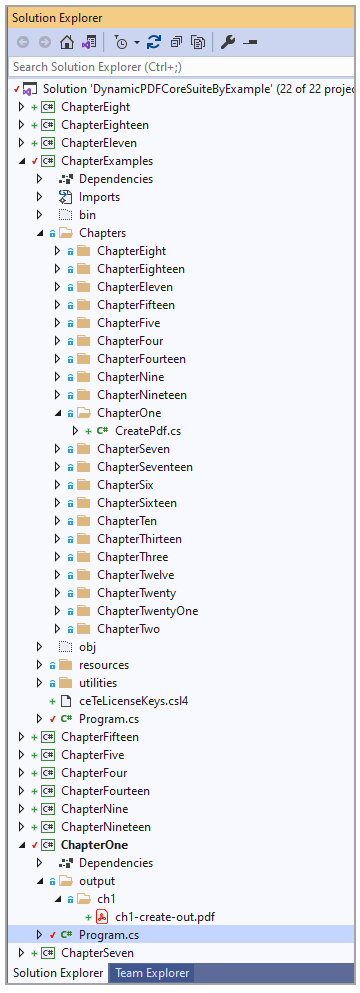
\includegraphics[scale=0.5]{figures/ch1/fig3}\caption{Solution structure.}\label{mar:DynamicPdfCoreSuiteByExample-sol}
\end{marginfigure}


\subsection{Example Solution}

You can find the sample code for the book's solution at GitHub: https://github.com/jamesabrannan/DynamicPDFCoreSuiteByExample. Each chapter's content consist of a separate project and a folder within the  \texttt{ChapterExamples} project. For example, the \texttt{ChapterOne} project contains the project for this chapter while the examples are in the \texttt{Chapters/ChapterOne} folder in the
\texttt{ChapterExamples} project. 

All resources are contained in the \texttt{ChapterExamples} project's
\texttt{resources} folder and are further organized with sub-folders
for each chapter. Each chapter's project has its own \texttt{output}
folder where it places the chapter's produced PDF documents.Each chapter has a corresponding standalone project. However, in
the \texttt{ChapterExamples} project, you can also run all the book's
examples simultaneously. This creation pattern is repeated for all
chapters in this book.
\begin{figure}
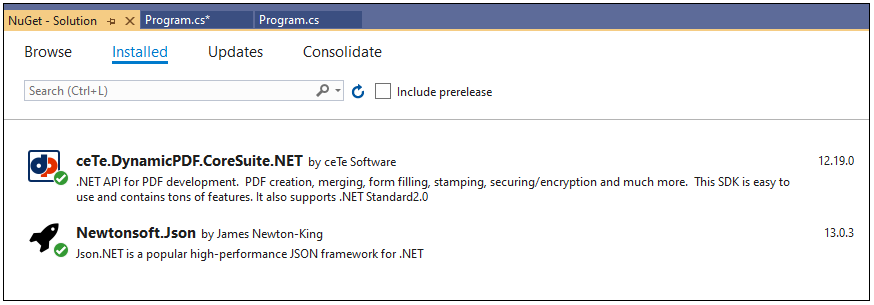
\includegraphics[scale=0.45]{figures/ch1/fig2}\caption{NuGet packages used by book's project.}\label{mar:Nuget-packages-used}
\end{figure}

The solution on GitHub includes the required NuGet packages, \texttt{cete.DynamicPDF.CoreSuite.NET}\index{cete.DynamicPDF.CoreSuite.NET}
and \texttt{Newtonsoft.Json} (Figure \ref{mar:Nuget-packages-used}). Be
certain to ensure you have the latest NuGet versions installed. At the
time of this writing, I used version 12.19.0 for DynamicPDF Core Suite
and 12.0.3 for Newtonsoft.Json. I also used .NET 5 and Visual Studio 2019, although using this combination is not required.

\section{The Portable Document Format (PDF) by Adobe}\index{The Portable Document Format (PDF) by Adobe}

Virtually everyone recognizes the universal symbol for documents created
using the Portable Document Format (PDF), or simply referred to as
PDF (Figure \ref{mar:The-Adobe-PDF}). The PDF format was first released
by Adobe Inc. in June 1993 as a way to present formatted documents
in a platform independent manner. 
\begin{marginfigure}
\centering
\includegraphics[scale=1]{figures/ch1/PDF_file_icon\lyxdot svg}\caption{The Adobe PDF icon.}\label{mar:The-Adobe-PDF}

\end{marginfigure}

\index{PDF}PDF is a file format used to present and exchange documents reliably,
independent of software, hardware, or operating system. PDF documents
can contain text, images, links, and interactive elements such as
forms, annotations, and multimedia. This format is widely used for
sharing documents across different platforms while maintaining their
original formatting and appearance. You can create PDF files from
various sources such as scanned documents, word processing software,
and design applications. Additionally, PDFs can be encrypted, digitally
signed, and secured with various permissions to control access and
usage. 

Since its release in 1993, the PDF specification has evolved significantly.
It was initially proprietary and controlled by Adobe, but it became
an ISO open standard in 2008 (ISO 32000-1:2008). There are two primary
ISO standards for PDF documents, ISO 32000-1:2008 and ISO 32000-2:2020.

A PDF document combines text, vector graphics, and bitmap graphics
to create an electronic document. A PDF file combines the assets stored
in the PDF document using built-in storage and a subset of Postscript
rendering instructions for combining and displaying its assets.

A PDF document can be linearized (optimized) or non-linearized. PDF documents can also conform to standards such as PDF/UA or PDF/A,
which are crucial for ensuring accessible documents or for facilitating
long-term storage. The PDF/Universal Accessibility (PDF/UA) ISO standard
provides standards for ensuring accessibility for people with disabilities
requiring screen readers, magnifiers, and other similar technologies.
The PDF/Archive (PDF/A) ISO standard provides standards for ensuring
PDF documents are suitable for long-term archiving.

Refer to Adobe's ample online documentation to learn more about the PDF standard. Alternatively, you can use Wikipedia as a starting point for further exploration. Now, let's get to coding "Hello World."

\section{Creating Your First PDF}

Let’s start by illustrating how to create a simple PDF document from
scratch. The steps in the following section provide a good roadmap when creating your PDF documents.\begin{marginfigure}
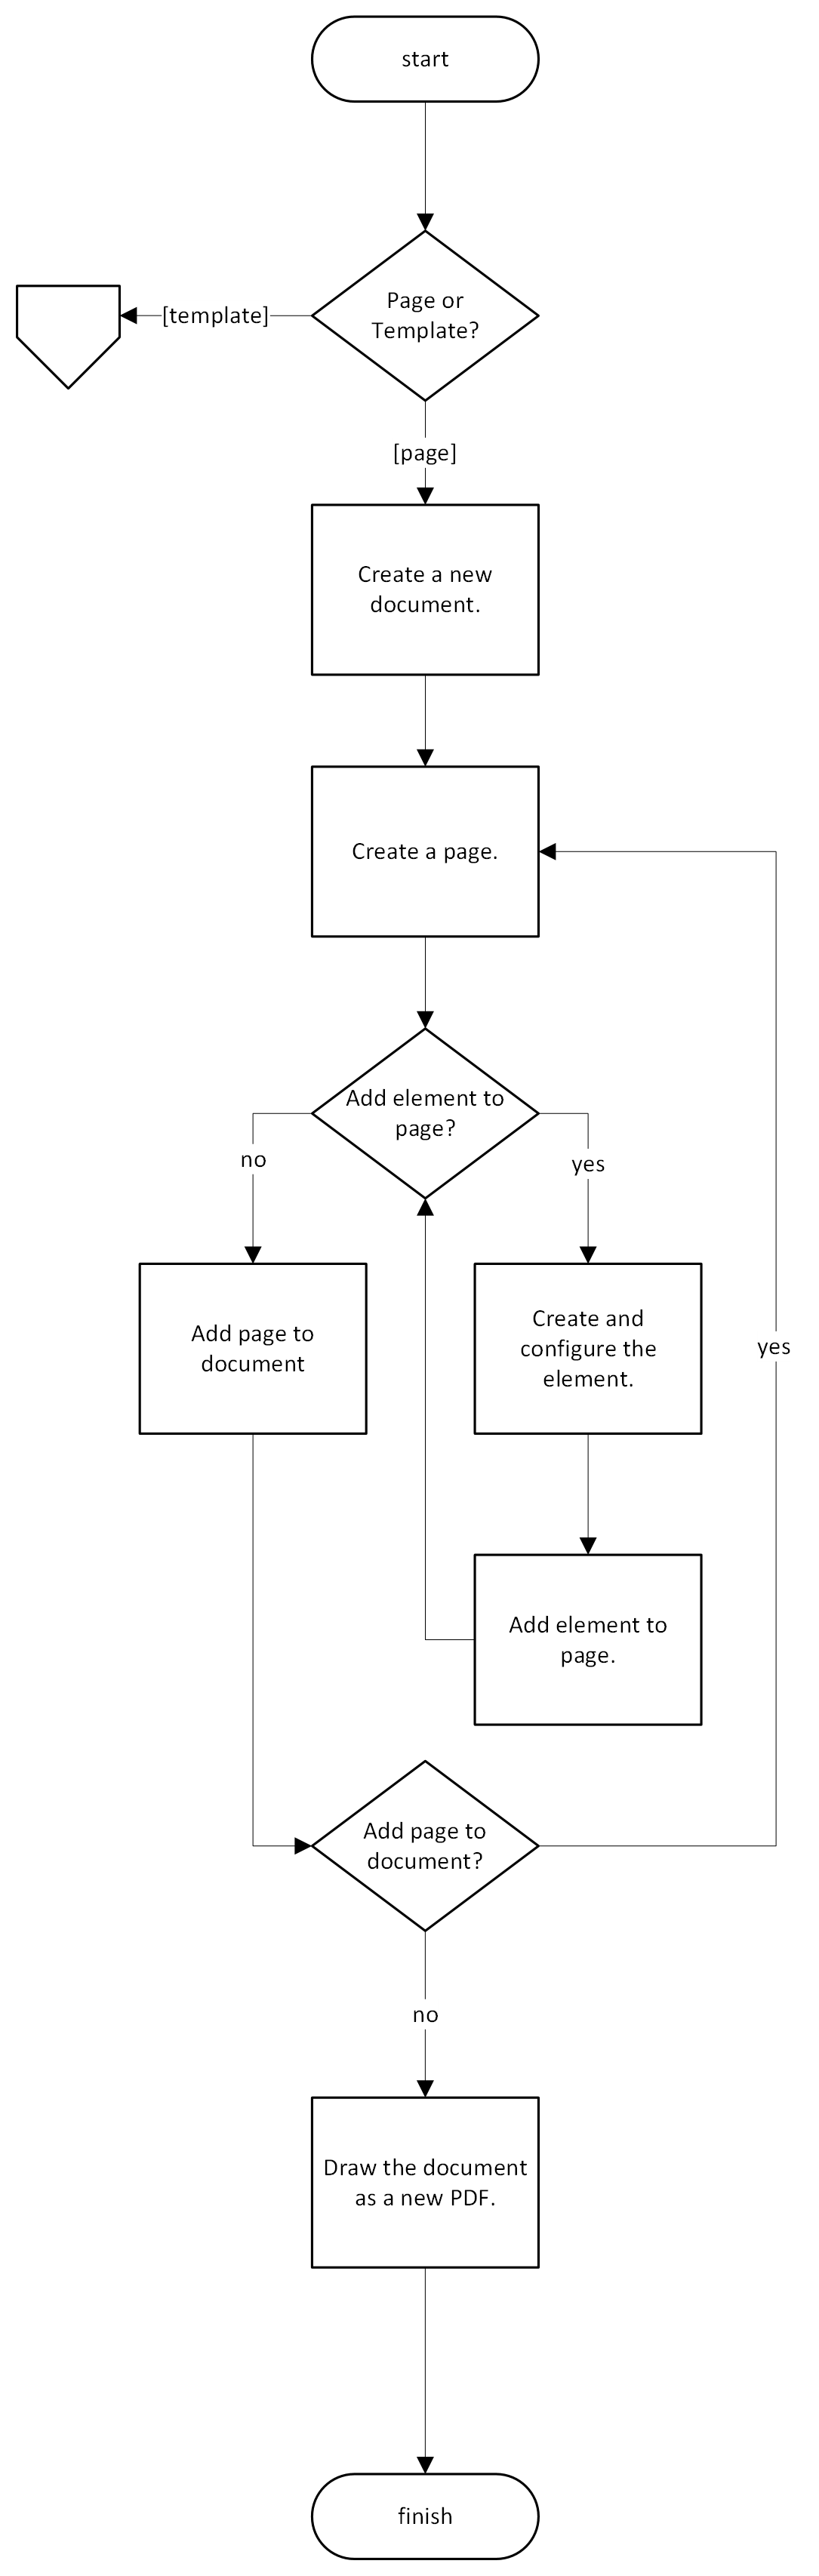
\includegraphics[scale=0.6]{figures/ch1/create-steps}\caption{Common processing steps in creating a PDF document.}\label{mar:Common-processing-steps-1}
\end{marginfigure}

\subsection{Creating a PDF}\label{subsec:steps-Creating-a-PDF}\index{Creating a PDF}
The \texttt{CreatePdf} class (Listing \ref{lis:Creating-a-PDF}) has
a static method named \texttt{Create} that takes the path to the created
PDF document. When creating a new PDF all PDF documents using Core Suite begins with
a new \texttt{Document} instance. The method then performs the following processing steps; these steps are common for creating any PDF document when using Core Suite (Figure \ref{mar:Common-processing-steps-1}).

\begin{enumerate}
\item Create a new \texttt{Document}\index{Document} object instance.
\item Create one or more \texttt{Page}\index{Page} instances.
\item Add elements from the \texttt{PageElements}\index{PageElements} namespace to the desired
\texttt{Page}\index{Page} instance.
\item Add the \texttt{Page}\index{Page} instances to the \texttt{Document}\index{Document} instance's
\texttt{Pages}\index{Pages} collection.
\item Call the \texttt{Document}\index{Document} instance's \texttt{Draw}\index{Draw} method to produce
the new PDF document (Figure \ref{fig:A-simple-PDF}).
\end{enumerate}
\bgroup\inputencoding{latin9}
\begin{lstlisting}[caption={Creating a PDF from scratch.},label={lis:Creating-a-PDF},basicstyle={\small},breaklines=true]
using ceTe.DynamicPDF;
using ceTe.DynamicPDF.PageElements;

namespace ChapterExamples.Chapters.ChapterOne
{
    public class CreatePdf
    {
        public static void Create(string outputPath)
        {
            Document myDocument = new();
            Page myPage = new();
            myDocument.Pages.Add(myPage);
            Label myLabel = new("Hello DynamicPDF Core Suite.", 50, 50, 200, 50);
            myPage.Elements.Add(myLabel);
            myDocument.Draw(outputPath);
        }       
    }
}
\end{lstlisting}
\leavevmode\egroup

\begin{figure}
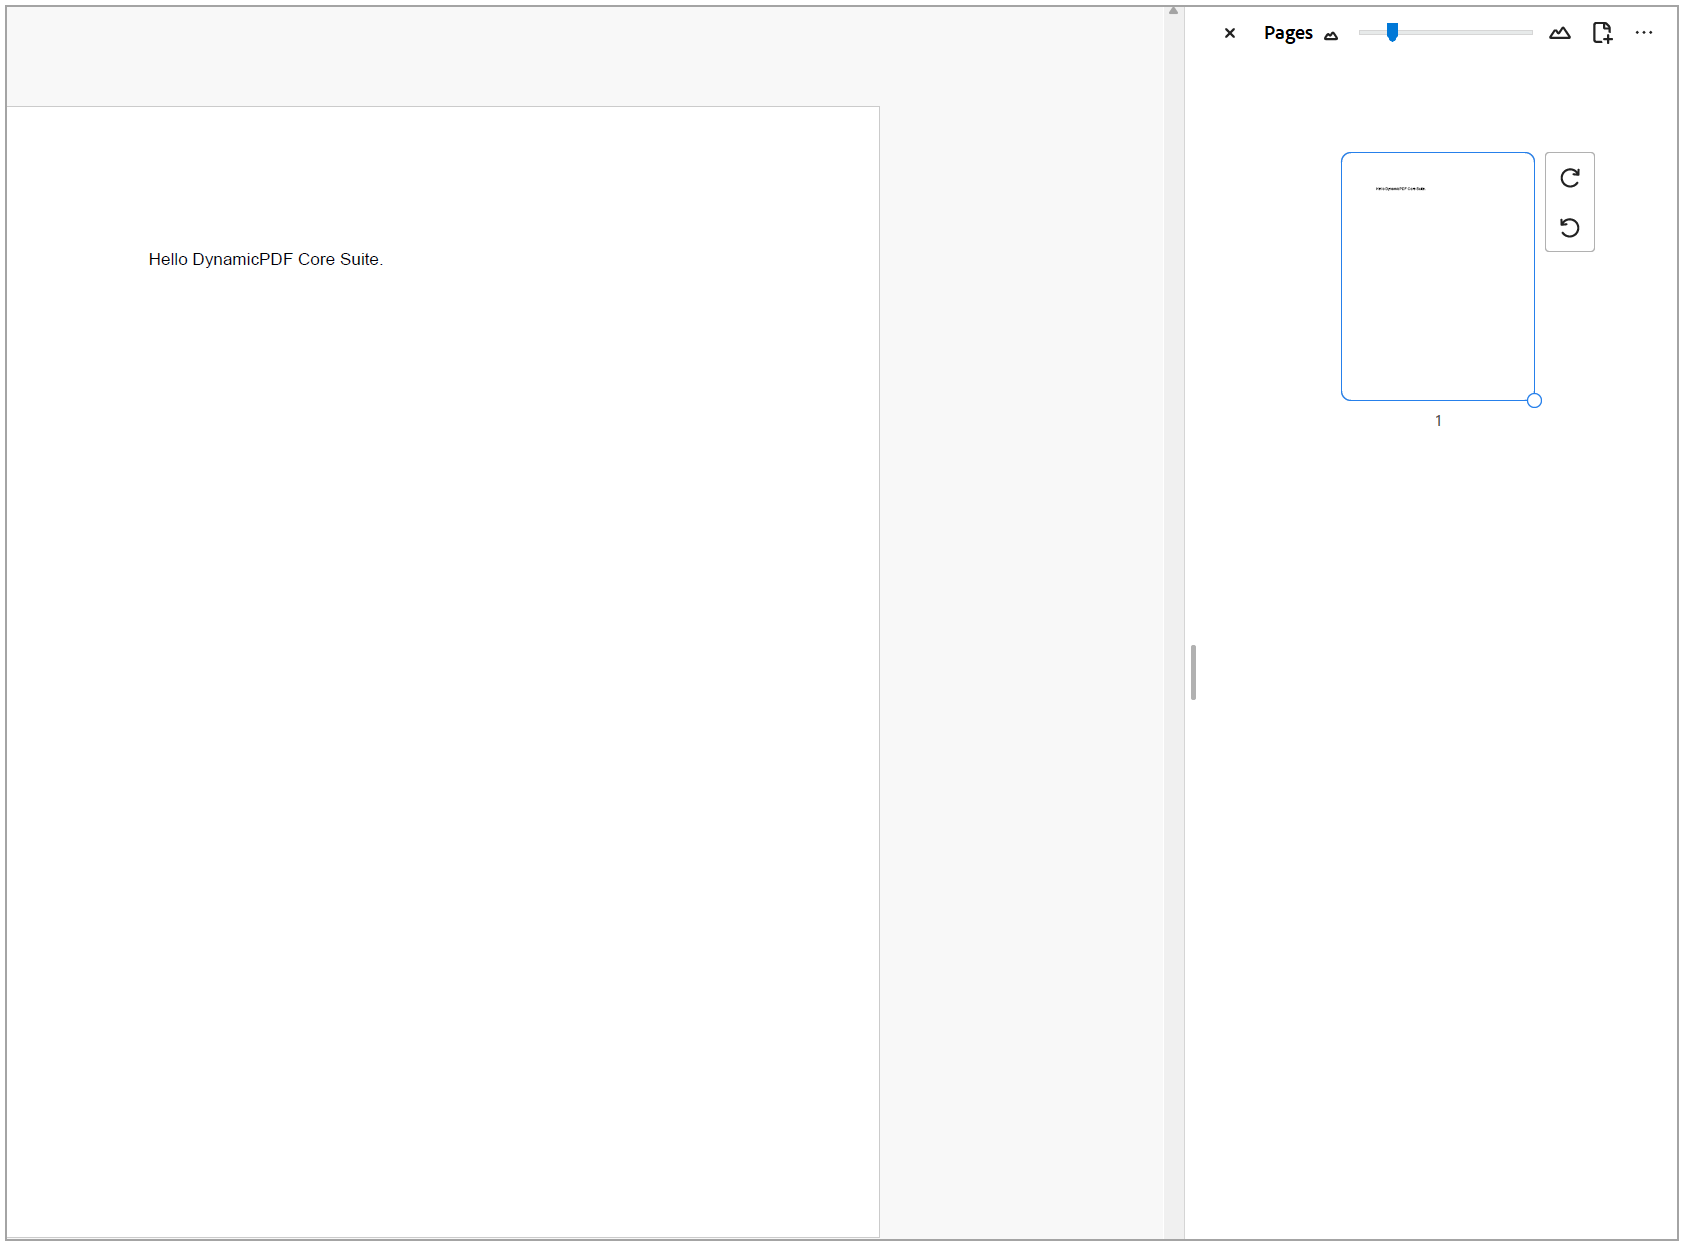
\includegraphics[scale=0.3]{figures/ch1/fig4}\caption{A simple PDF document created by Listing \ref{lis:Creating-a-PDF}.}\label{fig:A-simple-PDF}
\end{figure}

All elements, including charts, barcodes, forms, and tables, inherit
from the \texttt{ceTe.DynamicPDF.PageElement}\index{ceTe.DynamicPDF.PageElement} class.\index{ceTe.DynamicPDF.PageElement} In Listing \ref{lis:Creating-a-PDF}
you create an instance of \texttt{ceTe.DynamicPDF.PageElements.Label}\index{ceTe.DynamicPDF.PageElements.Label}
class and add it to our page. Classes inheriting from the\texttt{
PageElements} parent class include the following name-spaces:
\begin{itemize}
\item \texttt{ceTe.DynamicPDF.PageElements.BarCoding}\index{ceTe.DynamicPDF.PageElements.BarCoding},
\item \texttt{ceTe.DynamicPDF.PageElements.Charting}\index{ceTe.DynamicPDF.PageElements.Charting},
\item \texttt{ceTe.DynamicPDF.PageElements.Forms}\index{ceTe.DynamicPDF.PageElements.Forms}, and
\item \texttt{ceTe.DynamicPDF.PageElements.Html}\index{ceTe.DynamicPDF.PageElements.Html}.
\end{itemize}
You will see examples using all four of these namespaces in later
chapters. However, as Listing \ref{lis:Creating-a-PDF} illustrates,
when using Core Suite, creating a PDF always begins with a new \texttt{Document}\index{Document}
instance 
\section{Modifying Your First PDF}
Now that you have seen how to create your first PDF document, let's switch to modifying three pre-existing PDF documents by merging them together. Let's also add a new page to the merged document. \marginnote{Modifying a PDF almost always requires performing the steps in Figure  \ref{mar:mod-common-processing-steps-1}}
\begin{figure}
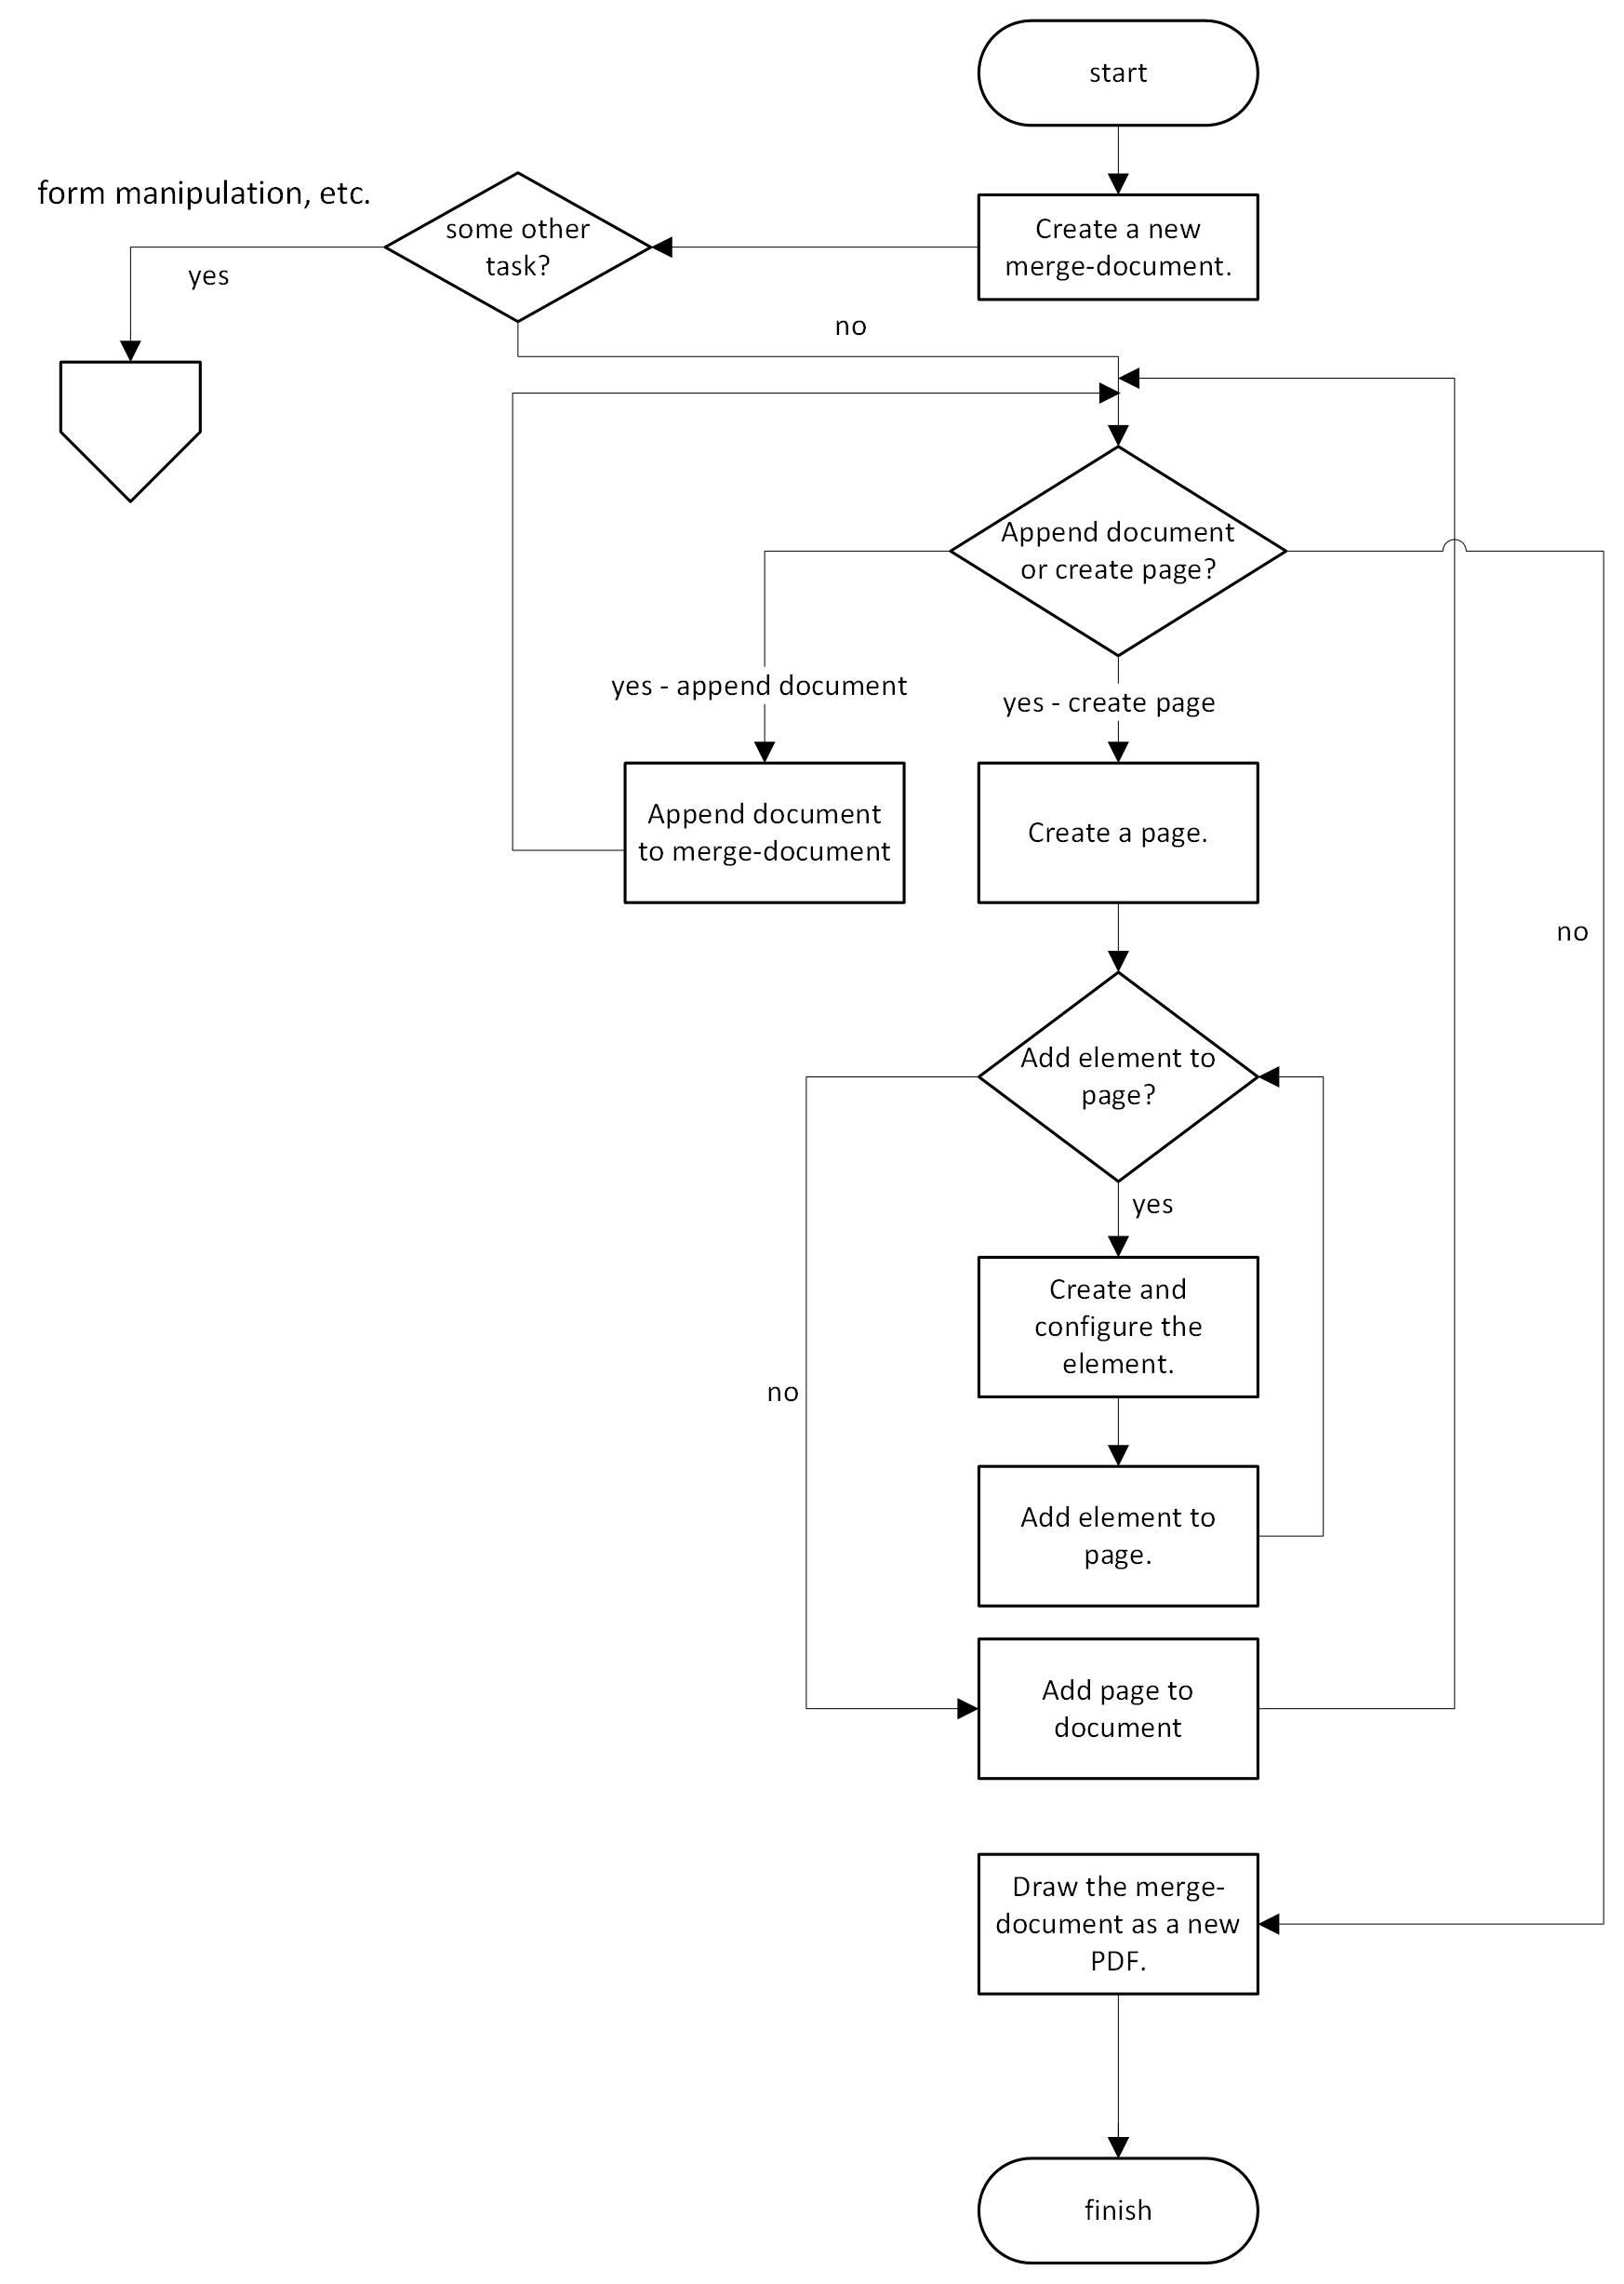
\includegraphics[scale=0.75]{figures/ch1/modify-diagram}\caption{Common processing steps when modifying a PDF document.}\label{mar:mod-common-processing-steps-1}
\end{figure}
\subsection{Modifying a PDF}\label{subsec:steps-modifying-a-PDF}
Modifying an existing PDF document can entail completing an existing PDF form, extracting content from a PDF, and other tasks.  However, let's limit ourself to merging and appending one or more PDF documents and adding a new page. 

Creating a new PDF document from existing PDF documents consists of the following steps.
\begin{enumerate}
\item Create a new \texttt{MergeDocument}\index{MergeDocument} instance.\index{MergeDocument}
\item Append zero or more \texttt{PdfDocument}\index{PdfDocument} instances.\index{PdfDocument}
\item Add zero or more new \texttt{Page}\index{Page} instances to the \texttt{MergeDocument}\index{MergeDocument} instance.
\item Call the \texttt{MergeDocument}\index{MergeDocument} instance's \texttt{Draw}\index{Draw} method to produce
the new PDF document of the appended documents.
\end{enumerate}
Although, as you will see in Part \ref{part:modifying-pdf-doc}, there are many more modifications you can make to existing PDF documents, you will almost always perform the steps in Figure  \ref{mar:mod-common-processing-steps-1}.
For example, in Listing \ref{lis:modifying-a-PDF} you merge three documents together by first creating a new \texttt{MergeDocument}\index{MergeDocument} instance from the two existing PDF documents and then append a third. After merging the three documents, you create a new  \texttt{Page}\index{Page} instance, add a label to the page, and then insert the page as the first page of the \texttt{MergeDocument}\index{MergeDocument} instance. You then write the \texttt{MergeDocument}\index{MergeDocument} instance as a new PDF document (Figure \ref{mar:merged-pdf}).
\begin{figure}
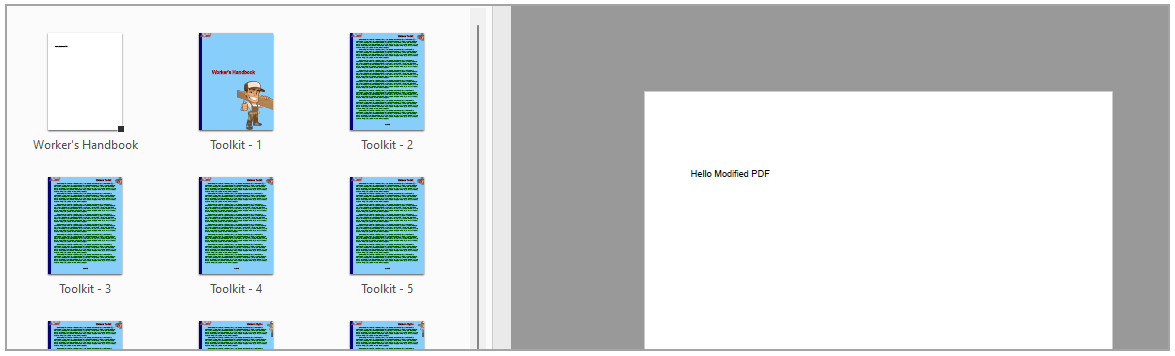
\includegraphics[scale=0.35]{figures/ch1/fig7}\caption{Merged PDF document.}\label{mar:merged-pdf}
\end{figure}
\bgroup\inputencoding{latin9}
\begin{lstlisting}[caption={Modifying a PDF.},label={lis:modifying-a-PDF},basicstyle={\small},breaklines=true]
using ceTe.DynamicPDF;
using ceTe.DynamicPDF.Merger;
using ceTe.DynamicPDF.PageElements;

namespace ChapterExamples.Chapters.ChapterOne
{
    public class SimpleMerge
    {

        public static void Modify(string resourcePath, string outputPath)
        {
            MergeDocument mergedDoc = MergeDocument.Merge(resourcePath + "doc1.pdf", resourcePath + "doc2.pdf");
            mergedDoc.Append(resourcePath + "doc3.pdf");
            Page page = new Page(PageSize.Letter);
            page.Elements.Add(new Label("Hello Modified PDF", 10, 50, 150, 0));
            mergedDoc.Pages.Insert(0, page);
            mergedDoc.Draw(outputPath + "simple-merge-out.pdf");
        }
    }
}
\end{lstlisting}
\leavevmode\egroup
Modifying existing PDF documents primarily rely on the following namespaces
\begin{itemize}
\item \texttt{ceTe.DynamicPDF.Merger}\index{ceTe.DynamicPDF.Merger} and \index{ceTe.DynamicPDF.Merger}
\item \texttt{ceTe.DynamicPDF.Merger.Forms}\index{ceTe.DynamicPDF.Merger.Forms}.\index{ceTe.DynamicPDF.Merger.Forms}
\end{itemize}
But, when merging, you can also use the other namespaces listed earlier when creating new pages and adding them to pre-existing PDF documents or when placing extracted elements from one PDF to a new merged document. For example, in Listing \ref{lis:modifying-a-PDF} you used the  \texttt{ceTe.DynamicPDF}\index{ceTe.DynamicPDF} and  \texttt{ceTe.DynamicPDF.PageElements}\index{ceTe.DynamicPDF.PageElements} namespaces to create a new page which you then added to the \texttt{MergeDocument}\index{MergeDocument} instance.

Modifying an existing PDF is arguably more involved then creating a new PDF. Not only do you have all the merging functionality of Core Suite, you also have all the creation functionality. As we see in Part \ref{part:modifying-pdf-doc}, you can combine existing PDF documents and new PDF documents. But for now, as Listing  \ref{lis:modifying-a-PDF} and Figure  \ref{mar:mod-common-processing-steps-1} illustrates, modifying an existing PDF almost always consists of merging two or more PDF documents into a new combined PDF document and adding zero or more new pages containing new content.

\section{Summary}

In this chapter, you were introduced to the DynamicPDF Core Suite for
.NET and what it can accomplish. You created your first PDF document
from scratch. And you merged three PDF documents to create a new PDF Document. We also learned the primary namespaces used by Core Suite and you saw how most tasks you will accomplish using Core Suite are essentially the steps listed in Figure \ref{fig:A-simple-PDF} and Figure \ref{mar:mod-common-processing-steps-1}. 

Of course, you can do much with Core Suite, as you will learn throughout
the remainder of this book. But throughout Part \ref{part:Create-PDF-Documents}, recall the diagram
in Figure \ref{mar:Common-processing-steps-1} and remember these
common processing steps as you work through the book and its examples. Then, when we get to Part \ref{part:modifying-pdf-doc}, we can examine modifying PDF documents, as the steps are more involved. But fundamentally the steps are similar to those in Figure \ref{mar:mod-common-processing-steps-1}. We will discuss modifing PDF documents more later, for now, let's get started with creating new PDF documents.

\DPpart{Creating PDF Documents}{part:Create-PDF-Documents}
\color{white}
\chapter{Documents}\label{chap:Creating-PDF-Documents}
\color{black}
\BgThispage
\vspace{8.0em}
\lettrine[lines=2,lhang=0.1]{I}{n} this chapter, you learn about creating documents using the \texttt{Document} class. We build upon what you learned in Chapter \ref{chap:Introducing-DynamicPDF-Core}
by laying out pages of a document using coordinates, allowing you precise control
of your PDF document's appearance. You also learn about setting a PDF
document's properties and how to alter the initial appearance of your
document in a PDF reader such as Adobe Acrobat Reader.\marginnote{Understanding page dimensions and how to place elements on a page is critical for creating professional appearing PDF documents. }

We then devote the remainder of the chapter to page dimensions and page layout. Although we
spend considerable time on page dimensions, coordinates, and precise
page layout, understanding page dimensions and how to place elements
on a page is critical if you wish to create professionally appearing
PDF documents. 

By the end of this chapter you will have good understanding of creating and properly laying out a PDF document. So let's get started!

\section{Creating a Document}
The \texttt{Document}\index{Document} class is central to everything you do when using
Core Suite to create new PDF documents. In the last chapter we outlined
common steps used when creating PDF documents from scratch (Figure
\ref{mar:Common-processing-steps-1}). The steps are so important,
and so common, they bear repeating here.
\begin{enumerate}
\item Create a new \texttt{Document}\index{Document} object instance.
\item Create one or more \texttt{Page}\index{Page} instances.
\item Add elements from the \texttt{PageElements}\index{PageElements} namespace to the desired
\texttt{Page}\index{Page} instance.
\item Add the page objects to the document object's \texttt{Pages}\index{Pages} collection.
\item Call the document object's \texttt{Draw}\index{Draw} method to produce the new
PDF document (Figure \ref{fig:A-simple-PDF}).
\end{enumerate}
The \texttt{Document}\index{Document} class represents a PDF document. You always
begin by creating a \texttt{Document}\index{Document} instance when creating a new
PDF; it is the basic building block for all PDF documents. The Document
class has numerous methods and properties which you will learn about
throughout this book. Through this class you set everything from a
document's metadata to its collections containing pages, outlines,
and other elements. 

After creating a new \texttt{Document}\index{Document} instance, you then add one
or more \texttt{Page}\index{Page} class instances to build a complete document.
By adding pages to a document, you create a PDF document. But you
always begin with a \texttt{Document}\index{Document} instance.

\subsection{Document Class}

The \texttt{Document}\index{Document} class has one constructor that takes no parameters.
We don't provide a code example using the \texttt{Document}\index{Document} class,
lest you attempt to do this yourself and generate an error (Figure
\ref{mar:Attempting-to-output}). 
\begin{marginfigure}

\includegraphics[scale=0.33]{figures/ch2/error}\caption{Attempting to output a document with no pages.}\label{mar:Attempting-to-output}

\end{marginfigure}
 You must add at least one \texttt{Page}\index{Page} instance to a document before
you can create a PDF document.

\subsection{The Draw Method}

After building a document, you call one of the \texttt{Document}\index{Document} instance's
provided \texttt{Draw}\index{Draw} methods. The \texttt{Document}\index{Document} class has three
overloads for the \texttt{Draw}\index{Draw} method, allowing you to write a PDF
document to a file, to a stream, or a byte-array.\marginnote{In this book we limit our examples to using the \texttt{Draw} method to output to a file.}
\begin{itemize}
\item \texttt{Draw()} - Writes document to a byte array.
\item \texttt{Draw(Stream)} - Writes document to a Stream.
\item \texttt{Draw(String)} - Writes document to a file using provided path.
\end{itemize}
Drawing a PDF document to a stream or array allows incorporating the
PDF into a larger application such as a web page.

\section{Adding Pages}

After creating a \texttt{Document}\index{Document} instance, you add one or more pages
to it through its \texttt{Pages}\index{Pages} property. This property is a \texttt{PageList}\index{PageList}
of \texttt{Page}\index{Page} instances. You add pages through the \texttt{Document}\index{Document}
instance's \texttt{Pages}\index{Pages} property's \texttt{Pages.Add(Page)} method.
For example, in Listing \ref{lis:ch2Creating-a-simple} you create
two blank pages and add them to the document. Of course, it doesn't create a
very interesting PDF document, as it consists of two blank pages.

\bgroup\inputencoding{latin9}
\begin{lstlisting}[caption={Creating a simple PDF Document.},label={lis:ch2Creating-a-simple},basicstyle={\small\ttfamily},breaklines=true]
using ceTe.DynamicPDF;

namespace ChapterExamples.Chapters.ChapterTwo
{
    class DocumentPage
    {
        public static void Create(string resourcePath, string outputPath)
        {
            Document myDoc = new();
            Page myPg = new();
            Page myPg2 = new();
            myDoc.Pages.Add(myPg);
            myDoc.Pages.Add(myPg2);
            myDoc.Draw(outputPath);
        }
    }
}
\end{lstlisting}
\leavevmode\egroup


\subsection{Page Class}
\marginnote{All measurements in Core Suite use points.}
You add pages to a document by creating and adding \texttt{Page}\index{Page} instances.
A \texttt{Page}\index{Page} represents a page in a PDF document. A \texttt{Page}\index{Page}
has properties abstracting its dimensions, size, and orientation with
the \texttt{PageDimensions}\index{PageDimensions}, \texttt{PageSize}\index{PageSize}, and \texttt{PageOrientation}\index{PageOrientation}
classes. \marginnote{A page's defaults values are: 50 pt margins, 1008 pt width, and 612 pt
height.}The \texttt{Page}\index{Page} class has eight different overloads for its constructor:
\texttt{Page()}, \texttt{Page(PageDimensions)}, \texttt{Page(PageSize)},
\texttt{Page(PageSize, PageOrientation)}, \texttt{Page(PageSize, PageOrientation,
Single)}, \texttt{Page(PageSize, Single)}, \texttt{Page(Single, Single)},
and \texttt{Page(Single, Single, Single)}. These constructor parameters
initialize a page's size, orientation, and layout.

\subsection{Page Orientation, Size, and Margins}

The \texttt{PageDimensions}\index{PageDimensions} class represents a page's dimensions.
A page's dimensions are measured in points. You set a page's height,
width, and margins using the \texttt{PageDimensions}\index{PageDimensions} class. You can
also set the page's properties directly or through the \texttt{PageDimensions}\index{PageDimensions}
class's constructor. For example, Listing \ref{lis:ch2-multipage-Creating-a-PDF-1}
creates a five-page document of varying dimensions.
\begin{marginfigure}

\includegraphics[scale=0.3]{figures/ch2/fig2}\caption{Listing \ref{lis:ch2-multipage-Creating-a-PDF-1} produces a five-page
document.}\label{mar:ch2-Listing-produces-a}
\end{marginfigure}
 The first page sets its dimensions directly using a \texttt{PageDimensions}\index{PageDimensions}
instance that sets its size as legal and orientation as landscape.
The second page reuses the first page's dimensions, but instead of
setting the dimension to the page, it passes the dimensions in its
constructor. The third page sets its size, orientation, and margins
directly. The fourth page only sets its width and height, leaving
the other dimensions at their default values. Finally, the fifth page
sets its page size as an envelope. The \texttt{Document} instance then writes the created
PDF document to a file (Figure \ref{mar:ch2-Listing-produces-a}).

\bgroup\inputencoding{latin9}
\begin{lstlisting}[caption={Creating a PDF with different page sizes.},label={lis:ch2-multipage-Creating-a-PDF-1},basicstyle={\small\ttfamily},breaklines=true]
using ceTe.DynamicPDF;

namespace ChapterExamples.Chapters.ChapterTwo
{
    class PageLayoutExample
    {
        public static void Create(string outputPath)
        {
            Document myDoc = new();
            PageDimensions myPgDm = new(PageSize.Legal, PageOrientation.Landscape);
            myPgDm.BottomMargin = 50;
            myPgDm.TopMargin = 50;
            myPgDm.LeftMargin = 100;
            myPgDm.RightMargin = 100;
            Page myPg = new();
            myDoc.Pages.Add(myPg);
            myPg.Dimensions = myPgDm;

            Console.WriteLine("Width: {0} Height: {1} LeftMargin: {2} RightMargin: {3} TopMargin: {4} BottomMargin: {5}", myPg.Dimensions.Width, myPg.Dimensions.Height, myPg.Dimensions.LeftMargin, myPg.Dimensions.RightMargin, myPg.Dimensions.TopMargin, myPg.Dimensions.BottomMargin);

            Page myPg2 = new(myPgDm);
            myDoc.Pages.Add(myPg2);
            Page myPg3 = new(PageSize.Postcard, PageOrientation.Landscape, 5F);
            myDoc.Pages.Add(myPg3);
            Page myPg4 = new(55, 90);
            myDoc.Pages.Add(myPg4);
            Page myPg5 = new(PageSize.Envelope10, PageOrientation.Landscape);
            myDoc.Pages.Add(myPg5);
            
            myDoc.Draw(outputPath);
        }
    }
}
\end{lstlisting}
\leavevmode\egroup

The \texttt{PageSize}\index{PageSize} class has constants for most page sizes, for
example Listing \ref{lis:ch2-multipage-Creating-a-PDF-1} used \texttt{Legal},
\texttt{Postcard} and \texttt{Envelope10}. It also used the \texttt{PageOrientation}
class, creating a page that was portrait and a page that was landscape.
Of course, you can set the page size directly by setting a page's
width and height using point values if you preferred.

You are not required to create a \texttt{PageDimensions}\index{PageDimensions} instance
explicitly. However, every page has a dimensions object populated
with default or assigned values. You access these values directly
through the page's \texttt{Dimensions}\index{Dimensions} property if you wish to view
or modify a page's size, orientation, or margins. For example, Listing
\ref{lis:ch2-multipage-Creating-a-PDF-1} prints the page's dimensions to the console as: 
{\ttfamily\bgroup\inputencoding{latin9}
\begin{lstlisting}[basicstyle={\small\ttfamily},breaklines=true]
Width: 1008 Height: 612 LeftMargin: 100
RightMargin: 100 TopMargin: 50 BottomMargin: 50
\end{lstlisting}
\leavevmode\egroup
}

\section{Coordinate System}\label{sec:Coordinate-System}

Every page has a coordinate system that specifies its width, height, and X and Y locations. These coordinates are measured in points. 
\begin{figure}
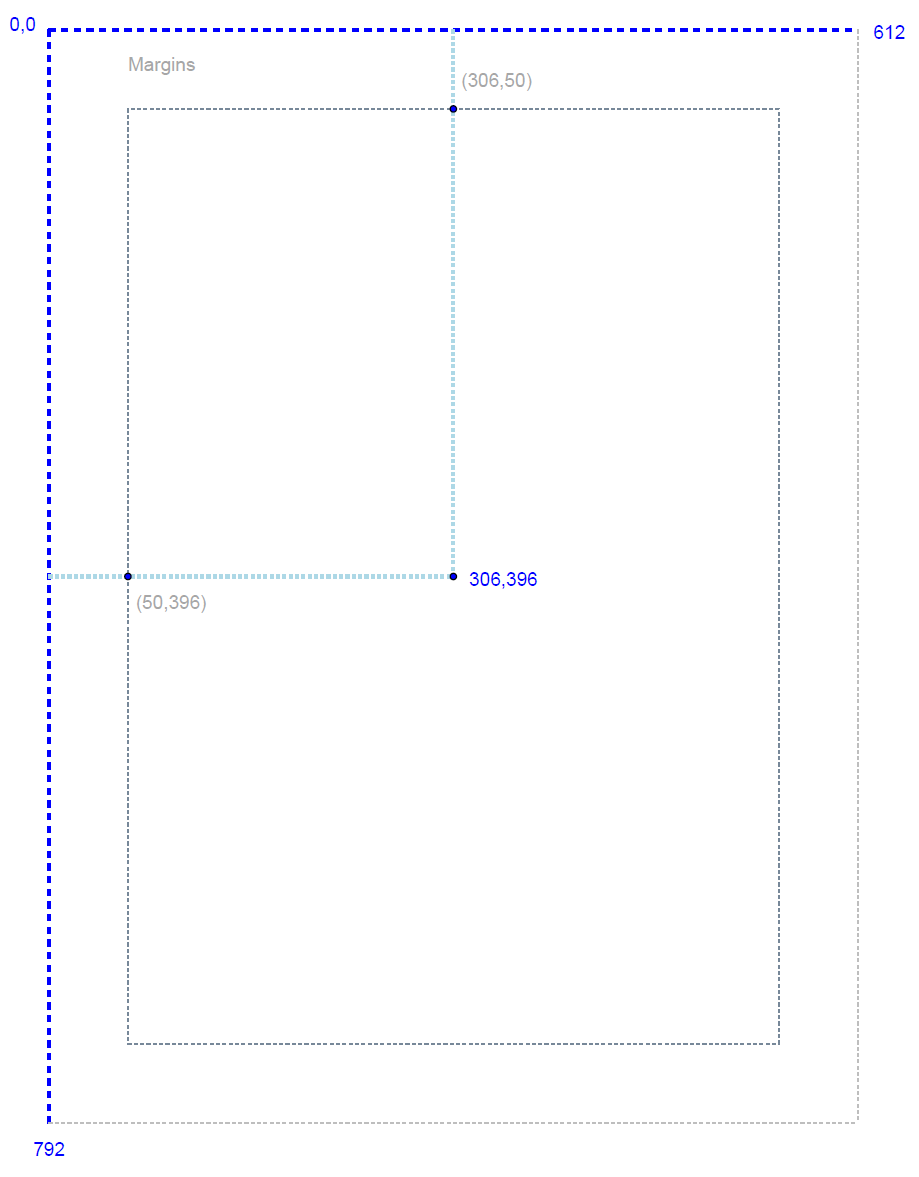
\includegraphics[scale=0.45]{figures/ch2/coords}\caption{Coordinates of an $8.5x11$ page with 50 point margins.}\label{fig:ch2-Coordinates-of-an}
\end{figure}
The coordinate system on a PDF page is called user space. This space
is a flat two-dimensional plane. You use this plane to determine the
layout of elements on a page when building a PDF, as Figure \ref{fig:ch2-Coordinates-of-an}
illustrates. The paper dimensions of an letter-sized page (8.5 x 11)
is 612 points by 792 points. The standard margin size is 50 points.
Thus, the center of the page is 306 points by 396 points. 

Table \ref{tab:Some-common-paper} lists several standard paper sizes
in points.

\begin{table}
\begin{tabular}{lccr}
\toprule 
Paper & Inches & Points & Centimeters\tabularnewline
\midrule
Letter & $8.5x11$ & $612x792$ & $21.59x27.94$\tabularnewline
Legal & $8.5x14$ & $612x1008$ & $21.59x35.56$\tabularnewline
Executive & $7.25x10.55$ & $522x756$ & $18.41x26.67$\tabularnewline
Envelope 10 & $4.13x9.5$ & $297x684$ & $10.48x24.13$\tabularnewline
\multicolumn{4}{r}{$point=inch*72,\;point=cm*28.35$}\tabularnewline
\bottomrule
\end{tabular}\caption{Some common paper sizes.}\label{tab:Some-common-paper}

\end{table}


\subsection{Coordinates Compared to Size}

One thing that might confuse you when starting to manually layout
pages and page elements is the difference between size and coordinates.
A page's or page element's height and width are measurements, not
locations. Its x and y values are locations. Measurement values
are relative to the page's dimensions while x and y locations are
relative to the page's margins. Although this distinction might seem obvious,
you must understand the implications this difference has for page
layout. For example, consider the code fragment in Listing \ref{lis:Adding-two-circles}.

\bgroup\inputencoding{latin9}
\begin{lstlisting}[caption={Adding three circles to a page.},label={lis:Adding-two-circles},basicstyle={\small\ttfamily},breaklines=true]
ceTe.DynamicPDF.PageElements.Circle c2 = new(0, 0, 8);
c2.FillColor = RgbColor.Blue;
myPg.Elements.Add(c2);

ceTe.DynamicPDF.PageElements.Circle c3 = new(myPg.Dimensions.Width - myPg.Dimensions.RightMargin, 0, 8);
c3.FillColor = RgbColor.Red;
myPg.Elements.Add(c3);

ceTe.DynamicPDF.PageElements.Circle c4 = new((myPg.Dimensions.Width - myPg.Dimensions.RightMargin - myPg.Dimensions.LeftMargin)/2, (myPg.Dimensions.Height - myPg.Dimensions.BottomMargin - myPg.Dimensions.TopMargin)/2, 8);
c4.FillColor = RgbColor.Green;
myPg.Elements.Add(c4);
\end{lstlisting}
\leavevmode\egroup

The three dots in Figure \ref{mar:ch2The-X-and} illustrate the resulting
PDF document's layout from Listing \ref{lis:Adding-two-circles}.
The blue dot's \texttt{x} and \texttt{y} values are $(0,0)$ and are hard coded, while
the red dot's \texttt{x} value is $612-50=562$ and \texttt{y} value is 0. The blue
dot's \texttt{x} and \texttt{y} position are relative to the margin, not the page. The
red dot, unlike the blue dot, uses relative measurements to position
itself on the page. It uses the width of the page and subtracts the
right margin from the width. But we forgot to account for the left
margin, and so the dot appears at the page's right edge. The green
dot's \texttt{x} value is $(612-50-50)/2=256$ and its \texttt{y} value is $(792-50-50)/2=346$,
or the center of the paper in relation the margin. It accomplishes
this precise location using relative measurements
\begin{figure}
\raggedright
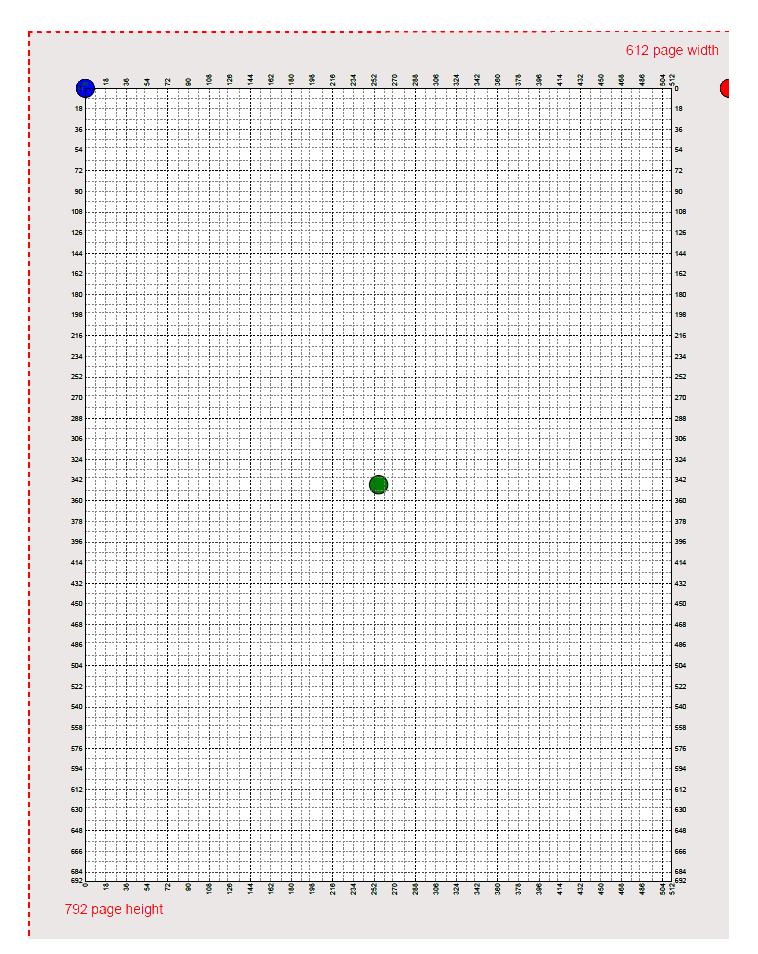
\includegraphics[scale=0.37]{figures/ch2/coordsize}\caption{The x and y coordinates compared to width and height.}\label{mar:ch2The-X-and}
\end{figure}

When laying out a page, always consider its margins. Use the right
and left margins when determining an element's \texttt{x} value. Also consider the
top and bottom margins when determining an element's \texttt{y} value. 

\subsection{Ignoring Margins and Relative Positioning}

All page elements have a \texttt{RelativeTo}\index{RelativeTo} and \texttt{IgnoreMargins}\index{IgnoreMargins}
property as of Core Suite's version 12. The \texttt{RelativeTo}\index{RelativeTo} property
by default is an element's top left and \texttt{IgnoreMargins}\index{IgnoreMargins} default value is
false. The following listing illustrates using both these properties
(Listing \ref{lis:Ignoring-an-image's}). The first image places itself
at $(0,0)$, only it ignores the document's margins. Because the image specifies that it ignores margins, it places the image under the layout grid and other image. The second image
does not ignore margins and so places itself relative to the document's margins (the default behavior).
Finally, the third image places itself just above the document's bottom
left. Figure \ref{fig:Ignoring-an-element's} illustrates the resultant
PDF document. 
\begin{figure}
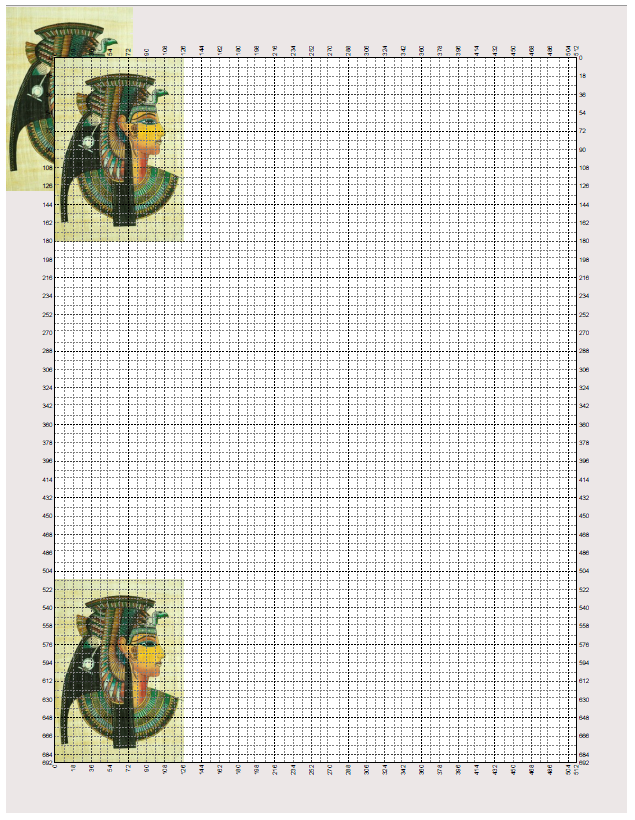
\includegraphics[scale=0.6]{figures/ch2/ignore-marg}\caption{Ignoring an element's margins and relative positioning example.}\label{fig:Ignoring-an-element's}

\end{figure}

\bgroup\inputencoding{latin9}
\begin{lstlisting}[caption={Ignoring an image's margins and relative positioning.},label={lis:Ignoring-an-image's},basicstyle={\small\ttfamily},breaklines=true]
using ceTe.DynamicPDF;
using ceTe.DynamicPDF.PageElements;

namespace ChapterExamples.Chapters.ChapterTwo
{
    public class IgnoreMarginsRelativeToExample
    {
        public static void Create(string resourcePath, string outputPath)
        {
            Document myDoc = new();
            Page myPg = new();
            myDoc.Pages.Add(myPg);

            Image image = new Image(resourcePath + "/egypt.jpg", 0, 0);
            image.ScaleX = 0.15F;
            image.ScaleY = 0.15F;
            image.IgnoreMargins = true;
            myPg.Elements.Add(image);

            Image image2 = new Image(resourcePath + "/egypt.jpg", 0, 0);
            image2.ScaleX = 0.15F;
            image2.ScaleY = 0.15F;
            myPg.Elements.Add(image2);

            Image image3 = new Image(resourcePath + "/egypt.jpg", 0, 0);
            image3.ScaleX = 0.15F;
            image3.ScaleY = 0.15F;
            image3.RelativeTo = RelativeTo.BottomLeft;
            image3.Y = -image3.Height;
            myPg.Elements.Add(image3);

            LayoutGrid layGrd = new();
            layGrd.Type = LayoutGrid.GridType.Standard;
            layGrd.ShowTitle = false;
            myPg.Elements.Add(layGrd);

            myDoc.Draw(outputPath);
        }
    }
}
\end{lstlisting}
\leavevmode\egroup
\begin{marginfigure}
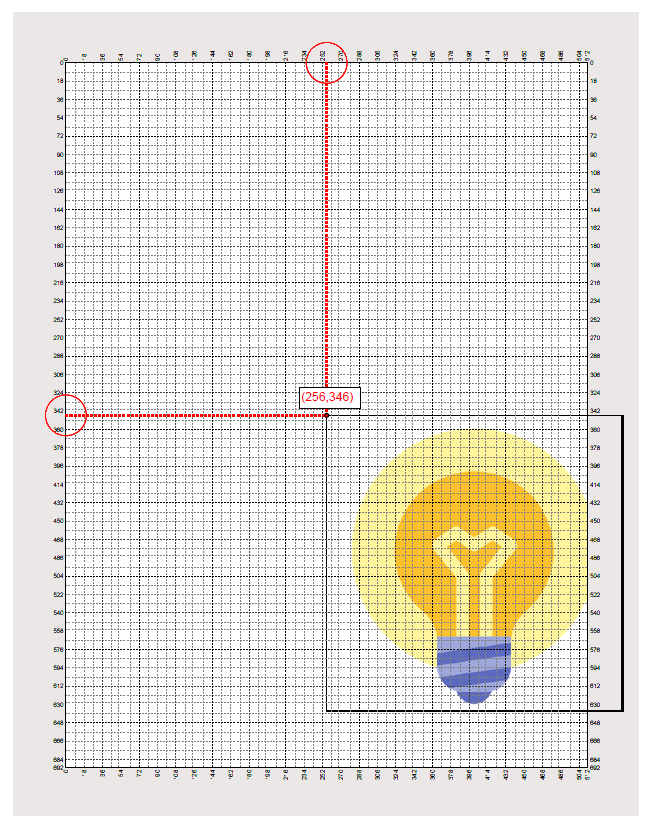
\includegraphics[scale=0.27]{figures/ch2/stepone-center}\caption{Step one of centering the image in Listing \ref{lis:Centering-an-image}.}\label{mar:Step-one-of}
\end{marginfigure}
\subsection{Example - Centering an Image}

Let's consider another example illustrating using measurements to lay out a
page (Listing \ref{lis:Centering-an-image}). 

Centering an image on a page is straightforward. Simply find the center
of the page and then set the image to vertical and horizontal alignment
at that point. Remember, an image's \texttt{x} and \texttt{y} coordinates are the top
left corner of the image. \begin{marginfigure}
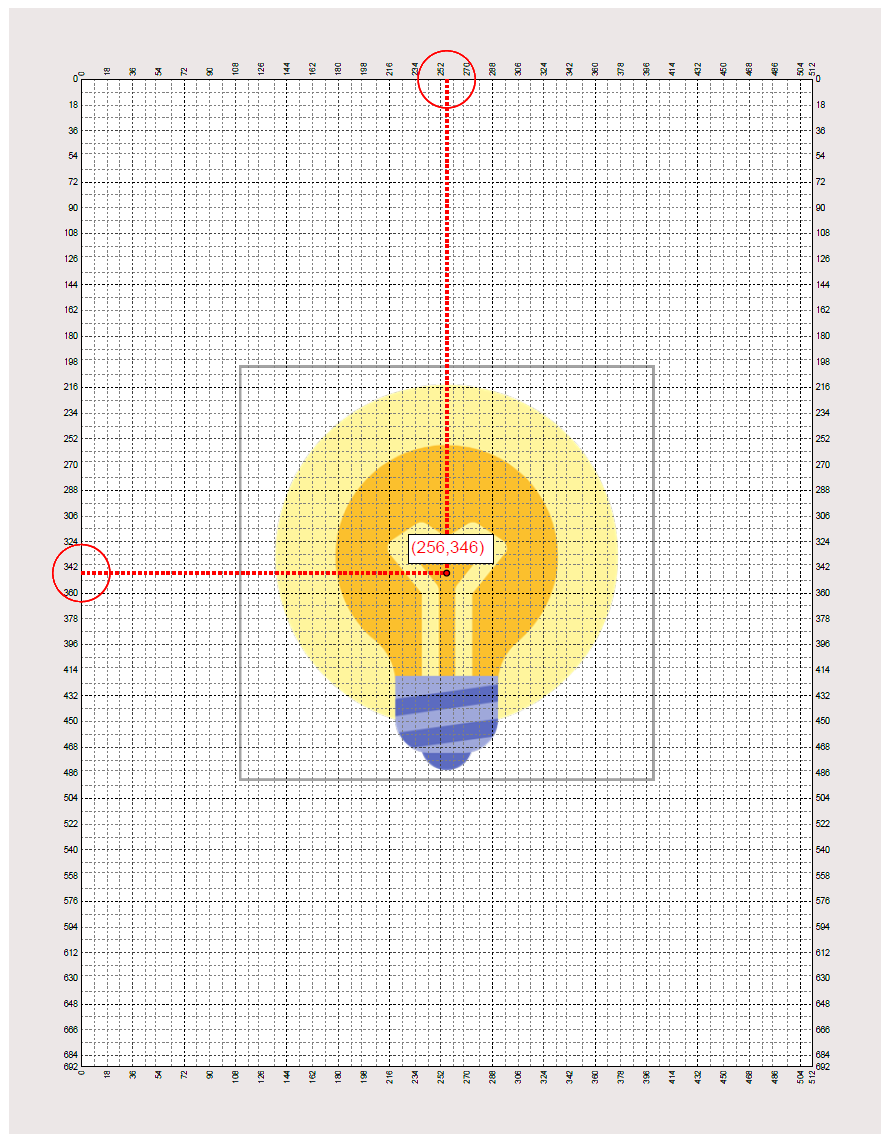
\includegraphics[scale=0.21]{figures/ch2/layoutgrid1}\caption{The image from Listing \ref{lis:Centering-an-image} centered on a
PDF document page.}\label{mar:center-The-image-from}
\end{marginfigure} For example, the image used in Listing \ref{lis:Centering-an-image}
first places the image with its top left corner at the center of the
page (Figure \ref{mar:Step-one-of}). It then centers the image by
setting the \texttt{Align}\index{Align} and \texttt{VAlign}\index{VAlign} property values to
\texttt{Center}\index{Center} (Figure \ref{mar:center-The-image-from}). 

\bgroup\inputencoding{latin9}
\begin{lstlisting}[caption={Centering an image on a page.},label={lis:Centering-an-image},basicstyle={\small\ttfamily},breaklines=true]
using ceTe.DynamicPDF;
using ceTe.DynamicPDF.PageElements;

namespace ChapterExamples.Chapters.ChapterTwo
{
    public class CoordinatesExample
    {
        public static void Create(string resourcePath, string outputPath)
        {
            Document myDoc = new();
            Page myPg = new();
            myDoc.Pages.Add(myPg);
            float centerX = (myPg.Dimensions.Width - myPg.Dimensions.LeftMargin - myPg.Dimensions.RightMargin) / 2;
            float centerY = (myPg.Dimensions.Height - myPg.Dimensions.TopMargin - myPg.Dimensions.BottomMargin) / 2;
            Image image = new Image(resourcePath + "/idea.png", centerX, centerY);
            image.VAlign = VAlign.Center;
            image.Align = Align.Center;
            myPg.Elements.Add(image);
            myDoc.Draw(outputPath);
        }
    }
}
\end{lstlisting}
\leavevmode\egroup
The resulting image from Listing \ref{lis:Centering-an-image} is shown in Figure \ref{mar:centering-image}.
\begin{figure}

\includegraphics[scale=0.30]{figures/ch2/fig11}\caption{Centering an image.}\label{mar:centering-image}
\end{figure}
\begin{marginfigure}
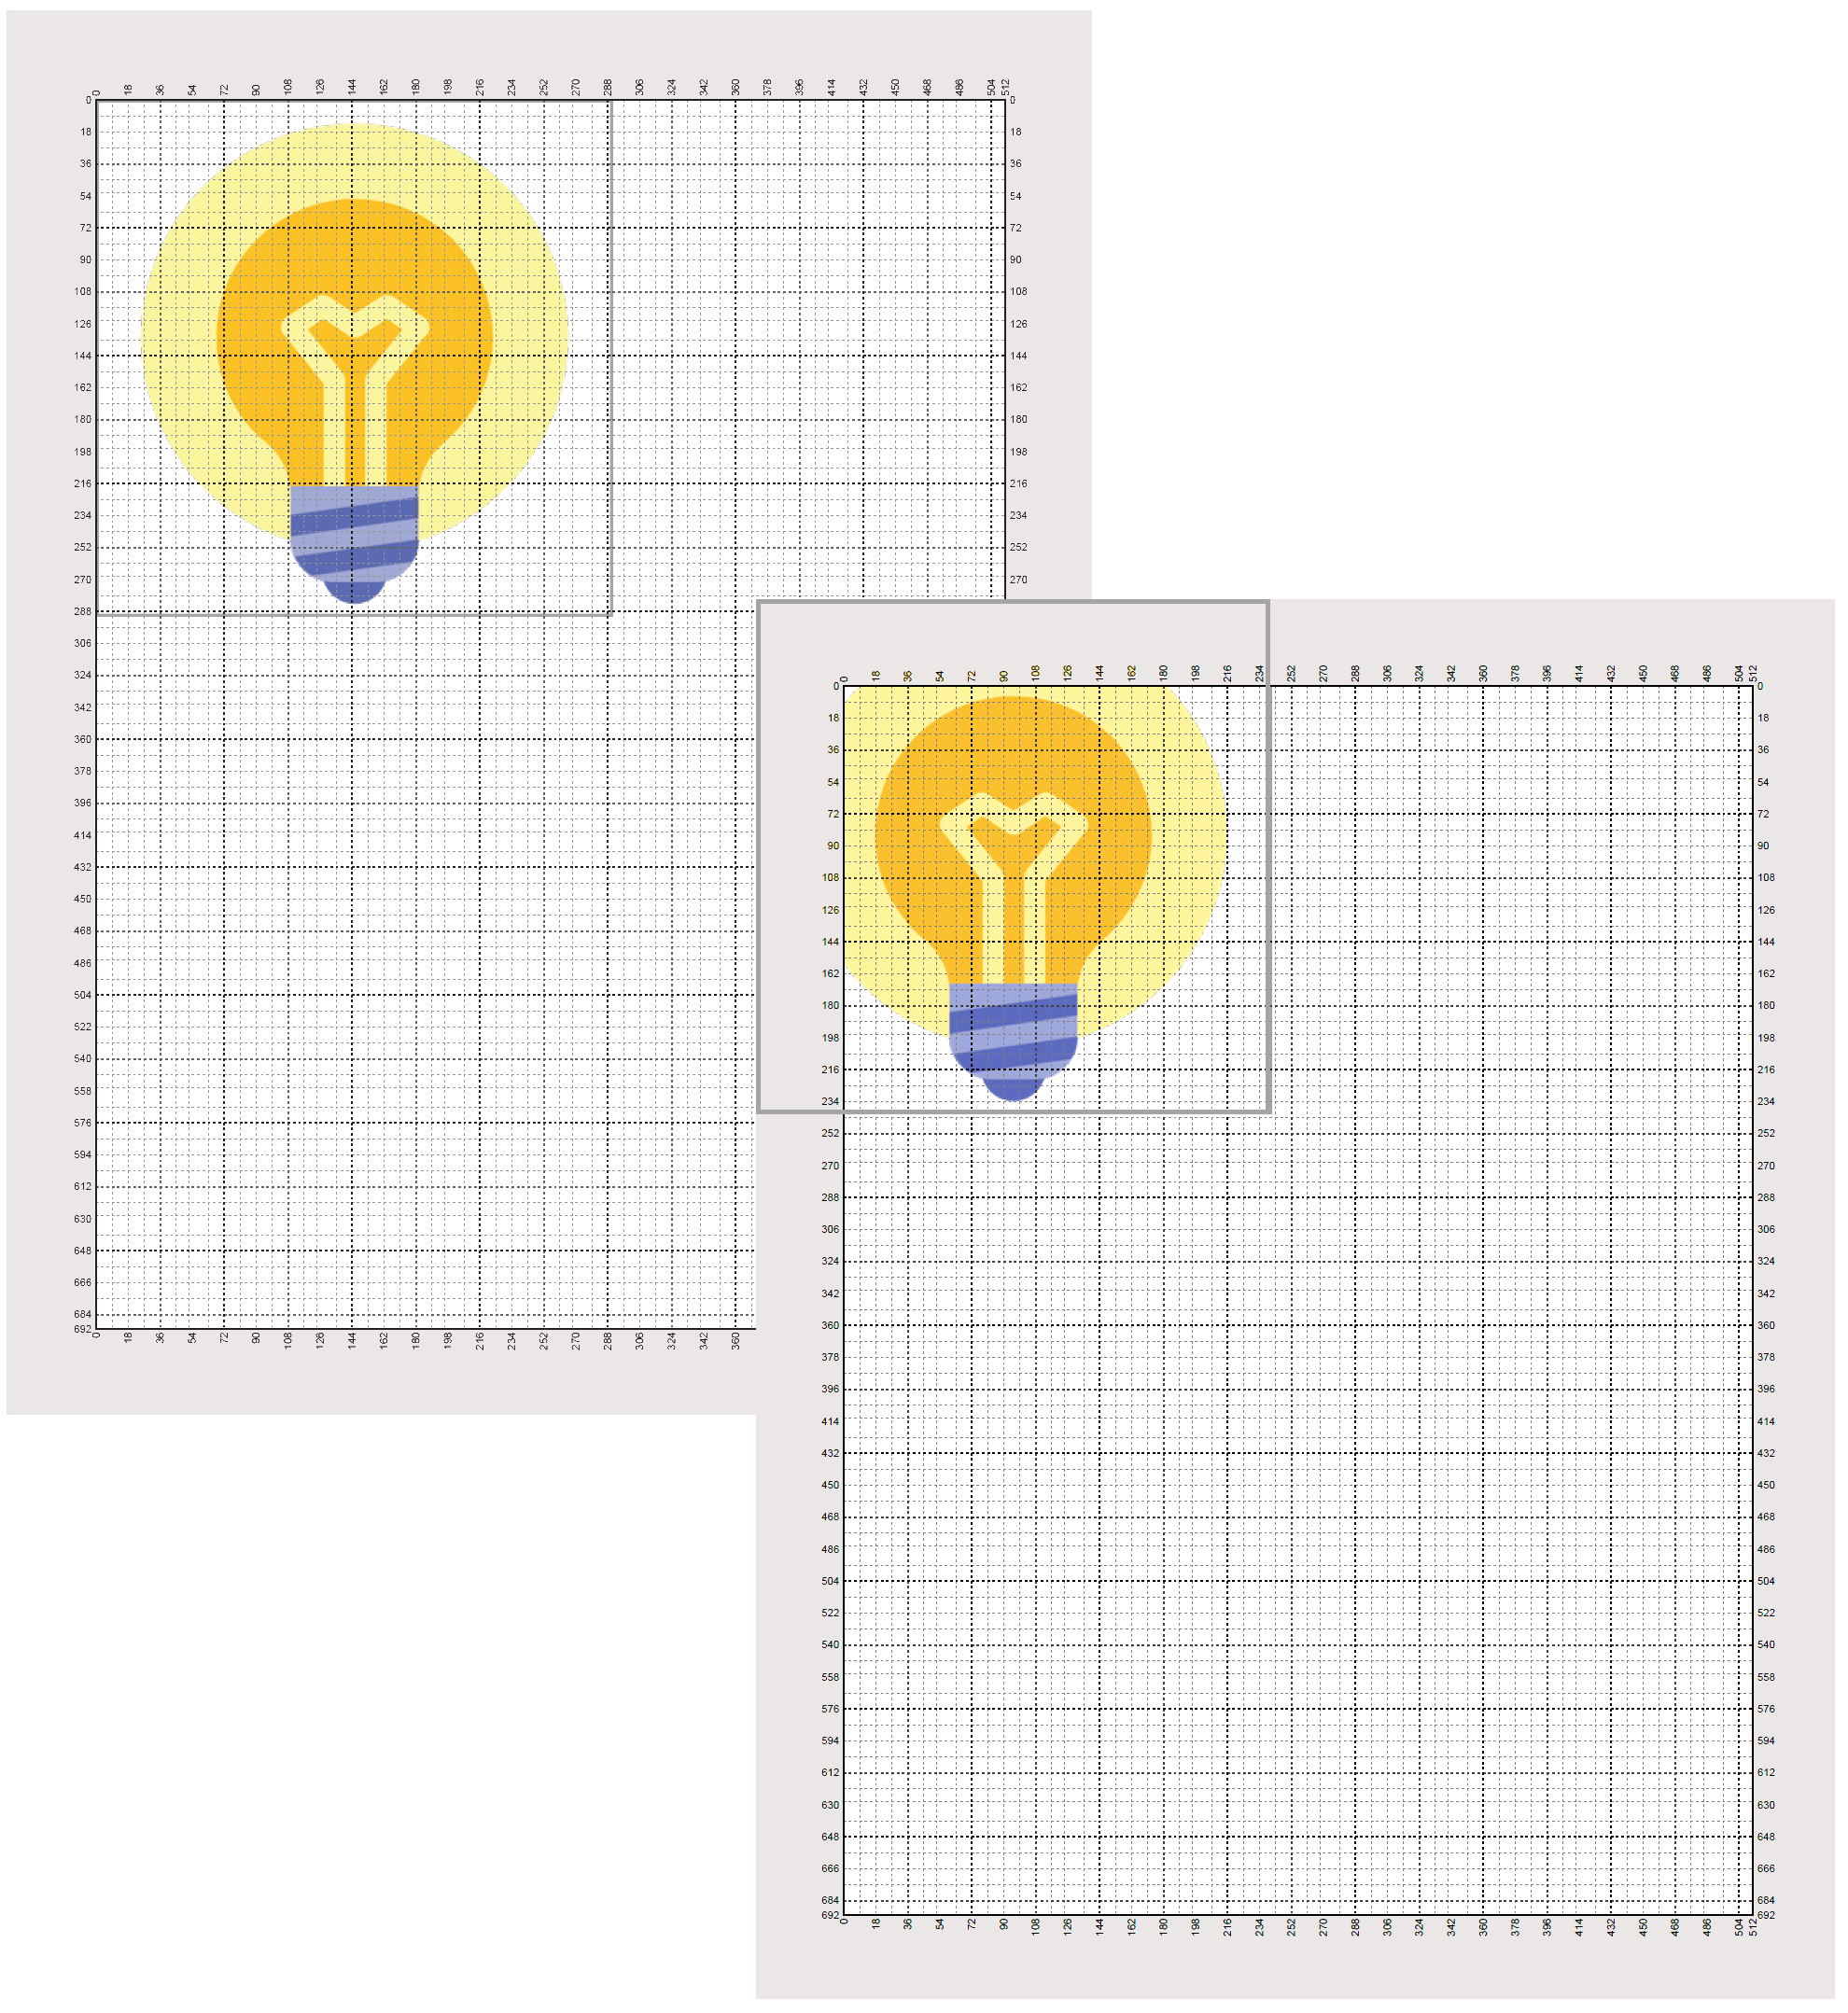
\includegraphics[scale=0.13]{figures/ch2/image-coords-one}\caption{Image centered relative to margin.}\label{mar:Image-marg-relative}
\end{marginfigure}
As an aside, let's consider two more layout examples using our
image. Note the different locations after changing the code in Listing
\ref{lis:Centering-an-image} to the code in Listing \ref{lis:Modifying-Listing-}.
In the first code fragment, the image is positioned on the top right
corner relative to the margin (Figure \ref{mar:Image-marg-relative})
while in the second code fragment the image is positioned relative
to the page (Figure \ref{mar:pg-cent-Image-centered-relative}). 
\begin{marginfigure}
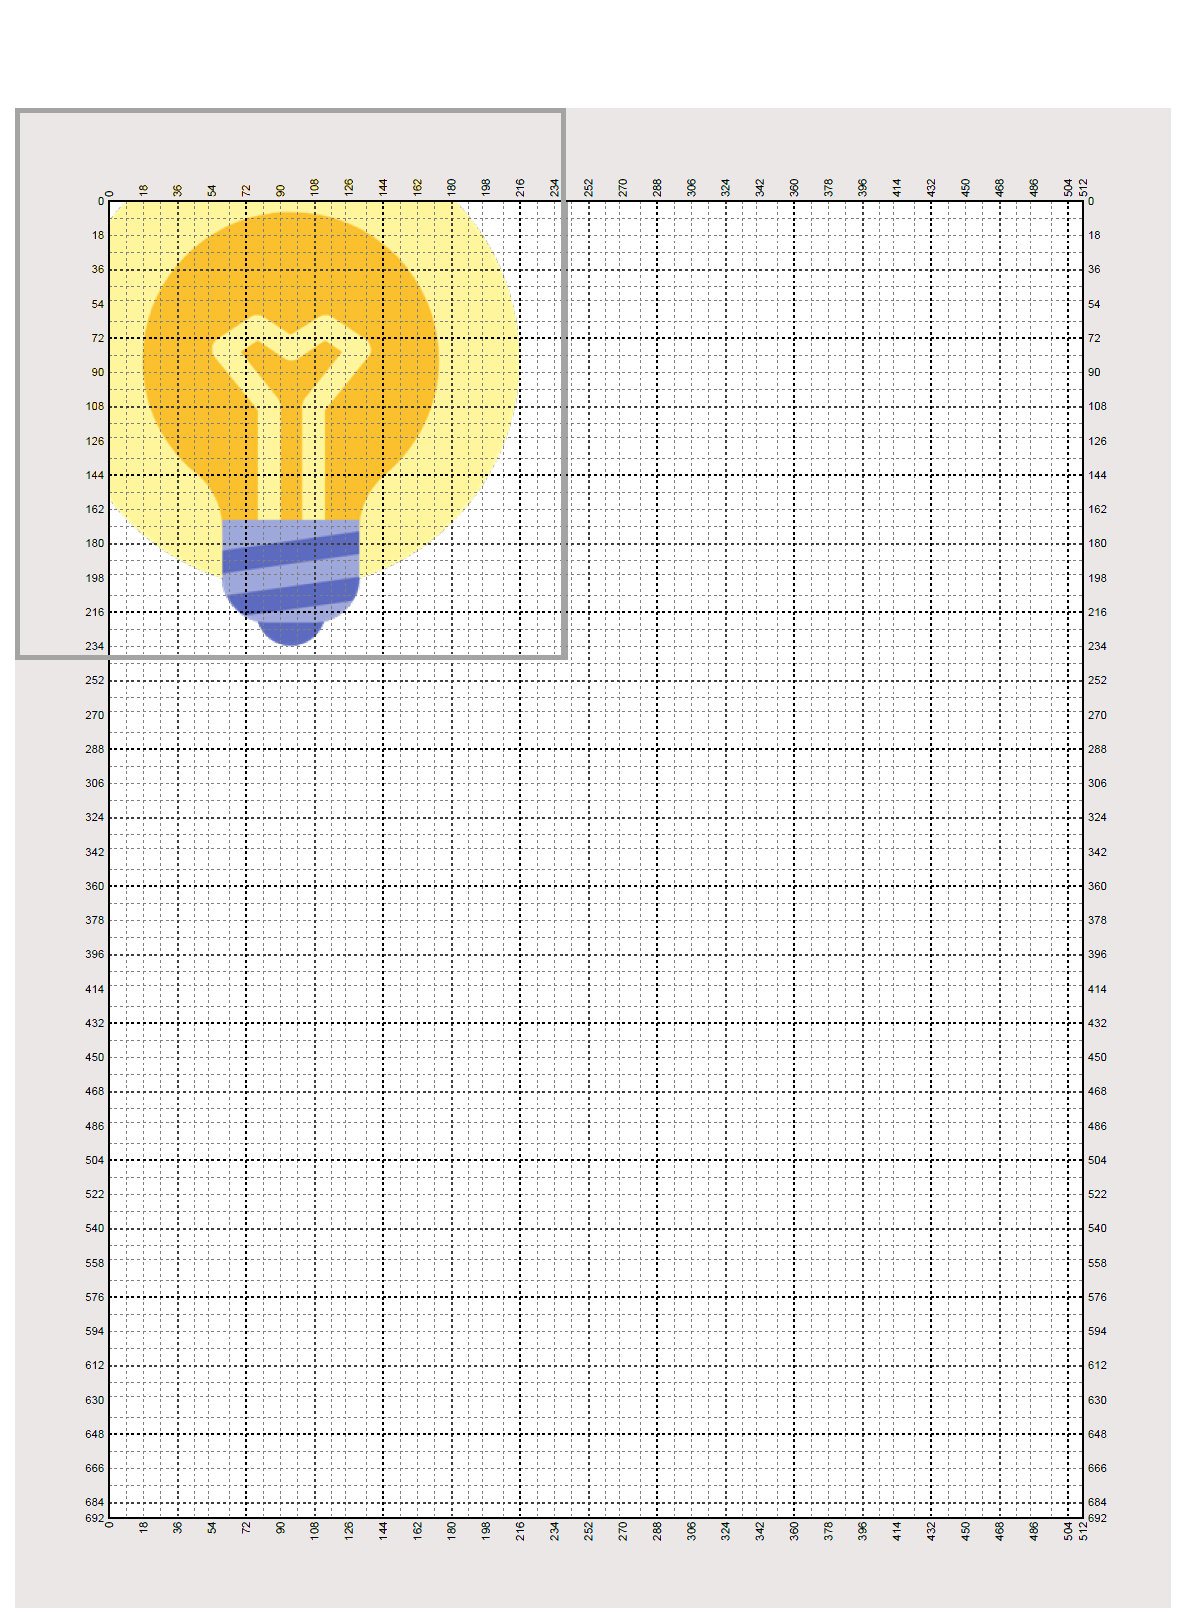
\includegraphics[scale=0.13]{figures/ch2/image-coords-two}\caption{Image centered relative to the page.}\label{mar:pg-cent-Image-centered-relative}
\end{marginfigure}

\bgroup\inputencoding{latin9}
\begin{lstlisting}[caption={Modifying Listing \ref{lis:Centering-an-image} to different image
positions.},label={lis:Modifying-Listing-},basicstyle={\small\ttfamily},breaklines=true]
Document myDoc = new();
Page myPg = new();
myDoc.Pages.Add(myPg);
Image image = new Image(resourcePath + "/idea.png", myPg.Dimensions.RightMargin * -1, myPg.Dimensions.TopMargin * -1);
myPg.Elements.Add(image);
myDoc.Draw(outputPath);

Document myDoc = new();
Page myPg = new();
myDoc.Pages.Add(myPg);
Image image = new Image(resourcePath + "/idea.png", 
  0, 0);
myPg.Elements.Add(image);
myDoc.Draw(outputPath);
\end{lstlisting}
\leavevmode\egroup


\subsection{VAlign and Align Properties}

In Listing \ref{lis:Centering-an-image} we used the \texttt{VAlign}\index{VAlign}
and \texttt{Align}\index{Align} properties after positioning the image to the center
of the page. Because a page element's \texttt{x} and \texttt{y} values are measured from the
upper left corner of the element, we had to use these properties to
complete centering the image (Figure \ref{mar:center-The-image-from}). We can change this behavior using the \texttt{VAlign}\index{VAlign} property.
\begin{figure}
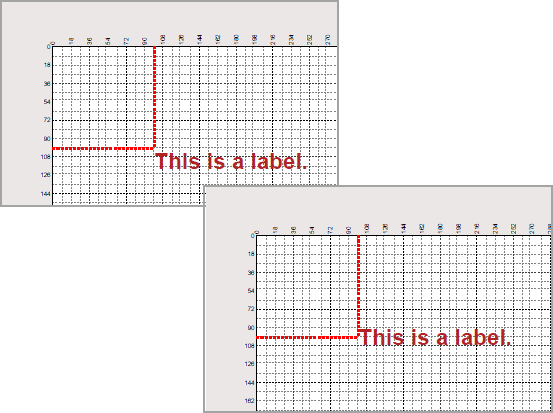
\includegraphics[scale=0.43]{figures/ch2/valign}\caption{Applying VAlign to a Label.}\label{mar:Applying-VAlign-to}
\end{figure}
The \texttt{VAlign}\index{VAlign} property changes the y position to an element's center.
So, for example, if a \texttt{Label} has a \texttt{y} value of 100 and it's
height is 100, then applying the \texttt{VAlign}\index{VAlign} property would change
it's \texttt{y} position to the vertical center of the label (Figure \ref{mar:Applying-VAlign-to}).
 
\subsection{Layout Grid}

Notice that throughout this chapter's example code and figures, we added a layout grid using the \texttt{LayoutGrid}\index{LayoutGrid} class to make the positioning more obvious.\sidenote{I did not include the
code for the layout grid in the listings so you would not be distracted
by irrelevant code.} The \texttt{LayoutGrid}\index{LayoutGrid} page element is extremely
useful for laying out your page when developing your PDF document
and so we briefly consider it here. Listing \ref{lis:ly-grid-Example-using-the}
illustrates using a grid with a circle and rectangle (Figure \ref{fig:layout-gridExample-using-the}).
\begin{figure}
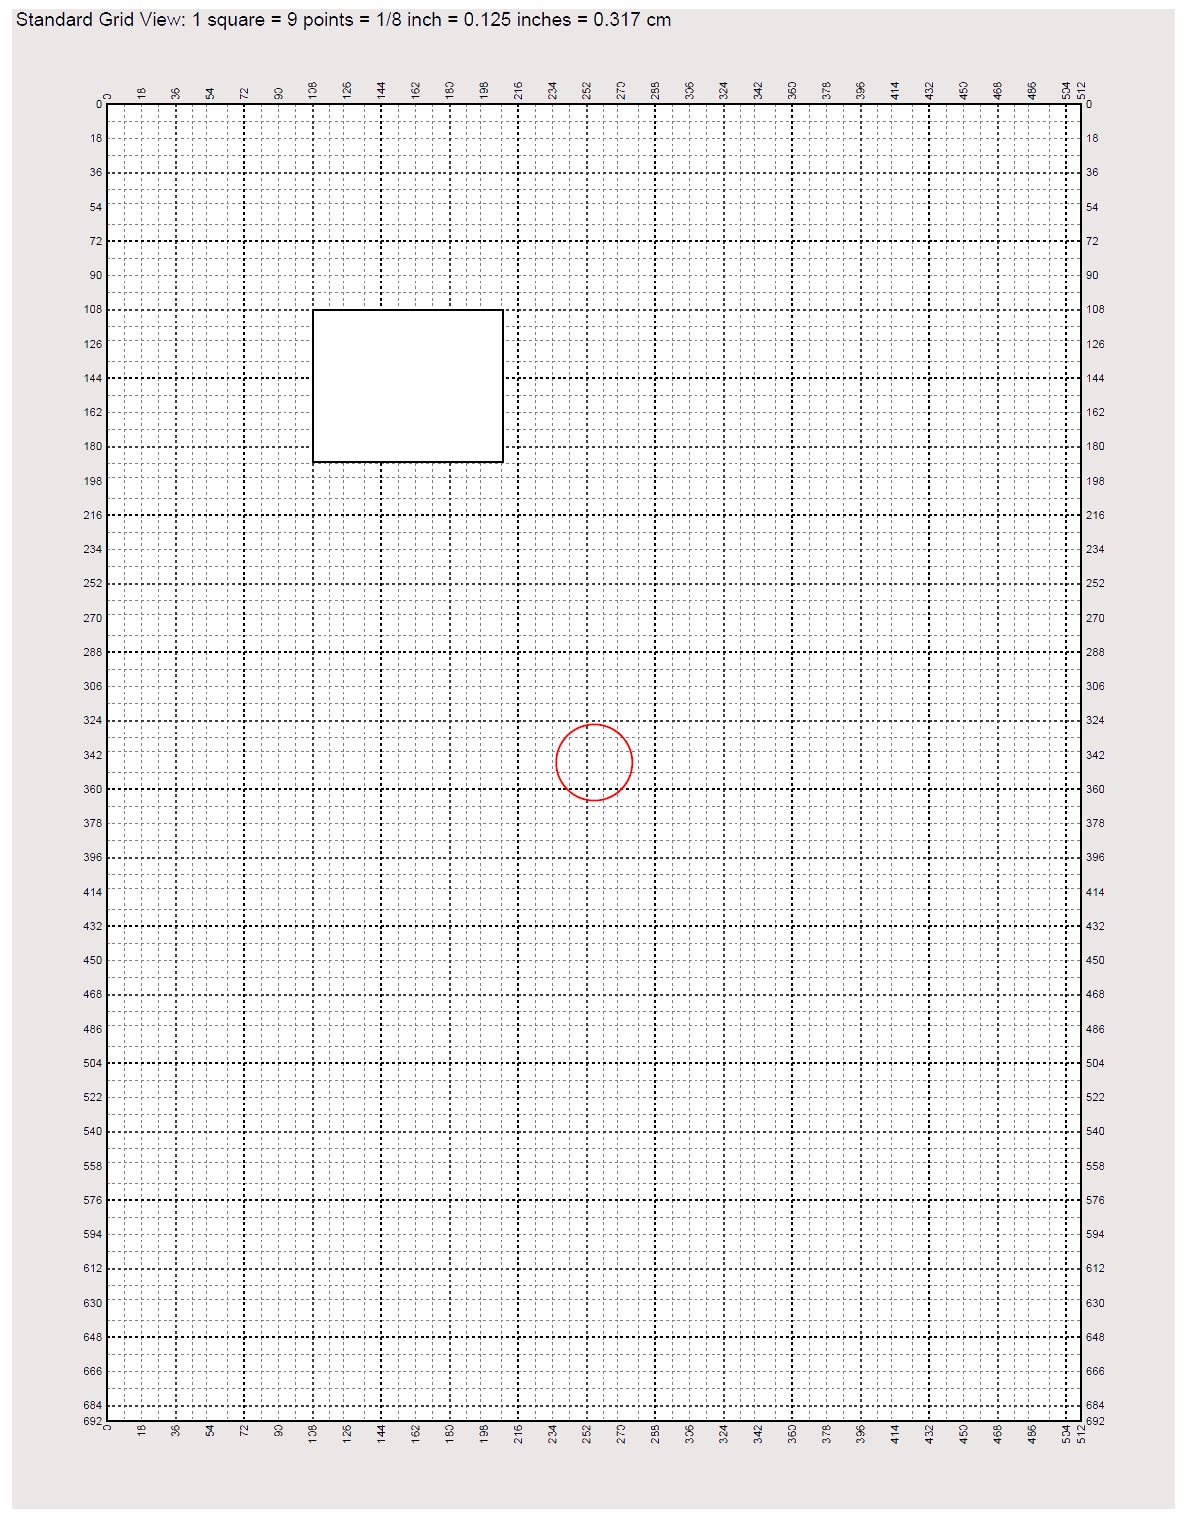
\includegraphics[scale=0.35]{figures/ch2/grid-example}\caption{Using the LayoutGrid class for development.}\label{fig:layout-gridExample-using-the}

\end{figure}
As the resulting PDF document shows, the grid helps in determining
the position of a page's elements.\sidenote{Of course you delete the code for the layout grid after completing
your page's layout.}

\bgroup\inputencoding{latin9}
\begin{lstlisting}[caption={Using the LayoutGrid class for development.},label={lis:ly-grid-Example-using-the},basicstyle={\small\ttfamily},breaklines=true]
using ceTe.DynamicPDF;
using ceTe.DynamicPDF.PageElements;

namespace ChapterExamples.Chapters.ChapterTwo
{
    class LayoutGridExample
    {
        public static void Create(string outputPath)
        {
            Document myDoc = new();
            Page myPg = new();
            myDoc.Pages.Add(myPg);
            float centerX = (myPg.Dimensions.Width - myPg.Dimensions.LeftMargin - myPg.Dimensions.RightMargin) / 2;
            float centerY = (myPg.Dimensions.Height - myPg.Dimensions.TopMargin - myPg.Dimensions.BottomMargin) / 2;
            LayoutGrid layGrd = new();
            layGrd.Type = LayoutGrid.GridType.Standard;
            myPg.Elements.Add(layGrd);
            Rectangle rec = new(108, 108, 100, 80);
            rec.FillColor = RgbColor.White;
            myPg.Elements.Add(rec);
            Circle circle = new(centerX, centerY, 20,20);
            circle.BorderColor = RgbColor.Red;
            myPg.Elements.Add(circle);         
            myDoc.Draw(outputPath);
        }
    }
}
\end{lstlisting}
\leavevmode\egroup

By default, a layout grid is relative to the page's margins. However,
you can change the default by setting the \texttt{IgnoreMargins}\index{IgnoreMargins} property
to \texttt{true}. You can set the layout grid to one of four different
types:
\begin{itemize}
\item \texttt{LayoutGrid.GridType.Decimal}\index{LayoutGrid.GridType.Decimal},
\item \texttt{LayoutGrid.GridType.Metric}\index{LayoutGrid.GridType.Metric},
\item \texttt{LayoutGrid.GridType.Print}\index{LayoutGrid.GridType.Print}, and
\item \texttt{LayoutGrid.GridType.Standard}\index{LayoutGrid.GridType.Standard}.
\end{itemize}
Here I only used the \texttt{Standard} layout grid type, which measured
the grid in points. 

When handling page layout, you must be aware of the dimensions, margins, and other aspects when laying out elements on a page. Try to use relative measurement rather than fixed values. Consider using a \texttt{LayoutGrid} if you need to visualize a page's layout. Now that we have discussed handling a page's dimensions, let's return to adding content to a \texttt{Document}\index{Document} class instance.

\section{HTML Layout}

In addition to using the \texttt{Page} class to add pages to a document, there is another way to quickly add content to your PDF documents using
HTML. The \texttt{HtmlLayout}\index{HtmlLayout} class allows creating a page from HTML.
It supports limited HTML 4 and CSS, although it is not intended for
rendering complex web-pages.\sidenote{The \texttt{HtmlLayout}\index{HtmlLayout} class is intended for simple HTML documents,
for converting complex documents, instead use one of DynamicPdf's
products like Converter or HTML Converter.} The class has six overloaded constructors and allows HTML input from
a Stream, string, or URI. It also has properties for setting its margins,
adding headers and footers, and setting an HTML page's base ref. The
\texttt{HtmlLayout}\index{HtmlLayout} class does not support HTML containing links to
local images. Although the HtmlLayout class does not support local
images, if you have access to a web server, even one in your local
environment, then you can embed images in your HTML and render them.
For example, consider the simple HTML in Listing \ref{lis:HTMl-document-with}.

\bgroup\inputencoding{latin9}
\begin{lstlisting}[caption={HTMl document with simple CSS and image link.},label={lis:HTMl-document-with},basicstyle={\small\ttfamily},breaklines=true]
<html>
<head>
    <style>
        p {
            text-indent: 30px;
            font-family: Arial, Helvetica, sans-serif;
            font-size: 14px;
        }
        body {
            color: darkgreen;
        }
    </style>
</head>
<body>
    <img src="https://www.dynamicpdf.com/images/logo.png" />
    <p>
        Ontinuedcay ethay imeTay avellerTray, ithway ayay ightslay accessionyay ofyay eerfulnesschay.
        eallyRay isthay isyay atwhay isyay eantmay ybay ethay ourthFay imensionDay,
        oughthay omesay eoplepay owhay alktay aboutyay ethay ourthFay imensionDay oday
        otnay owknay eythay eanmay ityay. Ityay isyay onlyyay anotheryay ayway ofyay
        ookinglay atyay imeTay.ereThay isyay onay ifferenceday etweenbay imetay andyay
        anyyay ofyay ethay eethray imensionsday ofyay aceSpay exceptyay atthay ouryay
        onsciousnesscay ovesmay alongyay ityay.utBay omesay oolishfay eoplpay.
    </p>
<-- extra paragraphs snip -->
</body>
</html>
\end{lstlisting}
\leavevmode\egroup

The HTML consists of a simple embedded CSS and the body contains an
image available on the DynamicPDF website. Listing \ref{lis:Using-the-HtmlLayout}
loads the HTML as text and a \texttt{PageInfo}\index{PageInfo} instance to create a new \texttt{HtmlLayout}\index{HtmlLayout}
instance.\sidenote{The \texttt{TextGenerator} class is a utility class in the GitHub
project that reads the HTML into a string from a file.} You then add a header and footer and then create the PDF document (Figure \ref{fig:Using-an-HtmlLayout}).
\begin{figure}

\includegraphics[scale=0.25]{figures/ch2/fig10}\caption{Using an HtmlLayout to create a PDF document.}\label{fig:Using-an-HtmlLayout}
\end{figure}
\bgroup\inputencoding{latin9}
\begin{lstlisting}[caption={Using the HtmlLayout class to create a PDF document.},label={lis:Using-the-HtmlLayout},basicstyle={\small\ttfamily},breaklines=true]
using ceTe.DynamicPDF;
using ChapterExamples.Utility;

namespace ChapterExamples.Chapters.ChapterTwo
{
    public class HtmlLayoutExample
    {
        public static void Create(string outputPath)
        {
            PageInfo layoutPage = new(PageSize.Letter, PageOrientation.Portrait);
            HtmlLayout html = new(TextGenerator.GenerateHtmlWithImg(), layoutPage);
            html.Header.Center.Text = "%%PR%%%%SP%% of %%ST%%";
            html.Header.Center.HasPageNumbers = true;
            html.Header.Center.Width = 200;
            html.Footer.Center.Text = "%%PR%%%%SP(A)%% of %%ST(B)%%";
            html.Footer.Center.HasPageNumbers = true;
            html.Footer.Center.Width = 200;
            Document myDoc = html.Layout();
            myDoc.Draw(outputPath);
        }
    }
}
\end{lstlisting}
\leavevmode\egroup

\section{Adding Document Properties}

Now let's change topics again and switch from discussing page layout  and adding content to a \texttt{Document}\index{Document} instance and instead discuss a document's properties and modifying how that document's properties appear in a PDF reader such as Adobe Acrobat. Listing \ref{lis:ch2-doc-prop-Creating-a-document}
illustrates adding properties to a PDF document. It sets the document's
author, title, creator, and subject. It also adds several keywords
to the document.
\begin{marginfigure}

\includegraphics[scale=0.41]{figures/ch2/fig1}\caption{Document properties dialog.}\label{fig:Document-properties-dialog.}
\end{marginfigure}
 The resulting PDF document will then display the properties, usually
in a dialog box, when queried. For example, Figure \ref{fig:Document-properties-dialog.}
uses Adobe Acrobat to display the PDF document's properties in the
\textbf{Document Properties}\index{Document Properties} dialog box when selecting \textbf{Document
Properties...} in the document's context menu.

\bgroup\inputencoding{latin9}
\begin{lstlisting}[caption={Document level properties.},label={lis:ch2-doc-prop-Creating-a-document},basicstyle={\small\ttfamily},breaklines=true]
using ceTe.DynamicPDF;
using ceTe.DynamicPDF.PageElements;

namespace ChapterExamples.Chapters.ChapterTwo
{
    class DocPagePropsExample
    {
        public static void Create(string outputPath)
        {
            Document myDoc = new();
            myDoc.Title = "DynamicPDF Ch2 Properties Example";
            myDoc.Author = "James Brannan";
            myDoc.Creator = "James Brannan";
            myDoc.Subject = "DynamicpDF Core Suite by Example";
            myDoc.Keywords = "DynamicPDF Book Core Suite Example";
            Page myPg = new();
            Label myLabel = new("Document Properties Example", 50, 50, 200, 50);
            myPg.Elements.Add(myLabel);
            myDoc.Pages.Add(myPg);
            myDoc.Draw(outputPath);
        }
    }
}
\end{lstlisting}
\leavevmode\egroup
\begin{marginfigure}
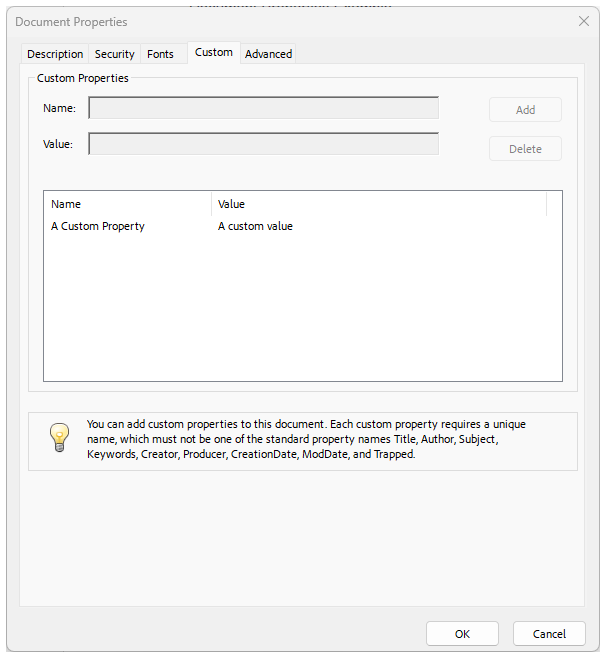
\includegraphics[scale=0.35]{figures/ch2/custom-props}\caption{A custom property.}\label{mar:A-custom-property}
\end{marginfigure}
You can also add custom properties to your PDF document. Modifying Listing \ref{lis:ch2-doc-prop-Creating-a-document} to also include the following code adds a custom property to the resultant
PDF document (Figure \ref{mar:A-custom-property}). {\ttfamily\bgroup\inputencoding{latin9}
\begin{lstlisting}[basicstyle={\small\ttfamily},breaklines=true]
myDoc.CustomProperties.Add("A Custom Property", "A custom value");
\end{lstlisting}
\leavevmode\egroup
}

\section{Viewer Preferences}

A PDF document's initial view depends on how you set the document's
properties.A document may open to a particular page, magnification,
or chose not to display the title. You set a document's viewer preferences
through the \texttt{Document}\index{Document} class's \texttt{ViewerPreferences}\index{ViewerPreferences} class
(Figure \ref{mar:viewer-prefs-Adobe-Reader-display}).
\begin{figure}
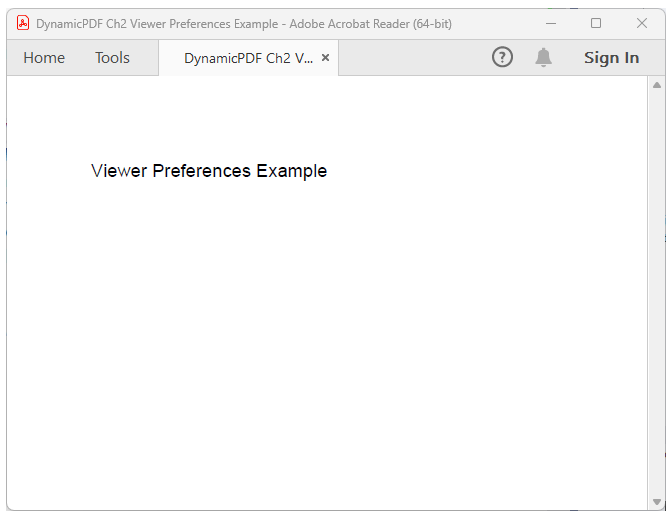
\includegraphics[scale=0.54]{figures/ch2/viewer-prefs}\caption{Adobe Reader display reflecting viewer settings applied by Listing
\ref{lis:Setting-viewer-preferences}.}\label{mar:viewer-prefs-Adobe-Reader-display}
\end{figure}

In Listing \ref{lis:Setting-viewer-preferences} you set the PDF document to center the PDF document in the PDF viewer's window, hide the menubar, display the document title, and to fit in the viewer's window.
\bgroup\inputencoding{latin9}
\begin{lstlisting}[caption={Setting viewer preferences.},label={lis:Setting-viewer-preferences},basicstyle={\small\ttfamily},breaklines=true]
using ceTe.DynamicPDF;
using ceTe.DynamicPDF.PageElements;

namespace ChapterExamples.Chapters.ChapterTwo
{
    class ViewerPrefExample
    {
        public static void Create(string outputPath)
        {
            Document myDoc = new();
            myDoc.Title = "DynamicPDF Ch2 Viewer Preferences Example";
            myDoc.ViewerPreferences.CenterWindow = true;
            myDoc.ViewerPreferences.HideMenubar = true;
            myDoc.ViewerPreferences.DisplayDocTitle = true;
            myDoc.ViewerPreferences.HideToolbar = true;
            myDoc.ViewerPreferences.FitWindow = true;

            Page myPg = new(PageSize.Postcard, PageOrientation.Landscape, 5F);
            Label myLabel = new("Viewer Preferences Example", 50, 50, 200, 50);
            myPg.Elements.Add(myLabel);
            myDoc.Pages.Add(myPg);
            myDoc.Draw(outputPath);
        }
    }
}
\end{lstlisting}
\leavevmode\egroup

Other viewer preference properties\index{viewer preference properties} include \texttt{Duplex}, \texttt{HideWindowUI},
\texttt{NonFullScreenPageMode}, \texttt{NoPrintScaling}, \texttt{NumberOfCopies},
\texttt{PickTrayByPdfSize}, \texttt{PrintArea}, \texttt{PrintClip},
\texttt{PrintPageRange}, \texttt{RightToLeft}, \texttt{ViewArea},
and \texttt{ViewClip}. 

\section{Summary}

In this chapter, you learned how to create a PDF document using the
\texttt{Document} object. You then added pages to that document using
the \texttt{Page} class. Next you learned how to size a page and create
margins for that page using the \texttt{PageDimensions} class. Of
course, there are built-in page sizes such as \texttt{Envelope10},
\texttt{Letter}, and \texttt{Legal}, and the \texttt{PageSize} class
abstracts these page sizes. 

After building a document with pages, we then discussed the coordinate
system and how to properly layout document pages.\sidenote{Remember, always try to use relative measurements rather than hard
values.} As you saw, a letter ($8.5\times11$) page is 612 points wide and
792 points high, where the coordinates are from top to bottom and
left to right.\sidenote{Do not forget to consider the margin in your layout calculations.}
We then used our understanding of coordinates to center circles and
an image on a document's page. After discussing creating and laying
out a document using coordinates we used the \texttt{HtmlLayout} class
to easily create an PDF document from HTML. Of course, the capabilities
of this class are limited compared to DynamicPDF's HtmlConverter and
Converter applications, so if using HTML of any complexity you should
probably use one of those applications. However the HtmlLayout class
is a quick shortcut to creating a PDF document if you know HTML.

We then discussed setting a document's properties and also discussed viewer preferences. Setting a document’s properties provides
important metadata about that document. Viewer preferences allow customizing
how a PDF reader displays and prints a document. Both topics are
important for setting a document's properties or for setting how the
document appears in a PDF reader.

In the next chapter, you learn how to apply templates to your
PDF documents and how to break your documents into sections. A template
allows applying elements to every element on a page without requiring you to create new elements for each page; the template handles that for you. Sections divide a document into sections, grouping important information logically.
You can apply templates to a document or a document’s
sections. After learning about templates and sections you will then be
able to create PDF documents with a consistent appearance between
pages and ensure those pages have a logical organization.

\color{white}
\chapter{Templates and Sections}\label{chap:Templates-and-Document}
\color{black}
\BgThispage
\vspace{8.0em}
\lettrine[lines=2,lhang=0.1]{I}{n} the previous chapter, you learned how to add pages to a document and how to precisely lay out a document's
pages using a PDF's coordinates. In this chapter, we build upon that
knowledge by learning how to create pages with consistent formatting
and sectioning. DynamicPDF Core Suite allows separating documents
into sections. It also allows applying a template to pages to provide
consistent formatting. In this chapter you learn to do both.

Templates add elements to all pages or sections of a document. Core
Suite provides three template types: \texttt{Template}\index{Template}, \texttt{EvenOddTemplate},
and \texttt{HeaderFooterTemplate}. An \texttt{EvenOddTemplate} adds
page elements to every even or odd page in a section or document,
while a \texttt{HeaderFooterTemplate} adds elements to a page's header
and footer. Elements added to a template are, by default, positioned
behind a page's content; however, if you assign a template to a \texttt{Document}\index{Document}
instance's \texttt{StampTemplate} property, then the template positions
its elements above a page's content.\marginnote{The listing in this chapter refer to the code DocumentExampleGenerator.Generate(doc);.
The method simply generates and adds five \texttt{Page} instances
to a \texttt{Document} instance. Find this class in the book's associated
GitHub project.} 

DynamicPDF Core Suite also supports adding sections to PDF documents.
When sectioning a PDF, you can apply different templates to different
sections and change page numbering for each section. 

In this chapter, you will gain practical knowledge on applying templates
to your PDF documents and dividing your documents into sections.

\section{Applying Templates}

Use a \texttt{Template}\index{Template} to apply page elements to every page in a
document or section, thus making a template extremely useful when
creating documents requiring a consistent appearance. It also saves you
from adding the same page elements to multiple pages if they do not
change between pages, as you add the page elements once to the template and they are reused. 

You apply Templates to your PDF using the \texttt{Document}\index{Document} class's
\texttt{Template}\index{Template} property. After setting a template, all page elements
in the \texttt{Template}\index{Template} instance's \texttt{Elements}\index{Elements} collection 
appear in the background of the other PDF content.\sidenote{See the \texttt{StampTemplate}\index{StampTemplate} property for placing elements in the
foreground.} There are three types of templates: \texttt{Template}\index{Template}, \texttt{EvenOddTemplate}\index{EvenOddTemplate},
and \texttt{HeaderFooterTemplate}\index{HeaderFooterTemplate}. The \texttt{EvenOddTemplate}\index{EvenOddTemplate} applies
elements differently depending on whether a page is even or odd, while
the \texttt{HeaderFooterTemplate}\index{HeaderFooterTemplate} adds elements to a header and footer.
The \texttt{Template}\index{Template} class is the parent class of the other two templates
and lacks the specialized functionality of the other two classes. But the class is still useful independently of the other two classes for adding a template to a document.
\subsection{Template Property}
Let's first consider an ordinary template. In Listing \ref{lis:Adding-a-template}
you add a template to a PDF document. After generating some sample
pages using the \texttt{DocumentExampleGenerator} class, you create
a new \texttt{Template}\index{Template} instance. You then add two rectangles, an image,
and a label to the \texttt{Template}\index{Template} instance's \texttt{Elements}\index{Elements}
collection. After adding the elements to the template, you add the
template to the \texttt{Document}\index{Document} instance's \texttt{Template}\index{Template} property.
\begin{marginfigure}

\includegraphics[scale=0.25]{figures/ch3/fig7}\caption{Templates adds consistent formatting.}\label{fig:template-formatting}
\end{marginfigure}
Note that you also add a \texttt{PageNumberingLabel}\index{PageNumberingLabel} element to the
template. We discuss more on page numbering in Chapter \ref{sec:Page-Numbering-Labels};
however, know that here it adds a label who's value displays the current page and 
total pages. You then add the elements to the template and the template
to the document (Figure \ref{fig:tmpl-Applying-a-template}).
\begin{figure}

\includegraphics[scale=0.30]{figures/ch3/fig1}\caption{Applying a template to a five page PDF document.}\label{fig:tmpl-Applying-a-template}
\end{figure}

\bgroup\inputencoding{latin9}
\begin{lstlisting}[caption={Adding a template to a PDF document.},label={lis:Adding-a-template},basicstyle={\small\ttfamily},breaklines=true]
using ceTe.DynamicPDF;
using ceTe.DynamicPDF.PageElements;
using ChapterExamples.Utility;

namespace ChapterExamples.Chapters.ChapterThree
{
    public class TemplateExample
    {
        public static void Create(string resourcePath, string outputPath)
        {
            Document doc = new();
            DocumentExampleGenerator.Generate(doc);
            Page pg = doc.Pages[0];
            Template tmp = new();

            float hgt = pg.Dimensions.Height;
            float x = -pg.Dimensions.LeftMargin;
            float y = -pg.Dimensions.TopMargin;
            float wdt = pg.Dimensions.Width;

            Rectangle rec = new(x,y, 20, hgt);
            rec.FillColor = RgbColor.Navy;
            rec.BorderColor = RgbColor.Navy;

            Rectangle bkRec = new(x, y, wdt, hgt);
            bkRec.FillColor = RgbColor.LightSkyBlue;
            bkRec.BorderColor = RgbColor.LightSkyBlue;

            Image img = new(resourcePath + "logo.png", x+10, y+5, .3F);

            Label lbl = new("DRAFT", 125, 300, 400, 0);
            lbl.TextColor = RgbColor.Red;
            lbl.TextOutlineColor = RgbColor.Black;
            lbl.FontSize = 90;

            PageNumberingLabel pgNm = new PageNumberingLabel("%%CP%% of %%TP%%", 0, hgt+(y *2), wdt+(x*2), 50);
            pgNm.Align = TextAlign.Center;

            tmp.Elements.Add(bkRec);
            tmp.Elements.Add(rec);
            tmp.Elements.Add(img);
            tmp.Elements.Add(lbl);
            tmp.Elements.Add(pgNm);
            doc.Template = tmp;
            
            doc.Draw(outputPath);
        }
    }
}
\end{lstlisting}
\leavevmode\egroup
Note that in Listing \ref{lis:Adding-a-template} the background rectange, rectangle, image, label, and page numbering label are all added to the template's elements array and not a page's. The template is then added to the document. By adding the template to the document, you ensure that every page in the document will have the template applied to the page. The result is a PDF document with consistent appearance across its pages.

As Figure \ref{fig:tmpl-Applying-a-template} illustrates, the template
is applied to every page in the PDF document. The template adds a
background color, a logo intended as letterhead, page numbering, and
finally adds "DRAFT" to each page.\sidenote{Later you will see the \texttt{TextWatermark}\index{TextWatermark} and \texttt{ImageWatermark}\index{ImageWatermark}
classes to create "true" watermarks.} Don't worry if you do not fully understand page elements and how
to add them to your document yet, as we discuss them in Chapter \ref{chap:Page-Elements--text} and Chapter \ref{chap:Page-Elements--graphics}. But as Figure \ref{fig:tmpl-Applying-a-template}
illustrates, because we used a template, the document is consistent
across pages and the code is also less than if the same elements had to be added to each page.
\subsection{Stamp Template Property}
In Figure \ref{fig:tmpl-Applying-a-template}, notice the template's
elements appear behind the page's elements. Placing elements behind
a page's content is standard for all three templates. However, you can change this behavior for a document by setting the
template to the Document instance's \texttt{StampTemplate}\index{StampTemplate} property
rather than its \texttt{Template}\index{Template} property. All page elements of the
template will then appear in the foreground, in front of the page's
elements.
\begin{marginfigure}

\includegraphics[scale=0.30]{figures/ch3/fig8}\caption{Stamp Template places elements in foreground.}\label{fig:template-formatting}
\end{marginfigure}
In Listing \ref{lis:forground-Using-a-stamp} we create a template
and then assign it to a document's \texttt{StampTemplate}\index{StampTemplate} property.
In our example, this creates a PDF where half the page is obscured
by the template because it places the template's elements in the document's
foreground (Figure \ref{fig:Applying-a-stamp}). Of course obscuring
half a page is not ideal design, but it gets the point across.

One thing to note, is that we set the \texttt{StampTemplate}\index{StampTemplate} instance
to the document's \texttt{StampTemplate}\index{StampTemplate} not the \texttt{Template}\index{Template}
in Listing \ref{lis:forground-Using-a-stamp}. If we wished, we could
have also applied a standard template to the document where the template's
elements appear in the background by setting the template to the document's
\texttt{Template}\index{Template} property.
\begin{figure}

\includegraphics[scale=0.35]{figures/ch3/fig2}\caption{Applying a stamp template to a five page PDF document.}\label{fig:Applying-a-stamp}
\end{figure}

\bgroup\inputencoding{latin9}
\begin{lstlisting}[caption={Using a stamp template.},label={lis:forground-Using-a-stamp},basicstyle={\small\ttfamily},breaklines=true]
using ceTe.DynamicPDF;
using ceTe.DynamicPDF.PageElements;
using ChapterExamples.Utility;

namespace ChapterExamples.Chapters.ChapterThree
{
    public class StampTemplateExample
    {
        public static void Create(string resourcePath, string outputPath)
        {
            Document doc = new();
            DocumentExampleGenerator.Generate(doc);
       Pages pg = doc.Pages[0];
            Template tmp = new();

            float hgt = pg.Dimensions.Height/3;
            float wdt = pg.Dimensions.Width;
            float x = -pg.Dimensions.LeftMargin;
            float y = -pg.Dimensions.TopMargin;

            Rectangle rec = new(x, y, 20, hgt);
            rec.FillColor = RgbColor.Navy;
            rec.BorderColor = RgbColor.Navy;

            Rectangle bkRec = new(x, y, wdt, hgt);
            bkRec.FillColor = RgbColor.LightSkyBlue;
            bkRec.BorderColor = RgbColor.LightSkyBlue;

            Label lbl = new("Test.", 200, 300, 200, 0);
            lbl.TextColor = RgbColor.Red;
            lbl.TextOutlineColor = RgbColor.Black;
            lbl.FontSize = 90;

            Image img = new(resourcePath + "logo.png", x + 10, y + 5, .3F);

            tmp.Elements.Add(bkRec);
            tmp.Elements.Add(rec);
            tmp.Elements.Add(img);
            tmp.Elements.Add(lbl);
            doc.StampTemplate = tmp;
            doc.Draw(outputPath);
        }
    }
}
\end{lstlisting}
\leavevmode\egroup


\subsection{Even/Odd Templates}

An \texttt{EvenOddTemplate}\index{EvenOddTemplate} applies page elements to a template depending
on whether the page is even or odd. Instead of having a single \texttt{Elements}\index{Elements}
collection, like the \texttt{Template}\index{Template} class, it has an \texttt{EvenElements}\index{EvenElements}
collection and an \texttt{OddElements}\index{OddElements} collection. You add page elements
to either collection depending on whether you wish the element to
appear on the odd page or the even page. Listing \ref{lis:Applying-diffent-template}
illustrates.

Listing \ref{lis:Applying-diffent-template} recreates a common numbering
strategy (this book's strategy, in fact) where odd pages place the
book's title and page number on the right while even pages place the
author's name and page number on the left (Figure \ref{fig:Applying-an-even/odd}). 

\bgroup\inputencoding{latin9}
\begin{lstlisting}[caption={Applying an EvenOddTemplate to a PDF document.},label={lis:Applying-diffent-template},basicstyle={\small\ttfamily},breaklines=true]
using ceTe.DynamicPDF;
using ceTe.DynamicPDF.PageElements;

namespace ChapterExamples.Chapters.ChapterThree
{
    public class EvenOddTemplateExample
    {
        public static void Create(string outputPath)
        {
            Document doc = new();
            EvenOddTemplate tmp = new EvenOddTemplate();
            tmp.EvenElements.Add(new PageNumberingLabel("%%SP%%  James A Brannan", 0, 0, 512, 12, Font.Helvetica, 12, TextAlign.Left));
            tmp.OddElements.Add(new PageNumberingLabel("DynamicPDF Core Suite by Example  %%SP%%", 0, 0, 500, 12, Font.Helvetica, 12, TextAlign.Right));
            doc.Template = tmp;

            for (int i = 0; i < 7; i++)
            {
                doc.Pages.Add(new Page(PageSize.Letter));
            }

            doc.Draw(outputPath);
        }
    }
}
\end{lstlisting}
\leavevmode\egroup

Each page has a header, placing the book's title and page number to
the right on odd pages. Even pages place the author's name and page
number on the left (Figure \ref{fig:Applying-an-even/odd}).

\begin{figure}


\includegraphics[scale=0.38]{figures/ch3/fig3}\caption{Applying an even/odd template to a PDF document.}\label{fig:Applying-an-even/odd}
\end{figure}


\subsection{Header/Footer Templates}

A \texttt{HeaderFooterTemplate}\index{HeaderFooterTemplate} places header or footer text on a
page's header or footer and allows text to be placed on the left,
center, or right using an instance of the \texttt{HeaderFooterText}\index{HeaderFooterText}
class. The \texttt{HeaderFooterTemplate}\index{HeaderFooterTemplate} has a \texttt{FooterCenter}\index{FooterCenter},
\texttt{FooterLeft}\index{FooterLeft}, \texttt{FooterRight}\index{FooterRight}, \texttt{HeaderCenter}\index{HeaderCenter},
\texttt{HeaderLeft}\index{HeaderLeft}, and \texttt{HeaderRight}\index{HeaderRight} property for placing
the text. This placement is only for text. Custom elements
such as page numbering require you to lay out the template's elements
as you would an instance of the \texttt{Template}\index{Template} class.

In Listing \ref{lis:Applying-headers-and}, you add header text to
a page's left and footer text to its center. You also add page numbering
to header, only you place the page numbering label manually
by determining the proper coordinates. The end result is the produced
PDF has a header and footer on each page (Figure \ref{fig:Applying-a-header}).
\begin{marginfigure}

\includegraphics[scale=0.30]{figures/ch3/fig6}\caption{Applying a header and footer to a PDF document.}\label{fig:Applying-a-header}
\end{marginfigure}

\bgroup\inputencoding{latin9}
\begin{lstlisting}[caption={Using the HeaderFooterTemplate class.},label={lis:Applying-headers-and},basicstyle={\small\ttfamily},breaklines=true]
using ceTe.DynamicPDF;
using ceTe.DynamicPDF.PageElements;
using ChapterExamples.Utility;

namespace ChapterExamples.Chapters.ChapterThree
{
    public class HeaderFooterExample
    {
        public static void Create(string outputPath)
        {
            Document doc = new();
            DocumentExampleGenerator.Generate(doc);
            Page pg = doc.Pages[0];
            float x = pg.Dimensions.Width - pg.Dimensions.RightMargin * 2;
            float y = -pg.Dimensions.TopMargin;

            HeaderFooterTemplate header = new HeaderFooterTemplate();
            HeaderFooterText leftText = new HeaderFooterText("DynamicPDF Core Suite by Example");
            leftText.Font = Font.Helvetica;
            leftText.FontSize = 12;
            header.HeaderLeft = leftText;
            header.FooterCenter = new HeaderFooterText("This is a draft...");
            PageNumberingLabel pglb = new("%%CP%% of %%TP%%", x, y, 100, 50, Font.Helvetica, 12, TextAlign.Left);
            pglb.VAlign = VAlign.Center;
            header.Elements.Add(pglb);
            doc.Template = header;
            doc.Draw(outputPath);
        }
    }
}
\end{lstlisting}
\leavevmode\egroup

\section{Sectioning Documents}

Now that we examined how to use templates for consistent layout
and appearance between a document's pages, let's move to examining
how to use sectioning to logically organize a PDF document. Most documents
with more than a few pages are divided into sections, chapters, or
some other sectioning, signifying changes in topics. When creating
a PDF, Core Suite supports document sectioning using the \texttt{Document}
class's \texttt{Sections}\index{Document Sections} collection. 
When you add sections to a document, you add them at the same time you add pages, alternating between adding the desired pages in a section and then adding a new section, and then repeating (Figure \ref{fig:sections-linear}). Each section can change the PDF viewer's numbering and can also change
the template applied to the pages in that section, as Listing \ref{lis:Applying-sectioning-to}
illustrates. \marginnote{A section's page numbering is for the PDF Reader's benefit, not for
displaying using a template.}

A \texttt{Document} class instance adds pages to the document. Then,
when ready to create a section, you begin a new section. You then
add more pages and, if applicable, add another new section. Repeat
creating pages and creating sections as many times as needed. 

In Listing
\ref{lis:Applying-sectioning-to}, you create a document with three
sections using the document sections \texttt{Begin} method. This method
also takes a page numbering style and optional text. The PDF Reader's
toolbar then displays the page numbering and text for that section
(Figure \ref{fig:final-Example-of-applying}).\begin{marginfigure}

\includegraphics[scale=0.40]{figures/ch3/fig9}\caption{Add sections as you add pages.}\label{fig:sections-linear}
\end{marginfigure}

\bgroup\inputencoding{latin9}
\begin{lstlisting}[caption={Applying sectioning to a PDF document.},label={lis:Applying-sectioning-to},basicstyle={\small\ttfamily},breaklines=true]
using ceTe.DynamicPDF;
using ceTe.DynamicPDF.PageElements;

namespace ChapterExamples.Chapters.ChapterThree
{
    public class SimpleTemp
    {
        public static void Create(string outputPath)
        {
            Document doc = new Document();
            Template tmp = new Template();
            tmp.Elements.Add(new PageNumberingLabel("%%SP%% of %%ST%%", 0, 680, 512, 12, Font.Helvetica, 12, TextAlign.Center));
            doc.Sections.Begin(NumberingStyle.RomanLowerCase);
            doc.Pages.Add(new Page()); 
            doc.Sections.Begin(NumberingStyle.Numeric, tmp);
            doc.Pages.Add(new Page());
            doc.Pages.Add(new Page());
            doc.Sections.Begin(NumberingStyle.RomanLowerCase, "Last Section - ", tmp);
            doc.Pages.Add(new Page());
            doc.Pages.Add(new Page());
            doc.Draw(outputPath);
        }
    }
}
\end{lstlisting}
\leavevmode\egroup

\begin{figure}


\includegraphics[scale=0.38]{figures/ch3/fig4}\caption{Applying a header/footer template to a PDF document.}\label{fig:Applying-a-header/footer}
\end{figure}


\subsection{Omitting Sections}

When applying templates to a section - or the entire document - you
can omit applying a template to specific pages. By default, a page
sets both the document and section template if either has a template.
To change this behavior, set a page's \texttt{ApplyDocumentTemplate}\index{ApplyDocumentTemplate} or \texttt{ApplySectionTemplate}\index{ApplySectionTemplate}
property to \texttt{False} to disable the template for that individual page.
For example, in Listing \ref{lis:Omitting-template-from} the second
page is not added to the template and so is not added to the created
PDF document for that page.

\bgroup\inputencoding{latin9}
\begin{lstlisting}[caption={Omitting template from a single page of a document.},label={lis:Omitting-template-from},basicstyle={\small\ttfamily},breaklines=true]
public static void Create(string outputPath)
{
  Document doc = new Document();
  Template tmp = new Template();
  doc.Template = tmp;
  tmp.Elements.Add(new PageNumberingLabel("%%SP%% of %%ST%%", 0, 680, 512, 12, Font.Helvetica, 12, TextAlign.Center));
  doc.Pages.Add(new Page());
  doc.Pages.Add(new Page());
  doc.Pages[1].ApplyDocumentTemplate = false;
  doc.Pages.Add(new Page());
  doc.Draw(outputPath);
}
\end{lstlisting}
\leavevmode\egroup

You can also limit page output for an individual document section, as Listing
\ref{lis:Omitting-template-from-1} illustrates.

\bgroup\inputencoding{latin9}
\begin{lstlisting}[caption={Omitting template from a section page.},label={lis:Omitting-template-from-1},basicstyle={\small\ttfamily},breaklines=true]
public static void Create2(string outputPath)
{
    Document doc = new Document();
    Template tmp = new Template();
    tmp.Elements.Add(new PageNumberingLabel("%%SP%% of %%ST%%", 0, 680, 512, 12, Font.Helvetica, 12, TextAlign.Center));
    doc.Sections.Begin(NumberingStyle.Numeric, tmp);
    doc.Pages.Add(new Page());
    doc.Sections.Begin(NumberingStyle.Numeric, tmp);
    doc.Pages.Add(new Page());
    doc.Pages.Add(new Page());
    doc.Pages.Add(new Page());
    doc.Pages[2].ApplySectionTemplate = false;
    doc.Draw(outputPath);
}
\end{lstlisting}
\leavevmode\egroup


\section{A Complete Example}

Now that we know how to add templates to a document and how to section
a document, let's create a complete example illustrating both concepts.
Although we have not discussed page elements yet, to create a reasonable
example, we include them in this example. Don't worry though, we cover
these page elements in subsequent chapters. In this section we create
a hypothetical employee handbook consisting of a cover page, two sections,
and an addendum. Despite this section's title, we omit considerable
formatting code and only illustrate creating the document, its sections,
and applying templates. Moreover, you already understand the code behind creating
a template, so there is no reason to repeat it here. However, the
GitHub project has the complete code for this example, including the
code that adds and positions each template's elements. 

Listing \ref{lis:A-PDF-document} creates a sample document with a
cover page, two sections, and a third section as an addendum. First,
you make a cover page that applies a template to the cover page. Next,
you create two sections, using different templates for each section.
Finally, you create another section, but instead of applying numeric
page numbering, you apply Roman numerals to indicate it's an addendum
to the main document. The result is the PDF document in Figure \ref{fig:final-Example-of-applying}.

\bgroup\inputencoding{latin9}
\begin{lstlisting}[caption={A PDF document with multiple sections.},label={lis:A-PDF-document},basicstyle={\small\ttfamily},breaklines=true]
using ceTe.DynamicPDF;
using ceTe.DynamicPDF.PageElements;
using ChapterExamples.Utility;

namespace ChapterExamples.Chapters.ChapterThree
{
    public class SectionDifferentTemp
    {
        public static void Create(string resourcePath, string outputPath)
        {
            Document doc = new();
            Page cvrPg = new();
           
           Template tmpCvr = SectionDifferentTemp.CreateCoverTemplate(resourcePath, cvrPg);
           doc.Sections.Begin(NumberingStyle.None, "Worker's Handbook", tmpCvr);
           doc.Pages.Add(cvrPg);

           Template tmpOne = SectionDifferentTemp.CreateTemplate(resourcePath, cvrPg);
           doc.Sections.Begin(NumberingStyle.Numeric, "Toolkit - ", tmpOne);
           DocumentExampleGenerator.Generate(doc);

           Template tmpTwo = SectionDifferentTemp.CreateTemplateTwo(resourcePath, cvrPg);
           doc.Sections.Begin(NumberingStyle.Numeric, "Worker's Rights - ", tmpTwo);
           DocumentExampleGenerator.Generate(doc);

           Template tmpThree = SectionDifferentTemp.CreateDisclaimerTemplate(resourcePath, cvrPg);
           doc.Sections.Begin(NumberingStyle.RomanUpperCase, "Disclaimer - ", tmpThree);
           DocumentExampleGenerator.Generate(doc);

           doc.Draw(outputPath);
        }
    }
}
\end{lstlisting}
\leavevmode\egroup

\begin{figure}


\includegraphics[scale=0.40]{figures/ch3/fig5}\caption{Applying templates to a sectioned PDF document.}\label{fig:final-Example-of-applying}

\end{figure}


\section{Summary}

In this chapter, you learned how to create a PDF document containing
sections. You also learned how to apply templates to a document
as a whole or a document's sections. We first used templates to apply
consistent styling to PDF documents and further demonstrated adding
templates specific to odd and even pages and adding templates to a
document's header and footer. You also learned that, by default, a
template places its content below a page's content. You must assign
a template to a document's \texttt{StampTemplate} property to change
this behavior and bring a template's elements to the foreground. 

After learning about templates, we used the \texttt{Document} class's
\texttt{Sections} collection to apply sectioning to a PDF document.
As the examples illustrated, you can apply a template to sections
to change the page appearance between sections. 

Templates provide consistent formatting to a document and a document's
sections. Sectioning your document creates logical sections to your
document. Templates and sectioning allow you to create consistently
formatted and logically arranged PDF documents.

Now that we've mastered the fundamentals of creating a PDF document,
precisely laying out pages, and applying templates and sectioning,
we're ready to take the next step in creating PDF documents; adding
page elements to pages. In the next chapter, we'll delve into the
textual elements: labels, text, HTML, lists, and page numbering labels.
After that, we discuss adding images to a PDF document and grouping
elements. As we understand and apply these elements in the next couple
chapters, we'll be well on our way to building a more substantial
PDF document with content and can then focus on tables and charts.

\color{white}
\chapter{Text}\label{chap:Page-Elements--text}
\color{black}
\BgThispage
\vspace{8.00em}
\lettrine[lines=2,lhang=0.1]{I}{n} this chapter, you'll explore the text-related page elements of the DynamicPDF Core Suite and learn how to add them to a \texttt{Page} instance or a \texttt{Template}. All page elements are found in the \texttt{ceTe.DynamicPDF.PageElements}\index{ceTe.DynamicPDF.PageElements} namespace, and this chapter focuses on those classes within the namespace.

We begin with the \texttt{Label} class, which allows you to add labels to documents. Next, you'll learn how to use the \texttt{TextArea} and \texttt{FormattedTextArea} classes to insert larger text blocks into a page. You'll also discover how to handle cases where text exceeds an element's dimensions, using overflow methods to manage excess content effectively.

After covering text areas, you'll learn how to add HTML content to a page with the \texttt{HtmlArea} element. The chapter then shifts focus to lists, exploring how to create unordered and ordered lists using the \texttt{UnorderedList} and \texttt{OrderedList} classes. As with text elements, you'll also learn how to handle list overflow scenarios.

By the end of this chapter, you'll have a solid understanding of how to work with text and lists in Core Suite, ensuring your documents are both structured and visually effective.

In this chapter we examine the following classes:
\begin{itemize}
\item \texttt{Label},
\item \texttt{TextArea},
\item \texttt{FormattedTextArea},
\item \texttt{HtmlArea},
\item \texttt{UnorderedList},
\item \texttt{OrderedList},
\end{itemize}
and the additional topics of text overflow and list overflow.

When building a PDF document from scratch, you must understand the
elements discussed in this chapter. Unless converting PDF documents
or using an \texttt{HtmlLayout} class, all text you add to your document
will be accomplished using one of the classes presented in this chapter. 

\section{Page Elements Namespace}

Before discussing the textual page elements Core Suite provides, we
should first consider their namespace. All page elements belong to
the \texttt{ceTe.DynamicPDF.PageElements}\index{ceTe.DynamicPDF.PageElements} namespace while the base
class for all page elements is the \texttt{PageElement}\index{PageElement} class. The
page elements offered by DynamicPDF consist of form elements, barcodes,
and the standard page elements used for building a PDF document page.
Core Suite has the following standard page elements that you can
use to create your PDF documents. Table \ref{tab:Standard-Page-Elements.}
lists the page elements and relevant chapters where you learn how
to use these elements.

\begin{table}
\begin{tabularx}{1\textwidth}{>{\raggedright\arraybackslash}X>{\raggedright\arraybackslash}X}
\toprule 
{\footnotesize\textbf{Chapter}} & {\footnotesize\textbf{Elements}}\tabularnewline
\midrule 
{\footnotesize Chapter \ref{chap:Page-Elements--text} } & {\footnotesize\texttt{Label}}{\footnotesize , }{\footnotesize\texttt{TextArea}}{\footnotesize ,
}{\footnotesize\texttt{FormattedTextArea}}{\footnotesize , }{\footnotesize\texttt{HtmlArea}}{\footnotesize ,
}{\footnotesize\texttt{List}}{\footnotesize , }{\footnotesize\texttt{OrderedList}}{\footnotesize ,
}{\footnotesize\texttt{UnorderedList}}{\footnotesize , }{\footnotesize\texttt{Note}}{\footnotesize ,
}{\footnotesize\texttt{PageNumberingLabel}}{\footnotesize , }{\footnotesize\texttt{TextWatermark}}{\footnotesize ,
}{\footnotesize\texttt{Link}}\tabularnewline
{\footnotesize Chapter \ref{chap:Page-Elements--graphics}} & {\footnotesize\texttt{Circle}}{\footnotesize , }{\footnotesize\texttt{Line}}{\footnotesize ,
}{\footnotesize\texttt{Path}}{\footnotesize , }{\footnotesize\texttt{Rectangle}}\tabularnewline
{\footnotesize Chapter \ref{chap:Images}} & {\footnotesize\texttt{Image}}{\footnotesize , }{\footnotesize\texttt{ImageWatermark}}{\footnotesize ,
}{\footnotesize\texttt{Image3D}}{\footnotesize , }{\footnotesize\texttt{BackgroundImage}}\tabularnewline
{\footnotesize Chapter \ref{chap:Page-Elements--grouping}} & {\footnotesize\texttt{AnchorGroup}}{\footnotesize , }{\footnotesize\texttt{AreaGroup}}{\footnotesize ,
}{\footnotesize\texttt{TransformationGroup}}{\footnotesize , }{\footnotesize\texttt{TransparencyGroup}}{\footnotesize ,
}{\footnotesize\texttt{Group}}\tabularnewline
{\footnotesize Chapter \ref{chap:Tables}} & {\footnotesize\texttt{Table2}}\tabularnewline
{\footnotesize Chapter \ref{chap:Adding-Bookmarks-and}} & {\footnotesize\texttt{Bookmark}}\tabularnewline
\bottomrule
\end{tabularx}\caption{Standard Page Elements.}\label{tab:Standard-Page-Elements.}

\end{table}
The page elements namespace also has the following child namespaces,
which we discuss in their respective chapters (Chapter \ref{chap:Interactive-Forms}
and Chapter \ref{chap:Barcodes}).
\begin{itemize}
\item {\footnotesize\texttt{ceTe.DynamicPDF.PageElements.Forms}\index{ceTe.DynamicPDF.PageElements.Forms}}{\footnotesize\par}
\item {\footnotesize\texttt{ceTe.DynamicPDF.PageElements.BarCoding}\index{ceTe.DynamicPDF.PageElements.BarCoding}}.
\end{itemize}

\subsection{LayoutElements Warning}

A common mistake you might make when first using Core Suite is to
mistakenly use the {\footnotesize\texttt{ceTe.DynamicPDF.LayoutEngine.LayoutElements}}
namespace rather than the correct page elements namespace. This is
incorrect, as the layout elements namespace is used by DynamicPDF
Designer and its associated layout engine not when adding page elements
to your PDF document programatically. Visual Studio, for example,
provides both namespaces as the suggested namespace (Figure \ref{mar:Visual-Studio-and}).
\begin{marginfigure}

\includegraphics[scale=0.56]{figures/ch4/fig15}\caption{Visual Studio and conflicting namespace.}\label{mar:Visual-Studio-and}

\end{marginfigure}
 If you are not careful, it is easy to select the wrong namespace
from the drop-down. For example, consider Figure \ref{fig:namespace-Do-not-use};
there are two \texttt{Label} classes. One is for when
you programatically add a \texttt{Label} to your PDF
document while the other is for when you add a label using Designer to create a
PDF document. This duplicate naming for classes applies to most of
the other page elements. Most classes belonging to the page element
namespace also have an equivalent in the layout engine namespace.
So always be certain to always use the page elements namespace unless
using Designer.

\begin{figure}


\includegraphics[scale=0.65]{figures/ch4/fig14}\caption{Do not use LayoutElements namespace.}\label{fig:namespace-Do-not-use}

\end{figure}


\section{Labels}

Core Suite supports labels through the \texttt{Label}\index{Label}
class. A label is usually a descriptive piece of text that describes
an interface element's purpose. Labels are usually associated with
other UI elements, like buttons, form fields, icons, and check-boxes.
You also use labels anywhere you typically need only a single line
of text, for example, paragraph headings. 

The \texttt{Label}\index{Label} class has six constructor overloads to initialize
its text, coordinates, size, and font settings. Properties include
properties for text alignment, color, underlining, and other properties.

Labels also support multi-line labels but requires modifying the label's
height. Note that setting a label's height has no effect unless the
text within the label's bounds does not fit within the label's width.
In that situation, you would have to set the label's height to display
the entire label's text, as the label is multi-line. However, limiting
a label to a single line is good practice, as it appropriately sets
its height to a single line.

Listing \ref{lis:Adding-a-label} illustrates adding a label to a
PDF document (Figure \ref{fig:label-Result-from-adding}). You create
a new label and, in the constructor, sets its coordinates, dimensions,
font and font size, alignment, and text color. Then, just for fun,
you set the text's angle so it is slanted and its outline color is black.
After formatting the label, you add the label to the document's page
and generate the PDF (Figure\ref{fig:label-Result-from-adding}).
\begin{marginfigure}
\raggedright

\includegraphics[scale=0.25]{figures/ch4/fig1}\caption{Adding a Label element to a PDF document.}\label{fig:label-Result-from-adding}
\end{marginfigure}

\bgroup\inputencoding{latin9}
\begin{lstlisting}[caption={Adding a label to a PDF document's page.},label={lis:Adding-a-label},basicstyle={\small\ttfamily},breaklines=true]
using ceTe.DynamicPDF;
using ceTe.DynamicPDF.PageElements;

namespace ChapterExamples.Chapters.ChapterFour
{
    public class LabelExample
    {
        public static void Create(string outputPath)
        {
            Document doc = new();
            doc.Pages.Add(new Page(PageSize.Letter));
            Label lbl = new("DynamicPDF Core Suite", 50, 100, 500, 50, Font.Courier, 32F, TextAlign.Center, RgbColor.Red);
            lbl.Angle = 45;
            lbl.TextOutlineColor = RgbColor.Black;
            lbl.TextOutlineWidth = 1F;
            doc.Pages[0].Elements.Add(lbl);
            doc.Draw(outputPath);
        }
    }
}
\end{lstlisting}
\leavevmode\egroup


\section{Text Area}

Use the \texttt{TextArea}\index{TextArea} class to add an area containing text
to a \texttt{Page}\index{Page} instance. The class has six different overloads
for its constructor to set its content, coordinates, dimensions, font,
and other properties. The \texttt{TextArea}\index{TextArea} class also has numerous
properties, including properties for display and paragraph-related
settings, and other properties include underlining, adding a strike-through,
and modifying kerning and leading.

Listing \ref{lis:Adding-a-TextArea} illustrates using a \texttt{TextArea}\index{TextArea}
to add two different areas of text to a page. First, you create a paragraph
of justified text and assign it to a string. You then create a paragraph
of text, only you change its color to navy, indent the paragraphs,
and add spacing between paragraphs. Note that for both \texttt{TextArea}\index{TextArea}
instances, you set the height dynamically using the \texttt{GetRequiredHeight}
method, as you don't know the height needed for the text area until
after the text is loaded. Figure \ref{mar:Results-from-adding} illustrates
the resulting PDF.
\begin{marginfigure}
\raggedright

\includegraphics[scale=0.22]{figures/ch4/fig2}\caption{Adding two TextArea elements to a document.}\label{mar:Results-from-adding}
\end{marginfigure}
\bgroup\inputencoding{latin9}
\begin{lstlisting}[caption={Adding a TextArea to a PDF document.},label={lis:Adding-a-TextArea},basicstyle={\small\ttfamily},breaklines=true]
using ceTe.DynamicPDF;
using ceTe.DynamicPDF.PageElements;
using ChapterExamples.Utility;

namespace ChapterExamples.Chapters.ChapterFour
{
    public class TextAreaExample
    {
        public static void Create(string outputPath)
        {
            Document doc = new();
            doc.Pages.Add(new Page(PageSize.Letter);                   
            string txt1 = TextGenerator.GenerateText();
            float pgWdth = doc.Pages[0].Dimensions.Width - doc.Pages[0].Dimensions.LeftMargin * 2;
            TextArea txtOne = new(txt1, 0, 0, pgWdth, 20, Font.TimesBold, 14);
            txtOne.Height = txtOne.GetRequiredHeight();
            txtOne.Align = TextAlign.Justify;
            doc.Pages[0].Elements.Add(txtOne);
            TextArea txtTwo = new(txt1, 0, 0, pgWdth, 4020, Font.TimesBold, 14);
            txtTwo.Font = Font.HelveticaBold;
            txtTwo.TextColor = RgbColor.Navy;
            txtTwo.Y = txtOne.Y + txtOne.Height + 50;
            txtTwo.ParagraphIndent = 10;
            txtTwo.ParagraphSpacing = 10;
            txtTwo.Height = txtTwo.GetRequiredHeight(); 
            doc.Pages[0].Elements.Add(txtTwo);
            doc.Draw(outputPath);
        }
    }
}
\end{lstlisting}
\leavevmode\egroup


\subsection{Text Overflow}

Often, you will have large amounts of text, and being required to
split them manually into separate \texttt{TextArea}\index{TextArea} instances would
prove tedious. To remedy this problem, \texttt{TextArea}\index{TextArea} uses the
\texttt{HasOverFlowText()}\index{HasOverFlowText()} and \texttt{GetOverFlowText()}\index{GetOverFlowText()} methods
to facilitate easily adding large amounts of text to a page.\sidenote{The \texttt{FormattedTextArea} and \texttt{HtmlArea} classes both
also have text overflow methods.} Here's how you use these methods.

First, load the text into your \texttt{TextArea}\index{TextArea} instance. Then, determine
if the text overflows the instance's boundaries. If it does, then
get the overflow text and use it to create a new \texttt{TextArea}\index{TextArea}
instance. You can then repeat the process to make the necessary number
of \texttt{TextArea}\index{TextArea} instances, each with its portion of the complete
text. Listing \ref{lis:Handling-text-overflow} illustrates.

First, you create a new \texttt{TextArea}\index{TextArea} instance and place the text
area on the page. You then use a \texttt{while} loop to determine if the text
area has overflow text. A new \texttt{TextArea}\index{TextArea} containing the overflow
text is created and assigned to the \texttt{txt} object if it does.\sidenote{Do not set the text area's height or you cannot properly handle overflow text.}
A new page is created, the text area is added to the page, and the
newly created text area is checked to determine if it has overflow
text. If it does, the process is repeated until a \texttt{TextArea}\index{TextArea}
instance with no overflow text is created. As Figure \ref{fig:Handling-text-overflow}
illustrates, each page contains only the text for the text area for
that page's overflow text. Notice that unlike Listing \ref{lis:Adding-a-TextArea}
in Listing \ref{lis:Handling-text-overflow}, there is no call to
the \texttt{GetRequiredHeight} method. If you called that method, it
would return the required height for the entire text area and the
height would be beyond the output area.
\begin{figure}

\includegraphics[scale=0.25]{figures/ch4/fig3}\caption{Handling text overflow.}\label{fig:Handling-text-overflow}
\end{figure}

\bgroup\inputencoding{latin9}
\begin{lstlisting}[caption={Handling text overflow.},label={lis:Handling-text-overflow},basicstyle={\small\ttfamily},breaklines=true]
using ceTe.DynamicPDF;
using ceTe.DynamicPDF.PageElements;
using ChapterExamples.Utility;

namespace ChapterExamples.Chapters.ChapterFour
{
    public class TextOverflowExample
    {
        public static void Create(string outputPath)
        {
            Document doc = new();
            Page pg = new Page(PageSize.Letter);
            doc.Pages.Add(pg);
            float pgWdth = pg.Dimensions.Width - pg.Dimensions.LeftMargin * 2;
            float pgHeight = pg.Dimensions.Height - pg.Dimensions.TopMargin * 2;
            string txt1 = TextGenerator.GenerateTextMultiple(10);

            TextArea txt = new(txt1, 0, 0, pgWdth, pgHeight, Font.TimesBold, 14);
            txt.ParagraphIndent = 10;
            txt.ParagraphSpacing = 10;
            pg.Elements.Add(txt);

            while (txt.HasOverflowText())
            {
                txt = txt.GetOverflowTextArea();
                Page pg2 = new(PageSize.Letter);
                doc.Pages.Add(pg2);
                pg2.Elements.Add(txt);
            } ;
            AddHeader(doc);
            doc.Draw(outputPath);
        }
    } 
}
\end{lstlisting}
\leavevmode\egroup


\section{Formatted Text Area}

The \texttt{FormattedTextArea}\index{FormattedTextArea} class has largely been superseded by
the \texttt{HtmlArea} class, which you should use instead; however,
the class is included here, as this class has not been deprecated.
But it is not discussed in detail here.\marginnote{Do not use this class for formatting text. Instead use the HtmlArea class.}

The \texttt{FormattedTextArea}\index{FormattedTextArea} class is essentially the \texttt{TextArea}
class, where the text supports a limited number of HTML characters.
For example, the following text has HTML tags indicating the paragraph
alignment and indention.

\bgroup\inputencoding{latin9}
\begin{lstlisting}[basicstyle={\small\ttfamily},breaklines=true]
<body>
    <p align="justify" indent="10">
        Ontinuedcay ethay
<--- snip --->
        onsciousnesscay ovesmay alongyay ityay.utBay omesay oolishfay eoplpay.
    </p>
    <p indent="10">
        Ontinuedcay ethay
<--- snip --->
       onsciousnesscay ovesmay alongyay ityay.utBay omesay oolishfay eoplpay.
    </p>
</body>
\end{lstlisting}
\leavevmode\egroup

When the text above is loaded into the \texttt{FormattedTextArea}\index{FormattedTextArea}
(Listing \ref{lis:Adding-a-FormattedTextArea}) and processed, it
interprets the HTML tags and properly formats the results (Figure
\ref{mar:Results-from-adding-1}). However, note that the class only
supports a limited number of HTML tags and properties. Moreover, it
does not support CSS. For these reasons, you should probably not use
this class for HTML text, but instead use the \texttt{HtmlArea} class,
which we cover next.
\begin{marginfigure}

\includegraphics[scale=0.23]{figures/ch4/fig4}\caption{A PDF document with a formatted text area.}\label{mar:Results-from-adding-1}
\end{marginfigure}
\bgroup\inputencoding{latin9}
\begin{lstlisting}[caption={Adding a FormattedTextArea to a PDF document.},label={lis:Adding-a-FormattedTextArea},basicstyle={\small\ttfamily},breaklines=true]
using ceTe.DynamicPDF;
using ceTe.DynamicPDF.PageElements;
using ChapterExamples.utilities;
using ChapterExamples.Utility;

namespace ChapterExamples.Chapters.ChapterFour
{
    public class FormattedTextAreaExample
    {
        public static void Create(string outputPath)
        {
            Document doc = new();
            doc.Pages.Add(new Page(PageSize.Letter));

            string txt1 = TextGenerator.GenerateSimple();
            float pgWdth = doc.Pages[0].Dimensions.Width - doc.Pages[0].Dimensions.LeftMargin * 2;
            float pgHgt = doc.Pages[0].Dimensions.Height - doc.Pages[0].Dimensions.TopMargin * 2;
            
            FormattedTextAreaStyle style = new(FontFamily.Helvetica, 12, false);
            FormattedTextArea txtOne = new(txt1, 0, 0, pgWdth, pgHgt, style);
            doc.Pages[0].Elements.Add(txtOne);
            AddGridLines.AddMargins(doc.Pages[0]);
            doc.Draw(outputPath);
        }
    }
}
\end{lstlisting}
\leavevmode\egroup


\section{HTML Area}

Instead of using the \texttt{FormattedTextArea} class, use the \texttt{HtmlArea}\index{HtmlArea}
class to add HTML to anywhere on a page.\marginnote{The HtmlArea class supports HTML 4.0.1 and CSS 2.1}
The class supports HTML 4.0.1 and CSS 2.1 and has six constructor
overloads for customizing the class's initialization. 

Listing \ref{lis:Adding-an-HtmlArea} uses the HTML from Listing \ref{lis:HTMl-document-with}
to create HTML areas and place them on a page. The HTML is more than
can fit in the \texttt{HtmlArea}\index{HtmlArea}. So, you use the \texttt{GetOverflowHtmlArea}\index{GetOverflowHtmlArea}
method to create multiple \texttt{HtmlArea}\index{HtmlArea} instances. Note that this
class, unlike the other two text classes, does not have a \texttt{HasOverFlowText()}\index{HasOverFlowText()}
due to the complexity of calculating if it has overflow text. Instead
if there is overflow, it returns the overflow when the method is called
or returns null if there is no overflow text. After processing, the
result of Listing \ref{lis:Adding-an-HtmlArea} is a two-page PDF document (Figure \ref{fig:htmlarea-Results-of-applying}).

\bgroup\inputencoding{latin9}
\begin{lstlisting}[caption={Adding an HtmlArea.},label={lis:Adding-an-HtmlArea},basicstyle={\small\ttfamily},breaklines=true]
using ceTe.DynamicPDF;
using ChapterExamples.Utility;
using ceTe.DynamicPDF.PageElements.Html;

namespace ChapterExamples.Chapters.ChapterFour
{
    public class HtmlAreaExample
    {
        public static void Create(string outputPath)
        {
            Document doc = new();
            string txt1 = TextGenerator.GenerateHtmlWithImg();
            HtmlArea htmlA = new(txt1, 0, 0, 512, 692);

            do
            {
                Page page = new Page(PageSize.Letter);
                page.Elements.Add(htmlA);
                doc.Pages.Add(page);
                htmlA = htmlA.GetOverflowHtmlArea();
            } while (htmlA != null);

            AddGridLines.AddMargins(doc.Pages[0]);
            doc.Draw(outputPath);
        }
    }
}
\end{lstlisting}
\leavevmode\egroup

\begin{figure}

\includegraphics[scale=0.45]{figures/ch4/fig5}\caption{PDF document with an HTML area.}\label{fig:htmlarea-Results-of-applying}

\end{figure}


\section{Lists}

A list is a group of items arranged in sequential order. They can
be ordered or unordered. Core Suite provides the \texttt{OrderedList}\index{OrderedList}
class for creating ordered lists and the \texttt{UnorderedList}\index{UnorderedList} class
for creating unordered lists. The \texttt{OrderedList}\index{OrderedList} class arranges
items using numbers as the index. In contrast, the \texttt{UnorderedList}\index{UnorderedList}
class arranges items using bullets as the index. A list can also have
nested lists. Nested lists are either instances of the \texttt{OrderedSubList}\index{OrderedSubList}
or \texttt{UnorderedSubList}\index{UnorderedSubList} class. When creating either type of list,
remember that a list contains list items and each list item can also
contain its own list. This nesting will be more apparent in the next
few examples.

\subsection{Unordered List}

An \texttt{UnorderedList}\index{UnorderedList} is a list of items not arranged sequentially
numerically. An \texttt{UnorderedList}\index{UnorderedList} has three overloaded constructors
and uses the \texttt{UnorderedListStyle}\index{UnorderedListStyle} class to set the list's bullet
style. Types include: asterisk, circle, dash, disc, none, square,
or you can specify your own custom type \bgroup\inputencoding{latin9}\lstinline[basicstyle={\small\ttfamily},breaklines=true]!public UnorderedListStyle(string type, Font font)!\egroup
.

Both\texttt{ UnorderedList}\index{ UnorderedList} and \texttt{OrderedList}\index{OrderedList} instances can
have one or more sub-lists, both numbered and unnumbered. A \texttt{ListItem}\index{ListItem}
instance has a \texttt{SubLists}\index{SubLists} collection that allows
adding one or more sub-lists. That sub-list in turn has its own \texttt{ListItem}\index{ListItem}
instances, which can also have their own sub-lists.

For example, in Listing \ref{lis:Adding-an-unordered} we create a
list of unordered items and then add a sub-list to the first \texttt{ListItem}
instance. The sub-list, as it is also unordered, is an \texttt{UnorderedSubList}
instance comprised of its own \texttt{ListItem} instances
(Figure \ref{mar:Results-from-adding-2}). As Listing \ref{lis:Adding-an-unordered}
illustrates, each item in a list is a \texttt{ListItem}
instance added to the list's \texttt{Items} collection.
\begin{marginfigure}

\includegraphics[scale=0.6]{figures/ch4/fig7}\caption{Results from adding an unordered list to a PDF document.}\label{mar:Results-from-adding-2}
\end{marginfigure}

\bgroup\inputencoding{latin9}
\begin{lstlisting}[caption={Adding an unordered list to a PDF document.},label={lis:Adding-an-unordered},basicstyle={\small\ttfamily},breaklines=true]
using ceTe.DynamicPDF;
using ceTe.DynamicPDF.PageElements;

namespace ChapterExamples.Chapters.ChapterFour
{
    public class UnorderedListExample
    {
        public static void Create(string outputPath)
        {
            Document doc = new();
            doc.Pages.Add(new Page(PageSize.Letter));

            UnorderedList ul = new(50, 50, 300, 500);
            ul.Items.Add("Paint");
            ul.Items.Add("Two Brushes");
            ul.Items.Add("Three Buckets");
            ul.Items.Add("Ten Cloths");

            UnorderedSubList ul2 = ul.Items[0].SubLists.AddUnorderedSubList(UnorderedListStyle.Square);
            ul2.Items.Add("One gallon red paint");
            ul2.Items.Add("Two gallons blue paint");
            ul2.Items.Add("Three gallons orange paint");

            doc.Pages[0].Elements.Add(ul);
            doc.Draw(outputPath);
        }
    }
}
\end{lstlisting}
\leavevmode\egroup


\subsection{Ordered List}

An \texttt{OrderedList}\index{OrderedList} is a list of numerically ordered items. This
list's numbering scheme uses a \texttt{NumberingStyle} enumeration
to allow formatting a list's numbering as \texttt{AlphabeticLowerCase},
\texttt{AlphabeticUpperCase}, \texttt{None}, \texttt{Numeric}, \texttt{RomanLowerCase},
or \texttt{RomanUpperCase}\index{RomanUpperCase}. Listing \ref{lis:Adding-an-ordered} illustrates
creating an ordered list. You first create an \texttt{OrderedList}
instance and add three list items. Note that you leave the numbering
style as the default. You then create a \texttt{OrderedSubList}
instance, add list items to it, and add it to the first item of the
original list. However, you set the numbering style of the sub-list
to upper-case roman numeral. Figure \ref{mar:Results-from-adding-3}
is the resulting list. 
\begin{marginfigure}

\includegraphics[scale=0.68]{figures/ch4/fig8}\caption{An ordered list.}\label{mar:Results-from-adding-3}
\end{marginfigure}

\bgroup\inputencoding{latin9}
\begin{lstlisting}[caption={An ordered list.},label={lis:Adding-an-ordered},basicstyle={\small\ttfamily},breaklines=true]
using ceTe.DynamicPDF;
using ceTe.DynamicPDF.PageElements;

namespace ChapterExamples.Chapters.ChapterFour
{
    public class OrderedListExample
    {
        public static void Create(string outputPath)
        {
            Document doc = new Document();
            doc.Pages.Add(new Page(PageSize.Letter));
            
            OrderedList list = new OrderedList(50, 50, 300, 500);
            list.ListItemTopMargin = 5;
            list.ListItemBottomMargin = 5;

            ListItem item1 = list.Items.Add("Paint Kitchen");
            ListItem item2 = list.Items.Add("Paint Living Room");
            ListItem item3 = list.Items.Add("Paint Dining Room");

            OrderedSubList subList1 = item1.SubLists.AddOrderedSubList(NumberingStyle.RomanUpperCase);
            ListItem item5 = subList1.Items.Add("Paint Ceiling");
            ListItem item6 = subList1.Items.Add("Paint Walls");

            doc.Pages[0].Elements.Add(list);
            doc.Draw(outputPath);
        }
    }
}
\end{lstlisting}
\leavevmode\egroup

\subsection{SubLists}

Listing \ref{lis:Adding-an-unordered} and Listing Listing \ref{lis:Adding-an-ordered}
already illustrated using a sub-list, but let's consider sub-lists
in more detail. Both \texttt{UnorderedList}\index{UnorderedList} and \texttt{OrderedList}\index{OrderedList}
classes can have nested lists using the \texttt{SubLists}\index{SubLists} property.
The \texttt{SubLists}\index{SubLists} property is a \texttt{SubListsList}\index{SubListsList} collection
that can have one or more sub-lists of type \texttt{OrderedSubList}\index{OrderedSubList}
or \texttt{UnorderedSubList}\index{UnorderedSubList}. The \texttt{SubListsList}\index{SubListsList} collection
has the following methods for adding sub-lists to the \texttt{SubListsList}\index{SubListsList}
collection.
\begin{itemize}
\item \texttt{AddOrderedSubList()}
\item \texttt{AddOrderedSubList(NumberingStyle)}
\item \texttt{AddUnorderedSubList()}
\item \texttt{AddUnorderedSubList(UnorderedListStyle)}
\end{itemize}
Listing \ref{lis:List-combining-ordered} combines ordered and unordered
sub-lists into a parent list and also nests a sub-list with another
sub-list. First, you create an ordered list and add a prefix and suffix
to the number. Note you add prefixes and suffixes to list elements using a list's  {\texttt{BulletPrefix}\index{BulletPrefix} and {\texttt{BulletSuffix}\index{BulletSuffix} properties.

You then add a sub-list to the second element of the added sub-list.
This creates a list nested two levels deep and produces the following
output (Figure \ref{mar:PDF-document-containing}).
\begin{marginfigure}

\includegraphics[scale=0.49]{figures/ch4/fig9}\caption{PDF document containing a nested list.}\label{mar:PDF-document-containing}
\end{marginfigure}

\bgroup\inputencoding{latin9}
\begin{lstlisting}[caption={A combined ordered and unordered list.},label={lis:List-combining-ordered},basicstyle={\small\ttfamily},breaklines=true]
using ceTe.DynamicPDF;
using ceTe.DynamicPDF.PageElements;
using ChapterExamples.Utility;

namespace ChapterExamples.Chapters.ChapterFour
{
    public class CombinedListExample
    {
        public static void Create(string outputPath)
        {
            Document doc = new Document();
            doc.Pages.Add(new Page(PageSize.Letter));

            OrderedList lst = new OrderedList(50, 50, 300, 500);

            lst.ListItemTopMargin = 5;
            lst.ListItemBottomMargin = 5;

            lst.BulletPrefix = "(";
            lst.BulletSuffix = ")";

            ListItem item1 = lst.Items.Add("Task One");
            ListItem item2 = lst.Items.Add("Task Two");
            ListItem item3 = lst.Items.Add("Task Three");

            UnorderedSubList ul = lst.Items[0].SubLists.AddUnorderedSubList(UnorderedListStyle.Circle);
            ul.Items.Add("Item One");
            ul.Items.Add("Item Two");
            ul.Items.Add("Item Three");

            UnorderedSubList ul2 = lst.Items[0].SubLists.AddUnorderedSubList(UnorderedListStyle.Disc);
            ul2.Items.Add("Sub Item One");
            ul2.Items.Add("Sub Item Two");
            ul2.Items.Add("Sub Item Three");

            OrderedSubList ol = ul2.Items[1].SubLists.AddOrderedSubList(NumberingStyle.Numeric);
            ol.Items.Add("Step One");
            ol.Items.Add("Step Two");
            ol.Items.Add("Step Three");

            doc.Pages[0].Elements.Add(lst);
            doc.Draw(outputPath);
        }
    }
}
\end{lstlisting}
\leavevmode\egroup


\subsection{List Overflow}

Similar to the textual elements discussed earlier, sometimes the items
in a list might be too numerous to fit on a page. In these situations,
use the \texttt{GetOverFlowList}\index{GetOverFlowList} method (\texttt{OrderedList.GetOverFlowList} or
\texttt{UnorderedList.GetOverFlowList}) to obtain items that overflow a page. 

Listing \ref{lis:overflow-Using-a-list's} illustrates an unordered
list with too many items to display on a single page. To setup the
example, you use a \texttt{for} loop to construct a
loop where every three items create a sub-list containing five items.
The result is a list too large to display in the desired \texttt{OrderedList}\index{OrderedList}
bounds. To display the entire list, you call the \texttt{GetOverflowList}\index{GetOverflowList}
method in a do/while loop (Figure \ref{fig:list-overflow-Example-of-a}).

\bgroup\inputencoding{latin9}
\begin{lstlisting}[caption={Using a list's GetOverFlowList method.},label={lis:overflow-Using-a-list's},basicstyle={\small\ttfamily},breaklines=true]
using ceTe.DynamicPDF;
using ceTe.DynamicPDF.PageElements;
using ChapterExamples.Utility;

namespace ChapterExamples.Chapters.ChapterFour
{
    public class ListOverflowExample
    {
        public static void Create(string outputPath)
        {
            Document doc = new Document();
            OrderedList lst = new OrderedList(50, 50, 300, 500);
            lst.ListItemTopMargin = 5;
            lst.ListItemBottomMargin = 5;

            for(int i = 0; i < 10; i++)
            {
                ListItem itm = lst.Items.Add("Item "+ i);

                if (i % 3 == 0)
                {
                    OrderedSubList subLst = itm.SubLists.AddOrderedSubList(NumberingStyle.AlphabeticLowerCase);

                    for (int j = 0; j< 5;j++)
                    {
                        ListItem subItm = subLst.Items.Add("Sub Item "+j);
                    }
                }
            }
                       
            do
            {
                Page page = new Page();
                page.Elements.Add(lst);
                doc.Pages.Add(page);
                lst = lst.GetOverFlowList();
            } while (lst != null);

            AddGridLines.AddBackgroundColor(doc);
            doc.Draw(outputPath);
        }
    }
}
\end{lstlisting}
\leavevmode\egroup
\begin{figure}

\includegraphics[scale=0.45]{figures/ch4/fig10}\caption{PDF document with list overflow.}\label{fig:list-overflow-Example-of-a}
\end{figure}

\section{Notes}\label{sec:Notes}

Add notes to your PDF documents using the \texttt{Note}\index{Note} class.
The \texttt{Note}\index{Note} class has four constructor overloads and several properties
such as \texttt{Author}, \texttt{IsOpen}, and \texttt{Color}. Note
types include Comment, Help, Insert, Key, NewParagraph, None, Note,
and Paragraph. 


Listing \ref{lis:Adding-notes-to} illustrates adding a comment and
a help note to a document. The results are displayed in Figure \ref{fig:Adding-notes-to}.

\bgroup\inputencoding{latin9}
\begin{lstlisting}[caption={Adding notes to a PDF document.},label={lis:Adding-notes-to},basicstyle={\small\ttfamily},breaklines=true]
using ceTe.DynamicPDF;
using ceTe.DynamicPDF.PageElements;
using ChapterExamples.Utility;

namespace ChapterExamples.Chapters.ChapterFour
{
    public class NotesExample
    {
        public static void Create(string outputPath)
        {
            Document doc = new();
            doc.Pages.Add(new Page(PageSize.Letter));

            Note commentNote = new Note("Hello DynamicPDF Core Suite.", 100, 100, 200, 50, NoteType.Comment, true);

            Note helpNote = new Note("DynamicPDF Core Suite Help", 100, 150, 200, 50, NoteType.Help, true);

            Note insertNote = new Note("DynamicPDF Core Suite Help", 100, 200, 200, 50, NoteType.Insert, true);

            Note keyNote = new Note("DynamicPDF Core Suite Help", 100, 250, 200, 50, NoteType.Key, true);

            Note newParNote = new Note("DynamicPDF Core Suite Help", 100, 300, 200, 50, NoteType.NewParagraph, true);

            Note parNote = new Note("DynamicPDF Core Suite Help", 100, 350, 200, 50, NoteType.Paragraph, true);

            Note noteNote = new Note("DynamicPDF Core Suite Help", 100, 400, 200, 50, NoteType.Note, true);

            commentNote.Color = RgbColor.Navy;
            helpNote.Color = RgbColor.Red;
            insertNote.Color = RgbColor.Yellow;
            keyNote.Color = RgbColor.LightGrey;
            newParNote.Color = RgbColor.Navy;
            parNote.Color = RgbColor.Navy;
            noteNote.Color = RgbColor.AliceBlue;

            doc.Pages[0].Elements.Add(commentNote);
            doc.Pages[0].Elements.Add(helpNote);
            doc.Pages[0].Elements.Add(insertNote);
            doc.Pages[0].Elements.Add(keyNote);
            doc.Pages[0].Elements.Add(newParNote);
            doc.Pages[0].Elements.Add(parNote);
            doc.Pages[0].Elements.Add(noteNote);

            AddGridLines.AddBackgroundColor(doc);
            doc.Draw(outputPath);
        }
    }
}
\end{lstlisting}
\leavevmode\egroup
\begin{figure}

\includegraphics[scale=0.3]{figures/ch4/fig12}\caption{Adding notes to a PDF document.}\label{fig:Adding-notes-to}
\end{figure}

\section{Page Numbering Labels}\label{sec:Page-Numbering-Labels}

You already saw how to use page numbering labels in Chapter \ref{chap:Templates-and-Document}.
In this section we include more discussion on the various options
you have when adding a page numbering label. Page numbering labels
use the \texttt{PageNumberingLabel}\index{PageNumberingLabel} class and adds page numbering
to your documents. A page numbering label can display its numbers
as numeric, lower case Roman numerals, upper case Roman numerals,
lower case Latin letters, and upper case Latin letters. A page numbering
label's text can use the following tokens: CP, TP, SP, ST, and PR
which represent current page, total pages, section page, section total,
and prefix. 

You specify the page number using two percentage signs before and
after the desired token. For instance, \texttt{\%\%SP\%\% of \%\%ST\%\%}
would produce a label similar to \texttt{10 of 20}. Also specifing
the numbering style in parenthesis where numeric numbers use 1, for
example, \texttt{\%\%TP(I)\%\%} would write IV if on page five. (Table
\ref{mar:Numbering-styles-for}).\bigskip{}
\begin{table}
\begin{tabular}{ccc}
\hline 
Number Type & Character & Example\tabularnewline
\hline 
numeric & 1 & \%\%TP(1)\%\%\tabularnewline
lower-case roman numeral & i & \%\%TP(i)\%\%\tabularnewline
upper-case roman numeral & I & \%\%TP(I)\%\%\tabularnewline
lower-case Latin letters & a & \%\%TP(a)\%\%\tabularnewline
upper-case Latin letters & A & \%\%TP(A)\%\%\tabularnewline
\hline 
\end{tabular}\caption{Numbering styles for page numbering labels.}\label{mar:Numbering-styles-for}
\end{table}

\bigskip{}
Listing \ref{lis:Adding-a-template} illustrates adding page numbering
to a document as does Listing \ref{lis:Applying-sectioning-to}. However,
lets create another example illustrating page numbering labels. Listing
\ref{lis:Adding-different-page} adds page numbers for all the available
page numbering styles and specifies the current page of total pages
(Figure \ref{fig:Different-page-numbering}).
\begin{marginfigure}

\includegraphics[scale=0.45]{figures/ch4/fig13}\caption{Page numbering styles.}\label{fig:Different-page-numbering}
\end{marginfigure}

\bgroup\inputencoding{latin9}
\begin{lstlisting}[caption={Page numbering styles.},label={lis:Adding-different-page},basicstyle={\small\ttfamily},breaklines=true]
using ceTe.DynamicPDF;
using ceTe.DynamicPDF.PageElements;
using ChapterExamples.Utility;

namespace ChapterExamples.Chapters.ChapterFour
{
    public class PageNumberingLabelsExample
    {
        public static void Create(string outputPath)
        {
            Document doc = new();

            PageNumberingLabel pglb = new("%%CP%% of %%TP%% numeric", 10, 10, 100, 50, Font.Helvetica, 12, TextAlign.Left);
            PageNumberingLabel pglb2 = new("%%CP(i)%% of %%TP(i)%% lowercase roman numeral", 10, 50, 200, 50, Font.Helvetica, 12, TextAlign.Left);
            PageNumberingLabel pglb3 = new("%%CP(I)%% of %%TP(I)%% uppercase roman numeral", 10, 100, 200, 50, Font.Helvetica, 12, TextAlign.Left);
            PageNumberingLabel pglb4 = new("%%CP(a)%% of %%TP(a)%% lowercase latin letters", 10, 150, 200, 50, Font.Helvetica, 12, TextAlign.Left);
            PageNumberingLabel pglb5 = new("%%CP(A)%% of %%TP(A)%% uppercase latin letters", 10, 200, 200, 50, Font.Helvetica, 12, TextAlign.Left);

            for (int i = 0; i < 10; i++)
            {
                doc.Pages.Add(new Page(PageSize.Letter));
                doc.Pages[i].Elements.Add(pglb);
                doc.Pages[i].Elements.Add(pglb2);
                doc.Pages[i].Elements.Add(pglb3);
                doc.Pages[i].Elements.Add(pglb4);
                doc.Pages[i].Elements.Add(pglb5);
            }
            doc.Draw(outputPath);
        }
    }
}
\end{lstlisting}
\leavevmode\egroup


\section{TextWatermark }

Use the \texttt{TextWatermark}\index{TextWatermark} class to add a text
watermark to your PDF document. Using the class is straight-forward.
However, note that the watermark is added to a page and not a document.
You must add the watermark to each page of your document or use a \texttt{Template}. \marginnote{You must add a watermark to a Template if you wish it to appear on multiple pages.} Listing
\ref{lis:watermark-Adding-a-text} illustrates and Figure \ref{fig:text-watermark-adding-a-text}
is the resulting PDF document.
\begin{figure}

\includegraphics[scale=0.45]{figures/ch4/fig16}\caption{Adding a text watermark to a PDF document.}\label{fig:text-watermark-adding-a-text}

\end{figure}
\bgroup\inputencoding{latin9}
\begin{lstlisting}[caption={Adding a text watermark to a PDF document.},label={lis:watermark-Adding-a-text},basicstyle={\small\ttfamily},breaklines=true]
using ceTe.DynamicPDF;
using ceTe.DynamicPDF.PageElements;
using ChapterExamples.Utility;

namespace ChapterExamples.Chapters.ChapterFour
{
    public class TextWatermarkExample
    {
        public static void Create(string outputPath)
        {
            Document doc = new();
            doc.Pages.Add(new Page(PageSize.Letter));

            string txt1 = TextGenerator.GenerateText();
            float pgWdth = doc.Pages[0].Dimensions.Width - doc.Pages[0].Dimensions.LeftMargin * 2;

            TextArea txtOne = new(txt1, 0, 0, pgWdth, 20, Font.TimesBold, 14);
            txtOne.Height = txtOne.GetRequiredHeight();
            txtOne.Align = TextAlign.Justify;

            TextWatermark textWatermark = new("ROUGH DRAFT");

            doc.Pages[0].Elements.Add(txtOne);
            doc.Pages[0].Elements.Add(textWatermark);
            doc.Draw(outputPath);
        }
    }
}
\end{lstlisting}
\leavevmode\egroup

\section{Link}

The \texttt{Link}\index{Link} class is for what you might expect
it is used for, creating links. We exclude discussing this class here,
as it only makes sense when discussing actions (Chapter \ref{chap:Actions-and-Events}).
However, know that a Link takes an action, usually a \texttt{UrlAction}\index{UrlAction},
where when clicked, takes the user to the URL associated with that
action. The \texttt{Link}\index{Link} class's use will become more
apparent in Chapter \ref{chap:Actions-and-Events} when you learn
about actions.

\section{AutoLayout}
\label{sec:autolayout}
The \texttt{AutoLayout}\index{AutoLayout} class simplifys creating PDF documents by performing the layout of page elements on a page for you. Create a PDF by instantiating an \texttt{AutoLayout} instance, adding one or more page elements using one to the \texttt{AutoLayout} class's \texttt{Add...} methods, and then call the \texttt{AutoLayout} instance's \texttt{GetDocument} method to return the \texttt{Document}. The following example illustrates (Listing \ref{lis:autolayout}).

First, you create a new \texttt{AutoLayout} instance, specifying that the page size is legal, orientation is landscape, and that the page's margins are 50 points.  Then, you add a \texttt{TextArea}, \texttt{Note}, \texttt{OrderedList}, \texttt{UnorderedList}, and \texttt{Link} to the \texttt{AutoLayout} instance using the \texttt{AddText}, \texttt{AddNote}, \texttt{AddOrderedList}, \texttt{AddUnorderedList}, and \texttt{AddAutoLink} methods. You then call the \texttt{AutoLayout} instance's \texttt{GetDocument} method to get the \texttt{Document} instance and you call it's \texttt{Draw} method to output the PDF document (Figure \ref{fig:autolayout}). 

\bgroup\inputencoding{latin9}
\begin{lstlisting}[caption={Using AutoLayout to create a PDF document.},label={lis:autolayout},basicstyle={\small\ttfamily},breaklines=true]
using ceTe.DynamicPDF;
using ceTe.DynamicPDF.PageElements;
using ChapterExamples.Utility;

namespace ChapterExamples.Chapters.ChapterFour
{
    public class AutoLayoutExample
    {
        public static void Create(string outputPath)
        {
            AutoLayout autoLayout = new AutoLayout(PageSize.Legal, PageOrientation.Landscape, 50);

            string txt1 = TextGenerator.GenerateText();
            TextArea txtOne = autoLayout.AddText(txt1);
            txtOne.Align = TextAlign.Justify;

            Note commentNote = autoLayout.AddNote("Hello DynamicPDF Core Suite.", 100);
            commentNote.NoteType = NoteType.Help;

            OrderedList list =autoLayout.AddOrderedList();
            list.ListItemTopMargin = 5;
            list.ListItemBottomMargin = 5;
            ListItem item1 = list.Items.Add("First");
            ListItem item2 = list.Items.Add("Second");
            ListItem item3 = list.Items.Add("Third");

            UnorderedList ul = autoLayout.AddUnorderedList();
            ul.Items.Add("One");
            ul.Items.Add("Two");
            ul.Items.Add("Three");

            UrlAction action = new UrlAction("https://dpdf.io");
            Link link = autoLayout.AddAutoLink("DynamicPDF API Website", action);

            Document document = autoLayout.GetDocument();
            document.Draw(outputPath);
        }
    }
}
\end{lstlisting}
\leavevmode\egroup
\begin{figure}

\includegraphics[scale=0.40]{figures/ch4/fig17}\caption{Using AutoLayout to create a PDF.}\label{fig:autolayout}
\end{figure}
\section{Summary}

In this chapter, you learned how to add various types of text to PDF documents using the page elements namespace. We began with the \texttt{Label} class, which allows you to insert single-line text—essentially, labels. Then, we explored the \texttt{TextArea} and \texttt{FormattedTextArea} classes for adding larger text blocks. However, rather than using \texttt{FormattedTextArea}, the preferred approach is to use the \texttt{HtmlArea} class, which we used to incorporate HTML content into a page.

Since text often exceeds its designated space, you also learned how to manage text overflow to ensure all content remains visible and properly formatted. Handling overflow is crucial for maintaining readability and preventing content from being cut off.

After covering text elements, we moved on to lists, discussing both ordered and unordered lists. Just like with text elements, lists can also exceed their bounds, so you learned how to handle list overflow effectively.

We concluded the chapter by covering additional text-related elements, including notes, page numbering labels, and text watermarks. \texttt{Notes} function similarly to physical sticky notes, providing contextual information within a document. We then explored page numbering labels and how to add text watermarks to PDFs.

With textual elements covered, we now turn our attention to graphical elements. In the next chapter, we’ll discuss how to add lines, rectangles, and other shapes to PDF documents.

\color{white}
\chapter{Vector Graphics}\label{chap:Page-Elements--graphics}
\color{black}
\BgThispage
\vspace{8.00em}
\lettrine[lines=2,lhang=0.1]{I}{n} the previous chapter, you learned how to add textual elements to a PDF document. However, a document with only text is far less engaging than one that includes graphics and images. In this chapter, we enhance our PDFs by incorporating graphical elements. 

Beyond text, you can also
add vector line art like lines, rectangles, circles, and paths to a
document’s page or a template. Core Suite provides the \texttt{Line}, \texttt{Rectangle},
\texttt{Circle}, and \texttt{Path} classes for adding shapes to a
PDF document. In this chapter, you'll learn how to use all four classes.

We begin by drawing lines on a page using the \texttt{Line} class followed by the \texttt{Rectangle}
class. Next, we move on to drawing circles, and finally, we explore how to draw abstract shapes using the \texttt{Path} class. Throughout the chapter, we’ll draw multiple shapes to demonstrate how different properties affect their appearance. By the end of this chapter, you’ll have a solid understanding of how to add graphics to your PDF documents, making them more visually compelling.
\begin{marginfigure}

\includegraphics[scale=0.55]{figures/ch5/fig6}\caption{Different line style in a PDF document.}\label{mar:Different-line-style}
\end{marginfigure}
 

\section{Lines}

A straight line is a length delineated by two points - a starting point
and an ending point - and has no curvature between those two
points. Core Suite provides the \texttt{Line}\index{Line} class
for drawing straight lines on a PDF document. The class has five constructor
overloads and numerous properties. Adding a line is straightforward; specify the desired
line’s \texttt{x,y}
starting point and its \texttt{x,y} ending point. Customize the line's
appearance by specifying the line's width, color, cap, or style.

Core Suite provides the following properties for modifying a line's
appearance. Set a line's style using the \texttt{LineStyle}\index{LineStyle} class
to set a \texttt{Line}\index{Line} instance's \texttt{Style}\index{Style} property. Line styles
include \texttt{Dash}\index{Dash}, \texttt{DashLarge}\index{DashLarge}, \texttt{DashSmall}\index{DashSmall}, \texttt{Dots}\index{Dots},
\texttt{None}, and \texttt{Solid}\index{Solid} (Figure \ref{mar:Different-line-style}).
Set a line's cap using the \texttt{LineCap}\index{LineCap} enumeration to set its
\texttt{Cap}\index{Cap} property. Values include \texttt{Butt}\index{Butt}, \texttt{ProjectedSquare}\index{ProjectedSquare},
and \texttt{Round}\index{Round}. Other properties include \texttt{Width}\index{Width} for setting
the line's width and \texttt{Color}\index{Color} for setting its color.
\begin{marginfigure}

\includegraphics[scale=0.25]{figures/ch5/fig1}\caption{Lines added to a PDF document.}\label{mar:Lines-added-to}
\end{marginfigure}
 Listing \ref{lis:Using-the-Line} illustrates adding lines to a PDF
document. (Figure \ref{mar:Lines-added-to}). As the example shows,
you can modify a line's color, thickness, style, and other properties
of a line to modify its appearance.

\bgroup\inputencoding{latin9}
\begin{lstlisting}[caption={Using the Line class.},label={lis:Using-the-Line},basicstyle={\small\ttfamily},breaklines=true]
using ceTe.DynamicPDF;
using ceTe.DynamicPDF.PageElements;

namespace ChapterExamples.Chapters.ChapterFive
{
    public class LinesExample
    {
        public static void Create(string outputPath)
        {
            Document doc = new();
            doc.Pages.Add(new Page(PageSize.Letter));

            Line myLine = new(150, 0, 150, 300);
            myLine.Color = RgbColor.Navy;
            myLine.Width = 4;
            myLine.Cap = LineCap.Butt;

            Line myLine2 = new(0, 0, 300, 0);
            myLine2.Color = RgbColor.Red;
            myLine2.Width = 10;
            myLine2.Cap = LineCap.Round;

            for (int i = 1; i < 20; i++)
            {
                Line ln = new(0, 0, 200 + i * 30, 200);

                if (i % 2 == 0)
                {
                    ln.Color = RgbColor.Green;
                    ln.Style = LineStyle.DashSmall;
                } else
                {
                    ln.Color = RgbColor.Orange;
                    ln.Style = LineStyle.Dots;
                }
                ln.Width = 2;
                doc.Pages[0].Elements.Add(ln);
            }
            doc.Pages[0].Elements.Add(myLine);
            doc.Pages[0].Elements.Add(myLine2);
            doc.Draw(outputPath);
        }
    }
}
\end{lstlisting}
\leavevmode\egroup


\section{Rectangles}

A rectangle is a quadrilateral with four right angles. If all four
sides are equal then the rectangle is a square. Using Core Suite,
you add rectangles to a PDF document by using the \texttt{Rectangle}\index{Rectangle}
class. This class has ten overloaded constructors, and has properties
for setting coordinates, border, fill color, corner radius, and angle.
Set a rectangle's border width, style and color using the \texttt{BorderWidth}\index{BorderWidth},
\texttt{BorderStyle}\index{BorderStyle}, and \texttt{BorderColor}\index{BorderColor} properties. Set a rectangle's
corner radius by setting its \texttt{CornerRadius}\index{CornerRadius}.

Listing \ref{mar:Adding-two-rectangles} illustrates adding four rectangles
of various dimensions, fill colors, and border appearance to a page.
The first rectangle creates with a red border and teal fill color.
The second rectangle is orange and light blue and illustrates setting
a corner radius. The final rectangle is brown and bisque, sets its
corner radius, and illustrates using the \texttt{Angle}\index{Angle} property to
turn the rectangle at an angle. In Listing \ref{mar:Adding-two-rectangles}
note that all the constructors take the x and y coordinates, the width,
and the height as the dimensions of the created rectangle. Figure
\ref{mar:Adding-two-rectangles} illustrates the resulting PDF document.
\begin{marginfigure}

\includegraphics[scale=0.25]{figures/ch5/fig2}\caption{Three rectangles added to a PDF document.}\label{mar:Adding-two-rectangles}
\end{marginfigure}

\bgroup\inputencoding{latin9}
\begin{lstlisting}[caption={Adding two rectangles to a PDF document.},label={lis:Adding-two-rectangles},basicstyle={\small\ttfamily},breaklines=true]
using ceTe.DynamicPDF;
using ceTe.DynamicPDF.PageElements;
using ChapterExamples.Utility;

namespace ChapterExamples.Chapters.ChapterFive
{
    public class RectangleExample
    {
        public static void Create(string outputPath)
        {
            Document doc = new();
            doc.Pages.Add(new Page(PageSize.Letter));

            float wdth = doc.Pages[0].Dimensions.Width - doc.Pages[0].Dimensions.LeftMargin * 2;
            float hgt = doc.Pages[0].Dimensions.Height - doc.Pages[0].Dimensions.TopMargin * 2;

            Rectangle rec = new(0, 0, wdth, hgt);
            rec.BorderColor = RgbColor.Red;

            Rectangle rec2 = new(50,50, 200, 100);
            rec2.BorderColor = RgbColor.Navy;
            rec2.FillColor = RgbColor.Teal;

            Rectangle rec3 = new(50, 250, 400, 100);
            rec3.BorderColor = RgbColor.Orange;
            rec3.FillColor = RgbColor.LightBlue;
            rec3.CornerRadius = 5f;

            Rectangle rec4 = new(250, 450, 150, 50);
            rec4.BorderColor = RgbColor.Brown;
            rec4.FillColor = RgbColor.Bisque;
            rec4.CornerRadius = 2f;
            rec4.Angle = 50f;

            doc.Pages[0].Elements.Add(rec);
            doc.Pages[0].Elements.Add(rec2);
            doc.Pages[0].Elements.Add(rec3);
            doc.Pages[0].Elements.Add(rec4);

            doc.Draw(outputPath);
        }
    }
}
\end{lstlisting}
\leavevmode\egroup


\section{Circles}

A circle is a shape consisting of all points in a plane that are at
an equal distance from the center point. To draw a circle you specify
the x, y coordinates and the radius. When using Core Suite, you add
circles to a PDF document using the \texttt{Circle}\index{Circle} class. The class
has nine overloaded constructors and properties for setting its position,
radius, fill color, and border appearance. All constructors take the
circle's x, y, and radius. You can also set its x radius and y radius
separately using the \texttt{XRadius}\index{XRadius} and \texttt{YRadius}\index{YRadius} properties.
\begin{marginfigure}

\includegraphics[scale=0.25]{figures/ch5/fig5}\caption{Adding circles to a PDF document.}\label{mar:Adding-a-circle}
\end{marginfigure}

Listing \ref{lis:Adding-circles-to} illustrates adding three circles
to a page of different radius, fill color, and border appearance (Figure
\ref{mar:Adding-a-circle}).

\bgroup\inputencoding{latin9}
\begin{lstlisting}[caption={Adding circles to a PDF document.},label={lis:Adding-circles-to},basicstyle={\small\ttfamily},breaklines=true]
using ceTe.DynamicPDF;
using ceTe.DynamicPDF.PageElements;
using ChapterExamples.Utility;

namespace ChapterExamples.Chapters.ChapterFive
{
    public class CircleExample
    {
        public static void Create(string outputPath)
        {
            Document doc = new();
            doc.Pages.Add(new Page(PageSize.Letter));

            Circle myCircle = new(doc.Pages[0].Dimensions.Width / 2, doc.Pages[0].Dimensions.Height / 2, 25f);
            myCircle.IgnoreMargins = true;
            myCircle.BorderStyle = LineStyle.Dash;
            myCircle.BorderColor = RgbColor.Red;
            myCircle.BorderWidth = 2f;
            myCircle.FillColor = RgbColor.PowderBlue;

            Circle myCircle1 = new(200, 400, 50f);
            myCircle1.IgnoreMargins = true;
            myCircle1.BorderStyle = LineStyle.Dots;
            myCircle1.BorderColor = RgbColor.Navy;
            myCircle1.BorderWidth = 5f;
            myCircle1.FillColor = RgbColor.LightGreen;

            Circle myCircle2 = new(150, 150, 60f);
            myCircle2.IgnoreMargins = true;
            myCircle2.BorderColor = RgbColor.Teal;
            myCircle2.BorderWidth = 1f;
            myCircle2.FillColor = RgbColor.Tan;

            doc.Pages[0].Elements.Add(myCircle);
            doc.Pages[0].Elements.Add(myCircle1);
            doc.Pages[0].Elements.Add(myCircle2);

            doc.Draw(outputPath);
        }
    }
}
\end{lstlisting}
\leavevmode\egroup


\section{Paths}

A path contains one or more straight or curved line segments that
you draw on a page or template. A path can be open or closed. If open,
then the line segments are not automatically connected from the end
point to the starting point. In contrast, if closed, then the segment
always joins the starting point to complete the path. Anchor points
are points that determine the curvature. If you have ever used a graphics
program like Adobe Illustrator, then you are most likely familiar
with dragging the little "handles" around on the canvas to alter
the curvature of the path. Creating shapes using a path is more involved
than creating a rectangle or circle and the subtleties of creating
paths of specific curvature are outside this book's scope. But we
do examine the different path classes and properties Core Suite provides
in creating a path, but our resulting shape is randomly created and
does not reflect any true knowledge of paths.

To create a shape using a path, start with a \texttt{Path}\index{Path} instance.
The \texttt{Path}\index{Path} class has six different constructor overloads, but
all six take the path's starting \texttt{x},\texttt{y} position as
parameters. You then ``draw'' the path by adding one or more of
the three available sub-paths. Programatically, of course, you add
a sub-path to the path's \texttt{SubPaths}\index{SubPaths} collection via its \texttt{Add}
method. 

There are four types of sub-paths: \texttt{CurveFromSubPath}\index{CurveFromSubPath}, \texttt{CurveSubPath}\index{CurveSubPath},
\texttt{CurveToSubPath}\index{CurveToSubPath}, and \texttt{LineSubPath}\index{LineSubPath}. When creating a
sub-path you "draw" from either the path's starting point, or
from the end-point of the last path. By adding multiple sub-paths
you create a complete shape. You close the path by specifying the
path's \texttt{ClosePath}\index{ClosePath} property as \texttt{true} or \texttt{false}. As with the other
page elements covered in this chapter, you can set a path's line and
fill color, its line style and thickness, and other properties. For
instance, you can set how the line segments join by setting the path's
\texttt{LineJoin}\index{LineJoin} property to \texttt{LineJoin.Bevel}\index{LineJoin.Bevel}, \texttt{LineJoin.Miter}\index{LineJoin.Miter},
or\texttt{ LineJoin.Round}\index{ LineJoin.Round}.

Figure \ref{fig:Steps-to-adding} illustrates the steps taken in Listing
\ref{lis:Adding-path-to}.
\begin{figure}
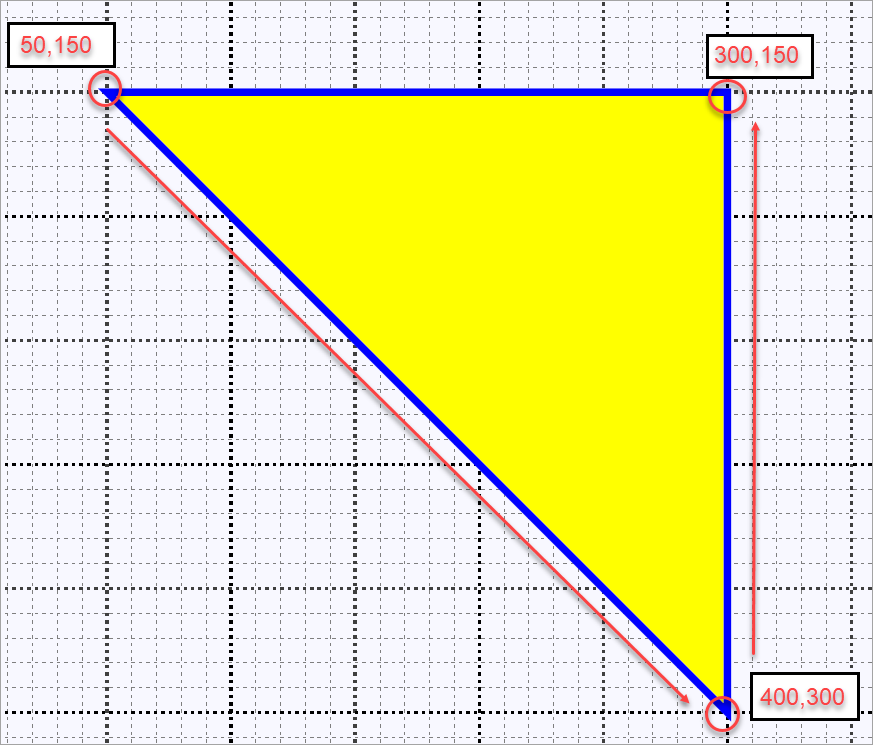
\includegraphics[scale=0.6]{figures/ch5/fig7a}\caption{Adding a triangle to a PDF document.}\label{mar:a-Adding-a-triangle}
\end{figure}
Imagine you have a pen and are drawing
the path. First, you create a new \texttt{Path}\index{Path} instance at 50, 150
and so you place your pen at that point. Next you add a new \texttt{LineSubPath}\index{LineSubPath}
at 300, 400 and so you move your pen from the starting point to the
point at 300, 400. You then add another \texttt{LineSubPath}\index{LineSubPath} at 300,
150, and so you move your pen to that point.
 The original \texttt{Path}\index{Path} instance when you started had set the
close path to true, and so you complete the path by moving your pen
from 300, 150 back to 50,150. The result is a triangle (Figure \ref{mar:a-Adding-a-triangle}).

You then pick up your pen and place it at 50, 250. Then move your
pen to 400, 300, drawing a line. After drawing the line, draw a curve
to 500, 350. Then draw a line from 50, 350 back to 50, 250 (Figure
\ref{mar:a-Creating-a-shape}). 
\begin{figure}
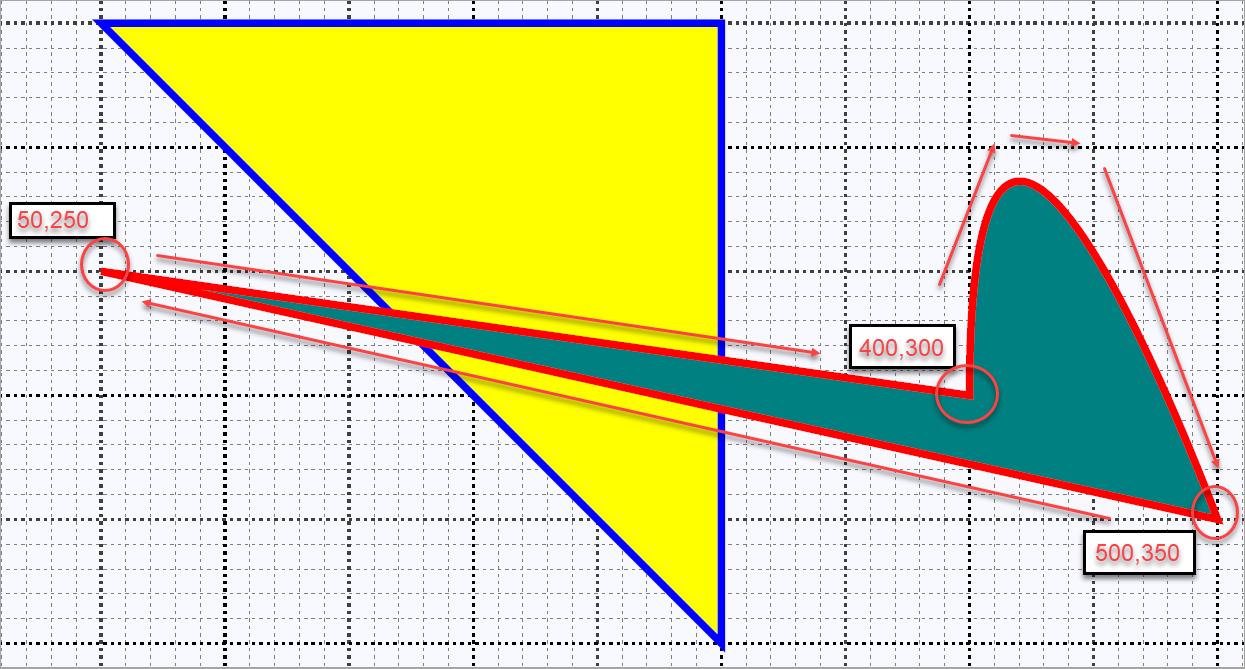
\includegraphics[scale=0.43]{figures/ch5/fig7b}\caption{Creating a shape using a path.}\label{mar:a-Creating-a-shape}
\end{figure}
 Then lift your pen and place it at 50, 450 and draw a line to 60,
475. Then lift your pen and move it to 500, 350 and draw a curve back
to 60, 475. Because the path's constructor initialized the close path to false,
you do not draw a final line to close the shape (Figure \ref{mar:b-Adding-a-path}).
The PDF document consists of three shapes (Figure \ref{fig:Steps-to-adding}).
\begin{figure}
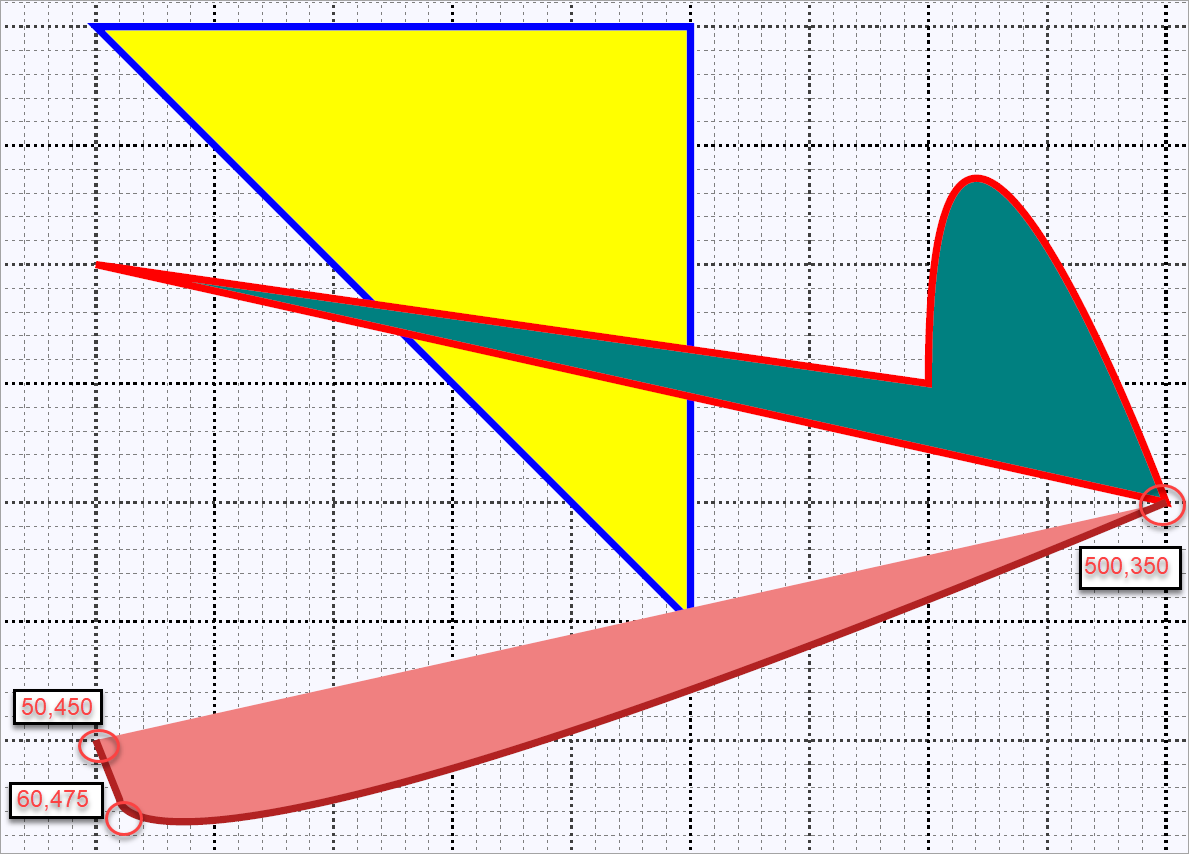
\includegraphics[scale=0.43]{figures/ch5/fig7c}\caption{Adding a path to PDF document.}\label{mar:b-Adding-a-path}
\end{figure}

\begin{figure}

\includegraphics[scale=0.34]{figures/ch5/fig7}\caption{Completed PDF document.}\label{fig:Steps-to-adding}
\end{figure}

\bgroup\inputencoding{latin9}
\begin{lstlisting}[caption={Adding path to a PDF document.},label={lis:Adding-path-to},basicstyle={\small\ttfamily},breaklines=true]
using ceTe.DynamicPDF;
using ceTe.DynamicPDF.PageElements;
using ChapterExamples.Utility;

namespace ChapterExamples.Chapters.ChapterFive
{
    public class PathExample
    {
        public static void Create(string outputPath)
        {
            Document doc = new();
            Page pg = new Page(PageSize.Letter);
            doc.Pages.Add(pg);

            Path pth = new Path(50,50, RgbColor.Blue, RgbColor.Yellow,3, LineStyle.Solid, true);

            pth.SubPaths.Add(new LineSubPath(300, 400));
            pth.SubPaths.Add(new LineSubPath(300, 150));

            Path pth1 = new Path(50, 250, RgbColor.Red, RgbColor.Teal, 3, LineStyle.Solid, false);

            pth1.SubPaths.Add(new LineSubPath(400, 300));
            pth1.SubPaths.Add(new CurveFromSubPath(500, 350, 400, 80));
            pth1.SubPaths.Add(new LineSubPath(50, 250));

            Path pth2 = new Path(50, 450, RgbColor.FireBrick, RgbColor.LightCoral, 3, LineStyle.Solid, false);

            pth2.SubPaths.Add(new LineSubPath(60, 475));
            pth2.SubPaths.Add(new CurveToSubPath(500, 350, 60, 535));
           
            LayoutGrid grid = new();
            grid.ShowTitle = false;

            pg.Elements.Add(grid);
            pg.Elements.Add(pth);
            pg.Elements.Add(pth1);
            pg.Elements.Add(pth2);

            doc.Draw(outputPath);
        }
    }
}
\end{lstlisting}
\leavevmode\egroup

\section{AutoLayout}
\label{section:autolayout-shape}
You can use the \texttt{AutoLayout}\index{AutoLayout} class to add shapes automatically to a \texttt{Document} instance just as you can other page elements (see Chapter \ref{sec:autolayout}). The following example illustrates (Listing \ref{lis:autolayout-shapes}, Figure \ref{mar:autolayout-shape}).
\begin{marginfigure}

\includegraphics[scale=0.55]{figures/ch5/fig8}\caption{Using AutoLayout to create a PDF document.}\label{mar:autolayout-shape}
\end{marginfigure}
\bgroup\inputencoding{latin9}
\begin{lstlisting}[caption={Using AutoLayout to create a PDF document.},label={lis:autolayout-shapes},basicstyle={\small\ttfamily},breaklines=true]
using ceTe.DynamicPDF;
using ceTe.DynamicPDF.PageElements;

namespace ChapterExamples.Chapters.ChapterFive
{
    public class AutoLayoutShapesExample
    {
        public static void Create(string outputPath)
        {
            AutoLayout autoLayout = new AutoLayout(PageSize.Letter, PageOrientation.Portrait, 50);

            Circle myCircle1 = autoLayout.AddCircle(20);
            myCircle1.IgnoreMargins = true;
            myCircle1.BorderStyle = LineStyle.Dots;
            myCircle1.BorderColor = RgbColor.Navy;
            myCircle1.BorderWidth = 5f;
            myCircle1.FillColor = RgbColor.LightGreen;

            Line myLine = autoLayout.AddLine(150, 0, 150, 300);
            myLine.Color = RgbColor.Navy;
            myLine.Width = 4;
            myLine.Cap = LineCap.Butt;

            Rectangle rec2 = autoLayout.AddRectangle(200, 100);
            rec2.BorderColor = RgbColor.Navy;
            rec2.FillColor = RgbColor.Teal;


            Document document = autoLayout.GetDocument();
            document.Draw(outputPath);

        }
    }
}
\end{lstlisting}
\leavevmode\egroup

\section{Summary}

In this chapter, you learned how to add lines, rectangles, circles, and paths to your PDF documents. Since these elements are all page elements, you can place them on either a page or a template. We began by exploring lines using the \texttt{Line} class, then moved on to adding shapes with the \texttt{Rectangle} and \texttt{Circle} classes. Finally, you learned how to use the \texttt{Path} class to create virtually any shape imaginable.

By combining these elements, you can create visually compelling PDF documents. As we’ve seen, shapes not only enhance the aesthetics of a document but also improve clarity and engagement.

In the next chapter, we’ll continue exploring graphical elements by introducing the \texttt{Image} page element. By integrating images with vector graphics, you can create even more dynamic and impressive PDF documents.

\color{white}
\chapter{Images}\label{chap:Images}
\color{black}
\BgThispage
\vspace{8.00em}
\lettrine[lines=2,lhang=0.1]{I}{n} the last chapter, you learned how to add vector-based primitive
shapes to a PDF document. Although using vector-based classes creates
visually appealing documents, you often need to add images. In this
chapter, we examine adding raster graphics to a PDF document. 

Raster graphics (images) are two-dimensional pictures representing
a picture as a rectangular pixel matrix. DynamicPDF Core Suite
for .NET supports nine image types and also supports image transparency.
Supported types include JPEG, PNG, BMP, EMF, WMF, EXIF, JPEG 2000,
GIF, and TIFF. 

Core Suite's \texttt{Image} class handles all types except TIFF. For
the TIFF type, Core Suite provides the \texttt{TiffFile} class for
creating TIFFs. However, as you will see, you access a TIFF file's
underlying images using the Image class. The reason for the different class is, of course, because TIFFs can have multiple images in the same file and must therefore be treated differently than other images.

This chapter examines the various image formats provided and how to
add them to your documents. After learning how to add images to your
PDF documents, you learn how to add a background image to a PDF document
and also an image as a watermark. We then finish the chapter by adding
a 3D image to a PDF document. Upon completing the chapter, you will
understand how to add images to PDF documents and what's possible
using DynamicPDF Core Suite for .NET.

\section{Image}

DynamicPDF Core Suite for .NET provides the \texttt{Image}\index{Image} class
for adding images to a PDF document. You can add images to a document's
\texttt{Page} or \texttt{Template}. As mentioned in the introduction,
supported image types include: JPEG, PNG, BMP, EMF, WMF, EXIF, JPEG
2000, GIF, and TIFF. For every image type but TIFF you use the \texttt{Image}\index{Image}
class to add an image to a page or template. This class has six overloaded
constructors and can take an image from a file, byte array, \texttt{ImageData}\index{ImageData}
class, or \texttt{Stream}. It also has properties for setting its
coordinates, scale, and dimensions. The class also includes methods
for setting its dpi and size.

The \texttt{Image}\index{Image} class has the \texttt{HorizontalDpi}\index{HorizontalDpi}, \texttt{ScaleX}\index{ScaleX},
\texttt{ScaleY}\index{ScaleY}, \texttt{VerticalDpi}\index{VerticalDpi}, and the \texttt{Height}\index{Height} and
\texttt{Width}\index{Width} properties for modifying an image's appearance. It
also has the \texttt{SetBounds(Single)}\index{SetBounds(Single)}, \texttt{SetDpi(Single, Single)}\index{SetDpi(Single, Single)},
and \texttt{SetSize(Single, Single)}\index{SetSize(Single, Single)} methods for modifying an image's
appearance. 

When using an \texttt{Image}\index{Image} instance's properties or methods, it
is important you pay attention to its dimensions and resolution. If
you do not, then often the displayed image appears differently than
expected. So before continuing, lets pause to consider image resolution
and its impact on how an image displays in a PDF document.
\begin{marginfigure}

\includegraphics[scale=0.21]{figures/ch6/egypt12dpi}\caption{Changing the DPI from 72 to 12 for an image.}\label{mar:Changing-the-DPI}
\end{marginfigure}
 

\subsection{Image Resolution}\index{Image Resolution}

In the last chapter, we used vector-based graphics and so they appeared
crisp at any resolution. In contrast, raster images have a specific
resolution, as they are pixel-based. Changing an image's resolution
requires re-sampling the image. However, Core Suite does not re-sample
to change image resolution. When you change an image's resolution,
you must also change its dimensions, as you will see in Listing \ref{lis:Adding-images-to}.
You can change image resolution through the DPI property (dots per
inch), scale, or set the image's height and width. But if changing
an image's height and width manually, be certain to always maintain
the image's aspect ratio. 

The image in Figure \ref{mar:Changing-the-DPI} has an original dimensions
of 840 x 1200 pixels and a 72 dpi resolution. Let's change the resolution
from 72 to 12 dpi.
\begin{marginfigure}
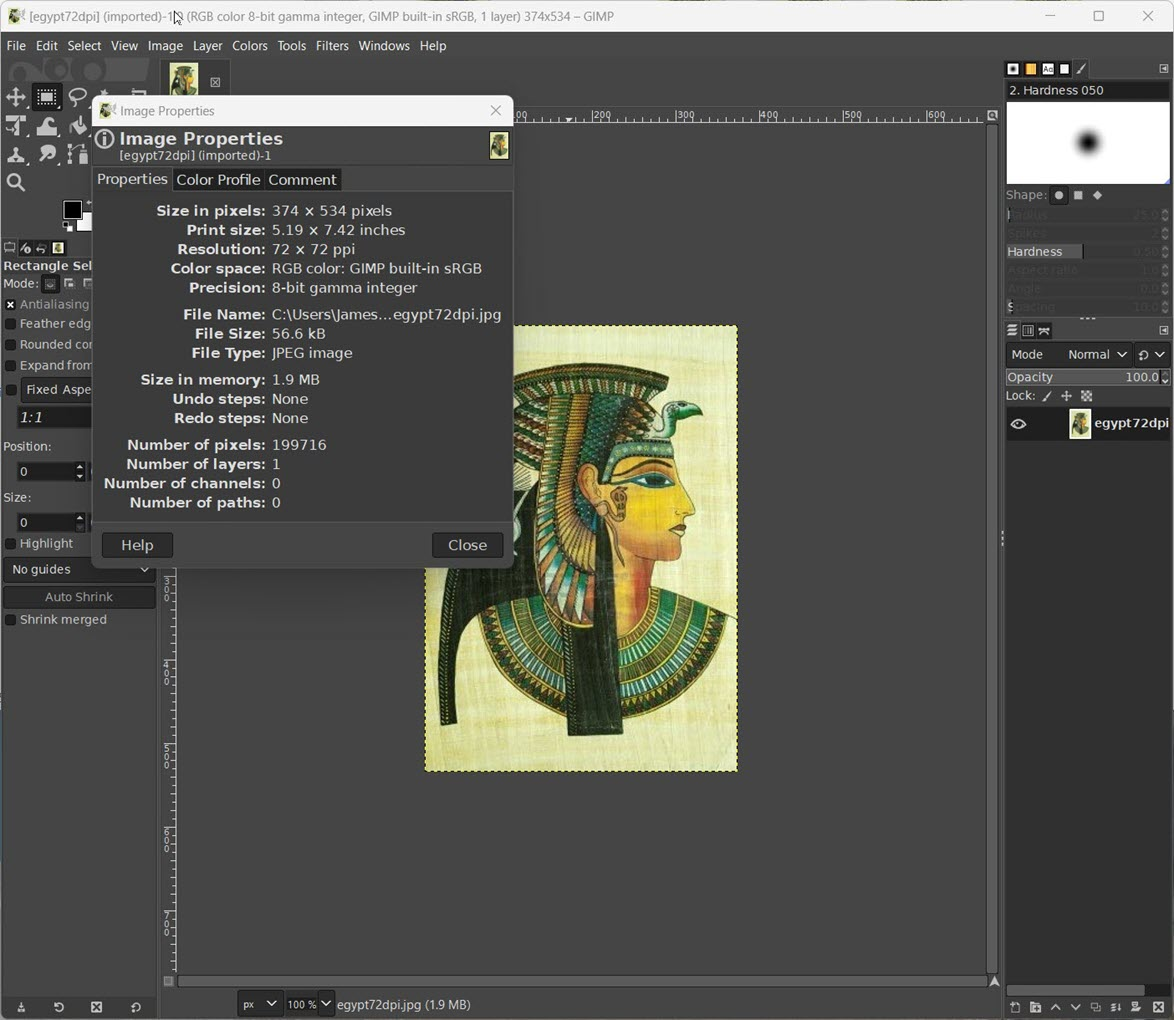
\includegraphics[scale=0.22]{figures/ch6/2024-08-26_15-35-17}\caption{Viewing an image's properties in GIMP.}\label{mar:gimpViewing-an-image's}
\end{marginfigure}
 After changing the resolution, if using software that re-samples,
such as GIMP (Figure \ref{mar:gimpViewing-an-image's}), the re-sampled
image's dimensions become 146 x 206 pixels. Changing the dpi maintained
the images aspect ratio (Figure \ref{mar:Changing-the-DPI}). If we
return to the original image but change the dimensions to 374 x 543,
although the image's size changes, the dpi remains 72. This distinction
is essential, as you can resize without losing resolution, but you
cannot change resolution and then resize the image to larger dimensions
without losing image clarity. Increasing the size of an image after
reducing the dpi results in a loss of resolution.
\begin{figure}

\includegraphics[scale=0.05]{figures/ch6/egypt12dpi-blowup}\caption{Increasing the size of an image after reducing the dpi results in
loss of resolution.}\label{mar:Increasing-the-size}
\end{figure}

After changing an image's dpi you cannot increase its size without
loosing resolution. Notice the difference when you try to change the
image's size in Figure \ref{mar:Changing-the-DPI} to the original
840 x 1200 pixels. Because the image is 12 dpi, when the size is increased
the image looses clarity (Figure \ref{mar:Increasing-the-size}). 

A good rule of thumb is if you simply want to resize a graphic and
not lose resolution, if you have a specific dimension in mind for
an image, then first load the image into an image editing software,
such a GIMP (Figure \ref{mar:gimpViewing-an-image's}), and find the
desired dimensions and resolution. Use those values when creating
your PDF document. Alternatively, if you only want to make an image
smaller with no specific size in mind, then modify the scale in the
constructor or using its properties. 

\subsection{Example}

The example in Listing \ref{lis:Adding-images-to} illustrates adding
the same image, modified three different ways, to a PDF document (Figure
\ref{fig:Modifying-dimensions-of}). First, you add the image and reduce
its scale by 25\% (A). Note that you change both the \texttt{ScaleX}\index{ScaleX}
and \texttt{ScaleY}\index{ScaleY} properties to 25\%. You then change the next image's
dpi to twelve using the \texttt{SetDpi}\index{SetDpi} method. However, you also change
the width and height, carefully maintaining the image's aspect ratio.
Recall that Core Suite does not re-sample an image when changing dpi,
so you also have to reduce the size (B). The third image changes the
image's size manually but maintains its aspect ratio (C). Finally,
the fourth image illustrates that despite violating the image's dimensions,
the \texttt{SetBounds(float maximumWidth, float maximumHeight)} method
scales the image to fit in the given box and maintains the image's
scale (D). Figure \ref{fig:Modifying-dimensions-of} illustrates the
resulting PDF document.
\begin{figure}

\includegraphics[scale=0.20]{figures/ch6/fig8}\caption{Modifying image dimensions.}\label{fig:Modifying-dimensions-of}
\end{figure}

\bgroup\inputencoding{latin9}
\begin{lstlisting}[caption={Adding images to a PDF document.},label={lis:Adding-images-to},basicstyle={\small\ttfamily},breaklines=true]
using ceTe.DynamicPDF;
using ceTe.DynamicPDF.Imaging;
using ceTe.DynamicPDF.PageElements;

namespace ChapterExamples.Chapters.ChapterSix
{
    public class ImageExample
    {
        public static void Create(string resourcePath, string outputPath)
        {
            Document doc = new();
            doc.Pages.Add(new Page(PageSize.Letter));

            Image img1 = new(resourcePath + "/ch2/egypt.jpg",100,100);
            img1.ScaleX = .25f;
            img1.ScaleY = .25f;

            Image img2 = new(resourcePath + "ch2/egypt.jpg", 100, 100);
            img2.SetDpi(12);
            img2.Width = 146;
            img2.Height = 206;

            Image img3 = new(resourcePath + "/ch2/egypt.jpg", 0, 0);
            img3.Width = 374;
            img3.Height = 543;

            Image img4 = new(resourcePath + "/ch2/egypt.jpg", 0, 0);
            img4.SetBounds(200, 200);


            doc.Pages[0].Elements.Add(img1);
            doc.Pages.Add(new Page(PageSize.Letter));
            doc.Pages[1].Elements.Add(img2);
            AddImageData(img2, doc.Pages[1]);

            doc.Pages.Add(new Page(PageSize.Letter));
            doc.Pages[2].Elements.Add(img3);

            doc.Pages.Add(new Page(PageSize.Letter));
            doc.Pages[3].Elements.Add(img4);
            
            doc.Draw(outputPath);
        }
    }
}
\end{lstlisting}
\leavevmode\egroup


\subsection{ImageData}
\begin{marginfigure}

\includegraphics[scale=0.20]{figures/ch6/fig12}\caption{Adding a JPEG using the JpegImageData class.}\label{mar:Adding-a-jpeg}
\end{marginfigure}
You can also create an image using one of the \texttt{ImageData}\index{ImageData} class's
concrete classes: \texttt{GifImageData}\index{GifImageData}, \texttt{Jpeg2000ImageData}\index{Jpeg2000ImageData},
\texttt{JpegImageData}\index{JpegImageData}, \texttt{PngImageData}\index{PngImageData}, and \texttt{TiffImageData}\index{TiffImageData}.

This class provides an image's properties in addition to the underlying
image. Listing \ref{lis:imagedata-jpg-Adding-an-Image} illustrates
using the \texttt{JpegImageData}\index{JpegImageData} class to create an image and add
it to a PDF document.

You first load a jpeg image's data into a \texttt{JpegImageData}\index{JpegImageData} instance.
You then use the \texttt{JpegImageData}\index{JpegImageData} instance to create a new \texttt{Image}\index{Image}
instance and add it to a document page (Figure \ref{mar:Adding-a-jpeg}).\sidenote{Image by By Aaron Ruy Musa , CC BY-SA 4.0. }

\bgroup\inputencoding{latin9}
\begin{lstlisting}[caption={Adding an image using image's data.},label={lis:imagedata-jpg-Adding-an-Image},basicstyle={\small\ttfamily},breaklines=true]
using ceTe.DynamicPDF;
using ceTe.DynamicPDF.Imaging;
using ceTe.DynamicPDF.PageElements;

namespace ChapterExamples.Chapters.ChapterSix
{
    public class JpegDataExample
    {

        //By Aaron Ruy Musa - Own work, CC BY-SA 4.0, https://commons.wikimedia.org/w/index.php?curid=134986047

        public static void Create(string resourcPath, string outputPath)
        {
            Document doc = new();
            doc.Pages.Add(new Page(PageSize.Letter, PageOrientation.Landscape));
            JpegImageData jpgData = new(resourcPath);
            Image img = new Image(jpgData, 0, 0);        
            doc.Pages[0].Elements.Add(img);
            doc.Draw(outputPath);
        }
    }
}
\end{lstlisting}
\leavevmode\egroup

\section{Tiff Images}

Core Suite handles TIFFs differently than the other formats. You add
TIFF images to a PDF using the \texttt{TiffFile}\index{TiffFile} class. This class
has three overloaded constructors and two properties: \texttt{FirstImage}\index{FirstImage}
and \texttt{Image}\index{Image}. Tiffs are unique from other images, as they can
contain multiple images in the same file. 

There are two different ways to handle TIFFs when using Core Suite.
The first, and easiest way, is by creating a new PDF document from
the TIFF. And if a TIFF is multi-page, then each image is a separate
page. The second way to handle a TIFF is by extracting the individual
images from the TIFF and placing the extracted image on a page or
template as a page element. The difference is whether you wish the
entire TIFF to become a new PDF or if you wish the TIFF image(s) to
be extracted and added to an existing PDF. This distinction will become
more obvious in the next sections.

\subsection{Project Setup}

Before illustrating the different ways we can handle TIFFs, let's
first setup the example class. Use the \texttt{TiffExample} class
to consolidate the different ways of handling TIFFs into distinct
methods. As Listing \ref{lis:tif-Example-illustrating-handling} illustrates,
you create four different methods where you demonstrate creating
a new document from a TIFF (Listing \ref{lis:tif-Creating-a-document}).
Then, you demonstrate adding a TIFF's image to a document's page (Listing
\ref{lis:Adding-a-tiff's}). Next, you create a new document from a
multi-page TIFF (Listing \ref{lis:tiff-multi-Creating-a-new}). And
then finally, you extract the images from a multi-page TIFF and add
each image to a separate page (Listing \ref{lis:tif-Adding-images-from}).
You implement each method in the remaining sections, beginning with
creating a PDF directly from a TIFF.

\bgroup\inputencoding{latin9}
\begin{lstlisting}[caption={Handling TIFFs.},label={lis:tif-Example-illustrating-handling},basicstyle={\small\ttfamily},breaklines=true]

using ceTe.DynamicPDF;
using ceTe.DynamicPDF.Imaging;
using ceTe.DynamicPDF.PageElements;

namespace ChapterExamples.Chapters.ChapterSix
{
    public class TiffExample
    {
        public static void Create(string resourcePath, string outputPath)
        {
            CreateNewDoc(resourcePath, outputPath);
            AddTiffToDoc(resourcePath, outputPath);
            MultiPageAddTiffToDoc(resourcePath, outputPath);
            CreateNewDocMultipage(resourcePath, outputPath);
        }
    }
}
\end{lstlisting}
\leavevmode\egroup


\subsection{Create Document}

If you only wish to create a PDF document from a TIFF, then simply
call the \texttt{TiffFile}\index{TiffFile} class's \texttt{GetDocument}\index{GetDocument} method. In
Listing \ref{lis:tif-Creating-a-document} you pass a path to the TIFF
file to the \texttt{TiffFile}\index{TiffFile} class constructor and instantiate a
new instance. You then call the instance's \texttt{GetDocument}\index{GetDocument} method
which returns the entire TIFF image as a PDF document. After outputting
the TIFF to a PDF, you close the TIFF using the \texttt{TiffFile}\index{TiffFile} class's
\texttt{Close}\index{Close} method.\marginnote{Always call the Close method for a TiffFile to prevent
memory leaks.}

\bgroup\inputencoding{latin9}
\begin{lstlisting}[caption={Creating a document from a TIFF.},label={lis:tif-Creating-a-document},basicstyle={\small\ttfamily},breaklines=true]
public static void CreateNewDoc(string resourcePath, string outputPath){
  TiffFile myTiff = new TiffFile(resourcePath + "model.tif");
    Document doc = myTiff.GetDocument();
    doc.Draw(outputPath + "tiff-doc-out.pdf");
  myTiff.Close();
}
\end{lstlisting}
\leavevmode\egroup

Note that when using the \texttt{GetDocument}\index{GetDocument} method, your customization
options are limited. Moreover, you cannot add new pages to the document. You can only get the single image from the TIFF.

\subsection{Add to Document}

The more flexible way to add TIFFs to a document is by accessing the
TIFF file's images. In Listing \ref{lis:Adding-a-tiff's} we create
a new \texttt{TiffFile}\index{TiffFile} instance from a TIFF file. As this TIFF has
only one image, we extract the single image from the \texttt{TiffFile}\index{TiffFile}
instance's \texttt{Images}\index{Images} collection and then create a new \texttt{Image}\index{Image}.
We then add the image as an element to our page and create the PDF
document (Figure \ref{mar:tiff-Adding-an-image}).
\begin{figure}

\includegraphics[scale=0.2]{figures/ch6/fig10}\caption{Adding an image from TIFF to a page.}\label{mar:tiff-Adding-an-image}
\end{figure}

\bgroup\inputencoding{latin9}
\begin{lstlisting}[caption={Adding a TIFF's image to a page.},label={lis:Adding-a-tiff's},basicstyle={\small\ttfamily},breaklines=true]
public static void AddTiffToDoc(string resourcePath, string outPath) {
  Document doc = new();
  doc.Pages.Add(new Page(PageSize.Letter));
     
  TiffFile myTiff = new TiffFile(resourcePath + "model.tif");
  doc.Pages[0].Elements.Add(new Image(myTiff.Images[0], 0, 0, .5f));
  doc.Pages.Add(new Page(PageSize.Letter));
  doc.Draw(outPath + "tiff-added-to-page-out.pdf");
  myTiff.Close();
}
\end{lstlisting}
\leavevmode\egroup


\subsection{Multi-Page TIFFs}

A TIFF file can contain more than one image. Let's return to the \texttt{TiffFile}\index{TiffFile}
class's\texttt{ GetDocument}\index{ GetDocument} method, but consider the created PDF
when a TIFF is a multi-page TIFF. Converting a multi-page TIFF to
a PDF creates a separate page for each image comprising the TIFF.
Listing \ref{lis:tiff-multi-Creating-a-new} illustrates creating
a PDF document from a multi-page TIFF. The code is the same as in
Listing \ref{lis:tif-Creating-a-document}, but the resulting PDF
document has multiple pages (Figure \ref{mar:multipage-tiffCreating-a-new}).
\begin{figure}

\includegraphics[scale=0.2]{figures/ch6/fig11}\caption{Creating a new PDF document from a multi-page TIFF.}\label{mar:multipage-tiffCreating-a-new}
\end{figure}

\bgroup\inputencoding{latin9}
\begin{lstlisting}[caption={Creating a document from multi-page TIFF.},label={lis:tiff-multi-Creating-a-new},basicstyle={\small\ttfamily},breaklines=true]
public static void CreateNewDocMultipage(string resourcePath, string outputPath){
  TiffFile myTiff = new TiffFile(resourcePath + "multipage.tiff");
  Document doc = myTiff.GetDocument();
  doc.Draw(outputPath + "tiff-doc-multi-out.pdf");
  myTiff.Close();
}
\end{lstlisting}
\leavevmode\egroup

Of course, like the previous example where we obtained the single
underlying image (Listing \ref{lis:Adding-a-tiff's}), when there
are multiple images you can extract each using the \texttt{TiffFile}\index{TiffFile}
class's \texttt{Images}\index{Images} collection and create a new \texttt{Image}\index{Image}
instance for each image. Listing \ref{lis:tif-Adding-images-from}
illustrates (Figure \ref{mar:mul-tif-Adding-images-from}).
\begin{figure}

\includegraphics[scale=0.2]{figures/ch6/fig9}\caption{Adding images from a multi-page TIFF to a PDF document.}\label{mar:mul-tif-Adding-images-from}
\end{figure}

\bgroup\inputencoding{latin9}
\begin{lstlisting}[caption={Adding multi-page tiff images to pages.},label={lis:tif-Adding-images-from},basicstyle={\small\ttfamily},breaklines=true]
public static void MultiPageAddTiffToDoc(string resourcePath, string outputPath)
{
  Document doc = new();
  doc.Pages.Add(new Page(PageSize.Letter));
  doc.Pages.Add(new Page(PageSize.Letter));

  TiffFile myTiff = new TiffFile(resourcePath + "multipage.tiff");
  doc.Pages[0].Elements.Add(new Image(myTiff.Images[0], 0, 0, .25f));
  doc.Pages[1].Elements.Add(new Image(myTiff.Images[1], 0, 0, .25f));
  doc.Draw(outputPath + "tiff-multipage-added-to-page-out.pdf");
  myTiff.Close();
}
\end{lstlisting}
\leavevmode\egroup


\section{BackgroundImage}

Now that we know how to add images to a PDF, let's consider background
images. DynamicPDF Core Suite for .NET supports adding background
images to a PDF document through the \texttt{BackgroundImage}\index{BackgroundImage} class.
Listing \ref{lis:Adding-a-background} illustrates adding a background
image to a PDF document.

You first create a new \texttt{BackgroundImage} class instance from an image
file. You then add it to the our page's \texttt{Elements} collection to add
it to the page as a background image.

\bgroup\inputencoding{latin9}
\begin{lstlisting}[caption={Adding a background image.},label={lis:Adding-a-background},basicstyle={\small\ttfamily},breaklines=true]
using ceTe.DynamicPDF;
using ceTe.DynamicPDF.PageElements;
using ChapterExamples.Utility;

namespace ChapterExamples.Chapters.ChapterSix
{
    public class BackgroundImageExample
    {
        public static void Create(string resourcePath, string outputPath)
        {
            Document doc = new();
            doc.Pages.Add(new Page(PageSize.Letter));
            TextArea txt = new(TextGenerator.GenerateTextMultiple(3), 0, 0, 512, 692);
            BackgroundImage img = new(resourcePath);
            doc.Pages[0].Elements.Add(img);
            doc.Pages[0].Elements.Add(txt);
            doc.Draw(outputPath);
        }
    }
}
\end{lstlisting}
\leavevmode\egroup
\begin{figure}

\includegraphics[scale=0.45]{figures/ch6/fig6}\caption{Adding a background image to a PDF document.}\label{fig:Adding-a-background}
\end{figure}

The results of Listing \ref{lis:Adding-a-background} are shown in
Figure \ref{fig:Adding-a-background}. Note that the image is sized
to the page's dimensions.\sidenote{If you wished adding a background image to a page's content within
its margin's bounds, then you would use a \texttt{Template} and add
the image to the \texttt{Template}.}

\section{ImageWatermark}

An \texttt{ImageWatermark}\index{ImageWatermark} is similar to a \texttt{BackgroundImage},
however it automatically applies transparency to the image, thus making
it a watermark. You must add the watermark to each page of your document or use a \texttt{Template}. \marginnote{You must add a watermark to a Template if you wish it to appear on multiple pages.}}Listing \ref{lis:Adding-a-watermark} illustrates (Figure \ref{mar:Adding-a-watermark}).

\bgroup\inputencoding{latin9}
\begin{lstlisting}[caption={Adding a watermark.},label={lis:Adding-a-watermark},basicstyle={\small\ttfamily},breaklines=true]
using ceTe.DynamicPDF;
using ceTe.DynamicPDF.PageElements;
using ChapterExamples.Utility;

namespace ChapterExamples.Chapters.ChapterFive
{
    public class ImageWatermarkExample
    {
        public static void Create(string resourcePath, string outputPath)
        {
            Document doc = new();
            doc.Pages.Add(new Page(PageSize.Letter));
            TextArea txt = new(TextGenerator.GenerateTextMultiple(3), 0, 0, 512, 692);
            ImageWatermark watermark = new(resourcePath);
            doc.Pages[0].Elements.Add(txt);
            doc.Pages[0].Elements.Add(watermark);
            doc.Draw(outputPath);
        }
    }
}
\end{lstlisting}
\leavevmode\egroup

\begin{figure}

\includegraphics[scale=0.25]{figures/ch6/fig4}\caption{Adding a watermark to a PDF document.}\label{mar:Adding-a-watermark}
\end{figure}

\section{Image3d}

The final topic we consider are 3D images. In reality, this topic
deserves an entire chapter, possibly even an entire book, as there
is so much you can do with 3D images. However, here we assume that
if you are creating complex PDF documents designed for users to manipulate
3D objects, then chances are you are using Adobe Acrobat Pro to create
your PDF or some other software dedicated to using 3D modeling to
create PDF documents. Here we only demonstrate that Core Suite includes
this functionality and we provide a basic example illustrating its
use for creating a PDF document with 3D models.

The \texttt{Image3d}\index{Image3d} class adds 3D images of type \texttt{u3d}\index{u3d} and
\texttt{pcx}\index{pcx} to a PDF document.\marginnote{Note that PDF documents only support the .u3d and .pcx 3D image types} Using PDF viewers such as Adobe Acrobat allows users to manipulate
those 3D objects, including changing views and manually moving objects.
Core Suite supports 3D image manipulation by providing the \texttt{View3DProperties}\index{View3DProperties},
\texttt{Image3D}\index{Image3D}, and \texttt{Image3DViewList}\index{Image3DViewList} classes. These classes
allow you to modify how a 3D image is displayed and the image's behavior.
Lets consider a simple example.

\subsection{View3DProperties}

Although you manipulate an image using the \texttt{Image3D}\index{Image3D} class,
how you manipulate the lighting, positioning, background color, and
other aspects of displaying that image rely on the \texttt{View3DProperties}\index{View3DProperties}
class. The \texttt{Image3D}\index{Image3D} class has a \texttt{Image3DViewList}\index{Image3DViewList},
accessed via the image's \texttt{Views}\index{Views} property. The \texttt{Image3DViewList}\index{Image3DViewList}
has a \texttt{Back}, \texttt{Bottom}, \texttt{Default}, \texttt{Front},
\texttt{Isometric}\index{Isometric}, \texttt{Left}, \texttt{Right}, and \texttt{Top}
property that represents the available views. Each view has a \texttt{View3DProperties}\index{View3DProperties}
class, which allows setting the background color, 3D object position,
scaling, field of view, and other properties. To "create" a view,
you set the relevant properties for the relevant view. The view is
then displayed in the PDF reader's list of views when loading the
3D image (Figure \ref{mar:Adobe-Acrobat-displaying}).
\begin{marginfigure}
\raggedright


\includegraphics[scale=0.4]{figures/ch6/fig13}\caption{Adobe Acrobat displaying a list of available views.}\label{mar:Adobe-Acrobat-displaying}

\end{marginfigure}


\subsection{Example}

The following example illustrates adding a 3D image that has three
different views to a PDF document (Listing \ref{lis:image3Adding-a-3D}).
First, we load our 3d model into an \texttt{Image3D} instance using the class's
constructor. We then position the model and how it behaves by defining
its transformation matrix, orbit center, scaling, and other properties.\sidenote{Setting proper transformation matrices and orbit centrality are beyond
this book's scope.} Note that we set different properties for our different views. We
set property values for the \texttt{Default} view, \texttt{Front}
view and \texttt{Back} view. We then add the \texttt{Image3D}\index{Image3D} instance
to our document.

Figure \ref{fig:3d-Results-of-adding} illustrates the resulting PDF
document. The default view and the front view show the object's front,
while the back view shows the object's back. When first loaded into
Acrobat, it shows the view's default view. A user can change the view
by selecting another view from the drop-down. Note in Figure
\ref{fig:3d-Results-of-adding} the view only has two choices: front
and back (Figure \ref{mar:Adobe-Acrobat-displaying}). You can also
manipulate the image using your mouse and you can reset the image.
Of course, there is much more you can do, including some quite complex
scene manipulation and model manipulation; however, that is outside
this book's scope.

\bgroup\inputencoding{latin9}
\begin{lstlisting}[caption={Adding a 3D image.},label={lis:image3Adding-a-3D},basicstyle={\small\ttfamily},breaklines=true]
using ceTe.DynamicPDF;
using ceTe.DynamicPDF.Imaging;
using ceTe.DynamicPDF.PageElements;

namespace ChapterExamples.Chapters.ChapterSix
{
    public class Image3dExample
    {
        public static void Create(string inputPath, string outputPath)
        {
            Document doc = new();
            doc.Pages.Add(new Page(PageSize.Letter));
            
            Image3D image3D = new Image3D(inputPath + "model.u3d", 0, 0, 500, 500);
            float[] front = new float[] {1f,0f,0f,0f,1f,0f,0f,0f,-1f, 0f, 0f,0f};

           View vwDflt = image3D.Views.Default;
           View vwFrnt = image3D.Views.Front;
           View vwBck =  image3D.Views.Back;

            vwDflt.TransformationMatrix = front;
            vwDflt.CenterOfOrbit = 1f;
            vwDflt.OrthographicScaling = .95f;
            vwDflt.Default.BackgroundColor = RgbColor.LightBlue;
            vwDflt.LightingScheme = Lighting3DScheme.Day;

            vwFrnt.BackgroundColor = RgbColor.LightSeaGreen;
            vwFrnt.LightingScheme = Lighting3DScheme.Day;
            vwFrnt.TransformationMatrix = front;
            vwFrnt.CenterOfOrbit = 1f;
            vwFrnt.OrthographicScaling = .95f;

            float[] back = new float[] {1f,0f,0f,0f,1f,0f,0f,0f,1f,0f,0f,0f};

            vwBck.BackgroundColor = RgbColor.LightGreen;
            vwBck.LightingScheme = Lighting3DScheme.Day;
            vwBck.TransformationMatrix = back;
            vwBck.CenterOfOrbit = 1f;
            vwBck.OrthographicScaling = .95f;

            ImageData imgDt = ImageData.GetImage(inputPath + "model.png");
            image3D.PosterImage = imgDt;

            doc.Pages[0].Elements.Add(image3D);
            doc.Draw(outputPath);
        }
    }
}
\end{lstlisting}
\leavevmode\egroup

\begin{figure}[h]

\includegraphics[scale=0.25]{figures/ch6/fig1}\caption{Results of adding and manipulating a 3D object on PDF document.}\label{fig:3d-Results-of-adding}
\end{figure}
\section{AutoLayout}
\label{section:autolayout-image}
You can use the \texttt{AutoLayout}\index{AutoLayout} class to add images automatically to a \texttt{Document} instance just as you can other page elements (see Chapter \ref{sec:autolayout} and \ref{section:autolayout-shape}). The following example illustrates (Listing \ref{lis:autolayout-images}).

\bgroup\inputencoding{latin9}
\begin{lstlisting}[caption={Using AutoLayout to create a PDF document.},label={lis:autolayout-images},basicstyle={\small\ttfamily},breaklines=true]

using ceTe.DynamicPDF;
using ceTe.DynamicPDF.PageElements;

namespace ChapterExamples.Chapters.ChapterSix
{
    public class AutoLayoutImagesExample
    {
        public static void Create(string resourcePath, string outputPath)
        {
            AutoLayout autoLayout = new AutoLayout(PageSize.Letter, PageOrientation.Portrait, 50);

            Image img1 = autoLayout.AddImage(resourcePath + "ch2/egypt.jpg");
            img1.X = 100;
            img1.Y = 100;
            img1.ScaleX = .25f;
            img1.ScaleY = .25f;


            Document document = autoLayout.GetDocument();
            document.Draw(outputPath);

        }
    }
}
\end{lstlisting}
\leavevmode\egroup

\section{Summary}

Adding images to your documents is not just a feature; it's a way
to bring your documents to life. In this chapter, you learned how
to add images and TIFF images to PDF documents. Use the Image class
to add images to a PDF document. Use one of the \texttt{ImageData}
class's child classes to access a particular image type's underlying
data. Use the \texttt{TiffFile} combined with its \texttt{Images}
collection to access a TIFF file's underlying images. 

You also learned how to add background images and watermarks to PDF
documents. Use the \texttt{BackgroundImage} to add background images
and \texttt{ImageWatermark} if you wish the background image to be
a watermark. And finally, you learned how to add 3D images to your
documents using the \texttt{Image3D} class. 

Now that we understand adding images to PDF documents, in the next
chapter, we change our attention to exploring how to group page elements
when creating PDF documents. In that chapter you learn how to anchor
multiple page elements to margins. You also learn how to transform
groups of page elements and apply transparency to those elements as
a unit rather than individually.

\color{white}
\chapter{Grouping}\label{chap:Page-Elements--grouping}
\color{black}
\BgThispage
\vspace{8.00em}
\lettrine[lines=2,lhang=0.1]{T}{his} chapter teaches you how to treat page elements as a single unit.
In the previous chapters, when adding a page element to a page, you
were required to add it to the page's elements collection. When using
one of Core Suite's grouping classes, you can treat page elements
as a single unit and add them to a page all at once. Moreover, you
can transform the rotation, scale, and opacity of page elements added
to a group. 

The classes we examine in this chapter are the \texttt{ContentArea},
\texttt{AreaGroup}, \texttt{AnchorGroup}, \texttt{TransformationGroup},
and \texttt{TransparencyGroup} classes. Each class is similar, allowing
the grouping of page elements as a single unit. However, where and
how they add the elements as a group varies between the classes. Moreover,
the \texttt{TransformationGroup} and \texttt{TransparencyGroup} allow
page elements to be formatted as a single unit. Using the \texttt{TransformationGroup}
class, you can modify the page element's rotation, scale, and location.
Using the \texttt{TranparencyGroup}, you can modify the page element's
opacity and apply additional opacity effects by specifying blending
using effects such as color burn, color dodge, or soft light.

Let's go ahead and consider examples using each group class to illustrate
its capabilities and how you can use them in your applications.

\section{ContentArea}\label{subsec:ContentArea}

Core Suite provides the \texttt{ContentArea} class for adding page
elements to an area within a PDF document. This class allows
adding all page elements at once and treating them as a group. A \texttt{ContentArea}
class's constructor takes \texttt{x}, \texttt{y}, \texttt{height}, and \texttt{width} parameters to place
and size the group. You then add page elements to the \texttt{ContentArea}
instance and the page elements are added to a page as a group. 

Listing \ref{lis:Content-area-added} illustrates adding page elements
to a \texttt{ContentArea}\index{ContentArea}. You first create a new \texttt{ContentArea}
instance and add it to a page. You then call a method we create, \texttt{DrawOutline},
that adds a rectangle of the same dimensions as the \texttt{ContentArea}\index{ContentArea}.
After adding the rectangle you add a label and image to the \texttt{ContentArea}\index{ContentArea}.
Figure \ref{mar:Content-area-added} illustrates the resulting PDF document.
\begin{marginfigure}

\includegraphics[scale=0.45]{figures/ch7/fig6}\caption{Content area added to PDF.}\label{mar:Content-area-added}

\end{marginfigure}

\bgroup\inputencoding{latin9}
\begin{lstlisting}[caption={Content area added to PDF.},label={lis:Content-area-added},basicstyle={\small\ttfamily},breaklines=true]

using ceTe.DynamicPDF;
using ceTe.DynamicPDF.PageElements;

namespace ChapterExamples.Chapters.ChapterSeven
{
    public class ContentAreaExample
    {
        public static void Create(string filePath, string outputPath)
        {
            Document doc = new();
            doc.Pages.Add(new Page(PageSize.Letter));

            ContentArea contentArea = new(200, 200, 200, 200);
            doc.Pages[0].Elements.Add(contentArea);
            DrawOutline(contentArea);

            Label lbl3 = new("A label", 50, 100, 100, 0);
            lbl3.TextColor = RgbColor.Navy;
            contentArea.Add(lbl3);

            Image img = new(filePath, 0, 0, .25f);
            contentArea.Add(img);

            doc.Draw(outputPath);
        }

        public static void DrawOutline(ContentArea contentArea)
        {
            Rectangle rec = new(0, 0, contentArea.Width, contentArea.Height, RgbColor.Navy, RgbColor.LightGrey, 1f, LineStyle.DashLarge);
            contentArea.Add(rec);
        }
    }
}
\end{lstlisting}
\leavevmode\egroup


\section{AreaGroup}\label{subsec:AreaGroup}

An \texttt{AreaGroup}\index{AreaGroup} class is similar to a \texttt{ContentGroup},
but you can only specify its height and width, the x and y coordinates
are  \texttt{(0,0)} and cannot be changed.\sidenote{The coordinates are actually \texttt{(50,50)} if accounting for the
margin.} Listing \ref{lis:Adding-area-group} illustrates adding an \texttt{AreaGroup}
to a PDF document. The code is essentially the same as the \texttt{ContentArea}
code (Listing \ref{lis:Content-area-added}), only the \texttt{AreaGroup}
instance is placed at the \texttt{(0,0)} coordinates (Figure \ref{fig:Anchor-groups-added}).

\bgroup\inputencoding{latin9}
\begin{lstlisting}[caption={Adding area group to a PDF.},label={lis:Adding-area-group},basicstyle={\small\ttfamily},breaklines=true]

using ceTe.DynamicPDF;
using ceTe.DynamicPDF.PageElements;

namespace ChapterExamples.Chapters.ChapterSeven
{
    public class AreaGroupExample
    {
        public static void Create(string filePath, string outputPath)
        {
            Document doc = new();
            doc.Pages.Add(new Page(PageSize.Letter));

            AreaGroup group = new(400, 400);

            doc.Pages[0].Elements.Add(group);

            DrawOutline(group);

            Label lbl3 = new("A label", 50, 100, 100, 0);
            lbl3.TextColor = RgbColor.Navy;
            group.Add(lbl3);

            Image img = new(filePath, 0, 0, .25f);
            group.Add(img);

            doc.Draw(outputPath);
        }

        public static void DrawOutline(AreaGroup areaGroup)
        {
            Rectangle rec = new(0, 0, areaGroup.Width, areaGroup.Height, RgbColor.Navy, RgbColor.LightGrey, 1f, LineStyle.DashLarge);
            areaGroup.Add(rec);
        }
    }
}
\end{lstlisting}
\leavevmode\egroup

\begin{figure}

\includegraphics[scale=0.40]{figures/ch7/fig5}\caption{Area group added to a PDF.}\label{fig:Area-group-added}
\end{figure}


\section{AnchorGroup}\label{subsec:AnchorGroup}

The \texttt{AnchorGroup}\index{AnchorGroup} class anchors a grouping of page elements
to a page's margins or edges. An \texttt{AnchorGroup}\index{AnchorGroup} class's constructor
has height, width, horizontal alignment and vertical alignment parameters
for laying-out the group. The \texttt{Align} enumeration provides
the following values: \texttt{Center}, \texttt{Left}, and \texttt{Right}.
The \texttt{VAlign} enumeration's values are: \texttt{Bottom}, \texttt{Center},
and \texttt{Top}. The class also has an \texttt{AnchorTo}\index{AnchorTo} property
which takes an \texttt{AnchorTo}\index{AnchorTo} enumeration which can be \texttt{Edges}
or \texttt{Margins}.

In Listing \ref{lis:Adding-anchor-groups} you add three anchor groups
to a PDF document. You first create a new \texttt{AnchorGroup}\index{AnchorGroup} instance
and specify its \texttt{x} and \texttt{y} coordinates and its horizontal and vertical
alignment. You then specify the grouping is anchored to the page's
margins and then add some page elements to the anchor group. 

After creating the first anchor group, you create a second \texttt{AnchorGroup}\index{AnchorGroup}
instance, but you change its horizontal and vertical alignment to be
the page's bottom right. Then, for the third \texttt{AnchorGroup}\index{AnchorGroup}
instance, rather than anchoring it to the page's margins, you anchor
it to the page's edges. Figure \ref{fig:Anchor-groups-added} illustrates
the resulting PDF document.
\begin{figure}

\includegraphics[scale=0.45]{figures/ch7/fig4}\caption{Anchor groups added to PDF.}\label{fig:Anchor-groups-added}
\end{figure}

\bgroup\inputencoding{latin9}
\begin{lstlisting}[caption={Adding anchor groups to PDF.},label={lis:Adding-anchor-groups},basicstyle={\small\ttfamily},breaklines=true]

using ceTe.DynamicPDF;
using ceTe.DynamicPDF.PageElements;

namespace ChapterExamples.Chapters.ChapterSeven
{
    public class AnchorGroupExample
    {

        public static void Create(string filePath, string outputPath)
        {
            Document doc = new();
            doc.Pages.Add(new Page(PageSize.Letter));
            
            AnchorGroup aGrp = new(200, 200, Align.Left, VAlign.Top);
            aGrp.AnchorTo = AnchorTo.Margins;
 
            AnchorGroupExample.drawOutline(aGrp);

            Circle circle = new(50, 50, 5, RgbColor.FireBrick, RgbColor.Tan, 2, LineStyle.Dash);
            aGrp.Add(circle);

            Label lbl = new("Align Left", 50, 75, 100,0);
            lbl.TextColor = RgbColor.Navy;
            aGrp.Add(lbl);
                      
            doc.Pages[0].Elements.Add(aGrp);
                        
            AnchorGroup aGrp2 = new(150, 200, Align.Right, VAlign.Bottom);
            aGrp2.AnchorTo = AnchorTo.Margins;

            AnchorGroupExample.drawOutline(aGrp2);

            Label lbl2 = new("Align Right", 30, 60, 100, 0);
            lbl2.TextColor = RgbColor.Navy;
            aGrp2.Add(lbl2);

            Image img = new(filePath, 0, 0, .25f);
            aGrp2.Add(img);

            doc.Pages[0].Elements.Add(aGrp2);


            AnchorGroup aGrp3 = new(200, 90, Align.Left, VAlign.Center);
            aGrp3.AnchorTo = AnchorTo.Edges;
            AnchorGroupExample.drawOutline(aGrp3);

            Label lbl3 = new("Align Left", 5, 5, 100, 0);
            lbl3.TextColor = RgbColor.Navy;
            aGrp3.Add(lbl3);

            doc.Pages[0].Elements.Add(aGrp3);

            LayoutGrid layGrd = new();
            layGrd.ShowTitle = false;
            doc.Pages[0].Elements.Add(layGrd);

            doc.Draw(outputPath);
        }

        public static void drawOutline(AnchorGroup anchorGroup)
        {
            Rectangle rec = new(0, 0, anchorGroup.Width, anchorGroup.Height, RgbColor.Navy, RgbColor.LightGrey, 1f, LineStyle.DashLarge);
            anchorGroup.Add(rec);
        }
    }
}
\end{lstlisting}
\leavevmode\egroup


\section{TransformationGroup}\label{subsec:TransformationGroup}

Core Suite provides the \texttt{TransformationGroup}\index{TransformationGroup} class to allow
transforming groups of page elements as a single unit. The \texttt{TransformationGroup}\index{TransformationGroup}
class is used to shift, rotate and scale other page elements. Any
page element placed in a transformation group will shift, rotate or
scale with that transformation group.

A \texttt{TransformationGroup}\index{TransformationGroup} class's has two constructors one that
takes an x, y, height, and width parameter for specifying the group's
layout and another that adds an additional angle parameter. The class
has an \texttt{Angle} property for specifying rotation and a \texttt{ScaleX}
and \texttt{ScaleY} property for specifying scaling. All page elements
added to the transformation group are transformed in unison as Listing
\ref{lis:Applying-a-TransformationGroup} illustrates.

In Listing \ref{lis:Applying-a-TransformationGroup} you create a \texttt{TransformationGroup}\index{TransformationGroup}
instance and specify an angle and scale factor. You then add an image
and some text to the instance. You also create a circle, but add it
to the page rather than the grouping. Figure \ref{mar:PDF-document-with}
illustrates the resulting PDF document.
\begin{marginfigure}
\raggedright

\includegraphics[scale=0.25]{figures/ch7/fig3}\caption{PDF document with a TransformationGroup applied.}\label{mar:PDF-document-with}
\end{marginfigure}

\bgroup\inputencoding{latin9}
\begin{lstlisting}[caption={Applying a TransformationGroup.},label={lis:Applying-a-TransformationGroup},basicstyle={\small\ttfamily},breaklines=true]

using ceTe.DynamicPDF;
using ceTe.DynamicPDF.PageElements;
using ChapterExamples.Utility;

namespace ChapterExamples.Chapters.ChapterSeven
{
    public class TransformationGroupExample
    {
        public static void Create(string filePath, string outputPath)
        {
            Document doc = new();
            doc.Pages.Add(new Page(PageSize.Letter));

            TransformationGroup objTgroup = new(300, 300, 100, 200);
            objTgroup.Angle = 90f;
            objTgroup.ScaleX = .75f;
            objTgroup.ScaleY = .75f;

            Image img = new(filePath, 0, 0);
            objTgroup.Add(img);

            string txt = TextGenerator.GenerateTextMultiple(1);
            TextArea txtA = new(txt, 0, 100, 512, 692);
            objTgroup.Add(txtA);

            Circle cir = new(0, 50, 25);
            cir.FillColor = RgbColor.Navy;
            doc.Pages[0].Elements.Add(cir);

            doc.Pages[0].Elements.Add(objTgroup);
            doc.Draw(outputPath);
        }
    }
}
\end{lstlisting}
\leavevmode\egroup


\section{TransparencyGroup}\label{subsec:TransparencyGroup}

Core Suite provides the \texttt{TransparencyGroup}\index{TransparencyGroup} class for applying
transparency to groups of elements at once. The class has two constructors,
one that specifies transparency and another that also specifies the
blend mode. The \texttt{alpha}\index{alpha} parameter species the transparency
to use as a percentage of transparency. The \texttt{blendMode} parameter
and specifies the blending to be applied. Values for \texttt{BlendMode}
are: \texttt{ColorBurn}, \texttt{ColorDodge}, \texttt{Darken}, \texttt{Difference},
\texttt{Exclusion}, \texttt{HardLight}, \texttt{Lighten}, \texttt{Multiply},
\texttt{Normal}, \texttt{Overlay}, \texttt{Screen} and \texttt{SoftLight}.

\bgroup\inputencoding{latin9}
\begin{lstlisting}[caption={Applying transparency to several page elements.},label={lis:Applying-transparency-to},basicstyle={\small\ttfamily},breaklines=true]

using ceTe.DynamicPDF;
using ceTe.DynamicPDF.PageElements;
using ChapterExamples.Utility;

namespace ChapterExamples.Chapters.ChapterSeven
{
    public class TransparencyGroupExample
    {
        public static void Create(string filePath, string outputPath)
        {
            Document doc = new();
            doc.Pages.Add(new Page(PageSize.Letter));
           
            TransparencyGroup objTgroup = new(.25f);

            Image img = new(filePath, 0, 0);
            objTgroup.Add(img);

            string txt = TextGenerator.GenerateTextMultiple(2);
            TextArea txtA = new(txt, 0, 100, 512, 692);
            objTgroup.Add(txtA);

            Circle cir = new(0,50, 25);
            cir.FillColor = RgbColor.Navy;
            doc.Pages[0].Elements.Add(cir);

            doc.Pages[0].Elements.Add(objTgroup);
            doc.Draw(outputPath);
        }

    }
}
\end{lstlisting}
\leavevmode\egroup

\begin{figure}


\includegraphics[scale=0.40]{figures/ch7/fig2}\caption{PDF document with transparency applied to several page elements.}\label{fig:PDF-document-with}

\end{figure}


\section{Summary}

In this chapter, you learned how to group and transform page elements
as a cohesive unit. The \texttt{ContentArea}, \texttt{AreaGroup},
and \texttt{AnchorGroup} classes are essential tools for grouping
multiple page elements and adding them to a page as a single entity.
The \texttt{TransformationGroup}  allows
you to combine page elements into a group and manipulate them collectively,
enabling operations such as rotation, scaling, and shifting as one
unit. Additionally, the \texttt{TransparencyGroup} class allows
you to group page elements and adjust their opacity and blending effects
seamlessly. As you learned, all these classes allow easier PDF document
creation, as you can treat page elements as a single unit rather than
individually. 

\color{white}
\chapter{Fonts and Colors}\label{chap:fonts-colors}
\color{black}
\BgThispage
\vspace{8.00em}
\lettrine[lines=2,lhang=0.1]{I}{n} this chapter we discuss fonts and colors. Although we have addressed
both topics throughout this book, here we explicitly discuss both
and how to use fonts and colors in Core Suite to create more engaging PDF documents.
We start this chapter by discussing fonts. Although Adobe has fourteen
core fonts, you can embed numerous other kinds of fonts into your
PDF documents when using Core Suite. After discussing fonts, we discuss
using colors to create more vibrant PDF documents.\marginnote{This chapter does not fully address professional typesetting and color.}

You first learn the different fonts you can apply to your PDF documents.
We examine the Adobe core fonts, Google fonts, Opentype fonts, and
briefly consider TrueType fonts and CJK fonts. We also discuss Core
Suite's features related to type-setting, such as kerning and tracking.

After learning about Core Suite's font support, we then turn our attention
to Core Suite's support for color. Core Suite supports CMYK, RGB,
Web, and Grayscale colors. It also supports Gradient, Auto Gradient,
and Spot Color. In this chapter we examine each of these types of
colors.

\section{Fonts}\label{sec:Fonts}
DynamicPDF Core Suite for .NET supports numerous diferent fonts, including the Adobe's fourteen core fonts, Google fonts, OpenType fonts, TrueType Collections, Web, and Type fonts, and CJK fonts.  
\subsection{Core Fonts}

The standard fourteen PDF core fonts that can be referenced by name
in a PDF document are:
\begin{itemize}
\item Courier, Courier Bold, Courier Oblique, Courier Bold-Oblique,
\item Helvetica, Helvetica Bold, Helvetica Oblique, Helvetica Bold-Oblique,
\item Times Roman, Times Bold, Time Italic, Times Bold-Italic,
\item Symbol, and
\item Zapf Dingbats.
\end{itemize}
Core Suite provides each of the core fonts as a static property of
the \texttt{Font}\index{Font} class (Table \ref{tab:Core-14-fonts}).
\begin{table}[h]
\begin{tabular}{ll}
\toprule 
{\footnotesize Font Class} & {\footnotesize Font Name}\tabularnewline
\midrule
{\footnotesize\texttt{Font.Courier}} & {\footnotesize Courier}\tabularnewline
{\footnotesize\texttt{Font.CourierBold}} & {\footnotesize Courier Bold}\tabularnewline
{\footnotesize\texttt{Font.CourierOblique}} & {\footnotesize Courier Oblique}\tabularnewline
{\footnotesize\texttt{Font.CourierBoldOblique}} & {\footnotesize Courier Bold Oblique}\tabularnewline
{\footnotesize\texttt{Font.Helvetica}} & {\footnotesize Helvetica (Arial)}\tabularnewline
{\footnotesize\texttt{Font.HelveticaBold}} & {\footnotesize Helvetica (Arial) Bold}\tabularnewline
{\footnotesize\texttt{Font.HelveticaOblique}} & {\footnotesize Helvetica (Arial) Oblique}\tabularnewline
{\footnotesize\texttt{Font.HelveticaBoldOblique}} & {\footnotesize Helvetica (Arial) Bold Oblique}\tabularnewline
{\footnotesize\texttt{Font.Times}} & {\footnotesize Times (Times New Roman)}\tabularnewline
{\footnotesize\texttt{Font.TimesBold}} & {\footnotesize Times (Times New Roman) Bold}\tabularnewline
{\footnotesize\texttt{Font.TimesItalic}} & {\footnotesize Times (Times New Roman) Italic}\tabularnewline
{\footnotesize\texttt{Font.TimesBoldItalic}} & {\footnotesize Times (Times New Roman) Bold Italic}\tabularnewline
{\footnotesize\texttt{Font.Symbol}} & {\footnotesize Symbol}\tabularnewline
{\footnotesize\texttt{Font.ZapfDingbats}} & {\footnotesize Zapf Dingbats}\tabularnewline
\bottomrule
\end{tabular}\caption{Core 14 fonts available to all PDF readers.}\label{tab:Core-14-fonts}
\end{table}
\medskip
Using the \texttt{Font}\index{Font} class with one of the fourteen core fonts
is straightforward; simply refer to the desired font in the \texttt{Font}\index{Font}
class and then set its size (Listing \ref{lis:PDF-document-using}).\marginnote{PDF/UA and PDF/A compliant PDF documents must embed any font used,
even if a core font (Chapter \ref{chap:Accessibility} and Chapter
\ref{chap:Archiving-and-PDF/A}).}

Listing \ref{lis:PDF-document-using} illustrates using the Courier
Bold, Times Roman, and Helvetica Bold-Oblique fonts in a PDF Document
(Figure \ref{fig:PDF-document-using}).

\bgroup\inputencoding{latin9}
\begin{lstlisting}[caption={PDF document using Core Fonts.},label={lis:PDF-document-using},basicstyle={\small\ttfamily},breaklines=true]

using ceTe.DynamicPDF;
using ceTe.DynamicPDF.PageElements;
using ChapterExamples.Utility;

namespace ChapterExamples.Chapters.ChapterEight
{
    public class CoreFontsExample
    {
        public static void Create(string outputPath)
        {
            Document doc = new();
            doc.Pages.Add(new Page(PageSize.Letter));

            float pgWdth = doc.Pages[0].Dimensions.Width - doc.Pages[0].Dimensions.LeftMargin * 2;
            float pgHeight = doc.Pages[0].Dimensions.Height - doc.Pages[0].Dimensions.TopMargin * 2;

            Label lbl = new Label("Chapter One", 10, 10, 150, 50, Font.CourierBold, 22);

            string txt1 = Utility.TextGenerator.GenerateTextMultiple(1);
            TextArea txt = new(txt1, 0, doc.Pages[0].Dimensions.TopMargin, pgWdth, pgHeight, Font.TimesRoman, 14);

            Label lbl2 = new Label("Next Section", 10, pgHeight-150, 150, 50);
            lbl2.Font = Font.HelveticaBoldOblique;
            lbl2.FontSize = 18;

            doc.Pages[0].Elements.Add(lbl);
            doc.Pages[0].Elements.Add(txt);
            doc.Pages[0].Elements.Add(lbl2);

            AddGridLines.AddBackgroundColor(doc);
            doc.Draw(outputPath + "core-fonts.pdf");
        }
    }
}
\end{lstlisting}
\leavevmode\egroup

\begin{figure}

\includegraphics[scale=0.4]{figures/ch8/fig1}\caption{PDF document using Core Fonts.}\label{fig:PDF-document-using}

\end{figure}


\subsection{Google Fonts}

Core Suite also supports any Google Font. Google Fonts provides free
and open source font families that applications can use without a
licensing.\cite{Google123} Access Google Fonts through Google's interactive
web application where you can browse available fonts (www.fonts.google.com).
There you can find the name of the font you wish to use in Core Suite.

Core Suite's \texttt{GoogleFont}\index{GoogleFont} class encapsulates
Google Fonts. This class has numerous properties, the most important
being the \texttt{Name}\index{Name}. This property is the font's
name and you use it to create a new \texttt{GoogleFont}\index{GoogleFont}
instance using the \texttt{Font}\index{Font} class's static \texttt{Google}\index{Google}
method. The \texttt{Google} method has two overloads. The first allows specifying
if the font is bold and specifying if the font is italic. The second
allows specifying the font's weight and if specifying if the font
is italic.

\bgroup\inputencoding{latin9}
\begin{lstlisting}[basicstyle={\small\ttfamily},breaklines=true]
public static GoogleFont Google(string fontName, [bool bold = False], [bool italic = False])
public static GoogleFont Google(string fontName, [int weight = 400], [bool italic = False])
\end{lstlisting}
\leavevmode\egroup

Listing \ref{lis:google-PDF-document-using-1} illustrates creating
a PDF document using three different fonts. You create instances of
the Modak, Caveat, and Roboto fonts. In the first instance you specify
that it will create a \texttt{GoogleFont}\index{GoogleFont} instance of the Modak font
and accepts the default values of false for the bold and italic parameters.
In the second instance you use the Caveat font and set the bold parameter
to true and the italic parameter to false. In the final instance you
uses the Roboto font and set the weight to 100 and italic to true.
Figure \ref{fig:google-PDF-document-using-1} illustrates the produced
PDF document.
\begin{figure}

\includegraphics[scale=0.39]{figures/ch8/fig3}\caption{PDF document using Google fonts.}\label{fig:google-PDF-document-using-1}
\end{figure}

\bgroup\inputencoding{latin9}
\begin{lstlisting}[caption={PDF document using Google fonts.},label={lis:google-PDF-document-using-1},basicstyle={\small\ttfamily},breaklines=true]

using ceTe.DynamicPDF;
using ceTe.DynamicPDF.PageElements;
using ceTe.DynamicPDF.Text;
using ChapterExamples.Utility;

namespace ChapterExamples.Chapters.ChapterEight
{
    public class GoogleFontsExample
    {
        public static void Create(string outputPath)
        {
            Document doc = new();
            doc.Pages.Add(new Page(PageSize.Letter));

           float pgWdth = doc.Pages[0].Dimensions.Width - doc.Pages[0].Dimensions.LeftMargin * 2;
            float pgHeight = doc.Pages[0].Dimensions.Height - doc.Pages[0].Dimensions.TopMargin * 2;

            GoogleFont googleFont = Font.Google("Modak");
            Label lbl = new Label("Chapter One", 10, 10, 150, 50, googleFont, 22);

            string txt1 = Utility.TextGenerator.GenerateTextMultiple(1);
            TextArea txt = new(txt1, 0, doc.Pages[0].Dimensions.TopMargin, pgWdth, pgHeight, Font.Google("Caveat", false, false), 14);

            Label lbl2 = new Label("Next Section", 10, pgHeight - 150, 150, 50);
            lbl2.Font = Font.Google("Roboto", 100, true);
            lbl2.FontSize = 18;

            doc.Pages[0].Elements.Add(lbl);
            doc.Pages[0].Elements.Add(txt);
            doc.Pages[0].Elements.Add(lbl2);

            AddGridLines.AddBackgroundColor(doc);
            doc.Draw(outputPath + "google-fonts.pdf");
        }
    }
}
\end{lstlisting}
\leavevmode\egroup

You must be careful when using Google Fonts to ensure the font supports
bold and/or italics. For example, had you set Italic to true you would
receive an error (Figure \ref{mar:Incorrect-Google-Font}).
\begin{figure}

\includegraphics[scale=0.43]{figures/ch8/fig2}\caption{Incorrect Google Font setting.}\label{mar:Incorrect-Google-Font}

\end{figure}


\subsection{OpenType Fonts}

OpenType fonts are scalable computer font derived from TrueType and
is a registered trademark of Microsoft Corporation. Core Suite creates
instances of OpenType fonts through the \texttt{OpenTypeFont}\index{OpenTypeFont} class
where in the constructor it specifies the path to the font file.

Listing \ref{lis:opentype-PDF-document-using-1} illustrates creating
an \texttt{OpenTypeFont}\index{OpenTypeFont} instance and passing the \texttt{cnr.otf}\index{cnr.otf}
font to its constructor. It then uses the \texttt{OpenTypeFont}\index{OpenTypeFont} object
instance with a \texttt{Label} and a \texttt{TextArea}. Figure \ref{fig:opentype-PDF-document-using-1}
illustrates the resulting PDF document.
\begin{figure}


\includegraphics[scale=0.5]{figures/ch8/fig4}\caption{PDF document using OpenType fonts.}\label{fig:opentype-PDF-document-using-1}

\end{figure}

\bgroup\inputencoding{latin9}
\begin{lstlisting}[caption={PDF document using OpenType Font.},label={lis:opentype-PDF-document-using-1},basicstyle={\small\ttfamily},breaklines=true]
public static void OpenTypeExample(string resourcePath, string outputPath)
{
    Document doc = new();
    doc.Pages.Add(new Page(PageSize.Letter));

    float pgWdth = doc.Pages[0].Dimensions.Width - doc.Pages[0].Dimensions.LeftMargin * 2;
    float pgHeight = doc.Pages[0].Dimensions.Height - doc.Pages[0].Dimensions.TopMargin * 2;

    OpenTypeFont openType = new OpenTypeFont(resourcePath + "cnr.otf");

    Label lbl = new Label("Chapter One", 10, 10, 150, 50, openType, 22);

    string txt1 = Utility.TextGenerator.GenerateTextMultiple(1);
    TextArea txt = new(txt1, 0, doc.Pages[0].Dimensions.TopMargin, pgWdth, pgHeight, openType, 14);

    doc.Pages[0].Elements.Add(lbl);
    doc.Pages[0].Elements.Add(txt);

    AddGridLines.AddBackgroundColor(doc);
    doc.Draw(outputPath + "opentype-fonts.pdf");
}
\end{lstlisting}
\leavevmode\egroup


\subsection{TrueType Collections, Web Fonts, Type1 Fonts}

DynamicPDF Core Suite for .NET also supports these font types
through the \texttt{OpentTypeFontCollection}\index{OpentTypeFontCollection}, \texttt{WebOpenFont}\index{WebOpenFont},
and \texttt{Type1Font}\index{Type1Font} classes. Web fonts are used in web pages on
the web. Core Suite supports only WOFF 1.0. A TrueType Collection
(TTC) is a collection of TrueType fonts combined into a single file.
Using these font classes are the same as other fonts, and so are not
discussed here.

\subsection{CJK Fonts}\index{CJK Fonts}

PDF readers with the Adobe Asian Font Pack installed supports seven
CJK fonts and does not require embedding in a PDF document. Core Suite
supports the these fonts through the following \texttt{Font} class
through the following static properties.
\begin{itemize}
\item Japanese
\begin{itemize}
\item \texttt{Font.HeiseiKakuGothicW5}\index{Font.HeiseiKakuGothicW5}
\item \texttt{Font.HeiseiMinchoW3}\index{Font.HeiseiMinchoW3}
\end{itemize}
\item Korean
\begin{itemize}
\item \texttt{Font.HanyangSystemsGothicMedium}\index{Font.HanyangSystemsGothicMedium}
\item \texttt{Font.HanyangSystemsShinMyeongJoMedium}\index{Font.HanyangSystemsShinMyeongJoMedium}
\end{itemize}
\item Simplified Chinese
\begin{itemize}
\item \texttt{Font.SinoTypeSongLight}\index{Font.SinoTypeSongLight}
\end{itemize}
\item Traditional Chinese
\begin{itemize}
\item \texttt{Font.MonotypeHeiMedium}\index{Font.MonotypeHeiMedium}
\item \texttt{Font.MonotypeSungLight}\index{Font.MonotypeSungLight}
\end{itemize}
\end{itemize}

\subsection{Embedding Fonts}

Fonts that are not present in a user's PDF reader software or on their
system opening a PDF document must have the fonts embedded in the
PDF document or an error occurs. Moreover, as you see in the chapters
on accessibility and archiving (Chapter \ref{chap:Accessibility}
and Chapter \ref{chap:Archiving-and-PDF/A}), you must embed all fonts
in order for your PDF document to meet accessibility and archiving
standards.

Embedding a font is straightforward, as Listing \ref{lis:Embedding-a-font.}
illustrates. After creating the font instance, simply specify \texttt{Embed}
as \texttt{true}. 

\bgroup\inputencoding{latin9}
\begin{lstlisting}[caption={Embedding a font.},label={lis:Embedding-a-font.},basicstyle={\small\ttfamily},breaklines=true]
string text = "PDF/A (Archiving) requires you embedd fonts.";
OpenTypeFont openTypeFont = new OpenTypeFont("times.ttf");
opentypeFont.Embed = true;
Label label = new Label(text, 0, 0, 504, 100, openTypeFont, 18, TextAlign.Center, RgbColor.BlueViolet);
\end{lstlisting}
\leavevmode\egroup


\subsection{Text Encoding}

When using a non-symbolic Core Font with Core Suite, Latin 1 encoding
is the default. Specify alternate encodings as needed to allow access
to characters specific to other encodings. Core Suite provides the
\texttt{Encoder}\index{Encoder} class which has the following static properties:
\texttt{Encoder.CentralEurope}\index{Encoder.CentralEurope}, \texttt{Encoder.Latin1}\index{Encoder.Latin1},
\texttt{Encoder.Turkish}\index{Encoder.Turkish}, \texttt{Encoder.Baltic}\index{Encoder.Baltic},
\texttt{Encoder.Latin2}\index{Encoder.Latin2}, and  \texttt{ Encoder.Latin9}\index{ Encoder.Latin9}.
Although we do not discuss encoding in depth, the following example
illustrates (Listing \ref{lis:Encoding-a-PDF}).

Listing \ref{lis:Encoding-a-PDF} illustrates encoding a string in
Czech where:
\noindent\begin{flushleft}
\texttt{txtString = \textquotedbl čárka nad písmenem, silný
přízvuk''.} 
\par\end{flushleft}

First, we create a new \texttt{Font} instance and specify
the encoding as central European. Thenyou create a new \texttt{TextArea}
with a simple string and in the \texttt{TextArea} constructor
you specify \texttt{Encoder.CentralEurope}\index{Encoder.CentralEurope}. You then create
three labels. The first is the Czech string without specifying the
label's font encoding. The second label is the English translation
of the Czech string. The third label is also the Czech string, but
with the proper encoding applied. Figure \ref{mar:Encoding-a-PDF}
illustrates the results. 

\bgroup\inputencoding{latin9}
\begin{lstlisting}[caption={Encoding a PDF document.},label={lis:Encoding-a-PDF},basicstyle={\small\ttfamily},breaklines=true]
public static void EncodingExample(string resourcePath, string outputPath)
 {
     Document doc = new();
     doc.Pages.Add(new Page(PageSize.Letter));

     float pgWdth = doc.Pages[0].Dimensions.Width - doc.Pages[0].Dimensions.LeftMargin * 2;
     float pgHeight = doc.Pages[0].Dimensions.Height - doc.Pages[0].Dimensions.TopMargin * 2;

     Font centralEuropeHelveticaFont = new Helvetica(Encoder.CentralEurope);
     TextArea txt = new TextArea(txtString, 0, 0, 200, 12, centralEuropeHelveticaFont, 12);

     Label lbl = new(txtString, 0, 100, 300, 0, Font.Helvetica, 12);
     Label lbl2 = new("comma above the letter, strong accent", 0, 125, 300, 0, Font.Helvetica, 12);
     Label lbl3 = new(txtString, 0, 150, 300, 0, centralEuropeHelveticaFont, 12);

     doc.Pages[0].Elements.Add(txt);
     doc.Pages[0].Elements.Add(lbl);
     doc.Pages[0].Elements.Add(lbl2);
     doc.Pages[0].Elements.Add(lbl3);

     doc.Draw(outputPath + "encoding-fonts.pdf");
}
\end{lstlisting}
\leavevmode\egroup

\begin{figure}

\includegraphics[scale=0.8]{figures/ch8/fig5}\caption{Encoding a PDF in Czech.}\label{mar:Encoding-a-PDF}
\end{figure}

As Figure \ref{mar:Encoding-a-PDF} illustrates, when the encoding
is properly applied, the PDF document displays the proper text. However,
when the encoder is not applied, it does not display the characters
with the Czech caron.

\subsection{Kerning and Tracking}\label{subsec:Kerning,-Tracking,-and}\index{Kerning and Tracking}

Core Suite supports kerning and tracking. Kerning 
adjusts the spacing between individual pairs of letters for a font
and how adjacent letters fit together. Tracking is similar
to kerning, only it adjusts the space between all letters rather than
individual letters. Core Suite's \texttt{TextArea} class supports
kerning through it's \texttt{KerningEnabled} property and its \texttt{GetKerningValues}
method. 

To change space between single letters, you change the spacing value
for a single element in the \texttt{KerningValues} collection obtained
from the \texttt{GetKerningValues} method. To change the spacing for
all letters (tracking) you iterate through all the \texttt{KerningValues}
and change each value. Listing \ref{lis:Kerning-and-tracking} illustrates.

In Listing \ref{lis:Kerning-and-tracking} you first create a text
string to apply kerning. You then create a \texttt{TextArea}, set \texttt{KerningEnabled}
to \texttt{true}, and then change the spacing for space zero (the
space between the first two letters of the string).

After applying kerning to a \texttt{TextArea}, you then apply tracking
to a second \texttt{TextArea}. After obtaining the second \texttt{TextArea}
instance's \texttt{KerningValues}, rather than changing the value
for one space, you iterate through all the kerning values and add additional
space to each. Figure \ref{mar:Kerning-and-Tracking}illustrates the
resulting PDF. 
\begin{marginfigure}


\includegraphics[scale=0.53]{figures/ch8/fig6}\caption{Kerning and Tracking applied to a PDF.}\label{mar:Kerning-and-Tracking}

\end{marginfigure}

\bgroup\inputencoding{latin9}
\begin{lstlisting}[caption={Kerning and tracking applied to a PDF.},label={lis:Kerning-and-tracking},basicstyle={\small\ttfamily},breaklines=true]
public static void Kerning(string outputPath)
{
    Document doc = new Document();
    doc.Pages.Add(new Page(PageSize.Letter));

    string text = "This is a test of applying kerning.";
    TextArea textArea = new TextArea(text, 0, 0, 300, 50, Font.TimesRoman);
    textArea.KerningEnabled = true;
    textArea.GetKerningValues().Spacing[1] = (short)(textArea.GetKerningValues().Spacing[1] - 300);

    TextArea textArea2 = new TextArea(text, 0, 50, 300, 50, Font.TimesRoman);
    textArea2.KerningEnabled = true;
    KerningValues krnVals = textArea2.GetKerningValues();
   
    for (int i = 0; i < krnVals.Spacing.Length; i++) {
       krnVals.Spacing[i] = (short)(krnVals.Spacing[i] - 200);
    }

    doc.Pages[0].Elements.Add(textArea);
    doc.Pages[0].Elements.Add(textArea2);
    doc.Draw(outputPath + "kerning-fonts.pdf");
}
\end{lstlisting}
\leavevmode\egroup


\section{Colors}\label{sec:Colors}

DynamicPDF Core Suite for .NET supports CMYK, RGB, Web, and grayscale
colors. Core Suite supports color through the \texttt{Color}\index{Colors} base
class and its \texttt{CmykColor}\index{CmykColor}, \texttt{RgbColor}\index{RgbColor}, \texttt{WebColor}\index{WebColor},
and \texttt{GrayScale}\index{GrayScale} child classes. It also supports gradients and
spot color through the \texttt{Gradient}\index{Gradient}, \texttt{AutoGradient}\index{AutoGradient}, and
\texttt{SpotColor}\index{SpotColor} child classes. In this section we examine all these
classes to create colorful PDF documents.

\subsection{CMYK}

CMYK colors, used in color printing, refers to the four ink plates
used: cyan, magenta, yellow, and key (usually black). Core Suite provides
the \texttt{CmykColor}\index{CmykColor} class for creating CMYK colors.

\subsection{RGB}

RGB colors, used by electronic devices for display, refers to the
percentages of red, green, and blue primary colors mixed together
to create a wider variety of colors. Core Suite provides the \texttt{RgbColor}\index{RgbColor}
class for creating RGB colors.

\subsection{Web Colors}

Web colors are colors used to display web pages on the World Wide
Web. Web colors describe RGB colors using hexadecimal format or by
its English name. Core Suite provides the \texttt{WebColor}\index{WebColor} class
for creating Web colors.

\subsection{GrayScale}

Gray scale specifies a color as a shade of gray ranging from black
to white. Core Suite provides the \texttt{GrayScale}\index{GrayScale} class for creating
gray scale colors.

\subsection{Colors Example}

Listing \ref{lis:Colors-in-a} illustrates using colors to create
a PDF document. First you create a \texttt{CmykColor} instance specifying the
CMYK values as percentages. Then you create a circle and define its
outline color as black and its color as the color defined by the \texttt{CmykColor}
instance. The second circle uses two predefined colors from the \texttt{CmykColor}
class. After using the \texttt{CmykColor} class you switch to using the \texttt{RgbColor}
class and the \texttt{WebColor} class. First you create a new \texttt{RgbColor} using
their decimal code. Then you add a rectangle and a circle. Next you
create two \texttt{WebColor} class instances which you use to create a line
and a label.You then add two circles using the \texttt{Grayscale} class. Figure
\ref{fig:Colors-in-a} illustrates the resulting PDF document.

\bgroup\inputencoding{latin9}
\begin{lstlisting}[caption={Colors in a PDF document.},label={lis:Colors-in-a},basicstyle={\small\ttfamily},breaklines=true]
using ceTe.DynamicPDF;
using ceTe.DynamicPDF.PageElements;

namespace ChapterExamples.Chapters.ChapterEight
{
    public class ColorsExample
    {

        public static void Create(string outputPath)
        {
            Document doc = new();
            Page pg = new Page(PageSize.Letter);
            doc.Pages.Add(pg);

            CmykColor cmykColor = new CmykColor(0f, .26f, .66f, .39f);
            pg.Elements.Add(new Circle(50, 50, 40, CmykColor.Black, cmykColor));
            pg.Elements.Add(new Circle(150, 50, 40, CmykColor.Black, CmykColor.SandyBrown));

            RgbColor rgbColor = new RgbColor(146, 0, 1);
            pg.Elements.Add(new Rectangle(50, 100, 100, 100, RgbColor.Black, rgbColor));
            pg.Elements.Add(new Circle(250, 150, 50, RgbColor.Black, RgbColor.SeaGreen));

            
            WebColor webColor = new WebColor("#FF0000");
            WebColor webColor2 = new WebColor("navy");
            pg.Elements.Add(new Line(500, 300, 150, 55, 5, webColor, LineStyle.Solid));

            Label lbl = new("Color Examples", 10, 300, 200, 0);
            lbl.TextColor = webColor2;
            lbl.TextOutlineWidth = 3;
            lbl.TextOutlineColor = webColor;
            lbl.FontSize = 72;
            pg.Elements.Add(lbl);

            Grayscale grayscale = new Grayscale(.5f);
            pg.Elements.Add(new Circle(100, 500, 40, Grayscale.Black, grayscale));
            pg.Element.Add(new Circle(250, 500, 40, Grayscale.Silver, Grayscale.White)); 

            doc.Draw(outputPath + "colors.pdf");
        }
    }
}
\end{lstlisting}
\leavevmode\egroup

\begin{figure}

\includegraphics[scale=0.45]{figures/ch8/fig7}\caption{Colors in a PDF document.}\label{fig:Colors-in-a}
\end{figure}


\subsection{Gradient and Auto Gradient}

Core Suite also supports adding gradient and auto-gradient colors
to your PDF documents through the \texttt{Gradient}\index{Gradient} and \texttt{AutoGradient}\index{AutoGradient}
classes. The \texttt{Gradient}\index{Gradient} class has three overloaded constructors
that allows you to set the x and y location of three colors and the
color type (\texttt{RgbColor}, \texttt{CmykColor}, or \texttt{Grayscale}
you wish to blend as a gradient. One thing to note about the coordinates
are they are in relationship to the page's coordinates and not the
page element. The \texttt{AutoGradient} class also has three overloaded
constructors, one for each color class, but the constructors only
take one value for the gradient's angle. As Figure \ref{fig:Gradients-in-a}
illustrates, the angle specifies the angle the two colors are used
to create the gradient.

Listing \ref{lis:Gradients-in-a} illustrates using gradients and
auto-gradients to add color to several page elements. First, you create
a gradient using grey-scale values and use it as the rectangle's fill
color. You then create a gradient using RGB colors and apply it to
a circle's fill color. Next, you create another circle and use a gradient
of CMYK colors as the fill color. Finally, you create another rectangle
and apply a grey-scale as the fill color.

After using the \texttt{Gradient}\index{Gradient} class to manually add gradient colors
to page elements, you then do the same using the \texttt{AutoGradient}\index{AutoGradient}
class. However, note that the AutoGradient class does not require
you to specify the x,y coordinates of the colors, only the angle. It
then creates an appropriate gradient of the two specified colors.
Figure \ref{fig:Gradients-in-a} illustrates the resulting gradients
and auto-gradients applied to the shapes.
\begin{figure}

\includegraphics[scale=0.46]{figures/ch8/fig8}\caption{Gradients in a PDF document.}\label{fig:Gradients-in-a}
\end{figure}

\bgroup\inputencoding{latin9}
\begin{lstlisting}[caption={Gradients in a PDF document.},label={lis:Gradients-in-a},basicstyle={\small\ttfamily},breaklines=true]
using ceTe.DynamicPDF;
using ceTe.DynamicPDF.PageElements;

namespace ChapterExamples.Chapters.ChapterEight
{
    public class GradientsAutoGradientsExample
    {
        public static void Create(string outputPath)
        {
            Document doc = new();
            Page pg = new Page(PageSize.Letter);
            doc.Pages.Add(pg);

            LayoutGrid grid = new LayoutGrid();
            grid.ShowTitle = false;
            pg.Elements.Add(grid);

            Gradient grad1 = new Gradient(0, 100, 50, 100, Grayscale.White, Grayscale.DarkGray);
            pg.Elements.Add(new Rectangle(0, 0, 100, 100, RgbColor.Black, grad1));
            
            Gradient grad2 = new Gradient(250, 150, 275, 175, RgbColor.ForestGreen, RgbColor.Red);
            pg.Elements.Add(new Circle(250, 150, 50, RgbColor.Black, grad2));
            
            Gradient grad3 = new Gradient(100, 300, 125, 325, CmykColor.AliceBlue, CmykColor.FireBrick);
            pg.Elements.Add(new Circle(100, 300, 50, Grayscale.Black, grad3));
           
            Gradient grad4 = new Gradient(50, 400, 150, 475, WebColor.ForestGreen, WebColor.GoldenRod);
            pg.Elements.Add(new Rectangle(50, 400, 100, 100, Grayscale.Silver, grad4));
            
            AutoGradient agrad1 = new AutoGradient(70.0f, CmykColor.Blue, CmykColor.Red);            
            pg.Elements.Add(new Rectangle(0, 550, 100, 100, autogradient1, agrad1));
            
            AutoGradient agrad2 = new AutoGradient(90.0f, CmykColor.Red, CmykColor.Blue);
            pg.Elements.Add(new Circle(250,300, 40, autogradient2, agrad2));

            AddLabels(pg);
            doc.Draw(outputPath + "gradients.pdf");
        }

        public static void AddLabels(Page pg)
        {
            pg.Elements.Add(new Label("A", 45, 45, 10, 0));
            pg.Elements.Add(new Label("B", 250, 145, 10, 0));
           pg.Elements.Add(new Label("C", 95, 295, 10, 0));
           pg.Elements.Add(new Label("D", 95, 440, 10, 0));
           pg.Elements.Add(new Label("E", 45, 595, 10, 0));
           pg.Elements.Add(new Label("F", 245, 290, 10, 0));
        }
    }
}
\end{lstlisting}
\leavevmode\egroup


\subsection{Spot Color}

The final class we consider is the \texttt{SpotColor}\index{SpotColor} class. In offset
printing, a spot color is an ink generated color. But, if you need
a spot color, then you most definitely know what a spot color is,
so let's just illustrate using it in Core Suite rather then describing it in depth.

Listing \ref{lis:Using-spot-color} illustrates using the \texttt{SpotColor}\index{SpotColor}
class. First, create a new \texttt{SpotColorInk}\index{SpotColorInk} instance and specify
the CMYK color. Next create two \texttt{SpotColor}\index{SpotColor} instances and
pass the tinting and the \texttt{SpotColorInk}\index{SpotColorInk} instance. You then create
a rectangle and a circle and pass the spotcolor as the shape's fill
color. Figure \ref{mar:Using-spot-colors}illustrates the resulting
PDF document.
\begin{marginfigure}

\includegraphics[scale=0.5]{figures/ch8/fig9}\caption{Using spot colors in a PDF document.}\label{mar:Using-spot-colors}

\end{marginfigure}

\bgroup\inputencoding{latin9}
\begin{lstlisting}[caption={Using spot color in a PDF document.},label={lis:Using-spot-color},basicstyle={\small\ttfamily},breaklines=true]
public static void CreateSpotColor(string outputPath)
{
    Document doc = new();
    doc.Pages.Add(new Page(PageSize.Letter));

    SpotColorInk ink = new SpotColorInk("PeachPuff",CmykColor.PeachPuff);
    SpotColor spotColor = new(1, ink);
    SpotColor spotColor1 = new(0.5f, ink);

    doc.Pages[0].Elements.Add(new Rectangle(50, 100, 100, 100, RgbColor.Black, spotColor));
    doc.Pages[0].Elements.Add(new Circle(250, 150, 50, RgbColor.Black, spotColor1));

    doc.Draw(outputPath + "spot-colors.pdf");
}
\end{lstlisting}
\leavevmode\egroup


\section{Summary}

In this chapter, we explored fonts and colors in Core Suite applications. You learned how to work with Adobe's core fonts, OpenType, and Google Fonts, as well as how to embed fonts in a PDF document and why it's essential. We also discussed the importance of encoding fonts when using non-standard characters, for example, ensuring proper encoding for Czech language characters to display correctly in a PDF. Additionally, you learned how to adjust text appearance in a TextArea using kerning and tracking.

After covering fonts, we moved on to colors. Core Suite offers several classes for color management: the \texttt{CmykColor} class for CMYK colors, the \texttt{RgbColor}
class for RGB colors, and the \texttt{Greyscale} class for gray scale.
We also explored gradients using the \texttt{Gradient} and \texttt{AutoGradient}
classes for adding a gradient to your PDF documents. While the \texttt{AutoGradient}
adds two colors together automatically, the \texttt{Gradient} class gives you greater control over color mixing. Lastly, we briefly considered the \texttt{SpotColor} class.


\color{white}
\chapter{Tables}\label{chap:Tables}
\color{black}
\BgThispage
\vspace{8.00em}
\lettrine[lines=2,lhang=0.1]{N}{ow} that we have explored fonts and colors, let's return to page elements and learn how to add tables to a PDF document. In this chapter, you will learn how to create and work with tables, which present data in a structured format using rows and columns.

A table is an organized arrangement of rows and columns, where each row consists of cells that can contain text or other page elements. DynamicPDF Core Suite for .NET provides the
\texttt{Table2}\index{Table2} class, \texttt{Row2}\index{Row2} class, \texttt{Column2}\index{Column2} class,
and \texttt{Cell2}\index{Cell2} class, which work together to define tables, rows, columns, and cells. In this chapter, we will use these classes to create tables and incorporate them into PDF documents. We also examine how to handle when a table's rows or columns stretch beyond a page's dimensions.  So let's get started.

\section{Creating}

Before delving into creating and formatting a table, let's begin with
some basic steps. These steps are a generalization, so they are not
a hard and fast rule, but its easier if you follow them when creating
a table.\marginnote{Sketch the table you wish to create before coding the table.}
\begin{enumerate}
\item Create a table.
\item Determine the number of columns and create them.
\item For each data row, create a row, and then create cells for each of
the elements, where the number of cells match the number of columns.
\item Finish the table.
\end{enumerate}

\subsection{Adding Rows, Columns, and Cells}

Use the \texttt{Table2}\index{Table2} class to create a table. This class has a
\texttt{Rows}\index{Rows} property containing a \texttt{Row2List}\index{Row2List} of one or more
\texttt{Row2}\index{Row2} instances. Each \texttt{Row2}\index{Row2} class has a \texttt{Cells}\index{Cells}
property containing a \texttt{Cell2List}\index{Cell2List} of one or more \texttt{Cell2}\index{Cell2}
instances. The \texttt{Table2}\index{Table2} class also has a \texttt{Columns}\index{Columns} property
containing a \texttt{Column2List}\index{Column2List} of one or more \texttt{Column2}\index{Column2}
instances. But rather than explaining each class in detail, it is
probably easier to provide an example that illustrates their use.

Listing \ref{lis:A-simple-table} illustrates adding a table to a
PDF document. You first creates a \texttt{Table2}\index{Table2} instance and add
four columns to the instance's \texttt{Columns}\index{Columns} collection. Each Column2
instance has a row height of 50. After creating our columns, you then
create your rows. You create two rows and in a loop add two cells to
each row. Finally, you add the table to your page and then output the
created PDF. Figure \ref{mar:A-simple-table} illustrates the resulting
table.
\begin{marginfigure}
\raggedright

\includegraphics[scale=0.4]{figures/ch9/fig8}\caption{A simple table.}\label{mar:A-simple-table}

\end{marginfigure}

\bgroup\inputencoding{latin9}
\begin{lstlisting}[caption={A simple table example.},label={lis:A-simple-table},basicstyle={\small\ttfamily},breaklines=true]
using ceTe.DynamicPDF;
using ceTe.DynamicPDF.PageElements;

namespace ChapterExamples.Chapters.ChapterNine
{
    public class SimpleTableExample
    {
        public static void Create(string outputPath)
        {
            Document myDoc = new();
            myDoc.Pages.Add(new Page(PageSize.Letter, PageOrientation.Landscape));

            float rowHeight = 50;

            Table2 table = new Table2(0, 0, 200, 200);

            Column2 column1 = table.Columns.Add(50);
            Column2 column2 = table.Columns.Add(50);
            Column2 column3 = table.Columns.Add(50);
            Column2 column4 = table.Columns.Add(50);

            Row2 row1 = table.Rows.Add(rowHeight);
            Row2 row2 = table.Rows.Add(rowHeight);

            for (int i = 0; i < 4; i++)
            {
                row1.Cells.Add("R1C" + i);
                row2.Cells.Add("R2C" + i);
            }

            myDoc.Pages[0].Elements.Add(table);
            myDoc.Draw(outputPath);
        }
    }
}
\end{lstlisting}
\leavevmode\egroup


\subsection{Spanning Rows and Columns}

A table can span rows and columns through the \texttt{Cell2}\index{Cell2} instance's
\texttt{RowSpan}\index{RowSpan} and \texttt{ColumnSpan}\index{ColumnSpan} properties. For example,
the following code creates a table consisting of three rows and ten
columns (Listing \ref{lis:Spanning-rows-and}). On the first row,
the fourth column spans three cells while the tenth row spans three
rows (Figure \ref{fig:fig-Spanning-rows-and}).

\bgroup\inputencoding{latin9}
\begin{lstlisting}[caption={Spanning rows and columns.},label={lis:Spanning-rows-and},basicstyle={\small\ttfamily},breaklines=true]
using ceTe.DynamicPDF;
using ceTe.DynamicPDF.PageElements;

namespace ChapterExamples.Chapters.ChapterNine
{
    public class TableRowColSpanExample
    {
        public static void Create(string outputPath)
        {
            Document myDoc = new();
            myDoc.Pages.Add(new Page(PageSize.Letter, PageOrientation.Landscape));

            float colWidth = 50;
            float rowHeight = 20;
            float tblWidth = 50 * 10;
            float tblHeight = rowHeight*3;

            Table2 table = new Table2(0, 0, tblWidth, tblHeight);
           
            for (int i = 0; i < 10; i++)
            {
                table.Columns.Add(colWidth);
            }

            Row2 row1 = table.Rows.Add(rowHeight);
            Row2 row2 = table.Rows.Add(rowHeight);
            Row2 row3 = table.Rows.Add(rowHeight);

            for (int i = 0; i < 10; i++)
            {
                if (i == 9)
                {
                    Cell2 aCell = row1.Cells.Add("cell" + (i + 1));
                    aCell.RowSpan = 3;
                }
                else if (i == 3)
                {
                    Cell2 aCell = row1.Cells.Add("cell" + (i + 1));
                    aCell.ColumnSpan = 3;
                }
                else if (i < 3 || i > 5)
                {
                        Cell2 aCell = row1.Cells.Add("cell" + (i + 1));
                }

                if (i != 9)
                {
                    Cell2 aCell2 = row2.Cells.Add("cell" + (i + 11));
                    Cell2 aCell3 = row3.Cells.Add("cell" + (i + 21));
                }
            }
            myDoc.Pages[0].Elements.Add(table);
            myDoc.Draw(outputPath);
        }
    }
}
\end{lstlisting}
\leavevmode\egroup

\begin{figure}


\includegraphics[scale=0.45]{figures/ch9/fig2}\caption{Spanning rows and columns.}\label{fig:fig-Spanning-rows-and}

\end{figure}


\section{Formatting}

You can format a table, its rows, or its cells. For example, you can
modify a table's border color or a cells border color. You can also
modify properties such as font, text color, and background color.
The following example illustrates (Listing \ref{lis:Adding-formatting-to})
formatting a table (Figure \ref{mar:Adding-formatting-to}).
\begin{marginfigure}

\includegraphics[scale=0.6]{figures/ch9/fig9}\caption{Adding formatting to a table.}\label{mar:Adding-formatting-to}

\end{marginfigure}

\bgroup\inputencoding{latin9}
\begin{lstlisting}[caption={Adding formatting to a table.},label={lis:Adding-formatting-to},basicstyle={\small\ttfamily},breaklines=true]
using ceTe.DynamicPDF;
using ceTe.DynamicPDF.PageElements;

namespace ChapterExamples.Chapters.ChapterNine
{
    public class SimpleTableFormatExample
    {
        public static void Create(string outputPath)
        {
            Document myDoc = new();
            myDoc.Pages.Add(new Page(PageSize.Letter));

            float rowHeight = 50;

            Table2 table = new Table2(0, 0, 200, 200);

            Column2 column1 = table.Columns.Add(50);
            Column2 column2 = table.Columns.Add(50);

            Row2 row1 = table.Rows.Add(rowHeight, Font.TimesBold, 12, RgbColor.Red,RgbColor.Tan);
            Row2 row2 = table.Rows.Add(rowHeight);

            for (int i = 0; i < 4; i++)
            {
                row1.Cells.Add("R1C" + i);
                row2.Cells.Add("R2C" + i);
                row2.Cells[0].BackgroundColor = RgbColor.LightBlue;
            }
            myDoc.Pages[0].Elements.Add(table);
            myDoc.Draw(outputPath);
        }
    }
}
\end{lstlisting}
\leavevmode\egroup


\subsection{More on Borders}

Borders can be confusing, so much so, that we spend an entire section
and example on borders. A table has a \texttt{Border} property which
you can set its color, line style, and line thickness. If you format
the border as a whole, then it applies to the left, right, top, and
bottom borders. You can also limit formatting a border's left, right,
top, and bottom border separately. Like a table, every cell also has
a top, bottom, left, and right border which you can manipulate its
color and line style.

Listing \ref{lis:Formatting-a-table's} illustrates formatting a table's
borders. As Figure \ref{fig:fig-Formatting-a-table's} shows, it's
not the most visually appealing table, but it demonstrates how to
manipulate table and cell borders.
\begin{figure}

\includegraphics[scale=0.75]{figures/ch9/fig4}\caption{Formatting a table's borders.}\label{fig:fig-Formatting-a-table's}
\end{figure}

\bgroup\inputencoding{latin9}
\begin{lstlisting}[caption={Formatting a table's borders.},label={lis:Formatting-a-table's},basicstyle={\small\ttfamily},breaklines=true]
using ceTe.DynamicPDF;
using ceTe.DynamicPDF.PageElements;

namespace ChapterExamples.Chapters.ChapterNine
{
    public class TableBorderExample
    {
        public static void Create(string outputPath)
        {
            Document myDoc = new();
            myDoc.Pages.Add(new Page(PageSize.Letter, PageOrientation.Landscape));

            float rowHeight = 50;

            Table2 table = new Table2(0, 0, 200, 200);
            table.Border.Color = RgbColor.Red;
            table.Border.Right.Color = RgbColor.ForestGreen;

            Column2 column1 = table.Columns.Add(50);
            Column2 column2 = table.Columns.Add(50);
            Column2 column3 = table.Columns.Add(50);
            Column2 column4 = table.Columns.Add(50);

            Row2 row1 = table.Rows.Add(rowHeight);
            Row2 row2 = table.Rows.Add(rowHeight);

            for (int i = 0; i < 4; i++)
            {
                row1.Cells.Add("R1C" + i);
                row1.Cells[i].Border.LineStyle = LineStyle.None;
                row2.Cells.Add("R2C" + i);

                if(i == 3)
                {
                    row2.Cells[i].Border.Top.LineStyle = LineStyle.None;
                    row2.Cells[i].Border.Left.Color = RgbColor.HotPink;
                    row2.Cells[i - 1].Border.Right.Color = RgbColor.LightGrey;
                }
            }

            myDoc.Pages[0].Elements.Add(table);
            myDoc.Draw(outputPath);
        }
    }
}
\end{lstlisting}
\leavevmode\egroup

The code in Listing \ref{lis:Formatting-a-table's} first formats
the table's border color as red, but then overrides the color as forest
green for the table's right border. It then creates four columns and
two rows. Then for each row it creates a cell and sets the cell border's
line style as none. However, the third cell of the second row's top
is set to no border, while its left border's color is set to hot-pink.
The second cell's right border's color is set to light gray. 

When changing a border's style, you must consider the adjacent cells
to the cell you are formatting. As every cell has a border, when it
is displayed on a page, there are two lines for every border, not
one. 

If the table's ugliness in Figure \ref{fig:fig-Formatting-a-table's}
is distracting, then the example in Listing \ref{lis:A-basic-table.}
and corresponding Figure \ref{mar:A-basic-table} is a more realistic
illustration of table row formatting.

\subsection{Formatting Precedence}

When formatting a table, any row formatting overrides a table's formatting.
Moreover, any cell formatting overrides a row or table's formatting.
Note that you cannot format a \texttt{Row2}\index{Row2} element, as there are
no properties. Instead, when creating the row using the table's \texttt{Rows}\index{Rows}
property, you format the row's appearance using the \texttt{RowsList}\index{RowsList}
class using one of it's overloaded \texttt{Add}\index{Add} methods. The following
example illustrates (Listing \ref{lis:Table-formatting-precedence.}).

In Listing \ref{lis:Table-formatting-precedence.}, you first create
a table where the default font is \texttt{ZapfDingbats}\index{ZapfDingbats} and the font
size is eleven. You also set the table's background color to Alice
blue. Also, just for fun, you angle the table by negative thirty-five
degrees. Then you add four columns and three rows. However, the second
row sets its font as \texttt{CourierBoldOblique}\index{CourierBoldOblique} and size to eight.
You also set its text color to green and background color to light
coral. 
\begin{marginfigure}
\raggedright

\includegraphics[scale=0.35]{figures/ch9/fig3}\caption{Table formatting precedence.}\label{mar:mar-Table-formatting-precedence.}
\end{marginfigure}

Each row adds five cells in a loop. For every even iteration of the
loop, the cell's font is changed to \texttt{Helvetica}\index{Helvetica} and its background
color is changed to light grey. Figure \ref{mar:mar-Table-formatting-precedence.}
illustrates the results.

\bgroup\inputencoding{latin9}
\begin{lstlisting}[caption={Table formatting precedence.},label={lis:Table-formatting-precedence.},basicstyle={\small\ttfamily},breaklines=true]
using ceTe.DynamicPDF;
using ceTe.DynamicPDF.PageElements;

namespace ChapterExamples.Chapters.ChapterNine
{
    public class TableFormatOverrideExample
    {
        public static void Create(string outputPath)
        {
            Document myDoc = new();
            myDoc.Pages.Add(new Page(PageSize.Letter, PageOrientation.Landscape));

            float tblWidth = 50 * 4;
            float rowHeight = 20;
            float tblHeight = rowHeight * 3;

            Table2 table = new Table2(0, 200, tblWidth, 60, Font.ZapfDingbats, 11);
            table.BackgroundColor = RgbColor.AliceBlue;
            table.Angle = -35;

            Column2 column1 = table.Columns.Add(50);
            Column2 column2 = table.Columns.Add(50);
            Column2 column3 = table.Columns.Add(50);
            Column2 column4 = table.Columns.Add(50);

            Row2 row1 = table.Rows.Add(rowHeight);
            Row2 row2 = table.Rows.Add(rowHeight, Font.CourierBoldOblique, 8, RgbColor.Green, RgbColor.LightCoral);
            Row2 row3 = table.Rows.Add(rowHeight);

            for (int i = 0; i < 4; i++)
            {
                row1.Cells.Add("R1C" + i);
                row2.Cells.Add("R2C" + i);
                row3.Cells.Add("R3C" + i);

                if (i % 2 == 0)
                {
                    row3.Cells[i].Font = Font.Helvetica;
                    row3.Cells[i].BackgroundColor = RgbColor.LightGrey;
                }
            }

            myDoc.Pages[0].Elements.Add(table);
            myDoc.Draw(outputPath);
        }
    }
}
\end{lstlisting}
\leavevmode\egroup

As Figure \ref{mar:mar-Table-formatting-precedence.} illustrates,
its first row's font is ZapfDingbats and its background is Alice blue.
The second row overrides the table's configuration by changing the
font, the font's color, and the background color for the entire row.
The third row overrides the table's and row's configuration and modifies
the first and third cell by changing its font and background color.
So as you can see from Figure \ref{mar:mar-Table-formatting-precedence.},
formatting precedence is table-row-cell.

\section{Example Table}

The following example illustrates a basic table attempting to mimic
a standard LaTeX style table. It first create a table and then adds
column for the row labels. The first row, the column headers, is left
blank. The code then adds the column headers, which is the ``years''
data. Then it adds records for each row and column, where each data
item is the cell and the number of cells match the number of rows.

\bgroup\inputencoding{latin9}
\begin{lstlisting}[caption={A basic table.},label={lis:A-basic-table.},basicstyle={\small\ttfamily},breaklines=true]
using ceTe.DynamicPDF;
using ceTe.DynamicPDF.PageElements;

namespace ChapterExamples.Chapters.ChapterNine
{
    public class TableOneExample
    {
        public static void Create(string outputPath)
        {
            Document myDoc = new();
            myDoc.Pages.Add(new Page(PageSize.Letter, PageOrientation.Landscape));
            float width = myDoc.Pages[0].Dimensions.Width - myDoc.Pages[0].Dimensions.LeftMargin * 2;
            float height = myDoc.Pages[0].Dimensions.Height - myDoc.Pages[0].Dimensions.TopMargin * 2;

            Table2 table = new Table2(0, 0, width, height);

            Column2 column1 = table.Columns.Add(100);
            column1.CellDefault.Align = TextAlign.Center;
           
            for(int i = 0; i < 10; i++)
            {
                table.Columns.Add(50);
            }

            Row2 row1 = table.Rows.Add(20, Font.HelveticaBold, 12);
            row1.CellDefault.Align = TextAlign.Center;
            row1.CellDefault.VAlign = VAlign.Center;
            row1.Cells.Add("");
            row1.Cells[0].Border.LineStyle = LineStyle.None;
            row1.Cells[0].Border.Bottom.LineStyle = LineStyle.Solid;

            for (int i = 0; i < 10; i++)
            {
                Cell2 aCell = row1.Cells.Add("199" + i);
                aCell.Align = TextAlign.Center;
                aCell.Border.LineStyle = LineStyle.None;
                aCell.Border.Bottom.LineStyle = LineStyle.Solid;
            }

            Row2 row2 = table.Rows.Add(10, Font.Helvetica, 12);
            row2.Cells.Add("Red Widgets");
            row2.Cells[0].Border.LineStyle = LineStyle.None;

            for (int i = 0; i < 10; i++)
            {
                Cell2 aCell = row2.Cells.Add("1" + i);
                aCell.Border.LineStyle = LineStyle.None;
                aCell.Align = TextAlign.Center;
            }

            Row2 row3 = table.Rows.Add(10, Font.Helvetica, 12);
            row3.Cells.Add("Blue Widgets");
            row3.Cells[0].Border.LineStyle = LineStyle.None;

            for (int i = 0; i < 10; i++)
            {
                Cell2 aCell = row3.Cells.Add("3" + i);
                aCell.Align = TextAlign.Center;
                aCell.Border.LineStyle = LineStyle.None;
            }

            table.Border.Top.Color = RgbColor.Black;
            table.Border.Bottom.Color = RgbColor.Black;
            table.Border.Top.Width = 1;
            table.Border.Bottom.Width = 1;
            table.Border.Left.LineStyle = LineStyle.None;
            table.Border.Right.LineStyle =LineStyle.None;

            myDoc.Pages[0].Elements.Add(table);
            myDoc.Draw(outputPath);
        }
    }
}
\end{lstlisting}
\leavevmode\egroup

\begin{figure}

\includegraphics[scale=0.35]{figures/ch9/fig1}\caption{A basic table added to a PDF document.}\label{mar:A-basic-table}
\end{figure}

\subsection{Table Overflow}\index{Table Overflow}

Like text and list page elements, tables can be longer than the length
of a page.\sidenote{Recall that a table's \texttt{Height} property determines the available
space in a table.} Often times the number of rows span beyond the space available in
a table. Or the columns might overflow the width of a page. In these
situations you use the table's \texttt{GetOverflowRows}\index{GetOverflowRows} method to
get any rows in excess of the space available on the page. As the
overflow rows might themselves overflow a table's available space,
you must call this method in a loop (Listing \ref{lis:overflow-Example-of-table}).
If a table's columns overflow beyond a page's dimensions, then you
use a table's \texttt{GetOverflowColumns}\index{GetOverflowColumns} method to get any columns
in excess of the space available.
\noindent\begin{flushleft}
\textbf{Row Overflow}
\par\end{flushleft}

In Listing \ref{lis:overflow-Example-of-table} you first create a
table and add three columns. But then you create 500 rows in a loop
and add cells for each of the column/row combination. As the table
is obviously going to overflow the dimensions of our page, you create
another loop and check for overflow rows, just as you did for the other
page elements that might overflow their dimensions. The table produced
by Listing \ref{lis:overflow-Example-of-table} contains 500 rows
of data but the table only has 700 pixels of allotted height. Therefore
it gets the overflow rows to ensure each row is written to a page
to ensure the document is displayed correctly (Figure \ref{fig:overflow-table}).
\begin{figure}

\includegraphics[scale=0.25]{figures/ch9/fig6}\caption{Example of table overflow.}\label{fig:overflow-table}
\end{figure}

\bgroup\inputencoding{latin9}
\begin{lstlisting}[caption={Example of table overflow in a table.},label={lis:overflow-Example-of-table},basicstyle={\small\ttfamily},breaklines=true]
using ceTe.DynamicPDF;
using ceTe.DynamicPDF.PageElements;

namespace ChapterExamples.Chapters.ChapterNine
{
    public class TableOverflow
    {
        public static void Create(string outputPath)
        {
            Document myDoc = new Document();

            Table2 table = new Table2(0, 0, 300, 700);
            table.Columns.Add(100);
            table.Columns.Add(100);
            table.Columns.Add(100);


            for (int i = 1; i <= 500; i++)
            {
                Row2 row = table.Rows.Add(10);
                row.Cells.Add("R" + i + "C1");
                row.Cells.Add("R" + i + "C2");
                row.Cells.Add("R" + i + "C3");
            }

            do
            {
                Page page = new Page();
                myDoc.Pages.Add(page);
                page.Elements.Add(table);
                table = table.GetOverflowRows();
            } while (table != null);

            myDoc.Draw(outputPath);
        }
    }
}
\end{lstlisting}
\leavevmode\egroup

\noindent\begin{flushleft}
\textbf{Column Overflow}\index{Column Overflow}
\par\end{flushleft}

Columns can also overflow a page's dimensions. Listing \ref{lis:col-over-An-example-of}
illustrates handling column overflow. First, you create a new table
and add two rows to it. Then in a loop you create 50 columns. In a
nested loop you add the cell to each row/column combination. This creates
a table that will obviously be wider then a page's dimensions so you
add another loop where you check for column overflow using the \texttt{GetOverflowColumns}\index{GetOverflowColumns}
method. Figure \ref{fig:col-overflow-An-example-of} illustrates the
resulting table.\bgroup\inputencoding{latin9}
\begin{lstlisting}[caption={An example of column overflow in a table.},label={lis:col-over-An-example-of},basicstyle={\small\ttfamily},breaklines=true]
using ceTe.DynamicPDF;
using ceTe.DynamicPDF.PageElements;

namespace ChapterExamples.Chapters.ChapterNine
{
    public class TableOverflow
    {
        public static void Create(string outputPath)
        {
            Document myDoc = new Document();

            Table2 table = new Table2(0, 0, 500, 50);
      
            Row2 row1 = table.Rows.Add(20);
            Row2 row2 = table.Rows.Add(20);
            
            for (int i = 0; i <= 50; i++)
            {
                table.Columns.Add(50);
                for (int j = 0; j <= 50; j++)
                {
                    row1.Cells.Add("R1" + "C" + j);
                    row2.Cells.Add("R2" + "C" + j);
                }
            }

            do
            {
                Page page = new Page();
                myDoc.Pages.Add(page);
                page.Elements.Add(table);
                table = table.GetOverflowColumns();
            } while (table != null);

            myDoc.Draw(outputPath + "table-column-overflow-out.pdf");
        }
    }
}
\end{lstlisting}
\leavevmode\egroup

\begin{figure}

\includegraphics[scale=0.25]{figures/ch9/fig7}\caption{An example of column overflow in a table.}\label{fig:col-overflow-An-example-of}

\end{figure}


\subsection{Page Elements in Cells}

When using Core Suite you can create tables containing more than
text. Any \texttt{Page} element implementing \texttt{IArea} may be
added directly to a table cell. Elements not implementing \texttt{IArea}
must first be added to an \texttt{AreaGroup} but can then be added
to a table cell. As a result you can add graphics, images, and virtually
page element to a table. 

Listing \ref{lis:cells-Adding-page-elements} illustrates adding a
\texttt{Label}, \texttt{Rectangle}, \texttt{Image}, and \texttt{TextArea}
to a table (Figure \ref{fig:fig-Adding-page-elements}).

\bgroup\inputencoding{latin9}
\begin{lstlisting}[caption={Adding page elements to table cells.},label={lis:cells-Adding-page-elements},basicstyle={\small\ttfamily},breaklines=true]
using ceTe.DynamicPDF;
using ceTe.DynamicPDF.PageElements;

namespace ChapterExamples.Chapters.ChapterNine
{
    public class TablePageElementsExample
    {
        public static void Create(string inputImage, string outputPath)
        {
            Document myDoc = new();
            myDoc.Pages.Add(new Page(PageSize.Letter, PageOrientation.Landscape));

            float rowHeight = 50;

            Table2 table = new Table2(0, 0, 400, 200);

            Column2 column1 = table.Columns.Add(100);
            Column2 column2 = table.Columns.Add(100);
            Column2 column3 = table.Columns.Add(100);
            Column2 column4 = table.Columns.Add(100);

            Row2 row1 = table.Rows.Add(rowHeight);
            Row2 row2 = table.Rows.Add(rowHeight);

            for (int i = 0; i < 4; i++)
            {
                Image img = new Image(inputImage, 0, 0);
                img.SetBounds(25, 25);
                if (i == 0)
                {
                    row1.Cells.Add(img);
                    row2.Cells.Add("R2C" + i);
                } 
                else if(i == 1)
                {
                    row1.Cells.Add("R2C" + i);
                    row2.Cells.Add(new Label("This is a label", 0, 0, 100, 0));
                }
                else if(i == 2)
                {
                    row1.Cells.Add("R1C" + i);
                    row2.Cells.Add(new Rectangle(0, 0, 50, 50, RgbColor.Red));
                }
                else if(i == 3)
                {
                    row1.Cells.Add(new TextArea("this is text area", 0, 0, 100, 100));
                    row2.Cells.Add("R2C" + i);
                }
                else
                {
                    row1.Cells.Add("R1C" + i);
                    row2.Cells.Add("R2C" + i);
                }
            }

            myDoc.Pages[0].Elements.Add(table);
            myDoc.Draw(outputPath);
        }
    }
}
\end{lstlisting}
\leavevmode\egroup

\begin{figure}


\includegraphics[scale=0.45]{figures/ch9/fig5}\caption{Adding page elements to table cells.}\label{fig:fig-Adding-page-elements}

\end{figure}

\section{AutoLayout}
\label{section:autolayout-table}
You can use the \texttt{AutoLayout}\index{AutoLayout} class to add images automatically to a \texttt{Document} instance just as you can other page elements (see Chapter \ref{sec:autolayout}, \ref{section:autolayout-shape}, and \ref{section:autolayout-image}). The following example illustrates (Listing \ref{lis:autolayout-table}).

\bgroup\inputencoding{latin9}
\begin{lstlisting}[caption={Using AutoLayout to create a PDF document.},label={lis:autolayout-table},basicstyle={\small\ttfamily},breaklines=true]
using ceTe.DynamicPDF;
using ceTe.DynamicPDF.PageElements;

namespace ChapterExamples.Chapters.ChapterNine
{
    public class AutoLayoutTableExample
    {
        public static void Create(string outputPath)
        {
            AutoLayout autoLayout = new AutoLayout(PageSize.Letter, PageOrientation.Portrait, 50);
                     
            Table2 table = autoLayout.AddTable2();

            Column2 column1 = table.Columns.Add(50);
            Column2 column2 = table.Columns.Add(50);
            Column2 column3 = table.Columns.Add(50);
            Column2 column4 = table.Columns.Add(50);

            Row2 row1 = table.Rows.Add(200);
            Row2 row2 = table.Rows.Add(200);

            for (int i = 0; i < 4; i++)
            {
                row1.Cells.Add("R1C" + i);
                row2.Cells.Add("R2C" + i);
            }

            Document document = autoLayout.GetDocument();
            document.Draw(outputPath);

        }
    }
}
\end{lstlisting}
\leavevmode\egroup

\section{Summary}

You learned how to add tables to your PDF documents in this chapter.
As you read, data presented in rows and columns are represented using
the \texttt{Row2} class and \texttt{Column2} class, which are designed
to structure the data in a tabular format. The \texttt{Cell2} class
represents each cell. By creating rows and columns and then adding
a cell to each row/column combination, you build a table. If a table's
rows or columns extend beyond the pages dimensions, then you can handle
the overflow by using the \texttt{GetOverflowRows} or \texttt{GetOverflowColumns}
methods. And you are not limited to text elements as a cell's content,
you can add page elements to a cell. 

Now that we've learned about creating tables, let's move to charts.
The next chapter will teach you how to add charts to your PDF documents.
Using charts, you will be able to add visually appealing graphic representations
of your data to a PDF document. The next two chapters on charts are
involved, but worth it, as using Core Suite's \texttt{Charting} namespace
allows you to easily create complex and professional appearing charts. 

\color{white}
\chapter{Charts I}\label{chap:Charts}
\color{black}
\BgThispage
\vspace{8.00em}
\lettrine[lines=2,lhang=0.1]{I}{n} this chapter and the next, you’ll explore the powerful charting capabilities of DynamicPDF Core Suite for .NET. With these tools, you can create detailed and visually striking charts that effectively convey complex information. By the end of the next chapter, you’ll likely agree that DynamicPDF Core Suite offers one of the best-in-class charting solutions for generating PDF documents. That said, grab a coffee—these next two chapters are among the most challenging in this book!

DynamicPDF Core Suite for .NET includes built-in support for six different chart types. Since these charts are vector-based, they can be scaled without losing resolution. As with other page elements in Core Suite, charts can be placed anywhere within a document. The available chart types include:
\begin{itemize}
\item Line Charts
\item Area Charts
\item Pie Charts
\item Bar Charts
\item Column Charts
\item Scatter Charts
\end{itemize}
Depending on your needs, you can incorporate one or more of these chart types into your PDF documents. Now, let’s take a closer look at each type and what it offers.

A line chart displays information as a series of data points connected
by straight line segments (Figure \ref{mar:A-line-chart.}). 
\begin{figure}[h]
\centering

\includegraphics[scale=0.25]{figures/ch11/fig1}\caption{A line chart.}\label{mar:A-line-chart.}
\end{figure}
Line charts show indexed data or a trend in data over time. Data showing
a time trend are commonly referred to as a time series. Core Suite
provides both indexed and date/time charts to support both types of
line charts, as you will learn in the next chapter (Chapter \ref{chap:Charts-II}).

Based on the line chart, an area chart shows the area between the
axis and line with a combination of colors, textures, and hatch marks
(Figure \ref{fig:Area-chart.}). Typically, you compare two or more
quantities when creating an area chart. Core suite provides indexed
and date/time area charts to support both types of area charts. You
learn about these charts in the next chapter (Chapter \ref{sec:Area-Chart}).
\begin{figure}[h]
\centering

\includegraphics[scale=0.25]{figures/ch11/fig9}\caption{Area chart.}\label{fig:Area-chart.}
\end{figure}

A pie chart is a circle divided into slices to illustrate numerical
proportions (Figure \ref{fig:A-pie-chart.}). The arc length, central
angle, and area are proportional to the represented quantity. Core
Suite provides the \texttt{PieSeries}\index{PieSeries} class for creating pie charts.
You learn how to create a pie chart later in this chapter.
\begin{figure}[h]
\centering

\includegraphics[scale=0.25]{figures/ch10/fig5}\caption{A pie chart.}\label{fig:A-pie-chart.}
\end{figure}
 

A bar chart presents categorical data using rectangular bars with
heights or lengths proportional to the values they represent (Figure
\ref{fig:A-bar-chart.}).
\begin{figure}[h]
\centering

\includegraphics[scale=0.30]{figures/ch10/fig6}\caption{A bar chart.}\label{fig:A-bar-chart.}
\end{figure}
Series data for the bar chart can be either indexed or date/time.


You can plot bars vertically or horizontally. A vertical bar chart
is sometimes called a column chart (Figure \ref{fig:A-column-chart.}).
Rather than displaying the columns horizontally like a bar chart,
they display the columns vertically. Series data for the column chart
can be either indexed or date/time. Core Suite supports both bar charts
and columnar charts. You learn about both later in this chapter.
\begin{figure}[h]
\centering
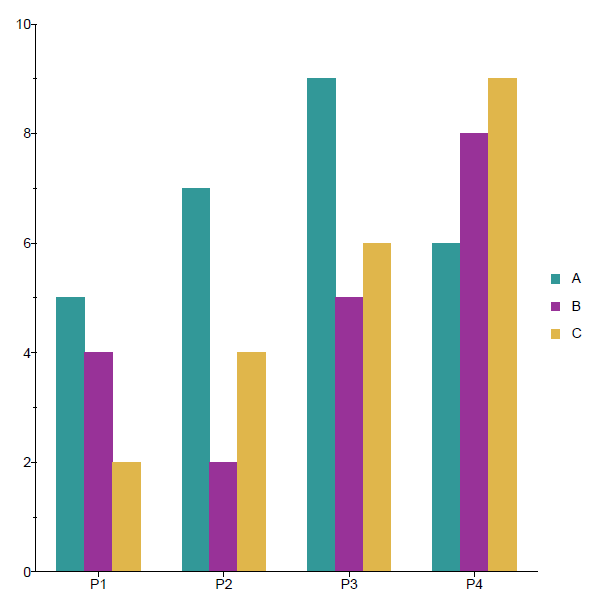
\includegraphics[scale=0.25]{figures/ch10/fig13}\caption{A column chart.}\label{fig:A-column-chart.}
\end{figure}

Scatter plots are a type of plot that uses Cartesian coordinates to
display values for typically two variables for a data set (Figure
\ref{fig:A-scatter-plot.}). Scatter charts are similar to line charts;
scatter charts only use numeric values for both the x-axis and y-axis,
while in line charts, the x-axis is not numeric. Series data for the
scatter plots can be either indexed or date/time. Core Suite provides
the \texttt{XYScatterSeries}\index{XYScatterSeries} for creating scatter plots, which you
learn about in the next chapter (Chapter \ref{sec:Scatter-Chart}).

\begin{figure}[h]
\centering

\includegraphics[scale=0.3]{figures/ch11/fig11}\caption{A scatter plot.}\label{fig:A-scatter-plot.}

\end{figure}

As you can see, DynamicPDF Core Suite for .NET provides many different
types of charts that you can add to your PDF documents.\marginnote{There are so many classes and options we can't possibly cover all
in this book. Consider the following two chapters more of a tutorial
on how to create charts using Core Suite. Refer to online API documentation
for more comprehensive class and properties listing.} But before discussing each particular chart type in detail, let's
first discuss the elements common to every chart. After discussing
the common elements of every chart, we can then examine the different
charts, beginning with the pie chart, bar chart, and column chart.
Then, in the next chapter, we delve further into charting by discussing
line and scatter charts. By the end of chapter \ref{chap:Charts-II}
you will know how to build all the charts offered by Core Suite. And
as I stated in the beginning of this chapter, I am certain you will
be impressed with the versatility and quality of the charts DynamicPDF
Core Suite for .NET offers.

\section{Chart Elements}

Let's begin our discussion of charting by first considering the common
elements every chart created using Core Suite must have when being
created. A  "chart" consists of a \texttt{Chart}\index{Chart}, one or more plot
areas, data series, an x-axis and y-axis, and legends.\sidenote{To avoid confusion, here on out we refer to a \texttt{Chart}\index{Chart} object
by its class name, and the created chart using lowercase.} All charts start with a \texttt{Chart}\index{Chart} instance and a \texttt{PlotArea}\index{PlotArea}
instance and are fundamental to understanding how to build a chart
using Core Suite.

\subsection{Chart}

All charts start with a \texttt{Chart}\index{Chart} class instance (your "canvas").\marginnote{When working through this chapter, before deciding you must create
custom instances of the different classes, consider if the default's
provided by Core Suite meets your requirements.} A \texttt{Chart}\index{Chart} instance has one or more plot areas (the "paint"
added to your "canvas"). Each plot area consists of one or more
data series (the "brush strokes" comprising the "paint").
The data series are what drives the visual display(s) of a chart's
data.

A \texttt{Chart}\index{Chart} has two constructor overloads, allowing you to specify
the chart's coordinates, dimensions, font, and text color. These properties
apply to all element used by a \texttt{Chart}\index{Chart} but can be overridden
by a chart's plot area and data series. A \texttt{Chart}\index{Chart} instance
can have one or more header and footer titles. And a \texttt{Chart}\index{Chart}
instance can have a title and subtitle, as can a plot area. You add
a title to a \texttt{Chart}\index{Chart} using the \texttt{Title}\index{Title} class combined
with the \texttt{Chart}\index{Chart} instance's \texttt{HeaderTitles}\index{HeaderTitles} and \texttt{FooterTitles}\index{FooterTitles}
properties, both of which define a collection of \texttt{Title}\index{Title} instances.
For example, let's create a pie chart that has a header and footer
title. 
\begin{marginfigure}

\includegraphics[scale=0.27]{figures/ch10/fig1}\caption{A simple pie chart.}\label{mar:A-simple-pie}

\end{marginfigure}

Listing \ref{lis:chart-simple-create} illustrates creating a simple
pie chart. To keep our discussion focused on only the \texttt{Chart}\index{Chart},
we ommit the source code for creating the plot area and data series.
You first create a \texttt{Chart}\index{Chart} instance and add two header titles
and a footer title. You also modify the \texttt{Chart}\index{Chart} instance's
background color - just to make its location and dimensions easily
visible. You then call \texttt{AddPlot}\index{AddPlot} (our user-defined method) to
add the plot and data series to the \texttt{Chart}\index{Chart} instance (omitted). 

You also add colors to the chart's elements so that the chart's layout
is clearly visible. The \texttt{Chart}\index{Chart} instance's background colors
illustrate the different chart elements: the light green is the chart's
background, while the plot area's background is tan (Figure \ref{mar:A-simple-pie}).

\bgroup\inputencoding{latin9}
\begin{lstlisting}[caption={Creating a simple chart.},label={lis:chart-simple-create},basicstyle={\small\ttfamily},breaklines=true]
using ceTe.DynamicPDF;
using ceTe.DynamicPDF.PageElements.Charting;
using ceTe.DynamicPDF.PageElements.Charting.Series;

namespace ChapterExamples.Chapters.ChapterTen
{
    public class SimpleChartExample
    {
        public static void Create(string outputPath)
        {
            Document doc = new();
            doc.Pages.Add(new Page(PageSize.Letter));

            float hght = doc.Pages[0].Dimensions.Height - doc.Pages[0].Dimensions.TopMargin * 2;
            float wdth = doc.Pages[0].Dimensions.Width - doc.Pages[0].Dimensions.RightMargin * 2;
 
            chart.BackgroundColor = RgbColor.LightGreen;
            chart.HeaderTitles.Add(new Title("Acme Corporation Item Report"));
            chart.HeaderTitles.Add(new Title("For Calendar Year 2021"));
            chart.HeaderTitles[1].FontSize = 10;
            chart.FooterTitles.Add(new Title("Copyright 2024"));
            chart.FooterTitles[0].FontSize = 8;

            AddPlot(chart, wdth, hght);
            doc.Pages[0].Elements.Add(chart);
            doc.Draw(outputPath + "chart-out.pdf");
        }

        private static void AddPlot(Chart chart, float wdth, float hght)
        {
            --- snip ---
        }
    }
}
\end{lstlisting}
\leavevmode\egroup

Notice that the chart in Figure \ref{mar:A-simple-pie} auto-sized
the plot area to fit the chart's bounds. It also added a legend and
placed it in what auto-layout determined as the best location. Core
Suite is smart enough to automatically layout charts using default
settings, but, as you will see later in this chapter, you can disable
auto-layout and manually layout a chart's elements if you wish.

\subsection{Plot Area}

After the \texttt{Chart}\index{Chart}, the \texttt{PlotArea}\index{PlotArea} is the most important
class in building a chart. A \texttt{Chart}\index{Chart} contains one or more plot
areas. A \texttt{PlotArea}\index{PlotArea} contains one or more series and is the
area in the chart where the series is plotted. A \texttt{Chart}\index{Chart} instance
contains a \texttt{PrimaryPlotArea}\index{PrimaryPlotArea} by default but can override the
primary plot area by creating your own or by modifying the primary
plot area dimensions.\marginnote{Do not be confused if you see code referring to a plot area by a Chart
instance's PrimaryPlotArea or PlotAreas[n]; both refer to a plot area. PlotArea[0] is the same as
the PrimaryPlotArea unless you replace it with your own custom
plot area. You can also add multiple plot areas to a chart.}

Every plot area has an x-axis and y-axis and the \texttt{PlotArea}\index{PlotArea}
class has properties for modifying its appearance, dimensions, placement,
titles, and properties for setting its data series and axes. If you
wish to create a plot area rather than using the primary plot area,
create a new plot area and then add it to the \texttt{Chart}\index{Chart} instance's
\texttt{PlotAreas}\index{PlotAreas} collection (\texttt{PlotAreaList}\index{PlotAreaList}). The \texttt{Chart}\index{Chart}
then uses that plot area rather than the primary plot area.

Now, let's add the \texttt{AddPlot}\index{AddPlot} method's code to the previous
example and use the \texttt{PrimaryPlotArea}\index{PrimaryPlotArea} to modify the chart's
appearance (Listing \ref{lis:Adding-a-plot}). Although we have not
discussed adding a data series with a pie chart, we include it here
to illustrate creating a plot area. 

Notice you do not create the plot area but instead rely on the \texttt{Chart}\index{Chart}
instance's primary plot area. You also add top and bottom titles to
the plot area (Figure \ref{mar:A-backprimary-plot}) and header and
footer titles to the \texttt{Chart}\index{Chart}. You center the plot area's titles
which centers them on the plot area while the \texttt{Chart}\index{Chart} instance's
titles are centered on the chart. Also notice you add a subtitle to
the plot area's top title. You are not limited to a single title,
as you do in~Listing \ref{lis:Adding-a-plot}; both the plot area
and the \texttt{Chart}\index{Chart} instance's title are collections of \texttt{Title}\index{Title}
instances and allow you to add multiple titles, where each title is
placed below the previous title. 
\begin{figure}

\includegraphics[scale=0.50]{figures/ch10/fig2}\caption{A primary plot area with a title and background color.}\label{mar:A-backprimary-plot}

\end{figure}

\bgroup\inputencoding{latin9}
\begin{lstlisting}[caption={Adding a plot area to a chart.},label={lis:Adding-a-plot},basicstyle={\small\ttfamily},breaklines=true]
private static void AddPlot(Chart chart, float wdth, float hght)
{
   chart.PrimaryPlotArea.BackgroundColor = RgbColor.Tan;
   chart.PrimaryPlotArea.TopTitles.Add(new Title("The Plot Area Top"));
   chart.PrimaryPlotArea.BottomTitles.Add(new Title("The Plot Area Bottom"));         
   PieSeries pieSeries = new PieSeries();
   ScalarDataLabel dataLabel = new ScalarDataLabel(true, false, false);
   pieSeries.DataLabel = dataLabel;

   PieSeriesElement pe1 = new(10, "A", RgbColor.Navy);
   PieSeriesElement pe2 = new(20, "B", RgbColor.Red);

   pieSeries.Elements.Add(pe1);
   pieSeries.Elements.Add(pe2);
   chart.PrimaryPlotArea.Series.Add(pieSeries);
}
\end{lstlisting}
\leavevmode\egroup


\subsection{Legend}

Data variables appearing in a chart usually contain a key visually
identifying those variables. This key is called a legend and consists
of a list of variables and an example showing how those variables
appear in the data series. 

Core Suite provides the \texttt{Legend}\index{Legend} class for creating legends
for your data series. A \texttt{Chart}\index{Chart} instance contains a \texttt{Legends}\index{Legends}
property, which is a collection (\texttt{LegendList}\index{LegendList}) of one or more
\texttt{Legend}\index{Legend} instances. Create a legend by calling a legend list's
\texttt{Add} method. Of course, as with a default plot area, you are
not required to create a \texttt{Legend}\index{Legend}, as if you do not create
one, then a default legend is created. For example, in Listing \ref{lis:Adding-a-plot}
we do not specify a legend. Instead, the series element values are
automatically added to the default legend. The legend is then automatically
added to the chart (Figure \ref{mar:A-backprimary-plot}).

The \texttt{Legend}\index{Legend} class has numerous properties for customizing
its appearance, positioning, and dimensions. You can also control
legend placement using the \texttt{LegendList}\index{LegendList} instance's \texttt{Placement}\index{Placement}
property.

\bgroup\inputencoding{latin9}
\begin{lstlisting}[basicstyle={\small\ttfamily},breaklines=true]
chart.Legends.Placement = LegendPlacement.BottomLeft;
\end{lstlisting}
\leavevmode\egroup
Placement values are \texttt{BottomCenter}, \texttt{BottomLeft}, \texttt{BottomRight},
\texttt{LeftCenter}, \texttt{RightCenter}, \texttt{TopCenter}, \texttt{TopLeft},
and \texttt{TopRight}. By default, the \texttt{LegendPlacement}\index{LegendPlacement} is
set to \texttt{RightCenter}. 

When adding a \texttt{Legend}\index{Legend} to a series, the series's \texttt{Name}
property is the text added to the legend. You can also customize a
legend's appearance and labels, as Listing \ref{lis:Customizing-a-legend.}
illustrates. For example, assume in Listing \ref{lis:Adding-a-plot},
just below the \texttt{AddPlot}\index{AddPlot} method, we add a call to the method
in Listing \ref{lis:Customizing-a-legend.}. The method modifies the
legend's placement, label text, and font size. The first label's text
is modified and second label's font size is increased. The legend
is also placed on the \texttt{Chart}\index{Chart} instance's lower left corner
(Figure \ref{fig:Customizing-a-legend.}). Although not the most professional
appearing chart, you get the idea, as the text and font size are both
changed.
\begin{figure}

\includegraphics[scale=0.55]{figures/ch10/fig3}\caption{Customizing a legend.}\label{fig:Customizing-a-legend.}

\end{figure}

\bgroup\inputencoding{latin9}
\begin{lstlisting}[caption={Customizing a legend.},label={lis:Customizing-a-legend.},basicstyle={\small\ttfamily},breaklines=true]
private static void CustomizeLegend(Chart chart, PieSeries series)
{
    chart.Legends.Placement = LegendPlacement.BottomLeft;
    chart.Legends[0].LegendLabelList[0].Text += " Value";
    chart.Legends[0].LegendLabelList[1].FontSize = 24;
}
\end{lstlisting}
\leavevmode\egroup


\subsection{Summary - Common Elements}

Do not be misled by the brevity given to the \texttt{Chart} class,
plot areas, and legend in this chapter. Core Suite allows extensive
customization of both, refer to the individual classes in this book's
appendix for more details and listings of the numerous properties
and methods available for these classes. However, when you start building
your chart remember the following points.
\begin{enumerate}
\item A Chart contains one or more plot areas.
\item A Chart contains one or more legends.
\item If you do not provide a plot area, then the Chart instance automatically
creates a primary plot area.
\item If you do not provide a legend, then the Chart instance automatically
creates a default legend. 
\item By default, a \texttt{Chart} automatically best lays out your chart
on your PDF document.\sidenote{The Chart instance's \texttt{AutoLayout}\index{AutoLayout} property is set to \texttt{true}
by default.}
\end{enumerate}
Now that we understand these charting fundamentals, let's consider
pie charts, bar charts, and column charts. Then in the next chapter,
we return to these charting fundamentals by discussing x and y axes,
as well as discussing line, area, and scatter charts.

\section{Pie Charts}\label{sec:Pie-Charts}

Pie charts divide a circle into different "slices" depending on
the data represented in each slice. Each slice displays its related
data. Core Suite provides the \texttt{PieSeries}\index{PieSeries} class for creating
pie charts. To create a chart, you first create a \texttt{Chart}\index{Chart} instance
and then a \texttt{PieSeries}\index{PieSeries} which you add to the plot area. A \texttt{PieSeries}\index{PieSeries}
instance contains a \texttt{PieSeriesElementList}\index{PieSeriesElementList}. The \texttt{PieSeriesElementList}\index{PieSeriesElementList}
contains one or more \texttt{PieSeriesElement}\index{PieSeriesElement} instances. You add
these elements to the series. A \texttt{PieSeriesElement}\index{PieSeriesElement} consists
of the data value and the value's name. You can customize the \texttt{PieSeries}\index{PieSeries}
class and each \texttt{PieSeriesElement}\index{PieSeriesElement} class's appearance, changing
things like the slice color, border appearance, name, and legend.
When creating a pie series, you must also use a \texttt{ScalarDataLabel}\index{ScalarDataLabel}
to define the data labels identifying the slices. 

Listing \ref{lis:A-pie-chart} illustrates creating a pie chart. After
creating a \texttt{Chart}\index{Chart} instance, you next create a new \texttt{PieSeries}\index{PieSeries}
instance and define the \texttt{ScalarDataLabel}\index{ScalarDataLabel}. The \texttt{ScalarDataLabel}\index{ScalarDataLabel}
class's constructor takes three booleans which initialize the series
to show the data values but not the percentages or element names.
You then add the data series to the chart's \texttt{PrimaryPlotArea}\index{PrimaryPlotArea}. 

After creating a \texttt{Chart}\index{Chart} instance and adding a series to the
\texttt{PrimaryPlotArea}\index{PrimaryPlotArea}, you create four \texttt{PieSeriesElement}\index{PieSeriesElement}
instances and add data to each element. You then add the elements to
the series element list. Finally, you add the series to the \texttt{Chart}\index{Chart},
and the \texttt{Chart}\index{Chart} to the page. Figure \ref{fig:A-simple-pie}
illustrates the resulting pie chart.

\bgroup\inputencoding{latin9}
\begin{lstlisting}[caption={A pie chart example.},label={lis:A-pie-chart},basicstyle={\small\ttfamily},breaklines=true]
using ceTe.DynamicPDF;
using ceTe.DynamicPDF.PageElements.Charting;
using ceTe.DynamicPDF.PageElements.Charting.Series;

namespace ChapterExamples.Chapters.ChapterTen
{
    public class PieChartExample
    {
        public static void Create(string outputPath)
        {
            Document doc = new();
            doc.Pages.Add(new Page(PageSize.Letter, PageOrientation.Landscape));

            Chart chart = new Chart(0, 0, 500, 500);

            PieSeries pieSeries = new PieSeries();
            ScalarDataLabel dataLbl = new ScalarDataLabel(true, false, false);
            pieSeries.DataLabel = dataLbl;

            chart.PrimaryPlotArea.Series.Add(pieSeries);

            PieSeriesElement pe1 = new(10, "A", RgbColor.Red);
            PieSeriesElement pe2 = new(20, "B", RgbColor.Blue);
            PieSeriesElement pe3 = new(13, "C", RgbColor.Yellow);
            PieSeriesElement pe4 = new(17, "D", RgbColor.Green);

            pieSeries.Elements.Add(pe1);
            pieSeries.Elements.Add(pe2);
            pieSeries.Elements.Add(pe3);
            pieSeries.Elements.Add(pe4);

            doc.Pages[0].Elements.Add(chart);
            doc.Draw(outputPath + "simplest-pie-chart-out.pdf");
        }
    }
}
\end{lstlisting}
\leavevmode\egroup
\begin{figure}[h]
\raggedright
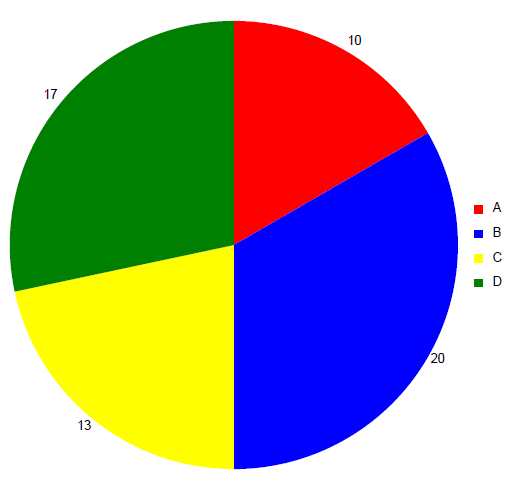
\includegraphics[scale=0.59]{figures/ch10/fig15}\caption{A simple pie chart.}\label{fig:A-simple-pie}

\end{figure}

As Figure \ref{fig:A-simple-pie} illustrates, each slice was labeled
with its value. Because the \texttt{ScalarDataLabel}\index{ScalarDataLabel} instance's constructor
was initialized to only show the slice's value, both name and percentage
were omitted. The default legend automatically added each \texttt{PieSeriesElement}\index{PieSeriesElement}
instance's name to the legend, and both the legend and slice were
assigned the corresponding element's defined color.

\section{Bar Chart}\label{sec:Bar-Chart}

While a pie series presents data in slices, a bar chart presents categorical
data using rectangular bars with heights or lengths proportional to
the values they represent. DynamicPDF Core Suite for .NET supports
three types of bar charts: normal, stacked, and 100\% stacked. Each
type can use either indexed data or date/time data. Table \ref{tab:bar-chart-Core-Suite-classes-1}
lists the classes available for creating bar charts.

\begin{table}
\raggedright
\begin{tabular}{p{0.45\textwidth}p{0.5\textwidth}}
\toprule 
{\scriptsize Series Class} & {\scriptsize Element Class}\tabularnewline
\midrule
{\scriptsize\texttt{IndexedBarSeries}} & {\scriptsize\texttt{-}}\tabularnewline
{\scriptsize\texttt{DateTimeBarSeries}} & {\scriptsize\texttt{-}}\tabularnewline
{\scriptsize\texttt{IndexedStackedBarSeries}} & {\scriptsize\texttt{IndexedStackedBarSeriesElement}}\tabularnewline
{\scriptsize\texttt{DateTimeStackedBarSeries}} & {\scriptsize\texttt{DateTimeStackedBarSeriesElement}}\tabularnewline
{\scriptsize\texttt{Indexed100PercentStackedBarSeries}} & {\scriptsize\texttt{Indexed100PercentStackedBarSeriesElement}}\tabularnewline
{\scriptsize\texttt{DateTime100PercentStackedBarSeries}} & {\scriptsize\texttt{DateTime100PercentStackedBarSeriesElement}}\tabularnewline
\bottomrule
\end{tabular}\caption{Bar chart classes.}\label{tab:bar-chart-Core-Suite-classes-1}
\end{table}


\subsection{Normal Indexed Data}

Normal indexed bar charts use one or more \texttt{IndexedBarSeries}\index{IndexedBarSeries}
instances to add data to a plot area. Indexed data is added to the
y-axis while numeric data is added to the x-axis. Unlike a pie series,
which contains only one series, a bar chart's plot area contains multiple
series, where each series contains the related data. 

Listing \ref{lis:A-simple-bar} illustrates creating a bar chart.
First, you create three \texttt{IndexedBarSeries}\index{IndexedBarSeries} instances. You then
add data to the \texttt{Values} collection of each series using the
series instance's \texttt{Add}\index{Add} method. You add each series to the \texttt{Chart}\index{Chart}
instance's primary plot area. After adding each series, you create
the y-axis labels using \texttt{IndexedYAxisLabel}\index{IndexedYAxisLabel} instances. As each
series has four values, the \texttt{YAxis}\index{YAxis} creates a label corresponding
to the value's position in the data array. For instance, for series
A, the values 4, 5, 8, and 2 corresponds to positions 0, 1, 2, and
3. The same relationship holds true for the values of B and C.\sidenote{If you were to omit adding the y-axis labels, then Core Suite assigns
default labels using the position of each series's value (Figure \ref{mar:indbarOmitting-labels-for}).}

Note that you only add labels for the first series, as subsequent series
added to the plot have the same value meanings. The result is a bar
chart with three series and four values (Figure \ref{mar:bar-chart-A-simple-bar}).
\begin{figure}
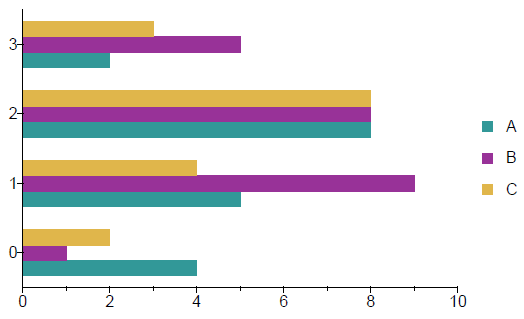
\includegraphics[scale=0.55]{figures/ch10/fig22}\caption{Omitting labels for y-axis.}\label{mar:indbarOmitting-labels-for}
\end{figure}

\bgroup\inputencoding{latin9}
\begin{lstlisting}[caption={A simple bar chart with indexed data.},label={lis:A-simple-bar},basicstyle={\small\ttfamily},breaklines=true]
using ceTe.DynamicPDF;
using ceTe.DynamicPDF.PageElements.Charting;
using ceTe.DynamicPDF.PageElements.Charting.Axes;
using ceTe.DynamicPDF.PageElements.Charting.Series;

namespace ChapterExamples.Chapters.ChapterTen
{
    public class BarchartExample
    {
        public static void Create(string outputPath)
        {
            Document doc = new Document();
            doc.Pages.Add(new Page(PageSize.Letter));

            Chart chart = new Chart(0, 0, 400, 230);
            IndexedBarSeries barSeries = new IndexedBarSeries("A");
            barSeries.Values.Add(new float[] { 4, 5, 8, 2 });
            IndexedBarSeries barSeries2 = new IndexedBarSeries("B");
            barSeries2.Values.Add(new float[] { 1, 9, 8, 5 });
            IndexedBarSeries barSeries3 = new IndexedBarSeries("C");
            barSeries3.Values.Add(new float[] { 2, 4, 8, 3 });
            
            chart.PrimaryPlotArea.Series.Add(barSeries);
            chart.PrimaryPlotArea.Series.Add(barSeries2);
            chart.PrimaryPlotArea.Series.Add(barSeries3);

            barSeries.YAxis.Labels.Add(new IndexedYAxisLabel("P1", 0));
            barSeries.YAxis.Labels.Add(new IndexedYAxisLabel("P2", 1));
            barSeries.YAxis.Labels.Add(new IndexedYAxisLabel("P3", 2));
            barSeries.YAxis.Labels.Add(new IndexedYAxisLabel("P4", 3));

            doc.Pages[0].Elements.Add(chart);
            doc.Draw(outputPath + "simple-bar-chart-out.pdf");
        }
    }
}
\end{lstlisting}
\leavevmode\egroup

\begin{figure}

\includegraphics[scale=0.55]{figures/ch10/fig6}\caption{A simple bar chart added to a PDF document.}\label{mar:bar-chart-A-simple-bar}
\end{figure}


\subsection{Normal Date/Time Data}

You use a date-time series with a bar chart by creating one
or more \texttt{DateTimeBarSeries}\index{DateTimeBarSeries} instances and then for each adding
the value and date/time as a \texttt{DateTimeBarValue}\index{DateTimeBarValue} to the element's
\texttt{DateTimeBarValueList}\index{DateTimeBarValueList} (\texttt{Values} property).

Listing \ref{lis:A-simple-bar-datetime1} illustrates using a date/time
series to create a bar chart. First, you create three \texttt{DateTimeBarSeries}\index{DateTimeBarSeries}
instances and add \texttt{DateTimeBarValue}\index{DateTimeBarValue} instances to the \texttt{Values}
list of each bar series. Next you add each series to the plot area.
Then you set the y-axis format label so each label shows the complete
date. Note that Listing \ref{lis:A-simple-bar-datetime1} also illustrates
adding a value by creating a \texttt{DateTimeBarValue}\index{DateTimeBarValue} instance for
the fourth value of series A and then adding the instance to the \texttt{Values}
list (just to reinforce that the Add method is overloaded to also
take a a \texttt{DateTimeBarValue}\index{DateTimeBarValue} and not only a combination of a
numeric and date/time value). Figure \ref{mar:A-simple-bar} illustrates
the resulting bar chart.
\begin{figure}

\includegraphics[scale=0.45]{figures/ch10/fig7}\caption{A simple bar chart with date/time data.}\label{mar:A-simple-bar}
\end{figure}
\bgroup\inputencoding{latin9}
\begin{lstlisting}[caption={A simple bar chart with date/time data.},label={lis:A-simple-bar-datetime1},basicstyle={\small\ttfamily},breaklines=true]
using ceTe.DynamicPDF;
using ceTe.DynamicPDF.PageElements.Charting;
using ceTe.DynamicPDF.PageElements.Charting.Axes;
using ceTe.DynamicPDF.PageElements.Charting.Series;
using System;

namespace ChapterExamples.Chapters.ChapterTen
{
    public class BarchartExample
    {
        public static void Create(string outputPath)
        {
            Document doc = new Document();
            doc.Pages.Add(new Page(PageSize.Letter));

            Chart chart = new Chart(0, 0, 500, 400);

            DateTimeBarSeries barSeries = new DateTimeBarSeries("A");
            barSeries.Values.Add(5, new DateTime(2017, 1, 1));
            barSeries.Values.Add(7, new DateTime(2017, 2, 9));
            barSeries.Values.Add(9, new DateTime(2017, 3, 7));
            DateTimeBarValue value = new(6, new DateTime(2015, 4, 1));
            barSeries.Values.Add(value);

            DateTimeBarSeries barSeries2 = new DateTimeBarSeries("B");
            barSeries2.Values.Add(4, new DateTime(2012, 1, 1));
            barSeries2.Values.Add(2, new DateTime(2017, 2, 9));
            barSeries2.Values.Add(5, new DateTime(2017, 3, 7));
            barSeries2.Values.Add(8, new DateTime(2017, 4, 1));

            DateTimeBarSeries barSeries3 = new DateTimeBarSeries("C");
            barSeries3.Values.Add(2, new DateTime(2017, 1, 1));
            barSeries3.Values.Add(4, new DateTime(2017, 2, 9));
            barSeries3.Values.Add(6, new DateTime(2017, 3, 7));
            barSeries3.Values.Add(9, new DateTime(2017, 4, 1));

            chart.PrimaryPlotArea.Series.Add(barSeries);
            chart.PrimaryPlotArea.Series.Add(barSeries2);
            chart.PrimaryPlotArea.Series.Add(barSeries3);

            barSeries.YAxis.LabelFormat = "D";

            Title title3 = new Title("Items");
            barSeries.XAxis.Titles.Add(title3);

            doc.Pages[0].Elements.Add(chart);
            doc.Draw(outputPath + "simple-bar-date-time-chart-out.pdf");
        }
    }
}
\end{lstlisting}
\leavevmode\egroup

As Figure \ref{mar:A-simple-bar} illustrates, the series is organized
by date/time on the y-axis and values on the x-axis. Because the y-axis
label format was set to ``D'', the date/time values are displayed
as the day of the week and complete date.

You can change what's displayed on the y-axis using a \texttt{DateTimeType}\index{DateTimeType}.
Valid types are \texttt{Day}, \texttt{Hour}, \texttt{Minute}, \texttt{Month},
\texttt{Second}, \texttt{Undefined}, and \texttt{Year}. For instance,
changing

\bgroup\inputencoding{latin9}
\begin{lstlisting}[basicstyle={\small\ttfamily}]
barSeries.YAxis.LabelFormat = "D";
\end{lstlisting}
\leavevmode\egroup
to\bgroup\inputencoding{latin9}
\begin{lstlisting}[basicstyle={\small\ttfamily},breaklines=true]
 barSeries.YAxis.DateTimeType = DateTimeType.Year;
\end{lstlisting}
\leavevmode\egroup
in Listing \ref{lis:A-simple-bar-datetime1} creates a bar chart like
Figure \ref{mar:bar-chart-Changing-the-date/time}, where the y-axis
is labeled with the year values rather than complete date.
\begin{figure}
\raggedright
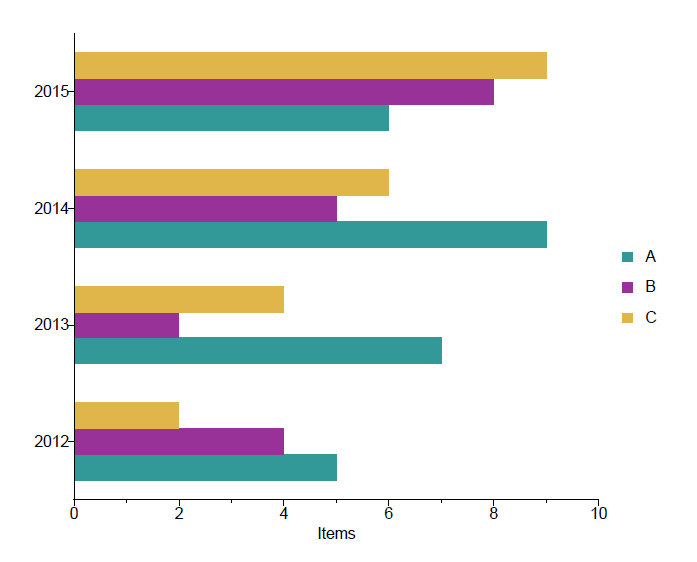
\includegraphics[scale=0.5]{figures/ch10/fig8}\caption{Changing the date/time type for a bar chart.}\label{mar:bar-chart-Changing-the-date/time}
\end{figure}


\subsection{Stacked Indexed Data}\label{subsec:Stacked-Indexed-Data}

A stacked bar chart displays its series values one on top of the other
and represents and compares segments of a whole. A stacked bar chart
divides one or more bars into multiple segments. Each bar is a different
category and each segment are the values represented. For example,
in Figure \ref{fig:Stacked-bar-chart}, P1, P2, P3, and P4 are the
categories while A, B, and C are the values represented.The values
are displayed stacked, and so the x-axis values represented are cumulative. 

Core Suite provides the \texttt{IndexedStackedBarSeries}\index{IndexedStackedBarSeries} class for
creating stacked bar charts. Unlike the normal indexed and date/time
bar charts, rather than creating multiple series and adding data values
to each series, you instead create a single series and then add values
to multiple \texttt{IndexedStackedBarSeriesElement}\index{IndexedStackedBarSeriesElement} instances. Each
element instance contains the values and positions for the data to
chart. You add the created element instances to the single series.
There is only one series instance and not multiple series.\sidenote{Although nothing prevents you from adding multiple stacked series
to the same plot area, the results are not visually intuitive and
you should stick to one series per plot area.} Instead this class uses a collection of \texttt{IndexedStackedBarSeriesElement}\index{IndexedStackedBarSeriesElement}
instances plotted as a \texttt{StackedBarSeries}\index{StackedBarSeries} in indexed order.
An \texttt{IndexedStackedBarSeries}\index{IndexedStackedBarSeries} uses the \texttt{IndexedXAxis}\index{IndexedXAxis}
class to represent the x-axis and the \texttt{NumericYAxis}\index{NumericYAxis} to represent
the y-axis.

Listing \ref{lis:Stacked-bar-chart} illustrates creating a stacked
bar chart. First, you create an \texttt{IndexedStackedBarSeries}\index{IndexedStackedBarSeries} instance
and three \texttt{IndexedStackBarSeriesElement}\index{IndexedStackBarSeriesElement} instances containing
the data values for each element instance. Note that the position
determines the y-axis value, so for the series created in Listing
\ref{lis:Stacked-bar-chart} you have the following two-dimensional
array where the column is the y-axis category and the row is values
represented.

\[
\begin{array}{cccc}
5 & 7 & 9 & 6\\
4 & 2 & 5 & 8\\
2 & 4 & 6 & 9
\end{array}
\]
Row one corresponds to A, row two corresponds to B, and row three
corresponds to C. Column zero corresponds with the first value in
A, B, and C. Columns one, two, and three correspond with the second,
third, and fourth values of A, B, and C.

In Listing \ref{lis:Stacked-bar-chart} you further illustrate value/position
by creating an \texttt{IndexedStackedBarValue}\index{IndexedStackedBarValue} instance to indicate
the value and position of the first value in \texttt{A} rather than
setting the values directly by the \texttt{Values} collection's \texttt{Add}
method. In this \texttt{IndexedStackedBarValue}\index{IndexedStackedBarValue} instance, five is
the value and zero is the position. You then add three more values
to \texttt{A} as an array where 7 is position one, 9 is position two,
and 6 is position three. You add all values at once as an array for
\texttt{B} and \texttt{C}. After creating the element instances, Listing
\ref{lis:Stacked-bar-chart} adds them to the series and then the
series to the \texttt{Chart} instance's primary plot area. 

You also add labels to the positions represented by the y-axis and
so rather than displaying 0, 1, 2, and 3 for the y-axis, it displays
P1, P2, P3, and P4. Figure \ref{fig:Stacked-bar-chart} illustrates
the resulting chart.
\begin{figure}
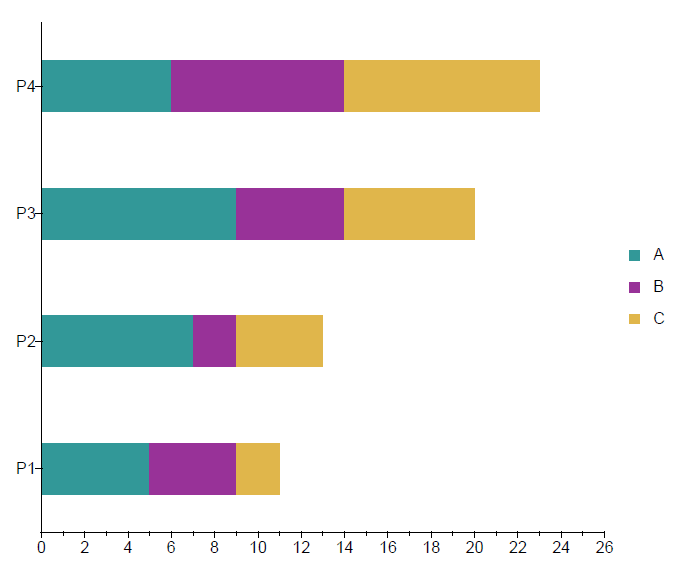
\includegraphics[scale=0.495]{figures/ch10/fig9}\caption{Stacked bar chart with indexed data example.}\label{fig:Stacked-bar-chart}
\end{figure}

\bgroup\inputencoding{latin9}
\begin{lstlisting}[caption={Stacked bar chart with indexed data example.},label={lis:Stacked-bar-chart},basicstyle={\small\ttfamily},breaklines=true]
using ceTe.DynamicPDF;
using ceTe.DynamicPDF.PageElements.Charting;
using ceTe.DynamicPDF.PageElements.Charting.Axes;
using ceTe.DynamicPDF.PageElements.Charting.Series;
using System;

namespace ChapterExamples.Chapters.ChapterTen
{
    public class BarchartExample
    {
        public static void Create(string outputPath)
        {
            Document doc = new Document();
            doc.Pages.Add(new Page(PageSize.Letter));
            Chart chart = new Chart(0, 0, 500, 400);

            IndexedStackedBarSeries stackedBarSeries = new IndexedStackedBarSeries();
            IndexedStackedBarSeriesElement se = new IndexedStackedBarSeriesElement("A");
            IndexedStackedBarValue sbv = new(5, 0);
            se.Values.Add(sbv);
            se.Values.Add(new float[] {7, 9, 6 });

            IndexedStackedBarSeriesElement se2 = new IndexedStackedBarSeriesElement("B");
            se2.Values.Add(new float[] { 4, 2, 5, 8 });
            IndexedStackedBarSeriesElement se3 = new IndexedStackedBarSeriesElement("C");
            se3.Values.Add(new float[] { 2, 4, 6, 9 });

            stackedBarSeries.Add(se);
            stackedBarSeries.Add(se2);
            stackedBarSeries.Add(se3);

            chart.PrimaryPlotArea.Series.Add(stackedBarSeries);

            stackedBarSeries.YAxis.Labels.Add(new IndexedYAxisLabel("P1", 0));
            stackedBarSeries.YAxis.Labels.Add(new IndexedYAxisLabel("P2", 1));
            stackedBarSeries.YAxis.Labels.Add(new IndexedYAxisLabel("P3", 2));
            stackedBarSeries.YAxis.Labels.Add(new IndexedYAxisLabel("P4", 3));
            
            doc.Pages[0].Elements.Add(chart);
            doc.Draw(outputPath + "simple-bar-indexed-stacked-chart-out.pdf");
        }
    }
}
\end{lstlisting}
\leavevmode\egroup

The first bar displays item \texttt{A}, \texttt{B}, and \texttt{C}
for period one (\texttt{P1}), while the second for \texttt{P2}, the
third for \texttt{P3}, and the fourth for \texttt{P4}. \texttt{P1}
corresponds with the {[}0{]} data value for each series, \texttt{P2}
the {[}1{]} data value, \texttt{P3} the {[}2{]} value, and \texttt{P4}
the {[}3{]} value. So, for example, \texttt{P1} displays \texttt{A}'s
value of 5 as the teal portion of the bar, \texttt{B}'s value of 7
as the purple portion of the bar between 5 and 9, and \texttt{C}'s
value of 2 as the yellow portion of the bar between 9 and 11.

\subsection{Stacked Date/Time Data}

A stacked date/time bar series, like a stacked indexed bar series,
shows a larger value set divided into smaller categories and compares
those categories across the value sets. When using a time series,
the date/time series values are the category positions while the values
are the represented data. So for example, with the following data
set, the categories are the dates while the value type is A, B, and
C (Table \ref{mar:Values-by-category.}).
\begin{margintable}
\begin{tabular}{cccc}
\toprule 
 & A & B & C\tabularnewline
\midrule
1/1/2012 & 5 & 4 & 2\tabularnewline
2/9/2013 & 7 & 2 & 4\tabularnewline
3/7/2014 & 9 & 5 & 6\tabularnewline
4/1/2015 & 6 & 8 & 9\tabularnewline
\bottomrule
\end{tabular}

\medskip{}
\caption{Values by category.}\label{mar:Values-by-category.}

\end{margintable}

Core suite provides the \texttt{DateTimeStackedBarSeries}\index{DateTimeStackedBarSeries} class for
creating a stacked date/time chart. A \texttt{DateTimeStackedBarSeries}\index{DateTimeStackedBarSeries}
instance is comprised of multiple \texttt{DateTimeStackedBarSeriesElement}\index{DateTimeStackedBarSeriesElement}
class instances. Each element contains a \texttt{Values} property
where you add one or more values using the \texttt{Add} method. The
\texttt{Values} property is a \texttt{DateTimeStackedBarValueList}\index{DateTimeStackedBarValueList}
comprised of one or more \texttt{DateTimeStackedBarValue}\index{DateTimeStackedBarValue} instances.

Listing \ref{lis:A-date/time-stacked} illustrates a date/time stacked
bar chart. First, you create a new \texttt{DateTimeStackedBarSeries}\index{DateTimeStackedBarSeries}
instance. Then, you create three \texttt{DateTimeStackedBarSeriesElement}\index{DateTimeStackedBarSeriesElement}
instances and add \texttt{DateTimeStackedBarValue}\index{DateTimeStackedBarValue} instances to the
element's \texttt{DateTimeStackedBarValueList}\index{DateTimeStackedBarValueList} instance using the
\texttt{Add} method. As with Listing \ref{lis:Stacked-bar-chart},
the first element, \texttt{A}, adds the first value explicitly using
a \texttt{DateTimeStackedBarValue}\index{DateTimeStackedBarValue} instance. \texttt{A} then adds
the remaining values using the \texttt{Add} method's overload that
takes a scalar value and a date/time. Finally, you add the elements
to the series and the series to the chart's primary plot area. The
results is a stacked date/time bar chart (Figure \ref{mar:A-date/time-stacked}).
\begin{figure}
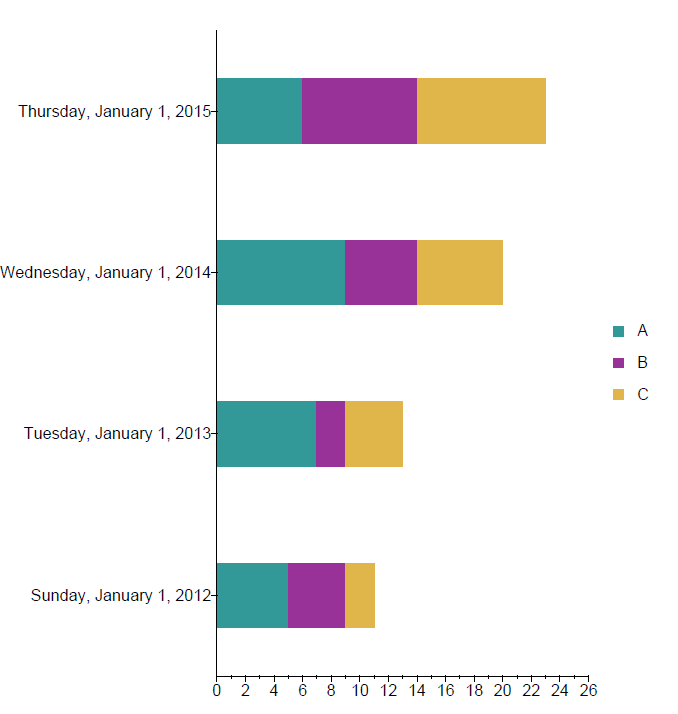
\includegraphics[scale=0.5]{figures/ch10/fig10}\caption{A date/time stacked bar chart.}\label{mar:A-date/time-stacked}
\end{figure}
\bgroup\inputencoding{latin9}
\begin{lstlisting}[caption={A date/time stacked bar chart.},label={lis:A-date/time-stacked},basicstyle={\small\ttfamily},breaklines=true]
using ceTe.DynamicPDF;
using ceTe.DynamicPDF.PageElements.Charting;
using ceTe.DynamicPDF.PageElements.Charting.Axes;
using ceTe.DynamicPDF.PageElements.Charting.Series;
using ceTe.DynamicPDF.PageElements.Charting.Values;
using System;

namespace ChapterExamples.Chapters.ChapterTen
{
    public class BarchartExample
    {
        public static void Create(string outputPath)
        {
            Document doc = new Document();
            doc.Pages.Add(new Page(PageSize.Letter));
            Chart chart = new Chart(0, 0, 500, 500);

            DateTimeStackedBarSeries stackedBarSeries = new DateTimeStackedBarSeries();
            DateTimeStackedBarSeriesElement se = new DateTimeStackedBarSeriesElement("A");
            DateTimeStackedBarValue stbv = new(5, new DateTime(2012, 1, 1));
            se.Values.Add(stbv);
            se.Values.Add(7, new DateTime(2013, 2, 9));
            se.Values.Add(9, new DateTime(2014, 3, 7));
            se.Values.Add(6, new DateTime(2015, 4, 1));

            DateTimeStackedBarSeriesElement se2 = new DateTimeStackedBarSeriesElement("B");
            se2.Values.Add(val);
            DateTimeStackedBarValue val = new(4, new DateTime(2012, 1, 1));
            se2.Values.Add(2, new DateTime(2013, 2, 9));
            se2.Values.Add(5, new DateTime(2014, 3, 7));
            se2.Values.Add(8, new DateTime(2015, 4, 1));

            DateTimeStackedBarSeriesElement se3 = new DateTimeStackedBarSeriesElement("C");
            se3.Values.Add(2, new DateTime(2012, 1, 1));
            se3.Values.Add(4, new DateTime(2013, 2, 9));
            se3.Values.Add(6, new DateTime(2014, 3, 7));
            se3.Values.Add(9, new DateTime(2015, 4, 1));

            stackedBarSeries.Add(se);
            stackedBarSeries.Add(se2);
            stackedBarSeries.Add(se3);
                        
            chart.PrimaryPlotArea.Series.Add(stackedBarSeries);
            stackedBarSeries.YAxis.LabelFormat = "D";
            doc.Pages[0].Elements.Add(chart);
            doc.Draw(outputPath + "date-time-bar-stacked-chart-out.pdf");
        }
    }
}
\end{lstlisting}
\leavevmode\egroup

\subsection{Stacked 100\% Indexed Data}

A stacked 100\% indexed bar series, like the previous two stacked
bar series we examined, shows values divided into smaller categories
and compares the categories across them, only they are stacked as
a percentage of the total. Core Suite provides the \texttt{Indexed100PercentStackedBarSeries}\index{Indexed100PercentStackedBarSeries}
to create a stacked 100\% bar series and consists of\linebreak \texttt{Indexed100PercentStackedBarSeriesElement}\index{Indexed100PercentStackedBarSeriesElement} instances.
Each element instance contains one or more values. Like the other
two stacked series, the categories are the y-axis while the values
are the x-xis.\sidenote{Refer to Section \ref{subsec:Stacked-Indexed-Data} for a more in-depth
description of value/categories and how they are used to create a
stacked bar chart.}

In Listing \ref{lis:A-stacked-100=000025} you create a stacked 100\%
indexed bar chart. First, you create an \texttt{Indexed100PercentStackedBarSeries}\index{Indexed100PercentStackedBarSeries}
instance followed by three \texttt{Indexed100PercentStackedBarSeriesElement}\index{Indexed100PercentStackedBarSeriesElement}
instances and add values to the each of the instances. After adding
the values, you add the element instances to the series.

After adding the elements to the series, you then add the series to
the \texttt{Chart} instance's primary plot area. You then add the y-axis
category values so that we ensure the labels are displayed rather
than only the position being displayed. Figure \ref{mar:A-stacked-100=000025}
illustrates the resulting chart.

\begin{figure}
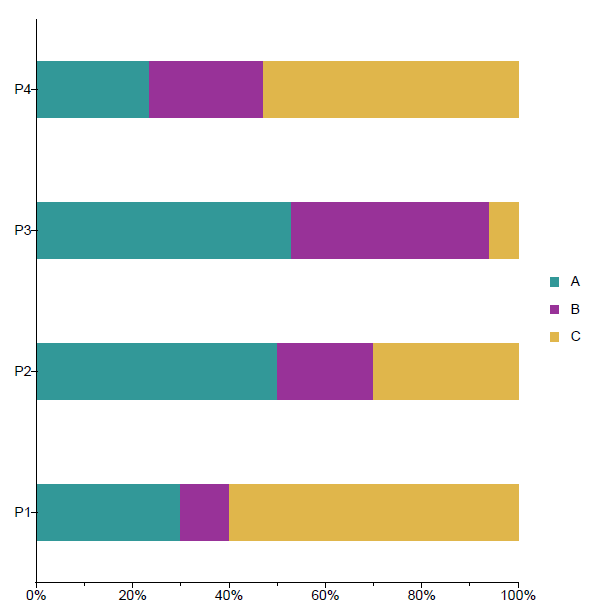
\includegraphics[scale=0.5]{figures/ch10/fig11}\caption{A stacked 100\% bar series.}\label{mar:A-stacked-100=000025}
\end{figure}

\bgroup\inputencoding{latin9}
\begin{lstlisting}[caption={A stacked 100\% indexed bar chart.},label={lis:A-stacked-100=000025},basicstyle={\small\ttfamily},breaklines=true]
using ceTe.DynamicPDF;
using ceTe.DynamicPDF.PageElements.Charting;
using ceTe.DynamicPDF.PageElements.Charting.Axes;
using ceTe.DynamicPDF.PageElements.Charting.Series;
using ceTe.DynamicPDF.PageElements.Charting.Values;
using System;

namespace ChapterExamples.Chapters.ChapterTen
{
    public class BarchartExample
    {
        public static void Create(string outputPath)
        {
            Document doc = new Document();
            doc.Pages.Add(new Page(PageSize.Letter));
            Chart chart = new Chart(0, 0, 500, 500);

            Indexed100PercentStackedBarSeries stackedBarSeries = new Indexed100PercentStackedBarSeries();
            Indexed100PercentStackedBarSeriesElement se = new Indexed100PercentStackedBarSeriesElement("A");
            se.Values.Add(new float[] { 5, 7, 9, 6 });
            Indexed100PercentStackedBarSeriesElement se2 = new Indexed100PercentStackedBarSeriesElement("B");
            se2.Values.Add(new float[] { 4, 2, 5, 8 });
            Indexed100PercentStackedBarSeriesElement se3 = new Indexed100PercentStackedBarSeriesElement("C");
            se3.Values.Add(new float[] { 2, 4, 6, 9 });

            stackedBarSeries.Add(se);
            stackedBarSeries.Add(se2);
            stackedBarSeries.Add(se3);

            chart.PrimaryPlotArea.Series.Add(stackedBarSeries);
            stackedBarSeries.YAxis.Labels.Add(new IndexedYAxisLabel("P1", 0));
            stackedBarSeries.YAxis.Labels.Add(new IndexedYAxisLabel("P2", 1));
            stackedBarSeries.YAxis.Labels.Add(new IndexedYAxisLabel("P3", 2));
            stackedBarSeries.YAxis.Labels.Add(new IndexedYAxisLabel("P4", 3));

            doc.Pages[0].Elements.Add(chart);
            doc.Draw(outputPath + "indexed-bar-stacked-100-chart-out.pdf");
        }
    }
}
\end{lstlisting}
\leavevmode\egroup


\subsection{Stacked 100\% Date/Time Data}

The \texttt{DateTime100PercentStackedBarSeries}\index{DateTime100PercentStackedBarSeries} is a collection of
\texttt{DateTime100PercentStackedBarSeriesElement}\index{DateTime100PercentStackedBarSeriesElement} instances. Each
element has a \texttt{DateTime100PercentStackedBarValueList}\index{DateTime100PercentStackedBarValueList} containing
\texttt{DateTime100PercentStackedBarValue}\index{DateTime100PercentStackedBarValue} instances. A \texttt{DateTime100PercentStackedBarSeries}\index{DateTime100PercentStackedBarSeries}
uses the \texttt{PercentageXAxis}\index{PercentageXAxis} class as the x-axis and \texttt{DateTimeYAxis}\index{DateTimeYAxis}
class as the y-axis.

Listing \ref{lis:Stacked-100=000025-data/time} illustrates creating
a 100\% stacked bar chart. You first create a \texttt{DateTime100PercentStackedBarSeries}\index{DateTime100PercentStackedBarSeries}
instance and three \texttt{DateTime100PercentStackedBarSeriesElement}\index{DateTime100PercentStackedBarSeriesElement}
instances. You then add the \texttt{DateTime100PercentStackedBarValue}\index{DateTime100PercentStackedBarValue}
instances to each element. After the elements are populated with each
element's values, you add the elements to the series. We then add
the series to the primary plot area and set the y-axis to display
the complete date of each label. Figure \ref{fig:Stackedc-100=000025-date/time}
is the resulting chart.
\begin{figure}
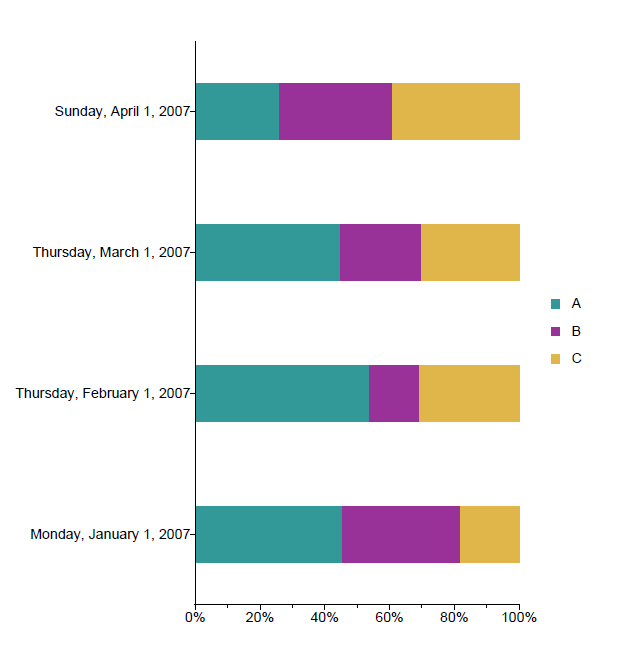
\includegraphics[scale=0.5]{figures/ch10/fig12}\caption{Stacked 100\% date/time bar chart.}\label{fig:Stackedc-100=000025-date/time}

\end{figure}
\bgroup\inputencoding{latin9}
\begin{lstlisting}[caption={Stacked 100\% data/time bar chart.},label={lis:Stacked-100=000025-data/time},basicstyle={\small\ttfamily},breaklines=true]
using ceTe.DynamicPDF;
using ceTe.DynamicPDF.PageElements.Charting;
using ceTe.DynamicPDF.PageElements.Charting.Axes;
using ceTe.DynamicPDF.PageElements.Charting.Series;
using ceTe.DynamicPDF.PageElements.Charting.Values;
using System;

namespace ChapterExamples.Chapters.ChapterTen
{
    public class BarchartExample
    {
        public static void Create(string outputPath)
        {
            Document doc = new Document();
            doc.Pages.Add(new Page(PageSize.Letter));
            Chart chart = new Chart(0, 0, 500, 500);

            DateTime100PercentStackedBarSeries stackedBarSeries = new DateTime100PercentStackedBarSeries();
            DateTime100PercentStackedBarSeriesElement se = new DateTime100PercentStackedBarSeriesElement("A");
            se.Values.Add(5, new DateTime(2007, 1, 1));
            se.Values.Add(7, new DateTime(2007, 2, 1));
            se.Values.Add(9, new DateTime(2007, 3, 1));
            se.Values.Add(6, new DateTime(2007, 4, 1));
            DateTime100PercentStackedBarSeriesElement se2 = new DateTime100PercentStackedBarSeriesElement("B");
            se2.Values.Add(4, new DateTime(2007, 1, 1));
            se2.Values.Add(2, new DateTime(2007, 2, 1));
            se2.Values.Add(5, new DateTime(2007, 3, 1));
            se2.Values.Add(8, new DateTime(2007, 4, 1));
            DateTime100PercentStackedBarSeriesElement se3 = new DateTime100PercentStackedBarSeriesElement("C");
            se3.Values.Add(2, new DateTime(2007, 1, 1));
            se3.Values.Add(4, new DateTime(2007, 2, 1));
            se3.Values.Add(6, new DateTime(2007, 3, 1));
            se3.Values.Add(9, new DateTime(2007, 4, 1));

           
            stackedBarSeries.Add(se);
            stackedBarSeries.Add(se2);
            stackedBarSeries.Add(se3);

            chart.PrimaryPlotArea.Series.Add(stackedBarSeries);

            stackedBarSeries.YAxis.LabelFormat = "D";
            doc.Pages[0].Elements.Add(chart);
            doc.Draw(outputPath + "date-time-bar-stacked-100-chart-out.pdf");
        }
    }
}
\end{lstlisting}
\leavevmode\egroup

\section{Column Chart}\label{sec:Column-Chart}

A column chart is essentially the same as a bar chart, except instead
of the bars being depicted horizontally, they are shown vertically.
A column chart can use indexed or date/time values. A column chart
can also be stacked or 100\% stacked. Table \ref{tab:column-chart-Core-Suite-classes}
lists the Core Suite classes used to create column charts. Because
creating the different column chart types is essentially the same
as creating bar charts, we only examine examples of an indexed normal
column chart and a date/time stacked column chart.
\begin{table}
\raggedright
\begin{tabular}{p{0.47\textwidth}p{0.47\textwidth}}
\toprule 
{\scriptsize Series Class} & {\scriptsize Element Class}\tabularnewline
\midrule
{\scriptsize\texttt{IndexedColumnSeries}} & {\scriptsize -}\tabularnewline
{\scriptsize\texttt{DateTimeColumnSeries}} & {\scriptsize -}\tabularnewline
{\scriptsize\texttt{IndexedStackedColumnSeries}} & {\scriptsize\texttt{IndexedStackedColumnSeriesElement}}\tabularnewline
{\scriptsize\texttt{DateTimeStackedColumnSeries}} & {\scriptsize\texttt{DateTimeStackedColumnSeriesElement}}\tabularnewline
{\scriptsize\texttt{Indexed100PercentStackedColumnSeries}} & {\scriptsize\texttt{Indexed100PercentStackedColumnSeriesElement}}\tabularnewline
{\scriptsize\texttt{DateTime100PercentStackedColumnSeries}} & {\scriptsize\texttt{DateTime100PercentStackedColumnSeriesElement}}\tabularnewline
\bottomrule
\end{tabular}\caption{Column charts.}\label{tab:column-chart-Core-Suite-classes}
\end{table}


\subsection{Normal Indexed Data}

Creating an indexed column chart is similar to creating an indexed
bar chart as Listing \ref{lis:Column-chart-with} illustrates. First,
you create three new \texttt{IndexedColumnSeries}\index{IndexedColumnSeries} instances and add
values to each instance. Next, you add the three series to the chart's
primary plot area. After adding the series, you then create the x-axis
labels. Figure \ref{mar:Column-chart-with} illustrates the resulting
chart.

\begin{figure}
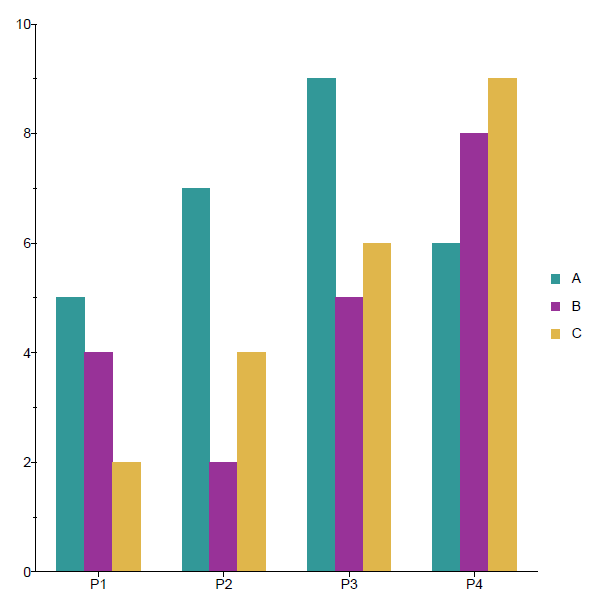
\includegraphics[scale=0.5]{figures/ch10/fig13}\caption{Column chart with indexed data.}\label{mar:Column-chart-with}
\end{figure}

\bgroup\inputencoding{latin9}
\begin{lstlisting}[caption={Column chart with indexed data.},label={lis:Column-chart-with},basicstyle={\small\ttfamily},breaklines=true]
using ceTe.DynamicPDF;
using ceTe.DynamicPDF.PageElements.Charting;
using ceTe.DynamicPDF.PageElements.Charting.Axes;
using ceTe.DynamicPDF.PageElements.Charting.Series;

namespace ChapterExamples.Chapters.ChapterTen
{
    public class ColumnChartExample
    {
        public static void Create(string outputPath)
        {
            Document doc = new Document();
            doc.Pages.Add(new Page(PageSize.Letter));
            Chart chart = new Chart(0, 0, 500, 500);

            IndexedColumnSeries cs = new IndexedColumnSeries("A");
            cs.Values.Add(new float[] { 5, 7, 9, 6 });
            IndexedColumnSeries cs2 = new IndexedColumnSeries("B");
            cs2.Values.Add(new float[] { 4, 2, 5, 8 });
            IndexedColumnSeries cs3 = new IndexedColumnSeries("C");
            cs3.Values.Add(new float[] { 2, 4, 6, 9 });
            chart.PrimaryPlotArea.Series.Add(cs);
            chart.PrimaryPlotArea.Series.Add(cs2);
            chart.PrimaryPlotArea.Series.Add(cs3);
            cs.XAxis.Labels.Add(new IndexedXAxisLabel("P1", 0));
            cs.XAxis.Labels.Add(new IndexedXAxisLabel("P2", 1));
            cs.XAxis.Labels.Add(new IndexedXAxisLabel("P3", 2));
            cs.XAxis.Labels.Add(new IndexedXAxisLabel("P4", 3));

            doc.Pages[0].Elements.Add(chart);
            doc.Draw(outputPath + "simple-column-chart-out.pdf");
        }
    }
}
\end{lstlisting}
\leavevmode\egroup


\subsection{Stacked Date/Time Data}

In Listing \ref{lis:Stacked-column-chart} you create a stacked column
chart using date/time series data. First, you create a new \texttt{DateTimeStackedColumnSeries}\index{DateTimeStackedColumnSeries}
instance. Next, you create three \texttt{DateTimeStackedColumnSeriesElement}\index{DateTimeStackedColumnSeriesElement}
instances and populate each with time series data. Next, you add the
elements to the series and the series to the chart's primary plot
area. Then you set the y-axis label format as year. Figure \ref{fig:Stacked-data/time-column}
is the resulting chart created.

\bgroup\inputencoding{latin9}
\begin{lstlisting}[caption={Stacked column chart of indexed data.},label={lis:Stacked-column-chart},basicstyle={\small\ttfamily},breaklines=true]
using ceTe.DynamicPDF.PageElements.Charting;
using ceTe.DynamicPDF.PageElements.Charting.Axes;
using ceTe.DynamicPDF.PageElements.Charting.Series;
using System;

namespace ChapterExamples.Chapters.ChapterTen
{
    public class ColumnChartExample
    {
        public static void Create(string outputPath)
        {
            Document doc = new Document();
            doc.Pages.Add(new Page(PageSize.Letter));
            Chart chart = new Chart(0, 0, 500, 500);

            DateTimeStackedColumnSeries stackedColumnSeries1 = new DateTimeStackedColumnSeries();

            DateTimeStackedColumnSeriesElement se = new DateTimeStackedColumnSeriesElement("A");
            se.Values.Add(5, new DateTime(2024, 1, 1));
            se.Values.Add(7, new DateTime(2023, 2, 1));
            se.Values.Add(9, new DateTime(2022, 3, 1));
            se.Values.Add(6, new DateTime(2021, 4, 1));

            DateTimeStackedColumnSeriesElement se2 = new DateTimeStackedColumnSeriesElement("B");
            se2.Values.Add(4, new DateTime(2024, 1, 1));
            se2.Values.Add(2, new DateTime(2023, 2, 1));
            se2.Values.Add(5, new DateTime(2022, 3, 1));
            se2.Values.Add(8, new DateTime(2021, 4, 1));

            DateTimeStackedColumnSeriesElement se3 = new DateTimeStackedColumnSeriesElement("C");
            se3.Values.Add(2, new DateTime(2024, 1, 1));
            se3.Values.Add(4, new DateTime(2023, 2, 1));
            se3.Values.Add(6, new DateTime(2022, 3, 1));
            se3.Values.Add(9, new DateTime(2021, 4, 1));

            stackedColumnSeries1.Add(se);
            stackedColumnSeries1.Add(se2);
            stackedColumnSeries1.Add(se3);

            chart.PrimaryPlotArea.Series.Add(stackedColumnSeries1);

            stackedColumnSeries1.XAxis.LabelFormat = "yyyy";

            doc.Pages[0].Elements.Add(chart);
            doc.Draw(outputPath + "column-stacked-date-chart-out.pdf");
        }
    }
}
\end{lstlisting}
\leavevmode\egroup

\begin{figure}

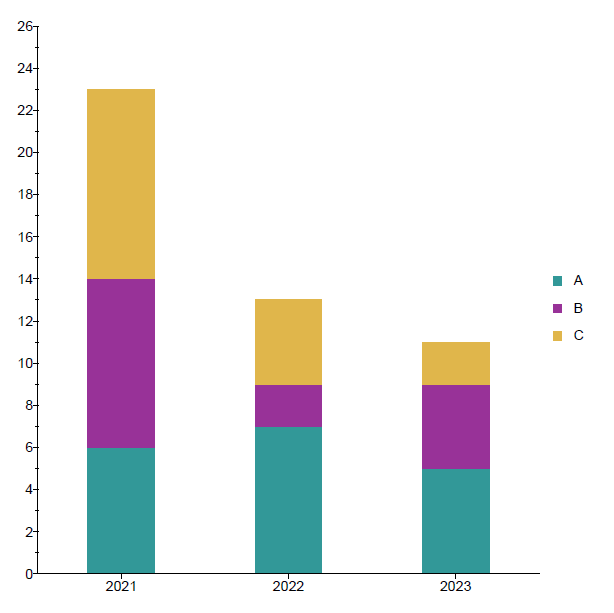
\includegraphics[scale=0.5]{figures/ch10/fig14}\caption{Stacked data/time column chart.}\label{fig:Stacked-data/time-column}

\end{figure}


\section{More on Charts}

Now that we have examined pie, bar, and column charts, before examining
the other chart's offered by Core Suite, let's revisit several other
concepts applicable to all charts.

\subsection{Property Precedence}

When creating a chart, the property precedence is as follows: $chart\rightarrow plot\,area\rightarrow series\rightarrow label$.
Properties defined by the chart are inherited by the sub-elements
of the chart. Properties defined by the plot area are inherited by
its sub-elements. For instance, you could define a font in a \texttt{Chart}\index{Chart},
legend, series, or individual data labels. When displaying the chart,
what font is used by each element would depend on either its font
or its immediate parent's font. Let's use an \texttt{IndexedBarSeries}\index{IndexedBarSeries}
example to illustrate property precedence.

In Listing \ref{lis:Property-precedence-using} you illustrate property
precedence by modifying a bar chart's font. You set the font for the
overall chart to courier bold and so any object used by the \texttt{Chart}
also uses that font. However, in the second series you change its font
to ZapfDingbats and so the value label for that font is different
then the other series, which default to the \texttt{Chart} instance's
font (courier bold). The y-axis labels also use the \texttt{Chart}
instance's font, except for the second label, which you change to ZapfDingbats.
Figure \ref{fig:Illustrating-property-precedence} illustrates the
produced chart.

\bgroup\inputencoding{latin9}
\begin{lstlisting}[caption={Property precedence using bar chart.},label={lis:Property-precedence-using},basicstyle={\small\ttfamily},breaklines=true]
using ceTe.DynamicPDF;
using ceTe.DynamicPDF.PageElements.Charting;
using ceTe.DynamicPDF.PageElements.Charting.Axes;
using ceTe.DynamicPDF.PageElements.Charting.Series;

namespace ChapterExamples.Chapters.ChapterTen
{
    public class PropertyPrecedence
    {
        public static void Create(string outputPath)
        {
            Document doc = new Document();
            doc.Pages.Add(new Page(PageSize.Letter));

            Chart chart = new Chart(0, 0, 400, 230);
            chart.Font = Font.CourierBold;
            
            chart.HeaderTitles.Add(new Title("Chart Title"));

            IndexedBarSeries barSeries = new IndexedBarSeries("A");
            barSeries.Values.Add(new float[] { 4, 5, 8, 2 });
            IndexedBarSeries barSeries2 = new IndexedBarSeries("B");
            barSeries2.Values.Add(new float[] { 1, 9, 8, 5 });
            IndexedBarSeries barSeries3 = new IndexedBarSeries("C");
            barSeries3.Values.Add(new float[] { 2, 4, 8, 3 });

            chart.PrimaryPlotArea.Series.Add(barSeries);
            chart.PrimaryPlotArea.Series.Add(barSeries2);
            chart.PrimaryPlotArea.Series.Add(barSeries3);

            barSeries2.LegendLabel.Font = Font.ZapfDingbats;
            
            barSeries.YAxis.Labels.Add(new IndexedYAxisLabel("P1", 0));
            barSeries.YAxis.Labels.Add(new IndexedYAxisLabel("P2", 1));

            barSeries.YAxis.Labels[1].Font = Font.ZapfDingbats;

            barSeries.YAxis.Labels.Add(new IndexedYAxisLabel("P3", 2));
            barSeries.YAxis.Labels.Add(new IndexedYAxisLabel("P4", 3));

            doc.Pages[0].Elements.Add(chart);
            doc.Draw(outputPath + "property-precedence-chart-out.pdf");
        }
    }
}
\end{lstlisting}
\leavevmode\egroup

\begin{figure}
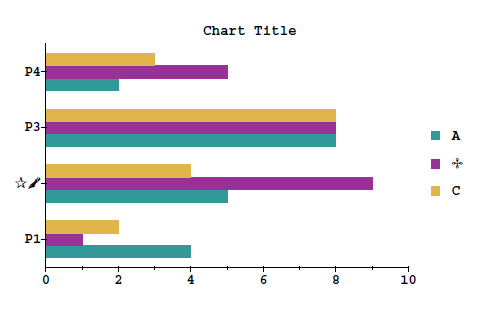
\includegraphics[scale=0.75]{figures/ch10/fig16}\caption{Illustrating property precedence when creating charts.}\label{fig:Illustrating-property-precedence}

\end{figure}


\subsection{Manual Layout}\label{sec:Manual-Layout}

So far in all our examples we have created charts using auto-layout.
However, often more fine-grained control of a chart's appearance is
required. Core Suite allows auto-layout to be overridden through the
\texttt{Chart} class's \texttt{AutoLayout} property. Set the auto-layout
property to \texttt{false} to force manual chart layout. However,
if you disable auto-layout, then when laying out a chart, you must
set the plot area's location and dimension and the legend's location
and dimension.
\noindent\begin{flushleft}
\textbf{Auto-Layout Example}
\par\end{flushleft}

Before considering manual layout, let's consider another example using
auto-layout. Listing \ref{lis:Auto-layout-example.} creates a pie
chart that uses auto-layout. The chart uses its primary plot area
and default legend and sizes the plot area and the legend automatically
(Figure \ref{mar:Auto-layout-example.}). 

If we were to then modify the code to set auto-layout to false, but
failed to specify the plot area and legend dimension and location,
we end up with the resulting chart in Figure \ref{mar:Chart-with-auto-layout}.
Not at all how we intended our chart to appear. Instead, we must manually
layout all chart elements.

\begin{figure}
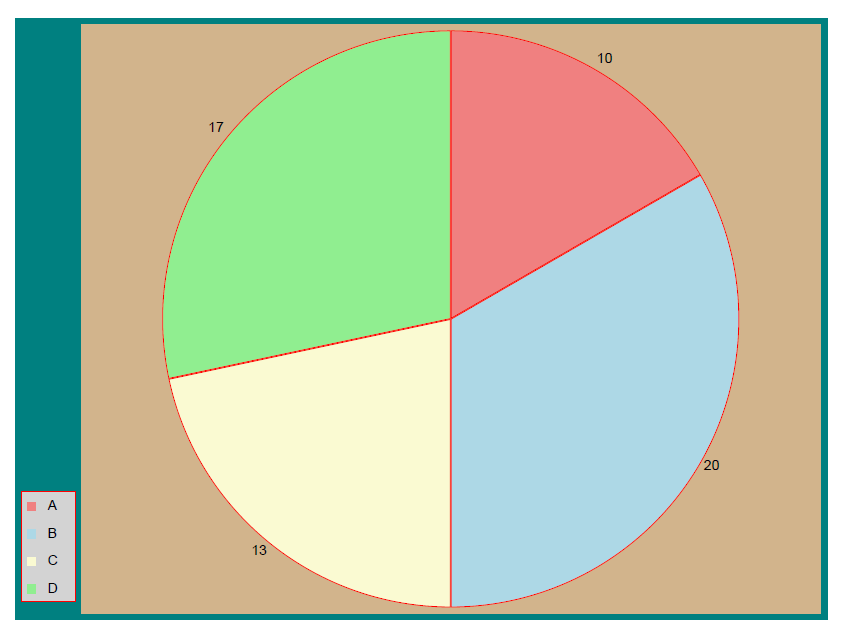
\includegraphics[scale=0.45]{figures/ch10/fig17}\caption{Auto-layout example.}\label{mar:Auto-layout-example.}

\end{figure}

\bgroup\inputencoding{latin9}
\begin{lstlisting}[caption={Auto-layout example.},label={lis:Auto-layout-example.},basicstyle={\small\ttfamily},breaklines=true]
public static void AutoLayoutExample(string outPath)
{
    Document doc = new();
    doc.Pages.Add(new Page(PageSize.Letter, PageOrientation.Landscape));

    float hght = doc.Pages[0].Dimensions.Height - doc.Pages[0].Dimensions.TopMargin * 2;
    float wdth = doc.Pages[0].Dimensions.Width - doc.Pages[0].Dimensions.RightMargin * 2;

    Chart chart = new Chart(0, 0, wdth, hght);
    chart.BackgroundColor = RgbColor.Teal;
                      
    PlotArea plotArea = chart.PrimaryPlotArea;
    plotArea.BackgroundColor = RgbColor.Tan;
   
    PieSeries pieSeries = new PieSeries();
    ScalarDataLabel dataLbl = new ScalarDataLabel(true, false, false);
    pieSeries.BorderColor = RgbColor.Red;
    pieSeries.BorderWidth = 1;
    pieSeries.DataLabel = dataLbl;
            
    plotArea.Series.Add(pieSeries);
    PieSeriesElement pe1 = new(10, "A", RgbColor.LightCoral);
    PieSeriesElement pe2 = new(20, "B", RgbColor.LightBlue);
    PieSeriesElement pe3 = new(13, "C", RgbColor.LightGoldenRodYellow);
    PieSeriesElement pe4 = new(17, "D", RgbColor.LightGreen);

    pieSeries.Elements.Add(pe1);
    pieSeries.Elements.Add(pe2);
    pieSeries.Elements.Add(pe3);
    pieSeries.Elements.Add(pe4);

    Legend legend1 = chart.Legends[0];
    legend1.BackgroundColor = RgbColor.LightGrey;
    legend1.BorderWidth = 1;
    legend1.BorderColor = RgbColor.Red;
          
    chart.Legends.Placement = LegendPlacement.BottomLeft;
    
    doc.Pages[0].Elements.Add(chart);
    doc.Draw(outPath + "autolayout-pie-chart-out.pdf");
}
\end{lstlisting}
\leavevmode\egroup

\noindent\begin{flushleft}
Because we disabled auto-layout, it placed the legend in the chart's
upper left hand corner and sized the plot area to the content needed.
However, the chart's layout was not automatic. Instead, what we must
do is modify the plot area's dimensions and the legend's dimensions,
which is what we do next.
\begin{marginfigure}
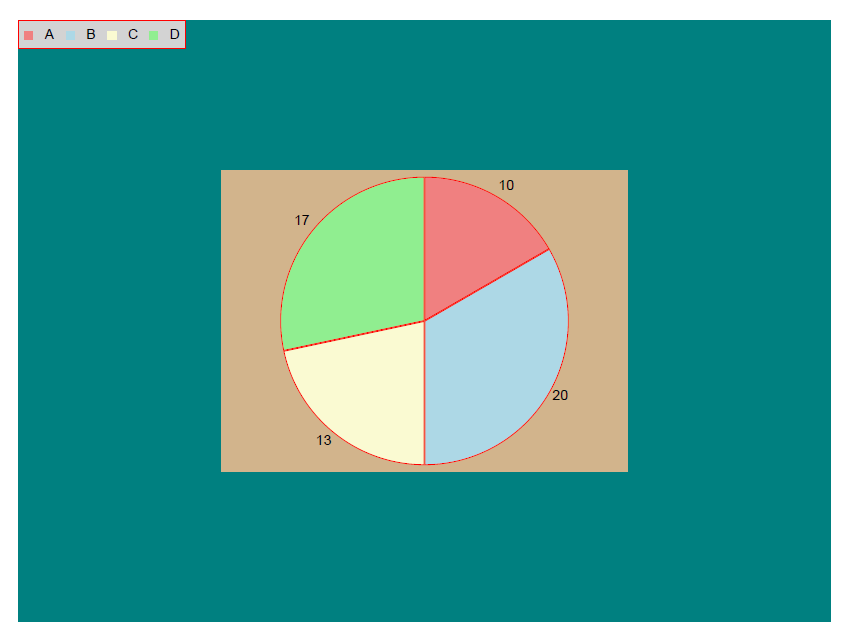
\includegraphics[scale=0.3]{figures/ch10/fig18}\caption{Chart with auto-layout disabled without formatting.}\label{mar:Chart-with-auto-layout}

\end{marginfigure}
 
\par\end{flushleft}

\noindent\begin{flushleft}
\textbf{Manual Layout Example}
\par\end{flushleft}

In Listing \ref{lis:Manually-setting-plot} you manually layout a chart
by creating a new legend rather than using the default legend. You
also remove the call to place the legend at the bottom left, as you
are manually positioning the legend. You also no longer use the primary
plot area but instead create a new plot area. The resulting chart
is illustrated in Figure \ref{fig:Manually-laying-out}.

\bgroup\inputencoding{latin9}
\begin{lstlisting}[caption={Manually setting plot area and legend.},label={lis:Manually-setting-plot},basicstyle={\small\ttfamily},breaklines=true]
using ceTe.DynamicPDF;
using ceTe.DynamicPDF.PageElements.Charting;
using ceTe.DynamicPDF.PageElements.Charting.Series;

namespace ChapterExamples.Chapters.ChapterTen
{
    public class ChartLayoutExample
    {
        public static void Create(string outputPath)
        {
            Document doc = new();
            doc.Pages.Add(new Page(PageSize.Letter, PageOrientation.Landscape));
            float hght = doc.Pages[0].Dimensions.Height - doc.Pages[0].Dimensions.TopMargin * 2;
            float wdth = doc.Pages[0].Dimensions.Width - doc.Pages[0].Dimensions.RightMargin * 2;
            
            Chart chart = new Chart(0, 0, wdth, hght);
            chart.BackgroundColor = RgbColor.Teal;
            chart.AutoLayout = false;
            
            PlotArea plotArea = chart.PlotAreas.Add(100, 100, wdth / 2, hght * .75F);
            plotArea.BackgroundColor = RgbColor.Tan;
            Legend legend1 = chart.Legends.Add(470, 250, 40, 100);
            legend1.BackgroundColor = RgbColor.LightGrey;
            legend1.BorderWidth = 1;
            legend1.BorderColor = RgbColor.Red;

            PieSeries pieSeries = new PieSeries(legend1);
            ScalarDataLabel dataLbl = new ScalarDataLabel(true, false, false);
            pieSeries.BorderColor = RgbColor.Red;
            pieSeries.BorderWidth = 1;
            pieSeries.DataLabel = dataLbl;
            plotArea.Series.Add(pieSeries);

            PieSeriesElement pe1 = new(10, "A ", RgbColor.LightCoral);
            PieSeriesElement pe2 = new(20, "B ", RgbColor.LightBlue);
            PieSeriesElement pe3 = new(13, "C ", RgbColor.LightGoldenRodYellow);
            PieSeriesElement pe4 = new(17, "D ", RgbColor.LightGreen);
            pieSeries.Elements.Add(pe1);
            pieSeries.Elements.Add(pe2);
            pieSeries.Elements.Add(pe3);
            pieSeries.Elements.Add(pe4);

            doc.Pages[0].Elements.Add(chart);
            doc.Draw(outputPath + "manual-layout-pie-chart-out.pdf");
        }
    }
}
\end{lstlisting}
\leavevmode\egroup

\begin{figure}
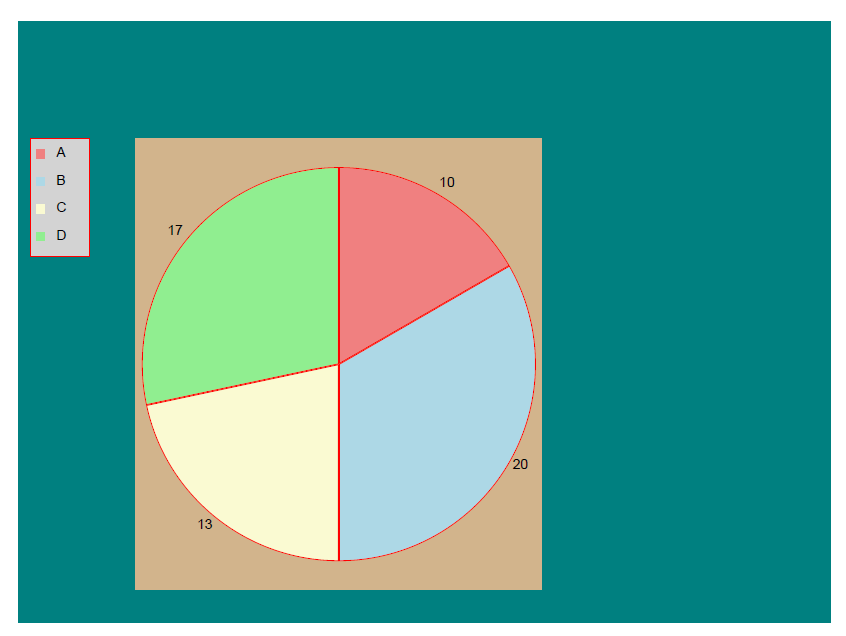
\includegraphics[scale=0.5]{figures/ch10/fig19}\caption{Manually laying out a pie chart.}\label{fig:Manually-laying-out}
\end{figure}

Notice the chart in Figure \ref{fig:Manually-laying-out} now respects
the settings made for its plot area location and boundaries. It also
respects the legend's settings. It positioned the plot area at (100,100)
and the width and height as 1/2 the page's width and 3/4 the page's
height (accounting for the page's margins). It also positioned the
legend at (470, 250) and set its width to 40 and height to 100.
\noindent\begin{flushleft}
\textbf{Modifying Layout Manually}
\par\end{flushleft}

Manually calculating the layout for all a \texttt{Chart} instance's
elements can be error-prone and time-consuming. Moreover, you might
only wish to modify a few aspects of a chart's layout. Core Suite
provides a \texttt{Layout} method for the \texttt{Chart} class to
handle these situations. What you do is create the chart and its elements
as you would normally. After adding all the chart's elements, disable
auto-layout and call the \texttt{Layout} method. When \texttt{Layout}
is called, it automatically calculates the \texttt{Chart} instance's
layout (as if you had set auto-layout to true). Then, after the \texttt{Layout}
method call, you can modify the different \texttt{Chart} elements
manually.

Listing \ref{lis:Modifying-a-chart's} illustrates modifying a chart's
layout. You first add the data series to the primary plot area. Notice
Listing \ref{lis:Modifying-a-chart's} relies upon the primary plot
area and the default legend; so no formatting of either is required.
\begin{figure}
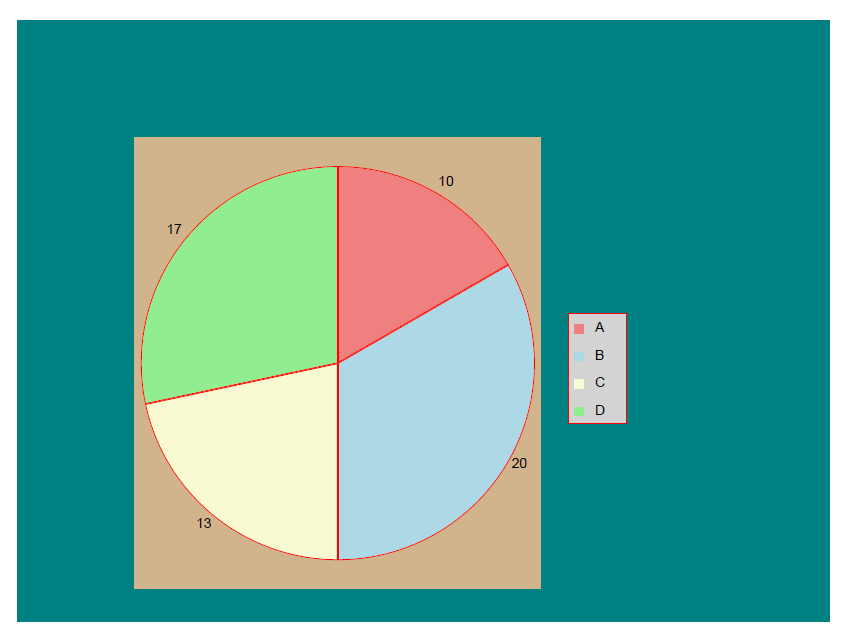
\includegraphics[scale=0.5]{figures/ch10/fig21}\caption{Modifying a chart's layout manually.}\label{fig:Modifying-a-chart's}
\end{figure}
 

In Listing \ref{lis:Modifying-a-chart's} you then disable auto-layout
and call the \texttt{Layout} method. This automatically determines
the chart's layout by calling this method. After determining the chart's
layout, you then modify the plot's location and dimensions and the
legend's location. Note that you do not modify the legend's dimensions,
those remain unchanged from what is calculated by the \texttt{Layout}
method. Figure \ref{fig:Modifying-a-chart's} illustrates the resulting
chart.

\bgroup\inputencoding{latin9}
\begin{lstlisting}[caption={Modifying a chart's layout manually.},label={lis:Modifying-a-chart's},basicstyle={\small\ttfamily},breaklines=true]
using ceTe.DynamicPDF;
using ceTe.DynamicPDF.PageElements.Charting;
using ceTe.DynamicPDF.PageElements.Charting.Series;

namespace ChapterExamples.Chapters.ChapterTen
{
    public class ChartLayoutExample
    {
        public static void Create(string outputPath)
        {
            Document doc = new();
            doc.Pages.Add(new Page(PageSize.Letter, PageOrientation.Landscape));
            float hght = doc.Pages[0].Dimensions.Height - doc.Pages[0].Dimensions.TopMargin * 2;
            float wdth = doc.Pages[0].Dimensions.Width - doc.Pages[0].Dimensions.RightMargin * 2;

            Chart chart = new Chart(0, 0, wdth, hght);
            chart.BackgroundColor = RgbColor.Teal;
            chart.PrimaryPlotArea.BackgroundColor = RgbColor.Tan;

            PieSeries pieSeries = new PieSeries();
            ScalarDataLabel dataLbl = new ScalarDataLabel(true, false, false);
            pieSeries.BorderColor = RgbColor.Red;
            pieSeries.BorderWidth = 1;
            pieSeries.DataLabel = dataLbl;
            chart.PrimaryPlotArea.Series.Add(pieSeries);

            PieSeriesElement pe1 = new(10, "A ", RgbColor.LightCoral);
            PieSeriesElement pe2 = new(20, "B ", RgbColor.LightBlue);
            PieSeriesElement pe3 = new(13, "C ", RgbColor.LightGoldenRodYellow);
            PieSeriesElement pe4 = new(17, "D ", RgbColor.LightGreen);
            pieSeries.Elements.Add(pe1);
            pieSeries.Elements.Add(pe2);
            pieSeries.Elements.Add(pe3);
            pieSeries.Elements.Add(pe4);

            chart.Legends[0].BackgroundColor = RgbColor.LightGrey;
            chart.Legends[0].BorderWidth = 1;
            chart.Legends[0].BorderColor = RgbColor.Red;
            
            chart.AutoLayout = false;
            chart.Layout();
            
            chart.PrimaryPlotArea.X = 100;
            chart.PrimaryPlotArea.Y = 100;
            chart.PrimaryPlotArea.Width = wdth / 2;
            chart.PrimaryPlotArea.Height = hght * .75F;
            chart.Legends[0].X = 470;
            chart.Legends[0].Y = 250;

            doc.Pages[0].Elements.Add(chart);
            doc.Draw(outputPath + "modify-layout-pie-chart-out.pdf");
        }
    }
}
\end{lstlisting}
\leavevmode\egroup

\noindent\begin{flushleft}
\textbf{Multiple Plot Areas}
\par\end{flushleft}

A chart can have multiple plot areas. Let's revisit adding plot areas
to a chart by adding a plot area containing a pie series and a plot
area containing a bar series to the same chart. When adding multiple
plot areas to the same chart, it's best to disable auto-layout, as
auto-layout places the plot areas too closely together and does not
allow fine-grained layout of your plot areas.\sidenote{If you add titles to the plot areas, then Core Suite adds spacing
between plot areas.}

When adding multiple plot areas, you usually want to create multiple
legends, each with its own data series. Each legend is associated
with the relevant data from the series in the different plot areas.
For example, in Listing \ref{lis:two-plot-A-chart-with} we create
a chart with two plot areas, one containing a pie series and the other
a bar series. 

First, you create a new \texttt{Chart} instance and initializes its
dimensions to the page's dimensions (minus accounting for the margins).
Next you create two legends, also initializing the location and dimension
of both. After creating the legends, you create the pie series and
assign the first legend to the pie series. You then create a plot area
and add the series to the plot area. 

After creating the pie series, you create a bar series. You assign
the second legend to the bar series, create a plot area, and add the
bar series to the second plot area. We then add the bar series y-axis
labels.

After adding both series to their respective plot areas, you set the
\texttt{Chart} instance's \texttt{AutoLayout} property to false and
adds the \texttt{Chart} instance to the page. Note that you do not
call the instance's \texttt{Layout} method, as that would invalidate
the manual locations and dimensions of the plot areas and legends.
Figure \ref{fig:two-plot-A-chart-with} illustrates the resulting
PDF document.
\begin{figure}[h]
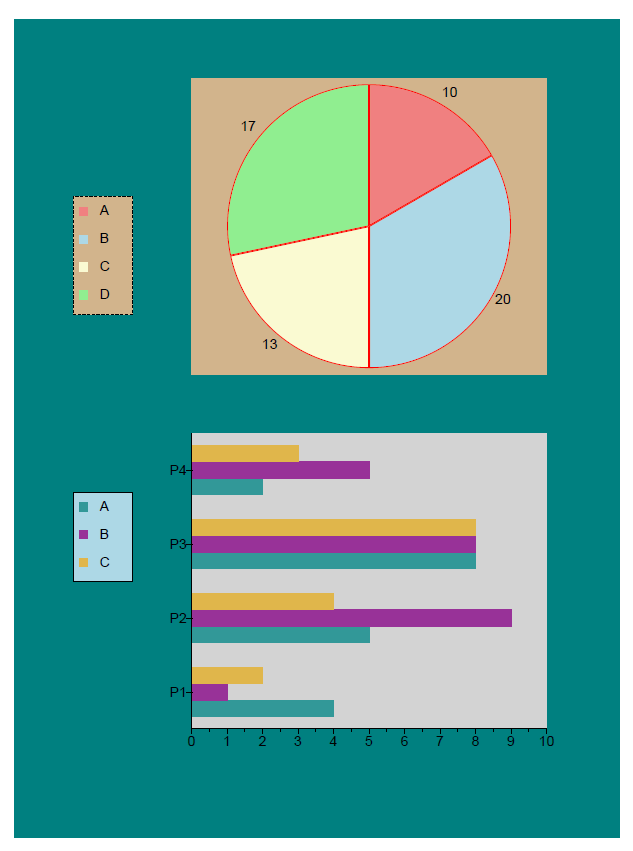
\includegraphics[scale=0.65]{figures/ch10/fig20}\caption{A chart with two plot areas.}\label{fig:two-plot-A-chart-with}
\end{figure}

\bgroup\inputencoding{latin9}
\begin{lstlisting}[caption={A chart with two plot areas.},label={lis:two-plot-A-chart-with},basicstyle={\small\ttfamily},breaklines=true]
using ceTe.DynamicPDF;
using ceTe.DynamicPDF.PageElements.Charting;
using ceTe.DynamicPDF.PageElements.Charting.Axes;
using ceTe.DynamicPDF.PageElements.Charting.Series;

namespace ChapterExamples.Chapters.ChapterTen
{
    public class MultiplePlotAreas
    {

        public static void Create(string outputPath)
        {
            Document doc = new Document();
            doc.Pages.Add(new Page(PageSize.Letter));

            float hght = doc.Pages[0].Dimensions.Height - doc.Pages[0].Dimensions.TopMargin * 2;
            float wdth = doc.Pages[0].Dimensions.Width - doc.Pages[0].Dimensions.RightMargin * 2;

            Chart chart = new Chart(0, 0, wdth, hght);
            chart.BackgroundColor = RgbColor.Teal;

            Legend legend = chart.Legends.Add(50, 150, 50, 100);
            legend.BorderColor = RgbColor.Black;
            legend.BackgroundColor = RgbColor.Tan;
            legend.BorderStyle = LineStyle.DashSmall;

            Legend legend2 = chart.Legends.Add(40, 400, 50, 75);
            legend2.BackgroundColor = RgbColor.LightBlue;
            legend2.BorderColor = RgbColor.Black;
            legend2.BorderStyle = LineStyle.Solid;

            PlotArea plotArea = chart.PlotAreas.Add(150, 50, 300, 250);
            plotArea.BackgroundColor = RgbColor.Tan;


            PieSeries pieSeries = new PieSeries();
            ScalarDataLabel dataLbl = new ScalarDataLabel(true, false, false);
            pieSeries.BorderColor = RgbColor.Red;
            pieSeries.BorderWidth = 1;
            pieSeries.DataLabel = dataLbl;


            plotArea.Series.Add(pieSeries);

            PieSeriesElement pe1 = new(10, "A", RgbColor.LightCoral);
            PieSeriesElement pe2 = new(20, "B", RgbColor.LightBlue);
            PieSeriesElement pe3 = new(13, "C", RgbColor.LightGoldenRodYellow);
            PieSeriesElement pe4 = new(17, "D", RgbColor.LightGreen);
            pe1.Legend = legend;

            pieSeries.Elements.Add(pe1);
            pieSeries.Elements.Add(pe2);
            pieSeries.Elements.Add(pe3);
            pieSeries.Elements.Add(pe4);


            PlotArea plotArea2 = chart.PlotAreas.Add(150, 350, 300, 250);
            plotArea2.BackgroundColor = RgbColor.LightGrey;

            IndexedBarSeries barSeries = new IndexedBarSeries("A");
            barSeries.Values.Add(new float[] { 4, 5, 8, 2 });
            barSeries.Legend = legend2;
            IndexedBarSeries barSeries2 = new IndexedBarSeries("B");
            barSeries2.Legend = legend2;
            barSeries2.Values.Add(new float[] { 1, 9, 8, 5 });
            IndexedBarSeries barSeries3 = new IndexedBarSeries("C");
            barSeries3.Legend = legend2;
            barSeries3.Values.Add(new float[] { 2, 4, 8, 3 });

            plotArea2.Series.Add(barSeries);
            plotArea2.Series.Add(barSeries2);
            plotArea2.Series.Add(barSeries3);

            barSeries.YAxis.Labels.Add(new IndexedYAxisLabel("P1", 0));
            barSeries.YAxis.Labels.Add(new IndexedYAxisLabel("P2", 1));
            barSeries.YAxis.Labels.Add(new IndexedYAxisLabel("P3", 2));
            barSeries.YAxis.Labels.Add(new IndexedYAxisLabel("P4", 3));

            chart.AutoLayout = false;


            doc.Pages[0].Elements.Add(chart);
            doc.Draw(outputPath + "multiplot-manual-chart-out.pdf");

        }
    }
}
\end{lstlisting}
\leavevmode\egroup

\section{AutoLayout}
\label{section:autolayout-charts}
You can use the \texttt{AutoLayout}\index{AutoLayout} class to add charts automatically to a \texttt{Document} instance just as you can other page elements (see Chapter \ref{sec:autolayout}, \ref{section:autolayout-shape}, \ref{section:autolayout-image}, and \ref{section:autolayout-table}). The following example illustrates (Listing \ref{lis:autolayout-chart}).

\bgroup\inputencoding{latin9}
\begin{lstlisting}[caption={Using AutoLayout to create a PDF document.},label={lis:autolayout-chart},basicstyle={\small\ttfamily},breaklines=true]
using ceTe.DynamicPDF;
using ceTe.DynamicPDF.PageElements;
using ceTe.DynamicPDF.PageElements.Charting;
using ceTe.DynamicPDF.PageElements.Charting.Series;

namespace ChapterExamples.Chapters.ChapterTen
{
    public class AutoLayoutExampleChart
    {
        public static void Create(string outputPath)
        {
            AutoLayout autoLayout = new AutoLayout(PageSize.Letter, PageOrientation.Portrait, 50);
            
            Chart chart = autoLayout.AddChart(300, 350);
            PieSeries pieSeries = new PieSeries();
            ScalarDataLabel dataLabel = new ScalarDataLabel(true, false, false);
            pieSeries.DataLabel = dataLabel;
            PieSeriesElement pe1 = new(10, "A", RgbColor.Navy);
            PieSeriesElement pe2 = new(20, "B", RgbColor.Red);
            pieSeries.Elements.Add(pe1);
            pieSeries.Elements.Add(pe2);
            chart.PrimaryPlotArea.Series.Add(pieSeries);

            Document document = autoLayout.GetDocument();
            document.Draw(outputPath);

        }
    }
}
\end{lstlisting}
\leavevmode\egroup


\section{Summary}

In this chapter, we covered a lot of ground. First, you learned about
the common elements of all charts. When creating a chart, you make
a Chart instance and add one or more plot areas. A plot area is a
section of the chart where data is plotted. Each plot area has one
or more data series. A data series is a set of related data points.
The type of data series determines the type of chart created. 

You can customize a chart's appearance and layout when creating a
chart. Every Chart has a primary plot area by default if you do not
wish to create a plot area. Every Chart also has a default legend.
However, you can override these defaults and create plot areas and
legends. Moreover, you can customize their appearance, position, and
dimensions. 

You learned how to create pie, bar, and column charts and how to use
indexed and date/time data. For bar and column charts, we saw that
you can build both stacked and 100\% stacked versions of the two types
of charts.

In the next chapter, we'll delve even deeper into charting. We'll
examine not only the x-axis and y-axis and how to customize both but
also cover line and scatter charts. You will learn how to add grid
lines to your charts and how to customize data markers and tick marks.
By the end of the next chapter, you'll understand the steps and customization
options available when creating a chart using DynamicPDF Core
Suite for .NET.

\color{white}
\chapter{Charts II}\label{chap:Charts-II}
\color{black}
\BgThispage
\vspace{8.00em}
\lettrine[lines=2,lhang=0.1]{I}{n} the previous chapter, you learned how to create pie, bar, and column charts, as well as how to work with plot areas, legends, and multiple plot areas. This chapter builds on that foundation by introducing line, area, and scatter charts. Additionally, we explore how to customize the x and y axes, add symbols, tick marks, and grid lines, incorporate markers, and modify data labels.

\section{Line Chart}\label{sec:Line-Chart}

A line chart displays information as a series of data points connected
by straight-line segments. Line charts can also visualize date/time
data (a time series) drawn chronologically. DynamicPDF Core Suite
for .NET provides six types of line charts: normal indexed, date/time,
stacked indexed, stacked date/time, 100\% stacked indexed, and 100\%
stacked date/time. Table \ref{tab:line-chart-Core-Suite-classes-1-1}
lists the classes offered by Core Suite for creating line charts.

\begin{table}
\raggedright
\begin{tabular}{p{0.45\textwidth}p{0.5\textwidth}}
\toprule 
{\scriptsize Series Class} & {\scriptsize Element Class}\tabularnewline
\midrule
{\scriptsize\texttt{IndexedLineSeries}} & {\scriptsize\texttt{-}}\tabularnewline
{\scriptsize\texttt{DateTimeLineSeries}} & {\scriptsize\texttt{-}}\tabularnewline
{\scriptsize\texttt{IndexedStackedLineSeries}} & {\scriptsize\texttt{IndexedStackedLineSeriesElement}}\tabularnewline
{\scriptsize\texttt{DateTimeStackedLineSeries}} & {\scriptsize\texttt{DateTimeStackedLineSeriesElement}}\tabularnewline
{\scriptsize\texttt{Indexed100PercentStackedLineSeries}} & {\scriptsize\texttt{Indexed100PercentStackedLineSeriesElement}}\tabularnewline
{\scriptsize\texttt{DateTime100PercentStackedLineSeries}} & {\scriptsize\texttt{DateTime100PercentStackedLineSeriesElement}}\tabularnewline
\bottomrule
\end{tabular}\caption{Line chart classes.}\label{tab:line-chart-Core-Suite-classes-1-1}
\end{table}
\medskip{}
The class names in Table \ref{tab:line-chart-Core-Suite-classes-1-1}
should appear familiar, similar to the bar and column chart classes
in the previous chapter. The indexed and date/time series add data
directly to the series using its \texttt{Add} method. In contrast,
like the bar and column charts in the previous chapter, the stacked
and 100\% stacked series add values to its associated elements rather
than directly to the series. 

In the following six sections, we provide examples of each line series.
Let's start by examining a normal indexed line chart.

\subsection{Normal Indexed Data}

Normal indexed line charts create lines based on indexed data using
the \texttt{IndexedLineSeries}\index{IndexedLineSeries} class. This series uses \texttt{IndexedXAxis}\index{IndexedXAxis}
instances for the x-axis labels and \texttt{NumericYAxis}\index{NumericYAxis} instances
for the y-axis labels. An indexed line series uses a data array to
represent the series values. The position in the array determines
the x-axis value, while the position’s value determines its y-axis
label. 

In Listing \ref{lis:Line-indx-chart-using} you create a line chart
using indexed data. You first create three \texttt{IndexedLineSeries}\index{IndexedLineSeries}
instances and provide data to the series using its Values property.
The Values property is an \texttt{IndexedLineValueList}\index{IndexedLineValueList} instance that
has an \texttt{Add} method for adding the actual values. After adding
the values, you then add the x-axis labels. Each x-axis label corresponds
with the value in the values for the series. For example, the first
series has an array of values: 48, 83, 19, and 23. The x-axis labels
correspond with the 0, 1, 2, and 3 array positions. The same is true
for the second series. After creating the series, you add titles for
the x and y axes and add the chart to the page. Figure \ref{mar:Line-indx-chart-using}
illustrates the resulting line chart.

\bgroup\inputencoding{latin9}
\begin{lstlisting}[caption={Line chart using indexed data.},label={lis:Line-indx-chart-using},basicstyle={\small\ttfamily},breaklines=true]
using ceTe.DynamicPDF;
using ceTe.DynamicPDF.PageElements.Charting;
using ceTe.DynamicPDF.PageElements.Charting.Axes;
using ceTe.DynamicPDF.PageElements.Charting.Series;
using System;

namespace ChapterExamples.Chapters.ChapterEleven
{
    public class LineChartExample
    {
        public static void Create(string outputPath)
        {
            Document doc = new();
            doc.Pages.Add(new Page(PageSize.Letter));

            float hght = doc.Pages[0].Dimensions.Height - doc.Pages[0].Dimensions.TopMargin * 2;
            float wdth = doc.Pages[0].Dimensions.Width - doc.Pages[0].Dimensions.RightMargin * 2;

            Chart chart = new Chart(0, 0, wdth, hght);

            IndexedLineSeries ls = new IndexedLineSeries("A");
            ls.Values.Add(new float[] { 48, 83, 19, 23 });
            IndexedLineSeries ls2 = new IndexedLineSeries("B");
            ls2.Values.Add(new float[] { 52, 74, 9, 21 });
            IndexedLineSeries ls3 = new IndexedLineSeries("C");
            ls3.Values.Add(new float[] { 15, 43, 12, 8 });
                        
            chart.PrimaryPlotArea.Series.Add(ls);
            chart.PrimaryPlotArea.Series.Add(ls2);
            chart.PrimaryPlotArea.Series.Add(ls3);

            
            ls.XAxis.Labels.Add(new IndexedXAxisLabel("NW", 0));
            ls.XAxis.Labels.Add(new IndexedXAxisLabel("SW", 1));
            ls.XAxis.Labels.Add(new IndexedXAxisLabel("SE", 2));
            ls.XAxis.Labels.Add(new IndexedXAxisLabel("NE", 3));

      ls.YAxis.Titles.Add(new Title("Items"));
            ls.XAxis.Titles.Add(new Title("Region"));

            doc.Pages[0].Elements.Add(chart);

            doc.Draw(outputPath + "line-chart-indexed-out.pdf");
        }
    }
}
\end{lstlisting}
\leavevmode\egroup

\begin{figure}[h]

\includegraphics[scale=0.5]{figures/ch11/fig1}\caption{Line chart using indexed data.}\label{mar:Line-indx-chart-using}
\end{figure}

As Figure \ref{mar:Line-indx-chart-using} shows, the y-axis title
displays the item count while the x-axis title displays the region.
The legend displays the three series names: A, B, and C. Each segment
displays the region/value combination. For example, the SW region
has 83 items for item A, 74 items for item B, and 43 for item C.

\subsection{Normal Date/Time Data}

Line charts can also display date/time series data using the \texttt{DateTimeLineSeries}\index{DateTimeLineSeries}
class. Like the normal indexed line series, this series adds values
directly to its \texttt{Values} property. The \texttt{Values} property
is a \texttt{DateTimeLineValueList}\index{DateTimeLineValueList} instance that contains one or
more \texttt{DateTimeLineValue}\index{DateTimeLineValue} instances. The value instance consists
of a numeric value and a date. The y-axis plots the numeric values
while the x-axis plots the date/time values.

Listing \ref{lis:Line-dt-chart-using} illustrates creating a line
chart with date/time data. First you create two \texttt{DateTimeLineSeries}\index{DateTimeLineSeries}
instances and add \texttt{DateTimeLineValue}\index{DateTimeLineValue} instance to each series's
\texttt{DateTimeLineValueList}\index{DateTimeLineValueList}. After adding the values, you add the
two series to the plot area. Next you assign titles for the x and y
axes and assign the date/time format for the x-axis labels. The y-axis
values are the numeric values from each \texttt{DateTimeLineValue}\index{DateTimeLineValue}
instance while the x-axis values are the corresponding date/time values.
After creating the series, you add the series to the plot area followed
by the \texttt{Chart} instance to the page. Figure \ref{fig:Line-dt-chart-using}
illustrates the resulting chart. 

\bgroup\inputencoding{latin9}
\begin{lstlisting}[caption={Line chart using date/time data.},label={lis:Line-dt-chart-using},basicstyle={\small\ttfamily},breaklines=true]
using ceTe.DynamicPDF;
using ceTe.DynamicPDF.PageElements.Charting;
using ceTe.DynamicPDF.PageElements.Charting.Axes;
using ceTe.DynamicPDF.PageElements.Charting.Series;

namespace ChapterExamples.Chapters.ChapterEleven
{
    public class LineChartExample
    {
        public static void Create(string outputPath)
        {
            Document doc = new();
            doc.Pages.Add(new Page(PageSize.Letter, PageOrientation.Landscape));

            float hght = doc.Pages[0].Dimensions.Height - doc.Pages[0].Dimensions.TopMargin * 2;
            float wdth = doc.Pages[0].Dimensions.Width - doc.Pages[0].Dimensions.RightMargin * 2;

            Chart chart = new Chart(0, 0, wdth, hght);

            DateTimeLineSeries ls = new DateTimeLineSeries("A");

            ls.Values.Add(5, new DateTime(2007, 1, 1));
            ls.Values.Add(7, new DateTime(2007, 2, 1));
            ls.Values.Add(9, new DateTime(2007, 3, 1));
            ls.Values.Add(6, new DateTime(2007, 4, 1));
            DateTimeLineSeries ls2 = new DateTimeLineSeries("B");
            ls2.Values.Add(4, new DateTime(2007, 1, 1));
            ls2.Values.Add(2, new DateTime(2007, 2, 1));
            ls2.Values.Add(5, new DateTime(2007, 3, 1));
            ls2.Values.Add(8, new DateTime(2007, 4, 1));
           
            chart.PrimaryPlotArea.Series.Add(ls);
            chart.PrimaryPlotArea.Series.Add(ls2);

            ls.YAxis.Titles.Add(new Title("Items Purchases"));

            ls.XAxis.LabelFormat = "MM/dd/yy";
            ls.XAxis.Titles.Add(new Title("Sales Date"));

            doc.Pages[0].Elements.Add(chart);
            doc.Draw(outputPath + "line-chart-datetime-out.pdf");
        }
    }
}
\end{lstlisting}
\leavevmode\egroup

\begin{figure}

\includegraphics[scale=0.5]{figures/ch11/fig2}\caption{Line chart using date/time data.}\label{fig:Line-dt-chart-using}
\end{figure}

As Figure \ref{fig:Line-dt-chart-using} illustrates, the chart shows
the date/time value compared to the items purchased for Items A and
B. For instance, on 02/01/07 Item A sold seven items while B sold
two. The chart's segments for each series was drawn between each set
of data points. The x-axis shows the dates, while the y-axis shows
the numeric values.

\subsection{Indexed Stacked}

Like a stacked bar chart, a stacked line chart displays its series
values one on top of the other and represents and compares segments
of a whole. Each line is a different data series, and each value is
a particular category. Core Suite supports creating stacked indexed
line charts with the \texttt{IndexedStackedLineSeries}\index{IndexedStackedLineSeries} class. To create
a stacked indexed line chart, you must first create an \texttt{IndexedStackedLineSeries}\index{IndexedStackedLineSeries}
instance. An \texttt{IndexedStackedLineSeries}\index{IndexedStackedLineSeries} instance contains one
or more \texttt{IndexedStackedLineSeriesElement}\index{IndexedStackedLineSeriesElement} instances. An element
instance contains one or more \texttt{IndexedStackLineValue}\index{IndexedStackLineValue} instances.
An \texttt{IndexedStackedLineValue}\index{IndexedStackedLineValue} consists of a value and position. 

Listing \ref{lis:Stacked-indexed-line-chart} illustrates creating
a stacked indexed line chart. First, you create an \texttt{IndexedStackedLineSeries}\index{IndexedStackedLineSeries}
instance and two \texttt{IndexedStackedLineSeriesElement}\index{IndexedStackedLineSeriesElement} instances.
Then, you add values to each element. Note that the values added are
an array of numeric values rather then specifically creating a value
with a numeric value and a position. In this situation, each value
is the value in the array value while the array position is the \texttt{IndexedStackLineValue}\index{IndexedStackLineValue}
instance's position. 

After creating the elements, you add the elements to the series and
the series to the plot area. You then add x-axis labels and titles
to the x and y axes. Figure \ref{mar:Stacked-indexed-line} illustrates
the resulting chart.

\bgroup\inputencoding{latin9}
\begin{lstlisting}[caption={Stacked indexed line chart.},label={lis:Stacked-indexed-line-chart},basicstyle={\small\ttfamily},breaklines=true]
using ceTe.DynamicPDF;
using ceTe.DynamicPDF.PageElements.Charting;
using ceTe.DynamicPDF.PageElements.Charting.Axes;
using ceTe.DynamicPDF.PageElements.Charting.Series;

namespace ChapterExamples.Chapters.ChapterEleven
{
    public class LineChartExample
    {
        public static void Create(string outputPath)
        {
            Document doc = new();
            doc.Pages.Add(new Page(PageSize.Letter, PageOrientation.Landscape));

            float hght = doc.Pages[0].Dimensions.Height - doc.Pages[0].Dimensions.TopMargin * 2;
            float wdth = doc.Pages[0].Dimensions.Width - doc.Pages[0].Dimensions.RightMargin * 2;

            Chart chart = new Chart(0, 0, wdth, hght);

            IndexedStackedLineSeries ls = new IndexedStackedLineSeries();
            IndexedStackedLineSeriesElement se = new IndexedStackedLineSeriesElement("A");
            se.Values.Add(new float[] { 32, 17, 19, 6 });
            IndexedStackedLineSeriesElement se2 = new IndexedStackedLineSeriesElement("B");
            se2.Values.Add(new float[] { 24, 42, 5, 18 });

            ls.Add(se);
            ls.Add(se2);
          
            chart.PrimaryPlotArea.Series.Add(ls);

            ls.XAxis.Labels.Add(new IndexedXAxisLabel("NW", 0));
            ls.XAxis.Labels.Add(new IndexedXAxisLabel("SW", 1));
            ls.XAxis.Labels.Add(new IndexedXAxisLabel("SE", 2));
            ls.XAxis.Labels.Add(new IndexedXAxisLabel("NE", 3));
            ls.YAxis.Titles.Add(new Title("Item Purchased"));
            ls.XAxis.Titles.Add(new Title("Region"));
            doc.Pages[0].Elements.Add(chart);
            doc.Draw(outputPath + "line-chart-indexed-stacked-out.pdf");
        }
    }
}
\end{lstlisting}
\leavevmode\egroup

\begin{figure}[h]

\includegraphics[scale=0.55]{figures/ch11/fig3}\caption{Stacked indexed line chart.}\label{mar:Stacked-indexed-line}
\end{figure}

On first glance, Figure \ref{mar:Stacked-indexed-line} appears similar
to Figure \ref{mar:Line-indx-chart-using}. However, if you review
the y-axis, you see that the values are stacked. For example, the
NW region sold 32 type A items and 24 type B items. The type A item’s
value is displayed at 32 on the y-axis, while the B item’s value is
displayed at 56 rather than 32, stacking the values for the NW region.
The other regions are similarly stacked.

\subsection{Date/Time Stacked}

A stacked date/time line chart also stacks its lines but it uses date/-time
data rather than indexed data. The \texttt{DateTimeStackedLineSeries}\index{DateTimeStackedLineSeries}
class represents a stacked date/timeline series. Like the stacked
series you have seen previously, this class uses one or more \texttt{DateTimeStackedLineSeriesElement}\index{DateTimeStackedLineSeriesElement}
instances that are added to a series. Element instances have a \texttt{DateTimeStackedLineValueList}\index{DateTimeStackedLineValueList}
that contains one or more \texttt{DateTimeStackedLineValue}\index{DateTimeStackedLineValue} instances.
The value instances consist of the data value and the date. You build
the series by adding values to an element's \texttt{Values} list and
then adding the element to the series's \texttt{Values} list.

In Listing \ref{lis:Stacked-date/time-line} you create a stacked date/time
line chart. First, you add a \texttt{DateTimeStackedLineSeries}\index{DateTimeStackedLineSeries} instance
and two \texttt{DateTimeStackedLineSeriesElement}\index{DateTimeStackedLineSeriesElement} instances. Each
element adds \texttt{DateTimeStackedLineValue}\index{DateTimeStackedLineValue} instances to its \texttt{DateTimeStackedLineValueList}\index{DateTimeStackedLineValueList}.
After creating the elements, you add the elements to the series and
the series to the plot area. You then create titles for the x and y
axes and set the x-axis date/time format. Figure \ref{fig:Stacked-date/time-line}
illustrates the resulting chart.
\begin{figure}

\includegraphics[scale=0.5]{figures/ch11/fig4}\caption{Stacked date/time line chart.}\label{fig:Stacked-date/time-line}
\end{figure}

\bgroup\inputencoding{latin9}
\begin{lstlisting}[caption={Stacked date/time line chart.},label={lis:Stacked-date/time-line},basicstyle={\small\ttfamily},breaklines=true]
using ceTe.DynamicPDF;
using ceTe.DynamicPDF.PageElements.Charting;
using ceTe.DynamicPDF.PageElements.Charting.Axes;
using ceTe.DynamicPDF.PageElements.Charting.Series;

namespace ChapterExamples.Chapters.ChapterEleven
{
    public class LineChartExample
    {
        public static void Create(string outputPath)
        {
            Document doc = new();
            doc.Pages.Add(new Page(PageSize.Letter, PageOrientation.Landscape));

            float hght = doc.Pages[0].Dimensions.Height - doc.Pages[0].Dimensions.TopMargin * 2;
            float wdth = doc.Pages[0].Dimensions.Width - doc.Pages[0].Dimensions.RightMargin * 2;

            Chart chart = new Chart(0, 0, wdth, hght);
           
            DateTimeStackedLineSeries sls = new();

            DateTimeStackedLineSeriesElement se = new("A");
            se.Values.Add(5, new DateTime(2007, 1, 1));
            se.Values.Add(7, new DateTime(2007, 2, 1));
            se.Values.Add(9, new DateTime(2007, 3, 1));
            se.Values.Add(6, new DateTime(2007, 4, 1));

            DateTimeStackedLineSeriesElement se2 = new("B");
            se2.Values.Add(5, new DateTime(2007, 1, 1));
            se2.Values.Add(7, new DateTime(2007, 2, 1));
            se2.Values.Add(9, new DateTime(2007, 3, 1));
            se2.Values.Add(6, new DateTime(2007, 4, 1));
            
            sls.Add(se);
            sls.Add(se2);

            chart.PrimaryPlotArea.Series.Add(sls);

            sls.YAxis.Titles.Add(new Title("Items Purchased"));

            sls.XAxis.Titles.Add(new Title("Sales Date"));

            sls.XAxis.LabelFormat = "MM/dd/yy";

            doc.Pages[0].Elements.Add(chart);
            doc.Draw(outputPath + "line-chart-stacked-datetime-out.pdf");
        }
    }
}
\end{lstlisting}
\leavevmode\egroup
As Figure \ref{fig:Stacked-date/time-line} illustrates, the x-axis
displays the date/time while the y-axis displays the data values stacked.
As with the previous stacked line chart using indexed data, the values
displayed on the y-axis are cumulative for item B.

\subsection*{Indexed 100\% Stacked}

A stacked 100\% line chart using indexed data is similar to a stacked
line chart, only it displays the data as a percentage totaling 100\%.
You build an indexed 100\% stacked line chart by creating an \texttt{Indexed100PercentStackedLineSeries}\index{Indexed100PercentStackedLineSeries}
instance. You then create one or more \texttt{Indexed100PercentStackedLineSeriesElement}\index{Indexed100PercentStackedLineSeriesElement}
instances. You add one or more \texttt{Indexed100PercentStackedLineValue}\index{Indexed100PercentStackedLineValue}
to the element instance. You then add the element instances to the
series and the series to the plot area.

Listing \ref{lis:line-Stacked-100=000025-indexed} illustrates creating
an indexed 100\% stacked line chart. First, you create an \texttt{Indexed100PercentStackedLineSeries}\index{Indexed100PercentStackedLineSeries}
instance and then three \texttt{Indexed100PercentStackedLineSeriesElement}\index{Indexed100PercentStackedLineSeriesElement}
instances. You then assign values to each element instance followed
by adding the elements to the series and the series to the plot area.
Finally, you add labels to the x-axis, and titles to the x and y axes.
Figure \ref{fig:line-Stacked-100=000025-indexed} illustrates the
resulting chart.
\begin{figure}

\includegraphics[scale=0.5]{figures/ch11/fig5}\caption{Stacked 100\% indexed line chart.}\label{fig:line-Stacked-100=000025-indexed}

\end{figure}
\bgroup\inputencoding{latin9}
\begin{lstlisting}[caption={Stacked 100\% indexed line chart.},label={lis:line-Stacked-100=000025-indexed},basicstyle={\small\ttfamily},breaklines=true]
using ceTe.DynamicPDF;
using ceTe.DynamicPDF.PageElements.Charting;
using ceTe.DynamicPDF.PageElements.Charting.Axes;
using ceTe.DynamicPDF.PageElements.Charting.Series;


namespace ChapterExamples.Chapters.ChapterEleven
{
    public class LineChartExample
    {
        public static void Create(string outputPath)
        {
            Document doc = new();
            doc.Pages.Add(new Page(PageSize.Letter, PageOrientation.Landscape));

            float hght = doc.Pages[0].Dimensions.Height - doc.Pages[0].Dimensions.TopMargin * 2;
            float wdth = doc.Pages[0].Dimensions.Width - doc.Pages[0].Dimensions.RightMargin * 2;

            Chart chart = new Chart(0, 0, wdth, hght);

            Indexed100PercentStackedLineSeries ls = new Indexed100PercentStackedLineSeries();

            Indexed100PercentStackedLineSeriesElement se = new Indexed100PercentStackedLineSeriesElement("A");
            se.Values.Add(new float[] { 15, 37, 29, 21 });
            Indexed100PercentStackedLineSeriesElement se2 = new Indexed100PercentStackedLineSeriesElement("B");
            se2.Values.Add(new float[] { 23, 19, 25, 18 });
            Indexed100PercentStackedLineSeriesElement se3 = new Indexed100PercentStackedLineSeriesElement("C");
            se3.Values.Add(new float[] { 11, 29, 5, 4 });

            ls.Add(se);
            ls.Add(se2);
            ls.Add(se3);
                        
           chart.PrimaryPlotArea.Series.Add(ls);

            ls.XAxis.Labels.Add(new IndexedXAxisLabel("NW", 0));
            ls.XAxis.Labels.Add(new IndexedXAxisLabel("SW", 1));
            ls.XAxis.Labels.Add(new IndexedXAxisLabel("SE", 2));
            ls.XAxis.Labels.Add(new IndexedXAxisLabel("NE", 3));

            ls.YAxis.Titles.Add(new Title("Widgets Purchases"));
            ls.XAxis.Titles.Add(new Title("Region"));

            doc.Pages[0].Elements.Add(chart);
            doc.Draw(outputPath + "line-chart-stacked-100-indexed-out.pdf");
        }
    }
}
\end{lstlisting}
\leavevmode\egroup

\subsection{Date/Time 100\% Stacked}

In Listing \ref{lis:Stacked-100=000025-data/time} you create a stacked
100\% date/time line chart. First, you creates a new \texttt{DateTime100PercentStackedLineSeries}\index{DateTime100PercentStackedLineSeries}
instance and three \texttt{DateTime100PercentStackedLineSeriesElement}\index{DateTime100PercentStackedLineSeriesElement}
instance. You then add \texttt{DateTime100PercentLineValue}\index{DateTime100PercentLineValue} instances
to each of the elements. Next you add the elements to the series and
the series to the plot area.

After creating the series, you add titles for the x and y axes, assign
a date/time format for the x-axis labels, and add the \texttt{Chart}\index{Chart}
instance to the page. Figure \ref{mar:dt-Stacked-100=000025-date/time}
illustrates the resulting chart.
\begin{figure}

\includegraphics[scale=0.45]{figures/ch11/fig6}\caption{Stacked 100\% date/time line chart.}\label{mar:dt-Stacked-100=000025-date/time}
\end{figure}
\bgroup\inputencoding{latin9}
\begin{lstlisting}[caption={Stacked 100\% date/time line chart.},label={lis:dt-Stacked-100=000025-date/time},basicstyle={\small\ttfamily},breaklines=true]
using ceTe.DynamicPDF;
using ceTe.DynamicPDF.PageElements.Charting;
using ceTe.DynamicPDF.PageElements.Charting.Axes;
using ceTe.DynamicPDF.PageElements.Charting.Series;

namespace ChapterExamples.Chapters.ChapterEleven
{
    public class LineChartExample
    {
        public static void Create(string outputPath)
        {
            Document doc = new();
            doc.Pages.Add(new Page(PageSize.Letter, PageOrientation.Landscape));

            float hght = doc.Pages[0].Dimensions.Height - doc.Pages[0].Dimensions.TopMargin * 2;
            float wdth = doc.Pages[0].Dimensions.Width - doc.Pages[0].Dimensions.RightMargin * 2;

            Chart chart = new Chart(0, 0, wdth, hght);

            DateTime100PercentStackedLineSeries sls = new DateTime100PercentStackedLineSeries();

            DateTime100PercentStackedLineSeriesElement se = new DateTime100PercentStackedLineSeriesElement("A");

            se.Values.Add(5, new DateTime(2017, 1, 1));
            se.Values.Add(7, new DateTime(2017, 2, 1));
            se.Values.Add(9, new DateTime(2017, 3, 1));
            se.Values.Add(6, new DateTime(2017, 4, 1));

            DateTime100PercentStackedLineSeriesElement se2 = new DateTime100PercentStackedLineSeriesElement("B");

            se2.Values.Add(4, new DateTime(2017, 1, 1));
            se2.Values.Add(2, new DateTime(2017, 2, 1));
            se2.Values.Add(5, new DateTime(2017, 3, 1));
            se2.Values.Add(8, new DateTime(2017, 4, 1));

            DateTime100PercentStackedLineSeriesElement se3 = new DateTime100PercentStackedLineSeriesElement("B");

            se3.Values.Add(4, new DateTime(2017, 1, 1));
            se3.Values.Add(2, new DateTime(2017, 2, 1));
            se3.Values.Add(5, new DateTime(2017, 3, 1));
            se3.Values.Add(8, new DateTime(2017, 4, 1));

            sls.Add(se);
            sls.Add(se2);
            sls.Add(se3);

            chart.PrimaryPlotArea.Series.Add(sls);

            sls.YAxis.Titles.Add(new Title("Widgets Purchases"));

            sls.XAxis.LabelFormat = "MM/dd/yy";
            sls.XAxis.Titles.Add(new Title("Sales Date"));

            doc.Pages[0].Elements.Add(chart);
            doc.Draw(outputPath + "line-chart-stacked-100-datetime-out.pdf");
        }
    }
}
\end{lstlisting}
\leavevmode\egroup


\section{Area Chart}\label{sec:Area-Chart}

Area charts display graphically quantitative data. An area chart is
similar to a line chart, but the area between the axes and lines are
filled with color, texture, or hatch-marks. Table \ref{tab:area-chart-Core-Suite-classes-1-1-1}
lists the Core Suite classes available for creating area charts.

\begin{table}
\raggedright
\begin{tabular}{p{0.45\textwidth}p{0.5\textwidth}}
\toprule 
{\scriptsize Series Class} & {\scriptsize Element Class}\tabularnewline
\midrule
{\scriptsize\texttt{IndexedAreaSeries}} & {\scriptsize\texttt{-}}\tabularnewline
{\scriptsize\texttt{DateTimeAreaSeries}} & {\scriptsize\texttt{-}}\tabularnewline
{\scriptsize\texttt{IndexedStackedAreaSeries}} & {\scriptsize\texttt{IndexedStackedAreaSeriesElement}}\tabularnewline
{\scriptsize\texttt{DateTimeStackedAreaSeries}} & {\scriptsize\texttt{DateTimeStackedAreaSeriesElement}}\tabularnewline
{\scriptsize\texttt{Indexed100PercentStackedAreaSeries}} & {\scriptsize\texttt{Indexed100PercentStackedAreaSeriesElement}}\tabularnewline
{\scriptsize\texttt{DateTime100PercentStackedAreaSeries}} & {\scriptsize\texttt{DateTime100PercentStackedAreaSeriesElement}}\tabularnewline
\bottomrule
\end{tabular}\caption{Area chart classes.}\label{tab:area-chart-Core-Suite-classes-1-1-1}
\end{table}

\medskip{}

Like the bar, column, and line charts, Core Suite provides classes
for creating indexed and date/time area series and normal, stacked,
and 100\% stacked versions of area charts. The class names and usage
should appear familiar, as they are similar to the bar, column, and
line chart class naming and usage. As with the previous three charts,
the indexed and date/time series add data directly to the series using
its \texttt{Add}\index{Add} method. In contrast, the stacked and 100\% stacked
series add values to its associated elements rather than to the series
directly.

\subsection{Normal Indexed}

An area chart using indexed data uses the \texttt{IndexedAreaSeries}\index{IndexedAreaSeries}
class. Creating an area chart is essentially the same as creating
a line chart only the class names change. Listing \ref{lis:indexded-Area-chart-using}
illustrates creating an area chart displaying indexed data. First,
you create two \texttt{IndexedAreaSeries}\index{IndexedAreaSeries} instances. You then add values
to each series by adding values to the series instance's \texttt{IndexedAreaValueList}\index{IndexedAreaValueList}.
This list contains one or more \texttt{IndexedAreaValue}\index{IndexedAreaValue} instances. 

After creating the two series, you add both series to the \texttt{Chart}
instance's \texttt{PrimaryPlotArea}. You then add a title to the y-axis,
labels for the x-axis, and a title for the x-axis. Figure \ref{fig:indexArea-chart-with}
illustrates the resulting chart.

\bgroup\inputencoding{latin9}
\begin{lstlisting}[caption={Area chart using indexed data.},label={lis:indexded-Area-chart-using},basicstyle={\small\ttfamily},breaklines=true]
using ceTe.DynamicPDF;
using ceTe.DynamicPDF.PageElements.Charting;
using ceTe.DynamicPDF.PageElements.Charting.Axes;
using ceTe.DynamicPDF.PageElements.Charting.Series;

namespace ChapterExamples.Chapters.ChapterEleven
{
    public class AreaChartExample
    {
        public static void Create(string outputPath)
        {
            Document doc = new();
            doc.Pages.Add(new Page(PageSize.Letter, PageOrientation.Landscape));

            float hght = doc.Pages[0].Dimensions.Height - doc.Pages[0].Dimensions.TopMargin * 2;
            float wdth = doc.Pages[0].Dimensions.Width - doc.Pages[0].Dimensions.RightMargin * 2;

            Chart chart = new Chart(0, 0, wdth, hght);

            IndexedAreaSeries as1 = new("A");
            as1.Values.Add(new float[] { 5, 7, 9, 6 });
            
            IndexedAreaSeries as2 = new("B");
            as2.Values.Add(new float[] { 4, 2, 5, 8 });

            chart.PrimaryPlotArea.Series.Add(as1);
            chart.PrimaryPlotArea.Series.Add(as2);

            as1.YAxis.Titles.Add(new Title("Items"));
            as1.XAxis.Labels.Add(new IndexedXAxisLabel("NW", 0));
            as1.XAxis.Labels.Add(new IndexedXAxisLabel("SW", 1));
            as1.XAxis.Labels.Add(new IndexedXAxisLabel("SE", 2));
            as1.XAxis.Labels.Add(new IndexedXAxisLabel("NE", 3));

            Title title2 = new Title("Region");
            as1.XAxis.Titles.Add(title2);

            doc.Pages[0].Elements.Add(chart);
            doc.Draw(outputPath + "area-indexed-chart-out.pdf");
        }
    }
}
\end{lstlisting}
\leavevmode\egroup

\begin{figure}

\includegraphics[scale=0.45]{figures/ch11/fig8}

\caption{Area chart with indexed data.}\label{fig:indexArea-chart-with}

\end{figure}


\subsection{Date/Time Stacked}

Stacked area charts display data one on top of the another and use
data from a \texttt{DateTimeStackedAreaSeries}\index{DateTimeStackedAreaSeries} to display date/-time
series data. This type of chart adds values to a series using one
or more \texttt{DateTimeStackedAreaSeriesElement}\index{DateTimeStackedAreaSeriesElement} instances. Each
element adds one or more values consisting of the numeric value and
date/time to its \texttt{DateTimeStackedAreaValueList}\index{DateTimeStackedAreaValueList}. The element
is then added to the series. The data series places the element values
using a \texttt{NumericYAxis}\index{NumericYAxis} for the y-axis and date/time for the
x-axis values (\texttt{DateTimeXAxis}\index{DateTimeXAxis}).

In Listing \ref{lis:Stacked-area-chart} you illustrate creating a
stacked area chart with date/time data. First, you create a \texttt{DateTimeStackedAreaSeries}\index{DateTimeStackedAreaSeries}
instance and two \texttt{DateTimeStackedAreaSeriesElement}\index{DateTimeStackedAreaSeriesElement} instances.
You add \texttt{StackedAreaValue}\index{StackedAreaValue} instances to each element instance’s
\texttt{DateTimeStackedAreaValueList}\index{DateTimeStackedAreaValueList}. The value consists of the numeric
value and the date/time value. You then add the elements to the series,
the series to the plot area, and the chart to the page. Figure \ref{fig:Stacked-area-chart}
illustrates the resulting chart. The values are stacked for items
A and B, and B is the cumulative value.

\bgroup\inputencoding{latin9}
\begin{lstlisting}[caption={Stacked area chart with date/time data.},label={lis:Stacked-area-chart},basicstyle={\small\ttfamily},breaklines=true]
using ceTe.DynamicPDF;
using ceTe.DynamicPDF.PageElements.Charting;
using ceTe.DynamicPDF.PageElements.Charting.Axes;
using ceTe.DynamicPDF.PageElements.Charting.Series;

namespace ChapterExamples.Chapters.ChapterEleven
{
    public class AreaChartExample
    {

        public static void Create(string outputPath)
        {
            Document doc = new();
            doc.Pages.Add(new Page(PageSize.Letter, PageOrientation.Landscape));

            float hght = doc.Pages[0].Dimensions.Height - doc.Pages[0].Dimensions.TopMargin * 2;
            float wdth = doc.Pages[0].Dimensions.Width - doc.Pages[0].Dimensions.RightMargin * 2;

            Chart chart = new Chart(0, 0, wdth, hght);

            DateTimeStackedAreaSeries sls = new();

            DateTimeStackedAreaSeriesElement se = new("A");
            se.Values.Add(5, new DateTime(2007, 1, 1));
            se.Values.Add(7, new DateTime(2007, 2, 1));
            se.Values.Add(9, new DateTime(2007, 3, 1));
            se.Values.Add(6, new DateTime(2007, 4, 1));

            DateTimeStackedAreaSeriesElement se2 = new("B");
            se2.Values.Add(5, new DateTime(2007, 1, 1));
            se2.Values.Add(7, new DateTime(2007, 2, 1));
            se2.Values.Add(9, new DateTime(2007, 3, 1));
            se2.Values.Add(6, new DateTime(2007, 4, 1));

            sls.Add(se);
            sls.Add(se2);

            chart.PrimaryPlotArea.Series.Add(sls);

            sls.YAxis.Titles.Add(new Title("Items Purchased"));

            sls.XAxis.LabelFormat = "MM/dd/yy";
            sls.XAxis.Titles.Add(new Title("Sales Date"));

            doc.Pages[0].Elements.Add(chart);
            doc.Draw(outputPath + "area-datetime-chart-out.pdf");
        }
    }
}
\end{lstlisting}
\leavevmode\egroup
 
\begin{figure}

\includegraphics[scale=0.5]{figures/ch11/fig9}\caption{Stacked area chart with date/time data.}\label{fig:Stacked-area-chart}
\end{figure}


\section{Scatter Chart}\label{sec:Scatter-Chart}

The last chart type offered by DynamicPDF Core Suite for .NET
is the scatter chart. A scatter chart uses Cartesian coordinates to
display values for typically two data set variables. Data are displayed
as a collection of points, where one variable determines the y-axis
position and the other x-axis position. Core Suite provides the \texttt{XYScatterSeries}\index{XYScatterSeries}
class for creating scatter charts..

In Listing \ref{lis:Scatter-chart.} you illustrate creating a scatter
chart. First, you create two \texttt{XYScatterSeries}\index{XYScatterSeries} instances and
add values to both. The series’s \texttt{Values} property is an \texttt{XYScatterValueList}\index{XYScatterValueList}
instance that contains one or more \texttt{XYScatterValue}\index{XYScatterValue} instances.
Here, it simply uses the value lists \texttt{Add} a method to add
two scalar values: y and x values. After adding the values for each
series, you add both series to the plot area. You then add the \texttt{Chart}
instance to the page. Figure \ref{fig:Scatter-chart.} illustrates
the resultant chart.

\bgroup\inputencoding{latin9}
\begin{lstlisting}[caption={Scatter chart.},label={lis:Scatter-chart.},basicstyle={\small\ttfamily},breaklines=true]
using ceTe.DynamicPDF;
using ceTe.DynamicPDF.PageElements.Charting;
using ceTe.DynamicPDF.PageElements.Charting.Series;

namespace ChapterExamples.Chapters.ChapterEleven
{
    public class XyScatterChartExample
    {
        public static void Create(string outputPath)
        {
      Document doc = new Document();
            doc.Pages.Add(new Page(PageSize.Letter, PageOrientation.Landscape));

            float hght = doc.Pages[0].Dimensions.Height - doc.Pages[0].Dimensions.TopMargin * 2;
            float wdth = doc.Pages[0].Dimensions.Width - doc.Pages[0].Dimensions.RightMargin * 2;

            Chart chart = new Chart(0, 0, wdth, hght);

            XYScatterSeries xys = new XYScatterSeries("A");
            xys.Values.Add(110, 55);
            xys.Values.Add(230, 60);
            xys.Values.Add(450, 68);
            xys.Values.Add(590, 73);
            xys.Values.Add(720, 22);

            XYScatterSeries xys2 = new XYScatterSeries("B");
            xys2.Values.Add(380, 24);
            xys2.Values.Add(218, 34);
            xys2.Values.Add(240, 70);
            xys2.Values.Add(355, 45);
            xys2.Values.Add(170, 50);

            chart.PrimaryPlotArea.Series.Add(xys);
            chart.PrimaryPlotArea.Series.Add(xys2);
            
            xys.YAxis.Titles.Add(new Title("Height in Inches"));
            xys.XAxis.Titles.Add(new Title("Width in Inches"));

            doc.Pages[0].Elements.Add(chart);

            doc.Draw(outputPath + "scatter-chart-out.pdf");
        }
    }
}
\end{lstlisting}
\leavevmode\egroup

\begin{figure}

\includegraphics[scale=0.45]{figures/ch11/fig7}\caption{Scatter chart.}\label{fig:Scatter-chart.}
\end{figure}


\section{More on Charts}

Now that you have a better understanding of how to build charts using
Core Suite let’s discuss various ways of customizing your charts.
First, let's add grid lines and tick marks to a previously created
chart. Next, let's add markers markers to a chart's data points. Then,
we will customize a previously created chart's axes, axes labels,
and data labels. Finally, we briefly look at adding other page elements
to a chart. Recall that a \texttt{Chart} is a page element and belongs
to the \texttt{ceTe.DynamicPDF.PageElements.Charting} namespace. Therefore,
it follows that you can add other page elements to a page.

\subsection{Axes}

Before discussing customizing axes, let’s discuss axes in general.
A chart has an x-axis and a y-axis. More accurately, a plot area has
an axes. A plot area can also have more than two axes. Each series
has its default axes. The x-axis is a horizontal line on a plot area's
bottom while the y-axis is a vertical line on a plot area's left.
You can change an axis location by modifying the x or y axes anchor
type (\texttt{XAxisAnchorType}\index{XAxisAnchorType} , \texttt{YAxisAnchorType}\index{YAxisAnchorType}). You can
place an x-axis at a plot area's bottom, zero position, or top. You
can place a y-axis at a plot area's left, right, or zero position. 

A plot area's x-axis is represented by one of the sub-classes of the
\texttt{XAxis}\index{XAxis} class while its y-axis is represented by one of the
sub-classes of the \texttt{YAxis}\index{YAxis} class. Both classes have properties
that allow modifying their position, label appearance, line appearance,
grid lines, tick marks, offset, title position, and visibility. Of
course, as these two classes are abstract, a concrete implementation
of one of the classes is required.

\subsection{Grid-lines and Tick-marks}

One way you can modify axes is by adding grid lines and tick marks
to a plot area. An axis has major and minor grid lines, where the
major grid lines mark the labeled data points and the minor grid line
labels points between the labeled values. Both the plot area's \texttt{XAxis}\index{XAxis}
and \texttt{YAxis}\index{YAxis} class hava a \texttt{MajorGridLines}\index{MajorGridLines} property and
a \texttt{MinorGridLines}\index{MinorGridLines} property that you can add and customize.
Both axes also have a \texttt{MajorTickMarks}\index{MajorTickMarks} and \texttt{MinorTickMarks}\index{MinorTickMarks}
property where you can customize an axis's tick marks. The x-axis
is represented by the \texttt{XAxisTickMark}\index{XAxisTickMark} class, while the y-axis
uses the \texttt{YAxisTickMark}\index{YAxisTickMark}. Let's add grid lines and tick marks
to the previously created chart in Listing \ref{mar:A-line-chart.}.

Listing \ref{lis:Gridlines-and-tick-marks} modifies the code in Listing
\ref{mar:A-line-chart.} by adding major and minor grid lines to both
axes. First, you create new instances of the \texttt{XAxisGridLines}\index{XAxisGridLines}
and \texttt{YAxisGridLines}\index{YAxisGridLines} classes and assign them to the appropriate
axis. Recall that the line chart in \ref{mar:A-line-chart.} uses
indexed data and so the x-axis uses index data while the y-axis used
numeric and so it uses the appropriate axis class for both (\texttt{DefaultIndexedAxis}\index{DefaultIndexedAxis}
and \texttt{DefaultNumericAxis}\index{DefaultNumericAxis}). 
You also create and assign the appropriate tick-marks class instances.
You add major and minor tickmarks to the y-axis and major tickmarkes
to the x-axis. After creating the grid-lines and tick-marks, you modify
the grid-line styles, color, and tick-marks. After making the modifications,
Figure \ref{fig:Grid-lines-and-tick-marks} illustrates the resulting
chart.
\begin{figure}

\includegraphics[scale=0.5]{figures/ch11/fig10}\caption{Grid-lines and tick-marks on a line chart.}\label{fig:Grid-lines-and-tick-marks}
\end{figure}
\bgroup\inputencoding{latin9}
\begin{lstlisting}[caption={Gridlines and tick-marks on a line chart.},label={lis:Gridlines-and-tick-marks},basicstyle={\small\ttfamily},breaklines=true]
chart.PrimaryPlotArea.XAxes.DefaultIndexedAxis.MajorGridLines = new XAxisGridLines();
chart.PrimaryPlotArea.XAxes.DefaultIndexedAxis.MinorGridLines = new XAxisGridLines();
chart.PrimaryPlotArea.YAxes.DefaultNumericAxis.MajorGridLines = new YAxisGridLines();
chart.PrimaryPlotArea.YAxes.DefaultNumericAxis.MajorTickMarks = new YAxisTickMarks();
chart.PrimaryPlotArea.YAxes.DefaultNumericAxis.MinorTickMarks = new YAxisTickMarks();
chart.PrimaryPlotArea.XAxes.DefaultIndexedAxis.MajorTickMarks = new XAxisTickMarks();
chart.PrimaryPlotArea.XAxes.DefaultIndexedAxis.MajorGridLines.Color = RgbColor.Navy;
chart.PrimaryPlotArea.XAxes.DefaultIndexedAxis.MajorGridLines.LineStyle = LineStyle.DashLarge;
chart.PrimaryPlotArea.XAxes.DefaultIndexedAxis.MinorGridLines.LineStyle = LineStyle.DashSmall;
chart.PrimaryPlotArea.XAxes.DefaultIndexedAxis.MinorGridLines.Color = RgbColor.LightBlue;
chart.PrimaryPlotArea.YAxes.DefaultNumericAxis.MajorGridLines.LineStyle = LineStyle.Solid;
chart.PrimaryPlotArea.YAxes.DefaultNumericAxis.MajorGridLines.Color = RgbColor.LightGrey;
chart.PrimaryPlotArea.YAxes.DefaultNumericAxis.MajorTickMarks.Color = RgbColor.LightGrey;
chart.PrimaryPlotArea.YAxes.DefaultNumericAxis.MinorTickMarks.Visible = false;
chart.PrimaryPlotArea.XAxes.DefaultIndexedAxis.MajorTickMarks.Visible = false;
\end{lstlisting}
\leavevmode\egroup

The x-axis has dashed navy grid-lines while the y-axis has solid light
gray grid-lines. The x-axis also does not display its tick-marks because
both the major and minor tick-marks were set to invisible. The labels
for the x-axis are not aesthetically pleasing as they are too close
to the x-axis line, but we fix this oversight in Listing \ref{lis:Modifying-axes-labels.}.

\subsection{Axes Labels}

Recall that labels are assigned to a data series and not the plot
area. Therefore, when modifying an x or y-axis label, you modify the
data series, not the plot area. A data series has an \texttt{XAxis}\index{XAxis}
and a \texttt{YAxis}\index{YAxis} instance. Use this class to alter the axis label's
appearance, position, and offset. 

For example, Listing \ref{lis:Modifying-axes-labels.} modifies the
code in Listing \ref{mar:A-line-chart.} to alter the appearance of
the labels on both the x-axis and y-axis. First, you tilt the x-axis
labels by 45 degrees, offset the labels by five points, and change
the text color to navy. You also place the title above the axis and
change its color to navy.

After changing the labels on the x-axis, you change the y-axis labels
to appear on the plot area's right and offset the labels by five points.
Finally, you change the y-axis labels to red. Figure \ref{mar:Modifying-the-x-axis}
illustrates the resulting chart's appearance.
\begin{figure}

\includegraphics[scale=0.5]{figures/ch11/fig12}\caption{Modifying axes labels.}\label{mar:Modifying-the-x-axis}
\end{figure}
\bgroup\inputencoding{latin9}
\begin{lstlisting}[caption={Modifying axes labels.},label={lis:Modifying-axes-labels.},basicstyle={\small\ttfamily},breaklines=true]
ls.XAxis.Labels.Angle = 45;
ls.XAxis.LabelOffset = 5;
ls.XAxis.Labels.TextColor = RgbColor.Navy;
ls.XAxis.TitlePosition = XAxisTitlePosition.AboveXAxis;
ls.XAxis.Titles[0].TextColor = RgbColor.Navy;
ls.YAxis.LabelPosition = YAxisLabelPosition.RightOfPlotArea;
ls.YAxis.LabelOffset = 5;
ls.YAxis.Labels.TextColor = RgbColor.IndianRed;
\end{lstlisting}
\leavevmode\egroup

As Figure \ref{mar:Modifying-the-x-axis} illustrates, the x-axis
is navy while the y-axis is red. Moreover, the y-axis places its labels
on the chart's right. It adds padding to the labels and tilts the
x-axis labels by 45 degrees. It also displays the x-axis title slightly
above the x-axis. These modifications substantially improve the appearance
compared to Figure \ref{fig:Grid-lines-and-tick-marks}.

\subsection{Markers}

You can also add markers to line, area, and scatter plots. And you
can modify a marker's color and size. Let's add markers to the line
chart created in Listing \ref{mar:A-line-chart.} and then Listing
\ref{lis:Scatter-chart.}. Available marker types in Core Suite are:
asterisk, circle, cross, dash, diamond, plus, square, and triangle.

In Listing \ref{lis:Adding-markers-to} you add markers to Listing
\ref{mar:A-line-chart.}. You assign different markers to each of the
three different series. Figure \ref{fig:Adding-markers-to-1} illustrates
the resulting chart.
\begin{figure}[h]

\includegraphics[scale=0.45]{figures/ch11/fig14}\caption{Adding markers to a line chart.}\label{fig:Adding-markers-to-1}
\end{figure}

\bgroup\inputencoding{latin9}
\begin{lstlisting}[caption={Adding markers to a series.},label={lis:Adding-markers-to},basicstyle={\small\ttfamily},breaklines=true]
ls.Marker = Marker.GetCross(10);
ls2.Marker = Marker.GetDiamond(10);
ls3.Marker = Marker.GetCircle(10);
\end{lstlisting}
\leavevmode\egroup
\texttt{XYScatter}\index{XYScatter} charts, by default display circles as markers.
However, you can modify the data point markers for this series. 

\bgroup\inputencoding{latin9}
\begin{lstlisting}[caption={Adding markers to a scatter plot.},label={lis:scatterplot-Adding-markers-to-1},basicstyle={\small\ttfamily},breaklines=true]
xys.Marker = Marker.GetCircle(10);
xys2.Marker = Marker.GetDiamond(10);
\end{lstlisting}
\leavevmode\egroup
For example Figure \ref{fig:Adding-markers-to} illustrates adding
markers to Listing \ref{lis:Scatter-chart.}.
\begin{figure}

\includegraphics[scale=0.5]{figures/ch11/fig11}\caption{Adding markers to a scatter plot.}\label{fig:Adding-markers-to}
\end{figure}


\subsection{Data Labels}

Core Suite allows modifying a chart's data points. There are seven
different types of data labels: \texttt{XYDataLabel}\index{XYDataLabel}, \texttt{PercentageDataLabel}\index{PercentageDataLabel},
\texttt{BarColumnPercentageDataLabel}\index{BarColumnPercentageDataLabel}, \texttt{XYScatterDataLabel}\index{XYScatterDataLabel},
\texttt{ValuePostionDataLabel}\index{ValuePostionDataLabel}, \texttt{BarColumnValuePositionDataLabel}\index{BarColumnValuePositionDataLabel},
and \texttt{ScalarDataLabel}\index{ScalarDataLabel}. To modify a series's data labels, you
first create a new instance of the data label type applicable to the
particular series, and then set the series's \texttt{DataLabel}\index{DataLabel} property
to the newly created data label. Let's illustrate customizing data
labels for a previously created pie chart, bar chart, line chart,
and scatter chart.

\noindent\begin{flushleft}
\textbf{Pie Chart Data Labels Example}
\par\end{flushleft}

Pie charts use a \texttt{ScalarDataLabel}\index{ScalarDataLabel} to display its data labels.
We already saw an example of adding data labels to a pie chart in
Listing \ref{lis:A-pie-chart}.
\begin{figure}[h]

\includegraphics[scale=0.45]{figures/ch11/fig17}\caption{Adding a scalar data label to a pie chart.}\label{mar:data-lable:Adding-a-scalar}
\end{figure}

\bgroup\inputencoding{latin9}
\begin{lstlisting}[basicstyle={\small\ttfamily},breaklines=true]
PieSeries pieSeries = new PieSeries();
ScalarDataLabel dataLbl = new ScalarDataLabel(true, false, false);
pieSeries.DataLabel = dataLbl;
\end{lstlisting}
\leavevmode\egroup

In that code, we created a new scalar data label and in the constructor
specified it only show the value and not the percentage nor the element's
name. But we can modify the code to show all three labels by switching
the constructor values to all pass true.\bgroup\inputencoding{latin9}
\begin{lstlisting}[basicstyle={\small\ttfamily},breaklines=true]
ScalarDataLabel dataLbl = new ScalarDataLabel(true, true, true);
\end{lstlisting}
\leavevmode\egroup

If we did that, then Figure \ref{mar:data-lable:Adding-a-scalar}
would be the resulting pie chart.\medskip{}

\noindent\begin{flushleft}
\textbf{Bar Chart Data Labels Example}
\par\end{flushleft}

Add data labels to a bar chart by adding a \texttt{BarColumnPercentageDataLabel}\index{BarColumnPercentageDataLabel}
or \texttt{BarColumnValuePositionDataLabel}\index{BarColumnValuePositionDataLabel}. For instance, adding
the following code to Listing \ref{lis:A-stacked-100=000025} results
in the percentage displayed for each bar segment (Figure \ref{mar:data-lable-Modifying-a-date/time}).
\begin{figure}[h]

\includegraphics[scale=0.55]{figures/ch11/fig18}\caption{Modifying a date/time stacked bar chart to show percentage labels.}\label{mar:data-lable-Modifying-a-date/time}
\end{figure}
\bgroup\inputencoding{latin9}
\begin{lstlisting}[basicstyle={\small\ttfamily},breaklines=true]
BarColumnPercentageDataLabel bcp = new(false);
bcp.ShowPercentage = true;
se.DataLabel = bcp;
se2.DataLabel = bcp;
se3.DataLabel = bcp;
\end{lstlisting}
\leavevmode\egroup

\noindent\begin{flushleft}
\textbf{Line Chart Data Labels Example}
\par\end{flushleft}

Add data labels to a line chart by adding a \texttt{ValuePositionDataLabel}\index{ValuePositionDataLabel}
to the series. For example, adding the following code to Listing \ref{lis:Line-indx-chart-using}
results in the chart in Figure \ref{mar:Modifying-a-line}.
\begin{figure}

\includegraphics[scale=0.5]{figures/ch11/fig15}\caption{Modifying a line series labels.}\label{mar:Modifying-a-line}
\end{figure}
\bgroup\inputencoding{latin9}
\begin{lstlisting}[basicstyle={\small\ttfamily},breaklines=true]
ValuePositionDataLabel vpd = new(true);
vpd.FontSize = 10;
vpd.Color = RgbColor.Red;
vpd.Padding = 10;
vpd.Position = DataLabelPosition.Right;
vpd.Prefix = "Item: ";
ls.DataLabel = vpd;
\end{lstlisting}
\leavevmode\egroup
The data value for each item A is labeled with the item's value. It
also formats the label so it is more visually appealing.

\noindent\begin{flushleft}
\textbf{Scatter Chart Data Labels Example}
\par\end{flushleft}

Add data labels to a scatter chart by adding an \texttt{XYScatterDataLabel}\index{XYScatterDataLabel}
to a series. For instance, in the following we add data labels to
the code from Listing \ref{lis:Scatter-chart.} which results in the
values displaying the series name.

\bgroup\inputencoding{latin9}
\begin{lstlisting}[basicstyle={\small\ttfamily},breaklines=true]
XYScatterDataLabel xdl = new(false,false,true);
xys.DataLabel = xdl;
xys2.DataLabel = xdl;
\end{lstlisting}
\leavevmode\egroup
Figure \ref{mar:Modifying-a-scatter} displays the resulting chart.
\begin{figure}[h]

\includegraphics[scale=0.5]{figures/ch11/fig16}\caption{Modifying a scatter plot's labels.}\label{mar:Modifying-a-scatter}
\end{figure}


\subsection{Page Elements}

Let's end our discussion of charting by reminding you that a \texttt{Chart}
is a page element, and you can add other page elements to a \texttt{Page}
instance. Add page elements to specific locations on a page to further
customize a chart. Of course, you are not customizing the chart but
rather the page. But what's important is the page's coordinates and
stack order of elements added to a page.\marginnote{Page elements must be placed above a chart's elements.} 

Let's further modify the code in Listing \ref{mar:A-line-chart.}
to include an image and a label (Listing \ref{lis:chart-Adding-page-elements}).
First, you add a logo to to the upper left corner of the chart by positioning
the chart with absolute dimension values. You also add an angled green
label to the page. Then you add the page elements to the page. Note
that you add the page elements after the chart is added as page elements
are added in the stack order in which they are added to a page. Figure
\ref{fig:chart-Adding-page-elements} illustrates the resulting chart.
\begin{figure}[h]

\includegraphics[scale=0.5]{figures/ch11/fig13}\caption{Adding page elements to a page containing a chart.}\label{fig:chart-Adding-page-elements}

\end{figure}
\bgroup\inputencoding{latin9}
\begin{lstlisting}[caption={Adding page elements to a chart.},label={lis:chart-Adding-page-elements},basicstyle={\small\ttfamily},breaklines=true]
doc.Pages[0].Elements.Add(chart);
Image img = new(resourcePath + "logo.png", 25, 15, .20F);
Label lb = new Label("Upward Trend", 90, 225, 100, 0);
lb.TextColor = RgbColor.ForestGreen;
lb.Angle = -30;
doc.Pages[0].Elements.Add(lb);
doc.Pages[0].Elements.Add(img);
\end{lstlisting}
\leavevmode\egroup

\section{Summary}

This wraps up our discussion on charting. Over the last two chapters, we covered a wide range of topics. We began by exploring the common elements of all charts, including how to create pie, bar, and column charts. You also learned how to use indexed and date/time data to build data series and how to work with plot areas, legends, and multiple plot areas.

In this chapter, we focused on line, area, and scatter charts. We also explored how to customize the x and y axes, add symbols, tick marks, and grid lines, incorporate markers, and modify data labels.

With this, we have completed our overview of the charting features available in DynamicPDF Core Suite for .NET. In the next chapter, we’ll shift our focus to adding barcodes to PDF documents. As you’ll see, DynamicPDF Core Suite for .NET offers a wide range of barcode options to enhance your PDFs.
\color{white}
\chapter{Bar Codes}\label{chap:Barcodes}
\color{black}
\BgThispage
\vspace{8.00em}
\lettrine[lines=2,lhang=0.1]{B}{ar} codes represents data in a visual, machine-readable form. One-dimensional
(1D) bar codes represent data by varying the widths, space, and parallel
line size (Figure \ref{mar:A-one-dimensional-bar}). These bar codes
are scanned by optical bar code readers. 
\begin{marginfigure}

\includegraphics[scale=0.7]{figures/ch12/fig5}\caption{A one-dimensional bar code.}\label{mar:A-one-dimensional-bar}

\end{marginfigure}
 Two-dimensional (2D) bar codes use rectangles, dots, hexagons, and
other patterns to create a matrix (Figure \ref{mar:A-two-dimensional-bar}).
These bar codes are read by 2D optical scanners, for example, your
cellphone. 

Adding a bar code using Core Suite is straightforward. It requires
creating the desired bar code type and specifying the data, positioning,
and dimensions in the constructor. Because creating a bar code is
essentially similar to all bar codes offered by Core Suite, we only
provide three examples in this chapter. 

\begin{marginfigure}
\raggedright

\includegraphics[scale=0.7]{figures/ch12/fig3}\caption{A two-dimensional bar code.}\label{mar:A-two-dimensional-bar}
\end{marginfigure}
 Table \ref{tab:Barcodes-provided-by} lists all barcodes provided
by Core Suite that you can use in your PDF documents.
\index{Barcodes}
\begin{table}
\begin{tabular*}{0.5\paperwidth}{@{\extracolsep{\fill}}>{\raggedright}p{0.5\paperwidth}}
\toprule 
\multicolumn{1}{>{\raggedright}p{1\paperwidth}}{\textbf{Linear}}\tabularnewline
\tabularnewline
\multicolumn{1}{>{\raggedright}p{0.5\paperwidth}}{Codabar, Code 128, Code 2 of 5, Code 3 of 9 \& extended 3 of 9, Code
11, Code 93 \& extended 93, EAN/JAN 13, EAN/JAN 13 Supplement 2, EAN/JAN
13 Supplement 5, EAN 14/GTIN-14, EAN/JAN 8, EAN/JAN 8 Supplement 2,
EAN/JAN 8 Supplement 5, GS1 Databar (RSS), IATA 2 of 5, Interleaved
2 of 5, ISBN, ISBN Supplement 2, ISBN Supplement 5, ISMN, ISMN Supplement
2, ISMN Supplement 5, ISSN, ISSN Supplement 2, ISSN Supplement 5,
ITF 14, MSI Barcode (Modified Plessey), Stacked GS1 Databar, UPC Version
A, UPC Version A Supplement 2, UPC Version A Supplement 5, UPC Version
E, UPC Version E Supplement 2, UPC Version E Supplement 5}\tabularnewline
\tabularnewline
\textbf{Two-Dimensional Barcodes}\tabularnewline
\tabularnewline
Aztec, Data Matrix Barcode, MacroPDF417, PDF417, QR Code\tabularnewline
\tabularnewline
\textbf{Postal Barcodes}\tabularnewline
\tabularnewline
Australia Post, Deutsche Post Identcode, Deutsche Post Leitcode, Intelligent
Mail Barcode, KIX (Dutch KIX, Royal TNT Post Kix), PostnetRM4SCC (Royal
Mail) Barcode, RM4SCC (Royal Mail) Barcode, Singapore Post\tabularnewline
\bottomrule
\end{tabular*}\caption{Barcode charts.}\label{tab:Barcodes-provided-by}

\end{table}


\section{UPC Code}

The Universal Product Code (UPC) is the first universally accepted
bar code system that has enjoyed considerable success because of its
acceptance automating supermarket checkout systems. These codes accelerate
checkout, streamline inventory processes and allow product tracking
from production to distribution. DynamicPDF Core Suite for .NET
supports the following UPC codes.
\begin{table}
\begin{tabular}{ll}
\toprule 
UPC Code & Core Suite Class\tabularnewline
\midrule
UPC Version A (UPC-A) & \texttt{UpcVersionA}\tabularnewline
UPC Version A Supplement 2 & \texttt{UpcVersionASup2}\tabularnewline
UPC Version A Supplement 5 & \texttt{UpcVersionASup5}\tabularnewline
UPC Version E (UPC-E) & \texttt{UpcVersionE}\tabularnewline
UPC Version E Supplement 2 & \texttt{UpcVersionESup2}\tabularnewline
UPC Version E Supplement 5 & \texttt{UpcVersionESup5}\tabularnewline
\bottomrule
\end{tabular}\caption{UPC codes supported by Core Suite.}\label{tab:UPC-codes-supported}
\end{table}
The most common UPC code is the 12-digit UPC-A (\texttt{UpcVersionA}\index{UpcVersionA}),
which is the standard 12-digit code used for most products. The 12-digit
UPC code consists of an initial digit for the numbering system followed
by five digits for a manufacturer's identification number, five digits
for a product code, and a final checksum digit. The checksum digit
ensures accuracy when scanning the UPC.

UPC codes can also have add-on symbols. Add-on symbols encode information
supplementary to the main UPC and can add two or five digits to the
UPC (\texttt{UpcVersionASup2}\index{UpcVersionASup2}, \texttt{UpcVersionASup5}\index{UpcVersionASup5}). UPCs added
to a PDF document.

The UPC-E bar code suppresses zeroes to save space. It is the condensed
version of the standard-sized UPC-A and consists of seven digits (\texttt{UpcVersionE}\index{UpcVersionE}).
The UPC-E bar code is used on smaller products whose packages don't
have room for the full-sized UPC-A code. The UPC-E bar code also allows
a two-digit add-on symbol or a five-digit add-on symbol (\texttt{UpcVersionESup2}\index{UpcVersionESup2},
\texttt{UpcVersionESup5}\index{UpcVersionESup5}).
\begin{marginfigure}

\includegraphics[scale=0.6]{figures/ch12/fig1}\caption{UPC codes added to a PDF document.}\label{fig:UPC-codes-added}
\end{marginfigure}

In Listing \ref{lis:UPC-codes-added} you create different UPC bar
codes using Core Suite. First you initialize a new \texttt{Document}\index{Document}
object and add a page to the instance. Next, you call several different
methods to add different UPC bar codes to the page. The first method
adds a UPC-A bar code to the page while the second adds a UPC-A bar
code with a 2-digit supplemental to the page. Then, you add a UPC-A
bar code with a 5-digit supplemental to the page and a UPC-E bar code
to the page. The following six methods all add their respective bar
code to the page: \texttt{UpcVersionA}\index{UpcVersionA}, \texttt{UpcVersionASup2}\index{UpcVersionASup2},
\texttt{UpcVersionASup5}\index{UpcVersionASup5}, \texttt{UpcVersionE}\index{UpcVersionE}, \texttt{UpcVersionESup2}\index{UpcVersionESup2},
and \texttt{UpcVersionESup5}\index{UpcVersionESup5}. Note that although each bar code class
takes a string in its constructor, if you enter an incorrect number
of digits, then it will raise an exception. Figure \ref{fig:UPC-codes-added}
illustrates the resulting PDF document.

\bgroup\inputencoding{latin9}
\begin{lstlisting}[caption={UPC codes added to a PDF document.},label={lis:UPC-codes-added},basicstyle={\small\ttfamily},breaklines=true]
using ceTe.DynamicPDF;
using ceTe.DynamicPDF.PageElements;
using ceTe.DynamicPDF.PageElements.BarCoding;

namespace ChapterExamples.Chapters.ChapterTwelve
{
    public class UPCExamples
    {
        public static void Create(string outputPath)
        {
            Document doc = new();
            doc.Pages.Add(new Page(PageSize.Letter, PageOrientation.Portrait));
            UPCA(doc.Pages[0]);
            UPCA2(doc.Pages[0]);
            UPCA5(doc.Pages[0]);
            UPCE(doc.Pages[0]);
            UPCE2(doc.Pages[0]);
            UPCE5(doc.Pages[0]);
            doc.Draw(outputPath + "barcodes-out.pdf");
        }

        public static void UPCA(Page page)
        {
            UpcVersionA barCode = new UpcVersionA("12345678901", 50, 0);
            page.Elements.Add(barCode);
            page.Elements.Add(new Label("UPC-A", 0, 50, 100, 0));
        } 

        public static void UPCA2(Page page)
        {
            UpcVersionASup2 barCode = new("1234567890199", 50, 100);
            page.Elements.Add(barCode);
            page.Elements.Add(new Label("UPC-A2", 0, 150, 100, 0));
        }

        public static void UPCA5(Page page) {         
            UpcVersionASup5 barCode = new("1234567890199999", 50, 200);
            page.Elements.Add(barCode);
            page.Elements.Add(new Label("UPC-A5", 0, 220, 100, 0));
        }

        public static void UPCE(Page page)
        {
            UpcVersionE barCode = new("1234567", 100, 300);
            page.Elements.Add(barCode);
            page.Elements.Add(new Label("UPC-E", 0, 350, 100, 0));
        }

        public static void UPCE2(Page page)
        {
            UpcVersionESup2 barCode = new("123456799", 50, 400);
            page.Elements.Add(barCode);
            page.Elements.Add(new Label("UPC-E2", 0, 450, 100, 0));
        }

        public static void UPCE5(Page page)
        {
            UpcVersionESup5 barCode = new("123456799999", 50, 500);
            page.Elements.Add(barCode);
            page.Elements.Add(new Label("UPC-E5", 0, 550, 100, 0));
        }

    }
}
\end{lstlisting}
\leavevmode\egroup


\section{EAN Code}

Think of the EAN code as the European version of the UPC. A European
Article Number (EAN) is a 13-digit code retailers use to identify
scanned products. An EAN-8 is a shortened version of EAN-13 introduced
for small packages where an EAN-13 bar code would be too large.
\begin{marginfigure}

\includegraphics[scale=0.6]{figures/ch12/fig4}\caption{EAN codes added to a PDF document.}\label{mar:EAN-codes-added}

\end{marginfigure}
 Like a UPC, EAN supports add-on symbols that encode information supplementary
to the main EAN. An EAN add-on can be composed of two or five digits.
Core Suite supports \texttt{EAN13}\index{EAN13}, \texttt{Ean13Sup2}\index{Ean13Sup2}, \texttt{Ean13Sup5}\index{Ean13Sup5},
\texttt{Ean14}\index{Ean14}, \texttt{Ean8}\index{Ean8}, \texttt{Ean8Sup2}\index{Ean8Sup2}, and \texttt{Ean8Sup5}\index{Ean8Sup5}.
Listing \ref{lis:Adding-EAN-codes} illustrates adding EAN codes to
a PDF document.

\bgroup\inputencoding{latin9}
\begin{lstlisting}[caption={Adding EAN codes to a PDF document.},label={lis:Adding-EAN-codes},basicstyle={\small\ttfamily},breaklines=true]
using ceTe.DynamicPDF;
using ceTe.DynamicPDF.PageElements;
using ceTe.DynamicPDF.PageElements.BarCoding;

namespace ChapterExamples.Chapters.ChapterTwelve
{
    public class EANExample
    {
        public static void Create(string outputPath)
        {
            Document doc = new();
            doc.Pages.Add(new Page(PageSize.Letter, PageOrientation.Portrait));
            EAN13(doc.Pages[0]);
            EAN132(doc.Pages[0]);
            EAN135(doc.Pages[0]);
            EAN8(doc.Pages[0]);
            EAN82(doc.Pages[0]);
            EAN85(doc.Pages[0]);
            doc.Draw(outputPath + "ean-out.pdf");
        }

        public static void EAN13(Page page)
        {
            Ean13 barCode = new Ean13("123456789012", 50, 0);
            page.Elements.Add(barCode);
            page.Elements.Add(new Label("EAN13", 0, 50, 100, 0));
        }

        public static void EAN132(Page page)
        {
            Ean13Sup2 barCode = new("12345678901299", 50, 100);
            page.Elements.Add(barCode);
            page.Elements.Add(new Label("EAN13-2", 0, 150, 100, 0));
        }

        public static void EAN135(Page page)
        {
            Ean13Sup5 barCode = new("12345678901299999", 50, 200);
            page.Elements.Add(barCode);
            page.Elements.Add(new Label("EAN13-5", 0, 220, 100, 0));
        }

        public static void EAN8(Page page)
        {
            Ean8 barCode = new("12345670", 100, 300);
            page.Elements.Add(barCode);
            page.Elements.Add(new Label("EAN8", 0, 350, 100, 0));
        }

        public static void EAN82(Page page)
        {
            Ean8Sup2 barCode = new("1234567199", 50, 400);
            page.Elements.Add(barCode);
            page.Elements.Add(new Label("EAN8-2", 0, 450, 100, 0));
        }

        public static void EAN85(Page page)
        {
            Ean8Sup5 barCode = new("123456799999", 50, 500);
            page.Elements.Add(barCode);
            page.Elements.Add(new Label("EAn8-5", 0, 550, 100, 0));
        }
    }
}
\end{lstlisting}
\leavevmode\egroup


\section{QR Code}
A quick-response code (QR) is a two-dimensional matrix bar code containing black squares on a white background readable by imaging
devices like a cellphone. Listing \ref{lis:Adding-a-QR} illustrates adding a QR code to a PDF document. First, you create a
new \texttt{QRCode}\index{QRCode} instance where in the constructor it adds a URL
as text. You then add the QR code to the page as a page element (Figure
\ref{fig:A-QR-code}).

\bgroup\inputencoding{latin9}
\begin{lstlisting}[caption={Adding a QR code to a PDF document.},label={lis:Adding-a-QR},basicstyle={\small\ttfamily},breaklines=true]
using ceTe.DynamicPDF;
using ceTe.DynamicPDF.PageElements.BarCoding;
namespace ChapterExamples.Chapters.ChapterTwelve
{
    public class QRCodeExample
    {
        public static void Create(string ouputPath)
        {
            Document doc = new();
            doc.Pages.Add(new Page(PageSize.Letter, PageOrientation.Portrait));
            QrCode qr = new("www.dynamicpdf.com", 100, 100);
            doc.Pages[0].Elements.Add(qr);
            doc.Draw(ouputPath + "qrcode-out.pdf");
        }
    }
}
\end{lstlisting}
\leavevmode\egroup
 
\begin{figure}

\includegraphics[scale=0.6]{figures/ch12/fig2}\caption{A QR code added to a PDF document and then reading using iPhone.}\label{fig:A-QR-code}

\end{figure}

Figure \ref{fig:A-QR-code} shows scanning the QR code created in
Listing \ref{lis:Adding-a-QR} using an iPhone. Upon selecting the
QR code the iPhone opens the page linked to by the code in Safari.

\section{Aztec Code}

Aztec codes store massive amounts of data while taking much less space
than other 2D formats. The transportation industry relies heavily
upon Aztec bar codes for ticketing and boarding passes. Listing \ref{lis:Adding-an-Aztec}
adds an Aztec code to a PDF document. Figure \ref{mar:Adding-an-Aztec}
illustrates the resulting Aztec code. 
\begin{marginfigure}

\includegraphics[scale=0.6]{figures/ch12/fig3}\caption{Adding an Aztec code to a PDF document.}\label{mar:Adding-an-Aztec}

\end{marginfigure}

\bgroup\inputencoding{latin9}
\begin{lstlisting}[caption={Adding an Aztec code to a PDF document.},label={lis:Adding-an-Aztec},basicstyle={\small\ttfamily},breaklines=true]
using ceTe.DynamicPDF;
using ceTe.DynamicPDF.PageElements.BarCoding;

namespace ChapterExamples.Chapters.ChapterTwelve
{
    public class AztecExample
    {
        public static void Create(string ouputPath)
        {
            Document doc = new();
            doc.Pages.Add(new Page(PageSize.Letter, PageOrientation.Portrait));
            Aztec az = new("www.dynamicpdf.com", 100, 100, AztecSymbolSize.Full, 5);
            doc.Pages[0].Elements.Add(az);
            doc.Draw(ouputPath + "azcode-out.pdf");
        }
    }
}
\end{lstlisting}
\leavevmode\egroup

\section{AutoLayout}
\label{section:autolayout-barcode}
You can use the \texttt{AutoLayout}\index{AutoLayout} class to add barcodes automatically to a \texttt{Document} instance just as you can other page elements (see Chapters \ref{sec:autolayout}, \ref{section:autolayout-shape}, \ref{section:autolayout-image}, \ref{section:autolayout-table}, \ref{section:autolayout-charts}). The following example illustrates (Listing \ref{lis:autolayout-barcode}).

\bgroup\inputencoding{latin9}
\begin{lstlisting}[caption={Using AutoLayout to create a PDF document.},label={lis:autolayout-barcode},basicstyle={\small\ttfamily},breaklines=true]
using ceTe.DynamicPDF;
using ceTe.DynamicPDF.PageElements;
using ceTe.DynamicPDF.PageElements.BarCoding;

namespace ChapterExamples.Chapters.ChapterTwelve
{
    public class AutoLayoutExampleBarcode
    {
        public static void Create(string outputPath)
        {
            AutoLayout autoLayout = new AutoLayout(PageSize.Letter, PageOrientation.Portrait, 50);
            Aztec az = autoLayout.AddAztec("www.dynamicpdf.com", AztecSymbolSize.Full);
            Document document = autoLayout.GetDocument();
            document.Draw(outputPath);
        }
    }
}
\end{lstlisting}
\leavevmode\egroup

\section{Summary}

This chapter provided a brief overview of bar codes. Adding bar codes to PDF documents is straightforward when using DynamicPDF Core Suite for .NET. In this chapter you learned how to generate UPC, EAN, QR, and Aztec codes, and the process for creating other types of bar codes follows the same straightforward approach.With bar codes covered, we've now explored all the page elements offered by DynamicPDF Core Suite. Next, we’ll shift our focus to enhancing document navigation by adding bookmarks and outlines. Let’s get started.

\color{white}
\chapter{Outlines and Bookmarks}\label{chap:Adding-Bookmarks-and}
\color{black}
\BgThispage
\vspace{8.0em}
\lettrine[lines=2,lhang=0.1]{T}{his} chapter teaches you how to create bookmarks and add outlines
to your PDF documents. First, you learn how to add outlines and child
outlines to a PDF document to create a table of contents. We also
examine adding actions to an outline. After discussing outlines, we
examine adding bookmarks to PDF documents. As you will see, an excellent
way to think about outlines is like a table of contents, while a good
way to think of a bookmark is the same as a physical bookmark that
you place in a book. A bookmark marks a specific location in a book
because it holds some significance.
\begin{figure}

\includegraphics[scale=0.3]{figures/ch13/fig10}\caption{A PDF with outline.}\label{fig:outline-A-PDF-with}

\end{figure}
 And outlines provides easy navigation to your PDF document. Both
are important for creating PDF documents that are easy to navigate.

\section{Outlines}

Add outlines to a document using the \texttt{Document}\index{Document} class's \texttt{Outlines}\index{Outlines}
property which is an \texttt{OutlinesList}\index{OutlinesList} class instance. An \texttt{OutlineList}\index{OutlineList}
contains zero or more \texttt{Outline}\index{Outline} instances and you add new instances
through the outline lists's \texttt{Add}\index{Add} method.
\begin{marginfigure}

\includegraphics[scale=0.55]{figures/ch13/fig7}\caption{A PDF document's root outlines.}\label{mar:root-outlinesA-PDF-document's}
\end{marginfigure}
 Outlines added directly to a document are called root level outlines
(Figure \ref{mar:root-outlinesA-PDF-document's}). You add child outlines
to the root outlines through an \texttt{Outline}\index{Outline} instance's \texttt{ChildOutlines}\index{ChildOutlines}
property. This property is an \texttt{OutlineList}\index{OutlineList} containing zero
or more \texttt{Outline}\index{Outline} instances that you add using the outline
list's \texttt{Add}\index{Add} method.

Child outlines can in turn add child outlines, as every child outline
is an \texttt{Outline}\index{Outline} instance. By adding child outlines, you can
add a hierarchical outline to your PDF document (Figure \ref{mar:child-outlinesA-PDF-document}). 

In addition to the \texttt{ChildOutlines}\index{ChildOutlines} property, the \texttt{Outline}\index{Outline}
class has properties for setting its text, changing the color, setting
its style, and obtaining it's parent. The \texttt{Style} property
is a \texttt{TextStyle} enumeration, allowing you to modify the outline's
text as: bold, bold italic, italic, or regular. Also, as you will
see in Section \ref{sec:Outline-Actions}, an outline has three different
actions you can apply to a outline: \texttt{XYDestination}\index{XYDestination}, \texttt{ZoomDestination}\index{ZoomDestination},
and \texttt{URLAction}\index{URLAction}. 

Let's briefly discuss the \texttt{XYDestination}\index{XYDestination} before discussing
outlines in depth, as we use this class in the next few program listings.
Moreover, without understanding the \texttt{XYDestination}\index{XYDestination} class,
you cannot fully understand how to add an outline.

You add an \texttt{XYDestination}\index{XYDestination} to an \texttt{Outline}\index{Outline} instance
to specify a destination to a page coordinate. The class's constructor
takes a page number, x, and y coordinates. This class ties the outline
entry to a specific page and when the entry in the outline is clicked,
it navigates to the page associated with that outline entry. An outline
entry needs an \texttt{XYDestination}\index{XYDestination} if it is to be used for page
navigation.

Listing \ref{lis:Adding-and-outline} illustrates adding an outline
to a PDF document. You can ignore the \texttt{CreatePage}\index{CreatePage} method,
as all it does is create a page with text and add it to the PDF document.
After creating the pages, you create a root outline named "My Document".
For each page, you add a \texttt{ChildOutline}\index{ChildOutline} (sub-item in the table
of contents), linking to the top-left corner (0, 0) of each respective
page (\texttt{XYDestination(j, 0, 0)}). Figure \ref{fig:Adding-an-outline} is
the resulting PDF document. 
\begin{marginfigure}

\includegraphics[scale=0.55]{figures/ch13/fig8}\caption{A PDF document with child outlines.}\label{mar:child-outlinesA-PDF-document}
\end{marginfigure}

\bgroup\inputencoding{latin9}
\begin{lstlisting}[caption={Adding an outline.},label={lis:Adding-and-outline},basicstyle={\small\ttfamily},breaklines=true]
using ceTe.DynamicPDF;
using ceTe.DynamicPDF.PageElements;
using ChapterExamples.Utility;

namespace ChapterExamples.Chapters.ChapterThirteen
{
    public class OutlineExample
    {
        public static void Create(string outputPath)
        {
            Document doc = new();

            for (int i = 0; i < 4; i++)
            {
                CreatePage(doc, i);
            }

            Outline outline = doc.Outlines.Add("My Document");
            outline.Style = TextStyle.Bold;
            outline.Color = RgbColor.Navy;

            for (int j = 1; j <= doc.Pages.Count; j++)
            {
                outline.ChildOutlines.Add("pg" + j, new XYDestination(j, 0, 0));
            }

            doc.Draw(outputPath);
        }

        private static void CreatePage(Document doc, int i)
        {
            string txt1 = TextGenerator.GenerateTextMultiple(4);
            FormattedTextAreaStyle style = new(FontFamily.Helvetica, 12, false);
            FormattedTextArea txtOne = new(txt1, 0, 0, 512, 0, style);
            txtOne.Height = txtOne.GetRequiredHeight();
            doc.Pages.Add(new Page(PageSize.Letter));
            doc.Pages[i].Elements.Add(txtOne);
        }
    }
}
\end{lstlisting}
\leavevmode\egroup

As Figure \ref{fig:Adding-an-outline} illustrates, the resulting
document contains a table of contents where each entry links to the
corresponding PDF page. The outline's root is navy and collapsible
and contains links to all the document's pages.

\begin{figure}

\includegraphics[scale=0.5]{figures/ch13/fig1}\caption{Adding an outline to a PDF Document.}\label{fig:Adding-an-outline}

\end{figure}


\subsection{Child Outlines}

An outline can have one or more child outlines.
Each child outline can also have one or more child outlines. By creating
a hierarchy of child outlines, you can create a complete outline. 

In Listing \ref{lis:child-PDF-document-with} you create a PDF document
consisting of 16 pages that builds a hierarchical outline as a table
of contents. You first create the root outline with the title \textquotedbl My
Document One\textquotedbl . The code \texttt{outline.Expanded = true;}
ensures the outline will be expanded (visible) when the PDF is opened.
You then add two child outline instances to the root outline's \texttt{ChildOutlines}\index{ChildOutlines}
property using the \texttt{ChildOutlinesList}\index{ChildOutlinesList} \texttt{Add} method.
The first child outline links to page two while second links to page
four and are named "Preface" and "Forward", respectively.

In Listing \ref{lis:child-PDF-document-with} you then add a child
outline under the root outline for Chapter One (linked to page five).
Then, you add two more sub menus (Section One and Section Two) under
Chapter One, linking to pages seven and nine, respectively. These
entries form a hierarchical structure in the table of contents. After
creating entries for chapter one, you add a new child outline for Chapter
Two, linking to page ten. Finally, after creating the entries and the child outline, you loop through all child outline
instances and ensure they are collapsed. Figure \ref{fig:chiled-Adding-an-outline-1}
is the resulting PDF.
\bgroup\inputencoding{latin9}
\begin{lstlisting}[caption={PDF document with child outlines.},label={lis:child-PDF-document-with},basicstyle={\small\ttfamily},breaklines=true]
using ceTe.DynamicPDF;
using ceTe.DynamicPDF.PageElements;
using ChapterExamples.Utility;

namespace ChapterExamples.Chapters.ChapterThirteen
{
    public class ChildOutlines
    {
        public static void Create(string outputPath)
        {
            Document doc = new();

            for (int i = 0; i < 16; i++)
            {
                CreatePage(doc, i);
            }

            Outline outline = doc.Outlines.Add("My Document One");
            outline.Expanded = true;
            outline.ChildOutlines.Add("Preface", new XYDestination(2, 0, 0));
            outline.ChildOutlines.Add("Forward", new XYDestination(4, 0, 0));


            Outline childOutline1 = outline.ChildOutlines.Add("Chapter One", new XYDestination(5, 0, 0));
            childOutline1.ChildOutlines.Add("Section One", new XYDestination(7, 0, 0));
            childOutline1.ChildOutlines.Add("Section Two", new XYDestination(9, 0, 0));

            outline.ChildOutlines.Add("Chapter Two", new XYDestination(10, 0, 0));

            foreach (Outline childOutline in outline.ChildOutlines)
            {
                childOutline.Expanded = false;
            }

            doc.Draw(outputPath);
        }
        
        private static void CreatePage(Document doc, int i)
        {
            string txt1 = TextGenerator.GenerateTextMultiple(4);
            
            FormattedTextAreaStyle style = new(FontFamily.Helvetica, 12, false);
            FormattedTextArea txtOne = new(txt1, 0, 0, 512, 0, style);
            txtOne.Height = txtOne.GetRequiredHeight();
            doc.Pages.Add(new Page(PageSize.Letter));
            doc.Pages[i].Elements.Add(txtOne);
        }
    }
}
\end{lstlisting}
\leavevmode\egroup
\begin{figure}[h]

\includegraphics[scale=0.5]{figures/ch13/fig2}\caption{Adding an outline with child outlines to a PDF document.}\label{fig:chiled-Adding-an-outline-1}
\end{figure}
As Figure \ref{fig:chiled-Adding-an-outline-1} illustrates, the code
generates a 16-page PDF, organized the content with a hierarchical
outline structure, and collapses the outline entries by default. The
main outline includes Preface, Forward, Chapter One (with sub-sections),
and Chapter Two, where each entry links to specific page.

\subsection{Multiple Outlines}

PDF documents are not limited to one root outline. A document can
also have numerous outlines. In Listing \ref{lis:multiple-out-A-PDF-document-1}
you illustrate creating a PDF with multiple outlines by creating a
PDF with 15 pages and two sets of outlines, each containing links
to specific pages in the document. The loop adds 15 pages to the document
and on each page, it then add a label to the top-left corner (coordinates
(50, 50)) with the text \textquotedbl page X\textquotedbl , where
X is the page number $(i+1)$.

After creating the pages, you create a new root outline instance titled
\textquotedbl First Report\textquotedbl{} and add it to the document.
You then create two child outlines and add them to the root outline
where \textquotedbl A (pg-1)\textquotedbl{} links to the first page
of the document and \textquotedbl B (pg-10)\textquotedbl{} links
to the tenth page of the document. Both child outlines use \texttt{XYDestination}\index{XYDestination}
instances to link to their respective pages.

You then then create a second outline entitled \textquotedbl Second
Report\textquotedbl{} and add it to the document. You add two child
outlines under the second root outline where \textquotedbl I (pg-11)\textquotedbl{}
links to the eleventh page and \textquotedbl II (pg-13)\textquotedbl{}
links to the thirteenth page. Like the child instances in the first
outline, these child outlines use \texttt{XYDestination}\index{XYDestination} instances
to link to their respective pages. Notice that both outlines loop
through their child outlines to ensure they are collapsed (hidden)
when the PDF is opened.
\begin{figure}[h]

\includegraphics[scale=0.45]{figures/ch13/fig3}\caption{Adding multiple outlines to a PDF document.}\label{fig:Adding-multiple-outlines}
\end{figure}

\bgroup\inputencoding{latin9}
\begin{lstlisting}[caption={Multiple outlines.},label={lis:multiple-out-A-PDF-document-1},basicstyle={\small\ttfamily},breaklines=true]
using ceTe.DynamicPDF;
using ceTe.DynamicPDF.PageElements;

namespace ChapterExamples.Chapters.ChapterThirteen
{
    public class MultipleOutlines
    {
        public static void Create(string outputPath)
        {
            Document doc = new();

            for (int i = 0; i < 15; i++)
            {
                doc.Pages.Add(new Page(PageSize.Letter));
                doc.Pages[i].Elements.Add(new Label("page " + (i + 1), 50, 50, 100, 0));
            }

            Outline outline = doc.Outlines.Add("First Report");
            outline.Expanded = true;
            outline.ChildOutlines.Add("A (pg-1)", new XYDestination(1, 0, 0));
            outline.ChildOutlines.Add("B (pg-10)", new XYDestination(10, 0, 0));

            foreach (Outline childOutline in outline.ChildOutlines)
            {
                childOutline.Expanded = false;
            }

            Outline outline2 = doc.Outlines.Add("Second Report");
            outline.Expanded = true;
            outline2.ChildOutlines.Add("I (pg-11)", new XYDestination(11, 0, 0));
            outline2.ChildOutlines.Add("II (pg-13)", new XYDestination(13, 0, 0));

            foreach (Outline childOutline in outline2.ChildOutlines)
            {
                childOutline.Expanded = false;
            }
            doc.Draw(outputPath);
        }
    }
}
\end{lstlisting}
\leavevmode\egroup

As Figure \ref{fig:Adding-multiple-outlines} illustrates, the code
creates a 15-page PDF and creates two separate outlines, \textquotedbl First
Report\textquotedbl{} with child outlines linking to page 1 and page
10 and \textquotedbl Second Report\textquotedbl{} with child outlines
linking to page 11 and page 13. All child outlines are collapsed by
default.

\section{Outline Actions}\label{sec:Outline-Actions}

When creating an outline, terminal \texttt{Outline} instances can have an action
assigned to it. Core Suite has three actions you can assign to an
action: \texttt{UrlAction}\index{UrlAction}, \texttt{XYDestination}, and \texttt{ZoomDestination}.\sidenote{Do not assign actions to \texttt{Outline} instances with children,
as they are for navigating through the outline hierarchy.} The class names are intuitive: the \texttt{UrlAction}\index{UrlAction} links to an
external URL while the \texttt{XyDestination}\index{XyDestination} action links to a page
and page coordinates. The \texttt{ZoomDestination}\index{ZoomDestination} class links to
a page and sets that page's zoom level.

\subsection{ZoomDestination}

The \texttt{ZoomDestination}\index{ZoomDestination} class specifies the zoom level of a page
navigated to. This class has properties for specifying the page's
initial zoom percentage (\texttt{InitialPageZoomPercentage}\index{InitialPageZoomPercentage}), page
number, and zoom. The \texttt{Zoom}\index{Zoom} property is a \texttt{PageZoom}\index{PageZoom}
enumeration that allows you to specify the page's zoom level (i.e.
\texttt{PageZoom.FitBox}\index{PageZoom.FitBox}, \texttt{PageZoom.FitPage}\index{PageZoom.FitPage}, etc.). The ZoomDestination
class's constructor consists of a page number and a PageZoom (\texttt{public
ZoomDestination(int pageNumber, PageZoom zoom}) which allows zooming
to a specific page at a specific zoom level.

\subsection{UrlAction}

The \texttt{UrlAction}\index{UrlAction} class specifies a link to an external URL.
The \texttt{URLAction}\index{URLAction} has a constructor that takes a string containing
the URL to navigate to. It also has a \texttt{NextAction}\index{NextAction} that can
get or set the next \texttt{OutlineAnnotationAction}\index{OutlineAnnotationAction}. The \texttt{OutlineAnnotationAction}\index{OutlineAnnotationAction}
class has the following sub-classes: \texttt{AnnotationShowHideAction}\index{AnnotationShowHideAction},
\texttt{FileOpenAction}\index{FileOpenAction}, \texttt{GoToAction}\index{GoToAction}, \texttt{ImportFormDataAction}\index{ImportFormDataAction},
\texttt{JavaScriptAction}\index{JavaScriptAction}, \texttt{ResetAction}\index{ResetAction}, \texttt{SubmitAction}\index{SubmitAction},
\texttt{UrlAction}\index{UrlAction}. We discuss these actions in Chapter \ref{chap:Actions-and-Events}
when we discuss actions and events.

\subsection{XYDestination}

We already discussed the \texttt{XYDestination}\index{XYDestination} class earlier in this chapter. An \texttt{XYDestination}\index{XYDestination}
action takes a page number and an x and y coordinate. When navigating
to the page this class navigates to the page and the specific x,y
location on the page. To navigate to a page, specify zeros for both
coordinates. This class is the most commonly used action for navigating
through an outline, as you have already seen in this chapter's previous
examples.

\subsection{Actions Example}

Listing \ref{lis:illus-out-acti-A-PDF-document-1} illustrates adding
an outline to a PDF document with three different types of actions:
\texttt{XYDestination}\index{XYDestination}, \texttt{ZoomDestination}\index{ZoomDestination}, and \texttt{UrlAction}\index{UrlAction}.
You first create four pages. To better illustrate the action's effects,
you also add a label to each page and a layoutgrid. After creating
the pages, you add two \texttt{XyDestination}\index{XyDestination} actions, a \texttt{ZoomDestinationAction}\index{ZoomDestinationAction},
and a \texttt{UrlAction}\index{UrlAction}. Figure \ref{fig:actions-:Adding-an-outline-1}
illustrates the resulting PDF document.
\begin{figure}

\includegraphics[scale=0.25]{figures/ch13/fig4}\caption{Adding an outline with actions to a PDF document.}\label{fig:actions-:Adding-an-outline-1}
\end{figure}

\bgroup\inputencoding{latin9}
\begin{lstlisting}[caption={Outline actions.},label={lis:illus-out-acti-A-PDF-document-1},basicstyle={\small\ttfamily},breaklines=true]
using ceTe.DynamicPDF;
using ceTe.DynamicPDF.PageElements;

namespace ChapterExamples.Chapters.ChapterThirteen
{
    public class OutlineActions
    {
        public static void Create(string outputPath)
        {
            Document doc = new();

            for (int i = 0; i < 4; i++)
            {
                doc.Pages.Add(new Page(PageSize.Letter));
                doc.Pages[i].Elements.Add(new Label("page " + (i + 1), 50, 50, 100, 0));
                LayoutGrid grid = new LayoutGrid(LayoutGrid.GridType.Standard);
                grid.ShowTitle = false;
                doc.Pages[i].Elements.Add(grid);
            }

            Outline outline = doc.Outlines.Add("My Document");
            outline.ChildOutlines.Add("pg1", new XYDestination(1, 0, 0));
            outline.ChildOutlines.Add("pg2", new XYDestination(2, 400, 500));
            outline.ChildOutlines.Add("pg3", new ZoomDestination(4, PageZoom.FitPage));
      outline.ChildOutlines.Add("DynamicPDF Website", new UrlAction("https://www.dynamicpdf.com"));
        
            doc.Draw(outputPath);
        }
    }
}
\end{lstlisting}
\leavevmode\egroup

As Figure \ref{fig:actions-:Adding-an-outline-1} illustrates, the
document contains an outline with link to three pages and an external
website. When page two is clicked, it not only navigates to that page,
but it navigates to position (400, 500) - this is more easily seen
if you zoom into the document first. Clicking page three takes you
to page three and also zooms out to the page's dimensions. Finally,
when "DynamicPDF Website" is clicked, it opens a web browser and
navigates to the page.

\section{Bookmarks}

The \texttt{Bookmark}\index{Bookmark} class is intended to link to specific pages
in a PDF document and belongs to the \texttt{ceTe.DynamicPDF.PageElements}\index{ceTe.DynamicPDF.PageElements}
namespace. You add bookmarks to a page as a page element and in the
bookmark's constructor you link the bookmark to the associated outline
instance. The bookmark's text is then added as a child to the specified
parent outline instance. Bookmarks are always added to a parent outline
below any of that parent's child outline instances.\sidenote{Do not use bookmarks to build a table of contents. Think of a bookmark
like you would a physical bookmark. A standalone marker to a specific
page.} 

In Listing \ref{lis:bookmarkes=00003DPDF-document-with} you create
an outline with three bookmarks. You first create four pages and a
root outline named "Important Pages". Next, you add two bookmarks,
one for page one and the other for page three. You link both to the
root outline. 

After adding bookmarks to the root outline, you add a child outline
to the root outline and then add bookmarks to page two and page three,
only instead of linking them to the root outline, you link them to
the child outline. Figure \ref{fig:bookmarks-PDF-document-with-1}
is the resultant PDF document. 
\begin{figure}

\includegraphics[scale=0.55]{figures/ch13/fig5}\caption{PDF document with bookmarks.}\label{fig:bookmarks-PDF-document-with-1}
\end{figure}

\bgroup\inputencoding{latin9}
\begin{lstlisting}[caption={PDF document with bookmarks.},label={lis:bookmarkes=00003DPDF-document-with},basicstyle={\small\ttfamily},breaklines=true]
using ceTe.DynamicPDF;
using ceTe.DynamicPDF.PageElements;
using ChapterExamples.Utility;

namespace ChapterExamples.Chapters.ChapterThirteen
{
    public class BookmarksExample
    {
        public static void Create(string outputPath)
        {
            Document doc = new();

            for (int i = 0; i < 4; i++)
            {
                CreatePage(doc, i);
            }

            Outline outline = doc.Outlines.Add("Important Pages");
            outline.Style = TextStyle.Bold;
            outline.Color = RgbColor.Navy;

            doc.Pages[1].Elements.Add(new Bookmark("Important Topic A", 0, 0, outline));
            doc.Pages[3].Elements.Add(new Bookmark("Important Topic B", 0, 0, outline));


            outline.ChildOutlines.Add("Important Quotes");


            doc.Pages[2].Elements.Add(new Bookmark("Quote One", 0, 0, outline.ChildOutlines[0]));
            doc.Pages[3].Elements.Add(new Bookmark("Quote Two", 0, 0, outline.ChildOutlines[0]));

            doc.Draw(outputPath);
        }

        private static void CreatePage(Document doc, int i)
        {
            string txt1 = TextGenerator.GenerateTextMultiple(4);
            FormattedTextAreaStyle style = new(FontFamily.Helvetica, 12, false);
            FormattedTextArea txtOne = new(txt1, 0, 0, 512, 0, style);
            txtOne.Height = txtOne.GetRequiredHeight();
            doc.Pages.Add(new Page(PageSize.Letter));
            doc.Pages[i].Elements.Add(txtOne);
        }
    }
}
\end{lstlisting}
\leavevmode\egroup

As Figure \ref{fig:bookmarks-PDF-document-with-1} illustrates, the
PDF document has four bookmarks, two below the "Important Pages"
outline entry and two below the "Important Quotes" child outline
entry. Note that the bookmarks are below the root outline's link to
the child outline.

\subsection{Outline with Bookmarks}

In the previous section you were advised to view bookmarks like you
would a physical bookmark and not use them to build table of contents.
\begin{marginfigure}

\includegraphics[scale=0.55]{figures/ch13/fig9}\caption{Bookmarks and Outlines.}\label{mar:Bookmarks-and-Outlines.}
\end{marginfigure}
The reason for this advice is because bookmarks do not follow an outline's
child hierarchy. Outline instances add any associated bookmarks after
any of it's child \texttt{Outline}\index{Outline} instances. For example, in Figure
\ref{mar:Bookmarks-and-Outlines.} five child outlines were added
to a root outline. A bookmark was also added to the root outline and
placed the bookmark below the root outline's child outlines. The root
outline's fifth child also added two bookmarks and a child outline
to it and, like its parent, it placed the bookmarks below its children.

In Listing \ref{lis:outline-book-Pdf-document-with} you create an
outline (table of contents) and two child outlines containing bookmarks.
First, you create a root outline, four pages, and then add child outlines
for each page to the root outline as \texttt{XYDestination}\index{XYDestination} instances.
You then create a child outline named "Important Topics" and add
it to the root outline. 

After creating the outline, you then create bookmarks for pages one
and three and link them to the "Important Topics" child outline
instance. Next, you create a child outline named "Important Quotes",
create bookmarks for pages two and three, and link them to the "Important
Quotes" child outline. Figure \ref{fig:outline-bookmarks-PDF-document-with-1}
illustrates the resulting PDF document.
\begin{figure}

\includegraphics[scale=0.55]{figures/ch13/fig6}\caption{PDF document with outline and bookmarks.}\label{fig:outline-bookmarks-PDF-document-with-1}
\end{figure}

\bgroup\inputencoding{latin9}
\begin{lstlisting}[caption={Pdf with outline and bookmarks.},label={lis:outline-book-Pdf-document-with},basicstyle={\small\ttfamily},breaklines=true]
using ceTe.DynamicPDF;
using ceTe.DynamicPDF.PageElements;
using ChapterExamples.Utility;

namespace ChapterExamples.Chapters.ChapterThirteen
{
    public class OutlineWithBookmarksExample
    {

        public static void Create(string outputPath)
        {
            Document doc = new();

            for (int i = 0; i < 4; i++)
            {
                CreatePage(doc, i);
            }

            Outline outline = doc.Outlines.Add("My Document");
            outline.Style = TextStyle.Bold;
            outline.Color = RgbColor.Navy;

            for (int j = 1; j <= doc.Pages.Count; j++)
            {
                outline.ChildOutlines.Add("pg" + j, new XYDestination(j, 0, 0));
            }

            Outline topicOutline = outline.ChildOutlines.Add("Important Topics");


            doc.Pages[1].Elements.Add(new Bookmark("Important Topic A", 0, 0, topicOutline));
            doc.Pages[3].Elements.Add(new Bookmark("Important Topic B", 0, 0, topicOutline));


            Outline quoteOutline = outline.ChildOutlines.Add("Important Quotes");


            doc.Pages[2].Elements.Add(new Bookmark("Quote One", 0, 0, quoteOutline));
            doc.Pages[3].Elements.Add(new Bookmark("Quote Two", 0, 0, quoteOutline));

            doc.Draw(outputPath);
        }

        private static void CreatePage(Document doc, int i)
        {
            string txt1 = TextGenerator.GenerateTextMultiple(4);
            FormattedTextAreaStyle style = new(FontFamily.Helvetica, 12, false);
            FormattedTextArea txtOne = new(txt1, 0, 0, 512, 0, style);
            txtOne.Height = txtOne.GetRequiredHeight();
            doc.Pages.Add(new Page(PageSize.Letter));
            doc.Pages[i].Elements.Add(txtOne);
        }
    }
}
\end{lstlisting}
\leavevmode\egroup

The PDF document created in Figure \ref{fig:outline-bookmarks-PDF-document-with-1}
illustrates an outline used as a table of contents and bookmarks to
particular pages in the document. As discussed above, the bookmarks
are displayed after the outline, illustrating that bookmark elements
should be used as links to particular pages (as a bookmark). If creating
an outline with a hierarchy, then you should instead use child outline
instances with \texttt{XYDestination}\index{XYDestination} instances.

\section{Summary}

This chapter taught you how to create bookmarks and add outlines to
your PDF documents. You will revisit bookmarks and outlines in Chapter \ref{chap:Modifying-Outlines}
when you learn how to add both to preexisting PDF documents. Here, we limited
our discussion to adding bookmarks and outlines to PDF documents as
you build them. 

First, you learned how to add outlines and child outlines
to a PDF document to create a table of contents. You also learned
how to add actions to an outline. After discussing outlines, we examined adding bookmarks to your PDF
documents. 

A bookmark is similar to a child outline with an \texttt{XYDestination}\index{XYDestination},
but it is different because the bookmark is applied to the page as
a page element, not as a child outline. As you saw, bookmarks are
added after an outline's child outlines are added, making it useful
as a table of contents. Instead, a good way to think of a bookmark
is the same as you would think of a physical bookmark that you placed
in a book; the bookmark is intended to mark a specific location in
a book because it holds some significance. When creating a table of
contents, or a similar hierarchical structure where order is preserved,
then you use outlines.

\color{white}
\chapter{Securing PDF Documents}\label{chap:Security,-Signing-and}
\color{black}
\BgThispage
\vspace{8.0em}
\lettrine[lines=2,lhang=0.1]{W}{hen} creating PDF documents, it's often crucial to ensure that only
designated people can read or modify them. Sharing a PDF containing
sensitive information necessitates measures to protect it. Keeping
your PDFs secure ensures that documents are not modified, limits access
to a document, and protects copyright. 

Also, sometimes, a PDF contains sensitive information, such as financial
details, that you want to ensure only authorized individuals can open
the document. Password-protecting your PDF document ensures only someone
with the password can open the file, giving you complete control over
who can access it. 

While password-protecting a PDF document helps control who can open
a PDF, the PDF recipient often needs assurance that you, the sender,
are, in fact, who you purport to be. Certificate-based signatures,
like handwritten signatures, play a crucial role in ensuring provenance.
They uniquely identify a PDF's author, and the certificate contains
information unique to the signer that is easily verified. It also
informs recipients if the document is modified after it was signed
initially. A valid digital signature on a document provides confidence
that the message came from a known sender, thereby playing a significant
role in the security of your PDF documents.

This chapter discusses how DynamicPDF Core Suite for .NET can
secure PDF documents through passwords, digital certificates, and
digital signatures. We devote the first several sections to learning
how to encrypt and password-protect PDF documents. As you will see,
 DynamicPDF Core Suite for .NET fully supports encryption and password-protecting
PDF documents. After learning how to password-protect your PDF documents,
we discuss the additional layer of security achieved by applying digital
certificates and signatures to PDF documents. As you will discover,
Core Suite is a comprehensive tool that supports password protection
for your PDF documents and facilitates adding digital certificates
and digital signatures to your PDF documents. 

\section{Encrypting and Password Protecting}

You can password protect and encrypt your PDF documents to limit access
to the document. You can set a document and owner passwords and restrict
features, such as printing and annotating. There are two types of
passwords available: a user password and an owner password. The user
password is also sometimes called the open password and is the password
the end user needs to open and view a PDF document. The owner password,
sometimes referred to as the permissions password, is the password
required to edit a PDF document or change its permissions. 

Password protecting and encrypting a PDF is a two-step process when
using Core Suite. First, you apply encryption to your PDF using one
of the security classes listed in Table \ref{tab:User-access-permissions}.
Then, in the encryption class’s constructor, you specify the user
and owner passwords. You then decide which features you wish to disable
(Table \ref{tab:User-access-permissions}). 

Different encryption algorithms allow different security restrictions
(Table \ref{tab:User-access-permissions}). So you must ensure that you select the appropriate algorithm. Of course, for all practical purposes,
you can never go wrong with 256-bit AES security as this algorithm offers the most security and allows the most
security restrictions.

\subsection{Encryption Algorithms}

DynamicPDF Core Suite for .NET supports the following encryption
algorithms:
\begin{itemize}
\item 40-bit RC4 Encryption,
\item 128-bit RC4 Encryption,
\item 128-bit AES Encryption and,
\item 256-bit AES Encryption.
\end{itemize}
Core Suite supports these encryption algorithms through the \texttt{RC440Security}\index{RC440Security},
\texttt{RC4128Security}\index{RC4128Security}, \texttt{Aes128Security}\index{Aes128Security}, and \texttt{Aes256Security}\index{Aes256Security}
classes. Note that the RC4 encryption algorithms are included here
for backward compatibility. However, if possible, you should never
use the RC4 encryption methods, as both have been demonstrated to
allow their encryption to be easily broken. Instead, you should use
the Advanced Encryption Standard (AES) as it is proven secure and
is the accepted standard for encrypting your PDF documents.\sidenote{Unless you have good reason, as a general rule, always use 256-bit
AES encryption.} 

As well as encrypting a PDF, you can also limit certain functionality
such as printing, editing, and completing forms using Core Suite's
security classes. Table \ref{tab:User-access-permissions} lists the
various functionality you can disable when encrypting your PDF document.
Attempting to use a restricted requires entering the owner password.

\cprotect\subsection{
\begin{table}
\begin{tabularx}{\columnwidth}{>{\raggedright\arraybackslash}X>{\centering\arraybackslash}X>{\centering\arraybackslash}X>{\centering\arraybackslash}X>{\centering\arraybackslash}X}
\toprule 
 & {\scriptsize 40-bit RC4 } & {\scriptsize 128-bit RC4 } & {\scriptsize 128-bit AES } & {\scriptsize 256-bit AES }\tabularnewline
 & {\scriptsize\texttt{RC440Security}} & {\scriptsize\texttt{RC4128Security}} & {\scriptsize\texttt{Aes128Security}} & {\scriptsize\texttt{Aes256Security}}\tabularnewline
\midrule 
{\scriptsize Copy} & {\scriptsize\Checkmark{}} & {\scriptsize\Checkmark{}} & {\scriptsize\Checkmark{}} & {\scriptsize\Checkmark{}}\tabularnewline
{\scriptsize Edit} & {\scriptsize\Checkmark{}} & {\scriptsize\Checkmark{}} & {\scriptsize\Checkmark{}} & {\scriptsize\Checkmark{}}\tabularnewline
{\scriptsize Print} & {\scriptsize\Checkmark{}} & {\scriptsize\Checkmark{}} & {\scriptsize\Checkmark{}} & {\scriptsize\Checkmark{}}\tabularnewline
{\scriptsize Update annotations \& fields} & {\scriptsize\Checkmark{}} & {\scriptsize\Checkmark{}} & {\scriptsize\Checkmark{}} & {\scriptsize\Checkmark{}}\tabularnewline
{\scriptsize Set owner password} & {\scriptsize\Checkmark{}} & {\scriptsize\Checkmark{}} & {\scriptsize\Checkmark{}} & {\scriptsize\Checkmark{}}\tabularnewline
{\scriptsize Set user password} & {\scriptsize\Checkmark{}} & {\scriptsize\Checkmark{}} & {\scriptsize\Checkmark{}} & {\scriptsize\Checkmark{}}\tabularnewline
{\scriptsize Allow accessibility} &  &  & {\scriptsize\Checkmark{}} & {\scriptsize\Checkmark{}}\tabularnewline
{\scriptsize Allow document assembly} &  &  & {\scriptsize\Checkmark{}} & {\scriptsize\Checkmark{}}\tabularnewline
{\scriptsize Allow form filling} &  &  & {\scriptsize\Checkmark{}} & {\scriptsize\Checkmark{}}\tabularnewline
{\scriptsize Allow high resolution printing} &  &  & {\scriptsize\Checkmark{}} & {\scriptsize\Checkmark{}}\tabularnewline
{\scriptsize Allow document components} &  &  & {\scriptsize\Checkmark{}} & {\scriptsize\Checkmark{}}\tabularnewline
\bottomrule
\end{tabularx}\protect\caption{Encryption algorithm and allowed restrictions.}\label{tab:User-access-permissions}

\end{table}
}
\subsection{Example}

Listing \ref{lis:Encrypting-and-signing} illustrates using all four
encryption methods. First, you use the \texttt{RC440Security}\index{RC440Security} class
to secure a PDF with 40-bit RC4 encryption. Second, you use the \texttt{RC4128Security}\index{RC4128Security}
to encrypt a PDF document with 128-bit RC4 security. Then you use the
\texttt{Aes128Security}\index{Aes128Security} and \texttt{Aes256Security}\index{Aes256Security} classes to secure
PDF documents with 128-bit AES and 256-bit AES encryption.
\begin{marginfigure}

\includegraphics[scale=0.34]{figures/ch14/fig1}\caption{A password protected PDF document.}\label{mar:A-password-protected}
\end{marginfigure}
 

Note that you disable printing by setting the \texttt{AllowPrint}\index{AllowPrint} property
to \texttt{false} for the securing a PDF using the \texttt{RC440Security}\index{RC440Security}
instance. You also disable annotations and updating fields of the encrypted
PDF by using the \texttt{Aes256Secure}\index{Aes256Secure} class and setting the \texttt{AllowUpdateAnnotsAndFields}\index{AllowUpdateAnnotsAndFields}
property to \texttt{false} and you disable editing. Figure \ref{mar:A-password-protected}
illustrates the password prompt presented when you try opening
your password protected PDF document encrypted using 128-bit RC4 security.

\bgroup\inputencoding{latin9}
\begin{lstlisting}[caption={Encrypting and signing a PDF document.},label={lis:Encrypting-and-signing},basicstyle={\small\ttfamily},breaklines=true]
using ceTe.DynamicPDF;
using ceTe.DynamicPDF.Cryptography;
using ceTe.DynamicPDF.PageElements;
using ChapterExamples.Utility;

namespace ChapterExamples.Chapters.ChapterFourteen
{
    public class EncryptionAndSignatureExample
    {
        public static void Create(string outputPath)
        {
            Rc4128Example(outputPath);
            Rc440Example(outputPath);
            Aes256Example(outputPath);
            Aes128Example(outputPath);
        }

        public static void Rc440Example(string outputPath)
        {
            Document doc = new();
            doc.Pages.Add(new Page(PageSize.Letter));
            doc.Security = new RC440Security("ownerpassword", "userpassword");
            doc.Security.AllowPrint = false;
            doc.Draw(outputPath + "rc440-sig-out.pdf");
        }

      public static void Rc4128Example(string outputPath)
        {
            Document doc = new();
            doc.Pages.Add(new Page(PageSize.Letter));
            doc.Security = new RC4128Security("ownerpassword", "userpassword");
            doc.Draw(outputPath + "rc4128-sig-out.pdf");
        }

        public static void Aes128Example(string outputPath)
        {
            Document doc = new();
            doc.Pages.Add(new Page(PageSize.Letter));
            GenerateText(doc);
            doc.Security = new Aes128Security("ownerpassword", "userpassword");
            doc.Draw(outputPath + "aes128-sig-out.pdf");
        }

        public static void Aes256Example(string outputPath)
        {
            Document doc = new();
            doc.Pages.Add(new Page(PageSize.Letter));
            GenerateText(doc);
            doc.Security = new Aes256Security("ownerpassword", "userpassword");
            doc.Security.AllowEdit = false;
            doc.Security.AllowUpdateAnnotsAndFields = false;
            doc.Draw(outputPath + "aes256-sig-out.pdf");
        }

        private static void GenerateText(Document doc)
        {
            string txt1 = TextGenerator.GenerateText();

            float pgWdth = doc.Pages[0].Dimensions.Width - doc.Pages[0].Dimensions.LeftMargin * 2;

            TextArea txtOne = new(txt1, 0, 0, pgWdth, 20, Font.TimesBold, 14);
            txtOne.Height = txtOne.GetRequiredHeight();
            txtOne.Align = TextAlign.Justify;

            doc.Pages[0].Elements.Add(txtOne);
        }
    }
}
\end{lstlisting}
\leavevmode\egroup

\begin{marginfigure}

\includegraphics[scale=0.45]{figures/ch14/fig2}\caption{A PDF document with printing disabled.}\label{fig:printinig-disabled-A-PDF-document}
\end{marginfigure}
Attempting to print the PDF created using \texttt{Rc440Example}\index{Rc440Example} requires
the user to enter the owner password or they are not allowed to print.(Figure
\ref{fig:printinig-disabled-A-PDF-document})

Attempting to edit the PDF created using \texttt{Aes256Example}\index{Aes256Example} requires
the user to enter the owner password or they are prevented from editing
the document.
\begin{marginfigure}

\includegraphics[scale=0.45]{figures/ch14/fig14}\caption{Attempting to edit a protected PDF.}\label{mar:protected-edit-Attempting-to-edit}

\end{marginfigure}
 And finally, Figure \ref{fig:annotations-disabledA-PDF-document}
illustrates the effect of disabling annotations on the PDF created
using \texttt{Aes256Example}\index{Aes256Example}. Note that annotations are entirely disabled
and there is no option to enter the owner password to allow annotations.
\begin{figure}

\includegraphics[scale=0.32]{figures/ch14/fig3}\caption{A PDF document with annotations disabled.}\label{fig:annotations-disabledA-PDF-document}

\end{figure}


\section{Digitally Signing and Certifying}

Password protecting your PDF documents ensures that only recipients
with the password you provide can open the document. However, a recipient
often needs to ensure that the PDF document is from the sender and
has not been tampered with enroute. You use digital certificates
and signatures to ensure a sender is who they say they are. Use a
certificate to encrypt your PDF documents and limit what recipients
can do with the document. A certificate stores the public key component
of a digital ID, while the certificate owner keeps the private key.
When you secure a PDF using a certificate, you specify the recipients
and define the PDF document’s access level. DynamicPDF Core Suite
for .NET supports digitally signing your PDF documents with signatures
and certificates. Let's first examine adding a certificate to a PDF
and then adding a signature.

\section{Certificates}

Digitally certifying a PDF establishes that a document will not be
changed. Digital certificates can either be a visible part of a PDF
document (using a defined Signature Field) or only part of a document's
properties and not visible on the PDF page. In this section, you use
a certificate to create a certified PDF document. We then certify
a PDF document and include a digital signature. But before we do,
let's first create a self-signed certificate to use in our examples.

\subsection{Self-Signed Certificate}

Before we create a self-signed certificate, note that in production,
you would always use a certificate issued from a valid certificate
authority, not a self-signed certificate as we do here.\marginnote{There are numerous online resources providing instructions on creating
self-signed certificates. For example, https://learn.microsoft.com/en-us/entra/identity-platform/howto-create-self-signed-certificate} But these
certificates are useful for your development efforts and are free
and easily made. Albeit, they provide no trust value. Public key certificates
not issued by a certificate authority (CA) are called self-signed
certificates. Although we do not discuss in detail how to create a self-signed
certificate, here's the Microsoft Powershell commands I used to create
a self-signed certificate for this chapter. First I created the certificate,
then I exported it as a \texttt{.pfx}\index{.pfx} certificate.

\bgroup\inputencoding{latin9}
\begin{lstlisting}[basicstyle={\small\ttfamily},breaklines=true]
New-SelfSignedCertificate -Type Custom -Subject "CN=John Doe, O=Core Suite by Example, C=US" -KeyUsage DigitalSignature -FriendlyName MyCert -CertStoreLocation "Cert:\LocalMachine\My"

Export-PfxCertificate -Cert .\<thumbprint> -FilePath 'C:\temp\johndoe.pfx' -Password (ConvertTo-SecureString -String 'password' -AsPlainText -Force)
\end{lstlisting}
\leavevmode\egroup

Note that creating a certificate or signing a PDF when using Core
Suite requires a\texttt{ .pfx}\index{ .pfx} file containing the certificate information.
We use this certificate in all the remaining examples in this chapter
to certify and sign our PDF documents.

\subsection{Certificate}

You create certificates using Core Suite through the \texttt{Certificate}\index{Certificate}
class. This class has overloaded constructors allowing you to specify
the certificate store and certificate name, the certificate as a byte
array, or using an X.509 certificate. The class also has properties
such as whether or not to include the whole X.509 certificate chain,
specifying subject, and several other properties.

After creating a certificate, you have the option of certifying the
PDF using a \texttt{Document} instance's \texttt{Certify}\index{Certify} method or
signing the PDF using it's \texttt{Sign}\index{Sign} method. 

You certify a PDF document by calling a \texttt{Document} instance's
\texttt{Certify}\index{Certify} method. The method has four overloads for certifying
a document and allows you to specify a timestamp provider \sidenote{In Section \ref{subsec:Time-Stamping} we timestamp our certified
PDF document.} and certifying permission (Listing \ref{lis:Certify-method-signatures.}).
The permissions granted by the certificate are given through the \texttt{CertifyingPermission}\index{CertifyingPermission}
enumeration. This property allows the following three permissions:
\texttt{CertifyingPermission.AllowFormFilling}\index{CertifyingPermission.AllowFormFilling}, \texttt{CertifyingPermission.AllowFormFillingAndAnnotation}\index{CertifyingPermission.AllowFormFillingAndAnnotation},
and \texttt{CertifyingPermission.NoChangesAllowed}\index{CertifyingPermission.NoChangesAllowed}.

\bgroup\inputencoding{latin9}
\begin{lstlisting}[caption={Certify method signatures.},label={lis:Certify-method-signatures.},basicstyle={\small\ttfamily},breaklines=true]
public void Certify(string fieldName, Certificate certificate, bool timeStamp, CertifyingPermission permission)
public void Certify(string fieldName, Certificate certificate, CertifyingPermission permissions)
public void Certify(string fieldName, Certificate certificate, TimestampServer timestampServer, CertifyingPermission permission)
public void Certify(string fieldName, SigningProvider externalSigningProvider, CertifyingPermission permission)
\end{lstlisting}
\leavevmode\egroup


\subsection{Example}

Certifying a PDF document is straightforward using Core Suite. Listing
\ref{lis:Certifying-a-PDF} illustrates creating a certificate to
certify a PDF document. First you create a new \texttt{Certificate}\index{Certificate}
instance and in the constructor pass the path to the certificate and
the certificate's password. Next, you call the \texttt{Certify}\index{Certify} method
and pass a certificate name, \texttt{Certificate}\index{Certificate} instance, and disable
all document editing.\bgroup\inputencoding{latin9}
\begin{lstlisting}[caption={Certifying a PDF Document.},label={lis:Certifying-a-PDF},basicstyle={\small\ttfamily},breaklines=true]
using ceTe.DynamicPDF;
using ceTe.DynamicPDF.PageElements.Forms;

namespace ChapterExamples.Chapters.ChapterFourteen
{
    public class DigitalCertificateExample
    {
        public static void Create(string inputPath, string outputPath)
        {
            Document doc = new();
            doc.Pages.Add(new Page(PageSize.Letter));
        Certificate certificate = new Certificate(inputPath, "password");
        doc.Certify("my_certificate", certificate, CertifyingPermission.NoChangesAllowed);
            doc.Draw(outputPath + "invis-dig-cert-out.pdf");
        }
    }
}
\end{lstlisting}
\leavevmode\egroup

\begin{figure}

\includegraphics[scale=0.34]{figures/ch14/fig4}\caption{Digitally certified PDF document.}\label{mar:Digitally-certified-PDF}
\end{figure}
Note that because we used a self-signed certificate, the document
displays a warning across its top that the validity of the document's
certificate is unknown and its author could not be verified (Figure
\ref{mar:Digitally-certified-PDF}).This warning is because we used
a self-signed digital certificate.

Note that if we wish to view the certificate's information, we can
click the \textbf{Signature Panel} button and view the certificate's
information (Figure \ref{fig:Digital-certificate-details.}). 
\begin{marginfigure}

\includegraphics[scale=0.29]{figures/ch14/fig5}\caption{Digital certificate details.}\label{fig:Digital-certificate-details.}
\end{marginfigure}


\section{Digitally Signing}\label{subsec:Digitally-Signing}

Although certifying a document helps ensure a sender's identity, to
truly establish that identity you should digitally sign the PDF. You
sign a PDF document by either calling a \texttt{Document} instance's
\texttt{Certify}\index{Certify} method (passing a signature) or its \texttt{Sign}\index{Sign}
method. When signing, you can specify that the signature is visible
on the document or invisible. You add a signature to a document through
Core Suite's \texttt{Signature}\index{Signature} class. The \texttt{Signature}\index{Signature} class
has a left panel and right panel (Figure \ref{mar:panel-A-digital-signature.}) and numerous properties to customize a signature's display. We will
customize a signature in Listing \ref{lis:img-=000020Signing-a-PDF-1}.
But first, left's create an an example illustrating using a signature
to certify an PDF document and to sign a PDF document. 
\begin{marginfigure}


\includegraphics[scale=0.48]{figures/ch14/fig13}\caption{A digital signature.}\label{mar:panel-A-digital-signature.}

\end{marginfigure}

In Listing \ref{lis:Signing-a-PDF} you certify and sign PDFs with
both visible and invisible signatures. In the first example, you use
\texttt{SignVisible}\index{SignVisible} to create a visible signature. You create a new
\texttt{Signature}\index{Signature} instance passing the signature text, positioning,
and dimensions. You then add the signature to the page as a page element.
Next you create a \texttt{Certificate}\index{Certificate} instance. You then sign the
document using the \texttt{Signature}\index{Signature} instance's field name and certificate. 

In Listing \ref{lis:Signing-a-PDF} you use the \texttt{Document}\index{Document}
class's \texttt{Sign}\index{Sign} method to sign the PDF. This, of course, has
the same effect as calling the \texttt{Certify}\index{Certify} method with a signature,
as in the \texttt{VisibleCertify}\index{VisibleCertify} method. As with the previous method,
you create a \texttt{Signature}\index{Signature} instance and add it to the page. You
create a \texttt{Certificate}\index{Certificate} instance and then the \texttt{Document}\index{Document}
instance's\texttt{ Sign}\index{ Sign} method where it passes the signature field
used when creating the signature, and the \texttt{Certificate}\index{Certificate} instance.
In the third example, you create a certificate without a signature
and then call the \texttt{Sign}\index{Sign} method rather than the \texttt{Certify}\index{Certify}
method, thus creating an invisibly signed PDF document. Figure \ref{fig:Digitally-signed-PDF}
illustrates the signed PDF. The PDF with the invisible signature is
not presented here, as it is simply a blank page.
\begin{figure}

\includegraphics[scale=0.35]{figures/ch14/fig8}\caption{Digitally signed PDF document.}\label{fig:Digitally-signed-PDF}
\end{figure}

\bgroup\inputencoding{latin9}
\begin{lstlisting}[caption={Signing a PDF document.},label={lis:Signing-a-PDF},basicstyle={\small\ttfamily},breaklines=true]
using ceTe.DynamicPDF;
using ceTe.DynamicPDF.PageElements.Forms;

namespace ChapterExamples.Chapters.ChapterFourteen
{
    public class DigitalSignatureExample
    {
        public static void Create(string inputPath, string outputPath)
        {
            VisibleCertify(inputPath, outputPath)
            SignVisible(inputPath, outputPath);
            SignInVisible(inputPath, outputPath);
        }
        
        public static void VisibleCertify(string inputPath, string outputPath)
        {
            Document doc = new();
            doc.Pages.Add(new Page(PageSize.Letter));
            Signature signature = new("signature_field", 50, 10, 400, 100);
            doc.Pages[0].Elements.Add(signature);
            Certificate certificate = new Certificate(inputPath, "password");

            doc.Certify("signature_field", certificate, CertifyingPermission.NoChangesAllowed);
            doc.Draw(outputPath + "vis-dig-cert-out.pdf");
        }
        
        public static void SignVisible(string inputPath, string outputPath)
        {
            Document doc = new();
            doc.Pages.Add(new Page(PageSize.Letter));

            Signature signature = new("signature_field", 50, 10, 400, 100);
            doc.Pages[0].Elements.Add(signature);

            Certificate certificate = new Certificate(inputPath, "password");
            doc.Sign("signature_field", certificate);
            doc.Draw(outputPath + "vis-dig-sig-out.pdf");
        }
        
        public static void SignInVisible(string inputPath, string outputPath)
        {
            Document doc = new();
            doc.Pages.Add(new Page(PageSize.Letter));

            Certificate certificate = new Certificate(inputPath, "password");
            doc.Sign("signature_field", certificate);
            doc.Draw(outputPath + "invis-dig-sig-out.pdf");
        }
    }
}
\end{lstlisting}
\leavevmode\egroup

As Figure \ref{fig:Digitally-signed-PDF} illustrates, upon opening
a signed PDF, the PDF reader attempts to verify the signature.
\begin{marginfigure}

\includegraphics[scale=0.2]{figures/ch14/fig10}\caption{Viewing a signature's signature panel.}\label{fig:Viewing-a-signature's}
\end{marginfigure}
 Of course, as we are using a self-signed certificate, the signature's
validity cannot be established. Note that we can easily examine a
signature's properties and validity status by clicking on the certificate.
You can also view the signature panel by clicking the \textbf{Signature
Panel} button in the document's top right (Figure \ref{fig:Viewing-a-signature's}). 
\subsection{Signature Image}
You can also add an image to a Signature to mimic a handwritten signature.
For example, Listing \ref{lis:Signing-a-PDF} illustrates adding a
method to the code in Listing \ref{lis:Signing-a-PDF}. The code is
essentially the same as creating a Signature from a certificate, only
it now adds an image to the Signature instance's left panel. It also
hides all text on both the left and right panel, so the only thing
appearing as the signature is the image. Figure illustrates the resulting
signature. 
\begin{marginfigure}

\includegraphics[scale=0.5]{figures/ch14/fig12}\caption{An image used as a signature.}\label{mar:sig-An-image-used}

\end{marginfigure}

\bgroup\inputencoding{latin9}
\begin{lstlisting}[caption={Signing a PDF document.},label={lis:img-=000020Signing-a-PDF-1},basicstyle={\small\ttfamily},breaklines=true]
public static void SignVisibleWithImage(string inputPath, string outputPath)
{
  Document doc = new();
  doc.Pages.Add(new Page(PageSize.Letter));
  doc.Pages[0].Elements.Add(new Label("Signed By: ", 0, 100, 75, 0));

  Signature signature = new("signature_field", 75,50, 200, 85);
  signature.FullPanel.SetImage(inputPath + "signature.png");
  signature.LeftPanel.HideAllText();
  signature.RightPanel.HideAllText();
  doc.Pages[0].Elements.Add(signature);

  Certificate certificate = new Certificate(inputPath + "JohnDoe.pfx", "password");
  doc.Sign("signature_field", certificate);
  doc.Draw(outputPath + "vis-dig-sig-img-out.pdf");
}
\end{lstlisting}
\leavevmode\egroup


\subsection{Time Stamping}\label{subsec:Time-Stamping}

Time stamps establish a digital signature's identity and time of signature
by embedding the time signed into the document upon signing. This
process of time stamping not only locks the signer's identity and
document, but also provides a digital seal of data integrity. This
seal is a testament to the document's integrity and provides a trusted
date and time for a transaction. Document recipients can then verify
when the document was signed and that it remains unaltered, further
reinforcing the document's integrity.

For a time stamp to be trusted, it must be issued by a Trusted Third
Party (TTP) acting as a Time Stamping Authority (TSA). When a trusted
PDF document is received, the receiver can verify that the document
was not created after the time stamp date. This verification process
instills confidence in the authenticity of the document, establishing
that the PDF signer was in possession of the original document at
the time provided by the time stamp when obtaining the time stamp.
For example, Figure \ref{mar:Timestamp-information-for} illustrates
the time stamp information for the time stamp created in Listing \ref{lis:Adding-a-timestamp}.
\begin{marginfigure}

\includegraphics[scale=0.39]{figures/ch14/fig9}\caption{Timestamp information for a PDF document.}\label{mar:Timestamp-information-for}
\end{marginfigure}

Core Suite provides for time stamping using the \texttt{TimestampServer}\index{TimestampServer}
class. In a \texttt{TimeStampServer}\index{TimeStampServer} instance's constructor, pass
the timestamp server URL and optionally the connection's user name
and password. After the server returns the timestamp, the \texttt{Document}\index{Document}
class's \texttt{Sign}\index{Sign} method is called as in Listing \ref{lis:Signing-a-PDF},
only the \texttt{TimeStampServer}\index{TimeStampServer} instance is also included in the
call. For example, Listing \ref{lis:Adding-a-timestamp} illustrates
time stamping the PDF document created by Listing \ref{lis:Signing-a-PDF}. 

\bgroup\inputencoding{latin9}
\begin{lstlisting}[caption={Adding a timestamp to a PDF document's signature.},label={lis:Adding-a-timestamp},basicstyle={\small\ttfamily},breaklines=true]
TimestampServer tmstampServer = new TimestampServer("http://timestamp.digicert.com/");
Certificate certificate = new Certificate(inputPath, "password");
doc.Sign("signature_field", certificate, tmstampServer);
\end{lstlisting}
\leavevmode\egroup

Sometimes a certificate contains an embedded timestamp server URL.
In these cases, then you can use this URL rather than creating a \texttt{TimeStampServer}\index{TimeStampServer}
instance. Simply use the \texttt{Document} instance's \texttt{Sign}\index{Sign}
method that takes a boolean - \texttt{public void Sign(string fieldName,
Certificate certificate, bool timeStamp)}. 

\subsection{PAdES and Longterm Archiving}

A signature's validation information's lifespan is for a short time
and cannot be verified after the signature's lifespan has passed.
To avoid a signature's lifespan expiration, the European Technical
Standards Institute (ETSI) provides specifications required for validating
a signature that can be embedded into the PDF as a Document Security
Store (DSS) that incrementally updates the document.

The PAdES specifies precise profiles making it compliant with ETSI
standards for digital signatures (Advanced Electronic Signature -
AES and Qualified Electronic Signature - QES). Marking a signature
as PAdES LTV requires it is compliant at the time of creating the
signature. If not the reader will mark it as PAdES Basic complaint
and will still allow creating and updating the document. Core Suite
supports creating PAdES-LTV or PAdES-LTA compliant documents through
the \texttt{SignatureType}\index{SignatureType} enumeration - \texttt{SignatureType.PAdESBasic}\index{SignatureType.PAdESBasic}
and \texttt{SignatureType.PAdESEnhancedBES}\index{SignatureType.PAdESEnhancedBES}.\sidenote{A certificate must be from a valid certificate provider to be PAdES-LTV
or PAdES-LTA compliant.} For example, assuming we were using a valid certificate and not our
self-signed certificate, we could change the code in Listing \ref{lis:Adding-a-timestamp}
to also specify it is PadES basic compliant.

\bgroup\inputencoding{latin9}
\begin{lstlisting}[basicstyle={\small\ttfamily},breaklines=true]
certificate.SignatureType = SignatureType.PAdESEnhancedBES;
\end{lstlisting}
\leavevmode\egroup


\section{Summary}

In this chapter, you learned how to secure your PDF documents. We covered how DynamicPDF Core Suite for .NET can secure PDFs through passwords, digital certificates, and digital signatures.

First, you learned how to encrypt and password-protect a PDF document. As demonstrated, the Core Suite fully supports both encryption and password protection for PDF documents.

Next, we explored how to certify and sign your PDFs using digital certificates and signatures. You also learned how to time-stamp a document, ensuring the signature and PDF remain unmodified from the date of the timestamp.

With the techniques presented in this chapter, you can now secure your PDFs through password protection and add digital certificates and signatures to verify authenticity and integrity.
\color{white}
\chapter{Creating Interactive Forms}\label{chap:Interactive-Forms}
\color{black}
\BgThispage
\vspace{8.0em}
\lettrine[lines=2,lhang=0.1]{U}{sing} DynamicPDF Core Suite for .NET, you can create interactive forms that allow users to complete and save or submit completed forms via HTTP GET or POST. (We will discuss submitting forms in Chapter \ref{chap:Submitting-Forms}.) These forms can include text fields, drop-down menus, radio buttons, checkboxes, and other form elements, providing a versatile solution for digital form completion.

Interactive forms, also known as AcroForms, support various field types, such as button fields, choice fields, text fields, and signature fields. An AcroForm can contain any combination of these fields across multiple pages, forming a single form. However, note that only one form can exist per PDF document.

\marginnote{Make sure to use form elements from the ceTe.DynamicPDF.PageElements.Forms namespace when creating forms.}

In this chapter, you will learn how to create interactive forms using the Core Suite. We begin by exploring the available form elements and how to add them to a PDF document. Then, you'll learn how to create a PDF document that requires the end user to digitally sign it.
\section{FormElement}

Common form field types include radio buttons, check-boxes, text fields,
and choice fields. The \texttt{FormElement}\index{FormElement} class is parent to the
\texttt{Button}\index{Button}, \texttt{CheckBox}\index{CheckBox}, \texttt{ComboBox}\index{ComboBox}, \texttt{ListBox}\index{ListBox},
\texttt{RadioButton}\index{RadioButton}, \texttt{Signature}\index{Signature}, and \texttt{TextField}\index{TextField} classes.
The \texttt{FormElement}\index{FormElement} class has numerous properties, including
\texttt{Name}, \texttt{BorderStyle}, \texttt{TagOrder}\index{TagOrder}, \texttt{ToolTip}\index{ToolTip},
\texttt{Width}, \texttt{x}, and \texttt{y}, which are inherited by
all its child classes. 

\section{CheckBox}

A checkbox is a graphical element used to make a choice between mutually
exclusive options. Core Suite represents a checkbox with the \texttt{CheckBox}\index{CheckBox}
class. The \texttt{CheckBox}\index{CheckBox} class inherits all the \texttt{FormElement}\index{FormElement}
class's properties as well as properties such as \texttt{DefaultChecked}\index{DefaultChecked},
\texttt{ExportValue}\index{ExportValue}, \texttt{Symbol}\index{Symbol}, \texttt{Height}, and other
properties.
\begin{marginfigure}

\includegraphics[scale=0.75]{figures/ch15/fig1}\caption{A CheckBox element.}\label{mar:A-CheckBox-element.}
\end{marginfigure}

Listing \ref{lis:Creating-a-CheckBox.} illustrates creating a check
box and adding it to a page (Figure \ref{mar:A-CheckBox-element.}).
First we add a label with the field prompt and then add a \texttt{CheckBox}\index{CheckBox}
instance. The class's constructor specifies the field name, the x
and y coordinate, height, and width. We then add a tool tip and add
the label and checkbox to the document's page. 

\bgroup\inputencoding{latin9}
\begin{lstlisting}[caption={Creating a CheckBox.},label={lis:Creating-a-CheckBox.},basicstyle={\small\ttfamily},breaklines=true]
public static void AddCheckBox(Document doc)
{
    Label label = new("Completed Book?", 0, 0, 100, 0);
    CheckBox checkBox = new("completed_book", label.Width + 5, 0, 20, 20);
    checkBox.ToolTip = "Check if completed reading the book.";
    doc.Pages[0].Elements.Add(label);
    doc.Pages[0].Elements.Add(checkBox);
}
\end{lstlisting}
\leavevmode\egroup


\section{Radio Buttons}

A radio button is a graphical element used to make a choice from a
set of mutually exclusive options. Core Suite represents a radio button
with the \texttt{RadioButton}\index{RadioButton} class. The \texttt{RadioButton}\index{RadioButton} class
inherits all the \texttt{FormElement}\index{FormElement} class's properties as well as
properties such as \texttt{RadiosInUnison}\index{RadiosInUnison} and \texttt{ExportValue}\index{ExportValue}.
\begin{marginfigure}

\includegraphics[scale=0.5]{figures/ch15/fig2}\caption{A RadioButton element.}\label{mar:A-RadioButton-element.}
\end{marginfigure}
 

Listing \ref{lis:Creating-a-RadioButton.} illustrates adding a radio
button to a page (Figure \ref{mar:A-RadioButton-element.}). First,
you create a label and then add three \texttt{RadioButton}\index{RadioButton} instances.
Each instance has the same name (position) but different \texttt{ExportValue}\index{ExportValue}
values. You also assign each radio button a different background color.
When the radio button is selected it changes its background color
to the color indicated by the \texttt{BackgroundColor} property's
value. For example, Figure \ref{mar:A-RadioButton-element.} illustrates
the \texttt{radio2} radio button selected.

\bgroup\inputencoding{latin9}
\begin{lstlisting}[caption={Creating a RadioButton.},label={lis:Creating-a-RadioButton.},basicstyle={\small\ttfamily},breaklines=true]
public static void AddRadioButton(Document doc)
{
    Label label = new("Position:", 0, 50, 100, 0);
    RadioButton radio1 = new("position", 100, 50, 20, 20);
    radio1.ExportValue = "red";
    radio1.ToolTip = "Red";
    radio1.BackgroundColor = RgbColor.Red;
    RadioButton radio2 = new("position", 150, 50, 20, 20);
    radio2.ExportValue = "yellow";
    radio2.ToolTip = "Yellow";
    radio2.BackgroundColor = RgbColor.Yellow;
    RadioButton radio3 = new("position", 200, 50, 20, 20);
    radio3.ExportValue = "blue";
    radio3.ToolTip = "Blue";
    radio3.BackgroundColor = RgbColor.Blue;

    Label label2 = new("(red, yellow, blue)", 250, 50, 100, 0);
    doc.Pages[0].Elements.Add(label);
  doc.Pages[0].Elements.Add(label2);
  doc.Pages[0].Elements.Add(radio1);
    doc.Pages[0].Elements.Add(radio2);
    doc.Pages[0].Elements.Add(radio3);
}
\end{lstlisting}
\leavevmode\egroup


\section{Text Fields}

A text field is an element that enables users to input text information
to a form. Core Suite represents text fields with the \texttt{TextField}\index{TextField}
class. This class allows single-line or multi-line text fields, as
Listing \ref{lis:Creating-a-multi-line} illustrates. The class has
all the properties inherited from the \texttt{FormElement}\index{FormElement} class in
addition to numerous properties particular to the text class such
as \texttt{MultiLine}\index{MultiLine}, \texttt{MaxLength}\index{MaxLength}, \texttt{Comb}\index{Comb}, and other
fields specific to text elements.

Listing \ref{lis:Creating-a-TextField} illustrates adding a text
field to a PDF Document (Figure \ref{mar:A-TextField-element.}).
\begin{marginfigure}

\includegraphics[scale=0.55]{figures/ch15/fig3}\caption{A TextField element.}\label{mar:A-TextField-element.}

\end{marginfigure}

\bgroup\inputencoding{latin9}
\begin{lstlisting}[caption={Creating a TextField element.},label={lis:Creating-a-TextField},basicstyle={\small\ttfamily},breaklines=true]
public static void AddTextField(Document doc)
{
    Label label = new Label("Full Name:", 0, 105, 75, 0);
    TextField textField = new TextField("full_name", 75, 100, 200, 25);
    textField.BorderStyle = BorderStyle.Solid;
    doc.Pages[0].Elements.Add(label);
    doc.Pages[0].Elements.Add(textField);
}
\end{lstlisting}
\leavevmode\egroup

Listing \ref{lis:Creating-a-multi-line} illustrates creating a multi-line
text field (Figure \ref{mar:A-multi-line-TextField}).
\begin{marginfigure}

\includegraphics[scale=0.55]{figures/ch15/fig4}\caption{A multi-line TextField element.}\label{mar:A-multi-line-TextField}

\end{marginfigure}
\bgroup\inputencoding{latin9}
\begin{lstlisting}[caption={Creating a multi-line TextField element.},label={lis:Creating-a-multi-line},basicstyle={\small\ttfamily},breaklines=true]
public static void AddMultiLineTextField(Document doc)
{
    Label label = new Label("Description:", 0, 150, 75, 0);
    TextField textField = new TextField("description", 75, 150, 200, 200);
    textField.BorderStyle = BorderStyle.Solid;
    textField.MultiLine = true;
    doc.Pages[0].Elements.Add(label);
    doc.Pages[0].Elements.Add(textField);
}
\end{lstlisting}
\leavevmode\egroup


\section{List Boxes and Combo Boxes}
List boxes and combo boxes provide users with structured ways to select predefined values within an interactive PDF form. While both elements present a list of choices, they differ in how users interact with those options and whether custom input is allowed. A \texttt{ListBox}\index{ListBox} displays multiple visible items and can support multi-selection, making it ideal for scenarios where users may choose more than one value. A \texttt{ComboBox}\index{ComboBox}, by contrast, combines a drop-down list with an editable text field, allowing users to either select from predefined options or enter their own response.

\subsection{List Boxes}
A list box element allows a user to select items from a list within
a multi-line text box. It inherits the \texttt{FormElement}\index{FormElement} parent
class's properties in addition to its own specific properties. A \texttt{ListBox}\index{ListBox}
has an \texttt{Items} property represented by the \texttt{ChoiceItemList}\index{ChoiceItemList}
class which allows adding items using the collection's \texttt{Add}
class.

Listing \ref{lis:Creating-a-ListBox} illustrates adding a list box
to a PDF document (Figure \ref{mar:A-ListBox-element.}).
\begin{marginfigure}

\includegraphics[scale=0.6]{figures/ch15/fig5}\caption{A ListBox element.}\label{mar:A-ListBox-element.}

\end{marginfigure}
 First, you create a \texttt{ListBox}\index{ListBox} instance. You then add the weekdays
abbreviation to the \texttt{ListBox}\index{ListBox} instances \texttt{Items} collection
using the \texttt{Add} method. Then, you set the \texttt{Multiselect}\index{Multiselect}
property to true so the user can select multiple items in the list
by cntrl-clicking the items in the list.

\bgroup\inputencoding{latin9}
\begin{lstlisting}[caption={Creating a ListBox element.},label={lis:Creating-a-ListBox},basicstyle={\small\ttfamily},breaklines=true]
public static void AddListBox(Document doc)
{
    Label label = new("Selected Days:", 0, 375, 100, 0);
    ListBox listBox = new ListBox("selected_days", 125, 375, 100, 150);
    listBox.Items.Add("Mon", true);
    listBox.Items.Add("Tue");
    listBox.Items.Add("Wed");
    listBox.Items.Add("Thu");
    listBox.Items.Add("Fri");
    listBox.Items.Add("Sat");
    listBox.Items.Add("Sun");
    listBox.BorderStyle = BorderStyle.Solid;
    listBox.Multiselect = true;
    listBox.ToolTip = "Select day(s).";
    doc.Pages[0].Elements.Add(label);
    doc.Pages[0].Elements.Add(listBox);
}
\end{lstlisting}
\leavevmode\egroup


\subsection{Combo Boxes}

A \texttt{ComboBox}\index{ComboBox} is a drop-down list combined with a single-line
editable \texttt{TextField}\index{TextField}. users can select from the list values
or type a new answer.
\begin{marginfigure}

\includegraphics[scale=0.55]{figures/ch15/fig6}\caption{A ComboBox element.}\label{mar:A-ComboBox-element.}
\end{marginfigure}
 

Listing \ref{lis:Creating-a-ComboBox} illustrates adding a \texttt{ComboBox}\index{ComboBox}
to a document's page (Figure \ref{mar:A-ComboBox-element.}). It allow
selecting one of the choices or enter a different value (Figure \ref{fig:Selecting-a-choice}).
\begin{figure}


\includegraphics[scale=0.5]{figures/ch15/fig13}\caption{Selecting a choice or typing a new choice.}\label{fig:Selecting-a-choice}

\end{figure}

\bgroup\inputencoding{latin9}
\begin{lstlisting}[caption={Creating a ComboBox element.},label={lis:Creating-a-ComboBox},basicstyle={\small\ttfamily},breaklines=true]
public static void AddComboBox(Document doc)
{
    Label label = new("Favorite Color:", 0, 575, 100, 0);
    ComboBox comboBox = new ComboBox("favorite_color", 110, 575, 150, 25);
    comboBox.Items.Add("Red", true);
    comboBox.Items.Add("White");
    comboBox.Items.Add("Blue");
    comboBox.BorderStyle = BorderStyle.Solid;
    comboBox.Editable = true;
    comboBox.ToolTip = "Select favorite color.";
    doc.Pages[0].Elements.Add(label);
    doc.Pages[0].Elements.Add(comboBox);
}
\end{lstlisting}
\leavevmode\egroup


\section{Button}

When a user completes a form, they can save the completed form, submit
the completed form, or export the form. A \texttt{Button}\index{Button} element
allows a user to submit a form, reset a form's values, or perform
some other action. A \texttt{Button}\index{Button} has a \texttt{Behavior} property
that allows specifying behavior when the button is
highlighted. The \texttt{Behavior} class has the the following properties:
\texttt{Invert}\index{Invert}, \texttt{None}, \texttt{Outline}\index{Outline}, and \texttt{Push}\index{Push}
for when the button is highlighted. The \texttt{Behavior}\index{Behavior} class also
has an overloaded method for performing an action when the button
is pushed. For example, the public static \texttt{PushBehavior CreatePush(string
downLabel, string rolloverLabel, ImageData downImage, ImageData rolloverImage)}
creates a push behavior with down-label, rollover-label, down-image
and rollover-image.

Listing \ref{lis:Creating-two-Button} illustrates creating two \texttt{Button}\index{Button}
instances and adding them to a document's page (Figure \ref{mar:A-Button-element.}).
\begin{marginfigure}

\includegraphics[scale=0.75]{figures/ch15/fig7}\caption{Two Button elements.}\label{mar:A-Button-element.}

\end{marginfigure}

\bgroup\inputencoding{latin9}
\begin{lstlisting}[caption={Creating two Button elements.},label={lis:Creating-two-Button},basicstyle={\small\ttfamily},breaklines=true]
public static void AddButtons(Document doc)
{
    Button button = new Button("submit", 100, 625, 110, 20);
    button.BackgroundColor = RgbColor.LightBlue;
    button.BorderStyle = BorderStyle.Beveled;
    button.Action = new SubmitAction("https://localhost:44326/test.html", FormExportFormat.HtmlGet);
    button.Label = "Submit";

    Button button2 = new Button("reset", 220, 625, 100, 20);
    button2.BackgroundColor = RgbColor.Yellow;
    button2.BorderStyle = BorderStyle.Beveled;
    button2.Action = new ResetAction();
    button2.Label = "Reset";

    doc.Pages[0].Elements.Add(button);
    doc.Pages[0].Elements.Add(button2);
}
\end{lstlisting}
\leavevmode\egroup

\begin{figure}

\includegraphics[scale=0.45]{figures/ch15/fig8}\caption{The complete form.}\label{fig:The-complete-form.}

\end{figure}


\subsection{Customizing}

A button has numerous properties for modifying it's color, shape,
font, and other properties related to its appearance.
\begin{marginfigure}
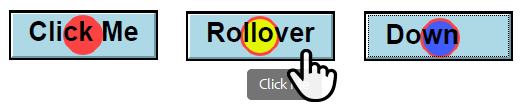
\includegraphics[scale=0.45]{figures/ch15/figure14}\caption{A button with images for different behavior.}\label{mar:behavior-pushA-button-with}
\end{marginfigure}
For example, in Listing \ref{lis:A-button-with} you add an image,
rollover image, and push image. First, you set the button's image using
the \texttt{Image}\index{Image} property. Then, you specify the button's \texttt{LabelImageLayout}\index{LabelImageLayout}
to be an overlay image using the \texttt{LabelImageLayoutOptions}\index{LabelImageLayoutOptions}.
Other \texttt{LabelImageLayoutOptions}\index{LabelImageLayoutOptions} include \texttt{LabelLeftImageRight}\index{LabelLeftImageRight},
\texttt{ImageOnly}\index{ImageOnly}, \texttt{LabelBottomImageTop}\index{LabelBottomImageTop}, \texttt{LabelOnly}\index{LabelOnly},
\texttt{LabelRightImageLeft}\index{LabelRightImageLeft}, \texttt{LabelTopImageBottom}\index{LabelTopImageBottom}, and \texttt{OverlayImage}\index{OverlayImage}.
You then use the \texttt{CreatePush}\index{CreatePush} method to add a rollover image
and a push image (Figure \ref{mar:behavior-pushA-button-with}).

\bgroup\inputencoding{latin9}
\begin{lstlisting}[caption={A button with images.},label={lis:A-button-with},basicstyle={\small\ttfamily},breaklines=true]
using ceTe.DynamicPDF;
using ceTe.DynamicPDF.Imaging;
using ceTe.DynamicPDF.PageElements.Forms;

namespace ChapterExamples.Chapters.ChapterFifteen
{
    public class ButtonBehaviorExample
    {
        public static void Create(string inputPath, string outputPath)
        {
            Document doc = new Document();
            doc.Pages.Add(new Page(PageSize.Letter));
            
            Button button = new Button("Submit", 100, 625, 75, 25);
            button.BackgroundColor = RgbColor.LightBlue;
            button.BorderStyle = BorderStyle.Beveled;
            button.Image = ImageData.GetImage(inputPath + "/button.png");
            button.LabelImageLayout = LabelImageLayoutOptions.OverlayImage;
            button.ImageAppearance.FitToBounds = true;
            
            button.Behavior = Behavior.CreatePush("Down", "Rollover", ImageData.GetImage(inputPath + "/push-down.png"), ImageData.GetImage(inputPath + "/rollover.png"));
            button.Label = "Click Me";
            
            doc.Pages[0].Elements.Add(button);
            doc.Draw(outputPath + "button-behavior-out.pdf");
        }
    }
}
\end{lstlisting}
\leavevmode\egroup


\section{Signature}

The final form field element we consider is the \texttt{Signature}\index{Signature}
field. We already saw this class when discussing security and digitally
signing a PDF document (Chapter \ref{subsec:Digitally-Signing}).
You can also use the \texttt{Signature}\index{Signature} class to allow the user of
a PDF to digitally sign the PDF, where the end-user provides the
certificate. 

In Listing \ref{lis:sig-Creating-a-simple} you create a form with
a \texttt{Signature}\index{Signature} element (Figure \ref{mar:A-Signature-element.}).
First, you create a checkbox and add it to the page. Then you add a
new \texttt{Signature}\index{Signature} instance. 
\begin{figure}

\includegraphics[scale=0.5]{figures/ch15/fig9}\caption{A Signature element.}\label{mar:A-Signature-element.}

\end{figure}
Note that here, unlike Chapter \ref{subsec:Digitally-Signing}, you
do not add a certificate, as you - the PDF creator - is not signing
the document, but rather, the end user is signing it.

\bgroup\inputencoding{latin9}
\begin{lstlisting}[caption={Creating a simple form with a Signature element.},label={lis:sig-Creating-a-simple},basicstyle={\small\ttfamily},breaklines=true]
using ceTe.DynamicPDF;
using ceTe.DynamicPDF.PageElements;
using ceTe.DynamicPDF.PageElements.Forms;

namespace ChapterExamples.Chapters.ChapterFifteen
{
    public class SignFormExample
    {
        public static void Create(string outputPath)
        {
            Document doc = new Document();
            doc.Pages.Add(new Page(PageSize.Letter));

            Label label = new("Final Report?", 0, 0, 100, 0);
            CheckBox checkBox = new("final_report", label.Width + 5, 0, 20, 20);
            checkBox.DefaultChecked = false;
            checkBox.ToolTip = "Check if this is final report.";
            doc.Pages[0].Elements.Add(label);
            doc.Pages[0].Elements.Add(checkBox);

            Label label2 = new("Signature:",0, 50, 100, 0);
            Signature signature = new("user_signature", 100, 50, 300, 100);
            doc.Pages[0].Elements.Add(label2);
            doc.Pages[0].Elements.Add(signature);
            doc.Draw(outputPath + "signature-form-out.pdf");
        }
    }
}
\end{lstlisting}
\leavevmode\egroup
When a user of the PDF clicks the signature field, they are prompted
to select the certificate they wish to sign with. If a user does not
have a digital ID they are allowed to create one (Figure \ref{fig:Signing-a-completed}).
\begin{figure}

\includegraphics[scale=0.25]{figures/ch15/fig10}\caption{Signing a completed form.}\label{fig:Signing-a-completed}

\end{figure}

The user is provided several options to sign the PDF, including using
an image on their hard-drive or signing freehand (Figure \ref{fig:Dialogues-signing-a}).
\begin{figure}

\includegraphics[scale=0.35]{figures/ch15/fig11}\caption{Dialog signing a form.}\label{fig:Dialogues-signing-a}
\end{figure}
 After signing, the user then saves the PDF as a different document.
The new document is then the completed PDF document (Figure \ref{fig:Opening-the-signed}).
\begin{figure}

\includegraphics[scale=0.25]{figures/ch15/fig12}\caption{Opening the signed document.}\label{fig:Opening-the-signed}

\end{figure}

\section{AutoLayout}
\label{section:autolayout-forms}
You can use the \texttt{AutoLayout}\index{AutoLayout} class to add form elements automatically to a \texttt{Document} instance just as you can other page elements (see Chapters \ref{sec:autolayout}, \ref{section:autolayout-shape}, \ref{section:autolayout-image}, \ref{section:autolayout-table}, \ref{section:autolayout-charts}). The following example illustrates (Listing \ref{lis:autolayout-forms}).

\bgroup\inputencoding{latin9}
\begin{lstlisting}[caption={Using AutoLayout to create a PDF document.},label={lis:autolayout-forms},basicstyle={\small\ttfamily},breaklines=true]

using ceTe.DynamicPDF;
using ceTe.DynamicPDF.PageElements;
using ceTe.DynamicPDF.PageElements.Forms;

namespace ChapterExamples.Chapters.ChapterFifteen
{
    public class AutoLayoutExampleForms
    {
        public static void Create(string outputPath)
        {
            AutoLayout autoLayout = new AutoLayout(PageSize.Letter, PageOrientation.Portrait, 50);
            TextField textField = autoLayout.AddTextField("Description", 75, 150);
            textField.BorderStyle = BorderStyle.Solid;
            textField.MultiLine = true;
            ListBox listBox = autoLayout.AddListBox("Selected Days", 150, 100);
            listBox.Items.Add("Mon", true);
            listBox.Items.Add("Tue");
            listBox.Items.Add("Wed");
            listBox.BorderStyle = BorderStyle.Solid;

            Document document = autoLayout.GetDocument();
            document.Draw(outputPath + "autolayout-output.pdf");
        }
    }
}

\end{lstlisting}
\leavevmode\egroup

\section{Summary}

In this chapter, you learned how to use DynamicPDF Core Suite
for .NET to create interactive forms that include text fields, drop-down
menus, radio buttons, check-boxes, and several other form elements.
We discussed the \texttt{FormElement} parent class and then each of
its child classes, starting with the \texttt{CheckBox}. After learning
how to add \texttt{CheckBox} to a PDF form, you then learned how to
add radio buttons (\texttt{RadioButton}), text fields (\texttt{TextField}),
list boxes (\texttt{ListBox}), combo boxes (\texttt{ComboBox}), buttons
(\texttt{Button}), and signature (\texttt{Signature}) fields to a
form. Remember to use the form fields from the \texttt{ceTe.DynamicPDF.PageElements.Forms}
namespace and not the \texttt{ceTe.DynamicPDF.Forms} namespace, as
the Forms namespace is used when completing or modifying a preexisting
PDF document, not creating a PDF document.

Now that we have learned how to create interactive forms, lets examine
how to make PDF documents interative for end-users of a PDF. We first
discuss events that you can handle with actions. We then discuss the
actions Core Suite provides and learn how to use them. 

\color{white}
\chapter{Making PDFs Interactive}\label{chap:Actions-and-Events}
\color{black}
\BgThispage
\vspace{8.0em}
\lettrine[lines=2,lhang=0.1]{E}{vent-driven} programming (EDP) focuses on events an application listens
for and responds to with an action. You can create highly responsive
and scalable applications by handling events using actions. Event-driven
programming enables components to react to events. An application's
flow is determined by events such as user actions, system changes,
and other sources. In event-driven programming, the program waits
for and responds to these events.

DynamicPDF Core Suite for .Net provides events for a PDF's document,
page, and form (Table \ref{tab:Available-events-for}). Core Suite
also has actions to handle these events (Table \ref{mar:Core-Suite-Actions.}).
In this chapter, we discuss the events provided by Core Suite and
the actions available to handle them. By chapter's end, you will have
learned how to add code to a PDF so that end users can respond to
events triggered when the user interacts with a PDF.

\section{Events}

Events help determine a program's flow by reacting to external events.
An event is usually handled by an action performed in response to
an event. For instance, a user clicks a button, which fires a mouse-down
and mouse-up event, and the program can respond to each event by performing
one or more actions. DynamicPDF Core Suite for .Net provides events
when printing, saving, opening and closing documents, and when an
end-user moves their mouse or interacts with a form element. Table
\ref{tab:Available-events-for} lists the events provided by Core
Suite.

\begin{table}[h]
\begin{tabular}{ll}
\toprule 
{\small Event} & \tabularnewline
\midrule
\multicolumn{2}{c}{{\small Document (}{\small\texttt{DocumentReaderEvent}}{\small s)}}\tabularnewline
 & \tabularnewline
{\small\texttt{DidPrint}} & {\small Triggered after printing.}\tabularnewline
{\small\texttt{DidSave}} & {\small Triggered after saving.}\tabularnewline
{\small\texttt{WillClose}} & {\small Triggered just before closing.}\tabularnewline
{\small\texttt{WillPrint}} & {\small Fired just before printing.}\tabularnewline
{\small\texttt{WillSave}} & {\small Triggered just before saving.}\tabularnewline
 & \tabularnewline
\multicolumn{2}{c}{{\small Page (}{\small\texttt{PageReaderEvent}}{\small s)}}\tabularnewline
 & \tabularnewline
{\small\texttt{Open}} & {\small Triggered when page opened.}\tabularnewline
{\small\texttt{Close}} & {\small Triggered when page closed.}\tabularnewline
 & \tabularnewline
\multicolumn{2}{c}{{\small Form (}{\small\texttt{AnnotationReaderEvent}}{\small s)}}\tabularnewline
 & \tabularnewline
{\small\texttt{MouseDown}} & {\small Triggered when mouse button pressed.}\tabularnewline
{\small\texttt{MouseEnter}} & {\small Triggered when mouse enters field.}\tabularnewline
{\small\texttt{MouseExit}} & {\small Triggered when mouse exits field.}\tabularnewline
{\small\texttt{MouseUp}} & {\small Triggered when mouse button released.}\tabularnewline
{\small\texttt{OnBlur}} & {\small Triggered when field loses focus.}\tabularnewline
{\small\texttt{OnFocus}} & {\small Triggered when field gains focus.}\tabularnewline
\bottomrule
\end{tabular}\caption{Available events for Core Suite.}\label{tab:Available-events-for}

\end{table}


\subsection{Reader Events}

Core Suite provides three types of reader events, \texttt{DocumentReaderEvents}\index{DocumentReaderEvents},
\texttt{PageReaderEvents}\index{PageReaderEvents}, and \texttt{AnnotationReaderEvents}\index{AnnotationReaderEvents}. As
Table \ref{tab:Available-events-for} illustrates, \texttt{AnnotationReaderEvents}\index{AnnotationReaderEvents}
occur when a user interacts with a form element. \texttt{DocumentReader}\index{DocumentReader}
events occur when a user interacts with a PDF document. And \texttt{PageReaderEvents}\index{PageReaderEvents}
occur when a page is opened or closed.

Each class: \texttt{Document}, \texttt{Page}, and \texttt{Form} has
a \texttt{ReaderEvents}\index{ReaderEvents} property that takes its respective reader
event type. For example, upon opening a page, a \texttt{PageReaderEvent}\index{PageReaderEvent}
event is fired and can be handled by one or more actions (\bgroup\inputencoding{latin9}\lstinline[basicstyle={\small\ttfamily},breaklines=true]!document.ReaderEvents.Open = <an-action>;!\egroup
).\marginnote{In this section we use a JavaScriptAction to illustrate event
handling. We cover JavaScript actions in Chapter \ref{chap:Using-JavaScript},
but its use here should prove intuitive.}

\subsection{Document Events}

The \texttt{Document} class handles the following events: \texttt{DidPrint}\index{DidPrint},
\texttt{DidSave}\index{DidSave}, \texttt{WillClose}\index{WillClose}, \texttt{WillPrint}\index{WillPrint}, and \texttt{WillSave}\index{WillSave}.
You handle these events by setting an action to handle the event,
Listing \ref{lis:Document-events.} illustrates. Listing \ref{lis:Document-events.}
handles all document level events with a simple \texttt{JavaScriptAction}\index{JavaScriptAction}
that opens an alert that tells the user what event was triggered (Figure
\ref{fig:Document-events.}). 
\begin{figure}

\includegraphics[scale=0.37]{figures/ch16/fig1}\caption{Document events - printing a PDF document.}\label{fig:Document-events.}
\end{figure}

\bgroup\inputencoding{latin9}
\begin{lstlisting}[caption={Document events.},label={lis:Document-events.},basicstyle={\small\ttfamily},breaklines=true]
public static void DocumentReaderEventsExample(string outputPath)
{
    Document doc = new();
    doc.Pages.Add(new Page(PageSize.Letter));
            
    JavaScriptAction action = new JavaScriptAction("app.alert(\"WillSave\")");
    doc.ReaderEvents.WillSave = action;
    JavaScriptAction action2 = new JavaScriptAction("app.alert(\"WillClose\")");
    doc.ReaderEvents.WillClose = action2;
    JavaScriptAction action3 = new JavaScriptAction("app.alert(\"WillPrint\")");
    doc.ReaderEvents.WillPrint = action3;

    JavaScriptAction action4 = new JavaScriptAction("app.alert(\"DidSave\")");
    doc.ReaderEvents.DidSave = action;
    JavaScriptAction action5 = new JavaScriptAction("app.alert(\"DidPrint\")");
    doc.ReaderEvents.DidPrint = action5;

    doc.Draw(outputPath + "document-readerevent-out.pdf");
}
\end{lstlisting}
\leavevmode\egroup

As Figure \ref{fig:Document-events.} illustrates, when a user attempts
to save a document, it triggers the \texttt{WillSave}\index{WillSave} event which
is then handled by a \texttt{JavaScriptAction}\index{JavaScriptAction} that prints a message
to the user telling them the application is about to save the document.
The other events likewise perform a \texttt{JavaScriptAction}\index{JavaScriptAction} that
presents the user with an alert message.

\subsection{Page Events}

Page events occur when a user navigates to or from a particular page
in a PDF document. The \texttt{Page}\index{Page} class handles the \texttt{Open}\index{Open}
and \texttt{Close}\index{Close} events. Listing \ref{lis:Page-events.} illustrates
handling these two events. It sets the page's \texttt{ReaderEvents}\index{ReaderEvents}
property to handle the \texttt{Open}\index{Open} and \texttt{Close}\index{Close} events with
a JavaScript alert that informs the user if the page was opened or
closed (Figure \ref{fig:Page-events.}).

\bgroup\inputencoding{latin9}
\begin{lstlisting}[caption={Page events.},label={lis:Page-events.},basicstyle={\small\ttfamily},breaklines=true]
public static void PageReaderEventsExample(string outputPath)
{
    Document doc = new();
    doc.Pages.Add(new Page(PageSize.Letter));
    doc.Pages.Add(new Page(PageSize.Letter));
            
    JavaScriptAction action = new JavaScriptAction("app.alert(\"Open\")");
    doc.Pages[1].ReaderEvents.Open = action;

    JavaScriptAction action2 = new JavaScriptAction("app.alert(\"Close\")");
    doc.Pages[1].ReaderEvents.Close = action2;
    doc.Draw(outputPath + "page-readerevents-out.pdf");
}
\end{lstlisting}
\leavevmode\egroup

\begin{figure}

\includegraphics[scale=0.4]{figures/ch16/fig2}\caption{Page events.}\label{fig:Page-events.}

\end{figure}


\subsection{Form Events}

Form events occur when a user performs one of the following actions
when interacting with any of the form field elements: \texttt{MouseDown}\index{MouseDown},
\texttt{MouseEnter}\index{MouseEnter}, \texttt{MouseExit}\index{MouseExit}, \texttt{MouseUp}\index{MouseUp}, \texttt{OnBlur}\index{OnBlur},
and \texttt{OnFocus}\index{OnFocus}. Listing \ref{lis:Form-field-events.} illustrates
handling the \texttt{OnFocus}\index{OnFocus} and \texttt{MouseDown}\index{MouseDown} events provided
by the \texttt{AnnotationFieldReaderEvents}\index{AnnotationFieldReaderEvents} (Figure \ref{fig:Form-field-events.}).

\bgroup\inputencoding{latin9}
\begin{lstlisting}[caption={Form field events.},label={lis:Form-field-events.},basicstyle={\small\ttfamily},breaklines=true]
public static void FormFieldEventsExample()
{
    Document document = new Document();
    document.Pages.Add(new Page(PageSize.Letter));

    Label label = new Label("Check Box:", 0, 10, 100, 0);
    CheckBox checkBox = new CheckBox("check_box_nm", 110, 7, 50, 50);
    checkBox.DefaultChecked = true;
    checkBox.ToolTip = "Check it";

    JavaScriptAction action = new JavaScriptAction("app.alert(\"focus !!\")");
    checkBox.ReaderEvents.OnFocus = action;

    JavaScriptAction action2 = new JavaScriptAction("app.alert(\"mouse-down !!\")");
    checkBox.ReaderEvents.MouseDown = action2;

    document.Pages[0].Elements.Add(label);
    document.Pages[0].Elements.Add(checkBox);

    document.Draw(Util.GetPath("Output/form-reader-events-output.pdf"));
}
\end{lstlisting}
\leavevmode\egroup

\begin{figure}

\includegraphics[scale=0.23]{figures/ch16/fig3}\caption{Form field events.}\label{fig:Form-field-events.}
\end{figure}


\section{Actions}\label{sec:Actions}

You handle events using actions. Core suite provides the following
actions: \texttt{URLAction}\index{URLAction}, \texttt{SubmitAction}\index{SubmitAction}, \texttt{GoToAction}\index{GoToAction},
\texttt{AnnotationShowHideAction}\index{AnnotationShowHideAction}, \texttt{FileOpenAction}\index{FileOpenAction}, \texttt{ImportFormDataAction}\index{ImportFormDataAction},
\texttt{ResetAction}\index{ResetAction}, and \texttt{JavaScriptAction}\index{JavaScriptAction}. All actions inherit
from the abstract \texttt{Action}\index{Action} class thus allowing any event to
perform any action.

\begin{table}
\begin{tabular}{ll}
\toprule 
{\footnotesize Action} & \tabularnewline
\midrule
{\footnotesize\texttt{URLAction}} & {\footnotesize Navigate to a specified URL.}\tabularnewline
{\footnotesize\texttt{SubmitAction}} & {\footnotesize Submit a form to HTML POST or GET.}\tabularnewline
{\footnotesize\texttt{GoToAction}} & {\footnotesize Navigate to another page in a PDF document.}\tabularnewline
{\footnotesize\texttt{AnnotationShowHideAction}} & {\footnotesize Show or hide a form field.}\tabularnewline
{\footnotesize\texttt{ResetAction}} & {\footnotesize Reset form field values of a form.}\tabularnewline
{\footnotesize\texttt{FileOpenAction}} & {\footnotesize Open a file.}\tabularnewline
{\footnotesize\texttt{ImportFormDataAction}} & {\footnotesize Import form data to a form.}\tabularnewline
\bottomrule
\end{tabular}\caption{Core Suite Actions.}\label{mar:Core-Suite-Actions.}
\end{table}


\subsection{Hiding/Showing Form Fields}

Hiding and showing form fields is straightforward using the {\texttt{AnnotationShowHideAction}\index{AnnotationShowHideAction}
class. By default an action hides the form field; however the class
also has a \texttt{ShowField}\index{ShowField} property that allows
hiding or showing the field. Listing \ref{lis:Hiding-and-showing}
illustrates hiding and showing a form field. Upon clicking a button
labeled "Hide" the form field is hidden. Upon clicking a button
labeled "Show" the form field is displayed.
\begin{marginfigure}

\includegraphics[scale=0.20]{figures/ch16/fig4}\caption{Hiding and showing a form field.}\label{fig:Hiding-and-showing}
\end{marginfigure}

\bgroup\inputencoding{latin9}
\begin{lstlisting}[caption={Hiding and showing a form field.},label={lis:Hiding-and-showing},basicstyle={\small\ttfamily},breaklines=true]
public static void AnnotationShowHideActionExample(string outputPath)
{
  Document doc = new Document();
    doc.Pages.Add(new Page(PageSize.Letter));

    Label label2 = new Label("Name:", 0, 50, 75, 0);
    TextField textField = new TextField("Text1", 75, 50, 200, 20);
    textField.DefaultValue = "Text Field Value";
    doc.Pages[0].Elements.Add(label2);
    doc.Pages[0].Elements.Add(textField);

    Button button = new Button("btn", 50, 150, 100, 30);
    button.Label = "Hide";
          
    AnnotationShowHideAction action = new AnnotationShowHideAction("Text1");
    button.ReaderEvents.MouseDown = action;

    Button button2 = new Button("btn", 175, 150, 100, 30);
    button2.Label = "Show";

    AnnotationShowHideAction action2 = new AnnotationShowHideAction("Text1");
    action2.ShowField = true;
    button2.ReaderEvents.MouseDown = action2;

    doc.Pages[0].Elements.Add(button);
    doc.Pages[0].Elements.Add(button2);

    doc.Draw(outputPath + "annotation-show-hide-action-output.pdf");
}
\end{lstlisting}
\leavevmode\egroup


\subsection{Navigating to a URL}

We already saw the\texttt{UrlAction}\index{UrlAction} at work in Chapter
\ref{chap:Adding-Bookmarks-and}. A \texttt{UrlAction}\index{UrlAction},
like the \texttt{ResetAction}\index{ResetAction}, does exactly what you
would expect it to - navigate to a specified URL. Listing \ref{lis:url-Navigating-to-a}
illustrates navigating to a URL upon clicking a button.

\bgroup\inputencoding{latin9}
\begin{lstlisting}[caption={Navigating to a URL using UrlAction.},label={lis:url-Navigating-to-a},basicstyle={\small\ttfamily},breaklines=true]
public static void UrlActionExample(string outputPath)
{
  Document doc = new Document();
    doc.Pages.Add(new Page(PageSize.Letter));

    string text = "This is a link to DynamicPDF API.";

    Label label = new Label(text, 50, 20, 215, 80);
    label.Underline = true;
    Link link = new(50, 20, 150, 20, new UrlAction("https://dpdf.io/"));

    UrlAction action = new UrlAction("http://www.dynamicpdf.com");
    Button button = new Button("btn", 50, 100, 100, 50);
    button.Label = "Click";
    button.Action = action;

    doc.Pages[0].Elements.Add(label);
    doc.Pages[0].Elements.Add(link);
    doc.Pages[0].Elements.Add(button);
    doc.Draw(outputPath + "url-navigate-action-output.pdf");
}
\end{lstlisting}
\leavevmode\egroup


\subsection{Navigating to a Page}

The \texttt{GoToAction}\index{GoToAction} goes to a page indicated by
the action. It also allows zooming by a certain percentage after navigating
to the linked page. Listing \ref{lis:Navigating-to-page} illustrates
navigating to the second page upon pushing a button on the first page.
\begin{figure}

\includegraphics[scale=0.2]{figures/ch16/fig5}\caption{Navigating to a page using GoToAction.}\label{fig:Navigating-to-a}
\end{figure}

\bgroup\inputencoding{latin9}
\begin{lstlisting}[caption={Navigating to page using GoToAction.},label={lis:Navigating-to-page},basicstyle={\small\ttfamily},breaklines=true,showstringspaces=false]
public static void GoToActionExample(string outputPath)
{
  Document doc = new Document();
    doc.Pages.Add(new Page(PageSize.Letter));
    doc.Pages.Add(new Page(PageSize.Letter));
    doc.Pages[0].Elements.Add(new Label("Page 1", 0, 0, 100, 15));
    doc.Pages[1].Elements.Add(new Label("Page 2", 0, 0, 100, 15));
            
    Button button = new Button("btn", 50, 150, 100, 30);
    button.Label = "Change Page";
    GoToAction action = new GoToAction(2, PageZoom.FitWidth);
    button.ReaderEvents.MouseUp = action;

    doc.Pages[0].Elements.Add(button);
    doc.Draw(outputPath + "go-to-action-output.pdf");
}
\end{lstlisting}
\leavevmode\egroup


\cprotect\subsection{Opening a File
\begin{marginfigure}
\protect
\includegraphics[scale=0.4]{figures/ch16/fig6}\protect\caption{Opening a file with \texttt{FileOpenAction}\index{FileOpenAction}.}\label{mar:Opening-a-file}
\end{marginfigure}
}

Open a file using the \texttt{FileOpenAction}\index{FileOpenAction} action.
This class's constructor takes a file path and a \texttt{FileLaunchMode}\index{FileLaunchMode}
enumeration. Launch modes include \texttt{ExistingWindow}\index{ExistingWindow}, \texttt{NewWindow}\index{NewWindow},
and \texttt{UserPreference}\index{UserPreference}. Listing \ref{lis:Opening-a-file} illustrates
opening a file upon clicking a button.

\bgroup\inputencoding{latin9}
\begin{lstlisting}[caption={Opening a file with FileOpenAction.},label={lis:Opening-a-file},basicstyle={\small\ttfamily},breaklines=true]
public static void FileOpenActionExample(string inputPath, string outputPath)
{
  Document doc = new Document();
    doc.Pages.Add(new Page(PageSize.Letter));
         
    Button button = new Button("btn", 50, 150, 100, 30);
    button.Label = "Open File";
    FileOpenAction action = new FileOpenAction(inputPath, FileLaunchMode.NewWindow);
    button.ReaderEvents.MouseUp = action;

    doc.Pages[0].Elements.Add(button);
    doc.Draw(outputPath + "file-open-action-output.pdf");
}
\end{lstlisting}
\leavevmode\egroup


\subsection{Resetting Form Data}

The \texttt{ResetAction}\index{ResetAction} does exactly what you expect
it to do - it resets all a form's form fields to their default values
(Listing \ref{lis:Resetting-a-form's}). For example, when the button
in Listing \ref{lis:Resetting-a-form's} is clicked, it resets the
text field to its default value (Figure \ref{mar:Resetting-a-form's}).
\begin{marginfigure}

\includegraphics[scale=0.3]{figures/ch16/fig7}\caption{Resetting a form's values using ResetAction.}\label{mar:Resetting-a-form's}

\end{marginfigure}

\bgroup\inputencoding{latin9}
\begin{lstlisting}[caption={Resetting a form's values using ResetAction.},label={lis:Resetting-a-form's},basicstyle={\small\ttfamily},breaklines=true]
public static void ResetActionExample(string outputPath)
{
    Document doc = new Document();
    doc.Pages.Add(new Page(PageSize.Letter));

    Label label2 = new Label("Name:", 0, 50, 75, 0);
    TextField textField = new TextField("text_field", 75, 50, 200, 20);
    textField.DefaultValue = "default text value";
    doc.Pages[0].Elements.Add(label2);
    doc.Pages[0].Elements.Add(textField);

    Button button = new Button("btn", 50, 150, 100, 30);
    button.Label = "Reset";
    ResetAction action = new ResetAction();
    button.ReaderEvents.MouseUp = action;

    doc.Pages[0].Elements.Add(button);
    doc.Draw(outputPath + "reset-action-output.pdf");
}
\end{lstlisting}
\leavevmode\egroup
\subsection{Importing Form Data}
The \texttt{ImportFormDataAction}\index{ImportFormDataAction}, as with the last two actions, functions exactly as you expect this action to perform. Upon the action being performed, the PDF document opens an FDF file (Figure \ref{mar:form-fill}) and completes the form with the FDF data. 
\begin{marginfigure}

\includegraphics[scale=0.38]{figures/ch16/fig9}\caption{Importing form data.}\label{mar:form-fill}
\end{marginfigure}
Listing \ref{lis:import-form-data} illustrates. You build a form and then for the action you attach a new \texttt{ImportFormDataAction}\index{ImportFormDataAction} instance to the button's \texttt{MouseUp}\index{MouseUp} event.
\bgroup\inputencoding{latin9}
\begin{lstlisting}[caption={Importing form data.},label={lis:import-form-data},basicstyle={\small\ttfamily},breaklines=true]
public static void ImportFormDataExample(string fileInput, string outputPath)
{
     Document doc = new Document();
  doc.Pages.Add(new Page(PageSize.Letter));
  Label lbl1 = new Label("Name:", 0, 0, 100, 30);
  TextField textField = new TextField("text_field", 50, 0, 200, 20);
  Label lbl2 = new Label("Completed:", 0, 50, 75, 0);
  CheckBox chkBox = new CheckBox("check_field", 75, 50, 20, 20);
  Button btn = new Button("btn", 0, 100, 100, 30);
  button.Label = "Import Data";
  doc.Pages[0].Elements.Add(lbl1);
  doc.Pages[0].Elements.Add(lbl2);
  doc.Pages[0].Elements.Add(textField);
  doc.Pages[0].Elements.Add(chkBox);
  doc.Pages[0].Elements.Add(btn);
  ImportFormDataAction action = new ImportFormDataAction("c:/temp/import-form-data-action-data.fdf");
  button.ReaderEvents.MouseUp = action;
  doc.Draw(outputPath + "import-form-data-action-output.pdf");
}
\end{lstlisting}
\leavevmode\egroup
\begin{figure}

\includegraphics[scale=0.55]{figures/ch16/fig8}\caption{Importing form data.}\label{fig:Navigating-to-a}
\end{figure}
\subsection{Action Chaining}

The final topic in this chapter is chaining multiple actions together.
You can chain two or more actions to perform various actions in sequence
when an event is triggered. Recall that all actions are children of
the \texttt{Action}\index{Action} class; regardless of the event, any action can be used
as the handler. Any event can handle any action.

Chaining multiple actions is straightforward, as Listing \ref{lis:Chaining-multiple-actions}
illustrates. In Listing \ref{lis:Chaining-multiple-actions} you create
a text field and a button and add a \texttt{ResetAction}\index{ResetAction} instance
to both element's \texttt{MouseUp}\index{MouseUp} event. After creating the PDF document,
upon opening, the PDF navigates to page two upon clicking the button,
and a file is opened. 

\bgroup\inputencoding{latin9}
\begin{lstlisting}[caption={Chaining multiple actions in a PDF document.},label={lis:Chaining-multiple-actions},basicstyle={\small\ttfamily},breaklines=true]
public static void ChainActionExample(string inputPath, string outputPath)
{
  Document doc = new Document();
    doc.Pages.Add(new Page(PageSize.Letter));
    doc.Pages.Add(new Page(PageSize.Letter));

    TextField textField = new TextField("text_field", 0, 50, 200, 20);
    textField.DefaultValue = "default text value";

    Button button = new Button("btn", 0, 150, 100, 30);
    button.Label = "Chain";

    doc.Pages[0].Elements.Add(new Label("Page 1", 0, 0, 100, 15));
    doc.Pages[1].Elements.Add(new Label("Page 2", 0, 0, 100, 15));

    doc.Pages[0].Elements.Add(textField);
    doc.Pages[0].Elements.Add(button);

    ResetAction action = new ResetAction();
    button.ReaderEvents.MouseUp = action;

    action.NextAction = new GoToAction(2, PageZoom.FitWidth);
    action.NextAction = new FileOpenAction(inputPath, FileLaunchMode.NewWindow);

    doc.Draw(outputPath + "chain-action-output.pdf");
}
\end{lstlisting}
\leavevmode\egroup


\section{Summary}

In this chapter, you learned about the events provided by the Core Suite and the actions used to handle them. Specifically, you explored how to handle \texttt{DocumentReaderEvents}\index{DocumentReaderEvents}, \texttt{PageReaderEvents}\index{PageReaderEvents}, and \texttt{AnnotationFieldReaderEvents}\index{AnnotationFieldReaderEvents}. As demonstrated, DynamicPDF Core Suite for .NET provides events for a PDF’s document, pages, and forms (see Table \ref{tab:Available-events-for}).

After covering events, we examined the available actions for handling them. You learned how to use these actions to hide or show form fields, navigate to a URL or a specific page, open a file, reset form data, and import data into a form. Additionally, you saw how to chain multiple actions together to handle an event effectively.

One action we did not discuss in depth is the \texttt{JavaScriptAction}\index{JavaScriptAction} class. Although we briefly used it in event-handling examples, we did not explore it when covering actions. Instead, we will focus on this class in the next chapter, where we discuss integrating JavaScript into PDF documents. As you will see, adding JavaScript allows end users to interact dynamically with your PDFs.

\color{white}
\chapter{Using JavaScript}\label{chap:Using-JavaScript}
\color{black}
\BgThispage
\vspace{8.00em}
\lettrine[lines=2,lhang=0.1]{I}{n} this chapter, you learn how to add JavaScript to your PDF documents.
This is not a chapter on programming PDFs using JavaScript, as that
would fill an entire book. However, this chapter does discuss how
to integrate JavaScript into the PDF documents you create using Core
Suite. You can incorporate JavaScript into your PDF documents at the
document level and to specific form elements using the \texttt{DocumentJavaScript}\index{DocumentJavaScript}
and \texttt{JavaScriptAction}\index{JavaScriptAction} classes.

JavaScript is beneficial for adding interactivity to interactive
forms. Validating a form's data, formatting a form's data, and performing
calculations are all simple tasks when using JavaScript. In this chapter,
you learn how to do all these tasks using JavaScript, so let's
begin.

\section{Run-Time PDF Functionality}

For junior developers, the distinction between code used to generate a PDF and code used to enable interactivity at runtime is not always clear. JavaScript, a lightweight, interpreted programming language, is commonly embedded in HTML pages to manipulate the Document Object Model (DOM). The DOM represents an HTML or XML document as a logical tree structure of nodes, allowing JavaScript to dynamically modify a page’s content, style, and structure. Nodes can also have event handlers that trigger specific actions when activated.

Unlike HTML documents, PDFs do not have a DOM or native support for interactivity via JavaScript. However, most PDF readers, including Adobe Acrobat, have built-in JavaScript interpreters that allow for interactive functionality. Core Suite is solely responsible for generating PDFs—once a PDF is created, Core Suite has no embedded interpreter for runtime interactions. Instead, any interactivity must be handled using JavaScript within the user's PDF reader.

Adobe Acrobat products use JavaScript for various tasks, including processing forms, executing batch operations, interacting with databases, and controlling multimedia. However, before implementing JavaScript in a PDF, you must ensure the reader software your users rely on supports the specific JavaScript features you plan to use. Different properties and functions have varying restrictions, and failing to check Adobe’s documentation can lead to significant debugging challenges.

Adobe’s documentation specifies access restrictions for each JavaScript property and function. For example, you might want to add a button that deletes two pages from a PDF when clicked. While calling \texttt{doc.deletePages(2, 1);} might seem straightforward, this function also requires form rights to be enabled in the PDF, making using the function more complex then appears. Understanding these restrictions in advance can save considerable troubleshooting time.
\begin{marginfigure}

\includegraphics[scale=0.35]{figures/ch17/fig12}\caption{JavaScript method that requires forms rights.}\label{mar:forms-rights-JavaScript-method-that}

\end{marginfigure}
 Assigning rights requires creating a rights-enabled document, and
creating a rights-enabled document requires understanding Adobe's
Reader Extensions. Moreover, you apply usage rights to PDF documents
using the Acrobat Reader DC extensions Java Client API and web service,
both of which are part of Adobe's Experience Manager (AEM). Adobe
Experience Manager is a content management system (CMS) and digital
asset management (DAM) system for enterprise organizations. After
using AEM to assign the required rights to a document, any user who
opens the document in Adobe Reader can perform the enabled operations
for that document.\sidenote{Refer to the topic Assigning Usage Rights in Adobe's Experience Manager
documentation.}

AEM is beyond this book's scope. Moreover, for most readers, AEM is
prohibitively expensive and probably overkill for your organization's
needs which are creating PDF documents and not using enterprise document
management solutions. Therefore, in this chapter, we assume our end-users
are only using Adobe Acrobat Reader, and we only use JavaScript without
rights restrictions.

\section{DocumentJavaScript}

All PDF documents start with the \texttt{Doc}\index{Doc} object and can be referred
to using the \texttt{this} keyword. For example, \texttt{this.author}
refers to a PDF's author (Figure \ref{mar:Console-printout-of}).\bgroup\inputencoding{latin9}
\begin{lstlisting}[basicstyle={\small\ttfamily},breaklines=true]
console.println("Author " + this.author);
\end{lstlisting}
\leavevmode\egroup
Use the keyword \texttt{this} to refer to the \texttt{Doc}\index{Doc} object.
The \texttt{Doc}\index{Doc} object is the PDF document's root object and provides
methods and properties for accessing the PDF document. Access the
documentation for the \texttt{Doc}\index{Doc} object at Adobe's Acrobat JavaScript
API Reference. But, as discussed in the previous section, be certain
of the property or method's privileged context (user rights).

You can add JavaScript to a document using Core Suite's \texttt{DocumentJavaScript}\index{DocumentJavaScript}
class. This class places JavaScript at the document's top-level. To
accomplish this, add a \texttt{DocumentJavaScript}\index{DocumentJavaScript} instance to your
\texttt{Document} instance's \texttt{JavaScripts}\index{JavaScripts} property. This property
is a \texttt{DocumentJavaScriptList}\index{DocumentJavaScriptList} object that contains any \texttt{DocumentJavaScript}\index{DocumentJavaScript}
instances you add using its \texttt{Add} method.
\begin{figure}

\includegraphics[scale=0.4]{figures/ch17/fig11}\caption{Console printout of document author.}\label{mar:Console-printout-of}
\end{figure}

Let's illustrate using the \texttt{DocumentJavaScript}\index{DocumentJavaScript} class by adding
some document level JavaScript that prints to the JavaScript Console.
But before beginning, if you only have Adobe Acrobat Reader and not
professional, you can enable the JavaScript debugger by adding this
code to a JavaScript file in Reader's \texttt{JavaScripts}\index{JavaScripts} folder.
This change then allows you to view the console if you wish to send
debugging messages. Unfortunately, it is only useful for logging console
messages or viewing error messages, as the free Acrobat Reader does
not allow interactive debugging, for that you need Acrobat Pro.

\bgroup\inputencoding{latin9}
\begin{lstlisting}[basicstyle={\small\ttfamily},breaklines=true]
app.addMenuItem({ cName: "ShowConsole", cUser: "Show &JS Console", cParent: "Window", nPos: -1, cExec: "console.show()", cEnable: "event.rc = (true);"});
\end{lstlisting}
\leavevmode\egroup

Listing \ref{lis:Accessing-Doc-object} illustrates using JavaScript
to print to the console when an end-user opens a PDF document. We
first create the JavaScript the PDF reader will execute. Next, we
create a new \texttt{DocumentJavaScript}\index{DocumentJavaScript} instance and pass the JavaScript
as a string to the instance's constructor. We then add the instance
to the \texttt{Document} instance's \texttt{JavaScripts}\index{JavaScripts} collection.
Note that the \texttt{on\_load} in the \texttt{DocumentJavaScript}\index{DocumentJavaScript}
instance's constructor is a name used to identify the instance and
has no special syntactical significance.

After creating the PDF, when we open it and review the \textbf{JavaScript
Console} window we see the messages written to the console (Figure
\ref{mar:Accessing-DOM-using}).
\begin{marginfigure}

\includegraphics[scale=0.4]{figures/ch17/fig1}\caption{Accessing DOM using JavaScript.}\label{mar:Accessing-DOM-using}
\end{marginfigure}

\bgroup\inputencoding{latin9}
\begin{lstlisting}[caption={Accessing Doc object in Adobe Acrobat using JavaScript.},label={lis:Accessing-Doc-object},basicstyle={\small\ttfamily},breaklines=true]
using ceTe.DynamicPDF;

namespace ChapterExamples.Chapters.ChapterSeventeen
{
    public class JavasScriptDomExample
    {
        public static void Create(string outputPath)
        {
            Document doc = new();
            doc.Pages.Add(new Page(PageSize.Letter));
            doc.Pages.Add(new Page(PageSize.Letter));
            doc.Pages.Add(new Page(PageSize.Letter));

            string javascriptString = "console.println('Adobe Acrobat console.');";
            javascriptString += "console.println('page count from DynamicPdf " + doc.Pages.Count + "');";
            javascriptString += "console.println('page count from JavaScript ' + this.numPages);";
            doc.JavaScripts.Add(new DocumentJavaScript("on_load", javascriptString));

            doc.Draw(outputPath + "simple-dom-javascript-output.pdf");
        }
    }
}
\end{lstlisting}
\leavevmode\egroup

We placed the JavaScript at the top-level rather than creating a method
and so it is executed by the PDF document upon being opened.\sidenote{We illustrate using a JavaScript function later in this chapter.}\bgroup\inputencoding{latin9}
\begin{lstlisting}[basicstyle={\small\ttfamily},breaklines=true]
console.println('Adobe Acrobat console.');
console.println('page count from DynamicPdf 2');
console.println('page count from JavaScript ' + this.numPages);
\end{lstlisting}
\leavevmode\egroup

Listing \ref{lis:Accessing-Doc-object} is admittedly a trivial example.
But as you will see in Listing \ref{lis:function-Using-document-level},
where it defines a JavaScript function and then later uses that function
in a \texttt{JavaScriptAction}\index{JavaScriptAction}, the \texttt{DocumentJavaScript}\index{DocumentJavaScript} class
is useful for organizing your JavaScript. For example, suppose you
had several form fields that required similar validation, you could
define JavaScript methods, place them at the document level, and then
refer to them by the specific form fields using its \texttt{Action}\index{Action}
property. We return to using document level JavaScript combined with
form fields in Section \ref{sec:JavaScriptAction-and-DocumentJav}.

\section{JavaScriptAction}

Core Suite provides the \texttt{JavaScriptAction}\index{JavaScriptAction} class for handling
events. As with the actions discussed in Chapter \ref{sec:Actions},
the \texttt{JavaScriptAction}\index{JavaScriptAction} class inherits from the \texttt{OutlineAnnotationAction}\index{OutlineAnnotationAction}
class. It has a \texttt{NextAction}\index{NextAction} property and its constructor takes
a string containing the JavaScript to execute. Using the class is
straightforward, as Listing \ref{lis:Javascript-to-change} illustrates.

In Listing \ref{lis:Javascript-to-change} you create a \texttt{ComboBox}\index{ComboBox}
and a \texttt{TextField}\index{TextField}. The text field's value is the color selected
by the combo box (Figure \ref{mar:changing-combo-A-PDF-document}).
\begin{marginfigure}

\includegraphics[scale=0.54]{figures/ch17/fig10}\caption{A PDF document where changing the ComboBox updates TextBox.}\label{mar:changing-combo-A-PDF-document}

\end{marginfigure}
 It uses the \texttt{ComboBox}\index{ComboBox} element's \texttt{OnBlur}\index{OnBlur} event to
execute the JavaScript that changes the \texttt{TextField}\index{TextField} element's
text.

\bgroup\inputencoding{latin9}
\begin{lstlisting}[caption={Javascript to change a field value.},label={lis:Javascript-to-change},basicstyle={\small\ttfamily},breaklines=true]
public static void AutoChange(string outputPath)
 {
  Document doc = new();
    doc.Pages.Add(new Page(PageSize.Letter));

    Label label = new("Favorite Color:", 0, 50, 100, 0);
    ComboBox comboBox = new ComboBox("favorite_color", 100, 45, 150, 25);
    comboBox.Items.Add("Red", true);
    comboBox.Items.Add("White");
    comboBox.Items.Add("Blue");
    comboBox.BorderStyle = BorderStyle.Solid;
    comboBox.Editable = true;
    comboBox.ToolTip = "Select favorite color.";
    doc.Pages[0].Elements.Add(label);
    doc.Pages[0].Elements.Add(comboBox);

    TextField textField = new("color_desc", 0, 100, 200, 20);
    textField.DefaultValue = "no color chosen";

    doc.Pages[0].Elements.Add(textField);
  string javaScript = "this.getField(\"color_desc\").value = \"The color is: \" + this.getField(\"favorite_color\").value;";
  comboBox.ReaderEvents.OnBlur = new JavaScriptAction(javaScript);
  doc.Draw(outputPath + "javascript-value-change-out.pdf");
}
\end{lstlisting}
\leavevmode\egroup

The JavaScript produced by Listing \ref{lis:Javascript-to-change}
refers to the two fields, \texttt{color\_desc} and \texttt{favorite\_color},
by name and changes the \texttt{color\_desc} text field's value to
the value of the \texttt{favorite\_color} field. 

Now let's consider another JavaScript example. In Listing \ref{lis:JavaScript-that-sums}
you sum two values by updating the total when either the first value
or second value changes. You create the JavaScript string and then
create \texttt{JavaScriptAction}\index{JavaScriptAction} instances and attach them to the
field's \texttt{ReaderEvents.OnBlur}\index{ReaderEvents.OnBlur} event. 

\bgroup\inputencoding{latin9}
\begin{lstlisting}[caption={JavaScript that sums two values.},label={lis:JavaScript-that-sums},basicstyle={\small\ttfamily},breaklines=true]
public static void Calculate(string outputPath)
{
  Document doc = new Document();
    doc.Pages.Add(new Page(PageSize.Letter));

    TextField txtFld = new("val_1", 50, 50, 50, 20);
    txtFld.BorderStyle = BorderStyle.Solid;
    txtFld.DefaultValue = "0";
    Label lbl = new("+", 0, 75, 25, 0, Font.Courier, 24);

    TextField txtFld2 = new("val_2", 50, 110, 50, 20);
    txtFld2.BorderStyle = BorderStyle.Solid;
    txtFld2.DefaultValue = "0";

    Label lbl2 = new("=", 0, 135, 25, 0, Font.Courier, 24);

    TextField txtFldSum = new("txt_sum", 50, 170, 50, 20);
    txtFldSum.BorderStyle = BorderStyle.Solid;
    txtFldSum.DefaultValue = "0";
    txtFldSum.ReadOnly = true;

    string j1 = "var sum =  this.getField(\"val_1\").value + this.getField(\"val_2\").value;";
    string j2 = "this.getField(\"txt_sum\").value = sum;";            
    string j3 = "if(sum > 10){this.getField(\"txt_sum\").fillColor = color.red;}";
    string j4 = "else {this.getField(\"txt_sum\").fillColor = color.white;}";

    txtFld.ReaderEvents.OnBlur = new JavaScriptAction(j1 + j2 + j3 + j4);            
    txtFld2.ReaderEvents.OnBlur = new JavaScriptAction(j1+ j2 + j3 + j4);

    doc.Pages[0].Elements.Add(lbl);
    doc.Pages[0].Elements.Add(lbl2);
    doc.Pages[0].Elements.Add(txtFld);
    doc.Pages[0].Elements.Add(txtFld2);
    doc.Pages[0].Elements.Add(txtFldSum);
    doc.Draw(outputPath + "javascript-sum-out.pdf");
}
\end{lstlisting}
\leavevmode\egroup

The JavaScript string attached to the text fields consists of the
following JavaScript. This is what is executed by the JavaScript Reader
when a user interacts with the PDF document.

\bgroup\inputencoding{latin9}
\begin{lstlisting}[basicstyle={\small\ttfamily},breaklines=true]
var sum =  this.getField("val_1").value + this.getField("val_2").value;
this.getField("txt_sum").value = sum;           
if(sum > 10){this.getField("txt_sum").fillColor = color.red;}
else {this.getField("txt_sum").fillColor = color.white;}
\end{lstlisting}
\leavevmode\egroup

Note that the same JavaScript is added to both \texttt{JavaScriptAction}\index{JavaScriptAction}
instances. It would have been better to consolidate this JavaScript
into a single function at the PDF's document level JavaScript and
then have the text fields call the single method. Let's illustrate
how we accomplish this in the next example.

\section{JavaScriptAction and DocumentJavaScript}\label{sec:JavaScriptAction-and-DocumentJav}

The real value of the \texttt{DocumentJavaScript}\index{DocumentJavaScript} and the \texttt{JavaScriptAction}\index{JavaScriptAction}
classes is how they can be used in tandem. Consider how you normally
write JavaScript code in a web page (Listing \ref{lis:A-webpage-with}).
The page consists of a document level script section that contains
a JavaScript function placed in a script tag. In the form, the \texttt{button}
assigns the \texttt{showDate} function created earlier in the page
to handle the button's \texttt{onclick} event. The page displays the
date when a user clicks the button.
\begin{marginfigure}
\raggedright

\includegraphics[scale=0.54]{figures/ch17/fig13}\caption{Web page displaying date and time.}\label{mar:Web-page-displaying}

\end{marginfigure}

\bgroup\inputencoding{latin9}
\begin{lstlisting}[caption={A webpage with JavaScript.},label={lis:A-webpage-with},basicstyle={\small\ttfamily},breaklines=true]
<html>
<script>
function showDateTime() {
  document.getElementById("result").innerHTML = Date();
}
</script>
<body>
<button onclick="showDateTime()">Display Time</button>
<p id="result"></p>
</body>
</html> 
\end{lstlisting}
\leavevmode\egroup

We can accomplish the same functionality using the \texttt{DocumentJavaScript}\index{DocumentJavaScript}
class and \texttt{JavaScriptAction}\index{JavaScriptAction} class together. In Listing \ref{lis:age-JavaScript-function-to}
we create a JavaScript function that validates a field's value. If
the value is not a number it displays an alert informing the user
only numbers are allowed. If the value is a number and less than eighteen
then it displays an alert informing the user they must be over eighteen
years of age. After creating this JavaScript function, we place it
in a \texttt{DocumentJavaScript}\index{DocumentJavaScript} class.

\bgroup\inputencoding{latin9}
\begin{lstlisting}[caption={JavaScript function to validate age.},label={lis:age-JavaScript-function-to},basicstyle={\small\ttfamily},breaklines=true]
function numonly(){

  var age = this.getField("age").value;

  if(isNaN(age)) {
    app.alert({cMsg:"Only numbers are allowed.", nIcon:1, cTitle:"Not A Number"});
    this.getField("age").value="";
  }

  if(age < 18){
    app.alert({cMsg:"You must be over 18.", nIcon:1, cTitle:"Must be 18"});
    this.getField("age").value="";
  }
}
\end{lstlisting}
\leavevmode\egroup

In Listing \ref{lis:function-Using-document-level} we create a simple
PDF form with a \texttt{TextField}\index{TextField} named \texttt{age}. We first add
the JavaScript function created in Listing \ref{lis:age-JavaScript-function-to}
and add it to a new \texttt{DocumentJavaScript}\index{DocumentJavaScript} instance which we
add to the document instance's \texttt{JavaScripts}\index{JavaScripts} property. In the
\texttt{JavaScriptAction}\index{JavaScriptAction} we refer to the name we assigned the JavaScript
method, \texttt{numonly()}.

\bgroup\inputencoding{latin9}
\begin{lstlisting}[caption={Using document level function.},label={lis:function-Using-document-level},basicstyle={\small\ttfamily},breaklines=true]
public static void ValueValidation(string outputPath)
{
    Document doc = new();
    doc.Pages.Add(new Page(PageSize.Letter));

    Label lbl = new Label("Age:", 0, 50, 150, 30);
    TextField txtField = new("age", 170, 30, 150, 30);
    txtField.ToolTip = "Age";

    string j0 = "function numonly(){";
    string j1 = "var age = this.getField(\"age\").value;";
    string j2 = "app.alert({cMsg:\"Only numbers are allowed.\", nIcon:1, cTitle:\"Not A Number\"});";
    string j3 = "app.alert({cMsg:\"You must be over 18.\", nIcon:1, cTitle:\"Must be 18\"});";
    string j4 = "this.getField(\"age\").value=\"\";";
    string j5 = "if(isNaN(age)) {" + j2 + j4 + "}";
    string j6 = "if(age < 18){" + j3 + j4 + "}";
    string j7 = "}";

    string javascript = j0+ j1 + j5 + j6 + j7;
    doc.JavaScripts.Add(new DocumentJavaScript("num_only", javascript));

    txtField.ReaderEvents.OnBlur = new JavaScriptAction("numonly();");
    doc.Pages[0].Elements.Add(lbl);
    doc.Pages[0].Elements.Add(txtField);
    doc.Draw(outputPath + "javascript-validation-out.pdf");
}
\end{lstlisting}
\leavevmode\egroup

The finished PDF document has the embedded JavaScript function at
the PDF document's top level. There is also JavaScript attached to
the text field. When a user changes the value in the text field, it
triggers the \texttt{OnBlur} event which calls the numonly method.
This method then validates that text the user entered (Figure \ref{fig:JavaScript-validating-a}).
\begin{figure}

\includegraphics[scale=0.45]{figures/ch17/fig5}\caption{JavaScript validating a value.}\label{fig:JavaScript-validating-a}

\end{figure}


\section{Summary}

In this chapter, you learned how to add interactivity to your PDF
documents using JavaScript. You learned about Core Suite's \texttt{DocumentJavaScript}
and JavaScript classes and how to use them to add JavaScript. However,
as discussed at the beginning of this chapter, always refer to Adobe
Acrobat's JavaScript documentation and ensure the functionality you
wish to use is not rights-restricted. Moreover, always ensure your
documents function correctly on the platforms and PDF Readers you
envision your end-users possessing. Your interactive PDF might not
work on an Android device running a PDF Reader other than Acrobat
Reader. 

Suppose you require considerable JavaScript to be added to your PDF
documents. In that case, you should, at a minimum, purchase and use
Adobe Acrobat Pro, as it has an integrated JavaScript debugger you
can use to test your JavaScript. However, as this chapter illustrated,
you can easily add JavaScript to perform form validation, auto-filling
of form values, and other tasks that will make your PDF forms more
user-friendly.

In the next chapter we take what we learned about interactive forms
in Chapters \ref{chap:Interactive-Forms}, \ref{chap:Actions-and-Events},
and \ref{chap:Using-JavaScript} and use it to submit completed forms
using email and then using HTTP POST.

\color{white}
\chapter{Submitting Forms}\label{chap:Submitting-Forms}
\color{black}
\BgThispage
\vspace{8.00em}
\lettrine[lines=2,lhang=0.1]{I}{n} the past several chapters, you learned about interactive forms,
handling events with actions, and how to use JavaScript to make your
PDF documents more interactive. In this chapter, we expand our knowledge
of all three to learn how to submit data for a completed form. We
first discuss using JavaScript to email a form using a client's default
mail account. After emailing a form, we return to Core Suite's reader
actions and discuss using the \texttt{SubmitAction}\index{SubmitAction} class to submit
a form to a web server. 

For emailing, we use the \texttt{Doc}\index{Doc} object's \texttt{submitForm}\index{submitForm}
JavaScript method to email a completed form. We use JavaScript because
Core Suite has no mechanism for emailing completed forms. However,
this limitation should not stop you, as we can use Core Suite's \texttt{JavaScriptAction}\index{JavaScriptAction}.

After learning how to email a completed form, we then use Core Suite's
\texttt{SubmitAction}\index{SubmitAction} class to submit a form to a web server. As you
will learn, you can submit form data formatted as Forms Data Format
(FDF), HTTP GET, HTTP POST, XML, and PDF. However, although you can
submit a form using several different formats, the response handled
by the PDF must be in FDF format.\sidenote{As with the previous two chapters, we limit our discussion to Adobe
Acrobat reader.}

You can always instruct end-users to save a PDF form and email it
to you upon completion. But a more convenient alternative is allowing
your end-users to instantly email or post the completed form when
finished without leaving their PDF reader. This chapter shows you
how.

\section{Emailing a Form}

Core Suite does not provide a means of emailing a form's completed
data. However, we can still accomplish this task by using the \texttt{Doc}\index{Doc}
object's \texttt{submitForm}\index{submitForm} method combined with a \texttt{mailto}\index{mailto}
link as our URL.\sidenote{We avoid using Adobe Acrobat Reader's \texttt{mailForm}\index{mailForm} function which
requires end-user form rights. } A \texttt{mailto}\index{mailto} link is a Uniform Resource Identifier (URI) scheme
for email addresses. The \texttt{mailto}\index{mailto} link is used on websites
as a hyperlink that allows users to send an email to a specific address
directly from an HTML document. For example, a web page, might have
the following hyperlink in an HTML document (\texttt{<a href=\textquotedbl mailto:user@example.com\textquotedbl >Send
email</a>}). Clicking on the link automatically opens the user's default
email client with the destination email address(es) pre-filled. The
\texttt{mailto}\index{mailto} link can also pre-fill the email's subject, body,
cc, and bcc recipients. 

We can accomplish the same behavior as an HTML document in our PDF
document by using the \texttt{Doc}\index{Doc} class's \texttt{submitForm}\index{submitForm} method
and configuring the URL to use a \texttt{mailto}\index{mailto} link rather than
a web page address. The \texttt{mailto}\index{mailto} link has the following syntax:
\texttt{mailto:<email-address>} and can express multiple email addresses
by separating them with a comma. It also has the following optional
properties:
\begin{itemize}
\item \texttt{subject} - the subject line,
\item \texttt{cc} - carbon copy,
\item \texttt{bcc} - blind carbon copy, and
\item \texttt{body} - the message body text.
\end{itemize}
Although the \texttt{submitForm}\index{submitForm} method has numerous properties for
submitting a form, here we are interested in the \texttt{cURL}\index{cURL} and
\texttt{cSubmitAs}\index{cSubmitAs} properties, which allow us to specify the URL to
submit the form and to specify the data format of the form's data.
For example, the code\texttt{ this.submitForm(encodeURI(myURL), XML,
'utf-8');} submits a form to the specified URL and attaches the data
as an XML document (Figure \ref{mar:Emailing-an-XML}).
\begin{marginfigure}

\includegraphics[scale=0.23]{figures/ch18/fig10}\caption{Emailing an XML form's data.}\label{mar:Emailing-an-XML}

\end{marginfigure}
 The \texttt{cSubmitAs}\index{cSubmitAs} parameter can submit data as one of the following formats.
\begin{itemize}
\item \texttt{FDF}\index{FDF}: (default): submit as FDF,
\item \texttt{XFDF}\index{XFDF}: submit as XFDF,
\item \texttt{HTML}\index{HTML}: submit as HTML,
\item \texttt{XDP}\index{XDP}: submit as XDP,
\item \texttt{XML}\index{XML}: submit as XML,
\item \texttt{XFD}\index{XFD}: submit as Adobe Form Client Data File, and
\item \texttt{PDF}\index{PDF}: submit the completed PDF document.\sidenote{PDF is not available in Acrobat Reader unless save rights are enabled.}
\end{itemize}
The \texttt{cURL}\index{cURL} can be any URL that can handle a request sending
data to a web server, and of course, that URL could be a \texttt{mailTo}\index{mailTo}
link, which we use here. 

In Listing \ref{lis:email-form-Using-JavaScript-to} you use \texttt{submitForm}\index{submitForm}
to email form data. First, you create the \texttt{mailto}\index{mailto} link, and
attach the subject and body as URL parameters. Notice you create the
URL as a variable named \texttt{cEmailURL}\index{cEmailURL}. You then add \texttt{cEmailURL}\index{cEmailURL}
to the \texttt{submitForm}\index{submitForm}. However, you specify this function's properties
using the property names rather than leaving the properties unnamed.
Therefore, you use curly braces and the property name followed by the
property value. You specify \texttt{FDF}\index{FDF} as the format to submit the
form data. 

After composing the JavaScript as a string, you then create a new \texttt{JavaScriptAction}\index{JavaScriptAction}
containing the JavaScript and attach it to the button's \texttt{Action}\index{Action}
property (Figure \ref{fig:Emailing-form-data.}).

\bgroup\inputencoding{latin9}
\begin{lstlisting}[caption={Using JavaScript to email a form.},label={lis:email-form-Using-JavaScript-to},basicstyle={\small\ttfamily},breaklines=true]
using ceTe.DynamicPDF;
using ceTe.DynamicPDF.PageElements;
using ceTe.DynamicPDF.PageElements.Forms;

namespace ChapterExamples.Chapters.ChapterEighteen
{
    public class EmailingAForm
    {
        public static void Create(string outputPath)
        {
            MailSubmit(outputPath);  
        }

        public static void MailSubmit(string outputPath)
        {
            Document doc = new Document();
            doc.Pages.Add(new Page(PageSize.Letter));

            Label label = new Label("Full Name:", 0, 0, 75, 0);
            TextField textField = new TextField("full_name", 75, 0, 200, 25);
            textField.BorderStyle = BorderStyle.Solid;
            doc.Pages[0].Elements.Add(label);
            doc.Pages[0].Elements.Add(textField);

            string bodyMsg = "Thank you for your submission.";
            string javascriptString = "var cEmailURL = \"mailto:user@domain.com,user2@domain.com?subject='Form Submission'&body='" 
        + bodyMsg + "'\";";
            javascriptString += " this.submitForm({ cURL: encodeURI(cEmailURL), cSubmitAs: 'FDF', cCharSet: 'utf-8'});";

            Button button = new Button("email", 0, 100, 100, 20);

            button.BackgroundColor = RgbColor.Yellow;
            button.BorderStyle = BorderStyle.Beveled;
            button.Action = new JavaScriptAction(javascriptString);
            button.Label = "Email";
            doc.Pages[0].Elements.Add(button);

            doc.Draw(outputPath + "form-email-out.pdf");
        }
    }
}
\end{lstlisting}
\leavevmode\egroup

The complete JavaScript embedded in the created button's \texttt{JavaScriptAction}\index{JavaScriptAction}
appears as follows.

\bgroup\inputencoding{latin9}
\begin{lstlisting}[basicstyle={\small\ttfamily},breaklines=true]
var cEmailURL = "mailto:user@domain.com,user2@domain.com?subject='Form Submission'&body='Thank you for your submission.';
this.submitForm({ cURL: encodeURI(cEmailURL), cSubmitAs: 'FDF', cCharSet: 'utf-8'});
\end{lstlisting}
\leavevmode\egroup

When an end-user clicks the button, assuming they have a default email
client properly configured, the user's default mail client opens a
pre-populated compose window for sending the email (Figure \ref{fig:Emailing-form-data.}).
\begin{figure}

\includegraphics[scale=0.39]{figures/ch18/fig1}\caption{Emailing form data.}\label{fig:Emailing-form-data.}

\end{figure}

After the message is sent to the recipient, the recipient receives
the email message where the form data is an FDF formatted attachment
(Figure \ref{mar:Emailed-form-data.}, Listing \ref{lis:fdf-Email-response-formatted}).
\begin{marginfigure}

\includegraphics[scale=0.81]{figures/ch18/fig2}\caption{Emailed form data.}\label{mar:Emailed-form-data.}

\end{marginfigure}
 

\bgroup\inputencoding{latin9}
\begin{lstlisting}[caption={Email attachment formatted as FDF.},label={lis:fdf-Email-response-formatted},basicstyle={\small\ttfamily},breaklines=true,showspaces=true,extendedchars=true]
%FDF-1.2
%����
1 0 obj
<</FDF<</Fields[<</T(email)>><</T(full_name)/V(James A Brannan)>>]/ID[<001F8E844009A54B94A3B340C6E9EC53><001F8E844009A54B94A3B340C6E9EC53>]>>/Type/Catalog>>
endobj
trailer
<</Root 1 0 R>>
%%EOF
\end{lstlisting}
\leavevmode\egroup


\section{Submitting a Form}

Just as you can use the \texttt{submitForm}\index{submitForm} JavaScript function to
send your form data as an email, you can also use this method to submit
forms. However, we can avoid using JavaScript using Core Suite's \texttt{SubmitAction}\index{SubmitAction}
class instead. This class allows you to use its API to submit forms
and using this function is arguably easier than using JavaScript,
so we use Core Suite's function here to submit form data.

\subsection{Files Data Format}

The returned response must be formatted as FDF when sending form data
from a PDF. If you attempt any other format, you receive an error.
FDF is a text file format for importing and exporting form data to
and from PDF documents. It supports form fields, annotations and other
types of actions. However, it is important to remember that when your
end users are using Adobe Acrobat Reader, the server handling the
form submission must return an FDF response, or an error occurs (Figure
\ref{mar:html-text-Error-when-a}).
\begin{marginfigure}

\includegraphics[scale=0.55]{figures/ch18/fig3}\caption{Error when a server returns HTML/text.}\label{mar:html-text-Error-when-a}

\end{marginfigure}

If you require doing significant form handling and creating FDF responses,
refer to Adobe's FDF Toolkit. This API is for writing server applications
that generate FDF data or parses FDF data from Acrobat forms. The
Toolkit supports COM on Windows, C and Perl on Windows, Solaris, AIX
or Linux, and Java VMs compatible with versions 1.2 or later.

Although we do not discuss FDF in detail, let's consider a simple
PHP page that returns an FDF response instructing Acrobat to display
a success message (Listing \ref{lis:An-FDF-message}). \sidenote{PHP has a library for working with FDF to create more advanced responses. }
It first specifies the FDF version in its header, which as of the
time of this book's writing was 1.2. Next, it specifies the status
object and message to display in Acrobat Reader, followed by the footer.
The complete FDF message, when received by Acrobat, displays a dialog
with the status (Figure \ref{mar:Status-message-in}).
\begin{marginfigure}

\includegraphics[scale=0.45]{figures/ch18/fig9}\caption{Status message in Adobe Acrobat.}\label{mar:Status-message-in}

\end{marginfigure}

\bgroup\inputencoding{latin9}
\begin{lstlisting}[caption={An FDF message displaying success.},label={lis:An-FDF-message},basicstyle={\small\ttfamily},breaklines=true]
%FDF-1.2
1 0 obj
<<
/FDF << /Status (This form was sucessfully submitted.) >> >>
endobj
trailer
<<
/Root 1 0 R
>>
%%EOF";
?>
\end{lstlisting}
\leavevmode\egroup

For the remainder of this chapter, I run the PHP test server\texttt{
php -S localhost:8000} to handle form submissions using a simple PHP
file named \texttt{test.php} (Listing \ref{lis:A-simple-PHP}). It
specifies the\texttt{ content-type} returned as \texttt{FDF,}\index{FDF} followed
by returning the response's content as FDF which displays the status
to the calling application.

\bgroup\inputencoding{latin9}
\begin{lstlisting}[caption={A simple PHP file to return FDF success message.},label={lis:A-simple-PHP},basicstyle={\small\ttfamily},breaklines=true]
<?php
header('Content-Type: application/vnd.fdf');
echo "%FDF-1.2
1 0 obj
<<
/FDF << /Status (This form was sucessfully submitted.) >> >>
endobj
trailer
<<
/Root 1 0 R
>>
%%EOF";
?>
\end{lstlisting}
\leavevmode\egroup


\subsection{SubmitForm Action}

The \texttt{SubmitAction}\index{SubmitAction} class sends form data to a specified URL.
The action transmits the name/value pairs of a form's fields to the
URL specified by its \texttt{url} parameter. The class's constructor
has two overloads:\texttt{ public SubmitAction(string url)} and \texttt{
public SubmitAction(string url, FormExportFormat exportFormat)}. The
\texttt{FormExportFormat}\index{FormExportFormat} specifies the data's export format; values
are \texttt{FDF}\index{FDF}, \texttt{HtmlGet}\index{HtmlGet}, \texttt{HtmlPost}\index{HtmlPost}, \texttt{PDF}\index{PDF},
and \texttt{XML}\index{XML}.

Listing \ref{lis:POST-Submitting-form-using} submits a form's data
to a PHP file (Listing \ref{lis:A-simple-PHP}). First, it creates
the form, the details excluded here for brevity, and then adds a button
to submit the form. It sets the button's \texttt{Action}\index{Action} as a new
\texttt{SubmitAction}\index{SubmitAction} who's constructor takes the URL indicating where
to submit the form and the format of the request payload. Specifying
\texttt{HtmlPost}\index{HtmlPost} as the format ensures name/value pairs are sent
in the request (Figure \ref{fig:The-request-and}).
\begin{figure}
\includegraphics[scale=0.45]{figures/ch18/fig5}\caption{Submitting a form.}\label{fig:Submitting-a-form.}
\end{figure}

\bgroup\inputencoding{latin9}
\begin{lstlisting}[caption={Submitting form using HTTP POST.},label={lis:POST-Submitting-form-using},basicstyle={\small\ttfamily},breaklines=true,showstringspaces=false]

using ceTe.DynamicPDF;
using ceTe.Dynami
cPDF.PageElements.Forms;
using ChapterExamples.Chapters.ChapterFifteen;

namespace ChapterExamples.Chapters.ChapterEighteen
{
    public class SubmittingAForm
    {
        public static void Create(string outputPath)
        {
            Document doc = FormFieldsExample.CreateRetDoc(outputPath, false);
            Button button = new Button("submit", 0, 650, 100, 20);
            button.BackgroundColor = RgbColor.Blue;
            button.TextColor = RgbColor.White;
            button.BorderStyle = BorderStyle.Beveled;
            button.Action = new SubmitAction("http://localhost:8000/test.php", FormExportFormat.HtmlPost);
            button.Label = "Submit";
            doc.Pages[0].Elements.Add(button);
            doc.Draw(outputPath + "form-submit-post-out.pdf");
        }
    }
}
\end{lstlisting}
\leavevmode\egroup

Figure \ref{fig:The-request-and} illustrates capturing the request
and response sent and received by the PDF document.\sidenote{I used software called Fiddler to intercept the request and response.}
First it displays the POST request. The request submits the form data
as name/value pairs in the request's body. After processing, it then
displays the response. The response specifies the content type as
FDF followed by the FDF success message (Figure \ref{fig:Submitting-a-form.}).
\begin{figure}
\includegraphics[scale=0.6]{figures/ch18/fig4}\caption{The request and response of form submission using HTTP POST.}\label{fig:The-request-and}

\end{figure}

If you modified the \texttt{FormExportFormat}\index{FormExportFormat} in Listing \ref{lis:POST-Submitting-form-using}
to one of the other formats, and viewed the raw requests and responses,
then you would see the different requests sending FDF, XML, and PDF
(Figure \ref{fig:submitting-form-Request-and-responses}).
\begin{figure}
\includegraphics[scale=0.35]{figures/ch18/fig6}\caption{Request and responses from submitting form.}\label{fig:submitting-form-Request-and-responses}

\end{figure}


\section{Summary}

In this chapter, you learned how to submit forms using email and using
Core Suite's \texttt{SubmitAction} action. Always test on the platforms
using the PDF reader your end-users will likely use. Clients must
have a default mail client configured if sending form data using email.
Clients must also have an Internet connection if sending data using
the \texttt{SubmitAction}. Requests can be sent as GET \texttt{querystring}
parameters, POST name/value pairs, XML, FDF, or PDF. Responses must
be formatted as FDF. But regardless of how you send a form, sending
form data over the web lets you easily handle your end-user's form
submissions.

In the next chapter, we change topics from interactive forms and user
interactivity to examining how to add embedded files as attachments
to PDF documents and organize them into portfolios. You can embed
any file type into a PDF document and, as you will see, embedding
files or creating portfolios provides end-users with a convenient
way to view multiple files from within their PDF reader software.

\color{white}
\chapter{Embedding and Portfolios}\label{chap:Embedding-Files-and}
\color{black}
\BgThispage
\vspace{8.0em}
\lettrine[lines=2,lhang=0.1]{I}{n} this chapter, you learn how to embed files as attachments in a
PDF document and how to create PDF portfolios. Embedding files allow
you to send a single PDF document to your end-users with the attached
files conveniently enclosed within the PDF. Portfolios takes embedding
files a step further. A PDF portfolio is a collection of files compressed
and combined into a single PDF file, allowing you to group and organize
different files within a PDF. By embedding files or creating portfolios,
you provide your end-users with a convenient way to view multiple
files from within your PDF reader software.\sidenote{I am assuming Adobe Acrobat Reader as the PDF reader software.} 

\section{Embedding Files}

There may be occasions where you may want to attach one or more PDF
documents or files of other types to a PDF document. For example,
you might wish to attach an image, document, spreadsheet, or other
type of supporting documentation. You can easily accomplish this task
using Adobe's PDF attachments. 

PDF attachments are not actually attached to a PDF
but are embedded in the PDF file’s stream as part of the PDF document.
The \textquotedbl attached file\textquotedbl{} in the PDF references
the underlying file’s file stream using the PDF’s data dictionary,
and then the file stream is embedded in the PDF. But this complexity
is transparent to us and, for our purposes, all we observe is that
we can seemingly attach any file to a PDF.

Embedding files is straightforward using Core Suite, as Listing \ref{lis:Embedding-files-as}
illustrates. First, you create four embedded files as \texttt{EmbeddedFile}\index{EmbeddedFile}
instances and attach each to the \texttt{Document} instance's
\texttt{EmbeddedFiles}\index{EmbeddedFiles} collection using its \texttt{Add} method. Note
that you set each file's MIME type and source. As you will see when
we discuss PDF/A and archiving (Chapter \ref{chap:Archiving-and-PDF/A}),
setting these two properties are required when creating archivable
PDF documents. 

You then set the document's \texttt{ShowAttachments}\index{ShowAttachments} property to \texttt{true}.
This tells the PDF reader to show attachments when the document is
opened. Figure \ref{fig:Files-Embedded-in} illustrates the PDF document's
appearance when opened.

\bgroup\inputencoding{latin9}
\begin{lstlisting}[caption={Embedding files as attachments.},label={lis:Embedding-files-as},basicstyle={\small\ttfamily},breaklines=true,showstringspaces=false]
using ceTe.DynamicPDF;
using ceTe.DynamicPDF.PageElements;

namespace ChapterExamples.Chapters.ChapterNineteen
{
    public class EmbeddingExample
    {
        public static void Create(string inputPath, string outputPath)
        {
            Document doc = new Document();
            doc.Pages.Add(new Page(PageSize.Letter));
            Label label = new Label("Document containing embedded files.", 50, 20, 215, 0);
            doc.Pages[0].Elements.Add(label);
            string fileOne = inputPath + "/ch2/egypt.jpg";
            string fileTwo = inputPath + "/ch1/merge-example.pdf";
            string fileThree = inputPath + "/ch6/model.u3d";
            string fileFour = inputPath + "/ch4/list.html";

            EmbeddedFile embeddedFile1 = new EmbeddedFile(fileOne);
            EmbeddedFile embeddedFile2 = new EmbeddedFile(fileTwo);
            EmbeddedFile embeddedFile3 = new EmbeddedFile(fileThree);
            EmbeddedFile embeddedFile4 = new EmbeddedFile(fileFour);

            embeddedFile1.MimeType = "image/jpg";
            embeddedFile2.MimeType = "application/pdf";
            embeddedFile3.MimeType = "model/u3d";
            embeddedFile4.MimeType = "text/html";

            embeddedFile1.Relation = EmbeddedFileRelation.Source;
            embeddedFile2.Relation = EmbeddedFileRelation.Source;
            embeddedFile3.Relation = EmbeddedFileRelation.Source;
            embeddedFile4.Relation = EmbeddedFileRelation.Source;

            doc.EmbeddedFiles.Add(embeddedFile1);
            doc.EmbeddedFiles.Add(embeddedFile2);
            doc.EmbeddedFiles.Add(embeddedFile3);
            doc.EmbeddedFiles.Add(embeddedFile4);

            doc.InitialPageMode = PageMode.ShowAttachments;

            doc.Draw(outputPath + "embedding-files.pdf");
        }
    }
}
\end{lstlisting}
\leavevmode\egroup

\begin{figure}
\includegraphics[scale=0.45]{figures/ch19/fig1}\caption{Files Embedded in a PDF document.}\label{fig:Files-Embedded-in}

\end{figure}

When a PDF document with attachments is opened, you can access an
embedded file by double-clicking on the file in the \textbf{Attachments}
window. If the attachment is a PDF, then it will open the PDF. Otherwise,
Acrobat presents a dialog asking how you wish to handle the file (Figure
\ref{mar:Dialog-asking-how}). If you choose to open the file, then
your operating system will open the file in the default application.
If the file type is unknown, then your operating system will ask you
what application it should use to open the file.
\begin{marginfigure}
\includegraphics[scale=0.3]{figures/ch19/fig4}\caption{Dialog asking how to handle a file.}\label{mar:Dialog-asking-how}
\end{marginfigure}


\section{Portfolios}

You can also organize embedded files into a portfolio. However, where
embedding files presents an attachment list for you to open files
externally, a PDF Portfolio organizes multiple files into a single
PDF document. Portfolios are excellent for storing and presenting
your work to an end-user in a more compelling and professional format
than simple attachments. Portfolios allow you to combine files in
different formats into a single PDF document for easy navigation and
access. Moreover, portfolios are searchable by terms and file names
and can be sorted. If Acrobat knows how to display the file, it will
display it. A PDF Portfolio can include text documents, e-mail messages,
spreadsheets, Word Documents, and countless other file types. Portfolios
allow you to preview, read, open, and edit files from within the portfolio.
\begin{figure}
\includegraphics[scale=0.35]{figures/ch19/fig3}\caption{Detailed and Tile attachment layouts.}\label{fig:Detailed-and-Tile}
\end{figure}

DynamicPDF Core Suite for .NET provides the \texttt{DocumentPackage}\index{DocumentPackage}
class for creating portfolios. Use this class to set a \texttt{Document}
instance's \texttt{Package}\index{Package} property. The \texttt{DocumentPackage}\index{DocumentPackage}
class has several properties for specifying file order, resource types,
and how the PDF reader should display the file listing. Specify how
the PDF reader displays a portfolio's files by using the \texttt{DocumentPackage}\index{DocumentPackage}
class's \texttt{ViewList}\index{ViewList} property to set an \texttt{AttachmentLayout}\index{AttachmentLayout}
instance. Valid attachment layouts are \texttt{Detailed}, \texttt{Hidden},
and \texttt{Tile} (Figure \ref{fig:Detailed-and-Tile}).

In Listing \ref{lis:portfolio-Creating-a-PDF-1} you create a PDF Portfolio.
First, you create a cover page (actually a cover document) by creating
a new \texttt{Document} and adding one or more pages. Next you add
the embedded files to the \texttt{Document} instance's \texttt{EmbeddedFiles}\index{EmbeddedFiles}
property. After embedding the files, you create a new \texttt{DocumentPackage}\index{DocumentPackage}
and specify tile layout and that the files should be ordered by name. 

When opened, the PDF Portfolio displays the files in tile view (Figure
\ref{fig:A-PDF-portfolio.}).
\begin{figure}
\includegraphics[scale=0.45]{figures/ch19/fig2}\caption{A PDF portfolio.}\label{fig:A-PDF-portfolio.}
\end{figure}

\bgroup\inputencoding{latin9}
\begin{lstlisting}[caption={Creating a PDF Portfolio.},label={lis:portfolio-Creating-a-PDF-1},basicstyle={\small\ttfamily},breaklines=true]
using ceTe.DynamicPDF;
using ceTe.DynamicPDF.PageElements;
using ChapterExamples.Utility;

namespace ChapterExamples.Chapters.ChapterNineteen
{
    public class PortfolioExample
    {
        public static void Create(string inputPath, string outputPath)
        {
            Document doc = new Document();
            doc.Pages.Add(new Page(PageSize.Letter));

            Label label = new Label("Portfolio.", 100, 0, 415, 0);
            label.TextColor = RgbColor.Brown;
            label.TextOutlineColor = RgbColor.Black;
            label.FontSize = 108;
           
            BackgroundImage img = new(FileUtility.GetPath(inputPath + "/ch2/egypt.jpg"));

            doc.Pages[0].Elements.Add(img);
            doc.Pages[0].Elements.Add(label);

            string fileOne = inputPath + "/ch2/egypt.jpg";
            string fileTwo = inputPath + "/ch1/merge-example.pdf";
            string fileThree = inputPath + "/ch6/model.u3d";
            string fileFour = inputPath + "/ch4/list.html";

            EmbeddedFile embeddedFile1 = new EmbeddedFile(fileOne);
            EmbeddedFile embeddedFile2 = new EmbeddedFile(fileTwo);
            EmbeddedFile embeddedFile3 = new EmbeddedFile(fileThree);
            EmbeddedFile embeddedFile4 = new EmbeddedFile(fileFour);

            embeddedFile1.MimeType = "image/jpg";
            embeddedFile2.MimeType = "application/pdf";
            embeddedFile3.MimeType = "model/u3d";
            embeddedFile4.MimeType = "text/html";

            embeddedFile1.Relation = EmbeddedFileRelation.Source;
            embeddedFile2.Relation = EmbeddedFileRelation.Source;
            embeddedFile3.Relation = EmbeddedFileRelation.Source;
            embeddedFile4.Relation = EmbeddedFileRelation.Source;

            doc.EmbeddedFiles.Add(embeddedFile1);
            doc.EmbeddedFiles.Add(embeddedFile2);
            doc.EmbeddedFiles.Add(embeddedFile3);
            doc.EmbeddedFiles.Add(embeddedFile4);

            doc.Package = new DocumentPackage(AttachmentLayout.Hidden);
            doc.Package.OrderBy = AttachmentListingOrderBy.Name;
            doc.Package.AscendingOrder = false;

            doc.Draw(outputPath + "portfolio.pdf");
        }
    }
}
\end{lstlisting}
\leavevmode\egroup

As Figure \ref{fig:A-PDF-portfolio.} illustrates, the PDF portfolio
presents the files as tiles along the portfolio’s left. If the PDF
reader knows how to display the embedded file type, the PDF reader
will display it. If the PDF reader is not sure it should trust the
file, it presents the option to preview it (Figure \ref{fig:portfolio-Previewing-a-file}).You
can preview the file within the PDF reader or allow your operating
system to determine how best to open the file. 
\begin{figure}[h]
\includegraphics[scale=0.15]{figures/ch19/fig6}\caption{Previewing a file in a PDF portfolio.}\label{fig:portfolio-Previewing-a-file}

\end{figure}


\section{Summary}

Attaching files and creating portfolios are convenient ways to add
files to an existing PDF document. Although both are similar, portfolios
allow more functionality by allowing your end-users to view the files
not as mere attachments but as an integral part of the PDF's presentation.
Portfolios can present the embedded files as thumbnails and allow
users to preview the file within Acrobat or open the file in an external
application. 

As you learned, embedding files is straightforward in Core Suite when
using the \texttt{EmbeddedFile} class combined with the document's
\texttt{EmbeddedFiles} collection. Creating a PDF portfolio is equally
intuitive. To create a portfolio, after adding files to the document's
\texttt{EmbeddedFiles} collection, create a \texttt{DocumentPage}
and add it to the document. Then, configure the \texttt{DocumentPage}
instance to format the embedded files in the correct order.

Both embedding files and creating portfolios are convenient ways of
sharing multiple files in a single PDF document. This avoids sending
multiple files to the same end-user and allows them to open them through
their PDF reader conveniently. Core Suite makes attaching files and
creating portfolios easy through the classes it provides.

\color{white}
\chapter{Accessibility}\label{chap:Accessibility}
\color{black}
\BgThispage
\vspace{8.00em}
\lettrine[lines=2,lhang=0.1]{T}{his} chapter examines the PDF/UA (PDF/Universal Accessibility) standard
and how to ensure compliance. To achieve PDF/UA
compliance, we explore tagging a PDF document and adding the necessary
metadata. We ensure all non-text elements have alternative text and
the document is structured correctly. PDF/UA compliance
requires logically structured documents marked to be usable
by everyone. As you will see, when using DynamicPDF Core Suite,
you can rest easy that the documents you create are accessible.\marginnote{In previous chapters, I was careful to only use Adobe Acrobat Reader
features. In this chapter, we use Adobe Acrobat Pro features. We are
still careful to only require Acrobat Reader for our end users, but
trying to understand and ensure accessibility without Acrobat Professional
is difficult.}

Accessible PDF documents must meet specific technical criteria that
allow them to be used by people with limited
mobility, blindness or poor vision, deaf or hard of hearing, or impaired
cognitively. Accessible PDF documents typically have searchable text,
easily extracted font information, clearly marked hyperlinks and bookmarks,
and meta-data such as title and author. Accessible PDF documents provide
tags for all elements and a logical structure to their content.
Accessible PDF documents must also ensure security does not interfere
with assistive technology. PDF documents must provide alternative
descriptions for images and other non-text elements and offer elements that are easy to use in screen readers. Of course,
there are also the obvious things to avoid, like using audio or color
for navigation cues or to convey important information. These technical
criteria all ensure PDF documents are usable by everyone.

Accessibility ensures inclusion and makes information accessible to
all. Ensuring accessibility also helps your organization conform to
legal accessibility requirements. For example, the EU’s European Accessibility
Act (EAA) and the United States’s Americans with Disabilities Act
(ADA) requires products and services to be accessible to all, including
those with disabilities. There are also standards, such as 508 Compliance,
which all United States government agencies must conform to when creating
electronic content, such as web pages and PDF documents. And there
is the more broadly accepted Web Content Accessibility Guidelines
(WCAG) which outline standards for making electronic content available
for all. The various standards and guidelines all ensure accessibility.
However, the most critical accessibility standard for PDF documents is
the PDF-UA standard. In this chapter, we limit our discussion to this
standard.

\section{PDF/UA}

PDF/UA (ISO 14289-1) is an international standard for creating universally
accessible PDF documents.\cite{iso_central_secretary_systems_2016}
It ensures that PDF content is accessible to everyone, including people
with disabilities, by defining requirements document structure, assistive
technology, and compliant PDF software. There are several requirements
for a PDF document to be PDF/UA compliant. 
\begin{itemize}
\item All content must be organized logically and structured sufficently to help assistive technology in interpreting a PDF document.R
\item Reading order and tags must correctly
represent the document's semantic structures (headings, lists, tables,
etc.),
\item Illogical headings and using color or contrast to convey important
information must be avoided.
\item JavaScript must be accessible to users with impairments.
\item Graphics must include alternative text descriptions.
\item Security settings must not prevent a PDF from being accessible.
\item Fonts must be embedded and text mapped to Unicode.
\item A document must have a title
that can be displayed in the PDF reader's title bar (not the filename).
\end{itemize}
Content, as you will see in later sections, also means that contextual
content, such as a document's title and primary language, are added
to make a PDF accessible. 

There are also several other requirements for
PDF reader programs. For example, assistive technology must recognize
all structural elements and use those elements to make a PDF navigable
for users with disabilities. However, for our purposes in this chapter,
the most essential requirement is that PDF documents are tagged logically
and meaningfully.

Tagged PDF documents are PDF documents that have additional tags that
structure its content, making it accessible to assistive technologies.
All meaningful content must be tagged logically and semantically correct.
Other content, such as repeating headers or page numbering, is considered
an artifact and must be flagged. Artifacts tag these elements as unimportant
and are ignored by PDF readers. When tagging a PDF,
the tag structure tree must represent a logical reading order for
a human user. The document's primary language and any language changes
in content should also be clearly indicated. 

\section{Attaching Schema}

PDF/UA compliant documents must specify the PDF/UA Identification
schema and the Dublin Core metadata schema as XMP metadata.\sidenote{All PDF/UA compliant PDF documents must attach the PDF/UA Identification
Schema and the Dublin Core metadata schema as XMP metadata.} Metadata is data describing the properties of a document as XML metadata.
The Extensible Metadata Platform (XMP) provides a standard format
for creating, processing, and interchanging metadata for various applications.
As you see in the next chapter discussing archiving, the Dublin Core
is essential for providing metadata describing your document. The
Dublin Core is a general-purpose metadata vocabulary that describes
any resource. Although first developed to define web content,
it is also used with PDF documents.

Core Suite provides the \texttt{XmpMetadata}\index{XmpMetadata}, \texttt{PdfUASchema}\index{PdfUASchema},
and \texttt{DublinCoreSchema}\index{DublinCoreSchema} classes for adding a required schema. Listing \ref{lis:Adding-required-schemas} illustrates.
For brevity, you only add the two necessary properties to the Dublin
Core schema and exclude other descriptive properties.

\bgroup\inputencoding{latin9}
\begin{lstlisting}[caption={Adding required schema to a PDF.},label={lis:Adding-required-schemas},basicstyle={\small\ttfamily},breaklines=true]
public static void AddSchemas(Document doc)
{
    XmpMetadata xmp = new XmpMetadata();
    PdfUASchema customSchema = new PdfUASchema();
    xmp.AddSchema(customSchema);
    DublinCoreSchema dublinCoreSchema = xmp.DublinCore;
    dublinCoreSchema.Title.AddLang("en-us", "XMP");
    dublinCoreSchema.Title.DefaultText = "My Title";
    doc.XmpMetadata = xmp; 
}
\end{lstlisting}
\leavevmode\egroup


\section{Embedding Fonts}\label{sec:Embedding-Fonts}

Another PDF/UA accessibility requirement is that all fonts are embedded
in a PDF document, even if the document only uses core fonts.\sidenote{If you use one of Adobe Acrobat Reader's core fonts and do not embed
the core font used, Adobe's accessibility checker still passes your
document. But, as you will see in the remainder of this chapter and
the next, you should not rely upon Adobe Acrobat Pro's Accessibility
tool to ensure PDF/UA compliance.} In this book we use the open-source veraPDF application to ensure
PDF/UA compliance. Strict PDF/UA compliance requires that you embed
all fonts used in your document. Moreover, as you see in the next
chapter discussing archiving, you must embed fonts to pass archive
validation.\sidenote{Always embed all fonts, even PDF core fonts.}

Listing \ref{lis:Embedding-a-font} illustrates embedding a font in
a PDF document. We don't examine the code in any detail, as you already
learned about fonts in Chapter \ref{sec:Fonts}.

\bgroup\inputencoding{latin9}
\begin{lstlisting}[caption={Embedding a font in a PDF document.},label={lis:Embedding-a-font},basicstyle={\small\ttfamily},breaklines=true]
public static void SimpleFonts(string resourcePath, string outputPath)
{
    Document doc = new();
    doc.Tag = new TagOptions();
    MetaData(doc);
    doc.Pages.Add(new Page(PageSize.Letter));
    OpenTypeFont theFont = new OpenTypeFont(resourcePath + "/ch20/ARIAL.TTF");
    theFont.Embed = true;
    theFont.Subset = false;
    Label lbl = new Label("Chapter One", 0, 0, 200, 50);
    lbl.Font = theFont;
    lbl.FontSize = 32;
    doc.Draw(outputPath + "simple-tags-font-output.pdf");
}
\end{lstlisting}
\leavevmode\egroup

All listings in this chapter embed a font and use it for all page
elements having a \texttt{Font} property. Although this chapter only
embeds a single font, in your own applications you can embed as many
fonts as needed if different page elements use different fonts.

\section{Validating Accessibility}

Before tagging PDFs to ensure PDF/UA compliance, let's set up an accessibility
checker. Although Adobe Acrobat Pro provides an Accessibility checker,
it is insufficient for our purposes. For example, Adobe's checker
does not check for a PDF's metadata nor flag a PDF as non-compliant
if it does not embed one of the core fonts. Instead, in this chapter,
we use the veraPDF. veraPDF is an open-source PDF/A validator that
also validates PDF documents for PDF/UA and PDF/A compliance.\cite{verapdfhome}
You can download and install their software from their website. Using
the software is intuitive; after installing, load the PDF and the
desired specification to validate against (Figure \ref{mar:verPDF-validation-tool.}).
Click \textbf{Execute} and the software validates the document. Then
select if you wish to save the report and in what format. Or you can
view the report. In this chapter, we use PDF/UA-1 to validate our
PDF documents.
\begin{marginfigure}
\includegraphics[scale=0.3]{figures/ch20/fig26}\caption{verPDF validation tool.}\label{mar:verPDF-validation-tool.}

\end{marginfigure}


\section{Structuring and Tagging}

DynamicPDF Core Suite for .NET also supports PDF/UA compliance
through several classes (Table \ref{tab:Core-Suite-tagging}). Each
class's usage will become clearer in the remaining sections when we
incrementally use the different classes to tag our PDF document and
ensure it is PDF/UA compliant. But before we do, lets start by examining
how Core Suite handles tagging a PDF by default.

\begin{table}
\begin{tabular}{ll}
\toprule 
{\footnotesize Class} & {\footnotesize Description}\tabularnewline
\midrule
{\footnotesize\texttt{Tag}} & {\footnotesize Indicates an element is to be tagged.}\tabularnewline
{\footnotesize\texttt{TagOptions}} & {\footnotesize Specifies is a document should be tagged.}\tabularnewline
{\footnotesize\texttt{StructureElement}} & {\footnotesize Specifies a structural element of a PDF.}\tabularnewline
{\footnotesize\texttt{AttributeObject}} & {\footnotesize Specifies a formatting aspect of an element.}\tabularnewline
{\footnotesize\texttt{AttributeOwner}} & {\footnotesize Enumeration that specifies what an attribute ``belongs''
to.}\tabularnewline
{\footnotesize\texttt{Artifact}} & {\footnotesize Used to ignore an element when tagging a PDF.}\tabularnewline
\bottomrule
\end{tabular}

\caption{Core Suite tagging related classes.}\label{tab:Core-Suite-tagging}

\end{table}


\subsection{Default Tagging}

Core Suite supports default tagging if you specify a document should
be tagged by setting the \texttt{Document} class's \texttt{Tag}\index{Tag} property.
The \texttt{Tag}\index{Tag} property takes an instance of a \texttt{TagOptions}\index{TagOptions}
class. Assigning a \texttt{TagOptions}\index{TagOptions} instance to a document marks
it for tagging when Core Suite renders the PDF document.

Listing \ref{lis:Adding-TagOptions-to} contains code for a typical
PDF document. However, note the \texttt{MetaData}\index{MetaData} method and the code:
\texttt{doc.Tag = new TagOptions();}. Listing \ref{lis:Adding-TagOptions-to}
also attaches the needed schema so it can pass validation. Recall
all documents must have a displayable title and so the metadata specifies
the document's title and sets the \texttt{ViewerPreferences}\index{ViewerPreferences} to display
the title in the PDF reader's window containing the content. 

The important code for our purposes in this section is the\texttt{
TagOptions} instance. Assigning a \texttt{Document}\index{Document} instance's \texttt{Tag}\index{Tag}
property to a \texttt{TagOptions}\index{TagOptions} instance is all that is required
for Core Suite to tag a document. When rendering the PDF document
Core Suite automatically tags the PDF (Figure \ref{fig:Default-tagging-of}).
\begin{figure}
\includegraphics[scale=0.27]{figures/ch20/fig1}\caption{Default tagging of a PDF.}\label{fig:Default-tagging-of}
\end{figure}

\bgroup\inputencoding{latin9}
\begin{lstlisting}[caption={Adding TagOptions to a PDF.},label={lis:Adding-TagOptions-to},basicstyle={\small\ttfamily},breaklines=true]
using ceTe.DynamicPDF.Xmp;
using ceTe.DynamicPDF;
using ceTe.DynamicPDF.PageElements;
using ChapterExamples.Utility;

namespace ChapterExamples.Chapters.ChapterTwenty
{
    public class FirstPass
    {

        public static void Create(string resourcePath, string outputPath)
        {
            BasicText(resourcePath, outputPath);

        }

        public static void MetaData(Document doc)
        {
            doc.Title = "My Document Title";
            doc.Creator = "FirstPass.cs";
            doc.Author = "James A Brannan";
            doc.Keywords = "simple csharp example";
            doc.Language = "en-us";
            doc.ViewerPreferences.DisplayDocTitle = true;
        }

        public static void BasicText(string resourcePath, string outputPath)
        {
            Document doc = new();
            doc.Tag = new TagOptions();
            MetaData(doc);
            doc.Pages.Add(new Page(PageSize.Letter));

            Image img1 = new(resourcePath + "/ch2/egypt.jpg", 100, 500);
            img1.ScaleX = .15f;
            img1.ScaleY = .15f;

            
            Label lbl = new Label("Chapter One", 0, 0, 200, 0);
            lbl.FontSize = 32;

            float pgWdth = doc.Pages[0].Dimensions.Width - doc.Pages[0].Dimensions.LeftMargin * 2;
            float pgHeight = doc.Pages[0].Dimensions.Height - doc.Pages[0].Dimensions.TopMargin * 2;

            string txt1 = TextGenerator.GenerateTextMultiple(1);

            TextArea txt = new(txt1, 0, doc.Pages[0].Dimensions.TopMargin, pgWdth, pgHeight, Font.TimesBold, 14);
            
      doc.Pages[0].Elements.Add(img1);
      doc.Pages[0].Elements.Add(txt);
            doc.Pages[0].Elements.Add(lbl);

      AddSchema(doc);

            doc.Draw(outputPath + "first-pass-tags-output.pdf");
        }

        public static void AddSchema(Document doc)
        {
            XmpMetadata xmp = new XmpMetadata();
            PdfUASchema customSchema = new PdfUASchema();
            xmp.AddSchema(customSchema);

            DublinCoreSchema dublinCoreSchema = xmp.DublinCore;
            dublinCoreSchema.Title.AddLang("en-us", "XMP");
            dublinCoreSchema.Title.DefaultText = "My Document Title";
            doc.XmpMetadata = xmp;
    }
    }
}
\end{lstlisting}
\leavevmode\egroup

As Figure \ref{mar:Adobe-Acrobat-Pro's} illustrates, when we view
the PDF in Acrobat Reader and select the \textbf{Accessibility tags}
icon, it displays the tags.\begin{marginfigure}
\includegraphics[scale=0.75]{figures/ch20/fig19}\caption{Adobe Acrobat Pro's Accessibility Icon.}\label{mar:Adobe-Acrobat-Pro's}
\end{marginfigure}But notice in Figure \ref{fig:Default-tagging-of} the order is incorrect.
Recall that to be compliant all content must be in logical reading
order. If this PDF was read by a screen-reader, it would read the
document out of order by reading the image first, followed by the
paragraphs, followed by the chapter's title. We must fix the document's
logical order. But not to worry, in this simple document, a quick
fix is to change the order Listing \ref{lis:Adding-TagOptions-to}
adds the page elements to the document.\sidenote{Always try to add elements to a page/document in logical reading order
to facilitate easier tagging.} As you see in later sections, there are other ways to order a document's
tag order, but this is by far the easiest remedy.

\bgroup\inputencoding{latin9}
\begin{lstlisting}[basicstyle={\small\ttfamily},breaklines=true]
doc.Pages[0].Elements.Add(lbl);
doc.Pages[0].Elements.Add(txt);
doc.Pages[0].Elements.Add(img1);
\end{lstlisting}
\leavevmode\egroup

\begin{figure}
\includegraphics[scale=0.2]{figures/ch20/fig3}\caption{Incorrect Acrobat Read Aloud order.}\label{fig:Incorrect-Acrobat-Read}
\end{figure}
 

After changing the order the elements are added, Acrobat gets the
reading order correct (Figure \ref{mar:Acrobat-with-correct}) - somewhat.
Although changing the order the elements were added fixes the tag
order (Figure \ref{mar:Acrobat-with-correct}), it still did not add
the title separately in the reading order, but rather the title as
part of the paragraph.
\begin{marginfigure}
\includegraphics[scale=0.35]{figures/ch20/fig4}\caption{Acrobat with correct reading order.}\label{mar:Acrobat-with-correct}
\end{marginfigure}
 However, if you read the document aloud in Acrobat, you will see
it reads the page correctly, and so we accept the tags and order created
by using only \texttt{TagOptions}\index{TagOptions} (for now).

To validate the document, we load the created PDF into veraPDF and
validate the document. But we receive an error, as we forgot to embed
a font and use it for all our document's page elements (Figure \ref{fig:Tagged-document-failing}).
\begin{figure}
\includegraphics[scale=0.25]{figures/ch20/fig27}\caption{Tagged document failing validation.}\label{fig:Tagged-document-failing}

\end{figure}

Fixing the PDF requires we embed the required font(s) and use them
for all page elements. Listing \ref{lis:Fixing-Listing-.} embeds
a font and then uses it for all page elements. Now when we check the
PDF document, it passes validation (Figure \ref{mar:Passing-validation.}).
\begin{marginfigure}
\includegraphics[scale=0.3]{figures/ch20/fig28}\caption{Passing validation.}\label{mar:Passing-validation.}

\end{marginfigure}

\bgroup\inputencoding{latin9}
\begin{lstlisting}[caption={Fixing Listing \ref{lis:Adding-TagOptions-to}.},label={lis:Fixing-Listing-.},basicstyle={\small\ttfamily},breaklines=true]
public static void BasicText(string resourcePath, string outputPath)
 {
     Document doc = new();
     doc.Tag = new TagOptions();
     MetaData(doc);
     doc.Pages.Add(new Page(PageSize.Letter));

     OpenTypeFont theFont = new OpenTypeFont(resourcePath + "/ch20/ARIAL.TTF");
     theFont.Embed = true;
     theFont.Subset = false;

     float pgWdth = doc.Pages[0].Dimensions.Width - doc.Pages[0].Dimensions.LeftMargin * 2;
     float pgHeight = doc.Pages[0].Dimensions.Height - doc.Pages[0].Dimensions.TopMargin * 2;

     Image img1 = new(resourcePath + "/ch2/egypt.jpg", 100, 500);
     img1.ScaleX = .15f;
     img1.ScaleY = .15f;
     img1.AlternateText = "Imaged of an Egyptian pharoh.";

     Label lbl = new Label("Chapter One", 0, 0, 200, 0);
     lbl.Font = theFont;
     lbl.FontSize = 32;

     string txt1 = TextGenerator.GenerateTextMultiple(1);

     TextArea txt = new(txt1, 0, doc.Pages[0].Dimensions.TopMargin, pgWdth, pgHeight, theFont, 14);
     
     doc.Pages[0].Elements.Add(lbl);
     doc.Pages[0].Elements.Add(txt);
     doc.Pages[0].Elements.Add(img1);

     AddSchemas(doc);

     doc.Draw(outputPath + "basic-text-tags-output.pdf");
 }
\end{lstlisting}
\leavevmode\egroup


\section{Manual Tagging and Structure}

Although Core Suite does a good job tagging a PDF document, there
are many times when you might wish to control how a document is tagged.
You might want greater control of how a document's tags are structured
and the types of tags you use. Core Suite provides the \texttt{StructureElement}\index{StructureElement}
and \texttt{Tag}\index{Tag} classes to facilitate manual tagging.
\begin{marginfigure}
\includegraphics[scale=0.5]{figures/ch20/fig18}\caption{Correct tag order.}\label{mar:Correct-tag-order.}
\end{marginfigure}
 The way it works is you create a \texttt{StructureElement}\index{StructureElement} instance
of a certain \texttt{TagType}\index{TagType}. You then attach that tag to a \texttt{TaggableElement}\index{TaggableElement}
instance's \texttt{Tag}\index{Tag} property. Most \texttt{PageElement}\index{PageElement} child
classes also inherit from the \texttt{TaggablePageElement}\index{TaggablePageElement} class and
so most page elements have a \texttt{Tag}\index{Tag} property.

The \texttt{StructureElement}\index{StructureElement} class constructor takes a \texttt{TagType}\index{TagType}
enumeration. TagType values include \texttt{Annotation}\index{Annotation}, \texttt{Article}\index{Article},
\texttt{Document}\index{Document}, \texttt{Article}\index{Article}, \texttt{Part}\index{Part}, \texttt{Form}\index{Form},
\texttt{List}\index{List}, and \texttt{Paragraph}\index{Paragraph} as well as many other (Appendix
). Important for document structure are the \texttt{Document}\index{Document}, \texttt{Part}\index{Part},
\texttt{Article}\index{Article}, and \texttt{Section}\index{Section} tag types. A \texttt{<Document>}\index{<Document>}
indicates a PDF document while a \texttt{<Part>}\index{<Part>} sub-divides a large
document into smaller elements. \texttt{<Art>}\index{<Art>} is an article within
a document or part. \texttt{<Sect>}\index{<Sect>} identifies the sections of a document,
part or article. \texttt{<Div>}\index{<Div>} is a division of a document without
semantic intent. In this chapter we follow the following structure:
$Document\rightarrow Part\rightarrow Article\rightarrow Section$.

Listing \ref{lis:Tagging-a-PDF} illustrates tagging the document
from Listing \ref{lis:Adding-TagOptions-to}. First, you create a
\texttt{StructureElement}\index{StructureElement} of \texttt{TagType.Document}\index{TagType.Document}. You then create
a \texttt{StructureElement}\index{StructureElement} of \texttt{TagType.Article}\index{TagType.Article}. The article's
parent is assigned as the document. 

You then create the structure elements of
\texttt{TagType.Header1}\index{TagType.Header1} and \texttt{TagType.Paragraph}\index{TagType.Paragraph} and assign
the article as their parent. You then assign the \texttt{Label} instance's
\texttt{Tag}\index{Tag} to the header and the \texttt{TextArea} instance's \texttt{Tag}\index{Tag}
to the paragraph. Then you create a structure element of \texttt{TagType.Figure}\index{TagType.Figure}
and assign the \texttt{Image} instance's \texttt{Tag}\index{Tag} to the figure.
Of course, you set the document's metadata and embed a font for each
page element that uses the font.
\begin{figure}
\includegraphics[scale=0.4]{figures/ch20/fig5}\caption{A tagged PDF.}\label{fig:A-tagged-PDF.}
\end{figure}
 

\bgroup\inputencoding{latin9}
\begin{lstlisting}[caption={Tagging a PDF document.},label={lis:Tagging-a-PDF},basicstyle={\small\ttfamily},breaklines=true,showstringspaces=false]
public static void BasicTextTagged(string resourcePath, string outputPath)
{
    Document doc = new();
    doc.Tag = new TagOptions();
    MetaData(doc);
    doc.Pages.Add(new Page(PageSize.Letter));

    float pgWdth = doc.Pages[0].Dimensions.Width - doc.Pages[0].Dimensions.LeftMargin * 2;
    float pgHeight = doc.Pages[0].Dimensions.Height - doc.Pages[0].Dimensions.TopMargin * 2;

    OpenTypeFont theFont = new OpenTypeFont(resourcePath + "/ch20/ARIAL.TTF");
    theFont.Embed = true;
    theFont.Subset = false;

    Image img1 = new(resourcePath + "/ch2/egypt.jpg", 100, 500);
    img1.ScaleX = .15f;
    img1.ScaleY = .15f;
    img1.AlternateText = "Egyptian Pharoh image.";
     
    Label lbl = new Label("Chapter One", 0, 0, 200, 0);
    lbl.Font = theFont;
    lbl.FontSize = 32;

    string txt1 = TextGenerator.GenerateTextMultiple(1);
    TextArea txt = new(txt1, 0, doc.Pages[0].Dimensions.TopMargin, pgWdth, pgHeight, theFont, 14);

    doc.Pages[0].Elements.Add(lbl);
    doc.Pages[0].Elements.Add(txt);
    doc.Pages[0].Elements.Add(img1);

    StructureElement structureDocument = new StructureElement(TagType.Document);
    StructureElement structArt = new StructureElement(TagType.Article);
    structArt.Order = 1;
    structArt.Parent = structureDocument;

    StructureElement structureTitle = new StructureElement(TagType.HeadingLevel1);
    structureTitle.Order = 1;
    structureTitle.Parent = structArt;
    lbl.Tag = structureTitle;
   
    StructureElement structureText = new StructureElement(TagType.Paragraph);
    structureText.Order = 2;
    structureText.Parent = structArt;
    txt.Tag = structureText;

    StructureElement structureFig = new StructureElement(TagType.Figure);
    structureFig.Order = 3;
    structureFig.Parent = structArt;
    img1.Tag = structureFig;

    AddSchemas(doc);

    doc.Draw(outputPath + "tagged-output.pdf");
}
\end{lstlisting}
\leavevmode\egroup

\begin{marginfigure}
\includegraphics[scale=0.3]{figures/ch20/fig20}\caption{Validating a PDF.}\label{mar:Validating-a-PDF.}
\end{marginfigure}
Figure \ref{fig:A-tagged-PDF.} illustrates the tagged PDF document
from Listing \ref{lis:Tagging-a-PDF}. It creates a document and a
child article. The header and paragraphs were added to the article
followed by the figure, and in the proper order. And the document
passes validation (Figure \ref{mar:Validating-a-PDF.}).

\subsection{Attribute Objects}

Let's return to the PDF tagged using the \texttt{TagOptions}\index{TagOptions} default
(Listing \ref{lis:Tagging-a-PDF}) and open the document and review
one of its tags. Core Suite also added attributes to each of the tags
(Figure \ref{mar:Attribute-added-to}). But if you now open the PDF
created by Listing \ref{lis:Tagging-a-PDF} you would notice that
the tags contain no attributes. Attributes are only added if you accept
the \texttt{TagOptions}\index{TagOptions} default, otherwise you must add attributes
to tags manually.
\begin{marginfigure}
\includegraphics[scale=0.4]{figures/ch20/fig21}\caption{Attribute added to a paragraph tag.}\label{mar:Attribute-added-to}
\end{marginfigure}

Attributes are applied to tags in a document and provides instructions
to the PDF of how content is rendered. In this book we do not discuss
attributes in any great detail, relying upon the tag itself to convey
the information needed. Moreover, tags lacking attribute objects still
pass validation. But we include them here in Listing \ref{lis:Adding-attributes-to},
as in some situations, you might need to convey the physical properties
of your PDF document and not only its logical structure.

Listing \ref{lis:Adding-attributes-to} illustrates manually adding
attribute objects to a PDF document. First, you identify the article
as having block placement. You then add the title and the paragraph
as having block placement, but also add the height of each. You
then add an attributes specifying the figure's layout as a \texttt{BoundingBox}\index{BoundingBox},
which describes the image's placement within the PDF document. Figure
\ref{fig:attrib-Tagged-document-with}illustrates viewing the created
object in Adobe Acrobat after reviewing several of the tag's attribute
objects.
\begin{figure}
\includegraphics[scale=0.4]{figures/ch20/fig8}\caption{Tagged document with attributes.}\label{fig:attrib-Tagged-document-with}
\end{figure}

\bgroup\inputencoding{latin9}
\begin{lstlisting}[caption={Adding attributes to a document's tags.},label={lis:Adding-attributes-to},basicstyle={\small\ttfamily},breaklines=true]
public static void BasicTextAttributes(string resourcePath, string outputPath)
{
    Document doc = new();
    
    doc.Tag = new TagOptions();
    MetaData(doc);
    doc.Pages.Add(new Page(PageSize.Letter));
    doc.Pages.Add(new Page(PageSize.Letter));

    OpenTypeFont theFont = new OpenTypeFont(resourcePath + "/ch20/ARIAL.TTF");
    theFont.Embed = true;
    theFont.Subset = false;

    Label lblTitle = new Label("My Book Title", 100, 300, 200, 50);
    lblTitle.Font = theFont;
    lblTitle.FontSize = 32;



    Image img1 = new(resourcePath + "/ch2/egypt.jpg", 100, 500);
    img1.ScaleX = .15f;
    img1.ScaleY = .15f;
    img1.AlternateText = "Egyptian Pharoh image.";

   

    Label lbl = new Label("Chapter One", 0, 0, 200, 50);
    lbl.Font = theFont;
    lbl.FontSize = 32;

    float pgWdth = doc.Pages[0].Dimensions.Width - doc.Pages[0].Dimensions.LeftMargin * 2;
    float pgHeight = doc.Pages[0].Dimensions.Height - doc.Pages[0].Dimensions.TopMargin * 2;

    string txt1 = TextGenerator.GenerateTextMultiple(1);
    TextArea txt = new(txt1, 0, doc.Pages[0].Dimensions.TopMargin, pgWdth, pgHeight, theFont, 14);
    txt.ParagraphIndent = 5;

    doc.Pages[0].Elements.Add(lblTitle);
    doc.Pages[1].Elements.Add(lbl);
    doc.Pages[1].Elements.Add(txt);
    doc.Pages[1].Elements.Add(img1);

    StructureElement structureDocument = new StructureElement(TagType.Document);
    StructureElement structArt = new StructureElement(TagType.Article);
    structArt.Order = 1;
    structArt.Parent = structureDocument;

    StructureElement structArt2 = new StructureElement(TagType.Article);
    structArt2.Order = 2;
    structArt2.Parent = structureDocument;
   
    AttributeObject attrObjLayout = new AttributeObject(AttributeOwner.Layout);
    attrObjLayout.SetPlacement(Placement.Block);
    structArt.AttributeLists.Add(attrObjLayout);


    StructureElement structureTitle = new StructureElement(TagType.HeadingLevel1);
    structureTitle.Order = 1;
    structureTitle.Parent = structArt;
    lblTitle.Tag = structureTitle;

    AttributeObject attrObjLayout1 = new AttributeObject(AttributeOwner.Layout);
    attrObjLayout1.SetPlacement(Placement.Block);
    attrObjLayout1.SetHeight(lblTitle.Height);
    structureTitle.AttributeLists.Add(attrObjLayout1);


    StructureElement structureChptrTitle = new StructureElement(TagType.HeadingLevel2);
    structureChptrTitle.Order = 1;
    structureChptrTitle.Parent = structArt2;
    lbl.Tag = structureChptrTitle;

    AttributeObject attrObjLayout2 = new AttributeObject(AttributeOwner.Layout);
    attrObjLayout2.SetPlacement(Placement.Block);
    attrObjLayout2.SetHeight(lbl.Height);
    structureChptrTitle.AttributeLists.Add(attrObjLayout1);

    StructureElement structureText = new StructureElement(TagType.Paragraph);
    structureText.Order = 2;
    structureText.Parent = structArt2;
    txt.Tag = structureText;

    AttributeObject attrObjLayout3 = new AttributeObject(AttributeOwner.Layout);
    attrObjLayout3.SetPlacement(Placement.Block);
    attrObjLayout3.SetHeight(txt.Height);
    attrObjLayout3.SetTextIndent(5);
    structureText.AttributeLists.Add(attrObjLayout1);

    StructureElement structureFig = new StructureElement(TagType.Figure);
    structureFig.Order = 3;
    structureFig.Parent = structArt2;
    img1.Tag = structureFig;

    AttributeObject attrObjLayout4 = new AttributeObject(AttributeOwner.Layout);
    attrObjLayout4.SetPlacement(Placement.Block);
    BoundingBox box = new BoundingBox(150, 62, 276, 242);
    attrObjLayout4.SetBoundingBox(box); ;
    structureFig.AttributeLists.Add(attrObjLayout4);

    AddSchemas(doc);
    doc.Draw(outputPath + "simple-tags-attributes-output.pdf");
}
\end{lstlisting}
\leavevmode\egroup

When we verify the PDF created in Listing \ref{lis:Adding-attributes-to}
we see that it passes validation (Figure \ref{mar:Validating-a-PDF.-1}).
\begin{marginfigure}
\includegraphics[scale=0.3]{figures/ch20/fig29}\caption{Validating a PDF.}\label{mar:Validating-a-PDF.-1}

\end{marginfigure}


\subsection{Adding Alternate Text}

Earlier, you saw examples where we added alternative text to an image.
An accessible PDF document must provide alternative text to every
graphic in a PDF document. But what about vector graphics? Core Suite's
classes such as \texttt{Rectangle} and \texttt{Circle} do not provide
an \texttt{AlternateText}\index{AlternateText} property. Fortunately, the \texttt{StructureElement}\index{StructureElement}
class has an \texttt{AlternateText}\index{AlternateText} property that allows providing
alternative text for any tag.

Listing \ref{lis:Providing-alternate-text} creates a PDF document
containing three circles. You create a \texttt{StructureElement}\index{StructureElement} instance for
the \texttt{TagType.Figure}\index{TagType.Figure} for each circle. You then set
alternate text for each \texttt{StructureElement}\index{StructureElement} instance and set
the instance to the circle's respective \texttt{Tag}\index{Tag} property. Figure
\ref{mar:circles-A-tagged-document} illustrates the created PDF document.
\begin{figure}
\includegraphics[scale=0.35]{figures/ch20/fig9}\caption{A tagged document with circles.}\label{mar:circles-A-tagged-document}
\end{figure}
 

\bgroup\inputencoding{latin9}
\begin{lstlisting}[caption={Providing alternate text to circles on a page.},label={lis:Providing-alternate-text},basicstyle={\small\ttfamily},breaklines=true]
public static void CircleExample(string resourcePath, string outputPath)
{
    Document doc = new();
    doc.Pages.Add(new Page(PageSize.Letter));
    MetaData(doc);
    doc.Tag = new TagOptions(false);

    OpenTypeFont theFont = new OpenTypeFont(resourcePath + "/ch20/ARIAL.TTF");
    theFont.Embed = true;
    theFont.Subset = false;

    Label lbl = new("Three Circles", 0, 0, 200, 0);
    lbl.Font = theFont;
    lbl.FontSize = 32;


    StructureElement structureDocument = new StructureElement(TagType.Document);
    StructureElement structTitle = new StructureElement(TagType.HeadingLevel1);
    structTitle.Parent = structureDocument;
    structTitle.AlternateText = "A page showing three circles with different fill colors and outline styles.";
    structTitle.Order = 1;
    lbl.Tag = structTitle;

    Circle myCircle = new(150, 150, 60f);
    myCircle.IgnoreMargins = true;
    myCircle.BorderColor = RgbColor.Teal;
    myCircle.BorderWidth = 1f;
    myCircle.FillColor = RgbColor.Tan;


    StructureElement structCircle = new StructureElement(TagType.Figure);
    structCircle.AlternateText = "A tan circle with solid line and outline is teal.";
    structCircle.Parent = structureDocument;
    structCircle.Order = 2;

    myCircle.Tag = structCircle;

    Circle myCircle1 = new(200, 400, 50f);
    myCircle1.IgnoreMargins = true;
    myCircle1.BorderStyle = LineStyle.Dots;
    myCircle1.BorderColor = RgbColor.Navy;
    myCircle1.BorderWidth = 5f;
    myCircle1.FillColor = RgbColor.LightGreen;

    StructureElement structCircle1 = new StructureElement(TagType.Figure);
    structCircle1.AlternateText = "A light green circle who's line is dotted and outline is navy.";
    structCircle1.Parent = structureDocument;
    structCircle1.Order = 3;


    myCircle1.Tag = structCircle1;

    Circle myCircle2 = new(doc.Pages[0].Dimensions.Width / 2, doc.Pages[0].Dimensions.Height / 2, 25f);
    myCircle2.IgnoreMargins = true;
    myCircle2.BorderStyle = LineStyle.Dash;
    myCircle2.BorderColor = RgbColor.Red;
    myCircle2.BorderWidth = 2f;
    myCircle2.FillColor = RgbColor.PowderBlue;

    StructureElement structCircle2 = new StructureElement(TagType.Figure);
    structCircle2.AlternateText = "A powder blue circle who's line is dashed and outline is red.";
    structCircle2.Parent = structureDocument;
    structCircle2.Order = 4;


    myCircle2.Tag = structCircle2;

    doc.Pages[0].Elements.Add(lbl);
    doc.Pages[0].Elements.Add(myCircle);
    doc.Pages[0].Elements.Add(myCircle1);
    doc.Pages[0].Elements.Add(myCircle2);

    AddSchemas(doc);
    
    doc.Draw(outputPath + "tags-circle-output.pdf");
}
\end{lstlisting}
\leavevmode\egroup

As Figure \ref{mar:circles-A-tagged-document} illustrates, the created
PDF document consists of three circles. There is a top-level heading
followed by three figures - a figure for each circle. When a screen
reader reads the PDF, it will read, in order, the document's title
followed by the description provided in the alternate text of each
circle's associated \texttt{StructureElement}\index{StructureElement}. When we check the PDF
using veraPDF, we see it passes validation (Figure \ref{mar:Validating-a-PDF.-2}).
\begin{marginfigure}
\includegraphics[scale=0.3]{figures/ch20/fig30}\caption{Validating a PDF.}\label{mar:Validating-a-PDF.-2}
\end{marginfigure}

\section{Tagging a Form}

In Chapter \ref{chap:Interactive-Forms} you learned about creating
interactive forms by examining the different available form elements.
The project's associated GitHub example project contains the complete
class for the chapter. Unfortunately, the original example did not
specify the document's metadata nor did it attach a schema. It also
failed to embed and specify any font. But, after making all three
corrections and adding \texttt{TagOptions}\index{TagOptions} to the document and accepting
the Core Suite's default tagging, we see that Core Suite tags the
form elements (Figure \ref{fig:form-tags}).
\begin{figure}
\includegraphics[scale=0.27]{figures/ch20/fig10}\caption{A tagged form.}\label{fig:form-tags}

\end{figure}
One important thing to remember regarding form elements is that all form elements must have have a \texttt{ToolTip}\index{ToolTip} property value
to pass accessibility validation.
\begin{marginfigure}
\includegraphics[scale=0.35]{figures/ch20/fig23}\caption{Core Suite default tagging for a TextField.}\label{mar:Core-Suite-default}
\end{marginfigure}
Also, if our form requires the extra attributes describing each form
widget's dimensions and placement, then you are best to accept Core
Suite's default tagging. For example, Figure \ref{mar:Core-Suite-default}
illustrates the default tagging created by Core Suite for a \texttt{TextField}\index{TextField}.
Notice that it adds many attributes associated with layout, more than
is feasible to do manually for a form of any complexity. Checking
our document with veraPDF, we see that it checks validation. However,
as with the other examples in this chapter, you are not required to
add attributes in order to pass validation.

Listing \ref{lis:form-Manually-tagging-a} illustrates manually tagging
a PDF form. It adds a \texttt{StructureElement}\index{StructureElement} to the document and
then adds \texttt{StructureElement}\index{StructureElement} instance's for the labels and
the form fields where the labels are \texttt{TagType.Paragraph}\index{TagType.Paragraph} while
the form fields are \texttt{TagType.Form}\index{TagType.Form}. Figure \ref{fig:Manually-tagged-form.}
illustrates the resulting PDF document and accessibility tags.

\bgroup\inputencoding{latin9}
\begin{lstlisting}[caption={Manually tagging a Form.},label={lis:form-Manually-tagging-a},basicstyle={\small\ttfamily},breaklines=true]
public static void Create(string outputPath)
{
    Document doc = new();
    MetaData(doc);
    doc.Tag = new TagOptions();
    doc.Pages.Add(new Page(PageSize.Letter));

    StructureElement structureDocument = new StructureElement(TagType.Document);

    OpenTypeFont theFont = new OpenTypeFont(resourcePath + "/ch20/ARIAL.TTF");
    theFont.Embed = true;
    theFont.Subset = false;

    Label label = new Label("Description:", 0, 0, 75, 0);
    label.Font = theFont;
    TextField textField = new TextField("description", 75, 0, 200, 200);
    textField.Font = theFont;
    textField.BorderStyle = BorderStyle.Solid;
    textField.ToolTip = "Enter description as text.";
    textField.MultiLine = true;

    doc.Pages[0].Elements.Add(label);
    doc.Pages[0].Elements.Add(textField);

    StructureElement structLbl = new StructureElement(TagType.Paragraph);
    structLbl.Order = 1;
    structLbl.Parent = structureDocument;
    label.Tag = structLbl;

    StructureElement structTxt = new StructureElement(TagType.Form);
    structTxt.Order = 2;
    structTxt.Parent = structureDocument;
    textField.Tag = structTxt;

    Label label2 = new("Favorite Color:", 0, 250, 100, 0);
    label2.Font = theFont;
    ComboBox comboBox = new ComboBox("favorite_color", 110, 250, 150, 25);
    comboBox.Font = theFont;
    comboBox.Items.Add("Red", true);
    comboBox.Items.Add("White");
    comboBox.Items.Add("Blue");
    comboBox.BorderStyle = BorderStyle.Solid;
    comboBox.Editable = true;
    comboBox.ToolTip = "Select favorite color.";

    doc.Pages[0].Elements.Add(label2);
    doc.Pages[0].Elements.Add(comboBox);

    StructureElement structLbl2 = new StructureElement(TagType.Paragraph);
    structLbl2.Order = 3;
    structLbl2.Parent = structureDocument;
    label2.Tag = structLbl2;

    StructureElement structCmb = new StructureElement(TagType.Form);
    structCmb.Order = 4;
    structCmb.Parent = structureDocument;
    comboBox.Tag = structCmb;

    Button button = new Button("reset", 50,325, 100, 20);
    button.BackgroundColor = RgbColor.Yellow;
    button.BorderStyle = BorderStyle.Beveled;
    button.Action = new ResetAction();
    button.Label = "Reset";
    button.ToolTip = "Reset button.";
  button.Font = theFont;

    StructureElement structBtn = new StructureElement(TagType.Form);
    structBtn.Order = 5;
    structBtn.Parent = structureDocument;
    button.Tag = structBtn;

    doc.Pages[0].Elements.Add(button);
    AddSchemas(doc);
    doc.Draw(outputPath + "tagged-simple-form-out.pdf");
}
\end{lstlisting}
\leavevmode\egroup

\begin{figure}
\includegraphics[scale=0.37]{figures/ch20/fig25}\caption{Manually tagged form.}\label{fig:Manually-tagged-form.}
\end{figure}


\section{Handling Templates}

Adding a template to your PDF documents require manual tagging if
you wish to make the document PDF/UA compliant. For example, Listing
\ref{lis:Template-with-default} creates a PDF document using a template
but allows Core Suite to add default tags. Generating the PDF results
in a properly formatted PDF document with the correct tags and in
the correct order (Figure \ref{fig:PDF-with-template}).
\begin{figure}
\includegraphics[scale=0.3]{figures/ch20/fig11}\caption{PDF with template tagged.}\label{fig:PDF-with-template}
\end{figure}

\bgroup\inputencoding{latin9}
\begin{lstlisting}[caption={Template with default tagging.},label={lis:Template-with-default},basicstyle={\small\ttfamily},breaklines=true]
public static void SimpleTemplateRaw(string resourcePath, string outputPath)
{
    Document doc = new();
    doc.Tag = new TagOptions();
    MetaData(doc);

    doc.Pages.Add(new Page(PageSize.Letter));
    doc.Pages.Add(new Page(PageSize.Letter));

    //create cover page with title and page background

    OpenTypeFont theFont = new OpenTypeFont(resourcePath + "/ch20/ARIAL.TTF");
    theFont.Embed = true;
    theFont.Subset = false;

    Label lblTitle = new("Quarterly Report", 0, 350, 500, 0);
    lblTitle.Font = theFont;
    lblTitle.TextColor = RgbColor.Red;
    lblTitle.TextOutlineColor = RgbColor.Black;
    lblTitle.FontSize = 45;

    Rectangle rec = new(0, 0, doc.Pages[0].Dimensions.Width, doc.Pages[0].Dimensions.Height);
    rec.FillColor = RgbColor.LightSkyBlue;
    rec.BorderStyle = LineStyle.None;
    rec.IgnoreMargins = true;

    doc.Pages[0].Elements.Add(rec);
    doc.Pages[0].Elements.Add(lblTitle);

    // create template

    Template tmp = new();
    tmp.Elements.Add(new PageNumberingLabel("Quarterly Report  %%SP%%", 0, 0, 550, 12, theFont, 12, TextAlign.Right));

    Image img = new(resourcePath + "/ch3/logo.png", 0, 0, .3F);
    img.AlternateText = "the logo image";

    Label lblImp = new Label("La Historia Corporativa de Acme", 100, 0, 400, 0);
    lblImp.FontSize = 12;
    lblImp.Font = theFont;

    tmp.Elements.Add(img);
    tmp.Elements.Add(lblImp);

    //create page one of report

    Circle myCircle2 = new(300, 350, 120f);
    myCircle2.IgnoreMargins = true;
    myCircle2.BorderColor = RgbColor.Teal;
    myCircle2.BorderWidth = 1f;
    myCircle2.FillColor = RgbColor.Tan;

    doc.Pages[1].Elements.Add(myCircle2);

    string txt1 = "La Historia Corporativa de Acme";
    TextArea txtA = new(txt1, 0, 325, 512, 600, theFont, 32);

    doc.Pages[1].Elements.Add(txtA);

    // create pages of report

    doc.Sections.Begin(NumberingStyle.Numeric, tmp);

    for (int i = 2; i < 5; i++)
    {
  doc.Pages.Add(new Page(PageSize.Letter));
  TextArea txt = new("This is a test page or text.", 0, 75, 512, 600, theFont, 14);
  txt.Font = theFont;
  doc.Pages[i].Elements.Add(txt);
    }

    AddSchemas(doc);
    doc.Draw(outputPath + "simple-template-raw.pdf");
}
\end{lstlisting}
\leavevmode\egroup
\begin{marginfigure}
\includegraphics[scale=0.35]{figures/ch20/fig12}\caption{Raw tag structure.}\label{mar:Raw-tag-structure.}
\end{marginfigure}
But there are two problems with Listing \ref{lis:Template-with-default}. First, the circle fails validation because of no alternate text description.
We knew this would fail validation and know how to remedy this issue
(Listing \ref{lis:Providing-alternate-text}).
 But now imagine the poor visually impaired reader having to listen
to all irreverent header information, repeated on every page. Although
Core Suite knew to mark the page numbering as irrelevant, it was not
able to identify the template's image nor its text as irrelevant;
assistive technology would repeat these two elements for every page.
As Figure \ref{mar:Raw-tag-structure.} illustrates, every page element,
including those added to the template, were tagged. Instead, we need
a way to exclude elements from tagging. And that is where artifacts are useful.

\subsection{Artifacts}

Marking an element as an artifact excludes it from tagging. Core Suite
supports artifacts through the \texttt{Artifact}\index{Artifact} class. Using this
class is straightforward; create an \texttt{Artifact}\index{Artifact} instance and
set a page element's \texttt{Tag}\index{Tag} to the \texttt{Artifact}\index{Artifact} instance
rather than a \texttt{StuctureElement}\index{StuctureElement}. When Core Suite renders the
PDF document it ignores any page elements marked as an artifact. Listing
\ref{lis:Identifying-items-as} illustrates assigning elements as
artifacts and their subsequent exclusion from tagging (Figure \ref{fig:A-tagged-document}).
\begin{figure}
\includegraphics[scale=0.3]{figures/ch20/fig13}\caption{A tagged document after using template.}\label{fig:A-tagged-document}
\end{figure}

\bgroup\inputencoding{latin9}
\begin{lstlisting}[caption={Identifying items as artifacts to avoid tagging.},label={lis:Identifying-items-as},basicstyle={\small\ttfamily},breaklines=true]
public static void SimpleTemplateTagged(string resourcePath, string outputPath)
{
    Document doc = new();
    doc.Tag = new TagOptions();
    MetaData(doc);

    doc.Pages.Add(new Page(PageSize.Letter));
    doc.Pages.Add(new Page(PageSize.Letter));

    OpenTypeFont theFont = new OpenTypeFont(resourcePath + "/ch20/ARIAL.TTF");
    theFont.Embed = true;
    theFont.Subset = false;

    StructureElement structureDocument = new StructureElement(TagType.Document);

    StructureElement structPart = new StructureElement(TagType.Part);
    structPart.Order = 1;
    structPart.Parent = structureDocument;

    StructureElement structArt = new StructureElement(TagType.Article);
    structArt.Order = 1;
    structArt.Parent = structPart;

    Artifact artifact = new Artifact();
    artifact.SetType(ArtifactType.None);

    Label lblTitle = new("Quarterly Report", 0, 350, 500, 0);
    lblTitle.Font = theFont;
    lblTitle.TextColor = RgbColor.Red;
    lblTitle.TextOutlineColor = RgbColor.Black;
    lblTitle.FontSize = 45;

    StructureElement strTitle = new StructureElement(TagType.HeadingLevel1);
    strTitle.Order = 1;
    strTitle.Parent = structArt;
    lblTitle.Tag = strTitle;

    Rectangle rec = new(0, 0, doc.Pages[0].Dimensions.Width, doc.Pages[0].Dimensions.Height);
    rec.FillColor = RgbColor.LightSkyBlue;
    rec.BorderStyle = LineStyle.None;
    rec.IgnoreMargins = true;
    rec.Tag = artifact;

    doc.Pages[0].Elements.Add(rec);
    doc.Pages[0].Elements.Add(lblTitle);

    Template tmp = new();
    tmp.Elements.Add(new PageNumberingLabel("Quarterly Report  %%SP%%", 0, 0, 550, 12, theFont, 12, TextAlign.Right));

    Image img = new(resourcePath + "/ch3/logo.png", 0, 0, .3F);
    img.AlternateText = "the logo image";
    img.Tag = artifact;

    Label lblImp = new Label("La Historia Corporativa de Acme",100, 0, 400, 0);
    lblImp.FontSize = 12;
    lblImp.Font = theFont;
    lblImp.Tag = artifact;

    tmp.Elements.Add(img);
    tmp.Elements.Add(lblImp);

    StructureElement strPart1 = new StructureElement(TagType.Part);
    strPart1.Order = 2;
    strPart1.Parent = structureDocument;

    StructureElement strArt = new StructureElement(TagType.Article);
    strArt.Order = 1;
    strArt.Parent = strPart1;

    StructureElement strCvrSec1 = new StructureElement(TagType.Section);
    strCvrSec1.Order = 1;
    strCvrSec1.Parent = strArt;

    Circle myCircle2 = new(300, 350, 120f);
    myCircle2.IgnoreMargins = true;
    myCircle2.BorderColor = RgbColor.Teal;
    myCircle2.BorderWidth = 1f;
    myCircle2.FillColor = RgbColor.Tan;
    myCircle2.Tag = artifact;

    doc.Pages[1].Elements.Add(myCircle2);

    string txt1 = "La Historia Corporativa de Acme";
    TextArea txtA = new(txt1, 0, 325, 512, 600, theFont, 32);

    StructureElement strTxt1 = new StructureElement(TagType.Paragraph);
    strTxt1.Language = "es-mx";
    strTxt1.Order = 1;
    strTxt1.Parent = strCvrSec1;
    txtA.Tag = strTxt1;

    doc.Pages[1].Elements.Add(txtA);

    doc.Sections.Begin(NumberingStyle.Numeric, tmp);

    for (int i = 2; i < 5; i++)
    {
       doc.Pages.Add(new Page(PageSize.Letter));
      StructureElement strPg = new StructureElement(TagType.Section);
      strPg.Order = 1;
      strPg.Parent = strArt;
      
      TextArea txt = new("This is a test page or text.", 0, 75, 512, 600, theFont, 14);
      doc.Pages[i].Elements.Add(txt);
      
      StructureElement strTxt = new StructureElement(TagType.Paragraph);
      strTxt.Order = 2;
      strTxt.Parent = strPg;
      txt.Tag = strTxt;
    }

    AddSchemas(doc);
    doc.Draw(outputPath + "simple-template-tagged.pdf");
 }
\end{lstlisting}
\leavevmode\egroup

When we check the PDF document with veraPDF, we see it passes validation
(Figure \ref{mar:PDF-document-passing}).
\begin{marginfigure}
\includegraphics[scale=0.3]{figures/ch20/fig31}\caption{PDF document passing validation.}\label{mar:PDF-document-passing}

\end{marginfigure}


\section{Summary}

In this chapter you learned how to structure your PDF documents so
they are PDF/UA accessible. We first examined the PDF/UA standard
and how to ensure compliance. To ensure compliance you must:
\begin{itemize}
\item ensure all PDF documents have a displayable title,
\item attach the PDF/UA schema and Dublin Core schema as XMP metadata,
\item ensure all PDF documents specify its language and any changes in language
are clearly marked,
\item add tags logically structuring the document's content and important
elements,
\item ensure all important elements are tagged in the proper order on a
PDF document,
\item provide alternate text for all graphics, and
\item identify any unimportant elements as artifacts.
\end{itemize}
As you saw, you can rely upon Core Suite's default tagging by adding
a \texttt{TagOptions} instance to a \texttt{Document} instance. However,
default tagging does not always produce the desired results and so
you must manually add your own tags.

We manually tagged PDF documents using the \texttt{StructureElement} class
and attaching them to page elements through the Tag property. We applied
alternative text to graphics, and we marked unimportant elements such
as template page elements as attributes so no tags are added for these
elements. Finally, throughout this chapter we used the veraPDF application
to ensure our PDF documents were PDF/UA compliant.

This chapter might seem like it spent too much time and space making
a PDF/UA compatible. However, if you ever work for a government agency
or for an organization where accessibility is important, then this
chapter is important as you will be required to make your PDF documents
accessible. Moreover, if your organization fails to meet basic accessibility
standards it could quite possibly be sued. Accessibility is important,
but not just for impaired users. Accessibility helps logically structure
a PDF document. In the next chapter we discuss long-term archiving
of PDF document and how to ensure our documents are PDF/A compliant.

\color{white}
\chapter{Archiving and PDF/A}\label{chap:Archiving-and-PDF/A}
\color{black}
\BgThispage
\vspace{8.0em}
\index{Archiving}
\lettrine[lines=2,lhang=0.1]{T}{his} chapter explores the PDF/A standard, which ensures PDF documents remain accessible and consistently renderable for long-term archiving. Like other forms of electronic information, PDFs require preservation measures to guarantee their readability in the future. The PDF/A (Archiving) specification, an ISO standard, is specifically designed for this purpose. It restricts features that could hinder long-term accessibility, such as external fonts or multimedia content.

Many once-common technologies have faded into obscurity—few developers today remember Adobe Flash or RealNetworks’ early audio streaming codecs. This phenomenon, often called the "digital dark age," refers to the loss of historical data due to obsolete file formats, software, and hardware. As technology evolves, once-accessible digital records may become irretrievable.

Despite the rapid obsolescence of many digital formats, the PDF standard has remained durable. PDF/A was specifically designed to ensure that archived PDFs remain accessible over time. Governments, businesses, and institutions rely on PDF/A for preserving financial records, legal documents, and personal communications, ensuring they appear exactly as they did when originally created.

In this chapter, we examine the PDF/A standard and the steps required for compliance. This includes tagging documents, adding necessary metadata, structuring content correctly, and ensuring only permissible elements are used. To verify compliance, we use the verPDF application, as in the previous chapter. As you'll see, creating PDF/A-compliant documents with DynamicPDF Core Suite for .NET is a straightforward process.
\section{PDF/A}\index{PDF/A}

PDF/A (Archiving) is a subset of the standard PDF specification that
ensures PDF documents are archivable. The PDF/A specification's goal
is to ensure PDF documents are self-contained, device-independent,
and preserved indefinitely. There are numerous conformance levels
for PDF/A documents, including: PDF/A-1a, PDF/A-1b, PDF/A-2a, PDF/A-2b,
PDF/A-2u, PDF/A-3a, PDF/A-3b, and PDF/A-3u. PDF/A-1b is the minimum
requirement for PDF/A compliance and requires appropriately displaying
text. As Level b is less rigid for 1, 2, or 3, we only examine Level
a compliance in this chapter.

PDF/A-1a expands PDF/A-1b by requiring PDF documents to also conform
to the PDF/UA specification. To be PDF/A-1a compliant, a PDF must
conform to the following requirements. 

• All fonts must be embedded.

• Colors must be device-independent.

• Documents cannot be encrypted.

• Buttons, checkboxes, and radio buttons are prohibited.

• Do not embed external files or reference external content.

• Image compression is prohibited, as is transparency.

• Multimedia and JavaScript are not allowed.

There are three conformance levels: A, B, and U. These levels reflect
the quality of the archived document. Level A (Accessible) requires
full compliance with the PDF/A standard. Level B (Basic) loosens level
A requirements by only requiring a PDF can be unambiguously reproduced.
Level U (Unicode) specifies that all text can be mapped to standard
Unicode character codes.\sidenote{In this book we only examine level A compliance.}

\section{Embedding Fonts}

PDF/A-1a requires a PDF document must embed all fonts used by the
PDF, including any core fonts used. We already discussed embedding
fonts when we discussed fonts in Chapter \ref{sec:Fonts} and in Chapter
\ref{sec:Embedding-Fonts}, and so we do not discuss here other than
to remind you that all fonts must be embedded in a PDF document, and
Listing \ref{lis:Embedding-a-font} provides a simple example of embedding
and using a font.

\section{Embedding Color Profile}

CC Profiles ICC profiles are a file format that can be used to describe
the color characteristics of a particular device. ICC profiles have
been standardized by the International Color Consortium ICC, and form
the basis of modern color management.\sidenote{In this section we do not discuss color profiles in depth.}

A PDF/A compliant document must ensure consistent and accurate colors
for any device used to display PDF documents. To accomplish this,
you must use a standardized description of how colors are displayed
(color profile). We use the color profile created by the International
Color Consortium (ICC) to embed a color profile for our PDF documents.
Specifically, we use the IEC 61966-2.1 color profile.

\subsection{IccProfile and OutputIntent}

An output intent describes the final destination device you'll use
to reproduce the color in the PDF. To comply with PDF/A-1a conformance,
Core Suite provides the \texttt{IccProfile}\index{IccProfile} and \texttt{OutputIntent}\index{OutputIntent}
classes. The \texttt{IccProfile}\index{IccProfile} class is overloaded to allow loading
a profile from a byte array, \texttt{Stream}, or file path. The \texttt{OutputIntent}\index{OutputIntent}
class then loads the \texttt{IccProfile}\index{IccProfile} instance. The \texttt{OutputIntent}\index{OutputIntent}
class is has three overloads; the constructor we use here is \texttt{public
OutputIntent(string outputCondition, string outputConditionIdentifier,
string registryName, string info, IccProfile iccProfile)}. 

Listing \ref{lis:IccProfile-and-OutputIntent.} illustrates adding
an \texttt{IccProfile}\index{IccProfile} instance. First, it creates a new \texttt{IccProfile}\index{IccProfile}
instance. It then creates a new \texttt{OutputIntent}\index{OutputIntent} where it loads
the identifier, the URL to the profile file, and the profile file
itself. It then assigns the \texttt{OutputIntent}\index{OutputIntent} instance to the
document's \texttt{OutpuIntents}\index{OutpuIntents} collection. When we discuss PDF/A-1a
in few sections, Listing \ref{lis:Tagging-a-PDF} provides a complete
example using these two classes.

\bgroup\inputencoding{latin9}
\begin{lstlisting}[caption={IccProfile and OutputIntent.},label={lis:IccProfile-and-OutputIntent.},basicstyle={\small\ttfamily},breaklines=true]
IccProfile iccProfile = new IccProfile(resourcePath + "ch21/sRGB2014.icc");
OutputIntent outputIntents = new OutputIntent("", "IEC 61966-2.1 Default RGB colour space - sRGB 1", "http://www.color.org", "sRGB2014.icc", iccProfile);
outputIntents.Version = OutputIntentVersion.PDF_A;
doc.OutputIntents.Add(outputIntents);
\end{lstlisting}
\leavevmode\egroup


\section{PDF/A Schema and Metadata}

Metadata describes the content and characteristics of data. XMP describes
a PDF document's metadata based on RDF (Resource Definition Framework).
The Dublin Core is a metadata vocabulary for describing resources.
PDF/A compliance requires specific metadata to be present. 

When using Core Suite, the schema required for PDF/A compliance is
transparent through the \texttt{XmpMetadata}\index{XmpMetadata}, \texttt{PDFASchema}\index{PDFASchema},
and \texttt{DublinCoreSchema}\index{DublinCoreSchema} classes. The \texttt{PdfASchema}\index{PdfASchema} class's
constructor has a constructor taking a \texttt{PdfAStandard}\index{PdfAStandard} enumeration
that specifies the PDF/A compliance level. Values include: \texttt{PdfA2a},
\texttt{PdfA2b}, \texttt{PdfA2u}, \texttt{PdfA3a}, \texttt{PdfA3b},
\texttt{PdfA3u}, \texttt{PDF\_A\_1a\_2005}, and \texttt{PDF\_A\_1b\_2005}. 

After creating an instance of the \texttt{PdfASchema}\index{PdfASchema} class specifying
the PDF/A compliance level, attach it to an \texttt{XmpMetadata}\index{XmpMetadata} instance.
This ensures your document has the needed PDF/A XMP metadata attached.
You then create a \texttt{DublinCoreSchema}\index{DublinCoreSchema} instance, which hides
the details for using the actual schema. Properties required for PDF/A
compliance include the document's language (\texttt{dc:language})
and title (\texttt{dc:title}). Other important values include the
contributor (\texttt{dc:contributor}), creation date (\texttt{dc:date}),
subject/description (\texttt{dc:description}), source (\texttt{dc:source}),
and type (\texttt{dc:type}). In Listing \ref{lis:Tagging-a-PDF} we
examine using these elements to create a PDF/A compliant document,
but first we must discuss PDF/A-1a compliance.

\section{PDF/A-1a}\index{PDF/A-1a}

PDF/A-1a compliance requires all resources to be embedded within the
PDF/A document. Moreover, PDF/A-1a compliance requires platform-independent
color data using ICC profiles. And, as we saw in the previous section,
compliance requires XMP metadata describing the document. Transparency
and LZW compression are prohibited, as are JavaScript and multimedia.
A PDF/A file must not be password-protected. PDF/A-1 expressly supports
embedded digital signatures and the use of hyperlinks. PDF/A-1a compliance
also requires a PDF to be PDF/UA compliant and must, therefore, specify
the document's language, structure, and appropriate tagging.

Listing \ref{lis:Tagging-a-PDF} illustrates creating a PDF/A-1a compliant
PDF. First, you add the document's metadata, including the language,
title, and display title, as these are required for PDF/UA compliance.
You then create a new \texttt{XmpMetadata}\index{XmpMetadata} instance and \texttt{PdfASchema}\index{PdfASchema}
instance that specifies it uses the PDF/A-1a schema. Then, you create
a new \texttt{DublinCoreSchema}\index{DublinCoreSchema} instance, set several properties,
and attach the instance to the \texttt{XmpMetadata}\index{XmpMetadata} instance. You then
tag the document. As we are reusing the document from Listing
\ref{lis:Tagging-a-PDF}, we do not discuss tagging or font embedding,
other than noting that these are both required for PDF/A-1a compliance.

Figure \ref{fig:A-PDF/A-1a-compliant} illustrates a PDF/A-1a compliant
PDF document displayed in Adobe Acrobat. 
\begin{figure}
\includegraphics[scale=0.35]{figures/ch21/fig6}\caption{A PDF/A-1a compliant document.}\label{fig:A-PDF/A-1a-compliant}

\end{figure}

\bgroup\inputencoding{latin9}
\begin{lstlisting}[caption={Creating a PDF/A-1a PDF document.},label={lis:Creating-a-PDF/A-1a-1},basicstyle={\small\ttfamily},breaklines=true]
using ceTe.DynamicPDF;
using ceTe.DynamicPDF.PageElements;
using ceTe.DynamicPDF.Text;
using ceTe.DynamicPDF.Xmp;

namespace ChapterExamples.Chapters.ChapterTwentyOne
{
    public class SimplePdfAExample
    {
        public static void Create(string resourcePath, string outputPath)
        {
            BasicTextTagged(resourcePath, outputPath, "PDF_A_1a_2005");
        }

        public static void MetaData(Document doc)
        {
            doc.Title = "Simple Example";
            doc.Creator = "TagsExample.cs";
            doc.Author = "James A Brannan";
            doc.Creator = "SimplePdfAExample.cs";
            doc.Keywords = "simple csharp example";
            doc.Language = "en-us";
            doc.ViewerPreferences.DisplayDocTitle = true;
        }

        public static void AttachSchema(Document doc, string profile, string resourcePath)
        {
            XmpMetadata xmp = new XmpMetadata();
            PdfASchema pdfaSchema = null;
            pdfaSchema = new PdfASchema(PdfAStandard.PDF_A_1a_2005);
            xmp.AddSchema(pdfaSchema);
            DublinCoreSchema dublinCoreSchema = xmp.DublinCore;
            dublinCoreSchema.Title.AddLang("en-us", "PDF Document");
            dublinCoreSchema.Title.DefaultText = "Simple Example";
            dublinCoreSchema.Description.DefaultText = "A simple example PDF document illustrating PDF/A compliance.";
            dublinCoreSchema.Type.Add("pdf_example");
            doc.XmpMetadata = xmp;
        }

        public static void BasicTextTagged(string resourcePath, string outputPath, string profile)
        {

            Document doc = new();
            doc.Tag = new TagOptions();
            MetaData(doc);
            AttachSchema(doc, profile, resourcePath);
                        
            IccProfile iccProfile = new IccProfile(resourcePath + "ch21/sRGB2014.icc");
            OutputIntent outputIntents = new OutputIntent("", "IEC 61966-2.1 Default RGB colour space - sRGB 1 ", "http://www.color.org", "sRGB2014.icc", iccProfile);
            outputIntents.Version = OutputIntentVersion.PDF_A;
            doc.OutputIntents.Add(outputIntents);

            doc.Pages.Add(new Page(PageSize.Letter));

            float pgWdth = doc.Pages[0].Dimensions.Width - doc.Pages[0].Dimensions.LeftMargin * 2;
            float pgHeight = doc.Pages[0].Dimensions.Height - doc.Pages[0].Dimensions.TopMargin * 2;

            OpenTypeFont theFont = new OpenTypeFont(resourcePath + "/ch20/ARIAL.TTF");
            theFont.Embed = true;
            theFont.Subset = false;

            Image img1 = new(resourcePath + "/ch2/egypt.jpg", 100, 500);
            img1.ScaleX = .15f;
            img1.ScaleY = .15f;
            img1.AlternateText = "Egyptian Pharoh image.";

            Label lbl = new Label("Chapter One", 0, 0, 200, 0);
            lbl.Font = theFont;
            lbl.FontSize = 32;

            string txt1 = Utility.TextGenerator.GenerateTextMultiple(1);
            TextArea txt = new(txt1, 0, doc.Pages[0].Dimensions.TopMargin, pgWdth, pgHeight, theFont, 14);

            doc.Pages[0].Elements.Add(lbl);
            doc.Pages[0].Elements.Add(txt);
            doc.Pages[0].Elements.Add(img1);

            StructureElement structureDocument = new StructureElement(TagType.Document);
            StructureElement structArt = new StructureElement(TagType.Article);
            structArt.Order = 1;
            structArt.Parent = structureDocument;


            StructureElement structureTitle = new StructureElement(TagType.HeadingLevel1);
            structureTitle.Order = 1;
            structureTitle.Parent = structArt;
            lbl.Tag = structureTitle;


            StructureElement structureText = new StructureElement(TagType.Paragraph);
            structureText.Order = 2;
            structureText.Parent = structArt;
            txt.Tag = structureText;

            StructureElement structureFig = new StructureElement(TagType.Figure);
            structureFig.Order = 3;
            structureFig.Parent = structArt;
            img1.Tag = structureFig;

            doc.Draw(outputPath + "basic-text-archive-" + profile + "-tagged-output.pdf");
        }
    }
}
\end{lstlisting}
\leavevmode\egroup

Notice that in Figure \ref{fig:A-PDF/A-1a-compliant}, Acrobat tells
us the document claims PDF/A-1a compliance. When we test in veraPDF
we see that it passes validation (Figure \ref{mar:Passing-PDFA-1a-validation.}).
\begin{marginfigure}
\includegraphics[scale=0.3]{figures/ch21/fig2}\caption{Passing PDFA-1a validation.}\label{mar:Passing-PDFA-1a-validation.}
\end{marginfigure}
 

\section{PdfA-2a}

PDF/A-2 allows JPEG2000 compression, transparent elements and PDF
layers. PDF/A-2 also allows you to embed OpenType fonts and supports
PAdES (PDF Advanced Electronic Signatures) compliant digital signatures,
and allows embedding PDF/A files in a PDF/A-2a file. Creating a PDF/A-2a
compliant document is essentially the same as creating a PDF/A-1a
document, only rather then setting a \texttt{PdfASchema}\index{PdfASchema} as using
\texttt{PdfAStandard.PDF\_A\_1a\_2005} you set it as using \texttt{PdfAStandard.PdfA2a}.

Listing \ref{lis:Creating-a-PDF/A-2a} illustrates the changes needed
to Listing \ref{lis:Tagging-a-PDF} to create a PDF/A-2a compliant
document. After making the changes and validating the created PDF
document with veraPDF, we see that it passes verification (Figure
\ref{mar:Passing-PDF/A-2a-validation.}).
\begin{marginfigure}
\includegraphics[scale=0.3]{figures/ch21/fig4}\caption{Passing PDF/A-2a validation.}\label{mar:Passing-PDF/A-2a-validation.}
\end{marginfigure}

\bgroup\inputencoding{latin9}
\begin{lstlisting}[caption={Creating a PDF/A-2a compliant PDF document.},label={lis:Creating-a-PDF/A-2a},basicstyle={\small\ttfamily},breaklines=true]
public static void AttachSchema(Document doc, string profile, string resourcePath)
{
    XmpMetadata xmp = new XmpMetadata();
    PdfASchema pdfaSchema = null;

    if (profile.Equals("PDF_A_1a_2005")){
         pdfaSchema = new PdfASchema(PdfAStandard.PDF_A_1a_2005);
    } else if (profile.Equals("PdfA2a")) {
       pdfaSchema = new PdfASchema(PdfAStandard.PdfA2a);
    }
    xmp.AddSchema(pdfaSchema);
    DublinCoreSchema dublinCoreSchema = xmp.DublinCore;
    dublinCoreSchema.Title.AddLang("en-us", "PDF Document");
    dublinCoreSchema.Title.DefaultText = "Simple Example";
    dublinCoreSchema.Description.DefaultText = "A simple example PDF document illustrating PDF/A compliance.";
    dublinCoreSchema.Type.Add("pdf_example");
    doc.XmpMetadata = xmp;
}
\end{lstlisting}
\leavevmode\egroup

Notice if in Listing \ref{lis:Creating-a-PDF/A-2a} if we had used
\texttt{PdfAStandard.PDF\_A\_1a\_2005} and then attempted to validate
using veraPDF, we would of received an error (Figure \ref{fig:PDF/A-2a-validation-failed.}).

\begin{figure}
\includegraphics[scale=0.28]{figures/ch21/fig3}\caption{PDF/A-2a validation failed.}\label{fig:PDF/A-2a-validation-failed.}

\end{figure}


\subsection{PDF/A-3a}\index{PDF/A-3a}

PDF/A-3 allows embedding any file format desired into a PDF document.
But to be compliant you must specify the MIME type and specify the
source of an embedded file. The source is required to be one of the
following values: Source, Data, Alternative, Supplement, EncryptedPayload,
FormData, Schema, or Unspecified. A MIME type is a two-part identifier
for file formats and content formats and identify the file's data
format. For example, \texttt{application/pdf} is the MIME type for
PDF documents.

As we saw in Chapter \ref{chap:Embedding-Files-and}, Core Suite embeds
files through the \texttt{EmbeddedFile}\index{EmbeddedFile} class. Properties include
\texttt{Description}\index{Description}, \texttt{FileName}\index{FileName}, \texttt{MimeType}\index{MimeType}, and \texttt{Relation}\index{Relation}.
The \texttt{Relation}\index{Relation} property represents the embedded file's source
and is an \texttt{EmbeddedFileRelation}\index{EmbeddedFileRelation} enumeration of one of the
following values: \texttt{Alternative}, \texttt{Data}, \texttt{Source},
\texttt{Supplement}, and \texttt{Unspecified}. 

Listing \ref{lis:Creating-a-PDF/A-3a} and Listing \ref{lis:Adding-attachments-to}
illustrates changing our code in Listing \ref{lis:Tagging-a-PDF}
to add attachments to a PDF Document and making it PDF/A-3a compliant.
Rather than using \texttt{PdfAStandard.PdfA2a}\index{PdfAStandard.PdfA2a} to construct the schema,
it uses \texttt{PdfAStandard.PdfA3a}\index{PdfAStandard.PdfA3a}. Listing \ref{lis:Adding-attachments-to}
then embeds four documents in the PDF and specifies each document's
MIME type and source. Validating the created PDF document in verPDF
shows that the document is PDF/A-3a compliant (Figure \ref{mar:Passing-PDF/A-3a-validation.}).
\begin{marginfigure}
\includegraphics[scale=0.3]{figures/ch21/fig5}\caption{Passing PDF/A-3a validation.}\label{mar:Passing-PDF/A-3a-validation.}
\end{marginfigure}

\bgroup\inputencoding{latin9}
\begin{lstlisting}[caption={Creating a PDF/A-3a compliant PDF document.},label={lis:Creating-a-PDF/A-3a},basicstyle={\small\ttfamily},breaklines=true]
public static void AttachSchema(Document doc, string profile, string resourcePath)
{
    XmpMetadata xmp = new XmpMetadata();
    PdfASchema pdfaSchema = null;

    if (profile.Equals("PDF_A_1a_2005")){
    pdfaSchema = new PdfASchema(PdfAStandard.PDF_A_1a_2005);
    } else if (profile.Equals("PdfA2a")){
    pdfaSchema = new PdfASchema(PdfAStandard.PdfA2a);
  } else if (profile.Equals("PdfA3a")){
    pdfaSchema = new PdfASchema(PdfAStandard.PdfA3a);
    AddAttachments(resourcePath, doc);
    }

    xmp.AddSchema(pdfaSchema);
    DublinCoreSchema dublinCoreSchema = xmp.DublinCore;
    dublinCoreSchema.Title.AddLang("en-us", "PDF Document");
    dublinCoreSchema.Title.DefaultText = "Simple Example";
    dublinCoreSchema.Description.DefaultText = "A simple example PDF document illustrating PDF/A compliance.";
    dublinCoreSchema.Type.Add("pdf_example");
    doc.XmpMetadata = xmp;
}
\end{lstlisting}
\leavevmode\egroup

\bgroup\inputencoding{latin9}
\begin{lstlisting}[caption={Adding attachments to PDF/A-3a compliant PDF Document.},label={lis:Adding-attachments-to},basicstyle={\small\ttfamily},breaklines=true]
public static void AddAttachments(string resourcePath, Document doc)
{
    string fileOne = resourcePath + "/ch2/egypt.jpg";
    string fileTwo = resourcePath + "/ch1/merge-example.pdf";
    string fileThree = resourcePath + "/ch6/model.u3d";
    string fileFour = resourcePath + "/ch4/list.html";

    EmbeddedFile embeddedFile1 = new EmbeddedFile(fileOne);
    EmbeddedFile embeddedFile2 = new EmbeddedFile(fileTwo);
    EmbeddedFile embeddedFile3 = new EmbeddedFile(fileThree);
    EmbeddedFile embeddedFile4 = new EmbeddedFile(fileFour);

    embeddedFile1.MimeType = "image/jpg";
    embeddedFile2.MimeType = "application/pdf";
    embeddedFile3.MimeType = "model/u3d";
    embeddedFile4.MimeType = "text/html";

    embeddedFile1.Relation = EmbeddedFileRelation.Source;
    embeddedFile2.Relation = EmbeddedFileRelation.Source;
    embeddedFile3.Relation = EmbeddedFileRelation.Source;
    embeddedFile4.Relation = EmbeddedFileRelation.Source;

    doc.EmbeddedFiles.Add(embeddedFile1);
    doc.EmbeddedFiles.Add(embeddedFile2);
    doc.EmbeddedFiles.Add(embeddedFile3);
    doc.EmbeddedFiles.Add(embeddedFile4);
}
\end{lstlisting}
\leavevmode\egroup


\section{Summary}

This chapter taught you how to use Core Suite to create PDF/A-compliant
documents. We created examples of PDF documents conforming to the
PDF/A-1a, PDF/A-2a, and PDF/A-3a specifications. To ensure compliance
when using Core Suite, you must be certain to ensure PDF/UA compliance
by embedding fonts, tagging a document, and meeting the other requirements
discussed in Chapter \ref{chap:Accessibility}. Other Requirements
include attaching the appropriate schema and schema elements to a
PDF document, and you must attach a color profile. The PDF/A-3a specification
allows embedding files into a PDF document. A PDF must specify an
embedded file's MIME type and source to ensure they are archived correctly.
These requirements ensure that a PDF/A document is retrievable and
will display correctly in the future. Core Suite simplifies making
your PDF/A documents compliant and ensures your organization meets archive requirements.

\DPpart{Modifying PDF Documents}{part:modifying-pdf-doc}

\color{white}
\chapter{Merging}\label{chap:Merging}
\color{black}
\BgThispage
\vspace{8.00em}
\lettrine[lines=2,lhang=0.1]{I}{n} this chapter you learn how to merge PDF documents to create a new
combined document. You also learn how to modify existing PDF documents.
We start by examining how to merge PDF documents and then move on
to appending PDF documents and adding new pages to a PDF document.
We also examine importing pages while creating a new PDF document
and you learn how to extract content such as text and images from
an existing PDF. By the end of the chapter you should understand how
to merge and modify existing PDF documents.\sidenote{You learn how to modify outlines and form fields in future chapters.}

Before beginning, it is important you understand the differences between
the following classes and how their usage differs. In reality, you
do not modify a PDF, as the original remains unchanged. Instead, you
save it as a new PDF. But, you can choose to save the modifications
as a new PDF document or ovewrite the existing document. Of course,
the prudent choice is to save it as a new document so you can ensure
the changes were correct. 

But regardless of saving/modifying semantics, the \texttt{MergeDocument}\index{MergeDocument}
class is very powerful, as it allows modifying an existing PDF document.
In the next few chapters you learn how to merge documents, modify
documents, change outlines (Chapter \ref{chap:Modifying-Outlines}),
change forms (Chapter \ref{chap:Modifying-Forms}), and then perform
a variety of modification tasks. But before we begin, understanding
the difference between the following six classes will help you use
the correct class depending on your intentions.
\begin{itemize}
\item \texttt{Document}
\item \texttt{MergeDocument}\index{MergeDocument}
\item \texttt{PdfDocument}\index{PdfDocument}
\item \texttt{PdfPage }\index{PdfPage }
\item \texttt{Page}\index{Page}
\item \texttt{ImportedPage}\index{ImportedPage}
\end{itemize}
The \texttt{MergeDocument}\index{MergeDocument} class is a child of the \texttt{Document}\index{Document}
class and is thus editable. The \texttt{PdfDocument}\index{PdfDocument}, in contrast,
is read-only and cannot be modified. The \texttt{MergeDocument}\index{MergeDocument} class
allows the merging of one or more PDF documents to form a new document.
Moreover, you can add pages and elements to pages and perform all
the tasks you can do when working with a \texttt{Document}\index{Document} instance.
But you add elements to the \texttt{MergeDocument}\index{MergeDocument} instance and never
a \texttt{PdfDocument}\index{PdfDocument} instance. Although the \texttt{PdfDocument}\index{PdfDocument}
class has properties for examining a document's content, you can not
modify its elements. We discuss these classes in this chapter, and
the difference will become more apparent.

The \texttt{ImportedPage}\index{ImportedPage} class is a child of the \texttt{Page}\index{Page} class,
so it is editable. The \texttt{PdfPage}\index{PdfPage} class, like the \texttt{PdfDocument}\index{PdfDocument}
class, is read-only. However, as you will see in Listing \ref{lis:extract-Adding-a-Page.},
you can examine a \texttt{PdfPage}\index{PdfPage} and extract elements such as images
and text from a page. The \texttt{ImportedPage}\index{ImportedPage} class is convenient
for extracting only certain pages from a document and then adding
them to either a newly created or existing document. The \texttt{PdfPage}\index{PdfPage}
class is for is not modifiable. You can add new \texttt{Page}\index{Page} and
\texttt{ImportedPage}\index{ImportedPage} instances to a \texttt{MergeDocument}\index{MergeDocument} instance
but not a \texttt{PdfDocument}\index{PdfDocument}. We examine working with these classes
in the next chapter.

You use different classes depending on if you are creating or modifying
a PDF document. If creating a new PDF, use the \texttt{Document} class.
If merging PDF documents, use the \texttt{MergeDocument}\index{MergeDocument} class. If
adding pages to a \texttt{Document} instance, use the \texttt{ImportedPage}\index{ImportedPage}
class. If extracting content from a PDF, use the \texttt{PdfDocument}\index{PdfDocument}
and \texttt{PdfPage}\index{PdfPage} classes. If modifying an existing PDF document,
load the document into a \texttt{MergeDocument}\index{MergeDocument} instance and then
save the modified document as a new PDF.\sidenote{Most elements of an existing PDF cannot be modified.}
If extracting a single page and then modifying that page to add to
a new document, use the \texttt{ImportedPage}\index{ImportedPage} class. If examining
a PDF document's content, use the \texttt{PdfDocument}\index{PdfDocument} and \texttt{PdfPage}\index{PdfPage}
classes. Using these classes will all become more apparent further
in this chapter\marginnote{Once page elements are added to a page they are read-only and cannot
be removed nor easily edited (with the exception of form fields).}
\section{Merging PDF Documents}

When merging one or more documents to create a new PDF or when modifying
an existing PDF document, you always start with a \texttt{MergeDocument}\index{MergeDocument}
instance. A \texttt{MergeDocument}\index{MergeDocument} is descended from the \texttt{Document}
class and has ten overloaded constructors, allowing you to pass an
existing PDF to the class. The class inherits properties such as metadata
information from its parent, \texttt{Document}, and methods such as
\texttt{Draw}.

The \texttt{MergeDocument}\index{MergeDocument} class has a static method, \texttt{Merge}\index{Merge},
that allows the merging of two documents to create a \texttt{MergeDocument}\index{MergeDocument}
instance. The class also has an \texttt{Append}\index{Append} method, which allows
appending a PDF document to a \texttt{MergeDocument}\index{MergeDocument} instance's in-memory
PDF document. 

\subsection{MergeDocument Class}

As already discussed, the \texttt{MergeDocument}\index{MergeDocument} class is a child
class of the \texttt{Document} class. You can create a new \texttt{MergeDocument}\index{MergeDocument}
and then add content by creating a new \texttt{MergeDocument}\index{MergeDocument} instance
and passing a PDF document. The class's constructor also allows specifying
merge options for the document being loaded and limiting the pages
loaded from the PDF being loaded. 

The \texttt{MergeDocument}\index{MergeDocument} class has properties for setting the merge
document's metadata and working with its form elements, pages, outlines,
and other constituent elements. The class also has methods for appending,
merging, signing, adding certificates, and manipulating the \texttt{MergeDocument}\index{MergeDocument}
instance.

Signing and certifying using the \texttt{MergeDocument}\index{MergeDocument} class is the
same technique as the \texttt{Document}\index{Document} class where the \texttt{MergeDocument}\index{MergeDocument}
class's \texttt{Pages}\index{Pages} property is a \texttt{PageList}\index{PageList} consisting
of \texttt{Page}\index{Page} instances. 

You will learn how to merge and append documents to \texttt{MergeDocument}\index{MergeDocument}
class instances throughout the remainder of this book.
\subsection{Merging}

The most straightforward way to merge two documents is using the \texttt{MergeDocument}\index{MergeDocument}
class's static \texttt{Merge}\index{Merge} method. The method has five overloads,
allowing it to take two \texttt{PdfDocument}\index{PdfDocument} instances created from
existing PDF documents. Those PDF documents can be byte arrays, Stream
class instances, file paths, or \texttt{PdfDocument}\index{PdfDocument} instances when
merging two documents. You can also pass merge options to the method
using the \texttt{MergeOptions}\index{MergeOptions} class. We discuss \texttt{MergeOptions}\index{MergeOptions}
later in this chapter, but let's begin with a simple example that
merges two documents into a combined PDF.

In Listing \ref{lis:Merging-two-documents.} you merge two PDF documents.
You first create a \texttt{MergeDocument}\index{MergeDocument} instance by calling the
\texttt{MergeDocument}\index{MergeDocument} class's static \texttt{Merge}\index{Merge} method, where
you pass the paths to two PDF documents. You then output the combined
documents as a new PDF. Figure \ref{lis:Merging-two-documents.} illustrates
the resulting PDF document.

\begin{figure}
\includegraphics[scale=0.38]{figures/ch22/fig1}\caption{Merging two PDF documents.}\label{fig:Merging-two-PDF}

\end{figure}

\bgroup\inputencoding{latin9}
\begin{lstlisting}[caption={Merging two documents.},label={lis:Merging-two-documents.},basicstyle={\small\ttfamily},breaklines=true]
public static void SimpleMerge(string resourcePath, string outputPath)
{
  MergeDocument mergedDoc = MergeDocument.Merge(resourcePath + "doc1.pdf", resourcePath + "doc2.pdf");
  mergedDoc.Draw(outputPath + "simple-merge-out.pdf");
}
\end{lstlisting}
\leavevmode\egroup

In Listing \ref{lis:Merging-two-documents.}, you merged two documents
by passing their file paths; but you could have just as easily of
passed \texttt{PdfDocument}\index{PdfDocument} instances (Listing \ref{lis:2Merging-two-documents.-1}).

\bgroup\inputencoding{latin9}
\begin{lstlisting}[caption={Merging two documents.},label={lis:2Merging-two-documents.-1},basicstyle={\small\ttfamily},breaklines=true]
public static void SimpleMerge(string resPath, string outputPath)
{
  PdfDocument doc1 = new PdfDocument(resPath + "doc1.pdf");
  PdfDocument doc2 = new PdfDocument(resPath + "doc2.pdf");
  MergeDocument mergedDoc = MergeDocument.Merge(doc1,doc2);
  mergedDoc.Draw(outputPath + "simple-merge-out.pdf");
}
\end{lstlisting}
\leavevmode\egroup
\subsection{Appending}

You can also append PDF documents to a \texttt{MergeDocument}\index{MergeDocument} instance
using its \texttt{Append}\index{Append} method. The method's overloads allow passing
a \texttt{PdfDocument}\index{PdfDocument} instance, a file path, a byte array, or a stream.
The method also allows passing \texttt{MergeOptions}\index{MergeOptions} and limiting
the pages imported.

In Listing \ref{lis:Appending-a-document.} you merge three PDF documents
into a combined document. You first create a \texttt{MergeDocument}\index{MergeDocument}
instance by calling the \texttt{MergeDocument}\index{MergeDocument} class's static \texttt{Merge}\index{Merge}
method, which merges \texttt{doc1.pdf} and \texttt{doc2.pdf} into
a combined document. You then append a third PDF to the \texttt{MergeDocument}\index{MergeDocument}
instance using the class's \texttt{Append}\index{Append} method. After appending
the third document, you output the three combined documents as a new
PDF.

\bgroup\inputencoding{latin9}
\begin{lstlisting}[caption={Appending a document.},label={lis:Appending-a-document.},basicstyle={\small\ttfamily},breaklines=true]
public static void SimpleAppend(string resourcePath, string outputPath)
{
  MergeDocument mergedDoc = MergeDocument.Merge(resourcePath + "doc1.pdf", resourcePath + "doc2.pdf");
  mergedDoc.Append(resourcePath + "doc3.pdf");
  mergedDoc.Draw(outputPath + "append-merge-out.pdf");
}
\end{lstlisting}
\leavevmode\egroup

Listing \ref{lis:Appending-two-documents.} is another example of
merging three PDF documents into a combined document. The only difference
from Listing \ref{lis:Appending-a-document.} is that you create a
new \texttt{MergeDocument}\index{MergeDocument} instance by passing a PDF document to its
constructor and do not call the \texttt{Merge}\index{Merge} method but instead
append two documents to the \texttt{MergeDocument}\index{MergeDocument} instance. 

\bgroup\inputencoding{latin9}
\begin{lstlisting}[caption={Appending two documents.},label={lis:Appending-two-documents.},basicstyle={\small\ttfamily},breaklines=true]
public static void SimpleAppendTwo(string resourcePath, string outputPath)
{
  MergeDocument mergedDoc = new(resourcePath + "doc1.pdf");
  mergedDoc.Append(resourcePath + "doc2.pdf");
  mergedDoc.Append(resourcePath + "doc3.pdf");
  mergedDoc.Draw(outputPath + "append-merge-two-out.pdf");
}
\end{lstlisting}
\leavevmode\egroup

\noindent\begin{flushleft}
\textbf{Extracting Pages}
\par\end{flushleft}

The \texttt{Append}\index{Append} method and the \texttt{MergeDocument}\index{MergeDocument} class's
constructor also allow limiting the pages that are imported. Listing
\ref{lis:Extracting-pages.} illustrates limiting imported pages for
both the \texttt{Append}\index{Append} method and the \texttt{MergeDocument}\index{MergeDocument} constructor.

In Listing \ref{lis:Extracting-pages.} you merge three documents.
The first document is passed to the \texttt{MergeDocument}\index{MergeDocument} constructor
and extracts three pages starting at page one.
\begin{marginfigure}
\includegraphics[scale=0.45]{figures/ch22/fig2}\caption{Extracting pages.}\label{fig:Extracting-pages.}
\end{marginfigure}
 You then call the \texttt{Append}\index{Append} method to append two more PDF documents
to the \texttt{MergeDocument}\index{MergeDocument} instance. For the first, you extract
one page starting on page three; for the second one, you extract a
page starting on page two. Thus, the combined PDF is the first three
pages of \texttt{doc1.pdf}, starting on page one, one from \texttt{doc2.pdf}
starting on page three, and one from \texttt{doc3.pdf} starting on
page two. Figure \ref{fig:Extracting-pages.} illustrates the resulting
combined PDF document.

\bgroup\inputencoding{latin9}
\begin{lstlisting}[caption={Extracting pages.},label={lis:Extracting-pages.},basicstyle={\small\ttfamily},breaklines=true]
public static void SimpleAppendTwoPages(string resPath, string outPath)
{
  MergeDocument mergedDoc = new(resPath + "doc1.pdf", 1,3);
  mergedDoc.Append(resPath + "doc2.pdf", 3, 1);
  mergedDoc.Append(resPath + "doc3.pdf", 2,1);
  mergedDoc.Draw(outPath + "append-merge-pages-two-out.pdf");
}
\end{lstlisting}
\leavevmode\egroup
\subsection{PdfDocument}

In the previous section, we already saw the \texttt{PdfDocument}\index{PdfDocument} in
action (Listing \ref{lis:Merging-two-documents.}). The \texttt{PdfDocument}\index{PdfDocument}
class encapsulates the PDF document to be imported to a \texttt{MergeDocument}\index{MergeDocument}
instance. PDF documents can be passed as file paths, byte arrays,
or streams. The class has numerous properties for reading the PDF
document's properties and methods for extracting the document's contents.
However, you cannot modify a \texttt{PdfDocument}\index{PdfDocument} instance, as the
\texttt{PdfDocument}\index{PdfDocument} class is read-only.

Listing \ref{lis:Merging-three-PDF} reinforces that the \texttt{MergeDocument}\index{MergeDocument}
class's input is \texttt{PdfDocument}\index{PdfDocument} instances. The method duplicates
Listing \ref{lis:Extracting-pages.}, but rather than using file paths,
it first creates \texttt{PdfDocument}\index{PdfDocument} instances and uses the object
instances to merge and append the PDF documents. 

\bgroup\inputencoding{latin9}
\begin{lstlisting}[caption={Merging three PDF documents.},label={lis:Merging-three-PDF},basicstyle={\small\ttfamily},breaklines=true]
public static void SimpleAppendPages(string resourcePath, string outputPath)
{
  PdfDocument pdfDoc1 = new(resourcePath + "doc1.pdf");
  PdfDocument pdfDoc2 = new(resourcePath + "doc2.pdf");
  MergeDocument mergedDoc = MergeDocument.Merge(pdfDoc1, pdfDoc2);
  mergedDoc.Append(resourcePath + "doc3.pdf", 1, 2);
  mergedDoc.Draw(outputPath + "append-pages-merge-out.pdf");
}
\end{lstlisting}
\leavevmode\egroup
\subsection{Adding a Page}

In addition to needing only single pages from an existing PDF document,
you will often need to append a new page to a merged PDF. For example,
you might wish to add a cover page or divider pages to your combined
PDF document. You can do both using the \texttt{MergeDocument}\index{MergeDocument} class.
Recall that a \texttt{MergeDocument}\index{MergeDocument} has a \texttt{Pages}\index{Pages} property
consisting of a \texttt{PageList}\index{PageList} containing \texttt{Page}\index{Page} instances.
The \texttt{PageList}\index{PageList} class has an \texttt{Add}\index{Add} method, which you
can use to add pages, and an \texttt{Insert} method, which you can
use to insert pages. Listing \ref{lis:Adding-a-page} illustrates
adding and inserting pages to a \texttt{MergeDocument}\index{MergeDocument} instance.

In Listing \ref{lis:Adding-a-page}, you merge the first page of three
PDF documents. However, you also create a cover page and a divider
page. You first create a \texttt{Page}\index{Page} instance as the cover page
and add a label to the page. You then add the cover page to the \texttt{MergeDocument}\index{MergeDocument}
instance, making it page one. Next, you create three \texttt{PdfDocument}\index{PdfDocument}
instances and a \texttt{Page}\index{Page} as the divider page. 

After creating the divider page, you append the first document, insert
the divider page, append the second document, insert the divider page
again, and then append the third document. The result is a new PDF
document consisting of the cover page, the merge documents, and divider
pages between each merged document's pages. Figure \ref{mar:Adding-a-page}
illustrates the resulting PDF.
\begin{marginfigure}

\includegraphics[scale=0.4]{figures/ch22/fig7}\caption{Adding a page to a PDF.}\label{mar:Adding-a-page}

\end{marginfigure}

\bgroup\inputencoding{latin9}
\begin{lstlisting}[caption={Adding a page to a PDF.},label={lis:Adding-a-page},basicstyle={\small\ttfamily},breaklines=true]
public static void AddMultiplePage(string resourcePath, string outputPath)
{
    MergeDocument mergedDoc = new();
    Page cvrPage = new Page(PageSize.Letter);
    Label lbl = new Label("Cover Page", 10, 400, 600, 0);
    lbl.FontSize = 54;

    cvrPage.Elements.Add(lbl);
    mergedDoc.Pages.Add(cvrPage);

    PdfDocument pdfDoc = new(resourcePath + "doc1.pdf");
    PdfDocument pdfDoc2 = new(resourcePath + "doc2.pdf");
    PdfDocument pdfDoc3 = new(resourcePath + "doc4.pdf");

    Page dvdrPage = new Page(PageSize.Letter);
    Label lbl2 = new Label("Divider Page", 100, 500, 600, 0);
    lbl2.FontSize = 54;
    dvdrPage.Elements.Add(lbl2);

    mergedDoc.Append(pdfDoc, 1, 1);
    mergedDoc.Pages.Insert(mergedDoc.Pages.Count, dvdrPage);
    mergedDoc.Append(pdfDoc2, 1, 1);
    mergedDoc.Pages.Insert(mergedDoc.Pages.Count, dvdrPage);
    mergedDoc.Append(pdfDoc3, 1, 1);
    mergedDoc.Draw(outputPath + "merge-multiple-pages-out.pdf");
}
\end{lstlisting}
\leavevmode\egroup
\subsection{Adding Existing Page}\label{subsec:Adding-Existing-Page}

In addition to adding new pages to a new PDF document, you will often
require adding existing pages. Use the \texttt{ImportedPage}\index{ImportedPage} class
to add a page from an existing PDF to a new document. As \texttt{ImportedPage}\index{ImportedPage}
is a child of the \texttt{Page}\index{Page} class, you can add an \texttt{ImportedPage}\index{ImportedPage}
instance to a \texttt{MergeDocument}\index{MergeDocument} or a \texttt{Document}\index{Document} instance.
You can also add new elements to that page, apply templates, and perform
tasks the \texttt{Page}\index{Page} class permits. However, like the \texttt{Page}\index{Page}
class, you cannot remove or modify existing page elements (at least
not very easily).

Listing \ref{lis:Adding-an-existing} illustrates adding an existing
page to a PDF document. First, you get the existing page by using
the \texttt{ImportedPage}\index{ImportedPage} class's constructor, passing the file path
to the existing PDF document and the page number you wish to import.
Then, just for fun, you add a new label to that page. You then add
the page to the \texttt{MergeDocument}\index{MergeDocument} instance and then append another
PDF to the instance. Figure \ref{fig:Adding-page-from} is the resulting
PDF document.
\begin{figure}
\includegraphics[scale=0.28]{figures/ch22/fig8}\caption{Adding page from existing PDF.}\label{fig:Adding-page-from}

\end{figure}

\bgroup\inputencoding{latin9}
\begin{lstlisting}[caption={Adding an existing page.},label={lis:Adding-an-existing},basicstyle={\small\ttfamily},breaklines=true]
public static void AddSingleImportedPage(string resPath, string outPath)
{
    MergeDocument mergedDoc = new();
    ImportedPage page = new ImportedPage(resPath + "doc3.pdf", 1);

    Label lbl = new Label("Additional SubTitle", 30, 400, 600, 0);
    lbl.FontSize = 34;
    lbl.TextColor = RgbColor.Red;
    lbl.TextOutlineColor = RgbColor.Black;
    lbl.TextOutlineWidth = 1;

    page.Elements.Add(lbl);
    mergedDoc.Pages.Add(page);

    MergeOptions mergeOptions = new();
    mergeOptions.PageLabelsAndSections = false;
    mergeOptions.Outlines = false;
    mergedDoc.Append(resPath + "doc1.pdf", mergeOptions);
    mergedDoc.Draw(outPath + "merge-out.pdf");
}
\end{lstlisting}
\leavevmode\egroup
\subsection{Splitting Documents}

Splitting a PDF document into multiple documents is straightforward.
Create multiple instances of the \texttt{MergeDocument}\index{MergeDocument} class and
specify the pages to preserve in the constructor. Then, each \texttt{MergeDocument}\index{MergeDocument}
instance will be output as a new PDF. Listing \ref{lis:Splitting-a-PDF.}
illustrates. 

Listing \ref{lis:Splitting-a-PDF.} splits a single PDF into four
PDF documents. Consider the report from \ref{lis:A-PDF-document}. To split
the report into separate documents for each section, load the report
into four different \texttt{MergeDocument}\index{MergeDocument} instances and only extract
the desired pages (Figure \ref{fig:Splitting-a-PDF}).

\begin{figure}
\includegraphics[scale=0.5]{figures/ch22/fig4}\caption{Splitting a PDF document.}\label{fig:Splitting-a-PDF}

\end{figure}

\bgroup\inputencoding{latin9}
\begin{lstlisting}[caption={Splitting a PDF.},label={lis:Splitting-a-PDF.},basicstyle={\small\ttfamily},breaklines=true]
using ceTe.DynamicPDF.Merger;

namespace ChapterExamples.Chapters.ChapterTwentyTwo
{
    public class SplittingPdf
    {
        public static void Modify(string resourcePath, string outputPath)
        {
            MergeDocument mergedDocCover = new(resourcePath + "doc3.pdf", 1, 1);
            mergedDocCover.Draw(outputPath + "spit-pages-1-out.pdf");
             
            MergeDocument mergedDoc1 = new(resourcePath + "doc3.pdf", 2, 5);
            mergedDoc1.Draw(outputPath + "spit-pages-2-out.pdf");

            MergeDocument mergedDoc2 = new(resourcePath + "doc3.pdf", 7, 5);
            mergedDoc2.Draw(outputPath + "spit-pages-3-out.pdf");

            MergeDocument mergedDoc3 = new(resourcePath + "doc3.pdf", 12, 5);
            mergedDoc3.Draw(outputPath + "spit-pages-4-out.pdf");

        }
    }
}
\end{lstlisting}
\leavevmode\egroup
\section{Merge Options}\index{Merge Options}

If you merge PDF documents without specifying any merge options then
by default the merged PDF documents retain all outlines, sections,
metadata, and other aspects of the PDF. When merging multiple PDF
documents, by default each document retains its properties and elements.
A document's bookmarks and outlines are preserved as are other structural
elements such as sections. You can override these defaults by using
the \texttt{MergeOptions}\index{MergeOptions} class.

The \texttt{MergeOptions}\index{MergeOptions} class has boolean properties allowing you
to specify if a document should retain its outline (\texttt{Outlines}),
preserve embedded files (\texttt{EmbeddedFiles}), retain any JavaScript
(\texttt{FormFieldJavaScript}, \texttt{PageJavaScript}, \texttt{DocumentJavaScript}),
retain page labels and sections (\texttt{PageLabelAndSections}), retain
form fields (\texttt{FormFields}), and many other PDF document elements. 

\begin{table}
\begin{tabular}{>{\raggedright}p{0.75\textwidth}}
\toprule 
{\small Available Merge Options}\tabularnewline
\midrule 
{\small\texttt{All}}{\small , }{\small\texttt{AllOtherData}}{\small ,
}{\small\texttt{Append}}{\small , }{\small\texttt{DocumentInfo}}{\small ,
}{\small\texttt{DocumentJavaScript}}{\small , }{\small\texttt{DocumentProperties}}{\small ,
}{\small\texttt{EmbeddedFiles}}{\small , }{\small\texttt{FormFields}}{\small ,
}{\small\texttt{FormsXfaData}}{\small , }{\small\texttt{LogicalStructure}}{\small ,
}{\small\texttt{None}}{\small , }{\small\texttt{OpenAction}}{\small ,
}{\small\texttt{OptionalContentInfo}}{\small , }{\small\texttt{Outlines}}{\small ,
}{\small\texttt{OutputIntent}}{\small , }{\small\texttt{PageAnnotations}}{\small ,
}{\small\texttt{PageLabelsAndSections}}{\small , }{\small\texttt{RootFormField}}{\small ,
}{\small\texttt{RootOutline}}{\small , }{\small\texttt{XmpMetadata}}\tabularnewline
\bottomrule
\end{tabular}\caption{Available merge options.}\label{tab:Available-merge-options.}

\end{table}

\medskip{}
The \texttt{MergeDocument}\index{MergeDocument} class's \texttt{Merge} method and \texttt{Append}
method both allow passing merge options as does the \texttt{MergeDocument}
class's constructor. When using the \texttt{Merge} method you can
pass merge options to both PDF documents being merged. Moreover, the
merge options can be unique for either document. When using the \texttt{Append}
method you can pass merge options for the PDF being appended. You
can also pass \texttt{MergeOptions} when creating a new \texttt{MergeDocument}
where the constructor allows passing merge options.

Listing \ref{lis:Merging-options.} merges three PDF documents into
a combined PDF after specifying that outlines and any page labels
and sectioning should be removed.

\bgroup\inputencoding{latin9}
\begin{lstlisting}[caption={Merging options.},label={lis:Merging-options.},basicstyle={\small\ttfamily},breaklines=true]
public static void MergeOptionsExample(string resourcePath, string outputPath)
{
  MergeOptions mergeOptions = new();
  mergeOptions.PageLabelsAndSections = false;
  mergeOptions.Outlines = false;
  MergeDocument mergedDoc = MergeDocument.Merge(resourcePath + "doc1.pdf", mergeOptions, resourcePath + "doc2.pdf", mergeOptions);
  mergedDoc.Append(resourcePath + "doc3.pdf", mergeOptions);
  mergedDoc.Draw(outputPath + "merge-options-merge-out.pdf");
}
\end{lstlisting}
\leavevmode\egroup
\subsection{Static Merge Options}

You can simplify merging by specifying one of the following rather
than creating a new \texttt{MergeOptions} instance and selecting what
to include or exclude (Table \ref{tab:Static-merge-options.}).

\begin{table}
\begin{tabular}{ll}
\toprule 
{\small Static }{\small\texttt{MergeOptions}} & \tabularnewline
\midrule
{\small\texttt{MergeOptions.All}} & {\small Use all merge options.}\tabularnewline
{\small\texttt{MergeOptions.Append}} & {\small Use common merge options when appending.}\tabularnewline
{\small\texttt{MergeOptions.None}} & {\small Exclude all merge options.}\tabularnewline
\bottomrule
\end{tabular}\caption{Static merge options.}\label{tab:Static-merge-options.}

\end{table}

\medskip{}
Listing \ref{lis:Using-static-merge} illustrates using static merge
options when combining three PDF documents. The first document, \texttt{doc1.pdf},
has an outline, but it specifies excluding all merge options, so it
excludes the document's outline. The second document, \texttt{doc2.pdf},
is tagged, but because it excludes all merge options, it excludes
the document's tags. The third document specifies that all merge options
should be included and so the document retains its logical structure,
attachment, and sections, as the header label illustrates (Figure
\ref{fig:Using-static-merge}).

\begin{figure}

\includegraphics[scale=0.35]{figures/ch22/fig17}\caption{Using static merge options.}\label{fig:Using-static-merge}

\end{figure}

\bgroup\inputencoding{latin9}
\begin{lstlisting}[caption={Using static merge options.},label={lis:Using-static-merge},basicstyle={\small\ttfamily},breaklines=true]
public static void MergeOptionsStaticExample(string resPath, string outPath)
{
    MergeDocument mergedDoc = MergeDocument.Merge(resPath + "doc1.pdf", MergeOptions.None, resPath + "doc2.pdf", MergeOptions.None);
    mergedDoc.Append(resPath + "doc6.pdf", MergeOptions.All);
    mergedDoc.Draw(outPath + "merge-options-static-merge-out.pdf");
}
\end{lstlisting}
\leavevmode\egroup
\subsection{Modifying Margins and Page Size/Orientation}

Listing \ref{lis:Modifying-dimensions-of} illustrates importing a
page from three PDF documents. First, you create a new \texttt{MergeDocument}\index{MergeDocument}
instance from \texttt{doc5.pdf}. You then import a page (the only
page) from \texttt{doc4.pdf} but note that the page's orientation
is landscape. As you wish the page's orientation to be portrait, you
must modify the page's \texttt{PageDimensions}.

In Listing \ref{lis:Modifying-dimensions-of}, you reorient the page
by creating a new \texttt{PageDimensions}\index{PageDimensions} instance and changing the
imported page to use the new dimensions. You then add a second page,
but instead of changing its dimensions, you change its margins by
specifying the new margins to use in the \texttt{ImportedPage}\index{ImportedPage} class's
constructor. You then add a label to the newly imported page. 

Figure \ref{fig:Merging-two-PDF} is the resulting PDF document. The
new merged document reflects your changes. The second page was reoriented
to portrait, while the third page changed the new margin to \texttt{150}.
This is apparent because the label on the third page is placed at
1\texttt{50,150} rather than the default margin location of \texttt{50,50}.

\bgroup\inputencoding{latin9}
\begin{lstlisting}[caption={Modifying dimensions of imported page.},label={lis:Modifying-dimensions-of},basicstyle={\small\ttfamily},breaklines=true]
using ceTe.DynamicPDF;
using ceTe.DynamicPDF.Merger;
using ceTe.DynamicPDF.PageElements;

namespace ChapterExamples.Chapters.ChapterTwentyTwo
{
    public class ImportingPages
    {
        public static void Modify(string resourcePath, string outputPath)
        {
            AddSingleImportedPage(resourcePath, outputPath);
        }

        public static void AddSingleImportedPage(string resourcePath, string outputPath)
        {
            MergeDocument mergedDoc = new(resourcePath + "doc5.pdf", MergeOptions.None);
            ImportedPage page = new ImportedPage(resourcePath + "doc4.pdf", 1);
            PageDimensions dimensions = new PageDimensions(PageSize.Letter, PageOrientation.Portrait);
            page.Dimensions = dimensions;

            ImportedPage page2 = new ImportedPage(resourcePath + "doc2.pdf", 3, 150);
            Label lbl = new("Margin 150", 0, 0, 200, 0);
            lbl.TextColor = RgbColor.Red;
            lbl.FontSize = 32;
            page2.Elements.Add(lbl);
            mergedDoc.Pages.Add(page);
            mergedDoc.Pages.Add(page2);
            mergedDoc.Draw(outputPath + "import-page-out.pdf");
        }
    }
}
\end{lstlisting}
\leavevmode\egroup

\begin{figure}
\includegraphics[scale=0.35]{figures/ch22/fig12}\caption{Importing two pages.}\label{fig:Importing-two-pages.}

\end{figure}

\bgroup\inputencoding{latin9}
\begin{lstlisting}[caption={Importing two pages.},label={lis:Importing-two-pages.},basicstyle={\small\ttfamily},breaklines=true]
public static void ImportMultiplePages(string resPath, string outPath)
{
    MergeDocument mergedDoc = new();
    ImportedPage page = new ImportedPage(resPath + "doc1.pdf", 1);
    PdfDocument pdfdoc = new PdfDocument(resPath + "doc2.pdf");
    ImportedPage page2 = new ImportedPage(pdfdoc.Pages[2]);
    mergedDoc.Pages.Add(page);
    mergedDoc.Pages.Add(page2);
    mergedDoc.Draw(outPath + "merge-multi-pg-importpg-out.pdf");
}
\end{lstlisting}
\leavevmode\egroup
\subsection{Importing Page Data}

You can also import a page's data using the \texttt{ImportedPageData}\index{ImportedPageData}
class. This class, although part of the \texttt{ceTe.DynamicPDF.Merger}\index{ceTe.DynamicPDF.Merger}
namespace is a child of the \texttt{PageElement}\index{PageElement} class and inherits
that class's inheritable properties and methods. You can change the
page data's angle, height, scale, and other properties as Listing
\ref{lis:Importing-page-data.} illustrates.

In Listing \ref{lis:Splitting-a-PDF.} you first create a new \texttt{Page}\index{Page}
instance, specifying the page as \texttt{Tabloid} and its orientation
as \texttt{Landscape}. You then import the page data from page one
of \texttt{doc3.pdf}. However, in the constructor, you specify that
the page's offset is \texttt{-306} points and that its scale is \texttt{75\%}.
After adding the imported page to the new page's \texttt{Elements}
collection, you import another page. You specify the page's offset
as \texttt{306} points. But recall that \texttt{doc4.pdf} has a landscape
orientation, so you change the imported page's angle to \texttt{-90}
so it displays as landscape when added to the new page's \texttt{Elements}
collection.

After adding the imported page data to the large tabloid page, you
add it to the \texttt{MergeDocument} instance's \texttt{Pages} collection
and output the combined PDF document. Figure \ref{fig:Importing-page-data.}
illustrates the resulting PDF document.

\bgroup\inputencoding{latin9}
\begin{lstlisting}[caption={Importing page data.},label={lis:Importing-page-data.},basicstyle={\small\ttfamily},breaklines=true]
public static void AddImportPageData(string resourcePath, string outputPath)
{
    MergeDocument mergedDoc = new();
    Page page = new Page(PageSize.Tabloid, PageOrientation.Landscape);
    ImportedData ipd = new ImportedPageData(resourcePath + "doc3.pdf", 1, -306, 0, .75F);
    page.Elements.Add(ipd);
    ImportedPageData ipd1 = new ImportedPageData(resourcePath + "doc4.pdf", 1, 306, 0);
    ipd1.Angle = -90;
    page.Elements.Add(ipd1);
    mergedDoc.Pages.Add(page);
    mergedDoc.Draw(outputPath + "import-page-data-out.pdf");
}
\end{lstlisting}
\leavevmode\egroup

\begin{figure}
\includegraphics[scale=0.4]{figures/ch22/fig14}\caption{Importing page data.}\label{fig:Importing-page-data.}

\end{figure}


\subsection{Importing Page Area}

Use the \texttt{ImportedPageArea}\index{ImportedPageArea} to limit the data imported by a
page. Use this class to clip the imported page data to fit within
a specified boundary. The \texttt{ImportedPageArea}\index{ImportedPageArea} class, like the
\texttt{ImportedPageData}\index{ImportedPageData} class, is a page element. It has properties
for specifying the angle, scale, and other properties and methods
to set its bounds and size.

The \texttt{ImportedPageData}\index{ImportedPageData} class also has a \texttt{Contents}\index{Contents} property
that is an instance of an \texttt{ImportedPageContents}\index{ImportedPageContents} class. You
can use this property to clip an \texttt{ImportedPageArea}\index{ImportedPageArea} by a specified
amount.

Listing \ref{lis:Clipping-imported-page.} illustrates creating a
new PDF document from two \texttt{ImportedPageArea}\index{ImportedPageArea} instances. You
first create a new page and an \texttt{ImportedPageArea}\index{ImportedPageArea} instance.
You then use the page area's \texttt{Contents}\index{Contents} instance to clip the
contents by \texttt{0, 50, 100, 5} points. After clipping the imported
page area's contents, you add it to the created page's \texttt{Elements}\index{Elements}
collection.

After creating the first page, you create a second page and a second
\texttt{ImportedPageArea}\index{ImportedPageArea} instance. However, for this instance, you
set the page area to fit within 300 by 300 points. You then add the
page area to the page and the page to the \texttt{MergeDocument}\index{MergeDocument} instance.
Figure \ref{fig:Clipping-imported-page.} illustrates the created
PDF document.

\bgroup\inputencoding{latin9}
\begin{lstlisting}[caption={Clipping imported page.},label={lis:Clipping-imported-page.},basicstyle={\small\ttfamily},breaklines=true]
public static void AddAndClipImportedPage(string resourcePath, string outputPath)
{
    MergeDocument mergedDoc = new();
    Page pg = new Page(PageSize.Legal, PageOrientation.Landscape);
    ImportedPageArea importedPageArea = new ImportedPageArea(resourcePath + "doc3.pdf", 1, 0, 0, .5f);
    importedPageArea.Contents.ClipLeft = 0;
    importedPageArea.Contents.ClipTop = 50;
    importedPageArea.Contents.ClipRight = 100;
    importedPageArea.Contents.ClipBottom = 5;
    page.Elements.Add(importedPageArea);
    mergedDoc.Pages.Add(pg);
    Page pg2 = new Page(PageSize.Legal, PageOrientation.Landscape);
    ImportedPageArea importedPageArea2 = new ImportedPageArea(resourcePath + "doc4.pdf", 1, 0, 0, 1f);
    importedPageArea2.SetBounds(300, 300);
    pg2.Elements.Add(importedPageArea2);
    mergedDoc.Pages.Add(pg2);
    mergedDoc.Draw(outputPath + "import-page-clipped-out.pdf");
}
\end{lstlisting}
\leavevmode\egroup

\begin{figure}

\protect\includegraphics[scale=0.45]{figures/ch22/fig15}\protect\caption{Clipping imported page.}\label{fig:Clipping-imported-page.}

\end{figure}

\subsection{ImportedPageContents}

When using the same page contents multiple times in a document, only
use an \texttt{ImportedPageContents}\index{ImportedPageContents} object once, and then use it
in the \texttt{ImportedPageArea}\index{ImportedPageArea} and \texttt{ImportedPageData}\index{ImportedPageData} class's
constructors. Reusing \texttt{ImportedPageArea}\index{ImportedPageArea}. Reusing an \texttt{ImportedPageContents}\index{ImportedPageContents}
instance prevents embedding the page contents multiple times, reducing
the amount of data used and document size. Listing \ref{lis:Reusing-ImportedPageArea.}
illustrates.

In Listing \ref{lis:Reusing-ImportedPageArea.} you first create an
\texttt{ImportedPageArea}\index{ImportedPageArea} from a PDF document's page and change it,
scale it to \texttt{25\%} of its original size, and set the bounds
to 100 by 100 points. 
\begin{marginfigure}
\includegraphics[scale=0.35]{figures/ch22/fig18}\caption{Reusing an ImportedPage.}\label{mar:Reusing-ImportedPageArea}
\end{marginfigure}
You then iterate through a loop ten times, where
each iteration creates a new \texttt{ImportedPageArea}\index{ImportedPageArea} and adds it
to the page's \texttt{Elements} collection. However, instead of creating
a new \texttt{ImportedPageContent}\index{ImportedPageContent} each iteration, you reuse the original
instance in the \texttt{ImportedPageArea}\index{ImportedPageArea} class's constructor. Thus,
instead of ten instances of a page's content, you only have one. Figure
\ref{mar:Reusing-ImportedPageArea} illustrates the results.
\bgroup\inputencoding{latin9}
\begin{lstlisting}[caption={Reusing ImportedPageArea.},label={lis:Reusing-ImportedPageArea.},basicstyle={\small\ttfamily},breaklines=true]
public static void ImportedPageContentsExample(string resPath, string outPath)
{
    MergeDocument mergedDoc = new();
    ImportedPageArea impPgArea = new ImportedPageArea(resPath + "doc4.pdf", 1, 0, 0, .25f);
    impPgArea.SetBounds(100, 100);
    ImportedPageContents impPgContents = impPgArea.Contents;
    Page pg = new Page(PageSize.Legal, PageOrientation.Landscape);
  for (int i = 0; i < 10; i++){
   ImportedPageArea area = new ImportedPageArea(importedPageContents, i * 50, i * 50);
   area.SetBounds(100, 100);
   page.Elements.Add(area);
    }

    mergedDoc.Pages.Add(pg);
    mergedDoc.Draw(outPath + "import-page-content-out.pdf");
}
\end{lstlisting}
\leavevmode\egroup


\subsection{Adding Content Using ImportedPage}
You can add content to an imported page by adding all a page's elements
to a new page's foreground or adding all page elements to a new page's
background.\marginnote{You cannot access the ImportedPage class's elements individually.}
\noindent\begin{flushleft}
\textbf{Elements and Background Elements}
\par\end{flushleft}

The \texttt{ImportedPage}\index{ImportedPage} class has the \texttt{Element} and \texttt{BackgroundElement}\index{BackgroundElement}
properties needed to obtain an \texttt{ImportedPage}\index{ImportedPage} instance element.
You can then place these elements on a new page or an existing page
as a group. It also has options for excluding a page's annotations,
logical structure, form fields, and other data.

Listing \ref{lis:Adding-content-to} illustrates adding content to
an imported page. First, you create a new imported page from the first
page of the existing document. Then, you add an image and a label
to the page. Because you added it to the \texttt{ImportedPage}\index{ImportedPage} instance's
\texttt{Elements} collection, the added page elements are placed in
the page's foreground. You then add a rectangle, but instead of adding
it to the \texttt{Elements} collection, you add it to the \texttt{BackgroundElements}\index{BackgroundElements}
collection. Because you added the rectangle to the background, the
rectangle appears behind the existing text. But note that imported
pages with form elements always display form fields in the foreground,
even when page elements are added to the \texttt{Elements} collection.
Figure \ref{fig:Adding-content-to} is the resulting PDF document.

\begin{figure}
\includegraphics[scale=0.45]{figures/ch22/fig16}\caption{Adding content to an imported page.}\label{fig:Adding-content-to}

\end{figure}

\bgroup\inputencoding{latin9}
\begin{lstlisting}[caption={Adding content to an imported page.},label={lis:Adding-content-to},basicstyle={\small\ttfamily},breaklines=true]
public static void AddingContent(string resourcePath, string outputPath)
{
    MergeDocument mergedDoc = new MergeDocument();
    ImportedPage page = new ImportedPage(resourcePath + "doc1.pdf", 1);
    page.Elements.Add(new Image(resourcePath + "../ch2/egypt.jpg", 100, 175, .5f));
   
    Label lbl = new Label("Label Text", 50, 75, 200, 12);
    lbl.FontSize = 72;
    lbl.TextColor = RgbColor.White;
    lbl.TextOutlineColor = RgbColor.Red;
    lbl.TextOutlineWidth = 3;
    page.Elements.Add(lbl);
   
    Rectangle rec = new Rectangle(10, 50, 250, 500, RgbColor.Black, RgbColor.DarkRed);
    page.BackgroundElements.Add(rec);
    mergedDoc.Pages.Add(page);
    mergedDoc.Draw(outputPath + "import-page-adding-content-out.pdf");
}
\end{lstlisting}
\leavevmode\egroup


\section{Extracting Content}

The \texttt{PdfPage}\index{PdfPage} class has methods to extract a page's images,
contents, fonts, images, text, and annotations (Table \ref{tab:PdfPage-methods-to}).

\begin{table}
\begin{tabular}{>{\raggedright}p{0.45\textwidth}>{\raggedright}p{0.45\textwidth}}
\toprule 
{\footnotesize\texttt{PdfPage}}{\footnotesize{} Method} & {\footnotesize Returned}\tabularnewline
\midrule
{\footnotesize\texttt{Get3DImages}} & {\footnotesize\texttt{ImageInformation3D{[}{]}}}\tabularnewline
{\footnotesize\texttt{GetFonts}} & {\footnotesize\texttt{FontInformation{[}{]}}}\tabularnewline
{\footnotesize\texttt{GetImages}} & {\footnotesize\texttt{ImageInformation{[}{]}}}\tabularnewline
{\footnotesize\texttt{GetNoteAnnotations}} & {\footnotesize\texttt{PdfNoteAnnotation{[}{]}}}\tabularnewline
{\footnotesize\texttt{GetText}} & {\footnotesize\texttt{String}}\tabularnewline
{\footnotesize\texttt{GetText(float x, float y, float width, float
height)}} & {\footnotesize\texttt{String}}\tabularnewline
{\footnotesize\texttt{GetText(TextExtractionOrder textExtractionOrder)}} & {\footnotesize\texttt{String}}\tabularnewline
\bottomrule
\end{tabular}\caption{PdfPage methods to extract elements.}\label{tab:PdfPage-methods-to}
\end{table}

\medskip{}
You can then use the extracted element as desired. When working with
existing PDF document pages, extracting the images and text are two
frequent things you will probably need to accomplish, so let's examine
extracting images and then examine extracting text from an existing
page in a PDF document.\marginnote{DynamicPDF Core Suite has no option to obtain a list of page elements
from an existing PDF.} 

\subsection{Extracting an Image}

Extracting an image from a \texttt{PdfPage}\index{PdfPage} returns an \texttt{ImageInformation}\index{ImageInformation} instance. You can then save that image, manipulate
it, or add it to a new or existing page. Let's first extract an image
from an existing page and then add it to a new page. Then, let's extract
the image again, only this time add it to an existing page.

Listing \ref{lis:extract-Adding-a-Page.} illustrates adding a new
page containing an image extracted from an existing PDF document.
First, you create three new \texttt{PdfDocument}\index{PdfDocument} instances and a new
\texttt{MergeOptions}\index{MergeOptions} instance that indicates the merged PDF should
not retain page labels, section information, outlines, nor bookmarks.
You then create a new \texttt{PdfPage}\index{PdfPage} instance from the \texttt{PdfDocument}\index{PdfDocument}
instance that loaded \texttt{doc4.pdf}. You extract the image from
the \texttt{PdfPage}\index{PdfPage} instance by first getting the \texttt{ImageInformation}\index{ImageInformation}
and then using it to create a new \texttt{Image}\index{Image}. Next, you create
a label and a new \texttt{Page}\index{Page} instance and add the label and image
to the page's \texttt{Elements}\index{Elements} collection. You create a new \texttt{MergedDocument}\index{MergedDocument}
instance, add the page to its \texttt{Pages}\index{Pages} collection, and then
append the other two documents. Figure \ref{fig:Adding-a-page.} illustrates
the resulting PDF document.

\begin{figure}
\includegraphics[scale=0.35]{figures/ch22/fig3}\caption{Adding a page.}\label{fig:Adding-a-page.}
\end{figure}

\bgroup\inputencoding{latin9}
\begin{lstlisting}[caption={Adding a Page.},label={lis:extract-Adding-a-Page.},basicstyle={\small\ttfamily},breaklines=true]
public static void AddNewPageAndImage(string resourcePath, string outputPath)
{
    Page page = new Page(PageSize.Letter);

    PdfDocument pdfDoc = new(resourcePath + "doc1.pdf");
    PdfDocument pdfDoc2 = new(resourcePath + "doc2.pdf");
    PdfDocument pdfDoc3 = new(resourcePath + "doc4.pdf");

    MergeOptions mergeOptions = new();
    mergeOptions.PageLabelsAndSections = false;
    mergeOptions.Outlines = false;

    MergeDocument mergedDoc = new();
    PdfPage pdfPage = pdfDoc3.GetPage(1);
    ImageInformation imageInfo = pdfPage.GetImages()[0];
    Image image = new Image(imageInfo.GetImage().Data, 0, 0, .5F);
    Label lbl = new Label("Combined Report", 10, 400, 600, 0);
    lbl.FontSize = 54;
    lbl.TextColor = RgbColor.Blue;
    lbl.TextOutlineColor = RgbColor.Black;
    lbl.TextOutlineWidth = 1;

    page.Elements.Add(image);
    page.Elements.Add(lbl);
    mergedDoc.Pages.Add(page);
    mergedDoc.Append(pdfDoc);
    mergedDoc.Append(pdfDoc2);
    mergedDoc.Draw(outputPath + "merge-addImage-new-page-out.pdf");
}
\end{lstlisting}
\leavevmode\egroup

Listing \ref{lis:Extracting-image-and} illustrates extracting an
image and adding it to an existing page. Instead of creating a new
\texttt{Page}\index{Page} instance, as you did in Listing \ref{lis:extract-Adding-a-Page.},
you load the document you wish to modify into a new \texttt{MergeDocument}\index{MergeDocument}
instance, extract the image from the PDF containing the image, and
then add the extracted image and label to the first page of the \texttt{MergeDocument}\index{MergeDocument}
instance. Figure \ref{mar:Adding-image-to} is the resulting PDF document.
\begin{marginfigure}
\includegraphics[scale=0.3]{figures/ch22/fig6}\caption{Adding image to existing PDF document.}\label{mar:Adding-image-to}

\end{marginfigure}
\bgroup\inputencoding{latin9}
\begin{lstlisting}[caption={Extracting image and adding to existing page.},label={lis:Extracting-image-and},basicstyle={\small\ttfamily},breaklines=true]
public static void AddToExistingPageAndImage(string resourcePath, string outputPath)
{   
    MergeOptions mergeOptions = new();
    mergeOptions.PageLabelsAndSections = false;
    mergeOptions.Outlines = false;
    MergeDocument mergedDoc = new(resourcePath + "doc1.pdf", mergeOptions);

    PdfDocument pdfDoc2 = new(resourcePath + "doc4.pdf");
    PdfPage pdfPage = pdfDoc2.GetPage(1);
    ImageInformation imageInfo = pdfPage.GetImages()[0];
    Image image = new Image(imageInfo.GetImage().Data, 0, 0, .5F);
    Label lbl = new Label("Combined Report", 10, 400, 600, 0);
    lbl.FontSize = 54;
    lbl.TextColor = RgbColor.Blue;
    lbl.TextOutlineColor = RgbColor.Black;
    lbl.TextOutlineWidth = 1;
    mergedDoc.Pages[0].Elements.Add(image);
  mergedDoc.Pages[0].Elements.Add(lbl);
    mergedDoc.Draw(outputPath + "merge-addImage-existing-page-out.pdf");
}
\end{lstlisting}
\leavevmode\egroup


\subsection{Extracting Text}

Extract text from a document by using a \texttt{Page}\index{Page} instances \texttt{GetText}\index{GetText}
method. This method extracts all the text from a page, including headers,
footers, and other text content. To extract a document's text, create
a \texttt{PdfDocument}\index{PdfDocument} instance from an existing PDF document and
then extract the text from the \texttt{PdfPage}\index{PdfPage} you wish to extract
the text from. 

Listing \ref{lis:Extracting-document's-text.} illustrates extracting
text from a single-page PDF document. Figure \ref{fig:Extracted-document-text.}
is the resulting PDF document. Note that it obtains all text, including
the page's header and footer, from the original document (Figure \ref{fig:Document-to-extract}).

\begin{figure}
\includegraphics[scale=0.45]{figures/ch22/fig9}\caption{Document to extract text from.}\label{fig:Document-to-extract}

\end{figure}

\bgroup\inputencoding{latin9}
\begin{lstlisting}[caption={Extracting document's text.},label={lis:Extracting-document's-text.},basicstyle={\small\ttfamily},breaklines=true]
public static void ExtractTextMergeDocument(string resourcePath, string outputPath)
{
    MergeDocument doc = new();
    PdfDocument pdf1 = new PdfDocument(resourcePath + "doc5.pdf");
    string txt = pdf1.Pages[0].GetText();
    Page page = new Page(PageSize.Letter);
    page.Elements.Add(new TextArea(txt, 0, 0, 700, 700));
    doc.Pages.Add(page);
    doc.Draw(outputPath + "extract-text1-output.pdf");
}
\end{lstlisting}
\leavevmode\egroup

\begin{figure}
\includegraphics[scale=0.45]{figures/ch22/fig10}\caption{Extracted document text.}\label{fig:Extracted-document-text.}

\end{figure}

If you wish to extract only a portion of a PDF document's text, you
can specify the dimensions to extract using the \texttt{GetText}\index{GetText} method.
Create a new \texttt{PdfDocument}\index{PdfDocument} instance from the PDF document from
which you wish to extract text. Then extract the text from the \texttt{PdfPage}\index{PdfPage},
but include an \texttt{x,y} parameter and a width and height (\texttt{GetText(X,
Y, Width, Height)}). Listing \ref{lis:Extracting-text-from} illustrates.

\bgroup\inputencoding{latin9}
\begin{lstlisting}[caption={Extracting text from area of a document.},label={lis:Extracting-text-from},basicstyle={\small\ttfamily},breaklines=true]
public static void ExtractTextAreaMergeDocument(string resourcePath, string outputPath)
{
    MergeDocument doc = new();
    PdfDocument pdf1 = new PdfDocument(resourcePath + "doc5.pdf");
    string extractedText = pdf1.Pages[0].GetText(50, 50, 512, 692);
    Page page = new Page(PageSize.Letter);
    page.Elements.Add(new TextArea(extractedText, 50, 50, 612, 692));
    doc.Pages.Add(page);
    doc.Draw(outputPath + "extract-text2-output.pdf");
}
\end{lstlisting}
\leavevmode\egroup

Extracting text, but limiting the area to 50, 50, 512, 692 ensures
only the page's paragraph text is extracted (Figure \ref{fig:Extracted-document-text.-1}).

\begin{figure}
\includegraphics[scale=0.45]{figures/ch22/fig11}\caption{Extracted document text.}\label{fig:Extracted-document-text.-1}

\end{figure}
\section{Summary}

In this chapter, you learned how to merge existing PDF documents to
create a new PDF document. You learned how to merge and append existing
documents to create a new PDF document and how to add pages to a merged
document. We saw how to split pages, and you then used the \texttt{MergeOptions}
class to limit what aspects of a document are preserved or excluded
when merging. You then learned how to import pages from existing PDF
documents and limit an imported page to data, area, and contents.

We then examined how to add content using the \texttt{ImportedPage}
class and extract content from an existing PDF. You learned how to
extract an image from an existing page and text from a page. We ended
this chapter by examining what elements of a page are or are not accessible.
We excluded consideration of form fields and outlines, as you learn
about those in Chapter \ref{chap:Modifying-Outlines} and Chapter
\ref{chap:Modifying-Forms}. 

There remains more to learn about modifying PDF documents. Chapter
\ref{chap:Modifying-Outlines} examines modifying outlines and bookmarks.
In Chapter \ref{chap:Modifying-Forms}, we examine completing existing
forms programmatically and how to modify existing forms. By Chapter
\ref{chap:Modifying-Forms}, you will have a solid understanding of how to modify existing PDF
documents using DynamicPDF Core Suite for .NET.
\color{white}
\chapter{Modifying Outlines}\label{chap:Modifying-Outlines}
\color{black}
\BgThispage
\vspace{8.00em}
\lettrine[lines=2,lhang=0.1]{I}{n} this chapter, you learn how to modify an existing PDF document's
outline. You first learn how to add an outline to an existing outline.
You then replace an existing outline with a new outline. After adding
and replacing an outline, we examine the \texttt{PdfOutline} and \texttt{PdfOutlineList}
classes.\marginnote{This chapter refers to instances of the Outline class as
outline elements. It refers to the outline as a whole simply as an
outline. It refers to outline elements that point to a page as bookmarks
and not as instances of the \texttt{Bookmark} class. You use these
classes to get references to existing PDF documents that you can work
with when creating an outline for a new \texttt{MergeDocument} instance.} 

After examining the \texttt{PdfOutline} and \texttt{PdfOutlineList}
classes, you learn how to modify an existing outline by adding new
outline elements to an existing outline. As you will learn, you are
not truly modifying an existing outline; instead, you are using the
existing outline(s) to create a new outline for a \texttt{MergeDocument}
instance. The chapter ends by illustrating how to add bookmarks using
the \texttt{Bookmark} class to add bookmarks to an existing PDF document. 

This chapter might leave you skeptical, as there are few hard-fast
rules, but instead numerous examples illustrating how you can modify
an existing outline or merge one or more outlines. But, for every
example provided by this chapter, there are alternative solutions.
The important thing to remember as you work through this chapter is
that you use the \texttt{PdfOutline} and \texttt{PdfOutlineList} classes
to read your document's existing outlines and you add or modify your
\texttt{MergeDocument} instance's outline directly.\sidenote{Another important point is that there is that the Outline class has
no Insert method. This changes how you modify an existing outline
substantially.} And, of course, as with the \texttt{PdfDocument} class, both the
\texttt{PdfOutline} and \texttt{PdfOutlineList} classes, which you
learn about in this chapter, are read only. If this seems confusing,
don't worry, by chapter's end this should all seem clearer. 

\section{Combining Outlines}

Combining outline is straightforward. If both outlines need to be
merged together, then as we saw in the last chapter, you simply specify
the correct merge options to retain the outlines (Listing \ref{lis:Merging-two-outlines.}).The
two outlines are then merged together (Figure \ref{mar:Merging-two-outlines.}).
\begin{marginfigure}
\includegraphics[scale=0.5]{figures/ch23/fig9}\caption{Merging two outlines.}\label{mar:Merging-two-outlines.}
\end{marginfigure}
 

\bgroup\inputencoding{latin9}
\begin{lstlisting}[caption={Merging two outlines.},label={lis:Merging-two-outlines.},basicstyle={\small\ttfamily},breaklines=true]
public static void SimpleMerge(string resourcePath, string outputPath)
{
  MergeDocument mergeDoc = MergeDocument.Merge(resourcePath + "doc1b.pdf", MergeOptions.All, resourcePath + "doc2b.pdf", MergeOptions.All);
  mergeDoc.Draw(outputPath + "simple-merge-outline-one-output.pdf");
}
\end{lstlisting}
\leavevmode\egroup

However, merging two outlines often results in something other than
what you intended. For example, in Figure \ref{mar:Merging-two-outlines.},
the top-level outline elements of \texttt{doc1b} and \texttt{doc2b}
are retained, and the pages are child outline elements. Instead, it
would look more professional to produce an outline where the page
numbers are consolidated (Figure \ref{mar:Consolidated-outline.}).
In Section \ref{subsec:Combining-Outlines-Revisited}, we correct
these incorrect results when we examine the \texttt{PdfOutline} and
\texttt{PdfOutlineList} classes.
\begin{marginfigure}
\includegraphics[scale=0.5]{figures/ch23/fig10}\caption{Consolidated outline.}\label{mar:Consolidated-outline.}

\end{marginfigure}


\section{Adding Outline Elements}

While merging two outlines to form a consolidated outline is straightforward,
there are often situations where you might wish to add new outline
elements to an existing outline. This task is also straightforward.
Recall that a \texttt{MergeDocument}\index{MergeDocument} is a child of \texttt{Document}\index{Document};
therefore, you can create and build an outline for a \texttt{MergeDocument}\index{MergeDocument}
class as you do for \texttt{Document}\index{Document} class instances.
Let's consider adding an outline element to an existing PDF document's
outline.

In Listing \ref{lis:Adding-to-an}, you add and merge two documents,
where the second document has an attached outline, which is the document's
outline. You load the first document into a \texttt{MergeDocument}\index{MergeDocument}
instance and then append the second document, being sure to specify
that all merge options are retained for the first document. This creates
a new PDF in memory, with the first document's outline retained. 

You then add a new \texttt{Outline}\index{Outline} instance to the \texttt{MergeDocument}\index{MergeDocument}
instance. The outline from \texttt{doc2.pdf} was added to the \texttt{MergeDocument}\index{MergeDocument}
instance and you did not add an outline to it making the new outlineat
the same top level as “My Document.”
\begin{marginfigure}
\includegraphics[scale=0.4]{figures/ch23/fig1}\caption{Adding to an outline.}\label{mar:Adding-to-an}
\end{marginfigure}

After adding the second top-level outline, you loop through the pages
added from \texttt{doc2.pdf}\index{doc2.pdf} and add a child \texttt{Outline}\index{Outline} instance whose
action navigates to the current page in the merged document. Figure
\ref{mar:Adding-to-an} illustrates the resulting outline. When end-users
navigate using the outline, they are taken to the appropriate page
in the PDF document.

\bgroup\inputencoding{latin9}
\begin{lstlisting}[caption={Adding to an outline.},label={lis:Adding-to-an},basicstyle={\small\ttfamily},breaklines=true]
public static void AddOutline(string resourcePath, string outputPath)
{
  PdfDocument doc = new(resourcePath + "doc1.pdf");
    MergeDocument mergeDoc = new MergeDocument(doc, MergeOptions.All);
    mergeDoc.Append(resourcePath + "doc2.pdf", MergeOptions.None);
    Outline outline = mergeDoc.Outlines.Add("Doc2 Outline");
    int pg = doc.Pages.Count + 1;

    for (int i = pg; i <= mergeDoc.Pages.Count; i++){
    Outline outln = outln.ChildOutlines.Add("Doc2 pg " +  i, new XYDestination(i, 0, 0));
    }
  mergeDoc.Draw(outputPath + "add-to-outline-one-output.pdf");
}
\end{lstlisting}
\leavevmode\egroup


\section{PdfOutline and PdfOutlineList}

You were introduced to the \texttt{PdfDocument}\index{PdfDocument} and \texttt{PdfPage}\index{PdfPage}
classes in the previous chapter. If a PDF document with an outline
is loaded into a \texttt{PdfDocument}\index{PdfDocument} instance, it has a \texttt{PdfOutlineList}\index{PdfOutlineList}
accessible through the PdfDocument class's \texttt{Outlines}\index{Outlines} property.
A \texttt{PdfOutlineList}\index{PdfOutlineList} contains one or more \texttt{PdfOutline}\index{PdfOutline}
instances. If a \texttt{PdfOutline}\index{PdfOutline} contains child outlines, it also
has a \texttt{PdfOutlineList}\index{PdfOutlineList} accessible through the \texttt{PdfOutline}\index{PdfOutline}
class's \texttt{ChildOutlines}\index{ChildOutlines} property. A \texttt{PdfOutline}\index{PdfOutline}, like
the \texttt{PdfDocument}\index{PdfDocument} and \texttt{PdfPage}\index{PdfPage} classes, is read-only
and is used to get a PDF document's existing outline.
\begin{marginfigure}

\includegraphics[scale=0.5]{figures/ch23/fig12}\caption{Two PDF document outlines.}\label{mar:Two-PDF-document}

\end{marginfigure}

Let's illustrate working with the \texttt{PdfOutline}\index{PdfOutline} and \texttt{PdfOutlineList}\index{PdfOutlineList}
by considering the outlines from two PDF documents (Figure \ref{mar:Two-PDF-document}).
Instead of merging, let's loop through both documents' outlines and
build a new outline for our \texttt{MergeDocument}\index{MergeDocument} instance. It's
not as efficient as simply combining the two documents and preserving
their outlines, but let's merge the outlines manually to illustrate
working with these two classes.

Listing \ref{lis:Manually-merging-two} illustrates merging two documents
manually. First, you create a new \texttt{MergeDocument}\index{MergeDocument} instance,
but instead of preserving all merge options, you specify that neither
document should retain any merge options, so the outlines are excluded
when merging. Instead, you load both documents into a \texttt{PdfDocument}\index{PdfDocument}
instance and get the \texttt{PdfOutlineList}\index{PdfOutlineList} from both \texttt{PdfOutline}\index{PdfOutline}
instances.

As the \texttt{MergeDocument}\index{MergeDocument} instance has no outline, you create
a new root outline where you pass the first \texttt{PdfOutline}\index{PdfOutline} instance
from \texttt{doc1List}, and you specify that you do not also wish
to preserve the added outline's children. You then loop through each of the children from the \texttt{doc1List}
and recursively build the outline.

After building the outline by copying the outline elements from \texttt{doc1},
you add the outline elements from \texttt{doc2} the easy way by specifying
that you wish to import the outline element's children. Figure \ref{fig:Manually-merging-two}
illustrates the resulting outline.

\begin{figure}
\includegraphics[scale=0.5]{figures/ch23/fig11}\caption{Manually merging two outlines.}\label{fig:Manually-merging-two}

\end{figure}

\bgroup\inputencoding{latin9}
\begin{lstlisting}[caption={Manually merging two outlines.},label={lis:Manually-merging-two},basicstyle={\small\ttfamily},breaklines=true]
public static void SimpleManualMerge(string resourcePath, string outputPath)
{
    MergeDocument mergeDoc = MergeDocument.Merge(resourcePath + "doc1b.pdf", MergeOptions.None, resourcePath + "doc2b.pdf", MergeOptions.None);

    PdfDocument doc1 = new(resourcePath + "doc1c.pdf");
    PdfDocument doc2 = new(resourcePath + "doc2b.pdf");

    PdfOutlineList doc1List = doc1.Outlines;
    PdfOutlineList doc2List = doc2.Outlines;
    Outline doc1Root = mergeDoc.Outlines.Add(doc1.Outlines[0], false);

    for (int i = 0; i < doc1List[0].ChildOutlines.Count; i++){
        BuildOutline(doc1List[0].ChildOutlines[i], doc1Root);
    }
  mergeDoc.Outlines.Add(doc2.Outlines[0], true);
    mergeDoc.Draw(outputPath + "simple-manual-merge-outline-one-output.pdf");
}


private static void BuildOutline(PdfOutline outline, Outline parentOutline)
{
    Outline buildOutline = parentOutline.ChildOutlines.Add(outline, false);

    for (int i = 0; i < outline.ChildOutlines.Count; i++){
        BuildOutline(outline.ChildOutlines[i], buildOutline);
    }
}
\end{lstlisting}
\leavevmode\egroup

Working with outlines, as we did in Listing \ref{lis:Manually-merging-two}
, is tedious, and you should rarely be required to iterate recursively
through outlines. Let's rewrite Listing \ref{lis:Manually-merging-two}
to reinforce that the code is designed to illustrate using \texttt{PdfOutline}\index{PdfOutline},
\texttt{PdfOutlineList}\index{PdfOutlineList}, and the recursive nature of outlines. Listing
\ref{lis:Simple-manually-merging.} is much easier, albeit Listing
\ref{lis:Merging-two-outlines.} is even more straightforward.

\bgroup\inputencoding{latin9}
\begin{lstlisting}[caption={Simple manually merging.},label={lis:Simple-manually-merging.},basicstyle={\small\ttfamily},breaklines=true]
public static void SimpleEasyManualMerge(string resourcePath, string outputPath)
{
    MergeDocument mergeDoc = MergeDocument.Merge(resourcePath + "doc1b.pdf", MergeOptions.None, resourcePath + "doc2b.pdf", MergeOptions.None);
    PdfDocument doc1 = new(resourcePath + "doc1c.pdf");
    PdfDocument doc2 = new(resourcePath + "doc2b.pdf");
    mergeDoc.Outlines.Add(doc1.Outlines[0], true);
    mergeDoc.Outlines.Add(doc2.Outlines[0], true);
    mergeDoc.Draw(outputPath + "simple-easy-manual-merge-outline-one-output.pdf");
}
\end{lstlisting}
\leavevmode\egroup


\subsection{Combining Outlines Revisited}\label{subsec:Combining-Outlines-Revisited}

In Listing \ref{lis:Merging-two-outlines.}, you merged two documents
with outlines to create a combined outline. However, assume a single
top-level outline element was desired, and then each page of the combined
document has a bookmark. But there is a problem: page five of \texttt{doc1b.pdf}
has a blank page with no bookmark.
\begin{figure}
\includegraphics[scale=0.45]{figures/ch23/fig14}\caption{Doc1b.pdf contains a blank page with no bookmark.}\label{fig:Doc1b.pdf-contains-a}
\end{figure}
 \texttt{Doc1b.pdf} contains a blank page with no bookmark. Suppose
we preserve the original document intent and not have a bookmark for
the blank page. We cannot simply iterate through all the pages and
create a new bookmark. Instead, we need to create bookmarks for the
first document's pages, excluding the blank page, and then create
bookmarks for the second document. Moreover, we want the bookmark's
text to match the current page number.

Listing \ref{lis:Merging-two-outlines.-1} illustrates one possible
solution to our dilemma.\marginnote{There are multiple solutions; this is simply the solution used here. }
First, you merge the two documents and exclude their outlines. Then,
you create two \texttt{PdfDocument}\index{PdfDocument} instances, each containing the
respective PDF document, and then you get the \texttt{PdfOutlineList}\index{PdfOutlineList}
from each.

As you want one root outline element, add a new \texttt{Outline}\index{Outline} instance
named “Combined Outline” to your \texttt{MergeDocument}\index{MergeDocument} instance.
Then, you loop through all the child outline elements for the first
document and add a new bookmark to the \texttt{MergeDocument}\index{MergeDocument} instance's
outline. 

Then, you loop through the second document's outline instances and
create new bookmarks for each page. Note that you obtain the document's
root outline's children in both loops. You also start the numbering
for the second bookmark on page six rather than page five, so you
skip the page with no bookmark. Figure \ref{mar:Merging-two-documents.}
is the resulting outline with the desired results: a single outline
where each outline element bookmarks the appropriate page.

\begin{marginfigure}
\includegraphics[scale=0.5]{figures/ch23/fig13}\caption{Merging two outlines.}\label{mar:Merging-two-documents.}

\end{marginfigure}

\bgroup\inputencoding{latin9}
\begin{lstlisting}[caption={Merging two outlines.},label={lis:Merging-two-outlines.-1},basicstyle={\small\ttfamily},breaklines=true]
public static void SimpleManualRevistMerge(string resourcePath, string outputPath)
{
    MergeDocument mergeDoc = MergeDocument.Merge(resourcePath + "doc1b.pdf", MergeOptions.None, resourcePath + "doc2b.pdf", MergeOptions.None);

    PdfDocument doc1 = new(resourcePath + "doc1b.pdf");
    PdfDocument doc2 = new(resourcePath + "doc2b.pdf");

    PdfOutlineList doc1List = doc1.Outlines;
    PdfOutlineList doc2List = doc2.Outlines;
    Outline root = mergeDoc.Outlines.Add("Combined Outline");

    for (int i = 0; i < doc1List[0].ChildOutlines.Count; i++){
         root.ChildOutlines.Add("Pg " + (i + 1), new XYDestination(i + 1, 0, 0));
    }

    int start = doc1.Pages.Count + 1;
    for (int i = 0; i < doc2List[0].ChildOutlines.Count; i++){
        root.ChildOutlines.Add("Pg " + (i + start), new XYDestination(i + start, 0, 0));
    }
    mergeDoc.Draw(outputPath + "simple-manual-merge-revisit-outline-one-output.pdf");
 }
\end{lstlisting}
\leavevmode\egroup


\section{Replacing an Outline}

The \texttt{PdfOutline}\index{PdfOutline} and \texttt{PdfOutlineList}\index{PdfOutlineList} classes make replacing
an outline straightforward. Exclude the outline when loading the existing
\texttt{PdfOutline}\index{PdfOutline} into the \texttt{PdfDocument}\index{PdfDocument}. Then, build a new
outline like you would if creating a document from scratch.

Listing \ref{lis:Replacing-an-outline.} illustrates how you might
replace an outline. You exclude the outline from \texttt{doc1.pdf}
and then create a new outline for the merged document, which is simply
\texttt{doc1.pdf}. You then save the document with the new outline,
effectively replacing the outline.

\begin{figure}
\includegraphics[scale=0.45]{figures/ch23/fig2}\caption{Replacing an outline.}\label{fig:Replacing-an-outline.}
\end{figure}

\bgroup\inputencoding{latin9}
\begin{lstlisting}[caption={Replacing an outline.},label={lis:Replacing-an-outline.},basicstyle={\small\ttfamily},breaklines=true]
public static void ReplaceOutline(string resourcePath, string outputPath)
{
    MergeDocument mergeDoc = new MergeDocument(resourcePath + "doc1.pdf", MergeOptions.None);
    Outline outline = mergeDoc.Outlines.Add("Replaced Outline");
    
    for (int i = 1; i <= mergeDoc.Pages.Count; i++)
    {
    Outline outline1 = outline.ChildOutlines.Add("Page " + i, new XYDestination(i, 0, 0));
    }
  mergeDoc.Draw(outputPath + "replaced-outline-output.pdf");
}
\end{lstlisting}
\leavevmode\egroup


\section{Modifying an Outline}

Although the \texttt{PdfOutline}\index{PdfOutline} and \texttt{PdfOutlineList}\index{PdfOutlineList} classes
are read-only, you can effectively modify an existing outline by rebuilding
the outline. Also, you can modify the outline once you load it into
a \texttt{MergeDocument}\index{MergeDocument} instance. Modify existing outlines by rebuilding
them using the following steps.
\begin{enumerate}
\item Load the existing PDF document into a \texttt{PdfDocument}\index{PdfDocument} instance.
\item Create a \texttt{MergeDocument}\index{MergeDocument} instance that has no outline.
\item Aappend the \texttt{PdfDocument}\index{PdfDocument} instance, or load it in step two,
and exclude the outline.
\item Use the \texttt{PdfOutlineList}\index{PdfOutlineList} from the \texttt{PdfDocument}\index{PdfDocument} loaded
in step one to rebuild the \texttt{MergeDocument}\index{MergeDocument} instance's outline.
\begin{marginfigure}
\includegraphics[scale=0.75]{figures/ch23/fig6}\caption{Root and link outline.}\label{mar:Root-and-link}
\end{marginfigure}
 
\end{enumerate}
Of course, merging multiple PDF documents can become more complex,
as you are now building a new outline for the \texttt{MergeDocument}\index{MergeDocument}
instance, only now you are building it from multiple outlines. But
the steps are essentially the same regardless of existing outlines
combined.

Listing \ref{lis:Changing-outline-captions} modifies the outline
from \texttt{doc1.pdf} to create a new outline.First, you load both
documents into a \texttt{PdfDocument}\index{PdfDocument} instance, then obtain the outline
list from the the \texttt{doc1} object's \texttt{PdfDocument}\index{PdfDocument} instance.
Then, you create a new \texttt{MergeDocument}\index{MergeDocument} instance and load \texttt{PdfDocument}\index{PdfDocument}
instances, being certain to exclude all merge options to exclude their
outlines.
\begin{marginfigure}
\includegraphics[scale=0.65]{figures/ch23/fig7}\caption{Adding page number bookmarks for pages from doc1.pdf.}\label{mar:Adding-page-number}
\end{marginfigure}
 

As there are no outlines for the \texttt{MergeDocument}\index{MergeDocument} instance (you
excluded them), you start by creating a new root outline. But note
that you take the text from the original document's outline root.
You then add a child outline to the newly created outline, which links
to the DynamicPDF API website (Figure \ref{mar:Root-and-link}), adding
page number bookmarks for pages from \texttt{doc1.pdf}. 

After adding the link, you loop through the pages of \texttt{doc2.pdf}
and add a bookmark to each page. You could have looped through all
the pages in the \texttt{MergeDocument}\index{MergeDocument} instance and created a bookmark,
but let's modify the outlines in \texttt{doc1.pdf} instead (Figure
\ref{mar:Adding-page-number}).

Recall that the top-level bookmark in \texttt{doc2.pd} is “My Document,”
and the page bookmarks are all children. You create a new \texttt{PdfOutlineList}
of the children of the \texttt{doc1.pdf} root outline. You then loop
through them, adding them to the root element of the \texttt{MergeDocument}
instance's outline. You specify \texttt{true} in the \texttt{Add}
method to indicate that the outline should keep all its child outlines.
If the child outline has no children of its own, then you know it's
a page bookmark, and you modify its \texttt{Text} property to indicate
the proper page number (Figure \ref{mar:Adding-bookmarks-from}).
After constructing the outline you then write the merged document
as a PDF document. Figure \ref{fig:Changing-outline-captions} illustrates
the combined outline.
\begin{marginfigure}
\includegraphics[scale=0.5]{figures/ch23/fig8}\caption{Adding bookmarks from doc2.pdf.}\label{mar:Adding-bookmarks-from}

\end{marginfigure}
 

\bgroup\inputencoding{latin9}
\begin{lstlisting}[caption={Changing outline captions and inserting.},label={lis:Changing-outline-captions},basicstyle={\small\ttfamily},breaklines=true]
public static void ModifyOutlineInsert(string resourcePath, string outputPath)
{
  PdfDocument doc2 = new(resourcePath + "doc2.pdf");
  PdfDocument doc1 = new(resourcePath + "doc1.pdf");
  PdfOutlineList pdfOut = doc1.Outlines;

  MergeDocument mergeDoc = new();
  mergeDoc.Append(doc2, MergeOptions.None);
  mergeDoc.Append(doc1, MergeOptions.None);
  Outline root = mergeDoc.Outlines.Add(pdfOut[0].Text);
  root.ChildOutlines.Add("DynamicPDF API Site", new UrlAction("https://dpdf.io/"));

  for(int i = 1; i <= doc2.Pages.Count; i++){
        root.ChildOutlines.Add("Pg" + i, new XYDestination(i, 0, 0));
  }
  PdfOutlineList pdfOutKids = pdfOut[0].ChildOutlines;
  for(int i = 1; i <= pdfOutKids.Count; i++){
     root.ChildOutlines.Add(pdfOutKids[i-1], true);
       if (pdfOutKids[i-1].ChildOutlines.Count == 0)
          root.ChildOutlines[i+doc2.Pages.Count].Text = "Pg" + (i + doc2.Pages.Count);
      }
   }
   mergeDoc.Draw(outputPath + "modify-outline-output.pdf");
}
\end{lstlisting}
\leavevmode\egroup

\begin{figure}
\includegraphics[scale=0.45]{figures/ch23/fig3}\caption{Changing outline captions and inserting outline.}\label{fig:Changing-outline-captions}

\end{figure}


\section{Adding Bookmarks}

We end this chapter by examining how to add bookmarks to a PDF document
using \texttt{Bookmark}\index{Bookmark} class instances. Recall that
you add bookmarks directly to a page's \texttt{Elements}\index{Elements} collection.
The \texttt{Bookmark}\index{Bookmark} class takes the text, page, x-position, y-position,
and the bookmark's parent as parameters. It then adds the bookmark
to the outline.

Listing \ref{lis:Adding-bookmarks-to} illustrates adding bookmarks
to a PDF document. First, you load the existing PDF document into
a new \texttt{MergeDocument} instance. You then access the \texttt{MergeDocument}
instance's \texttt{Outlines}\index{Outlines} and add a new \texttt{Outline}\index{Outline} instance
as the root outline. You then loop through the document's pages and
add a bookmark for each page. Figure \ref{fig:adding-bookmarks-to}
illustrates the resulting PDF document.

\bgroup\inputencoding{latin9}
\begin{lstlisting}[caption={Adding bookmarks to existing PDF.},label={lis:Adding-bookmarks-to},basicstyle={\small\ttfamily},breaklines=true]
public static void AddBookmarkExistingPage(string resourcePath, string outPath)
{
    MergeDocument mergeDoc = new();
    PdfDocument doc = new(resourcePath + "doc2.pdf");
    mergeDoc.Append(doc, MergeOptions.None);
    Outline rootOutline = mergeDoc.Outlines.Add("Document 2");
    for(int i = 0; i < doc.Pages.Count; i++){
       mergeDoc.Pages[i].Elements.Add(new Bookmark("Page " + (i+1), 0, 0, rootOutline));
    }
    mergeDoc.Draw(outPath + "add-bookmarks-existing-output.pdf");
}
\end{lstlisting}
\leavevmode\egroup

\begin{figure}
\includegraphics[scale=0.38]{figures/ch23/fig4}\caption{Adding bookmarks to existing PDF.}\label{fig:adding-bookmarks-to}

\end{figure}


\section{Summary}

In this chapter, you learned how to add, delete, and modify existing
PDF documents using the \texttt{MergeDocument} class. You first added
an outline to an existing outline followed by replacing an outline.
We then examined modifying existing outlines. As you saw, there is
no insert method when working with outlines. Instead, you rebuild
a new outline from the existing outline and insert the outline element.
If you need to modify existing outlines, use the \texttt{PdfOutline}
and \texttt{PdfOutlineList} classes to rebuild a \texttt{MergeDocument}
instance's outline.

Now that you have learned how to modify an existing PDF document's
outline and bookmarks let's examine modifying forms. In the next chapter,
we examine completing an existing form programmatically, and then
you will learn how to modify existing forms by adding and removing
form fields.
\color{white}
\chapter{Modifying Forms}\label{chap:Modifying-Forms}
\color{black}
\BgThispage
\vspace{8.00em}
\lettrine[lines=2,lhang=0.1]{I}{n} Chapter \ref{chap:Interactive-Forms}, you learned how to create forms. In subsequent chapters you also learned how to create forms that allow end users to pre-fill,
submit, or email forms. This chapter examines how you can modify existing
forms using DynamicPDF Core Suite for .NET. You first learn how
to complete a form programmatically. You then learn how to modify
a form by flattening the form, making fields read-only, adding new
fields, and removing and replacing fields. You also learn how to retrieve
a form's field locations so you can use the field locations to modify
a PDF document. 

\section{Form and Form Fields}

The \texttt{PdfDocument}\index{PdfDocument} class's \texttt{Form}\index{Form} property returns a
\texttt{PdfForm}\index{PdfForm} instance, while the \texttt{MergeDocument}\index{MergeDocument} \texttt{Form}\index{Form}
property returns a \texttt{Form}\index{Form} instance.\marginnote{The PdfFormField class and its child classes are read-only.
The \texttt{FormField}\index{FormField} class and its child classes are modifiable.}  A \texttt{PdfForm}\index{PdfForm} has
a \texttt{PdfFormFieldList}\index{PdfFormFieldList} that holds a collection of \texttt{PdfFormField}\index{PdfFormField}
instances. The \texttt{PdfFormField}\index{PdfFormField} also has methods for replacing
the field with a label and obtaining the field's x,y coordinates,
which we use later in this chapter. A \texttt{MergeDocument}\index{MergeDocument} instance's
\texttt{Form}\index{Form} instance has a \texttt{Fields}\index{Fields} property (\texttt{FormFieldList}\index{FormFieldList})
that holds a collection of \texttt{FormField}\index{FormField} instances. \texttt{FormField}\index{FormField}
instances are modifiable, while \texttt{PdfFormField}\index{PdfFormField} instances are
read-only.

Recall that when adding a form field to a page, you use the\linebreak
 \texttt{ceTe.DynamicPDF.PageElements.Forms}\index{ceTe.DynamicPDF.PageElements.Forms} namespace 
and use children of the \texttt{FormElement}\index{FormElement} class, not
the \texttt{Form}\index{Form} class. There is no \texttt{Draw}\index{Draw} method for \texttt{PdfFormField}\index{PdfFormField}
or \texttt{Form}\index{Form} classes nor its children. Only the form fields children
of the \texttt{FormElement}\index{FormElement} class are controls drawn to a canvas,
so only they implement a \texttt{Draw}\index{Draw} method. Table \ref{tab:Form-field-classes.}
lists the relevant form field classes and their parent and namespaces.

\begin{table}

\begin{tabular}{>{\raggedright}p{0.38\columnwidth}>{\raggedright}p{0.2\columnwidth}>{\raggedright}p{0.35\columnwidth}}
\toprule 
{\footnotesize Namespace} & {\footnotesize Parent} & {\footnotesize Class}\tabularnewline
\midrule 
{\footnotesize\texttt{ceTe.DynamicPDF.Forms}} & {\footnotesize\texttt{FormField}} & {\footnotesize\texttt{ButtonField}}{\footnotesize , }{\footnotesize\texttt{CheckBoxField}}{\footnotesize ,
}{\footnotesize\texttt{ChoiceField}}{\footnotesize , }{\footnotesize\texttt{ListBoxField}}{\footnotesize ,
}{\footnotesize\texttt{RadioButtonField}}{\footnotesize , }{\footnotesize\texttt{SignatureField}}{\footnotesize ,
}{\footnotesize\texttt{TextField}}\tabularnewline
{\footnotesize\texttt{ceTe.DynamicPDF. Merger.Forms}} & {\footnotesize\texttt{PdfFormField}} & {\footnotesize\texttt{PdfButtonField}}{\footnotesize , }{\footnotesize\texttt{PdfChoiceField}}{\footnotesize ,
}{\footnotesize\texttt{PdfSignatureField}}{\footnotesize , }{\footnotesize\texttt{PdfTextField}}\tabularnewline
{\footnotesize\texttt{ceTe.DynamicPDF. PageElements.Forms}} & {\footnotesize\texttt{FormElement}} & {\footnotesize\texttt{Button}}{\footnotesize , }{\footnotesize\texttt{CheckBox}}{\footnotesize ,
}{\footnotesize\texttt{ChoiceField}}{\footnotesize , }{\footnotesize\texttt{ComboBox}}{\footnotesize ,
}{\footnotesize\texttt{ListBox}}{\footnotesize , }{\footnotesize\texttt{RadioButton}}{\footnotesize ,
}{\footnotesize\texttt{RichTextField}}{\footnotesize , }{\footnotesize\texttt{Signature}}{\footnotesize ,
}{\footnotesize\texttt{TextField}}\tabularnewline
\bottomrule
\end{tabular}\caption{Form field classes.}\label{tab:Form-field-classes.}

\end{table}

As we work through the remaining sections in this chapter, remember
this modifiability distinction when reading and modifying forms.

\section{Reading a Completed Form}

Let's start by examining how to read a completed form. To read an
existing form, read the field values by loading the form into either
a \texttt{PdfDocument}\index{PdfDocument} instance or a \texttt{MergeDocument}\index{MergeDocument} instance.
A \texttt{PdfDocument}\index{PdfDocument} has \texttt{PdfFormField}\index{PdfFormField} instances, while
a \texttt{MergeDocument}\index{MergeDocument} has \texttt{FormField}\index{FormField} instances. You can
load the form into either class, which allows reading the field's
values and properties. 

Access a particular form field in a form by referring to the form
field's name in the \texttt{Fields}\index{Fields} collection. For example, if a
field was named \texttt{“my\_field”} you would access it as follows:\linebreak \texttt{myDoc.Form.Fields[“my\_field”]},
which returns either a \texttt{PdfFormField}\index{PdfFormField} or a \texttt{FormField}\index{FormField}. You can also refer to a field by its position in the array. For example,
\texttt{mergeDoc.Form.Fields[0]}. You can then access the particular field's properties and values.
Note that the \texttt{PdfFormField}\index{PdfFormField} has specific methods for obtaining
values for some properties. For example, the \texttt{GetValue} method
is used by \texttt{PdfFormField}\index{PdfFormField} to obtain its value, while the \texttt{FormField}\index{FormField}
accesses the property directly.

Listing \ref{lis:Reading-a-form} illustrates using both classes to
obtain information about a form field. First, you load the same form
into a \texttt{PdfDocument} and \texttt{MergeDocument} instances.
You then access the particular form field you wish to examine. If
you use the \texttt{PdfDocument} instance or the \texttt{MergeDocument}
instance, a \texttt{PdfFormField} or a \texttt{FormField}\index{FormField} instance
is returned. You can then access the properties of either class instance
(Figure \ref{mar:Reading-a-form}). 
\begin{marginfigure}
\includegraphics[scale=0.45]{figures/ch24/fig14}\caption{Reading a form field's properties.}\label{mar:Reading-a-form}

\end{marginfigure}

\bgroup\inputencoding{latin9}
\begin{lstlisting}[caption={Reading a form field's properties.},label={lis:Reading-a-form},basicstyle={\small\ttfamily},breaklines=true]
public static void ReadingAField(string resourcePath, string outputPath)
{
  PdfDocument pdfDoc = new(resourcePath + "completed_form.pdf");
  MergeDocument mergeDoc = new(resourcePath + "completed_form.pdf");
  PdfFormField pdfFormField = pdfDoc.Form.Fields["description"];
  FormField mergeDocFormField = mergeDoc.Form.Fields["description"];
  string val = pdfFormField.GetValue() + " | " + mergeDocFormField.Value;
  string val2 = "\n" + pdfFormField.FontSize + " | " +   mergeDocFormField.FontSize;
  string val3 = "\n " + pdfFormField.GetType().ToString() + " | " +   mergeDocFormField.GetType().ToString();
  string val4 = "\n" + pdfFormField.ToString() + " | " +   mergeDocFormField.ToString();
  Console.WriteLine(val + val2 + val3 + val4);
}
\end{lstlisting}
\leavevmode\egroup

The \texttt{PdfFormField}\index{PdfFormField} and the \texttt{FormField}\index{FormField} classes can return
the string value assigned to the particular form field. Still, the
\texttt{FormField}\index{FormField} allows accessing the property directly using the
property's name, while the \texttt{PdfFormField}\index{PdfFormField} requires using the
\texttt{GetValue}\index{GetValue} method. Also note that only the \texttt{PdfField}\index{PdfField}
returns its class type, as the \texttt{FormField}\index{FormField} class is obfuscated.
This obfuscation makes sense, as it is modifiable and should not be
accessible to reverse-compilation.

Let's go ahead and read the entire completed form from Listing \ref{lis:Reading-a-form}
and print all its values. Listing \ref{lis:Reading-form-field} illustrates
reading a completed form. You only use a \texttt{PdfDocument}\index{PdfDocument} or a
\texttt{MergeDocument}\index{MergeDocument} to obtain values from a completed form to reinforce
that you can use either class. After loading the completed form, you
get each value from it and write it into a string. Then, to show the
completed values, you output the values to your console (Figure \ref{fig:Reading-form-field}).
Notice that the \texttt{selected\_days} field, a \texttt{ListBoxField}\index{ListBoxField},
returns a comma-delimited string of values, as this field allows multiple
values.
\begin{marginfigure}
\includegraphics[scale=0.40]{figures/ch24/fig3}\caption{Reading form field values.}\label{fig:Reading-form-field}
\end{marginfigure}

\bgroup\inputencoding{latin9}
\begin{lstlisting}[caption={Reading form field values.},label={lis:Reading-form-field},basicstyle={\small\ttfamily},breaklines=true]
using ceTe.DynamicPDF.Merger;
using ceTe.DynamicPDF.PageElements;

namespace ChapterExamples.Chapters.ChapterTwentyFour
{
    public class ReadingFormExample
    {
        public static void Modify(string resourcePath, string outputPath)
        {
            PdfDocument pdfDoc = new(resourcePath + "completed_form.pdf");
            MergeDocument mergeDoc = new(resourcePath + "completed_form.pdf");

            string val1 = pdfDoc.Form.Fields["completed_book"].GetValue();
            string val2 = pdfDoc.Form.Fields["position"].GetValue();
            string val3 = mergeDoc.Form.Fields["full_name"].Value;
            string val4 = mergeDoc.Form.Fields["description"].Value;
            string val5 = mergeDoc.Form.Fields["selected_days"].Value;
            string val6 = mergeDoc.Form.Fields["favorite_color"].Value;

            Console.WriteLine(val1 + " " + val2 + " " + val3 + " " + val4 + " " + val5 + " " + val6);
        }
    }
}
\end{lstlisting}
\leavevmode\egroup


\subsection{Reading Two Forms}\label{subsec:Reading-Two-Forms}

Reading a form's values is straightforward. But sometimes, you can
read the values of two forms at once. Moreover, the forms might have
a form field name clash. For example, both forms might have a “first\_name”
or a “description” field, and simply attempting to read the name using
the field name results in an error, as Core Suite cannot determine
which field to use. To fix this issue, you must return to the \texttt{MergeOptions}\index{MergeOptions}
class to specify an identifier for the loaded form. 

The \texttt{MergeOptions}\index{MergeOptions} constructor has an overload to specify if
a document's form fields should be retained and to select an identifier
for the form (\texttt{public MergeOptions(bool mergeFormFields, string
rootFormField)}). Alternatively, you can directly access the \texttt{MergeFormFields}\index{MergeFormFields}
and \texttt{RootFormField}\index{RootFormField} properties and set the values.

In Listing \ref{lis:Reading-two-forms.}, you read the values from
two forms and print them on the console. Note that the first and second
forms both have a field named description. Therefore, you specify
merge options for both where, in the constructor, you specify that
you wish to keep the form fields and the name to refer to that form.
You then get the values for each field, where you use dot notation
to first specify the form's name to the fields from the relevant form
to ensure the names between the two forms do not clash. You then print
the values to the console (Figure \ref{mar:Reading-two-forms.}).

\begin{marginfigure}
\includegraphics[scale=0.35]{figures/ch24/fig10}\caption{Reading two forms.}\label{mar:Reading-two-forms.}

\end{marginfigure}

\bgroup\inputencoding{latin9}
\begin{lstlisting}[caption={Reading two forms.},label={lis:Reading-two-forms.},basicstyle={\small\ttfamily},breaklines=true]
public static void ReadingTwoForms(string resourcePath, string outputPath)
{
  MergeDocument mergeDoc = new(resourcePath + "simpleform1_completed.pdf", new MergeOptions(true, "form1"));
  MergeOptions options = new();
    options.FormFields = true;
    options.RootFormField = "form2";
  mergeDoc.Append(resourcePath + "simpleform2_completed.pdf", options);

  string val1 = mergeDoc.Form.Fields["form1.first_name"].Value;
  string val2 = mergeDoc.Form.Fields["form1.last_name"].Value;
  string val3 = mergeDoc.Form.Fields["form1.description"].Value;
  string val4 = mergeDoc.Form.Fields["form2.full_name"].Value;
  string val5 = mergeDoc.Form.Fields["form2.description"].Value;

  Console.WriteLine(val1 + " " + val2 + " " + val3 + " " + val4 + " " + val5);
}
\end{lstlisting}
\leavevmode\egroup


\section{Completing a Form}

There are situations in which you might need to obtain a form's field
values; there are also situations where you require completing a form
using Core Suite rather than an end-user completing a form. Core Suite
allows setting a form field's values using the \texttt{FormField}\index{FormField}
class's \texttt{Value}\index{Value} property. This property provides setting and
getting its value as a string. Do not mistake the \texttt{FormField}\index{FormField}
class for the \texttt{PdfFormField}\index{PdfFormField} class, which is read-only. You
cannot set values for a \texttt{PdfFormField}\index{PdfFormField} instance or its child
classes.

When working with a \texttt{ListBoxField}\index{ListBoxField} and you wish to set multiple
values, you must cast the \texttt{FormField}\index{FormField} to the appropriate field
type's class and then use its \texttt{SetValues}\index{SetValues} method, which takes
a string array containing the values. If the \texttt{ListBoxField}\index{ListBoxField}
instance only takes a single value, then you can use its \texttt{Value}\index{Value}
property to set the single string value.

Listing \ref{lis:Completing-a-form.} illustrates completing a form
programmatically. First, you load the form to complete in a \texttt{MergeDocument}\index{MergeDocument}
instance. Then, you obtain each field from the form and specify its
value. As the selected\_days field is a \texttt{ListBoxField}\index{ListBoxField}, and
you wish to provide multiple days, you use the \texttt{SetValues}\index{SetValues}
method and pass a string array. Figure \ref{fig:Completing-a-form.}
illustrates the completed form.

\bgroup\inputencoding{latin9}
\begin{lstlisting}[caption={Completing a form.},label={lis:Completing-a-form.},basicstyle={\small\ttfamily},breaklines=true]
using ceTe.DynamicPDF.Forms;
using ceTe.DynamicPDF.Merger;

namespace ChapterExamples.Chapters.ChapterTwentyFour
{
    public class FormFillingExample
    {
        public static void Modify(string resourcePath, string outputPath)
        {
            MergeDocument mergeDoc = new MergeDocument(resourcePath + "form.pdf");
            mergeDoc.Form.Fields["completed_book"].Value = "Yes";
            mergeDoc.Form.Fields["position"].Value = "yellow";
            mergeDoc.Form.Fields["full_name"].Value = "John Doe";
            mergeDoc.Form.Fields["description"].Value = "This is a description.";
           ((ListBoxField)mergeDoc.Form.Fields["selected_days"]).SetValues(new string[] { "Mon", "Wed", "Fri" });T
            mergeDoc.Form.Fields["favorite_color"].Value = "White";
            mergeDoc.Draw(outputPath + "completed_form.pdf");
        }
    }
}
\end{lstlisting}
\leavevmode\egroup

\begin{figure}
\includegraphics[scale=0.55]{figures/ch24/fig1}\caption{Completing a form.}\label{fig:Completing-a-form.}

\end{figure}


\subsection{Completing Multiple Forms}

In Section \ref{subsec:Reading-Two-Forms}, you learned how to read
multiple forms where one or more field names might clash. This can
also be problematic when completing multiple forms for the same reasons
when reading multiple forms. The solution is the same; when loading
the form, specify that the form should be retained and provide an
identifier for the form.

Listing \ref{lis:Filling-Multiple-forms.} illustrates completing
two forms and merging the results into one completed form. You first
load the first PDF document into a \texttt{MergeDocument}\index{MergeDocument} instance
and specify in its merge options that the form fields should be retained
and that the form's name should be retained. You then append the second
form and also retain the form fields and set the form's name as "form2."
You then assign the values to each form field and save the combined
completed form as a new PDF document (Figure \ref{fig:Completing-multiple-forms.}).

\bgroup\inputencoding{latin9}
\begin{lstlisting}[caption={Completing multiple forms.},label={lis:Filling-Multiple-forms.},basicstyle={\small\ttfamily},breaklines=true]
public static void CompletingTwoForms(string resourcePath, string outputPath)
{
  MergeDocument mergeDoc = new(resourcePath + "simpleform1.pdf", new MergeOptions(true, "form1"));
  MergeOptions options = new(true, "form2");
  mergeDoc.Append(resourcePath + "simpleform2.pdf", options);
    mergeDoc.Form.Fields["form1.first_name"].Value = "John";
  mergeDoc.Form.Fields["form1.last_name"].Value = "Doe";
  mergeDoc.Form.Fields["form1.description"].Value = "Favorite food is pizza.";
  mergeDoc.Form.Fields["form2.full_name"].Value = "John Doe";
  mergeDoc.Form.Fields["form2.description"].Value = "Too much pepper on pizza.";
  mergeDoc.Draw(outputPath + "readvalues_combined_form.pdf");
}
\end{lstlisting}
\leavevmode\egroup

\begin{figure}
\includegraphics[scale=0.55]{figures/ch24/fig8}\caption{Completing multiple forms.}\label{fig:Completing-multiple-forms.}
\end{figure}

\section{Setting Form as ReadOnly}
You can set a form as readonly if you wish to prevent users from modifying the form's values.  To accomplish this you set the form to readonly and then set the form's security. Listing \ref{lis:readonly-form} illustrates setting a form as readonly. You first
load the first PDF document into a \texttt{MergeDocument} instance
and specify that its \texttt{Form} is \texttt{ReadOnly}. Then you create a new \texttt{Aes256Security} instance. Next, you set the \texttt{AllowFormFilling}, \texttt{AllUpdateAnnotsAndFields}, and \texttt{AllowEdit} properties to \texttt{false}. Then save the document by calling the \texttt{MergeDocumnt} intance's \texttt{Draw} method. When the end user opens the PDF, they will not be able to edit the form.
\bgroup\inputencoding{latin9}
\begin{lstlisting}[caption={Setting a form as readonly.},label={lis:readonly-form},basicstyle={\small\ttfamily},breaklines=true]
using ceTe.DynamicPDF.Cryptography;
using ceTe.DynamicPDF.Merger;

namespace ChapterExamples.Chapters.ChapterTwentyFour
{
    public class FormReadOnly
    {
        public static void Modify(string resourcePath, string outputPath)
        {
            ReadOnly(resourcePath, outputPath);
        }

        public static void ReadOnly(string resourcePath, string outputPath)
        {
            MergeDocument mergeDoc = new MergeDocument(resourcePath + "completed_form.pdf");
            mergeDoc.Form.IsReadOnly = true;
            Aes256Security security = new("owner", "user");
            security.AllowFormFilling = false;
            security.AllowUpdateAnnotsAndFields = false;
            security.AllowEdit = false;
            mergeDoc.Security = security;
            mergeDoc.Draw(outputPath + "read-only-completed_form.pdf");
        }
    }
}

\end{lstlisting}
\leavevmode\egroup

\section{Modifying a Form}

In the past several sections, you learned how to read an existing
form's field properties and values, set a form's field as readonly, and you also learned how to programmatically
complete a form. You can also modify a form and its fields. Of course,
you cannot modify a \texttt{PdfForm}\index{PdfForm} or any of its form fields. You
must use a \texttt{Form}\index{Form} and its form fields to modify a form. 

Modify a form by loading it into a \texttt{MergeDocument}\index{MergeDocument} instance
and then working with its \texttt{Form}\index{Form} instance's \texttt{FormField}\index{FormField}
instances. Let's examine removing form fields, adding new form fields,
and replacing form fields. But, first, as you will see in the following
few sections, you might need a field's x,y coordinates and width and
height, when modifying a form.

\subsection{Obtaining Field Locations}

Obtaining a field's x,y coordinates is a two-step process. First,
only the \texttt{PdfFormField}\index{PdfFormField} class can obtain the field's coordinates
using the \texttt{public float GetX(Page page)} and \texttt{public
float GetY(Page page)} methods. To get those coordinates, the methods
need the page the field is located on, but note that the methods take
a \texttt{Page}\index{Page} instance and not a \texttt{PdfPage}\index{PdfPage} instance. Therefore,
to get the x,y coordinates of a form field, you must load the form
into both a \texttt{PdfDocument}\index{PdfDocument} and a \texttt{MergeDocument}\index{MergeDocument}. Then,
use the \texttt{PdfDocument}\index{PdfDocument} instance's \texttt{PdfFormField}\index{PdfFormField} instances
to call the \texttt{GetX}\index{GetX} and \texttt{GetY}\index{GetY} methods and the \texttt{MergeDocument}\index{MergeDocument}
instance to obtain the page containing the form field. 

A \texttt{PdfFormField}\index{PdfFormField} instance directly accesses a field's width
and height, which are not dependent on the field's placement on a
page. The \texttt{FormField}\index{FormField} class has neither width nor height. 

This might initially seem confusing, but consider the reason for these
differences. A \texttt{FormField}\index{FormField} is a member of the \texttt{ceTe.DynamicPDF.Forms}\index{ceTe.DynamicPDF.Forms}
namespace. The \texttt{FormField}\index{FormField} and its child classes are field
instances, not graphical page elements placed on a page. Conversely,
the \texttt{FormElement}\index{FormElement} and its child classes are members of the\linebreak
\texttt{ceTe.DynamicPDF.PageElements.Forms}\index{ceTe.DynamicPDF.PageElements.Forms} namespace. They are controls
placed on a document. The \texttt{PdfFormField}\index{PdfFormField} is neither of these;
it is more of a convenience class for quickly reading a field's properties.
The distinction should become more apparent in the next couple of
sections; for now, know that you need the \texttt{PdfFormField}\index{PdfFormField} and
the \texttt{Page}\index{Page} instance containing the form field to obtain its
x,y coordinates. None of these classes have a \texttt{Draw}\index{Draw} method
because they are not drawn to a document's canvas.

Listing \ref{lis:Obtaining-field-locations.} obtains the form field
locations of the description field in the completed\_\texttt{form.pdf}
document. You also obtain the field's width and height. You first
obtain the coordinates of the \texttt{description} field. Then, just
for fun, add a \texttt{Label}\index{Label} instance containing the coordinates
to the existing page, and then save the \texttt{MergeDocument}\index{MergeDocument} instance
as a new PDF document (Figure \ref{mar:Obtaining-field-locations.}).

\begin{marginfigure}
\includegraphics[scale=0.5]{figures/ch24/fig5}\caption{Obtaining field locations.}\label{mar:Obtaining-field-locations.}
\end{marginfigure}

\bgroup\inputencoding{latin9}
\begin{lstlisting}[caption={Obtaining field locations.},label={lis:Obtaining-field-locations.},basicstyle={\small\ttfamily},breaklines=true]
using ceTe.DynamicPDF.Merger;
using ceTe.DynamicPDF.PageElements;

namespace ChapterExamples.Chapters.ChapterTwentyFour
{
    public class ObtainingFieldLocations
    {
        public static void Modify(string resourcePath, string outputPath)
        {
            PdfDocument pdfDoc = new(resourcePath + "completed_form.pdf");
            MergeDocument mergeDoc = new(resourcePath + "completed_form.pdf");

            float x1 = pdfDoc.Form.Fields["description"].GetX(mergeDoc.Pages[0]);
            float y1 = pdfDoc.Form.Fields["description"].GetY(mergeDoc.Pages[0]);
            float hgt = pdfDoc.Form.Fields["description"].Height;
            float wdth = pdfDoc.Form.Fields["description"].Width;

            Label lbl = new("Dimensions description field: " + x1 + ", " + y1 + " height: " + hgt + " width: " + wdth, 200, 10, 350, 0);
           
            mergeDoc.Pages[0].Elements.Add(lbl);
            mergeDoc.Draw(outputPath + "position_form.pdf");
        }
    }
}
\end{lstlisting}
\leavevmode\egroup


\subsection{Removing}

To remove a form field from an existing form, first load the form
into a \texttt{MergeDocument}\index{MergeDocument} instance. Then, for the individual field
you wish to remove, set the \texttt{FormField}\index{FormField} instance's \texttt{Output}\index{Output}
property to \texttt{FormFieldOutput.Remove}\index{FormFieldOutput.Remove}.
\begin{marginfigure}
\includegraphics[scale=0.4]{figures/ch24/fig2}\caption{Removing a form field.}\label{mar:Removing-a-form}
\end{marginfigure}

Listing \ref{lis:Removing-a-form} removes the completed\_book check
box from the form in \texttt{form.pdf}. However, because you wish
not to leave the space of the removed field blank, add a label that
says \texttt{Redacted}\index{Redacted} in the field's place. To do this, you obtain
the x,y coordinates of the checkbox to place the label correctly.
After getting the field's x,y dimensions, you remove the field and
replace the space with the label (Figure \ref{mar:Removing-a-form}).\sidenote{Be certain to review Section \ref{subsec:PositionPageElement-and-CreateLa}
to see an easier way to replace a field with a page element.}



\bgroup\inputencoding{latin9}
\begin{lstlisting}[caption={Removing a form field.},label={lis:Removing-a-form},basicstyle={\small\ttfamily},breaklines=true]
public static void RemoveField(string resourcePath, string outputPath)
{
  MergeDocument mergeDoc = new MergeDocument(resourcePath + "form.pdf");
  PdfDocument pdfDoc = new(resourcePath + "form.pdf");
  float x = pdfDoc.Form.Fields["completed_book"].GetX(mergeDoc.Pages[0]);
  float y = pdfDoc.Form.Fields["completed_book"].GetY(mergeDoc.Pages[0]);
  mergeDoc.Form.Fields["completed_book"].Output = FormFieldOutput.Remove;
  Label lbl = new("Redacted", x, y, 75, 0);
  lbl.Font = Font.HelveticaOblique;
  mergeDoc.Pages[0].Elements.Add(lbl);
  mergeDoc.Draw(outputPath + "removefield_form.pdf");
}
\end{lstlisting}
\leavevmode\egroup

Removing all a form's fields is straightforward, as Listing \ref{lis:Removing-all-form}
illustrates. Load the form into a \texttt{MergeDocument}\index{MergeDocument} instance
and then for its \texttt{Form}\index{Form} instance set it's \texttt{Output}\index{Output} property
to\texttt{ FormOutput.Remove}\index{ FormOutput.Remove}. All the form's form fields are then
removed (Figure \ref{fig:Removing-all-form}).

\begin{figure}
\includegraphics[scale=0.45]{figures/ch24/fig15}\caption{Removing all form fields.}\label{fig:Removing-all-form}

\end{figure}

\bgroup\inputencoding{latin9}
\begin{lstlisting}[caption={Removing all form fields.},label={lis:Removing-all-form},basicstyle={\small\ttfamily},breaklines=true]]
public static void RemoveAllFields(string resourcePath, string outputPath)
{
  MergeDocument mergeDoc = new MergeDocument(resourcePath + "form.pdf");
  mergeDoc.Form.Output = FormOutput.Remove;
  mergeDoc.Draw(outputPath + "allfields_removed_form.pdf");
}
\end{lstlisting}
\leavevmode\egroup


\subsection{Adding New Fields}

Adding a new form field to a form is accomplished in the same way
as in Chapter \ref{chap:Interactive-Forms}. However, when adding a new form field, you use the
\texttt{ceTe.DynamicPDF.PageElements.Forms}\index{ceTe.DynamicPDF.PageElements.Forms} namespace. Moreover, you
are using child classes in the \texttt{FormElement}\index{FormElement} class, not the
\texttt{Form}\index{Form} class.

Listing \ref{lis:Adding-new-fields.} illustrates adding a new field
to a form. First, you obtain the x,y coordinates from the \texttt{completed\_book}\index{completed\_book}
field to accurately place a new \texttt{Label}\index{Label} and \texttt{Listbox}\index{Listbox}
instances to the form. You then use the coordinates to add a \texttt{Label}\index{Label}
and a \texttt{ListBox}\index{ListBox} to the form (Figure \ref{fig:Adding-new-fields.}).

\bgroup\inputencoding{latin9}
\begin{lstlisting}[caption={Adding new fields.},label={lis:Adding-new-fields.},basicstyle={\small\ttfamily},breaklines=true]
public static void AddField(string resourcePath, string outputPath)
{
  MergeDocument mergeDoc = new MergeDocument(resourcePath + "form.pdf");
  PdfDocument pdfDoc = new(resourcePath + "form.pdf");

  float x = pdfDoc.Form.Fields["completed_book"].GetX(mergeDoc.Pages[0]);
  float y = pdfDoc.Form.Fields["completed_book"].GetY(mergeDoc.Pages[0]);
  Label lbl = new("Time to Complete", x + 175, y, 150,0);
  ListBox listBox = new ListBox("completion_time", x+300, y, 100, 100);
  listBox.Items.Add("short");
  listBox.Items.Add("moderate", true);
  listBox.Items.Add("long");
  listBox.Items.Add("very long");
  mergeDoc.Pages[0].Elements.Add(lbl);
  mergeDoc.Pages[0].Elements.Add(listBox);
  mergeDoc.Draw(outputPath + "addfield_form.pdf");
}
\end{lstlisting}
\leavevmode\egroup

\begin{figure}
\includegraphics[scale=0.5]{figures/ch24/fig6}\caption{Adding new fields.}\label{fig:Adding-new-fields.}

\end{figure}


\subsection{Replacing}

In Listing \ref{lis:Removing-a-form}, you remove a form field; in
Listing \ref{lis:Adding-new-fields.}, you add a new form field. To
replace a form field, you first remove a form field and then replace
it with a newly created form field. In Listing \ref{lis:Replacing-form-fields.},
you remove the completed\_book form field, create a new \texttt{TextField}\index{TextField}
instance, and place it where the \texttt{CheckBox}\index{CheckBox} was located. You
then write the form as a new PDF document (Figure \ref{fig:Replacing-form-fields.}). You must fully qualify the \texttt{TextField}\index{TextField} class when adding it, as it
clashes with the \texttt{TextField}\index{TextField} class from the \texttt{ceTe.DynamicPDF.Forms}\index{ceTe.DynamicPDF.Forms}
namespace.

\begin{figure}
\includegraphics[scale=0.5]{figures/ch24/fig4}\caption{Replacing form fields.}\label{fig:Replacing-form-fields.}

\end{figure}

\bgroup\inputencoding{latin9}
\begin{lstlisting}[caption={Replacing form fields.},label={lis:Replacing-form-fields.},basicstyle={\small\ttfamily},breaklines=true]
public static void ReplaceField(string resourcePath, string outputPath)
{
  MergeDocument mergeDoc = new MergeDocument(resourcePath + "form.pdf");
  PdfDocument pdfDoc = new(resourcePath + "form.pdf");
  float x = pdfDoc.Form.Fields["completed_book"].GetX(mergeDoc.Pages[0]);
  float y = pdfDoc.Form.Fields["completed_book"].GetY(mergeDoc.Pages[0]);
  mergeDoc.Form.Fields["completed_book"].Output = FormFieldOutput.Remove;
  TextField txtField = new   ceTe.DynamicPDF.PageElements.Forms.TextField("completed_book", x, y, 200, 20);
  mergeDoc.Pages[0].Elements.Add(txtField);
  mergeDoc.Draw(outputPath + "replaced_form.pdf");
}
\end{lstlisting}
\leavevmode\egroup


\subsection{\noindent\texttt{PositionPageElement}\index{PositionPageElement} and \texttt{CreateLabel}\index{CreateLabel}}\label{subsec:PositionPageElement-and-CreateLa}

In previous examples, you manually removed a form field and placed
a label or another page element. You can also place manually using
the \texttt{PdfFormField}\index{PdfFormField} class's \texttt{PositionPageElement}\index{PositionPageElement} and
\texttt{CreateLabel}\index{CreateLabel} methods. The \texttt{CreateLabel}\index{CreateLabel} method creates
and places a \texttt{Label}\index{Label} instance at the form field's coordinates.
The method has eight different overloads, allowing you to customize
the label's appearance and placement location. The \texttt{PostionPageElement}\index{PostionPageElement}
method sets the position of any page element to the form field coordinates.\sidenote{An important limitation of both methods is that neither allow specifying
width or height and instead use the field's width and height as the replacing
page element's values.}

Neither method is destructive; calling the method does not remove
the form field. You must still call \texttt{FormFieldOutput.Remove}\index{FormFieldOutput.Remove}
to remove the form field after calling the \texttt{PositionPageElement}\index{PositionPageElement}
or \texttt{CreateLabel}\index{CreateLabel} method. Listing \ref{lis:Replacing-form-fields.-1}
illustrates.

In Listing \ref{lis:Replacing-form-fields.-1}, you remove the \texttt{completed\_book}
field; however, you simply replace it using the \texttt{CreateLabel}\index{CreateLabel}
method, specifying "NA" so that the label fits within the completed\_book
field's dimensions. You then replace the \texttt{description} field
with an orange rectangle of the same bounds as the original \texttt{TextField}\index{TextField}
instance's dimensions.

\bgroup\inputencoding{latin9}
\begin{lstlisting}[caption={Replacing form fields.},label={lis:Replacing-form-fields.-1},basicstyle={\small\ttfamily},breaklines=true]
public static void ReplaceTwoFields(string resourcePath, string outputPath)
{
  MergeDocument mergeDoc = new MergeDocument(resourcePath + "form.pdf");
  PdfDocument pdfDoc = new(resourcePath + "form.pdf");
  pdfDoc.Form.Fields["completed_book"].CreateLabel(mergeDoc.Pages[0], "NA", Font.HelveticaOblique, 12);
  mergeDoc.Form.Fields["completed_book"].Output = FormFieldOutput.Remove;
  Rectangle rect = new Rectangle(0, 0, 200, 200);
  rect.FillColor = RgbColor.Orange;
  rect.BorderColor = RgbColor.Navy;
  mergeDoc.Pages[0].Elements.Add(rect);
  pdfDoc.Form.Fields["description"].PositionPageElement(rect,   mergeDoc.Pages[0]);
  mergeDoc.Form.Fields["description"].Output = FormFieldOutput.Remove;
  mergeDoc.Draw(outputPath + "replaced_form_pdfform.pdf");
}
\end{lstlisting}
\leavevmode\egroup

\begin{figure}
\includegraphics[scale=0.45]{figures/ch24/fig11}\caption{Replacing form fields.}\label{fig:Replacing-form-fields.-1}

\end{figure}


\subsection{Merging Forms}

You already learned how to read and complete two forms when loaded
into the same \texttt{MergeDocument}\index{MergeDocument} instance. Merging two forms into
a combined form uses the same technique, wherein in the merge options,
you specify that you wish to retain the form fields and specify the
form's identifier.

Listing \ref{lis:Merging-two-forms.} merges two forms into a new
combined form. First, you load \texttt{simpleform1.pdf}\index{simpleform1.pdf} into a new
\texttt{MergeDocument}\index{MergeDocument} instance. You then append \texttt{simpleform2.pdf}\index{simpleform2.pdf}
to the \texttt{MergeDocument}\index{MergeDocument} instance. Because you specified the
merge options and name for both, after merging, the new form prepends
the form's name to the relevant form fields (Figure \ref{fig:Merging-two-forms.}).

\begin{figure}
\includegraphics[scale=0.55]{figures/ch24/fig9}\caption{Merging two forms.}\label{fig:Merging-two-forms.}

\end{figure}

\bgroup\inputencoding{latin9}
\begin{lstlisting}[caption={Merging two forms.},label={lis:Merging-two-forms.},basicstyle={\small\ttfamily},breaklines=true]
public static void MergeTwoForms(string resourcePath, string outputPath)
{
  MergeOptions options1 = new MergeOptions(true, "form1");
  MergeOptions options2 = new MergeOptions(true, "form2");
  MergeDocument mergeDoc = new MergeDocument(resourcePath + "simpleform1.pdf", options1);
  mergeDoc.Append(resourcePath + "simpleform2.pdf", options2);
  mergeDoc.Draw(outputPath + "merged_form.pdf");
}
\end{lstlisting}
\leavevmode\egroup


\section{Flattening a Form}

Now that we have learned how to read, complete, and modify a form,
let's examine how to make a form read-only. Flattening a PDF document's
form fields takes the values of the form fields and removes the form
field structures from the document. This creates a more streamlined
PDF that reduces the PDF document's size and complexity.
\begin{marginfigure}

\includegraphics[scale=0.25]{figures/ch24/fig12}\caption{Flattening a form.}\label{mar:Flattening-a-form.}

\end{marginfigure}
 You can flatten individual fields or a document as a whole. You flatten
a form using the \texttt{FormFieldsOutput}\index{FormFieldsOutput} enumeration where values
are: \texttt{FormFieldOutput.Flatten}\index{FormFieldOutput.Flatten}, \texttt{FormFieldOutput.Inherit}\index{FormFieldOutput.Inherit},
\texttt{FormFieldOutput.Remove}\index{FormFieldOutput.Remove}, or \texttt{FormFieldOutput.Retain}\index{FormFieldOutput.Retain}.
We already saw how to use \texttt{FormFieldOutput.Remove}\index{FormFieldOutput.Remove} to remove
all form fields. Let's examine the \texttt{FormFieldOutput.Flatten}\index{FormFieldOutput.Flatten}
to flatten a form, making it read-only.

In Listing \ref{lis:Flattening-and-removing} you load the form into
a \texttt{MergeDocument}\index{MergeDocument} instance and then specify that the \texttt{Form}\index{Form} instance's
\texttt{Output}\index{Output} is set to \texttt{FormOutput.Flatten}\index{FormOutput.Flatten} (Figure \ref{mar:Flattening-a-form.}).

\bgroup\inputencoding{latin9}
\begin{lstlisting}[caption={Flattening a form.},label={lis:Flattening-and-removing},basicstyle={\small\ttfamily},breaklines=true]
public static void FlattenAllField(string resourcePath, string outputPath)
{
  MergeDocument mergeDoc = new MergeDocument(resourcePath + "form.pdf");
  mergeDoc.Form.Output = FormOutput.Flatten;
  mergeDoc.Draw(outputPath + "allfields_flattened_form.pdf");
}
\end{lstlisting}
\leavevmode\egroup

Note that flattening a completed form retains the form fields values
(Figure \ref{fig:Flattening-a-completed}).
\begin{figure}
\includegraphics[scale=0.45]{figures/ch24/fig16}\caption{Flattening a completed form.}\label{fig:Flattening-a-completed}

\end{figure}

You can also
flatten individual form fields. Listing \ref{lis:Flattening-and-removing-1}
illustrates flattening and removing a form field. Notice that in this
code, you refer to the fields by their position and not their name.
As Figure \ref{fig:Flattening-and-removing-1} illustrates, you can
flatten individual form fields.

\begin{figure}
\includegraphics[scale=0.5]{figures/ch24/fig13}\caption{Flattening and removing individual form fields.}\label{fig:Flattening-and-removing-1}
\end{figure}

\bgroup\inputencoding{latin9}
\begin{lstlisting}[caption={Flattening and removing individual form fields.},label={lis:Flattening-and-removing-1},basicstyle={\small\ttfamily},breaklines=true]
public static void FlattenAndRemoveIndividualField(string resourcePath, string outputPath)
{
  MergeDocument mergeDoc = new MergeDocument(resourcePath + "form.pdf");
  mergeDoc.Form.Fields[0].Output = FormFieldOutput.Flatten;
  mergeDoc.Form.Fields[1].Output = FormFieldOutput.Remove;
  mergeDoc.Draw(outputPath + "individual_fields_flattened_form.pdf");
}
\end{lstlisting}
\leavevmode\egroup


\section{Summary}

In this chapter, you learned how to work with existing forms. At first,
it might seem confusing which class to use, but recall that if reading
an existing form's field properties and values, refer to the \texttt{PdfFormField}\index{PdfFormField}
class or its children. When modifying a form field, refer to the \texttt{FormField}\index{FormField}
class or one of its children. However, when adding a form field graphical
control (i.e., a page element), refer to the \texttt{FormElement}\index{FormElement}
class or one of its children. Remembering this distinction, your development
and debugging efforts will go much smoother.

You learned how to read the values from an existing completed form
and how to complete a form programmatically. You then learned how
to add new form fields to an existing form, remove form fields, and
replace form fields. You then concluded the chapter by learning how
to flatten a form, effectively making the form read-only.

And that concludes Part \ref{part:modifying-pdf-doc} of this book. So far, you have learned how
to create PDF documents from scratch and modify existing PDF documents.
In Part \ref{part:other-topics} of this book, you learn about several remaining topics that
did not fit within Part \ref{part:Create-PDF-Documents} or Part \ref{part:modifying-pdf-doc}. First, in Chapter \ref{chap:custom-components}, we examine creating custom page controls. DynamicPDF
Core Suite for .NET was developed with customization in mind, and
in Chapter \ref{chap:custom-components}, you learn how to accomplish this customization. After learning how to create custom controls, you learn how to use Core Suite's layout engine (Chapter \ref{chap:report-layout-data} and Chapter \ref{chap:Creating-Reports-II} ) combined with DynamicPDF Designer (Chapter \ref{chap:dynamicpdf-designer} ) to create PDF reports.

\DPpart{Other Topics}{part:other-topics}
\color{white}
\chapter{Custom Components}\label{chap:custom-components}
\color{black}
\BgThispage
\vspace{8.00em}
\lettrine[lines=2,lhang=0.1]{A}{lthough} DynamicPDF Core Suite for .NET has robust page elements for almost all your needs, you might find a situation where you need to implement your own custom page element component.\marginnote{Creating custom components using PDF operators is a complex task. It is beyond this chapter's scope to cover manually using PDF operators to write a PDF. This chapter is intended as an introduction to show you what is possible and where you can find more information.} Moreover, you can extend most Core Suite base classes including the Document, Page, PageElement, Font, and Resource classes, just to name a few. But of all the classes you can customize, you are most likely to customize the PageElement class or one of its subclasses. In this chapter we limit our ourselves to customizing the PageElement, or one of its child classes.

Using DynamicPDF Core Suite for .NET it is possible to produce PDF documents that utilize just almost any PDF feature by extending the appropriate class. Let's examine using the \texttt{PageElement}\index{PageElement} and a couple of its child classes to customize creating a PDF document using Core Suite.
\section{Page Elements}
Every page element must extend the \texttt{PageElement}\index{PageElement} or one of its child classes.
\subsection{The Draw Method}
Every page element must implement the \texttt{PageElement}\index{PageElement} class's \texttt{Draw}\index{Draw} method. The \texttt{Draw}\index{Draw} method takes a \texttt{PageWriter}\index{PageWriter} as a parameter. The \texttt{PageWriter}\index{PageWriter} class is the class that writes to a PDF document. Properties include \texttt{Annotations}\index{Annotations}, \texttt{Dimensions}\index{Dimensions}, \texttt{Document}\index{Document}, \texttt{DocumentWriter}\index{DocumentWriter}, \texttt{Resources}\index{Resources}, and other properties. 
Methods include \texttt{Draw(DocumentWriter)}\index{Draw(DocumentWriter)}, \texttt{SetCharacterSpacing(Single)}\index{SetCharacterSpacing(Single)}, \texttt{SetFillColor}\index{SetFillColor}, \texttt{SetFont}\index{SetFont}, and more.
\subsection{Simple Example}
Listing \ref{lis:custom-label} illustrates a simple custom component that writes text to a page.\sidenote{Suspend disbelief and ignore that you would never use this chapter's examples in real-world applications.} You create a simple component that extends the \texttt{PageElement}\index{PageElement} class. Because you are extending the \texttt{PageElement}\index{PageElement} class, you override the \texttt{PageElement}\index{PageElement} class's \texttt{Draw}\index{Draw} method. You set the font and specify the \texttt{PageWriter}\index{PageWriter} instance's text mode. You then specify the writer should write to the coordinates of 50,200. Then you write the text to the page.  Figure \ref{mar:simple-componentl} is the resulting text written to a PDF document.

Two important classes when creating a custom component are the \texttt{SetTextMode}\index{SetTextMode} and \texttt{SetGraphicsMode}\index{SetGraphicsMode}. When implementing the \texttt{Draw}\index{Draw} method, you specify either you are drawing to the PDF canvas or writing to the canvas. Other methods include \texttt{WritePoint}\index{WritePoint}, \texttt{WriteSpace}\index{WriteSpace}, and "Write\_" methods.  

The "Write\_" methods correspond to the PDF operators that write the commands to create PDF. For example, the Write\_CS method writes a PDF CS operator to a page.The CS operator sets the color space for stroking operations. For example, consider Listing X. In Listing \ref{lis:custom-label} you create a very simple custom component. As a custom component, it extends the \texttt{PageElement}\index{PageElement} class and implements the \texttt{Draw}\index{Draw} method. 

In the \texttt{Draw}\index{Draw} method you specify the \texttt{PageWriter}\index{PageWriter} is writing text to the document. You then set the font to use an then you call the \texttt{Write\_Tm}\index{Write\_Tm} method where you specify the writing starts at the 50,200 coordinates. You then call the \texttt{Write\_SQuote}\index{Write\_SQuote} method which writes the text to the doument.  Figure \ref{mar:simple-componentl} displays the resulting PDF document's text.
\begin{marginfigure}
\includegraphics[scale=0.5]{figures/ch21/fig10}\caption{A simple component that writes text to a page.}\label{mar:simple-componentl}
\end{marginfigure}

\bgroup\inputencoding{latin9}
\begin{lstlisting}[caption={A very simple component.},label={lis:custom-label},basicstyle={\small\ttfamily},breaklines=true]
using ceTe.DynamicPDF;
using ceTe.DynamicPDF.IO;

namespace ChapterExamples.Chapters.ChapterTwentyOne
{
    public class SimpleCustomElement: PageElement
    {
        public override void Draw(PageWriter writer)
        {
            writer.SetTextMode();
            writer.SetFont(Font.Helvetica, 18f);
            writer.Write_Tm(50, 200);
            string text = "Hello Custom Component.";
            writer.Write_SQuote(text.ToCharArray(), 0,text.Length, false);
        }
    }
}
\end{lstlisting}
\leavevmode\egroup

\section{Extending a Page Element}
In the previous section we dived into creating custom components and even created a simple custom component. But, you do not need to create custom components to modify Core Suite. Core Suite was developed with extensibility in mind. Nothing prevents you from extending/restricting its object model. Before we examine creating a custom page component, realize extending a class might be easier then creating a bonna-fide custom component. For example, suppose you needed to create a custom read-only label. You needed the label to be large, green, and state "READ ONLY". Moreover, it needed to be read-only. Now, before diving into creating a custom component, complete with you implementing the \texttt{PageElement}\index{PageElement} class's \texttt{Draw}\index{Draw} method, a much easier solution is to simply extend the existing \texttt{Label}\index{Label} class.
Listing \ref{lis:custom-label} illustrates one way you might fulfill you requirements by extending the \texttt{Label}\index{Label} class. First, you create a class named \texttt{ReadOnlyCustomLabel}\index{ReadOnlyCustomLabel} that extends the \texttt{Label}\index{Label} class. You then make the \texttt{Text}, \texttt{TextOutlineColor}\index{TextOutlineColor}, \texttt{TextColor}\index{TextColor}, \texttt{TextOutlineWidth}\index{TextOutlineWidth}, \texttt{Font}\index{Font}, and \texttt{FontSize}\index{FontSize} classes read-only by making their setter methods private. Then, in the constructor, you specify the base class's constructor you wish to override. You then set the read-only properties. Figure \ref{mar:extended-label} illustrates the custom \texttt{Label}\index{Label} in use.
\begin{marginfigure}
\includegraphics[scale=0.5]{figures/ch21/fig9}\caption{An extended Label.}\label{mar:extended-label}
\end{marginfigure}
\bgroup\inputencoding{latin9}
\begin{lstlisting}[caption={A extended label.},label={lis:custom-label},basicstyle={\small\ttfamily},breaklines=true]
using ceTe.DynamicPDF;
using ceTe.DynamicPDF.PageElements;
using System;

namespace ChapterExamples.Chapters.ChapterTwentyOne
{
    class ReadOnlyCustomLabel : Label
    {
        new public static string Text { get; private set; }
        new public Color TextOutlineColor { get; private set; }
        new public Color TextColor { get; private set; }
        new public Single TextOutlineWidth { get; private set; }
        new public Font Font{get; private set;}
        new public Single FontSize { get; private set; } 

        public ReadOnlyCustomLabel(float x, float y):base("READ ONLY", x, y, 300,  0)
        {
            base.TextOutlineColor = RgbColor.DarkRed;
            base.TextColor = RgbColor.ForestGreen;
            base.TextOutlineWidth = 1;
            base.Font = Font.Helvetica;
            base.FontSize = 42;
        }
    }
}
\end{lstlisting}
\leavevmode\egroup

Listing \ref{lis:using-readonly-label} illustrates code using the custom label.

\bgroup\inputencoding{latin9}
\begin{lstlisting}[caption={Using the read-only label.},label={lis:using-readonly-label},basicstyle={\small\ttfamily},breaklines=true]
ReadOnlyCustomLabel readOnly = new ReadOnlyCustomLabel(100, 200);
doc.Pages[0].Elements.Add(readOnly);
\end{lstlisting}
\leavevmode\egroup

\section{Creating Custom Components}

Now let's create two custom components. First, we create a custom \texttt{TextArea}\index{TextArea} component. Then, we create a custom polygon. Both examples illustrate the extensibility offered by Core Suite to when creating custom components.

\subsection{A Custom TextArea}

Listing \ref{lis:custom-textarea} illustrates creating a custom \texttt{TextArea}\index{TextArea}. First, you extend the \texttt{TextArea}\index{TextArea} class with your own custom class. Then you create an empty constructor. Next you override the \texttt{Draw}\index{Draw} method with your own implementation. In that method you set the \texttt{PageWriter}\index{PageWriter} instance to text mode and set the font to Courier. You then set the text rendering mode, stroke color, fill color, and leading.  Then you draw the string.  Figure \ref{mar:extended-label} illustrates the component used in a Listing \ref{lis:using-textareal}.
\bgroup\inputencoding{latin9}
\begin{lstlisting}[caption={A custom TextArea.},label={lis:custom-textarea},basicstyle={\small\ttfamily},breaklines=true]
using ceTe.DynamicPDF;
using ceTe.DynamicPDF.IO;
using ceTe.DynamicPDF.PageElements;

namespace ChapterExamples.Chapters.ChapterTwentyOne
{
    class TextAreaStrokeCustomElement:TextArea
    {

        public TextAreaStrokeCustomElement(string text, float x, float y, float width, float height) : base(text, x, y, width, height)
        { }

        public override void Draw(PageWriter writer)
        {
            Font font = Font.CourierBold;
            writer.SetTextMode();
            writer.SetFont(font, 25f);
            writer.SetTextRenderingMode(TextRenderingMode.FillAndStroke);
            writer.SetStrokeColor(RgbColor.Red);
            writer.SetFillColor(RgbColor.Navy);
            writer.SetLeading(font.GetDefaultLeading(12));
            writer.Write_Tm(base.X, base.Y);
            writer.Write_SQuote(base.Text.ToCharArray(), 0, base.Text.Length, false);
        }
    }
}
\end{lstlisting}
\leavevmode\egroup

\begin{marginfigure}
\includegraphics[scale=0.5]{figures/ch21/fig8}\caption{An custom TextArea.}\label{mar:extended-label}
\end{marginfigure}

\bgroup\inputencoding{latin9}
\begin{lstlisting}[caption={Using custom TextArea.},label={lis:using-textareal},basicstyle={\small\ttfamily},breaklines=true]
TextAreaStrokeCustomElement textAreaCustom = new("this is a test", 0, 0, doc.Pages[0].Dimensions.Body.Width, doc.Pages[0].Dimensions.Body.Height);
textAreaCustom.FontSize = 72;
doc.Pages[1].Elements.Add(textAreaCustom);
\end{lstlisting}
\leavevmode\egroup

\subsection{A Custom Polygon}

Now let's illustrate using the \texttt{TaggablePageElement}\index{TaggablePageElement} class to create a polygon representing a star (Listing \ref{lis:custom-star}). First, you create a new class named \texttt{StarCustomElement} that extends the \texttt{TaggablePageElement}\index{TaggablePageElement} class. You assign properties for the line style, border width, fill color, and border color. Next, you create a private \texttt{Point}\index{Point} class that represents an x and y position. Then in the star's constructor you use the \texttt{Point}\index{Point} class to create the star's points. You also override the \texttt{Draw}\index{Draw} method and set the graphics mode, line properties, and then draw the lines between the star's points.  Figure \ref{fig:custom-star} illustrates the class being used by Listing \ref{lis:using-star}.

\bgroup\inputencoding{latin9}
\begin{lstlisting}[caption={A custom star.},label={lis:custom-star},basicstyle={\small\ttfamily},breaklines=true]
using ceTe.DynamicPDF;
using ceTe.DynamicPDF.IO;
using ceTe.DynamicPDF.PageElements;
using System;

namespace ChapterExamples.Chapters.ChapterTwentyOne
{
    class StarCustomElement: TaggablePageElement
    {

        private float borderWidth = 5f;
        private Color fillColor = RgbColor.Navy;
        private Color borderColor = RgbColor.DarkRed;
        private LineStyle borderStyle = LineStyle.Solid;

        private class Point
        {
            public float x;
            public float y;

            public Point(float x, float y)
            {
                this.x = x;
                this.y = y;
            }

        }

        private Point[] points;

        public StarCustomElement(int numPoints, float centerX, float centerY, float outerRadius, float innerRadius )
        {
            points = new Point[numPoints * 2];
            double angleStep = Math.PI / numPoints;

            for (int i = 0; i < numPoints * 2; i++)
            {
                double angle = i * angleStep - Math.PI / 2;
                float radius = (i % 2 == 0) ? outerRadius : innerRadius;
                points[i] = new Point(
                    centerX + (float)(radius * Math.Cos(angle)),
                    centerY + (float)(radius * Math.Sin(angle))
                );
            }
        }


        public override void Draw(PageWriter writer)
        {
            writer.SetRelativeToState(base.RelativeTo, base.IgnoreMargins);
            writer.SetGraphicsMode();
            writer.SetLineWidth(borderWidth);
            writer.SetStrokeColor(borderColor);
            writer.SetLineStyle(borderStyle);
            writer.SetLineCap(LineCap.Butt);
            writer.SetFillColor(fillColor);
            writer.Write_m_(points[0].x, points[0].y);
            for (int i = 1; i < points.Length; i++)
            {
                writer.Write_l_(points[i].x, points[i].y);
            }

            writer.Write_l_(points[0].x, points[0].y);
            writer.Write_b_();
        }
    }
}

\end{lstlisting}
\leavevmode\egroup

\begin{figure}
\includegraphics[scale=0.65]{figures/ch21/fig7}\caption{Using custom star.}\label{fig:custom-star}

\end{figure}


\bgroup\inputencoding{latin9}
\begin{lstlisting}[caption={Using the star.},label={lis:using-star},basicstyle={\small\ttfamily},breaklines=true]
StarCustomElement star = new StarCustomElement(4, 248, 296, 250, 75);
doc.Pages[0].Elements.Add(star);
\end{lstlisting}
\leavevmode\egroup

\subsection{Using Components in Example}
Of course, when you create a custom component, you need to use it somewhere for it to be rendered.  Listing \ref{lis:using-custom-star} illustrates using the \texttt{TextAreaStokeCustomElement}\index{TextAreaStokeCustomElement}, \texttt{ReadOnlyCustomLabel}\index{ReadOnlyCustomLabel}, and \texttt{StarCustomElement}\index{StarCustomElement} classes to create a PDF document (Figure \ref{fig:custom-comps}).

\bgroup\inputencoding{latin9}
\begin{lstlisting}[caption={Using chapter's custom components.},label={lis:using-custom-star},basicstyle={\small\ttfamily},breaklines=true]
using ceTe.DynamicPDF;

namespace ChapterExamples.Chapters.ChapterTwentyOne
{
    public class CustomPageElementExample
    {
        public static void Modify(string outputPath)
        {
            Document doc = new();
            doc.Pages.Add(new Page(PageSize.Letter));
            StarCustomElement star = new StarCustomElement(4, 248, 296, 250, 75);
            doc.Pages[0].Elements.Add(star);

            ReadOnlyCustomLabel readOnly = new ReadOnlyCustomLabel(100, 200);
            doc.Pages[0].Elements.Add(readOnly);

            string text = Utility.TextGenerator.GenerateText();

            doc.Pages.Add(new Page(PageSize.Letter));

            TextAreaStrokeCustomElement textAreaCustom = new("this is a test", 0, 0, doc.Pages[0].Dimensions.Body.Width, doc.Pages[0].Dimensions.Body.Height);
            textAreaCustom.FontSize = 72;
            doc.Pages[1].Elements.Add(textAreaCustom);
            doc.Draw(outputPath + "custom-page-element-output.pdf");
        }
    }
}
\end{lstlisting}
\leavevmode\egroup
\begin{figure}
\includegraphics[scale=0.35]{figures/ch21/fig11}\caption{Using custom components.}\label{fig:custom-comps}

\end{figure}
\section{Summary}
Although the examples in this chapter are not real-world examples, they illustrate Core Suite's extensibility and how you might customize page componts should you find yourself needing to extend Core Suite's functionality. First, you learned how to extend the \texttt{PageElement}\index{PageElement} class to create a custom element representing a customized label. As you saw, every custom component must override the \texttt{Draw}\index{Draw} method. You can also extend existing components without requiring you to extend the \texttt{PageElement}\index{PageElement} or \texttt{TaggablePageElement}\index{TaggablePageElement} classes.  Finally, you learned how to extend the \texttt{TextArea}\index{TextArea} class followed by the \texttt{TaggablePageElement}\index{TaggablePageElement} class.

Custom page elements require that you understand the PDF operators and use them to create a PDF rather than relying on Core Suite's functionality. But Core Suite does make creating custom components easier by providing methods that encapsulate the PDF operators. 

\color{white}
\chapter{Creating Reports I}\label{chap:report-layout-data}
\color{black}
\BgThispage
\vspace{8.00em}
\lettrine[lines=2,lhang=0.1]{I}{n} previous chapters, you created PDFs using code or by modifying existing
PDFs. Here, and in the next two chapters, you'll explore DynamicPDF Designer
and

 how to use it to create reports when combined with Core Suite's layout engine.\marginnote{In this chapter and Chapter \ref{chap:Creating-Reports-II}, note that using JSON greatly simplifies the code required to create a PDF
report.} 

DynamicPDF Designer is a powerful WYSIWYG tool that allows you to
visually design and format templates, which you can then apply data and generate PDF reports. Best of all, it's free for current
Core Suite users. With Designer, you can drag, drop, resize, and arrange
elements on a template. Once satisfied with the layout, you save it
as a DLEX file, an XML-based format that defines the template structure
and placeholders for data elements.

After designing a report template, you apply data to the template using
Core Suite. The \texttt{ceTe.DynamicPDF.LayoutEngine}\index{ceTe.DynamicPDF.LayoutEngine}
namespace processes the DLEX file and its associated data to generate
a PDF document. Let's get started by examining using Core Suite's LayoutEngine to create PDF reports.

\begin{figure}
\includegraphics[scale=0.25]{figures/ch27/fig28}\caption{DynamicPDF Designer.}\label{mar:DynamicPDF-Designer.}

\end{figure}
 

In Chapter \ref{chap:dynamicpdf-designer}, we take a deeper dive into
DynamicPDF Designer. But first, in this chapter and the next, you'll
learn how to combine DLEX templates and layout data to programmatically
create PDF reports. In this chapter, you'll explore how to generate
reports using static data, data objects, JSON documents, and SQL databases.

In Chapter \ref{chap:Creating-Reports-II}, we build upon these concepts
by working with more complex data sets and creating a custom data
provider. We'll also discuss using Azure Data Studio to generate JSON
from SQL databases. Finally, we'll compare JSON with other data providers
available in Core Suite, highlighting its advantages.

But before diving into the different ways to provide data to a report
template, let's first explore the best development practices I’ve
found most effective in my day-to-day report development.

\section{Development Process}

When creating a report, the responsibilities of designing and developing
are often distinct. In larger organizations, these roles may be
handled by separate individuals, while in smaller organizations, you
might be responsible for both.

Regardless of the team structure, it's important to separate the tasks
involved in report creation from the sequence in which they are performed.
Manually creating a DLEX template can be tedious and error-prone,
so it's best to use DynamicPDF Designer to streamline the process. Designer allows you to
create reports graphically with no coding, and so the responsibility of creating the DLEX falls on the designer.
Then, after the designer completes creating the DLEX file, use the result from Designer to have the developer write the code to process the template in Core Suite.

Rather than developing your report and writing the code simultaneously,
follow a structured approach:
\begin{enumerate}
\item Design the template using Designer.
\item Gather and integrate data incrementally, refining the template as
needed.
\item Once satisfied with the results, write the code to process the template
and generate the final PDF report.
\end{enumerate}
While you're not required to follow this structured workflow, doing
so will make development significantly smoother and more efficient.

\subsection{Designing}

Designing a report involves creating a DLEX template in DynamicPDF
Designer and preparing the necessary JSON data to render the report.
While Core Suite supports multiple data formats for rendering reports,
the design phase relies on JSON-formatted preview data to structure
and test the template. That preview data must be formatted as JSON.
\begin{figure}
\includegraphics[scale=0.25]{figures/ch27/fig23}\caption{Designer's development process.}\label{fig:Designer's-development-process.}
\end{figure}

Figure \ref{fig:Designer's-development-process.} illustrates the
process of creating a DLEX template:
\begin{enumerate}
\item Prepare Test Data:
\begin{enumerate}
\item Create a JSON file containing the sample data for the report.
\end{enumerate}
\item Design the Report Template:
\begin{enumerate}
\item Use Designer to create a DLEX template.
\item Add elements that map to fields from the JSON data.
\item Incrementally preview the PDF report and refine the layout as needed.
\end{enumerate}
\item Finalize the Template:
\begin{enumerate}
\item Once satisfied with the design, save the template as a DLEX file.
\end{enumerate}
\end{enumerate}
After creating the DLEX template file, then either you or a developer
can write the Core Suite code necessary to create the PDF report.

\subsection{Coding}

Once you're satisfied with the DLEX template, the developer uses the DLEX file to programmatically generate the final PDF report (Figure \ref{fig:Developer's-development-process.}).
First, manually create the data, use JSON, or use one of the data
reader classes to obtain the data needed. Then combine the data and
the DLEX to produce the finished PDF report.

\begin{figure}
\includegraphics[scale=0.25]{figures/ch27/fig24}\caption{Developer's development process.}\label{fig:Developer's-development-process.}

\end{figure}

Following this development strategy will greatly simplify both the
design and coding of your PDF reports. Now that we've outlined the
development approach, let's explore what a DLEX template is before
diving into how layout data is used to generate a report. Don't worry that we have not examined Designer yet, 
the DLEX templates used in the next two chapters should feel intuitive.
In Chapter \ref{chap:dynamicpdf-designer}, we’ll take a deeper dive
into using Designer, but for now, our focus will be on combining the
report template with data to produce a PDF report.

\section{DLEX (DocumentLayout)}

The \texttt{DocumentLayout}\index{DocumentLayout} class encapsulates a DLEX file and its
associated data, represented as a \texttt{LayoutData}\index{LayoutData} instance. This
class provides two constructors: one that accepts a \texttt{DlexFile}\index{DlexFile}
instance and another that takes the file path to a DLEX file for loading.
It also includes numerous properties, such as \texttt{FontFamilies}\index{FontFamilies},
\texttt{Author}, \texttt{Fonts}, \texttt{Keywords}, \texttt{LayoutParts},
and others. Additionally, the class features a \texttt{DocumentLayoutReportDataRequired}\index{DocumentLayoutReportDataRequired}
event, which can be handled when report data is loaded for a report
or sub-report. The class also provides methods for retrieving layout
elements by ID and setting layout data. Figure \ref{fig:DLEX-XML-schema.}
is a diagram of the XSD schema.\marginnote{You should almost never be required to modify a DLEX file directly;
instead use Designer.}

\begin{figure}
\includegraphics[scale=0.35]{figures/ch27/fig25}\caption{DLEX XML schema.}\label{fig:DLEX-XML-schema.}

\end{figure}

If you need to append a generated report to either a new or existing
PDF document, you can pass a \texttt{Document}\index{Document} instance to the \texttt{Layout}\index{Layout}
method of the \texttt{DocumentLayout}\index{DocumentLayout} class.

Once a \texttt{DocumentLayout}\index{DocumentLayout} instance is created, you attach the
layout data to it using the \texttt{Layout}\index{Layout} method. This method has
two overloads:
\begin{itemize}
\item \texttt{public void Layout(LayoutData layoutData)}: Loads the associated
layout data.
\texttt{public void Layout(LayoutData layoutData, Document document)}:
Loads the layout data and specifies a \texttt{Document} to which the
report generated by the \texttt{DocumentLayout} class will be appended.
\end{itemize}
To use the \texttt{DocumentLayout}\index{DocumentLayout} class, you first load the DLEX
template to create an instance. Then, you add the layout data by assigning
a \texttt{LayoutData}\index{LayoutData} instance to the \texttt{Layout}\index{Layout} property of
the \texttt{DocumentLayout}\index{DocumentLayout} instance.

\section{LayoutData}

There are several ways to add layout data to a \texttt{DocumentLayout}\index{DocumentLayout}
instance. You can add data manually, use business objects, utilize
JSON, leverage one of Core Suite’s data reader classes for reading
SQL data, or implement your own custom reader class. Figure \ref{fig:Core-Suite-layout}
illustrates the classes provided by Core Suite to add layout data
to your \texttt{DocumentLayout}\index{DocumentLayout} instance.
\begin{figure}
\includegraphics[scale=0.25]{figures/ch27/fig14}\caption{Core Suite layout data classes.}\label{fig:Core-Suite-layout}

\end{figure}

The \texttt{LayoutData}\index{LayoutData} class encapsulates the data used by the \texttt{DocumentLayout}\index{DocumentLayout}
class to generate a report. It stores data as objects and keys, featuring
an \texttt{Item[string]} property to reference a data object by
its key. Additionally, it includes an \texttt{Add} method that accepts
a string (key) and an Object (value) as parameters.

The \texttt{LayoutData}\index{LayoutData} class also has a child class, \texttt{NameValueLayoutClass}\index{NameValueLayoutClass},
which is not used in this book. The \texttt{LayoutData}\index{LayoutData} class alone
is sufficient for creating a document’s layout data, as the \texttt{NameValueLayoutClass}\index{NameValueLayoutClass}
does not introduce any additional properties or methods beyond those
in its parent class. Core Suite also provides classes to read data
and supply it to the \texttt{LayoutData}\index{LayoutData} class, which we discuss in the next
section.

You can use the \texttt{LayoutData} class directly to supply layout
data to your report. Let’s begin by using the \texttt{LayoutData}
class directly to manually add name/value pairs. Then, we’ll explore
how to use an object hierarchy to add layout data.

First, we’ll add name/value pairs directly to a \texttt{LayoutData}
instance using its \texttt{Add} method. After that, we’ll demonstrate
how to populate a \texttt{LayoutData} instance using a simple object.
Finally, we’ll use an object with repeating child objects (a list)
to further illustrate using name/value pairs directly with the \texttt{LayoutData}
class.

\subsection{Data from Name/Value Pairs}

Let’s start by creating a simple object that provides data in JSON
format. Listing \ref{lis:Simple-data-object.} demonstrates a \texttt{Book}
object containing several properties and a method that serializes
the object into JSON. The \texttt{Book} class includes private fields
for \texttt{title}, \texttt{author}, \texttt{publishDate}, \texttt{publisher},
\texttt{imagePath}, and \texttt{chapters}. These fields are exposed
through public properties with getters and setters.
\begin{itemize}
\item The \texttt{Title} property represents the book’s title.
\item The \texttt{Author} property represents the book’s author.
\item The \texttt{PublishDate} property represents the year the book was
published.
\item The \texttt{Publisher} property represents the book’s publisher.
\item The \texttt{ImagePath} property represents the file path to the book’s
cover image.
\end{itemize}
The \texttt{GetJson}\index{GetJson} method in the \texttt{Book} class serializes
the \texttt{Book} object into a JSON string using the \texttt{JsonSerializer.Serialize}\index{JsonSerializer.Serialize}
method from the \texttt{System.Text.Json}\index{System.Text.Json} namespace. To enhance readability,
the method uses \texttt{JsonSerializerOptions}\index{JsonSerializerOptions} to format the JSON
string with indentation.

\bgroup\inputencoding{latin9}
\begin{lstlisting}[caption={Simple data object.},label={lis:Simple-data-object.},basicstyle={\small\ttfamily},breaklines=true]
using System.Text.Json;

namespace ChapterExamples.Chapters.ChapterTwentySeven.Data
{
    class Book
    {
        private string title;
        private string author;
        private int publishDate;
        private string publisher;
        private string imagePath;

        public string Title { get => title; set => title = value; }
        public string Author { get => author; set => author = value; }
        public int PublishDate { get => publishDate; set => publishDate = value; }
        public string Publisher { get => publisher; set => publisher = value; }
        public string ImagePath { get => imagePath; set => imagePath = value; }

        public string getJson()
        {
            string json = JsonSerializer.Serialize(this, new JsonSerializerOptions { WriteIndented = true });
            return json;
        }
    }
}
\end{lstlisting}
\leavevmode\egroup

After creating the \texttt{Book} class, you can then use it to create
a \texttt{Book} instance, as illustrated in Listing \ref{lis:Simple-method-to}.

\bgroup\inputencoding{latin9}
\begin{lstlisting}[caption={Simple method to create a Book.},label={lis:Simple-method-to},basicstyle={\small\ttfamily},breaklines=true]
private static string CreateABook()
{
  Book aBook = new Book();
  aBook.Title = "Learning The Core Suite By Example";
  aBook.Author = "James A Brannan";
  aBook.PublishDate = 2025;
  aBook.Publisher = "Undetermined";
  aBook.ImagePath = "cover-image.png";
  return aBook.getJson();
}
\end{lstlisting}
\leavevmode\egroup

The resulting serialized JSON appears as follows (Listing \ref{lis:A-Book-object}).

\bgroup\inputencoding{latin9}
\begin{lstlisting}[caption={A Book object serialized into JSON.},label={lis:A-Book-object},basicstyle={\small\ttfamily},breaklines=true]
{
  "Title": "DynamicPDF Core Suite By Example",
  "Author": "James A Brannan",
  "PublishDate": 2025,
  "Publisher": "Undetermined",
  "ImagePath": "cover-image.png"
}
\end{lstlisting}
\leavevmode\egroup

\noindent\begin{flushleft}
\textbf{Creating the DLEX in Designer}
\par\end{flushleft}

To create the report you first need to create a new DLEX file, name
it \texttt{simple-data-example.dlex} and also save the JSON from Listing
\ref{lis:A-Book-object} as a file named \texttt{simple-data-example.json}.
\begin{marginfigure}
\includegraphics[scale=0.35]{figures/ch27/fig2}\caption{Data loaded in Designer.}\label{mar:Data-loaded-in}
\end{marginfigure}

Upon opening in Designer, notice it loads the JSON data, as both files
have the same name, and so Designer knows to look for JSON data with
the same name as the newly created DLEX file (Figure \ref{mar:Data-loaded-in}).

The DLEX file in Figure \ref{fig:DLEX-report-created} is a single
\texttt{Page}\index{Page} where the \texttt{Title} is a \texttt{RecordBox}\index{RecordBox} (Figure
\ref{mar:RecordBox-properties.}). The \texttt{Author}, \texttt{Publisher},
and \texttt{PublishDate} are added to a \texttt{RecordArea}\index{RecordArea} (Figure
\ref{mar:RecordBox-properties.}). An \texttt{Image}\index{Image} element uses
the JSON data's \texttt{ImagePath}\index{ImagePath} to obtain the image from a path
(Figure \ref{mar:RecordBox-properties.}). And just for fun, we add
a \texttt{Rectangle}\index{Rectangle} and a \texttt{Line}\index{Line} to better display the resulting
report. Figure \ref{fig:DLEX-report-created} illustrates the resulting
DLEX file in Designer.
\begin{marginfigure}
\includegraphics[scale=0.45]{figures/ch27/fig5}\caption{RecordBox, Image, and RecordArea properties.}\label{mar:RecordBox-properties.}
\end{marginfigure}

\begin{figure}
\includegraphics[scale=0.25]{figures/ch27/fig4}\caption{DLEX report created in Designer.}\label{fig:DLEX-report-created}
\end{figure}

Figure \ref{fig:The-DLEX-document} is the resulting DLEX XML document.
The DLEX has a top-level \texttt{document} followed by a \texttt{page}.
Inside the \texttt{page} is a \texttt{recordBox} and a \texttt{recordArea},
both of which have data elements that correspond to the JSON data
element names. 
\begin{figure}

\includegraphics[scale=0.35]{figures/ch27/fig32}\caption{The DLEX document for Book.}\label{fig:The-DLEX-document}

\end{figure}
The \texttt{simple-data-example.dlex} file is an XML-based template
used by DynamicPDF Core Suite to define the layout and structure
of a PDF document. This template is designed to generate a PDF with
specific elements and formatting based on the provided data.

The \texttt{simple-data-example.dlex} file defines a template for
generating a PDF document with a title, author, publisher, publish
date, cover image, and a horizontal line, all formatted and positioned
according to the specified attributes. The placeholders in the template
are replaced with actual data when the PDF is generated.

Test the DLEX file by previewing the report in Designer (Figure \ref{fig:Report-output-in}).
\begin{figure}[h]
\includegraphics[scale=0.25]{figures/ch27/fig10}\caption{Report output in Designer.}\label{fig:Report-output-in}
\end{figure}
 After ensuring the DLEX provides the appearance desired, you can
then switch to writing the code that generates the report in your application. 
\noindent\begin{flushleft}
\textbf{Coding the Report}
\par\end{flushleft}

The JSON in Listing \ref{lis:A-Book-object} contains only top-level
data with no repeating records. Additionally, the DLEX file defines
a single page layout without a report. Given this simplicity, it is
unnecessary to use complex \texttt{ReportData} implementing classes
to provide data to a \texttt{LayoutData} instance. Instead, you can
directly use the \texttt{LayoutData} class's \texttt{Add} method to
populate the data from a \texttt{Book} class instance.

Listing \ref{lis:Generating-report-with} demonstrates how to use
the \texttt{Book} instance to provide data directly to a \texttt{LayoutData}
instance. To illustrate that the results from using a \texttt{Book}
object instance are identical to using JSON data directly, two methods
are created: \texttt{UseObject} and \texttt{UseJson}.

In the \texttt{UseObject}\index{UseObject} method you create a new \texttt{Book} instance
and populate it with sample data.You initialize a \texttt{DocumentLayout}
instance using the \texttt{simple-data-example.dlex} template file
and create a \texttt{LayoutData}\index{LayoutData} instance. You then add the \texttt{Book}
instance's properties to it using the \texttt{Add} method.

In the \texttt{UseJson} method you follow a similar process but use
the JSON data instead of a \texttt{Book} instance to populate the
\texttt{LayoutData} object. Figure \ref{fig:Created-PDF-report.}
is the resulting PDF report.
\begin{marginfigure}
\includegraphics[scale=0.3]{figures/ch27/fig11}\caption{Created PDF report.}\label{fig:Created-PDF-report.}
\end{marginfigure}

\bgroup\inputencoding{latin9}
\begin{lstlisting}[caption={Generating report with simple data.},label={lis:Generating-report-with},basicstyle={\small\ttfamily},breaklines=true]
using ceTe.DynamicPDF;
using ceTe.DynamicPDF.LayoutEngine;
using ChapterExamples.Chapters.ChapterTwentySeven.Data;
using System.IO;
using System.Text.Json;

namespace ChapterExamples.Chapters.ChapterTwentySeven
{
    public class SimpleObjectExample
    {
        public static void CreateReport(string resourcePath, string outputPath)
        {
            UseObject(resourcePath, outputPath);
            UseJson(resourcePath, outputPath);
        }

        public static void UseObject(string resourcePath, string outputPath)
        {
            Book aBook = new Book();
            aBook.Title = "DynamicPDF Core Suite By Example";
            aBook.Author = "James A Brannan";
            aBook.PublishDate = 2025;
            aBook.Publisher = "Undetermined";
            aBook.ImagePath = resourcePath + "cover-image.png";

            DocumentLayout layout = new DocumentLayout(resourcePath + "simple-data-example.dlex");
            LayoutData layoutData = new LayoutData();
            layoutData.Add("Title", aBook.Title);
            layoutData.Add("Author", aBook.Author);
            layoutData.Add("PublishDate", aBook.PublishDate);
            layoutData.Add("Publisher", aBook.Publisher);
            layoutData.Add("ImagePath", aBook.ImagePath);

            Document doc = layout.Layout(layoutData);
            doc.Draw(outputPath + "reportwriter-simple-object.pdf");
        }

        public static void UseJson(string resourcePath, string outputPath)
        {
            DocumentLayout layout = new DocumentLayout(resourcePath + "simple-data-example.dlex");
            string json = File.ReadAllText(resourcePath + "simple-data-example.json");
            LayoutData layoutData = new LayoutData(JsonSerializer.Deserialize<Book>(json));
            Document doc = layout.Layout(layoutData);
            doc.Draw(outputPath + "reportwriter-json-object.pdf");
        }
    }
}
\end{lstlisting}
\leavevmode\egroup

While creating a simple report manually, as in Listing \ref{lis:Generating-report-with},
is straightforward, the true strength of Core Suite's reporting functionality
is in creating reports with repeating data. A DLEX report can repeat
formatted records for each row, replacing the placeholders with data
values. Let's create a report with multiple data records.

\subsection{Data from Objects}

Before creating a report, let's first update the \texttt{Book} class
in Listing \ref{lis:A-Book-object} to include chapters. The chapters
serve as the repeating data provided to the template. Listing \ref{lis:A-Chapter-Class}
defines the \texttt{Chapter} class, which represents individual book
chapters.

\bgroup\inputencoding{latin9}
\begin{lstlisting}[caption={A Chapter Class used with Book class.},label={lis:A-Chapter-Class},basicstyle={\small\ttfamily},breaklines=true]
namespace ChapterExamples.Chapters.ChapterTwentySeven.Data
{
    public class Chapter
    {
        private string title;
        private string summary;

        public string Title { get => title; set => Title = value; }
        public string Summary { get => summary; set => Summary = value; }

        public Chapter(string Title, string Summary)
        {
            title = Title;
            summary = Summary;
        }
    }
}
\end{lstlisting}
\leavevmode\egroup

After creating the \texttt{Chapter} class, you then modify the \texttt{Book}
class to include a collection of \texttt{Chapter} class instances
(Listing \ref{lis:Modifying-Book-class}).

\bgroup\inputencoding{latin9}
\begin{lstlisting}[caption={Modifying Book class to include a collection of Chapter class instances.},label={lis:Modifying-Book-class},basicstyle={\small\ttfamily},breaklines=true]
using System.Collections.Generic;
using System.Text.Json;

namespace ChapterExamples.Chapters.ChapterTwentySeven.Data
{

    public class Book
    {
        private string title;
        private string author;
        private int publishDate;
        private string publisher;
        private string imagePath;
        private List<Chapter> chapters;

        public string Title { get => title; set => title = value; }
        public string Author { get => author; set => author = value; }
        public int PublishDate { get => publishDate; set => publishDate = value; }
        public string Publisher { get => publisher; set => publisher = value; }
        public List<Chapter> Chapters { get => chapters; set => chapters = value; }
        public string ImagePath { get => imagePath; set => imagePath = value; }

        public string getJson()
        {
            string json = JsonSerializer.Serialize(this, new JsonSerializerOptions { WriteIndented = true });
            return json;
        }
    }
}
\end{lstlisting}
\leavevmode\egroup

Now let's modify the earlier JSON to include chapters (Listing \ref{lis:Book-JSON-modified}).
After \texttt{Publisher} you add a \texttt{Chapters} element that
is an array of unnamed chapter instances. Each chapter has a \texttt{Title}
and a \texttt{Summary}.

\bgroup\inputencoding{latin9}
\begin{lstlisting}[caption={Book JSON modified to include chapters.},label={lis:Book-JSON-modified},basicstyle={\small\ttfamily},breaklines=true]

{
  "Title": "DynamicPDF Core Suite By Example",
  "Author": "James A Brannan",
  "PublishDate": 2025,
  "Publisher": "Undetermined",
  "Chapters": [
    {
      "Title": "Introduction",
      "Summary": "An introduction."
    },
    {
      "Title": "Chapter 1",
      "Summary": "The summary of chapter 1\nOntinuedcay ethay imeTay avellerTray, ithway ayay ightslay accessionyay ofya eerfulnesschay. EallyRay isthay isyay atwhay isyay eantmay ybay ethay ourthFay imensionDay, oughthay omesay eoplepay owhay alktay aboutyay ethay ourthFay imensionDay oday otnay owknay eythay eanmay ityay.\\nItyay isyay onlyyay anotheryay ayway ofyay ookinglay atyay imeTay."
    },
    {
      "Title": "Chapter 2",
      "Summary": "The summary of chapter 2\nOntinuedcay ethay imeTay avellerTray, ithway ayay ightslay accessionyay ofya eerfulnesschay. EallyRay isthay isyay atwhay isyay eantmay ybay ethay ourthFay imensionDay, oughthay omesay eoplepay owhay alktay aboutyay ethay ourthFay imensionDay oday otnay owknay eythay eanmay ityay.\\nItyay isyay onlyyay anotheryay ayway ofyay ookinglay atyay imeTay."
    },

--- snip ---

    {
      "Title": "Chapter 14",
      "Summary": "The summary of chapter 14\nOntinuedcay ethay imeTay avellerTray, ithway ayay ightslay accessionyay ofya eerfulnesschay. EallyRay isthay isyay atwhay isyay eantmay ybay ethay ourthFay imensionDay, oughthay omesay eoplepay owhay alktay aboutyay ethay ourthFay imensionDay oday otnay owknay eythay eanmay ityay.\\nItyay isyay onlyyay anotheryay ayway ofyay ookinglay atyay imeTay."
    }
  ],
  "ImagePath": "cover-image.png"
}
\end{lstlisting}
\leavevmode\egroup

After creating the JSON data, you can now use the chapters to create
a dynamic report. Figure \ref{fig:Detail-section-in} illustrates
the changes required. First, you add a \texttt{Report} to the DLEX
file in Designer. You define the \texttt{Report} element's \texttt{dataName}
property as \texttt{Chapters}, which matches the JSON document's name
(Figure \ref{mar:Assigning-Chapters-as}).
\begin{marginfigure}
\includegraphics[scale=0.45]{figures/ch27/fig26}\caption{Assigning Chapters as the Report element's data name.}\label{mar:Assigning-Chapters-as}

\end{marginfigure}
 You then add the \texttt{Title} and \texttt{Summary} as \texttt{RecordBox}
elements to the \texttt{Detail} element.

\begin{figure}
\includegraphics[scale=0.3]{figures/ch27/fig12}\caption{Detail section in Designer.}\label{fig:Detail-section-in}

\end{figure}

The DLEX file now contains a \texttt{report} and \texttt{detail} section
(Figure \ref{fig:DLEX-data-containing}). The report identifies \texttt{Chapters}
as the \texttt{dataName}. The \texttt{detail} section contains the
content that is repeated for each row of data.

\begin{figure}
\includegraphics[scale=0.4]{figures/ch27/fig31}\caption{DLEX data containing a Report and Detail.}\label{fig:DLEX-data-containing}

\end{figure}

After creating the DLEX template in Designer, you can use that template
to write your code using Core Suite. Listing \ref{lis:Creating-a-book}
illustrates the Core Suite code for using the DLEX file with the JSON
data that includes chapters.

As earlier in this chapter, you again create two methods, \texttt{UseObject}
and \texttt{UseJson}, to demonstrate that using an object model produces
the same results as using JSON. 

In the \texttt{UseObject} method, you create an instance of the \texttt{Book}
class and populate it with sample data. Then, you initialize a \texttt{DocumentLayout}\index{DocumentLayout}
object using the DLEX template file (\texttt{nested-data-example.dlex}).
You then create a \texttt{LayoutData}\index{LayoutData} instance and add the book's
properties to it. You loop through the chapters and add them to the
\texttt{LayoutData}\index{LayoutData} instance. You then generate a PDF report from
the \texttt{DocumentLayout}\index{DocumentLayout} instance that includes the book's chapters
(Figure \ref{fig:The-created-report}). 

In the \texttt{UseJson}\index{UseJson} method, you do the same, although as you are
using JSON, there is no need to add the chapters programmatically.

\bgroup\inputencoding{latin9}
\begin{lstlisting}[caption={Creating a book report with chapters.},label={lis:Creating-a-book},basicstyle={\small\ttfamily},breaklines=true]
using ceTe.DynamicPDF;
using ceTe.DynamicPDF.LayoutEngine;
using ChapterExamples.Chapters.ChapterTwentySeven.Data;
using ChapterExamples.Utility;
using System.Collections.Generic;
using System.IO;
using System.Text.Json;

namespace ChapterExamples.Chapters.ChapterTwentySeven
{
    public class NestedObjectExample
    {
        public static void CreateReport(string resourcePath, string outputPath)
        {
            UseObject(resourcePath, outputPath);
            UseJson(resourcePath, outputPath);
        }

        public static void UseObject(string resourcePath, string outputPath)
        {
            Book aBook = new Book();
            aBook.Title = "DynamicPDF Core Suite By Example";
            aBook.Author = "James A Brannan";
            aBook.PublishDate = 2025;
            aBook.Publisher = "Undetermined";
            aBook.ImagePath = resourcePath + "cover-image.png";

            DocumentLayout layout = new DocumentLayout(resourcePath + "nested-data-example.dlex");
            LayoutData layoutData = new LayoutData();
            layoutData.Add("Title", aBook.Title);
            layoutData.Add("Author", aBook.Author);
            layoutData.Add("PublishDate", aBook.PublishDate);
            layoutData.Add("Publisher", aBook.Publisher);
            layoutData.Add("ImagePath", aBook.ImagePath);

            aBook.Chapters = new List<Chapter>();
            aBook.Chapters.Add(new Chapter("Introduction", "An introduction."));


            for (int i = 1; i < 15; i++)
                aBook.Chapters.Add(new Chapter("Chapter " + i, "The summary of chapter " + i + "\n" + TextGenerator.GenerateShort()));


            layoutData.Add("Chapters", aBook.Chapters);

            Document doc = layout.Layout(layoutData);
            doc.Draw(outputPath + "reportwriter-nested-object.pdf");
        }

        public static void UseJson(string resourcePath, string outputPath)
        {
            DocumentLayout layout = new DocumentLayout(resourcePath + "nested-data-example.dlex");
            string json = File.ReadAllText(resourcePath + "nested-data-example.json");
            LayoutData layoutData = new LayoutData(JsonSerializer.Deserialize<Book>(json));
            Document doc = layout.Layout(layoutData);
            doc.Draw(outputPath + "reportwriter-json-nested-object.pdf");
        }
    }
}
\end{lstlisting}
\leavevmode\egroup

\begin{figure}
\includegraphics[scale=0.3]{figures/ch27/fig13}\caption{The created report with chapters.}\label{fig:The-created-report}

\end{figure}

Note that Core Suite used reflection to populate the \texttt{Chapters}
data elements. After adding the top-level data you then added the
\texttt{Book} instances \texttt{Chapters} collection where the key
"Chapters" matches the property name for the array (or the JSON
property name). Core Suite then iterates through the records and uses
reflection to match the property names and values (Figure \ref{fig:Core-Suite-uses})
from the data to the DLEX elements.

\begin{figure}
\includegraphics[scale=0.45]{figures/ch27/fig33}\caption{Core Suite uses data names to reflect through data collections.}\label{fig:Core-Suite-uses}

\end{figure}


\section{ReportData}

In addition to providing data to a \texttt{LayoutData} directly, the \texttt{ReportData}
class has the \texttt{DataReaderReportData}, \texttt{DataTableReportData}, and \texttt{EnumerableReportData}
classes that can provide data to the \texttt{LayoutData} class. The classes
inherit from the \texttt{ReportData} class which is the abstract base class
encapsulating derived report data. Core Suite provides several classes
to read data from a database and supply it to a \texttt{LayoutData}\index{LayoutData}
instance:
\begin{itemize}
\item The \texttt{DataReaderReportData}\index{DataReaderReportData} class encapsulates a record set
from a data reader that implements the .NET \texttt{IDataReader}\index{IDataReader} interface.
In this context, we use the \texttt{SqlDataReader}\index{SqlDataReader} class, which is
an implementation of \texttt{IDataReader}\index{IDataReader}.
\item The \texttt{TableReaderReportData}\index{TableReaderReportData} class encapsulates a record set
from a .NET \texttt{DataTable}\index{DataTable} class.
\end{itemize}
Core Suite also provides a reader that does not obtain data from a
database, but rather, obtains data from an Enumerable object. Although
we already covered using data object directly with the LayoutData
class, and it is arguably easier than using the EnumerableReportData
class, we still include using the \texttt{EnumerableReportData}\index{EnumerableReportData} class here, just in case you might happen to need to use an object
enumeration to populate a report's data.
\begin{itemize}
\item The \texttt{EnumerableReportData}\index{EnumerableReportData} class encapsulates a list of objects.
\end{itemize}
In this section we discuss and provide examples of using all three
classes. Let's start with the \texttt{EnumerableReportData}\index{EnumerableReportData} class.

\subsection{Data from Object Enumeration}

The \texttt{EnumerableReportData}\index{EnumerableReportData} class provides data from a class
implementing the \texttt{IEnumerable}\index{IEnumerable} interface. It has one constructor
that takes an \texttt{IEnumerable}\index{IEnumerable} interface - \texttt{EnumerableReportData(IEnumerable)}\index{EnumerableReportData(IEnumerable)}.
The \texttt{IEnumerable}\index{IEnumerable} interface supports iteration over a non-generic
collection by allowing enumeration. In Listing \ref{lis:Providing-enumerable-report},
you learn how to provide enumerable data to a DLEX to create a report,
but first, let's create the data used for that report.
\noindent\begin{flushleft}
\textbf{Creating Enumerable Class}
\par\end{flushleft}

Listing \ref{lis:Chapters-implemented-as} defines a \texttt{Chapters}
class that implements the \texttt{IEnumerable<Chapter>} interface,
allowing iteration over its elements using \texttt{foreach} loops.
It uses \texttt{yield} return to support lazy iteration over elements
and provides generic and non-generic enumerators to ensure broad compatibility.
It also includes an \texttt{Add()} method to insert new \texttt{Chapter}
objects into the collection. Recall the \texttt{Chapter} class is
reused from Listing \ref{lis:A-Chapter-Class}. Internally, it maintains
a private list of \texttt{Chapter} instances. The generic \texttt{GetEnumerator()}
method iterates over values, yielding each \texttt{Chapter} instance
lazily. A non-generic \texttt{GetEnumerator()} method is also implemented
to ensure compatibility with legacy \texttt{IEnumerable} code.

\bgroup\inputencoding{latin9}
\begin{lstlisting}[caption={Chapters implemented as an enumerable object.},label={lis:Chapters-implemented-as},basicstyle={\small\ttfamily},breaklines=true]
using System.Collections;
using System.Collections.Generic;
namespace ChapterExamples.Chapters.ChapterTwentySeven.Data
{
    public class Chapters : IEnumerable<Chapter>
    {
        private List<Chapter> values = new List<Chapter>();

        public void Add(Chapter chapter)
        {
           values.Add(chapter);
        }

        public IEnumerator<Chapter> GetEnumerator()
        {
            foreach (var chapter in values)
            {
                yield return chapter;
            }
        }

        IEnumerator IEnumerable.GetEnumerator()
        {
            return GetEnumerator();
        }
    }
}
\end{lstlisting}
\leavevmode\egroup

Now let's implement the DLEX template that creates the report's appearance. 
\noindent\begin{flushleft}
\textbf{DLEX Template}
\par\end{flushleft}

Figure \ref{fig:A-simple-DLEX} is a simple DLEX template created
in Designer that lists a book's chapter titles and summaries. To create
and test the DLEX, use the JSON from Listing \ref{lis:Chapters-implemented-as}. 

\begin{figure}
\includegraphics[scale=0.4]{figures/ch27/fig29}\caption{A simple DLEX report.}\label{fig:A-simple-DLEX}
\end{figure}

The DLEX template's data expects a \texttt{Title} and \texttt{Summary},
which matches the names in Listing \ref{lis:A-Chapter-Class} and
Listing \ref{lis:Chapters-implemented-as} (Figure \ref{mar:Data-used-for}).
Core Suite uses reflection to read the data from these classes using
the provided names.

\begin{figure}
\includegraphics[scale=0.45]{figures/ch27/fig34}\caption{Data used for the enumerable report data.}\label{mar:Data-used-for}

\end{figure}

\noindent\begin{flushleft}
\textbf{Creating the Report}
\par\end{flushleft}

Now that we have created the DLEX template and the needed enumerable
data object, let's write the code to bring these two entities together to generate the report. First, you
create a static method named \texttt{CreateReport}, which takes two
parameters: \texttt{resourcePath} (the path to the DLEX layout template)
and \texttt{outputPath} (where the generated PDF is saved). Inside
this method, you instantiate a \texttt{Chapters} collection and create
a loop that generates 14 chapters dynamically. Each chapter has a
title, such as \textquotedbl Chapter 1,\textquotedbl{} and a summary
consisting of a fixed phrase and additional generated text.

After creating the chapter data, you instantiate a \texttt{DocumentLayout}\index{DocumentLayout}
object using the DLEX template file. You then wrap the chapters with
an \texttt{EnumerableReportData}\index{EnumerableReportData} object, which is used to wrap the
chapters, making them accessible for data binding. Next, you create
a \texttt{LayoutData}\index{LayoutData} instance, where the key \textquotedbl Chapters\textquotedbl{}
is associated with the generated chapter data. This key must match
a placeholder in the DLEX template to ensure proper data binding.
You then generate the PDF by applying the layout to the data and saving
the resulting document (Figure \ref{mar:PDF-report-of}).
\begin{marginfigure}
\includegraphics[scale=0.25]{figures/ch27/fig30}\caption{PDF report of chapters using enumerable data.}\label{mar:PDF-report-of}
\end{marginfigure}

\bgroup\inputencoding{latin9}
\begin{lstlisting}[caption={Providing enumerable report data.},label={lis:Providing-enumerable-report},basicstyle={\small\ttfamily},breaklines=true]
using ceTe.DynamicPDF;
using ceTe.DynamicPDF.LayoutEngine;
using ceTe.DynamicPDF.LayoutEngine.Data;
using ChapterExamples.Chapters.ChapterTwentySeven.Data;
using ChapterExamples.Utility;

namespace ChapterExamples.Chapters.ChapterTwentySeven
{
    public class EnumerableExample
    {
        public static void CreateReport(string resourcePath, string outputPath)
        {
            Data.Chapters chapters = new Data.Chapters();

            for (int i = 1; i < 15; i++)
                chapters.Add(new Chapter("Chapter " + i, "The summary of chapter " + i + "\n" + TextGenerator.GenerateShort()));

            DocumentLayout layout = new DocumentLayout(resourcePath + "enumerable-example.dlex");
            EnumerableReportData enumData = new(chapters);
             
            LayoutData data = new();
            data.Add("Chapters", enumData);

            Document doc = layout.Layout(data);
            doc.Draw(outputPath + "enum-report.pdf");
        }
    }
}
\end{lstlisting}
\leavevmode\egroup

Core Suite also has two classes for working with data from a database:
the \texttt{DataTableReportData}\index{DataTableReportData} class and the \texttt{DataReaderReportData}\index{DataReaderReportData}
class. Now that you know how to use the \texttt{EnumerableReportData}\index{EnumerableReportData}
class, let's consider the other two classes used with a database,
starting with the \texttt{DataTableReportData}\index{DataTableReportData} class.

\subsection{Data from Database Table}

The \texttt{DataTableReportData}\index{DataTableReportData} class is part of the \texttt{ceTe.DynamicPDF.LayoutEngine.Data}\index{ceTe.DynamicPDF.LayoutEngine.Data}
namespace and encapsulates a record set using a \texttt{DataTable}\index{DataTable}.
This class extends \texttt{ReportData}\index{ReportData}. The class provides an indexer,
\texttt{this[string fieldName]}, to retrieve values by column
name and a \texttt{HasData}\index{HasData} property to determine if the record set
contains data. The class has two overloaded constructors.
\begin{itemize}
\item \texttt{DataTableReportData(DataTable dataTable)} - Creates a \texttt{DataTableReportData}\index{DataTableReportData}
instance from an existing \texttt{DataTable}.
\item \texttt{DataTableReportData(IDbConnection connection, DataTable dataTable)}
- Uses a database connection (\texttt{IDbConnection}) and a \texttt{DataTable}
for initialization.
\end{itemize}
Accessing data within \texttt{DataTableReportData}\index{DataTableReportData} is done through
an indexer, which allows for the retrieval of values using column
names as keys. A developer can obtain a corresponding value from the
dataset by specifying a field name. The \texttt{HasData}\index{HasData} property
provides a quick way to determine if the dataset contains any records,
ensuring that reports do not attempt to process empty data sources.
\noindent\begin{flushleft}
\textbf{DLEX Template and JSON Data}
\par\end{flushleft}

Let's use the \texttt{Customers} table in Microsoft's Northwinds sample
database.\cite{microsoft123} But first, we must create the DLEX report.
To test our report as we design, let's use Azure Data Studio to generate
the needed JSON that represents our table's data. Figure \ref{fig:Creating-JSON-in} shows the
JSON data generated by querying the \texttt{Customers} table. The
query selects the top 1000 rows of the \texttt{Customers} table and
then using \texttt{FOR JSON}\index{FOR JSON} it outputs the results as JSON.

\begin{figure}
\includegraphics[scale=0.3]{figures/ch27/fig18}\caption{Creating JSON in Azure Data Studio.}\label{fig:Creating-JSON-in}

\end{figure}

After saving the JSON as \texttt{table-data-example.json} you use
it in a DLEX file named \texttt{table-data-example.dlex} which lists
several customer details in a \texttt{RecordArea}\index{RecordArea} element on the \texttt{Detail}\index{Detail}
section of a \texttt{Report}\index{Report} (Figure \ref{fig:Customers-DLEX-file}).

\begin{figure}
\includegraphics[scale=0.2]{figures/ch27/fig16}\caption{Customers DLEX file in Designer.}\label{fig:Customers-DLEX-file}

\end{figure}

Previewing the created report in Designer shows the generated report's
appearance (Figure \ref{mar:Finished-customers-report.}). Notice
that the report element's \texttt{dataName} is \texttt{Customers},
which corresponds to the top-level name in the JSON data set, which
in turn corresponds to the SQL query, which establishes \texttt{Customers}
as the JSON document's root (Figure \ref{fig:Customers-data-set.}).
\begin{figure}
\includegraphics[scale=0.4]{figures/ch27/fig27}\caption{Customers data set.}\label{fig:Customers-data-set.}

\end{figure}

\noindent\begin{flushleft}
\textbf{Creating The Report}
\par\end{flushleft}

The \texttt{DataTableReportDataExample}\index{DataTableReportDataExample} class in Listing \ref{lis:Report-using-database}
illustrates creating a report using data retrieved from an SQL Server
database. First, you define a connection string to connect to the
database and an SQL query to select all records from the \texttt{Customers}
table. You then create a \texttt{DataTable}\index{DataTable} instance to hold the retrieved
data.

You then define a \texttt{SqlConnection}\index{SqlConnection} to connect to the database
and an \texttt{SqlCommand}\index{SqlCommand} to execute the query. You then define a
\texttt{SqlDataReader}\index{SqlDataReader} instance that opens the connection and executes
the query. The \texttt{SqlDataReader}\index{SqlDataReader} instance loads the data into
the \texttt{DataTable}\index{DataTable} instance.

After receiving the data, you create a \texttt{DocumentLayout}\index{DocumentLayout} instance
from the DLEX file, followed by a \texttt{LayoutData}\index{LayoutData} instance to
hold its data. You then create a \texttt{DataTableReportData}\index{DataTableReportData} instance
that reads the data from the \texttt{DataTable}\index{DataTable} instance. You add
the data to the \texttt{LayoutData}\index{LayoutData} instance and specify the data's
key as “Customers,” corresponding to the database table name. You
then generate the report by applying the layout data to the \texttt{DocumentLayout}\index{DocumentLayout}
instance (Figure \ref{mar:Finished-customers-report.}).
\begin{figure}
\includegraphics[scale=0.15]{figures/ch27/fig17}\caption{Finished customers report.}\label{mar:Finished-customers-report.}
\end{figure}

\bgroup\inputencoding{latin9}
\begin{lstlisting}[caption={Report using database table.},label={lis:Report-using-database},basicstyle={\small\ttfamily},breaklines=true]
using ceTe.DynamicPDF;
using ceTe.DynamicPDF.LayoutEngine;
using ceTe.DynamicPDF.LayoutEngine.Data;
using System.Data;
using System.Data.SqlClient;

namespace ChapterExamples.Chapters.ChapterTwentySeven
{
    public class DataTableReportDataExample
    {
        public static void CreateReport(string resourcePath, string outputPath)
        {
            string connectionString = "Data Source=JAMESWINDOWSPC;Integrated Security=True;Connect Timeout=30;Encrypt=False;TrustServerCertificate=False;ApplicationIntent=ReadWrite;MultiSubnetFailover=False";
            string query = "SELECT * FROM Customers";

            DataTable dataTable = new DataTable();
            using (SqlConnection connection = new SqlConnection(connectionString))
            {
                using (SqlCommand command = new SqlCommand(query, connection))
                {
                    connection.Open();
                    using (SqlDataReader reader = command.ExecuteReader())
                    {
                        dataTable.Load(reader);
                    }
                }
            }

            DocumentLayout docLayout = new(resourcePath + "table-data-example.dlex");
            NameValueLayoutData layoutData = new NameValueLayoutData();
            DataTableReportData data = new DataTableReportData(dataTable);
            layoutData.Add("Customers", data);
            Document doc = docLayout.Layout(layoutData);

            doc.Draw(outputPath + "datatablereportexample-output.pdf");
        }
    }
}
\end{lstlisting}
\leavevmode\egroup


\subsection{Data from Database Records}

In addition to the \texttt{DataTableReportData}\index{DataTableReportData} class, you can also
read SQL data into a \texttt{LayoutData}\index{LayoutData} instance using the \texttt{DataReaderReportData}\index{DataReaderReportData}
class. The \texttt{DataReaderReportData}\index{DataReaderReportData} class is part of the \texttt{ceTe.DynamicPDF.LayoutEngine}\index{ceTe.DynamicPDF.LayoutEngine}
namespace and encapsulates a record set based on a data reader. The
class inherits from \texttt{ReportData}\index{ReportData} and provides functionality
for working with data retrieved from a database using a data reader.
Its constructor initializes a new instance of the class and takes
two parameters: an \texttt{IDbConnection}\index{IDbConnection} object representing the
database connection used to create the data reader and an \texttt{IDataReader}\index{IDataReader}
object representing the data reader for the record set.

The class includes an indexer property, \texttt{this[string fieldName]},
which allows access to the data fields by their names. This property
overrides the corresponding property in the \texttt{ReportData}\index{ReportData} base
class and returns the specified field's value from the data reader.
The \texttt{HasData}\index{HasData} property is a boolean value that indicates whether
the \texttt{DataReaderReportData}\index{DataReaderReportData} instance contains data.

The \texttt{DataReader}\index{DataReader} property returns the \texttt{IDataReader}\index{IDataReader}
object associated with the \texttt{DataReaderReportData}\index{DataReaderReportData} instance.
This property provides access to the data reader, allowing for direct
interaction with the data retrieved from the database.
\noindent\begin{flushleft}
\textbf{DLEX Template and JSON Data}
\par\end{flushleft}

Let's create a report listing all orders in the NorthWind database
(Figure \ref{fig:Listing-of-orders}). Figure \ref{fig:Listing-of-orders}
shows the query in Azure Data Studio. It retrieves information from
three tables: \texttt{Orders}, \texttt{Order Details}, and \texttt{Products}.
The output format of the query is defined using the \texttt{FOR JSON
PATH} clause, which organizes the data into a JSON structure. The
\texttt{ROOT('Orders')} option also ensures that the JSON output has
a root node named \texttt{Orders}. The query output is presented as
a JSON object where the root node, \texttt{Orders}, contains an array
where each element represents an individual order.

\begin{figure}
\includegraphics[scale=0.35]{figures/ch27/fig21}\caption{Listing of orders.}\label{fig:Listing-of-orders}

\end{figure}

After saving the JSON results as a file and creating the report in
Designer (Figure \ref{fig:Orders-DLEX-report}), you write the code
required to produce the final PDF report. 
\begin{figure}
\includegraphics[scale=0.2]{figures/ch27/fig19}\caption{Orders DLEX report in Designer.}\label{fig:Orders-DLEX-report}
\end{figure}

\noindent\begin{flushleft}
\textbf{Creating The Report}
\par\end{flushleft}

Listing \ref{lis:Report-from-database} demonstrates how to generate
a PDF report using data from an SQL Server database using a \texttt{SqlDataReader}\index{SqlDataReader}.
First, you create a \texttt{SQLConnection}\index{SQLConnection} and initialize a using
statement to ensure the database connection is properly disposed of
after use. Then, you create a new \texttt{DocumentLayout}\index{DocumentLayout} instance
from the DLEX template. You create a \texttt{SqlCommand}\index{SqlCommand} instance
that contains the SQL query.

You then use a \texttt{SQLDataReader}\index{SQLDataReader} instance to read the resultset
from the query. You add the \texttt{SqlDataReader}\index{SqlDataReader} instance to the
\texttt{LayoutData}\index{LayoutData} using a \texttt{DataReaderReportData}\index{DataReaderReportData} object with
the key \texttt{Orders}\index{Orders}. After applying the layout data to the \texttt{DocumentLayout}\index{DocumentLayout}
instance, you generate the PDF document (Figure \ref{fig:Order-report.}).

\bgroup\inputencoding{latin9}
\begin{lstlisting}[caption={Report from database SQL statement.},label={lis:Report-from-database},basicstyle={\small\ttfamily},breaklines=true]
using ceTe.DynamicPDF;
using ceTe.DynamicPDF.LayoutEngine;
using ceTe.DynamicPDF.LayoutEngine.Data;
using System.Data.SqlClient;

namespace ChapterExamples.Chapters.ChapterTwentySeven
{
    public class DataReaderReportDataExample
    {
        public static void CreateReport(string resourcePath, string outputPath)
        {
            string connectionString = "Data Source=JAMESWINDOWSPC;Integrated Security=True;Connect Timeout=30;Encrypt=False;TrustServerCertificate=False;ApplicationIntent=ReadWrite;MultiSubnetFailover=False";
            SqlConnection connection = new SqlConnection(connectionString);

            Document doc = null;

            using (connection)
            {

                DocumentLayout layoutReport = new DocumentLayout(resourcePath + "report-data-example.dlex");
                SqlCommand command = new SqlCommand(SQL, connection);
                connection.Open();
                SqlDataReader reader = command.ExecuteReader();
                NameValueLayoutData layoutData = new NameValueLayoutData();
                layoutData.Add("Orders", new DataReaderReportData(connection, reader));
                doc = layoutReport.Layout(layoutData);
            }

            doc.Draw(outputPath + "datareaderreportexample-output.pdf");
        }

        private static string SQL = "SELECT Orders.OrderID as OrderID, CONVERT(VARCHAR, OrderDate, 107) as OrderDate, CONVERT(DECIMAL(10,2), Details.UnitPrice) As UnitPrice, Details.Quantity, CONVERT(DECIMAL(10,2), Details.Discount) As Discount, Details.ProductID, Products.ProductName FROM Orders, [Order Details] as Details, Products WHERE Orders.OrderID = Details.OrderID AND Details.ProductID = Products.ProductID";
    }
}
\end{lstlisting}
\leavevmode\egroup

\begin{figure}
\includegraphics[scale=0.25]{figures/ch27/fig22}\caption{Order report.}\label{fig:Order-report.}
\end{figure}


\section{Summary}

In this chapter, you learned how to programmatically use the \texttt{DocumentLayout}\index{DocumentLayout}
class and \texttt{LayoutData}\index{LayoutData} to load data into DLEX templates. You
also learned how to manually input data using JSON documents and integrate
data from SQL databases. You learned how to create reports with
simple data structures and handle nested data, such as book chapters,
where repeating records are required.

We then examined working with databases by using the \texttt{DataTableReportData}\index{DataTableReportData}
and \texttt{DataReaderReportData}\index{DataReaderReportData} classes to retrieve and integrate
SQL data into reports. You learned how to query databases, structure
the data in JSON, and bind it to report templates.

In the next chapter, we expand upon our knowledge of reports by examining how to handle
DLEX templates containing sub-reports. We also discuss using placeholders
in a DLEX document and how to use Azure Data Studio to create JSON
using the \texttt{FOR JSON}\index{FOR JSON} clause. Finally, we end the chapter by
discussing the advantages of using JSON rather than one of the other
means of obtaining your DLEX template's data.

\color{white}
\chapter{Creating Reports II}\label{chap:Creating-Reports-II}
\color{black}
\BgThispage
\vspace{8.00em}
\lettrine[lines=2,lhang=0.1]{I}{n} the last chapter you learned how to create reports using layout
data by manually adding data, using JSON data, business objects, and
data from a database. But all the examples in the last chapter showed
only single-level reports. Core Suite and Designer can also create
nested sub-reports. Moreover the number of sub-reports you create
are only limited by what you can practically create, there is no set
limited on how far you can nest sub-reports.

In this chapter you learn how to use layoutdata with sub-reports. 

\section{Sub-report Data and DLEX}

Before examining how to populate reports containing sub-reports with
data, let's setup the data we use for the remaining examples in this
section. Let's first obtain the data used for the reports and then
create the report in Designer.

\section{Data}

Let's again use the Microsoft Northwinds database to obtain sample data for our example.
The following SQL query selects data from three tables: \texttt{Employees},
\texttt{Territories}, and \texttt{EmployeeTerritories}. It retrieves employee details
and associated territories and formats the output as JSON (Figure
\ref{fig:Employees-and-territories}). 
\begin{figure}[h]
\includegraphics[scale=0.4]{figures/ch28/fig9}\caption{Employees and territories query.}\label{fig:Employees-and-territories}
\end{figure}

The  \texttt{for JSON auto, root(\textquotedbl Employees\textquotedbl )}\index{JSON auto, root(\textquotedbl Employees\textquotedbl )}
clause specifies that the result is formatted as a JSON array with
a root element named \texttt{Employees}. The JSON output returns an
array of \texttt{Employees}, each with an \texttt{EmployeeID}, \texttt{LastName},
and \texttt{FirstName} property. Each employee contains an array of
\texttt{Territories}, where each territory has a \texttt{TerritoryID}
and \texttt{TerritoryDescription}.

After saving the JSON output and uploading it to your DynamicPDF API
storage space, you can use the JSON to create a DLEX report. \texttt{Employees}
and territories DLEX.
\begin{marginfigure}
\includegraphics[scale=0.25]{figures/ch28/fig10}\caption{Employees and territories DLEX.}\label{fig:Employees-and-territories-1}
\end{marginfigure}


\section{DLEX Template}

Now that we have the data, let's create the DLEX template in Designer.
Figure \ref{fig:Employees-and-territories-1} illustrates a DLEX template
that uses the data from Figure \ref{fig:Employees-and-territories}. The top-level Report element's data
is Employees, while the SubReport element's data is Territories. The
report lists the employee's first name, last name, and ID. It also
contains a sub-report that contains the territory for the employee.
Because an employee can have multiple territories, the report uses
a sub-report to list the territories by employee (Figure \ref{fig:DLEX-template-data}).

\begin{figure}[h]
\includegraphics[scale=0.25]{figures/ch28/fig12}\caption{DLEX template data elements.}\label{fig:DLEX-template-data}

\end{figure}

Previewing the report in Designer yields the following output in your
browser (Figure \ref{fig:Employees-and-territories-2}). The report
lists employees where each employee's territories are listed as nested
rows in the report.

\begin{figure}
\includegraphics[scale=0.28]{figures/ch28/fig11}\caption{Employees and territories report.}\label{fig:Employees-and-territories-2}

\end{figure}


\subsection{Data from JSON}

We can now programmatically create
the report using the data and DLEX obtained in the previous sections. For this first example, you use the JSON
data directly by reading the JSON data and deserializing it using
the \texttt{JsonConvert}\index{JsonConvert} class from the \texttt{Newtonsoft.Json}\index{Newtonsoft.Json} namespace.\cite{newtonsoft}

In Listing \ref{lis:Report-with-sub-report}, you process a JSON file
to generate a PDF report. You first read the contents of the JSON
and deserialize it using \texttt{JsonConvert.DeserializeObject}\index{JsonConvert.DeserializeObject}. Next,
you create a \texttt{DocumentLayout}\index{DocumentLayout} object by loading the DLEX file
and wrapping the deserialized JSON data in a \texttt{LayoutData}\index{LayoutData} instance.
The \texttt{LayoutData}\index{LayoutData} instance is then passed to the \texttt{Layout}\index{Layout}
method of the \texttt{DocumentLayout}\index{DocumentLayout} instance to generate a \texttt{Document}
object. The resulting PDF document matches the document created by
previewing the document in Designer (Figure \ref{fig:Employees-and-territories-2}).

\bgroup\inputencoding{latin9}
\begin{lstlisting}[caption={Report with sub-report using JSON.},label={lis:Report-with-sub-report},basicstyle={\small\ttfamily},breaklines=true]
public static void UsingJson(string resourcePath, string outputPath)
{
  string data = File.ReadAllText(resourcePath + "employees-by-id.json");
  var jsonData = JsonConvert.DeserializeObject(data);
  DocumentLayout layoutReport = new DocumentLayout(resourcePath + "employees-by-id.dlex");
  LayoutData layoutData = new LayoutData(jsonData);
  Document document = layoutReport.Layout(layoutData);
  document.Draw(outputPath + "subreport-json-output.pdf");
}
\end{lstlisting}
\leavevmode\egroup


\subsection{Data from Objects}

Although using JSON data directly is straightforward, there are times
when you might have a preexisting business object hierarchy. As you
saw in the last chapter, you can use those business objects to populate
your sub-report. Let's expand on the example in the previous chapter to include an example using nested data with a sub-report.
Use the same layout data and report created earlier; use data objects
rather than deserializing JSON. But first, you must create the example's
data objects.
\noindent\begin{flushleft}
\textbf{Creating Data Object}
\par\end{flushleft}

In Listing \ref{lis:EmployeeTerritory-Object.}, you create a class
named \texttt{EmployeeTerritory}. This class models employees and
their associated territories using nested classes. Inside \texttt{EmployeeTerritory},
you create an \texttt{Employee} class that represents an individual
employee with properties for \texttt{EmployeeID}, \texttt{FirstName},
\texttt{LastName}, and a list of \texttt{Territory} objects. You also
make a \texttt{Territory} class containing a \texttt{TerritoryID}
and \texttt{TerritoryDescription}, representing different geographical
areas assigned to employees.

You also define a \texttt{Root} class as a wrapper for the list of
\texttt{Employee} objects. Then, you define a static method, \texttt{GetEmployeesTerritory()},
which is responsible for loading employee and territory data from
the JSON file. This method deserializes the JSON into an instance
of \texttt{EmployeeTerritory.Root} using \texttt{JsonConvert.DeserializeObject()}\index{JsonConvert.DeserializeObject()}.
Finally, the method returns the list of \texttt{Employee} objects
from the deserialized data.

\bgroup\inputencoding{latin9}
\begin{lstlisting}[caption={EmployeeTerritory Object.},label={lis:EmployeeTerritory-Object.},basicstyle={\small\ttfamily},breaklines=true]
using ChapterExamples.Utility;
using Newtonsoft.Json;
using System.Collections.Generic;
using System.IO;

namespace ChapterExamples.Chapters.ChapterTwentyEight.Data
{
    public class EmployeeTerritory
    {
        public class Employee
        {
            public int EmployeeID { get; set; }
            public string FirstName { get; set; }
            public string LastName { get; set; }
            public List<Territory> Territories { get; set; }
        }

        public class Territory
        {

            public int TerritoryID { get; set; }
            public string TerritoryDescription { get; set; }       
        }

        public class Root
        {
            public List<Employee> Employees { get; set; }
        }

        public static List<Employee> GetEmployeesTerritory()
        {
            string jsonFilePath = FileUtility.GetPath("../ChapterExamples/resources/ch28/employees-by-id.json");
            string jsonData = File.ReadAllText(jsonFilePath);
            var employeeData = JsonConvert.DeserializeObject<EmployeeTerritory.Root>(jsonData);
            return employeeData.Employees;
        }
    }
}
\end{lstlisting}
\leavevmode\egroup

Now that you defined your business objects, let's use them with the
DLEX document to create the report.
\noindent\begin{flushleft}
\textbf{Creating Report}
\par\end{flushleft}

The code in Listing \ref{lis:Report-using-business} generates a PDF
report using a predefined document layout and a set of business objects.
First, you create a \texttt{DocumentLayout}\index{DocumentLayout} object using \texttt{employees-by-id.dlex}.
Then, you instantiate a \texttt{LayoutData}\index{LayoutData} object to store the data
required for the report. The method fetches a list of employees and
associated territories by calling \texttt{EmployeeTerritory.GetEmployeesTerritory()}
adds this list to the \texttt{LayoutData}\index{LayoutData} object with the \texttt{Employees}
key.

Next, you create a \texttt{DocumentLayout} object by applying the
layout to the provided data. Finally, the document is drawn and saved
as a PDF file, and the report created matches the report created earlier
(Figure \ref{fig:Employees-and-territories-2}).

\bgroup\inputencoding{latin9}
\begin{lstlisting}[caption={Report using business object.},label={lis:Report-using-business},basicstyle={\small\ttfamily},breaklines=true]
public static void UsingBusinessObjects(string resourcePath, string outputPath)
{
  DocumentLayout layoutReport = new DocumentLayout(resourcePath + "employees-by-id.dlex");
  LayoutData layoutData = new LayoutData();
  List<Employee> employeesData = EmployeeTerritory.GetEmployeesTerritory();
  layoutData.Add("Employees", employeesData);
  Document document = layoutReport.Layout(layoutData);
  document.Draw(resourcePath + "subreport-dataobject-output.pdf");
}
\end{lstlisting}
\leavevmode\egroup

Although the previous example illustrates using business objects,
there is little need to create an object model from your JSON if you
are not incorporating the JSON into pre-existing objects. In Listing
\ref{lis:EmployeeTerritory-Object.}, we are deserializing the JSON
into business objects. If you are using SQL Server, you could output
the JSON directly using the FOR JSON clause. Other database packages
presumably have similar output to JSON functionality. Let's illustrate
outputting JSON directly to our report using SQL Server's \texttt{FOR
JSON} clause.

\subsection{Data from Database (JSON)}

Listing \ref{lis:Report-using-SQL} executes a SQL query to retrieve
data from a database as a JSON string and then generates a PDF report
based on that data. First, define a connection string and SQL query
that fetches the employee and territory data. You format the SQL to
return the data in JSON format using the \texttt{FOR JSON AUTO}\index{FOR JSON AUTO} clause,
with the root element \texttt{Employees}.

Next, you open a connection to the database and execute the SQL query.
You check if any rows are returned. If no rows are returned, you append
an empty JSON array to the result. If rows are returned, you iterate
through them and append the JSON data from the query result into a
\texttt{StringBuilder}.\sidenote{.The \texttt{FOR JSON} clause truncates large datasets into different
records which must be joined when processing.}

After gathering the JSON data, the method deserializes it into an
object using \texttt{JsonConvert.DeserializeObject}\index{JsonConvert.DeserializeObject}. Then, you create
a report layout by loading the DLEX template. The resulting PDF report
is the same as the report in Figure \ref{fig:Employees-and-territories-2}.

\bgroup\inputencoding{latin9}
\begin{lstlisting}[caption={Report using SQL and JSON.},label={lis:Report-using-SQL},basicstyle={\small\ttfamily},breaklines=true]
public static void UsingJsonDb(string resourcePath, string outputPath)
{
  string connection = <connection-string>;
  string sql = "Select Employees.EmployeeID, LastName, FirstName , Territories.TerritoryID," + "Territories.TerritoryDescription from Employees, Territories, EmployeeTerritories " + "where Employees.EmployeeID = EmployeeTerritories.EmployeeID " + "and EmployeeTerritories.TerritoryID = Territories.TerritoryID " + "for JSON auto, root('Employees')";
    using (var conn = new SqlConnection(connection))
    {
    using (var cmd = new SqlCommand(sql, conn))
    {
        conn.Open();
        var jsonResult = new StringBuilder();
        var reader = cmd.ExecuteReader();
        if (!reader.HasRows)
        {
        jsonResult.Append("[]");
        } else {
        while (reader.Read()) {
          jsonResult.Append(reader.GetValue(0).ToString());
        }
        }
    var jsonData = JsonConvert.DeserializeObject(jsonResult.ToString());
      DocumentLayout layoutReport = new DocumentLayout(resourcePath + "employees-by-id.dlex");
      LayoutData layoutData = new LayoutData(jsonData);
      Document document = layoutReport.Layout(layoutData);
      document.Draw(resourcePath + "subreport-sql-output.pdf");
    }
    }
}
\end{lstlisting}
\leavevmode\egroup


\subsection{Data from Database (ReportDataRequired Event)}

Another alternative for creating reports containing sub-reports is
to use the \texttt{ReportDataRequiredEvent}\index{ReportDataRequiredEvent}. Listing \ref{lis:Report-with-subreport.}
illustrates how to generate a PDF report using this event.

First, you create a \texttt{DocumentLayout}\index{DocumentLayout} instance by loading the
report DLEX template. Then, you associate the layout object with an
event handler for \texttt{ReportDataRequired}\index{ReportDataRequired}. This event is triggered
when data is needed for the report.

You define the \texttt{ReportDataRequired}\index{ReportDataRequired} event handler as the \texttt{ReportDataRequired}\index{ReportDataRequired}
method. In the handler, you first check the \texttt{ElementId} to
determine which part of the report requests data (Figure \ref{fig:The-report-and}).

\begin{figure}
\includegraphics[scale=0.4]{figures/ch28/fig13}\caption{The report and sub-report identifiers.}\label{fig:The-report-and}
\end{figure}

For the main report (\texttt{Report1}), you create a SQL query (\texttt{SQL1})
to fetch employee and territory information. You then assign the data
to the \texttt{args.ReportData} instance using the \texttt{DataReaderReportData}\index{DataReaderReportData}
instance.

For the subreport (\texttt{Subreport1}), you execute a different SQL
query (\texttt{SQL2}). This query retrieves data based on the \texttt{EmployeeID}
that is dynamically passed from the main report's data. The data is
then similarly assigned to \texttt{args.ReportData}.

After the event handler completes the data assignments, you provide
the layout and data to the \texttt{docLayout.Layout(layoutData)} method
which generates the report. The report is then saved as a PDF to the
specified outputPath, and the PDF is the same as in Figure \ref{fig:Employees-and-territories-2}.

\bgroup\inputencoding{latin9}
\begin{lstlisting}[caption={Report with subreport.},label={lis:Report-with-subreport.},basicstyle={\small\ttfamily},breaklines=true]
using ceTe.DynamicPDF;
using ceTe.DynamicPDF.LayoutEngine;
using ceTe.DynamicPDF.LayoutEngine.Data;
using System.Data.SqlClient;

namespace ChapterExamples.Chapters.ChapterTwentyEight
{
    public class SubreportExample
    {
        public static void CreateReport(string resourcePath, string outputPath)
        {
            DocumentLayout docLayout = new DocumentLayout(resourcePath + ""employees-by-id.dlex"");
            docLayout.ReportDataRequired += ReportDataRequired;
            LayoutData layoutData = new();
            Document doc = docLayout.Layout(layoutData);
            doc.Draw(outputPath + "subreportexample-output.pdf");
        }

        private static string CONNECTION = <connection-string>;

        private static string SQL1 = "Select Employees.EmployeeID, LastName, FirstName , Territories.TerritoryID from Employees, Territories, EmployeeTerritories where Employees.EmployeeID = EmployeeTerritories.EmployeeID and EmployeeTerritories.TerritoryID = Territories.TerritoryID";

        private static string SQL2 = "Select EmployeeID, Territories.TerritoryID, TerritoryDescription from Territories, EmployeeTerritories where EmployeeTerritories.TerritoryID = Territories.TerritoryID and EmployeeTerritories.EmployeeID = ";

        private static void ReportDataRequired(object sender, ReportDataRequiredEventArgs args)
        {
            if (args.ElementId == "Report1")
            {

                SqlConnection connection = new SqlConnection(CONNECTION);
                SqlCommand command = new SqlCommand(SQL1, connection);
                connection.Open();
                SqlDataReader reader = command.ExecuteReader();
                args.ReportData = new DataReaderReportData(connection, reader);
            }
            else if (args.ElementId == "Subreport1")
            {
                string sqlString = SQL2 + args.Data["EmployeeID"];

                SqlConnection connection = new SqlConnection(CONNECTION);
                SqlCommand command = new SqlCommand(sqlString, connection);
                connection.Open();
                SqlDataReader reader = command.ExecuteReader();
                args.ReportData = new DataReaderReportData(connection, reader);
            }
        }
    }
}
\end{lstlisting}
\leavevmode\egroup


\subsection{Summary}

As the examples in this section illustrate, you have options when
supplying layout data to a report with sub-reports. The easiest way
to supply data is by providing the JSON directly. However, you can
also offer business objects or handle the data using the \texttt{ReportDataRequiredEvent}\index{ReportDataRequiredEvent}.
Note that if querying the database directly using SQL, you must use
a \texttt{ReportDataRequired}\index{ReportDataRequired} event.

Now that we have discussed providing layout data to reports containing
sub-reports let's examine one final topic before we wrap up our discussion
of layout data. When using Designer, you might wish to add placeholders
where you programmatically provide elements when processing the DLEX.
To accomplish this, you use a placeholder.

\section{Place Holders}

Although most dynamic content can be adequately handled by embedding
it in your JSON data, there are situations where you might wish to
use a placeholder and then fill it with content when programatically
creating the report. Use the \texttt{PlaceHolder}\index{PlaceHolder} class to add items
to a details section of a report. The PlaceHolder class has two events
it can handle, the \texttt{PlaceHolder.LaidOut}\index{PlaceHolder.LaidOut} and \texttt{PlaceHolder.LayingOut}\index{PlaceHolder.LayingOut}
event.
\begin{marginfigure}
\includegraphics[scale=0.75]{figures/ch28/fig14}\caption{You must change Designer's settings to show placeholder.}\label{fig:You-must-change}
\end{marginfigure}
 To use a \texttt{PlaceHolder}\index{PlaceHolder} instance you must attach a \texttt{PlaceHolderLaidOutEventHandler}\index{PlaceHolderLaidOutEventHandler}
to the \texttt{PlaceHolder}\index{PlaceHolder} object's \texttt{LaidOut}\index{LaidOut} event or \texttt{LayingOut}\index{LayingOut}
event.

The \texttt{PlaceHolderLaidOutEventHandler}\index{PlaceHolderLaidOutEventHandler} takes the sender as an
object and \texttt{PlaceHolderLaidOutEventArgs}\index{PlaceHolderLaidOutEventArgs}. These \texttt{PlaceHolderLaidOutEventArgs}\index{PlaceHolderLaidOutEventArgs}
has properties for manipulating the \texttt{ContentArea}\index{ContentArea} (the area
of the \texttt{PlaceHolder}\index{PlaceHolder} instance) and the \texttt{LayoutWriter}\index{LayoutWriter}.
Figure \ref{fig:Simple-place-holder} illustrates a DLEX template
with an assigned placeholder. 
\begin{figure}
\includegraphics[scale=0.25]{figures/ch28/fig4}\caption{Simple place holder example.}\label{fig:Simple-place-holder}
\end{figure}
 

The report template contains a label and a placeholder sized to contain
the content that is placed programatically (Figure \ref{mar:Placeholder-XSD-element.}).
\begin{marginfigure}
\includegraphics[scale=0.4]{figures/ch28/fig15}\caption{Placeholder XSD element.}\label{mar:Placeholder-XSD-element.}

\end{marginfigure}

Listing \ref{lis:Report-with-placeholder.} generates a PDF document
using a predefined layout and a placeholder. You start by initializing
a \texttt{DocumentLayout} object using the DLEX layout file (\texttt{simple-placeholder-example.dlex}),
This layout file defines the structure of the document, including
placeholders for dynamic content. You then retrieve the specific placeholder
element (\texttt{Placeholder1}) from the layout using its ID and attach
an event handler (\texttt{PlaceHolder1\_LaidOut}) to the \texttt{LaidOut}\index{LaidOut}
event of this placeholder. This event is triggered when the placeholder
is being laid out in the document, allowing for the dynamic content
to be added.

You create the \texttt{PlaceHolder1\_LaidOut} event handler to dynamically
add content to the placeholder. You also add add code to generate
a short text string and replace the placeholder with a \texttt{TextArea}.
When the event is triggered, it retrieves the coordinates (\texttt{X}
and \texttt{Y}) and dimensions of the placeholder's content area,
generates a short text string, and creates a \texttt{TextArea} object
with this text, positioning it within the placeholder's content area.
Figure \ref{mar:Cover-page-with} illustrates the created report.

\begin{marginfigure}
\includegraphics[scale=0.25]{figures/ch28/fig5}\caption{Cover page with placeholder.}\label{mar:Cover-page-with}

\end{marginfigure}

\bgroup\inputencoding{latin9}
\begin{lstlisting}[caption={Report with placeholder.},label={lis:Report-with-placeholder.},basicstyle={\small\ttfamily},breaklines=true]
using ceTe.DynamicPDF;
using ceTe.DynamicPDF.LayoutEngine;
using ceTe.DynamicPDF.LayoutEngine.LayoutElements;
using ceTe.DynamicPDF.PageElements;
using ChapterExamples.Utility;
using System;

namespace ChapterExamples.Chapters.ChapterTwentyEight
{
    public class SimplePlaceHolderExample
    {

        public static void CreateReport(string resourcePath, string outputPath)
        {
            DocumentLayout docLayout = new DocumentLayout(resourcePath + "simple-placeholder-example.dlex");
            PlaceHolder placeHolder = (PlaceHolder)docLayout.GetLayoutElementById("Placeholder1");
            placeHolder.LaidOut += PlaceHolder1_LaidOut;
            
            Document doc = docLayout.Layout(new LayoutData());
            doc.Draw(outputPath + "simple-placeholder-example-output.pdf");
        }

        private static void PlaceHolder1_LaidOut(object sender, PlaceHolderLaidOutEventArgs e)
        {
            float x = e.ContentArea.X;
            float y = e.ContentArea.Y;
            String txt = TextGenerator.GenerateShort();
            TextArea txtArea = new TextArea(txt, x, y, e.ContentArea.Width, e.ContentArea.Height);
            e.ContentArea.Add(txtArea);
        }
    }
}
\end{lstlisting}
\leavevmode\egroup

\section{Using JSON}

In the past two chapters, we used several ways to apply data to a DLEX template to generate a report. However, note that we always used JSON when creating our DLEX template. DynamicPDF chose JSON as the default data for DLEX reports because of its ubiquity, ease of use, and robustness. JSON (JavaScript Object Notation) is often considered better than traditional data sources due to its simplicity, flexibility, and compatibility with modern web technologies. JSON is lightweight and human-readable, making it easy to write, debug, and maintain. Unlike traditional data sources, such as relational databases or XML, JSON structures data in a way naturally compatible with JavaScript, which is widely used for web development. Its hierarchical format allows complex data to be stored in a simple, nested structure, improving data organization and accessibility. Furthermore, JSON is highly portable across different systems, making it ideal for API interactions and data exchange between clients and servers. Its widespread adoption (including by Microsoft, .NET, and C\#) in modern programming frameworks and tools also ensures seamless integration and scalability, which traditional data formats may struggle to provide. In summary, if you use JSON to format your layout data, then you can't go wrong.

\section{Summary}

In this chapter, you created reports with sub-reports using different
data sources. After obtaining your JSON dataset and DLEX template,
we examined how to provide layout data to a DLEX template containing
a sub-report. First, you used data from JSON files, followed by business
objects, and then JSON from the Northwinds SQL Server database. You
learned how to generate reports with sub-reports programmatically
using C\#, including reading JSON data, deserializing it, and binding
it to a report layout.

We finished by examining placeholders and how dynamic content can
be inserted into reports at runtime by defining placeholders in the
report layout and using event handlers to populate them with content
when generating the final document.

That concludes our discussion of using layout data to create reports
using DLEX templates. Now we move on to creating DLEX templates using Designer. In the next chapter, we examine DynamicPDF Designer
and the features it offers for creating reports graphically.



\color{white}
\chapter{DynamicPDF Designer}\label{chap:dynamicpdf-designer}
\color{black}
\BgThispage
\vspace{8.0em}
\lettrine[lines=2,lhang=0.1]{I}{n} this chapter, we examine the graphic elements available when using
Designer. This chapter is not intended as a full explanation of Designer,
as that warrants an entire book. Instead, we examine the primary elements
in creating a report using Designer. For more information on using
Designer, refer to the online documentation.\cite{cete126}

Upon opening Designer, it presents a dialog asking if you wish to
create a new DLEX template or open an existing one. When opening Designer
with no DLEX file loaded, you are presented with the \textbf{File
Explorer}. You must either open an existing DLEX file from the \textbf{File
Explorer}, add a file to your \textbf{File Explorer} from your local
system, or create a new DLEX file (Figure \ref{fig:Dialog-asking-to}).
\begin{figure}[h]
\includegraphics[scale=0.2]{figures/ch29/fig1}\caption{Dialog asking to create new or open existing DLEX.}\label{fig:Dialog-asking-to}

\end{figure}


\section{Report Structure}

Upon opening Designer with a new DLEX, you are presented with a blank
workspace. The Designer's UI consists of a toolbar along the application's
top, the document window, and the properties window.
\begin{figure}
\includegraphics[scale=0.2]{figures/ch29/fig3}\caption{Designer upon first opening.}\label{fig:Designer-upon-first}

\end{figure}
 

The first thing to notice is the toolbar across the top of the Designer
workspace.

\subsection{Toolbar}

The toolbar has the following buttons (Table \ref{tab:Designer-toolbar-buttons.}).
\begin{table}[h]
\begin{tabular}[t]{>{\raggedright}p{0.25\columnwidth}>{\raggedright}p{0.25\columnwidth}>{\raggedright}p{0.25\columnwidth}}
\toprule 
\includegraphics[scale=0.3]{figures/ch29/fig26} & {\scriptsize New} & {\scriptsize Creates a DLEX file.}\tabularnewline
\includegraphics[scale=0.3]{figures/ch29/fig27} & {\scriptsize Open} & {\scriptsize Opens an existing DLEX file.}\tabularnewline
\includegraphics[scale=0.3]{figures/ch29/fig28} & {\scriptsize Save/Save As} & {\scriptsize Saves a DLEX file.}\tabularnewline
\includegraphics[scale=0.3]{figures/ch29/fig29} & {\scriptsize Cut, Copy, Paste} & {\footnotesize Cut, copy, paste clipboard contents.}\tabularnewline
\includegraphics[scale=0.3]{figures/ch29/fig30} & {\scriptsize Undo, Redo} & {\footnotesize Undo/Redo last action.}\tabularnewline
\includegraphics[scale=0.3]{figures/ch29/fig31} & {\scriptsize Zoom Percentage} & {\scriptsize Zoom by 1 to 100 percent.}\tabularnewline
\includegraphics[scale=0.3]{figures/ch29/fig32} & {\scriptsize View DLEX Source} & {\scriptsize Opens a dialog to view DLEX source as read only.}\tabularnewline
\includegraphics[scale=0.3]{figures/ch29/fig33} & {\scriptsize Edit Layout Data} & {\scriptsize Opens dialog to edit/add layout data.}\tabularnewline
\includegraphics[scale=0.3]{figures/ch29/fig34} & {\scriptsize Run Report} & {\scriptsize Generate PDF report and display in separate window.}\tabularnewline
\includegraphics[scale=0.3]{figures/ch29/fig35} & {\scriptsize Settings} & {\footnotesize Opens settings dialog.}\tabularnewline
\includegraphics[scale=0.3]{figures/ch29/fig36} & {\scriptsize Help} & {\footnotesize Navigates to the dpdf.io/docs documentation.}\tabularnewline
\bottomrule
\end{tabular}\caption{Designer toolbar buttons.}\label{tab:Designer-toolbar-buttons.}

\end{table}

The leftmost button is the main navigation button and allows you to
switch between Designer, Portal, and the API and Help Documentation
(Figure \ref{fig:Designer's-toolbar.}). From left to right, you have
buttons for opening and saving a DLEX file, using the clipboard, viewing
the DLEX source read-only, editing the JSON layout data, previewing
the completed report, modifying settings, and accessing help.
\begin{figure}[h]
\includegraphics[scale=0.35]{figures/ch29/fig2}\caption{Designer's toolbar.}\label{fig:Designer's-toolbar.}

\end{figure}


\subsection{Edit Layout Data}

Upon clicking the\textbf{ Edit Layout Data} button, Designer displays
a dialog that allows you add or modify the DLEX file's JSON data (Figure
\ref{fig:Edit-Layout-Data}). You can open a pre-existing JSON data
file using the \textbf{File Explorer} and also save the JSON data.
You can also preview the report using the layout data by clicking
the green arrow (Figure \ref{mar:Preview-button-in}).
\begin{marginfigure}
\includegraphics[scale=0.75]{figures/ch29/fig37}\caption{Preview button in Edit Layout Data dialog.}\label{mar:Preview-button-in}

\end{marginfigure}
\begin{figure}
\includegraphics[scale=0.2]{figures/ch29/fig4}\caption{Edit Layout Data window.}\label{fig:Edit-Layout-Data}
\end{figure}
\begin{marginfigure}
\includegraphics[scale=0.35]{figures/ch29/fig5}\caption{Data Explorer.}\label{mar:Data-Explorer.}
\end{marginfigure}

After adding layout data, it then appears in the \textbf{Data Explorer}.
Reference data as you add layout elements to Designer's canvas or
drag and drop data elements to the canvas and they are automatically
added as \textbf{RecordBox} elements.

\subsection{Page}

Use the \textbf{Page} element to add an introduction or cover page
to a report or as a final or conclusion page. A \textbf{Page} is different
from a \textbf{Report} as a \textbf{Page} only displays one physical
page in the output PDF, while a \textbf{Report} can be multiple pages,
depending on the dataset size. Add a \textbf{Page} to a \textbf{Document}
by clicking the \textbf{Add Page} button. A page allows for adding
most elements (Figure \ref{fig:Adding-a-Page}) and has properties
for setting the page's dimensions and other properties.
\begin{figure}
\includegraphics[scale=0.35]{figures/ch29/fig6}\caption{Adding a Page in Designer.}\label{fig:Adding-a-Page}

\end{figure}

For example, in Figure \ref{fig:Creating-a-page}, you add the \texttt{Title},
\texttt{Author}, and \texttt{DateCreated} data elements as \textbf{RecordBox}
elements using a JSON document consisting of some top-level report
data followed by a listing of employees and their territories (Figure
\ref{mar:Layout-Data-Editor}).
\begin{marginfigure}
\includegraphics[scale=0.4]{figures/ch29/fig38}\caption{Layout Data Editor dialog.}\label{mar:Layout-Data-Editor}

\end{marginfigure}
 The top-level data consists of \texttt{Title}, \texttt{Author}, and
\texttt{DateCreated}, which correspond to each \textbf{RecordBox}
\texttt{dataName} properties.
\begin{figure}
\includegraphics[scale=0.25]{figures/ch29/fig7}\caption{Creating a page in Designer.}\label{fig:Creating-a-page}

\end{figure}

Upon clicking preview, you view the report's cover page in your browser
(Figure \ref{fig:Previewing-a-report}).
\begin{marginfigure}
\includegraphics[scale=0.1]{figures/ch29/fig8}\caption{Previewing a report in Designer.}\label{fig:Previewing-a-report}

\end{marginfigure}


\subsection{Report}

A \textbf{Report} is where you place your report's repeating data
(Figure \ref{fig:Adding-a-Report}). 
\begin{figure}[h]
\includegraphics[scale=0.2]{figures/ch29/fig9}\caption{Adding a Report in Designer.}\label{fig:Adding-a-Report}
\end{figure}
 For example, the Figure \ref{mar:Layout-Data-Editor} JSON report
data consists of an \texttt{Employees} array. A \textbf{Report} consists
of a \textbf{Header}, \textbf{Detail}, and \textbf{Footer} section.
The header and footer, like a page, contain top-level, non-repeating
JSON fields, while the detail section contains repeating data fields
that comprise the report's content. Returning to Figure \ref{mar:Layout-Data-Editor},
each unnamed employee is a repeating row, while the \texttt{EmployeeID},
LastName, and \texttt{FirstName} are elements of each row. Each employee
also has a nested array of \texttt{Territories} treated as a sub-report.

Typically, you would place static information associated with each
report in a header. For example, in Figure \ref{fig:Adding-a-Report},
the \texttt{Name} and \texttt{ID} are placed as \textbf{Label} elements
in the header.
\begin{marginfigure}
\includegraphics[scale=0.2]{figures/ch29/fig10}\caption{Adding a conditional footer.}\label{fig:Adding-a-conditional}
\end{marginfigure}
 

Place dynamic repeating data in a report's \textbf{Detail} section.
For example, Figure \ref{fig:Adding-a-Report} contains a \textbf{RecordArea}
consisting of the \texttt{LastName} and \texttt{FirstName} and a \textbf{RecordBox}
containing the \texttt{EmployeeID}.

Figure \ref{fig:Adding-a-conditional} also illustrates using a conditional
footer to display the total number of employees. The conditional footer
uses the \texttt{LastPage}\index{LastPage} condition to specify it should only be
performed on the last page of the generated report (Figure \ref{fig:Adding-a-conditional}).Preview
the report at anytime by clicking the preview button (Figure \ref{fig:Previewing-report-in}).
\begin{figure}[h]
\includegraphics[scale=0.15]{figures/ch29/fig11}\caption{Previewing report in Designer.}\label{fig:Previewing-report-in}

\end{figure}


\subsection{Subreport}

Use a \textbf{Subreport} element to generate nested reports. For example,
in Figure \ref{fig:Report-with-Subreport}, each employee's territories
represented by the \texttt{Territories} array would be a nested sub-report
showing the territories for the employee.
\begin{figure}
\includegraphics[scale=0.2]{figures/ch29/fig12}\caption{Report with Subreport in Designer.}\label{fig:Report-with-Subreport}
\end{figure}

Place a \textbf{Subreport} in the \textbf{Detail} section of a report,
and repeat the sub-report's nested data for each data row containing
that data. For example, the \textbf{Subreport} in Figure \ref{fig:Formatting-subreport-in}
labels the territory's \texttt{TerritoryID} and \texttt{TerritoryDescription}
in the header and repeats each territory as a data row in the sub-report's
\textbf{Detail} section. 
\begin{figure}
\includegraphics[scale=0.2]{figures/ch29/fig13}\caption{Formatting subreport in Designer.}\label{fig:Formatting-subreport-in}

\end{figure}

When the report is generated, each employee is a report data row,
and within each report data row, the sub-report lists each territory
for the specified employee (Figure \ref{fig:Previewing-report-with}).

\begin{figure}
\includegraphics[scale=0.2]{figures/ch29/fig14}\caption{Previewing report with subreport.}\label{fig:Previewing-report-with}

\end{figure}


\section{Layout Elements}

DynamicPDF Designer has the following layout elements that you
can use to create PDF reports graphically: The textual elements consist
of the \textbf{Label}, \textbf{PageNumberingLabel}, \textbf{FormattedRecordArea},
\textbf{RecordArea}, and \textbf{RecordBox} layout elements. The graphical
elements consist of the \textbf{Image}, \textbf{Rectangle}, and \textbf{Line}
layout elements. Other layout elements include the \textbf{ContentGroup},
\textbf{PageBreak},\textbf{ SoftPageBreak}, and several barcode layout
elements.

\subsection{Text Elements}

Designer has five text-related elements: a \textbf{Label}, a \textbf{PageNumberingLabel},
a \textbf{FormattedRecordArea}, a \textbf{RecordArea}, and a \textbf{RecordBox}.
\begin{marginfigure}
\includegraphics[scale=0.25]{figures/ch29/fig18}\caption{Designer Label element.}\label{fig:Designer-Label-element.}
\end{marginfigure}

\noindent\begin{flushleft}
\textbf{Label}
\par\end{flushleft}

The \textbf{Label} element is for placing static text anywhere on
a DLEX template. (Figure \ref{fig:Designer-Label-element.}).
\noindent\begin{flushleft}
\textbf{Page Numbering Label}
\par\end{flushleft}

The \textbf{PageNumberingLabel} layout element adds page numbering
to a report. You can use the following tokens in the text of a \textbf{PageNumberingLabel},
and the tokens are replaced by the appropriate value (Figure \ref{fig:Designer-PageNumberingLabel-elem}).
When using a token within a \textbf{PageNumberingLabel}, you must
surround it with the \texttt{\%\%} character. Tokens include\texttt{
CP} (current page) and \texttt{TP}\index{TP} (total pages).
\begin{marginfigure}
\includegraphics[scale=0.3]{figures/ch29/fig19}\caption{Designer Page Numbering Label element.}\label{fig:Designer-PageNumberingLabel-elem}

\end{marginfigure}

\noindent\begin{flushleft}
\textbf{Formatted Record Area}
\par\end{flushleft}

The \textbf{FormattedRecordArea} layout element allows adding formatted
text a record area, including HTML formatting elements embedded in
the text. It also allows data from text or a field to be added dynamically
at run-time anywhere between texts. Add this layout element to a page
or a report section's header, detail, or footer. To embed JSON data,
specify the field name between \texttt{\#...\#}, and it will populate
the value (Figure \ref{fig:Designer-Formatted-Record}).
\begin{figure}
\includegraphics[scale=0.35]{figures/ch29/fig17}\caption{Designer Formatted Record Area.}\label{fig:Designer-Formatted-Record}

\end{figure}
\begin{marginfigure}
\includegraphics[scale=0.3]{figures/ch29/fig20}\caption{Designer RecordArea element.}\label{fig:Designer-RecordArea-element.}
\end{marginfigure}

\noindent\begin{flushleft}
\textbf{Record Area}
\par\end{flushleft}

The \textbf{RecordArea} layout element adds text and data from a JSON
document's fields to anywhere on a \textbf{Page} or \textbf{Report}
(Figure \ref{fig:Designer-RecordArea-element.}).
\noindent\begin{flushleft}
\textbf{Record Box}
\begin{marginfigure}
\includegraphics[scale=0.3]{figures/ch29/fig21}\caption{Designer RecordBox element.}\label{mar:Designer-RecordBox-element.}
\end{marginfigure}
\par\end{flushleft}

Use the \textbf{RecordBox} layout element to add data from a JSON
document's fields anywhere on a \textbf{Page} or \textbf{Report} (Figure
\ref{mar:Designer-RecordBox-element.}).

\subsection{Graphic Elements}

Use an \textbf{Image} layout element to add images anywhere on a page
or any section of a report. Use the \textbf{Line} layout element to
add horizontal and vertical lines anywhere on a \textbf{Page} or \textbf{Report}.
Use the \textbf{Rectangle} layout element to add rectangles anywhere
to a \textbf{Page} or \textbf{Report} (Figure \ref{mar:Designer-graphical-elements.}).

\begin{marginfigure}
\includegraphics[scale=0.45]{figures/ch29/fig16}\caption{Designer graphical elements.}\label{mar:Designer-graphical-elements.}

\end{marginfigure}


\subsection{Content Group}

Use a \textbf{ContentGroup} layout element to group multiple layout
elements within a single group in a \textbf{Report} layout element's
\textbf{Detail} sections (Figure \ref{fig:Designer-ContentGroup-element.}).
\begin{figure}

\includegraphics[scale=0.3]{figures/ch29/fig23}\caption{Designer ContentGroup element.}\label{fig:Designer-ContentGroup-element.}

\end{figure}


\subsection{Page Breaks}

Designer provides two types of page break layout elements: the \textbf{PageBreak}
and the \textbf{SoftBreak}. Both allow splitting a page using this
layout element.
\begin{figure}
\includegraphics[scale=0.25]{figures/ch29/fig24}\caption{Designer PageBreak element.}\label{fig:Designer-PageBreak-element.}
\end{figure}

\noindent\begin{flushleft}
\textbf{Page Break}
\par\end{flushleft}

The \textbf{PageBreak} layout element forces a \textbf{Detail} section
to create a new page at the specified \texttt{Y} coordinate (Figure
\ref{fig:Designer-PageBreak-element.}).
\begin{marginfigure}
\includegraphics[scale=0.2]{figures/ch29/fig25}\caption{Designer Soft Break element.}\label{fig:Designer-Soft-Break}
\end{marginfigure}

\noindent\begin{flushleft}
\textbf{Soft Break}
\par\end{flushleft}

A \textbf{SoftBreak} controls where to split a report's \textbf{Detail}
section. A \textbf{Detail} section’s \texttt{autoSplit}\index{autoSplit} property must
be \texttt{false} when using \textbf{SoftBreak} layout element (Figure
\ref{fig:Designer-Soft-Break}).

\subsection{Bar Codes}

DynamicPDF API provides the \textbf{AztecBarcode} layout element,
the \textbf{DataMatrixBarcode} layout element, and the \textbf{LinearBarcode}
layout element for adding barcodes to anywhere on a \textbf{Page}
or \textbf{Report} (Figure \ref{mar:Designer-barcodes.}). 
\begin{marginfigure}
\includegraphics[scale=0.3]{figures/ch29/fig15}\caption{Designer barcodes.}\label{mar:Designer-barcodes.}

\end{marginfigure}


\section{Expressions}

Designer also supports numerous expressions for creating content using
the \textbf{RecordArea} and \textbf{RecordBox} layout elements. The
DynamicPDF \textbf{Designer Expressions} documentation page explains
in detail how to use expressions to manipulate data in reports. It
covers operators, functions, and conditions for calculations, string
manipulation, and dynamic formatting. Expressions are also used in
elements like \texttt{dataName}, \texttt{color}, and \texttt{textColor}
to customize output. 
\begin{marginfigure}
\includegraphics[scale=0.25]{figures/ch29/fig41}\caption{Using an expression to determine order price.}\label{mar:Using-an-expression}
\end{marginfigure}
 

Figure \ref{mar:Using-an-expression} illustrates using an expression
to calculate the total cost per product ordered while Figure \ref{mar:Total-cost-for}
illustrates an expression used to calculate the sum of the cost of
all products for an order. 
\begin{figure}[h]
\includegraphics[scale=0.3]{figures/ch29/fig42}\caption{Total cost for all products ordered.}\label{mar:Total-cost-for}

\end{figure}
Previewing creates a report displaying the price per ordered product
and the total cost (Figure \ref{fig:Using-expressions-in}).
\begin{figure}

\includegraphics[scale=0.45]{figures/ch29/fig43}\caption{Using expressions in report.}\label{fig:Using-expressions-in}

\end{figure}

For more details, visit DynamicPDF Expressions documentation web-page\cite{cete1288}
where it also details mathematical functions, logical operations,
and formatting tools for enhancing report customization.

\section{Summary}

Designer also supports subreports, which allow nested data structures
within reports, such as a list of employees with their corresponding
territories. Layout elements include text-based components like labels,
formatted record areas, record boxes, and graphical elements such
as images, lines, and rectangles. Additional features include content
grouping, page breaks, and barcode integration. We then concluded
with a brief explanation of expressions. 

DynamicPDF Designer provides a comprehensive set of tools for designing
structured and data-driven reports with a mix of static and dynamic
elements. This chapter was a brief introduction to Designer's features,
for more detailed information on Designer, refer to the DynamicPDF
API website.\cite{cete126}

\bibliographystyle{plainnat}
\nocite{*}
\bibliography{dynamicpdf-book}
\printindex 
\end{document}
